%%%%%%%%%%%%%%%%%%%%%%%%%%%%%%%%%%%%%%%%%
% Dissertation Thesis
% Avit Kumar Bhowmik
% XeLaTeX Template
% Version 1.0 (22/12/13)
%
% This template has been downloaded from:
% http://www.LaTeXTemplates.com
%
% Original authors:
% Federico Maggi (fede@maggi.cc) with extensive modifications by:
% Vel (vel@latextemplates.com)
%
% License:
% CC BY-NC-SA 3.0 (http://creativecommons.org/licenses/by-nc-sa/3.0/)
%
% Important notes:
% This template needs to be compiled with XeLaTeX.
%
% Most of the document content and packages are specified within structure.tex
% so if you need to make modifications to the template have a look there first!
%
% This template uses several fonts that are not available on most operating 
% systems by default. These are: Adobe Caslon Pro, Envy Code R and 
% Optima Regular. You will either need to obtain these and install them on your
% system or change them to different fonts. Simply go to the Fonts block just
% below here and modify their names to other fonts. You can also comment them 
% out completely to use the default LaTeX font.
%
%%%%%%%%%%%%%%%%%%%%%%%%%%%%%%%%%%%%%%%%%

%----------------------------------------------------------------------------------------
%	PACKAGES AND OTHER DOCUMENT CONFIGURATIONS
%----------------------------------------------------------------------------------------

\documentclass[10pt,showtrims,a4paper,twoside]{memoir} % Change font size here (allowable values are 9pt-12pt), change the paper size, specify one or two sided printing and specify whether to show trimming lines

%----------------------------------------------------------------------------------------
%	VARIOUS REQUIRED PACKAGES AND CONFIGURATIONS
%----------------------------------------------------------------------------------------

\XeTeXinputencoding latin1
\usepackage[T1]{fontenc} % Support for more character glyphs
\usepackage[round]{natbib}\citeindextrue % Round brackets around citations, change to square for square brackets
\usepackage{graphicx} % Required to include images
\usepackage{color, colortbl} % Required for custom colors
\definecolor{Gray}{gray}{0.9}
\usepackage{amsmath,amssymb,theorem} % Math packages
\usepackage{listings} % Required for including snippets of code
\usepackage{booktabs} % Required for better horizontal rules in tables
\usepackage{xspace} % Provides the ability to use an intelligent space which is used in \institution and \department
\usepackage[printonlyused,withpage]{acronym} % Include a list of acronyms
\usepackage{rotating} % Allows tables and figures to be rotated
\usepackage{hyperref} % Required for links and changing link options
\usepackage{fontspec} % Required for specifying custom fonts in XeTeX
\usepackage{microtype} % Slightly tweak font spacing for aesthetics
\usepackage{array,booktabs}
\usepackage[flushleft]{threeparttable}
\usepackage{multirow}
\usepackage{polyglossia}
\setmainlanguage{english}
\newfontfamily\bengalifont[Script=Bengali]{Akaash}
\usepackage{pdflscape}
\usepackage{longtable}
\usepackage{caption}


\hypersetup{colorlinks, breaklinks, linkcolor=black,citecolor=black,filecolor=black,urlcolor=black} % Set up hyperlinks including colors for references, urls and citations

%\definecolor{c64}{rgb}{.063,0,.612} % Example color definition, the color can be used with the \color{name} command

\makeatletter
\renewcommand{\fnum@figure}{\textsc{\figurename~\thefigure}} % Make the "Figure 1.1" text in small caps
\makeatother

%----------------------------------------------------------------------------------------
%	PAGE LAYOUT
%----------------------------------------------------------------------------------------

% The memoir class used in this template contains the ability to set the stock paper size and the trimmed size independently. It also has the ability to show trim lines showing where stock paper should be trimmed to get the final book size. This can all be a bit confusing so please see the memoir class documentation for more information.

% By default, the paper size is a4paper which is 29.7cm × 21cm. To change this, simply change "a4paper" in the \documentclass[a4paper,...]{memoir} command in thesis.tex to another size such as "letterpaper".
% By default, the trimmed size is 24cm x 17cm and trim lines are shown. To remove trim lines, simply remove "showtrims" from the \documentclass[showtrims,...]{memoir} command in thesis.tex. The size of the trimmed content is set with the \settrimmedsize{}{} command below.
% If you wish to remove trims and set the content to fit the paper size (i.e. no trimming at all), all you have to do is remove "showtrims" as above and comment out the \settrimmedsize{}{} command below.

%\setstocksize{24cm}{17cm} % Uncomment to manually set the stock size and override the setting in \documentclass
\settrimmedsize{27cm}{19cm}{*} % Change the trimmed area size or comment out this line entirely to fit the content to the paper size without trimming
\setlrmarginsandblock{27mm}{*}{0.9} % The first bracket specifies the spine margin, the second the edge margin and the third the ratio of the spine to the edge. Only one or two values are required and the remaining one(s) can be a star (*) to specify it is not needed. By default the edge margin is 10% smaller and 
\setulmarginsandblock{27mm}{*}{*} % The first bracket specifies the upper margin, the second the lower margin and the third the ratio of the upper to the lower. Only one or two values are required and the remaining one(s) can be a star (*) to specify it is not needed.
\setmarginnotes{17pt}{51pt}{\onelineskip} % The size of marginal notes, the three values in curly brackets are \marginparsep, \marginparwidth and \marginparpush
\setheadfoot{\onelineskip}{2\onelineskip} % Sets the space available for the header and footer
\setheaderspaces{*}{2\onelineskip}{*} % Sets the spacing above and below the header
\setlength{\trimtop}{0pt} % Sets the spacing above the trimmed area, i.e. moved the trimmed area down the page if positive

% Comment the two lines below to reverse the position of the trimmed content on the stock paper, i.e. odd pages will have content on the right side instead of the left and even pages will have content on the left side instead of the right
\setlength{\trimedge}{\stockwidth}
\addtolength{\trimedge}{-\paperwidth}

\checkandfixthelayout % Makes sure your specifications are correct and implements them in the document

%----------------------------------------------------------------------------------------
%	CHAPTER HEADING STYLE
%----------------------------------------------------------------------------------------

\makeatletter
\makechapterstyle{thesis}{
\renewcommand{\chapternamenum}{}
\setlength{\beforechapskip}{0pt}
\setlength{\midchapskip}{0pt}
\setlength{\afterchapskip}{0pt}
\renewcommand{\chapnamefont}{\LARGE}
\renewcommand{\chapnumfont}{\chapnamefont}
\renewcommand{\chaptitlefont}{\chapnamefont}
\renewcommand{\printchapternum}{\LARGE\thechapter\\[.3cm]}
\renewcommand{\afterchapternum}{}
\renewcommand{\printchaptername}{\LARGE\textsc{Chapter}\hspace{10pt}}
\renewcommand{\afterchaptertitle}{\\\vspace*{-.3cm}\hrulefill\vspace*{0cm}\\}
}
\makeatother

%----------------------------------------------------------------------------------------
%	APPENDIX HEADING STYLE
%----------------------------------------------------------------------------------------

\makeatletter
\makechapterstyle{appendix}{
\renewcommand{\chapternamenum}{}
\setlength{\beforechapskip}{0pt}
\setlength{\midchapskip}{0pt}
\setlength{\afterchapskip}{0pt}
\renewcommand{\chapnamefont}{\LARGE}
\renewcommand{\chapnumfont}{\chapnamefont}
\renewcommand{\chaptitlefont}{\chapnamefont}
\renewcommand{\printchapternum}{\LARGE\thechapter\\[.3cm]}
\renewcommand{\afterchapternum}{}
\renewcommand{\printchaptername}{\LARGE\textsc{Appendix}\hspace{10pt}}
\renewcommand{\afterchaptertitle}{\\\vspace*{-.3cm}\hrulefill\vspace*{0cm}\\}
}
\makeatother

%----------------------------------------------------------------------------------------
%	TABLE OF CONTENTS DEPTH
%----------------------------------------------------------------------------------------

\maxsecnumdepth{subsubsection}
\maxtocdepth{subsection}

%----------------------------------------------------------------------------------------
%	MATH THEOREM DEFINITIONS
%----------------------------------------------------------------------------------------

\theoremstyle{plain}
\newtheorem{thm}{Theorem}[section] % Defines the theorem environment
\newtheorem{prop}[thm]{Proposition} % Defines the proposition environment
\newtheorem{proof}{Proof}[section] % Defines the proof environment
\newtheorem{definition}{Definition}[section] % Defines the definition environment
\newtheorem{example}{Example}[section] % Defines the example environment
\newtheorem{rem}{Remark} % Defines the remark environment
\newtheorem{note}{Note}[section] % Defines the note environment

%----------------------------------------------------------------------------------------
%	CODE SNIPPET CONFIGURATION
%----------------------------------------------------------------------------------------

\lstset{
  basicstyle=\ttfamily\small,
  basewidth=0.55em,
  showstringspaces=false,
  numbers=left,
  numberstyle=\tiny,
  numbersep=2.5pt,
  keywordstyle=\bfseries\ttfamily,
  breaklines=true
}
% Examples of list environments for different programming languages, you will likely need to specify your own
\lstnewenvironment{pseudoc}{\lstset{frame=lines,language=C,mathescape=true}}{}
\lstnewenvironment{logs}{\lstset{frame=lines,basicstyle=\footnotesize\ttfamily,numbers=none}}{}
\lstnewenvironment{cc}{\lstset{frame=lines,language=C}}{}
\lstnewenvironment{c64}{\lstset{backgroundcolor=\color{c64},basewidth=0.65em,basicstyle=\commodoreface\color{c64light},numbers=none,framerule=10pt,rulecolor=\color{c64light},frame=tb,framexbottommargin=30pt}}{}
\lstnewenvironment{html}{\lstset{frame=lines,language=html,numbers=none}}{}
\lstnewenvironment{pseudo}{\lstset{frame=lines,mathescape=true,morekeywords={learn_string_domain, save_model}}}{}
\lstnewenvironment{pseudoctiny}{\lstset{language=C,mathescape=true,basicstyle=\tiny\sffamily}}{}
\lstnewenvironment{cctiny}{\lstset{language=C,basicstyle=\tiny\sffamily}}{}
\lstnewenvironment{pseudotiny}{\lstset{mathescape=true,basicstyle=\tiny\sffamily}}{} % Include the file containing the code defining the structure and style of the document

%------------------------------------------------
% Thesis Information

\title{\textbf{\Huge{Human and Ecological Impacts\\of Freshwater Degradation on Large Scales}}\\[.2cm]
\LARGE Development and Integration of Spatial Models\\with Ecological Models for Spatial-ecological Analyses} % Thesis title

\author{Avit Kumar Bhowmik} % Author name

\date{Date of the oral examination: 2\textsuperscript{nd} December 2015} % The date

\newcommand{\institution}{Universität Koblenz-Landau\xspace} % University/institution name

\newcommand{\department}{Fachbereich 7: Natur- und Umweltwissenschaften\xspace} % Department name

%------------------------------------------------
% Fonts

\defaultfontfeatures{Mapping=tex-text}
\setromanfont[Ligatures={Common}]{Adobe Caslon Pro} % Normal document font
\setmonofont[Scale=0.8]{Envy Code R} % Mono spaced font (\texttt{})
\setsansfont[Scale=0.9]{Optima Regular} % Sans-serif font (\textsf{})

\renewcommand*{\acffont}[1]{{\normalsize\itshape #1}} % Font style for the acronym text (e.g. Do It Yourself)
\renewcommand*{\acfsfont}[1]{{\normalsize\upshape #1}} % Font style for the acronym in bracket (e.g. (DIY))

%------------------------------------------------
% Hyphenations

\hyphenation{a-no-ma-lous a-no-ma-ly amounts breaches} % Specify custom hyphenation points in words with dashes where you would like hyphenation to occur, or alternatively, don't put any dashes in a word to stop hyphenation altogether

%----------------------------------------------------------------------------------------
%	TITLE PAGE
%----------------------------------------------------------------------------------------

%\renewcommand{\maketitlehooka}{
%\centering
%\includegraphics[width=2.5cm]{Figures/polimi-logo}\\[.5cm] % Institution logo
%DOTTORATO DI RICERCA IN INGEGNERIA DELL'INFORMAZIONE % Degree or other information
%\par
%\hrulefill
%\vfill}
\renewcommand{\maketitlehookb}{
\centering
\preauthor{by\\\LARGE\bfseries} % Text prior to the author name - right aligned and bold
\postauthor{\\[.2cm] \normalfont\normalsize from Chittagong, Bangladesh} % After the author name, stop right alignment
\vfill}

\renewcommand{\maketitlehookc}{
\vspace{50pt}
\vfill
\centering
Accepted dissertation thesis for the partial fulfillment of the requirements for a \\[.2cm]
Doctor of Natural Sciences\\
\department\\% Print department name
\institution\\ % Print institution name
\vfill
\vfill
Thesis examiners:\\[.2cm]
Professor Dr. Ralf B. Schäfer and Professor Dr. Ralf Schulz\\ % Advisor's/supervisor's name
Universität Koblenz-Landau}


%----------------------------------------------------------------------------------------

\makeindex % Write an index file

\begin{document}
\begin{titlingpage}
\maketitle % Print the title page
\end{titlingpage}

\frontmatter % Use roman page numbering style (i, ii, iii, iv...) for the pre-content pages

%----------------------------------------------------------------------------------------
%	DECLARATION
%----------------------------------------------------------------------------------------

\chapter{Declaration}
\label{Declaration}


I herewith declare that I have independently drawn up my Ph.D. dissertation entitled ``Human and Ecological Impacts of Freshwater Degradation on Large Scales. Development and Integration of Spatial Models with Ecological Models for Spatial-ecological Analyses''. All aids and sources have been clearly specified, and the contribution of other scientists or authors have been clearly documented. I have never received any paid assistance by any sort of Ph.D. service agencies. The dissertation has neither identically nor in a similar form been submitted for any scientific examination in Germany or in another country. Moreover, the dissertation has neither earlier nor simultaneously been submitted at any other university or faculty. I am fully aware that the Ph.D. title can be revoked as a result of failure to regard any of the aforementioned points and legal ramifications are also possible.

\vspace{3cm}

\begin{flushright}

\includegraphics[width=0.2\linewidth]{Figures/signature.png}\\
\textbf{\textsc{\theauthor}}\\
\vspace{2pt}
Landau in der Pfalz\\
2\textsuperscript{nd} December 2015
\end{flushright}
 

%----------------------------------------------------------------------------------------
%	ACKNOWLEDGEMENTS
%----------------------------------------------------------------------------------------

\chapter{Acknowledgements}
\label{Acknowledgements}

This thesis and the time I spent behind the studies comprising it, represent a big shift in my career and personal paradigms as I went through a transition of becoming a Scientist and precisely a spatial eco(toxico)logist. Therefore, I would like to start by appreciating myself for the courage of growing with this immense challenge and not paddling back.

My heartfelt gratitude, of course, goes to the person who continuously supported me to make this happen, my thesis supervisor, Professor Dr. Ralf B. Schäfer. Ralf did not only teach me Science but also self-criticism, and that there is no trade-off for the quality of scientific work. We had many igniting discussions, where we appreciated and criticized each other on a wide range of topics and eventually, I learned a lot. Thank you very much Ralf, for being a good supervisor, friend and continuously welcoming and encouraging me in the world of spatial ecology and ecotoxicology. 

I would also like to take this opportunity to thank my thesis examiner and external supervisor Professor Dr. Ralf Schulz, vice president, Universität Koblenz-Landau. He has highly encouraged me after I presented the results from my first study in the university, which has fueled my transition to a spatial ecotoxicologist. I would also like to thank him for the acceptance of the invitation to become my thesis examiner as well as for including me in a project on global scale pesticide effects that showed me the open door of opportunities.

I am grateful to my research collaborators, Dr. Markus Metz from Research and Innovation Centre -- Fondazione Edmund Mach, Italy and Syed Ali Musstjab Akber Shah Eqani from COMSATS Institute of Information Technology, Pakistan. Markus provided continuous guidance and review while developing my first open-source computer algorithms and valuable comments on the article. Ali conceived the study on the nationwide risk assessment from trace metal contamination and provided data support and knowledge on Pakistan.

Universität Koblenz-Landau has awarded the scholarship to carry out my Ph.D. and also provided financial supports for conference attendance and open-access publications, and hence, I would like to thank the University authority.

I am strongly committed to promote ``open-science'', and hence only used open-source software for all analyses and made my tools and sample data freely available for ensuring reproducibility. R, GRASS GIS, \LaTeX, Libre-office, GitHub and PANAGEA were my means to stick to my commitment. Hence, a big hand goes to the developers and maintainers of these software and repositories. Especially, I would like to thank the big R community for contributing the useful ``spatial packages'' and answering a lot of questions crucial for my analyses.

My sincere thanks go to my colleagues at the institute for helping me towards the course of Ph.D. and explaining and clarifying the ecological jargons and suggesting the literature to look at. We had good times at birthday lunches, evening beers and Chirstmas markets. Thanks John, Bonny and Edi for your comments on my papers, and looking at the codes for analyses. Thanks Verena for proof-reading this thesis. We also had intriguing discussions on versatile topics that enlightened me throughout.

I would like to thank my parents, Shubhash and Pompy (both statisticians and that was my first inspiration to study statistics), and my brother, Bijoy: {\bengalifont অনেক অনেক ধন্যবাদ তোমাদের আশির্বাদ, সহযোগিতা আর প্রেরণার জন্য।}. It is their unconditional blessings, support and inspiration what made me who I am and brought me where I am today.

I cannot thank enough my fiancée, Caroline, for being my fixed point in life despite the ups and downs, unconditionally loving, supporting and encouraging me, proof reading: starting from my Ph.D. application to this dissertation, and familiarizing and adjusting me to German systems. This accomplishment was impossible without you and it will always be an inspiration for our future journeys together, no matter what! 

%----------------------------------------------------------------------------------------
%	SUMMARY
%----------------------------------------------------------------------------------------

\chapter{Summary}
\label{Summary}

In the new epoch of Anthropocene, global freshwater resources are experiencing extensive degradation from a multitude of stressors. Consequently, freshwater ecosystems are threatened by a considerable loss of biodiversity as well as substantial decrease in adequate and secured freshwater supply for human usage, not only on local scales, but also on regional to global scales. Large scale assessments of human and ecological impacts of freshwater degradation enable an integrated freshwater management as well as complement small scale approaches. Geographic information systems (GIS) and spatial statistics (SS) have shown considerable potential in ecological and ecotoxicological research to quantify stressor impacts on humans and ecological entitles, and disentangle the relationships between drivers and ecological entities on large scales through an integrated spatial-ecological approach. However, integration of GIS and SS with ecological and ecotoxicological models are scarce and hence the large scale spatial picture of the extent and magnitude of freshwater stressors as well as their human and ecological impacts is still opaque. This Ph.D. thesis contributes novel GIS and SS tools as well as adapts and advances available spatial models and integrates them with ecological models to enable large scale human and ecological impacts identification from freshwater degradation. The main aim was to identify and quantify the effects of stressors, i.e climate change and trace metals, on the freshwater assemblage structure and trait composition, and human health, respectively, on large scales, i.e. European and Asian freshwater networks.

The thesis starts with an introduction to the conceptual framework and objectives (chapter 1). It proceeds with outlining two novel open-source algorithms for quantification of the magnitude and effects of catchment scale stressors (chapter 2). The algorithms, i.e. jointly called ATRIC, automatically select an accumulation threshold for stream network extraction from digital elevation models (DEM) by assuring the highest concordance between DEM-derived and traditionally mapped stream networks. Moreover, they delineate catchments and upstream riparian corridors for given stream sampling points after snapping them to the DEM-derived stream network. ATRIC showed similar or better performance than the available comparable algorithms, and is capable of processing large scale datasets. It enables an integrated and transboundary management of freshwater resources by quantifying the magnitude of effects of catchment scale stressors. Spatially shifting temporal points (SSTP), outlined in chapter 3, estimates pooled within-time series (PTS) variograms by spatializing temporal data points and shifting them. Data were pooled by ensuring consistency of spatial structure and temporal stationarity within a time series, while pooling sufficient number of data points and increasing data density for a reliable variogram estimation. SSTP estimated PTS variograms showed higher precision than the available method. The method enables regional scale stressors quantification by filling spatial data gaps integrating temporal information in data scarce regions. In chapter 4, responses of the assumed climate-associated traits from six grouping features to 35 bioclimatic indices for five insect orders were compared, their potential for changing distribution pattern under future climate change was evaluated and the most influential climatic aspects were identified (chapter 4). Traits of temperature preference grouping feature and the insect order Ephemeroptera exhibited the strongest response to climate as well as the highest potential for changing distribution pattern, while seasonal radiation and moisture were the most influential climatic aspects that may drive a change in insect distribution pattern. The results contribute to the trait based freshwater monitoring and change prediction. In chapter 5, the concentrations of 10 trace metals in the drinking water sources were predicted and were compared with guideline values. In more than 53\% of the total area of Pakistan, inhabited by more than 74 million people, the drinking water was predicted to be at risk from multiple trace metal contamination. The results inform freshwater management by identifying potential hot spots. The last chapter (6) synthesizes the results and provides a comprehensive discussion on the four studies and on their relevance for freshwater resources conservation and management.
 

%----------------------------------------------------------------------------------------
%	TABLE OF CONTENTS
%----------------------------------------------------------------------------------------

\tableofcontents* % Print the table of contents

%\cleartoverso % Force a break to an even page
\openright

%----------------------------------------------------------------------------------------
%	ORIGINAL CONTRIBUTIONS
%----------------------------------------------------------------------------------------

\chapter{Original Contributions}
\label{Original Contributions}

\begin{enumerate}[(1)]

\item Bhowmik, A.K., Metz, M., Schäfer, R.B., 2015. An automated, objective and open source tool for stream threshold selection and upstream riparian corridor delineation. Environmental Modelling & Software 63, 240–250. doi:\href{http://dx.doi.org/10.1016/j.envsoft.2014.10.017}{http://dx.doi.org/10.1016/j.envsoft.2014.10.017}.

\item Bhowmik, A.K., Cabral, P., 2015. Spatially shifting temporal points: estimating pooled within-time series variograms for scarce hydrological data. Hydrology and Earth System Sciences Discussion 12, 2243–2265. doi:\href{http://dx.doi.org/10.5194/hessd-12-2243-2015}{http://dx.doi.org/10.5194/hessd-12-2243-2015}.

\item Bhowmik, A.K., Schäfer, R.B., 2015. Large Scale relationship between aquatic insect traits and climate. PLOS ONE 10, e0130025. doi:\href{http://dx.doi.org/10.1371/journal.pone.0130025}{http://dx.doi.org/10.1371/journal.pone.0130025}.

\item Bhowmik, A.K., Alamdar, A., Katsoyiannis, I., Shen, H., Ali, N., Ali, M., Bokhari, H., Schäfer, R.B., Eqani, S.A.M.A.S., 2015. Mapping human health risks from exposure to trace metal contamination of drinking water sources. Science of The Total Environment in press. doi:\href{http://dx.doi.org/10.1016/j.scitotenv.2015.08.069}{http://dx.doi.org/10.1016/j.scitotenv.2015.08.069}

\end{enumerate} % Include a List of original contributions section using original_contributions.tex where they are defined

%\cleartoverso % Force a break to an even page
\newpage\null\thispagestyle{empty}\newpage % Force a break to an even page

%----------------------------------------------------------------------------------------
%	LIST OF FIGURES
%----------------------------------------------------------------------------------------

\listoffigures % Print the list of figures

%\cleartoverso % Force a break to an even page
\newpage
\openright

%----------------------------------------------------------------------------------------
%	LIST OF TABLES
%----------------------------------------------------------------------------------------

\listoftables % Print the list of tables

%\cleartoverso % Force a break to an even page
\openright

%----------------------------------------------------------------------------------------
%	ACRONYMS
%----------------------------------------------------------------------------------------

\chapter{List of Acronyms}
\label{List of Acronyms}

\begin{table}[hp!]
\label{Table 1}

\begin{tabular}{>{\raggedright\arraybackslash}p{2.0cm}>{\raggedright\arraybackslash}p{12.0cm}}

\textbf{AEV} & Averaging empirical variograms\\
\textbf{AICc} & Akaike information criterion corrected for small sample sizes\\
\textbf{ALU} & Agricultural area\\
\textbf{AT} & Accumulation threshold\\
\textbf{ATRIC} & Automated accumulation threshold selection and rIparian corridor delineation\\
\textbf{AWT} & Abundance weighted trait\\
\textbf{BIs} & Bioclimatic indices\\
\textbf{BLU} & Built-up area\\
\textbf{BLU} & Built-up area\\
\textbf{CB} & Confidence boundaries\\
\textbf{DEM} & Digital elevation models\\
\textbf{DSN} & DEM-derived stream networks\\
\textbf{ELV} & Mean elevation\\
\textbf{GCV} & Global coefficient of variation\\
\textbf{GIS} & Geographic information systems\\
\textbf{GWR} & Geographically weighted regression\\
\textbf{MLU} & Mixed land use\\
\textbf{MSN} & Mapped stream networks\\
\textbf{MZ} & Mean of prediction Z-scores\\
\textbf{NSE} & Nash-Sutcliffe efficiency\\
\textbf{PRCPTOT} & Annual total precipitation in hydrological wet days\\
\textbf{PTS} & Pooled within-time series\\
\textbf{RMSDE} & Root mean square deviation error\\
\textbf{RMSE} & Root mean squared error\\
\textbf{RQ} & Risk quotient\\
\textbf{SCC} & Soil carbonates carbon density\\
\textbf{SDZ} & Standard deviation of prediction Z-scores\\
\textbf{SOC} & Soil organic carbon density\\
\textbf{SRTM} & Shuttle radar topography mission\\
\textbf{SS} & Spatial statistics\\
\textbf{SSP} & Stream sampling points\\
\textbf{SSTP} & Spatially shifting temporal points\\
\textbf{UC} & Upstream catchment\\
\textbf{URC} & Upstream riparian corridors\\
\textbf{WAEV} & Weighted averaging empirical variograms\\
\textbf{WC} & Total available water capacity\\
\textbf{WMSE} & Weighted mean squared error

\end{tabular}

\end{table}
 % Include a List of Acronyms section using acronyms.tex where they are defined

%\cleartoverso % Force a break to an even page
\openright

%----------------------------------------------------------------------------------------
%	COLOPHON
%----------------------------------------------------------------------------------------

\thispagestyle{empty} % Remove all headers and footers from this page

%\vspace*{2em}
%\renewcommand{\abstractname}{Colophon}
%\begin{abstract}
%This document was typeset using the \textsf{XeTeX} typesetting system created by the Non-Roman Script Initiative and the memoir class created by Peter Wilson. The body text is set 10pt with~Adobe Caslon Pro. Other fonts include \texttt{Envy Code R}, \textsf{Optima Regular} and. Most of the drawings are typeset using the \textsf{TikZ/PGF} packages by Till Tantau.
%\end{abstract}
%\vfill

%----------------------------------------------------------------------------------------
%	CONTENT CHAPTERS
%----------------------------------------------------------------------------------------

\mainmatter % Begin numeric (1,2,3...) page numbering

\chapterstyle{thesis} % Change the style of the Chapter header to that defined in structure.tex

\pagestyle{Ruled} % Include the chapter/section in the header along with a horizontal rule underneath
\makeevenhead{Ruled}{Chapter \thechapter}{}{Avit Kumar Bhowmik}

\chapter{Introduction}
\label{Introduction}

\section{Freshwater degradation on large scales}
\label{Freshwater degradation on large scales}

The current epoch of Anthropocene has been marked by an extensive degradation of world's ecosystems by a multitude of natural, and particularly, anthropogenic stressors (Crutzen, 2006). Freshwater ecosystems are among the most extensively degraded and hence, are threatened by a considerable loss of biodiversity and a substantial reduction of secured freshwater supply for human consumptions (Carpenter et al., 2011; Dudgeon et al., 2005; Millennium Ecosystem Assessment (MEA), 2005; Vörösmarty et al., 2010). The planetary boundary for biodiversity loss has already been exceeded (Rockström et al., 2009; Steffen et al., 2015); the populations of more than 300 freshwater species have declined up to 55\% during 1970-2000 (UNEP, 2015; WWF, 2015). Moreover, 23\% of the world's largest streams have experienced a significant decrease in flow and discharge during 1948 – 2004 (Dai et al., 2009). If the current trend prevails, a 15 – 37\% loss of freshwater biodiversity and a substantial decrease of discharge in 40\% of the world's largest streams are anticipated by 2050 (Stocker et al., 2013; UNEP, 2015; WWF, 2015). Moreover, two-third of world's population, especially inhabitants of developing countries, are predicted to be in moderate to severe water stress by 2025 (MEA, 2005; Vörösmarty et al., 2010). Overall, freshwater degradation may entail unprecedented and irreversible human and ecological impacts in the coming decades.

Degradation of freshwater resources has mainly been triggered by four groups of stressors: (i) catchment land use, e.g. overexploitation of water resources, (ii) water pollution, e.g. excessive nutrients and toxicants, (iii) water resources development, e.g. flow modification and river morphological changes, and (iv) biotic factors, e.g. invasive species (Dudgeon et al., 2005; Vörösmarty et al., 2010).  Climate change, which is a large scale environmental stressor and adversely affects freshwater ecosystems through an increase in the frequency of extreme events such as droughts and floods as well as by changing temperature regimes and discharge patterns (Dai et al., 2009; Stocker et al., 2013; Vörösmarty, 2000), superimposes upon these four groups of stressors (Dudgeon et al., 2005). Different global regions have been evidencing single and joint effects of these stressors on their freshwater resources, while many stressors exhibited spatial concordance in their magnitude (Table 1.1) (Vörösmarty et al., 2010). Moreover, there is an increasing risk of exceeding planetary boundaries for land use and climate change, and the boundary for freshwater use has already been exceeded in arid and semi-arid regions (Steffen et al., 2015). Consequently, availability of suitable habitats for freshwater species have been shrinking and many species, which cannot adapt or emigrate, have been extinct (Pereira et al., 2010; IUCN, 2015; Walther et al., 2002). Human migrations have also been evidenced due to freshwater degradation, especially from developing countries with constrained mitigation capabilities, leading to freshwater stress in receiving areas (McLeman and Smit, 2006; Reuveny, 2007).

\begin{table}[h]
\label{Table 1.1}
\caption{Degradation of freshwater resources in different regions of the world by a single and confounding effects of natural and anthropogenic stressors.}
\begin{threeparttable}
\centering
\begin{tabular}{>{\centering\arraybackslash}m{1.8cm}>{\centering\arraybackslash}m{2.0cm}>{\centering\arraybackslash}m{2.0cm}>{\centering\arraybackslash}m{3.5cm}>{\centering\arraybackslash}m{2.5cm}}

\toprule
\textbf{Spatial scale} & \textbf{Region} & \textbf{Potentially affected freshwater bodies} & \textbf{Major stressors and stressor groups
} & \textbf{Source}\\

\midrule

Global & World & 68 \% & Agricultural insecticides & Stehle and Schulz, (2015) \\
\hline
\multirow{3}{*}{Continental} & \multirow{2}{*}{Europe} & 50 \% & Water pollution, water resources development and catchment land use & EEA (2012)\\
\cline{3-5}
 & & 42 \% & Organic chemicals & Malaj et al. (2014)\\
 \cline{2-5}
 & Asia & 67 \% & Water pollution and catchment land use & UNEP (2008)\\
 \hline
\multirow{4}{*}{Nationwide} & United States of America & 53 \% & Water pollution and water resources development & USEPA (2015)\\
\cline{2-5}
 & Australia & 55 \% & Salinity, nutrients and sediments & Lovett et al. (2007); NLWRA (2002)\\
\cline{2-5}
 & Germany & 80 \% & Water pollution, water resources development and catchment land use & Dahm et al. (2013); EEA (2012)\\
 \cline{2-5}
 & China & 60 \% & Water pollution & MEPA China (2009)\\

\bottomrule

\end{tabular}
\begin{tablenotes}
\footnotesize
Note: the assessments are based on different metrics (see the sources)
\end{tablenotes}
\end{threeparttable}
\end{table}

In response to extensive freshwater degradation, and with the aim of preserving existing freshwater bodies with good qualities and restoring good qualities of degraded waterbodies, several political frameworks have been developed, e.g. European Water Framework Directive (EC, 2010) and the Blueprint to Safeguard Europe’s Water Resources (EC, 2013). These frameworks, based on the classical view that ecological communities are strongly influenced by species interactions within local habitats, exclusively focus on small scale approaches, e.g. stream reach scales, and rarely account for large scale degradations (EC, 2013, 2010; Hugueny et al., 2010). Biomonitoring related to these frameworks directly monitor biological quality elements (BQE), i.e. organism groups such as fish, benthic invertebrates, macrophytes and diatoms, which reflect freshwater degradation in general, in stream reaches to identify locally degraded habitats for restoration (EC, 2013, 2010). However, local and regional species richness often exhibit positive relationships and thus indicate that local communities are also affected by large scale drivers, such as climate, which in turns entail alternations in community patterns on large scales (Hugueny et al., 2010). Hence, large scale assessments of stressors effects are important for enabling integrated management of freshwater resources. Moreover, large scale approaches may complement local scale stream restoration by indicating potentially degraded areas for prioritization (Heino et al., 2013; Hugueny et al., 2010). Large scale managements, such as catchment based managements, also support a transboundary preservation and restoration of freshwater resources because streams and lakes often flow across national borders (EC, 2010).

While the existing frameworks are working with strict deadlines to achieve targeted freshwater quality in the developed part of the world, developing countries under severe freshwater stress are still lacking for such initiatives due to resource constraints and sparse information on stressors (EC, 2010; MEPA China, 2014; UNEP, 2008). For many developing countries, regional scale assessments of freshwater degradation are unavailable and total human and freshwater species populations at risk are still unknown. Thus, the implementation of freshwater management frameworks in water-stressed developing countries inherently depends on the large scale assessments of human and ecological impacts of freshwater degradation by filling data gaps. Novel methods accounting for data scarcity are thus required that can also combine large scale secondary databases and used them to predict freshwater degradation (Hengl, 2009). Moreover, large scale approaches may help to optimize the usage of limited resources, i.e. resource mobilization and expansion of water quality monitoring to potentially degraded areas predicted by large scale approaches (Törnqvist et al., 2011).

\newpage

\section{Spatial models for freshwater ecological analyses}
\label{Spatial models for freshwater ecological analyses}

Spatial models, ensembles of geographical information systems (GIS)\textsuperscript{\textbf{1}} and spatiotemporal statistics (hereafter spatial statistics (SS)\textsuperscript{\textbf{2}}), have become essential tools in freshwater research, especially for large scale analyses (Fortin and Dale, 2005; Legendre and Legendre, 1998). Non-random distribution of freshwater entities and freshwater ecosystem processes over space and time lead to spatial and temporal dimensions in freshwater ecological phenomena (Legendre and Fortin, 1989). Spatiotemporal patterns resulting from freshwater ecological processes are often exogenous, i.e. spatiotemporally driven by numerous natural and anthropogenic processes. However, they may also be endogenous, i.e. causally related to ecological interactions, and inherent biological and physiological processes (Legendre and Legendre, 1998).

\bigskip

\noindent\fcolorbox{white}{Gray}{

\begin{minipage}{\textwidth}

\begin{description}

\item[1. Geographical information systems (GIS)] --- Geographical information systems (GIS) are computer-coupled systems that enable digital storage, processing and retrieval of georeferenced (with coordinate information of locations on the earth surface) data, and visualization of outputs in a map (Vogiatzakis, 2003). Mapping earthly phenomena has been a major human activity since the first civilizations. However, the first GIS was developed and implemented by Canadian Cartographic Association in 1975 for the preparation of a digital cartographic database of the country (CCA, 2015). The concept of GIS was first formalized by Parent and Church (1987), who outlined it as a decision making tool using geographic data, i.e. data on natural landscapes. Later in 1989, GIS were shown to be an efficient decision making tool for everything happening over space (earth surface), i.e. natural and anthropogenic processes, and thus were established as systems of rather spatial data than geographic data (Anselin, 1989). Time as a dimension started receiving equal importance as space and hence, was integrated with GIS, which transformed the concept of GIS into “spatiotemporal information systems” (Burrough and Frank, 1995). The rapid evolution of GIS and its extensive application across disciplines highlighted the role of science behind it and eventually conceived “geographical information science” as a new field and an integrated part of the available GIS (Goodchild, 1992).

Spatial (angular or projected coordinates) and temporal (time step, interval or series) attributes are stored in GIS along with the data attributes, e.g. species richness and trace metal concentration, and are explicitly used for data analyses (Chrisman, 2001). The analyses are performed to answer spatiotemporal location and scale-based questions, e.g. where and when is the species richness high or low? What is the scale of pollution from trace metals? Maps of different data layers can be overlaid and used to answer questions regarding interactions between spatiotemporal phenomena, e.g. is species richness low at the location with and time of high trace metal concentration? Different data layers can also be merged to compute multi-metric indices, e.g. locations or years with both high trace metal concentration and high deforestation are at higher ecological risk than the locations with only high trace metal concentration or high deforestation (Burrough and Frank, 1995).

Integration of GIS with ecological modelling entailed considerable development in ecological resource inventory and analyses, and exhibited substantial improvement in decision making for ecological management (Vogiatzakis, 2003). Parallel developments in the fields using spatiotemporal data, i.e. photogrammetry and remote sensing, result in substantial advancement in GIS including the development of multiple platforms and algorithms that enable processing of large scale ecological datasets (Fortin and Dale, 2005; Legendre and Legendre, 1998).

\end{description}

\end{minipage}}

\bigskip

Large-scale drivers, such as climate and land use, are often spatially autocorrelated\textsuperscript{\textbf{2}}. Moreover, transport and propagation of pollutants, such as agricultural insecticides and industrial metals, are spatially related to the terrain characteristics as well as to the physicochemical characteristics of soil and water and sources of anthropogenic pollution (Huang et al., 2015; Winkel et al., 2008). Spatial autocorrelation of these natural and anthropogenic drivers induce spatial patterns in the distribution of freshwater species and human settlements (Legendre, 1993). Thus, particularly understanding exogenous patterns in freshwater ecological processes and their causes are the key to disentangle stressors effects on large scales. Spatial models or the spatially explicit ecological models help to understand the exogenous spatial patterns by incorporating spatial dimensions (spatial locations) into ecological models\textsuperscript{\textbf{1,2}}.

\bigskip

\noindent\fcolorbox{white}{Gray}{

\begin{minipage}{\textwidth}

\begin{description}

\item[2. Spatial statistics (SS)] --- Spatial statistics (SS) is the field of statistics that involves quantitative analyses of data with spatial attributes (i.e. coordinates) and modelling of their spatial variability and uncertainty (Chiles and Delfiner, 2012). The inherent assumption of SS is spatial autocorrelation, which is derived from Tobler’s first law of geography – “everything is related to everything else, but near things are more related than distant things” (Tobler, 1970). Natural and anthropogenic processes on the earth surface at pairs of locations, which are a certain distance apart tend to be more similar (positive spatial autocorrelation) or dissimilar (negative spatial autocorrelation) than at randomly associated pairs of locations (Legendre, 1993). Thus, spatial autocorrelation, typically measured with Moran's I and Geary's C, computes the degree to which a set of spatial observations tend to be clustered together or dispersed on space (Fortin and Dale, 2005). SS is used for the analyses of patterns and uncertainty of data exhibiting spatial autocorrelation by including the distance decay in the similarity or dissimilarity of attribute values.

SS includes: (i) geostatistics, i.e. spatial prediction of continuous and random processes, and variability at unsampled locations, (ii) areal statistics, i.e. pattern and variability analyses for areal (non-point), gridded (regularly spaced) and remotely sensed data, and (iii) point pattern statistics, i.e. pattern analyses in randomly and sparsely distributed point data (Gaetan et al., 2010). Geostatistics have been extensively applied in the variability analyses of spatially continuous natural and anthropogenic processes, e.g. climate and pollution (Christakos, 2000). Spatial variability analysis is typically conducted by ``variograms'', where variances (semivariances) between attribute values of certain point pairs are plotted against their separation distances (lags). Patterns of variabilities identified by the models fitted to variograms are employed through spatial interpolation techniques, e.g. kriging, for spatial prediction of attribute values at non-sampled locations (Webster and Oliver, 2007). Spatial regression models, e.g. geographically weighted regression, are applied for spatial prediction with areal data, such as regional level water pollution (Harris et al., 2010). Biogeography of species and exposures from toxicants are typically identified by point pattern statistics, which includes identification of spatial clusters, trends and density (Cressie, 1993).

\end{description}

\end{minipage}}

\bigskip

Spatial dimensions of ecological processes have always been an implicit part of the freshwater ecological framework (Legendre, 1993). However, models incorporating spatial attributes and autocorrelation have only recently been explicitly integrated in freshwater ecological sampling, experiment and analyses, especially on large scales (Fortin et al., 2012). Ecological datasets are generally multivariate and location specific (Vogiatzakis, 2003). The complexity of large scale ecological problems demands combination of large datasets from diverse sources and of different level of details (resolutions) with ecological datasets (Vogiatzakis, 2003). In fact, analyses of large scale human and ecological impacts of stressors, i.e. quantification of stressors on catchment and regional scales, assessment of large scale entity-driver relationships and risk assessments, require answers to several spatial questions\textsuperscript{\textbf{1}} in ecological phenomena and understanding of the interactions between ecological entities and drivers across spatial scales (Borcard et al., 2004). GIS facilitates the combination of large datasets of different sources and resolutions with ecological datasets as well as their joint and efficient processing for disentangling spatial heterogeneity and ecological interactions across spatial scales (Vogiatzakis, 2003). SS enable quantitative analyses of stressors, entity-driver relationships and large scale risks within GIS in the context of earth change (Gaetan et al., 2010). Hence, the integration of spatial models with ecological models fosters large scale human and ecological impact assessments from freshwater degradation.

The integration of spatial models with ecological models can be done in two ways (see Figure 1.1 for details): (i) running ecological models separately, and use spatial models for pre-processing, e.g. coordinate transformation and reprojection, and post processing of the data, e.g. mapping and overlaying, and (ii) running spatial and ecological models interactively on the same platform so that they can share databases with common data structures and perform ecological analyses inside GIS using SS (Vogiatzakis, 2003). The former integration entails problems due to lack of common data models, structures and interface, whereas the latter entails advantages due to the capability of including spatial operators, e.g. distance, and spatial propagation of errors into the model. Multiple platforms have been developed facilitating the interactive integration of spatial models with ecological models for spatially enabled ecological analyses (ESRI, Redlands, 2001; GRASS Development Team, 2015; R Development Core Team, 2015). These platforms enable co-interfacing of spatial and ecological models for performing GIS and SS analyses on large ecological datasets for answering spatial-ecological questions (Figure 1.1).

\section{Catchment and regional scale stressors quantification}
\label{Catchment and regional scale stressors quantification}

Ecological status and health of freshwater resources, and potential disturbance at biological endpoints, e.g. community of stream invertebrates, are typically monitored at reach-scale and stream sampling points (SSP) (Biss et al., 2006; Stevens Jr and Olsen, 2004). Stressors occurring on catchment scales, such as climate change and pollution, may exhibit causal relationships with the ecological status and communities observed at these outlet stream reaches and SSPs (Dahm et al., 2013; Lorenz and Feld, 2013; Marzin et al., 2013). Moreover, environmental quality at catchments often represent the quality of outlet stream reaches (Skøien et al., 2014). Hence, large scale analyses to complement small scale management often require quantification of the extent and variability of stressors on catchments and in turns require catchment delineation for stream reaches and SSPs.

GIS, through the development in the field of remote sensing, have made high resolution digital elevation models (DEM)\textsuperscript{\textbf{3}} readily available that enables efficient delineation of stream catchments for stream reaches and SSPs  (Abood et al., 2012; Fernández et al., 2012; Holmes and Goebel, 2011; Lagacherie et al., 2010). However, this requires extraction of a stream network from DEMs by tracing water flow generated by terrain characteristics, that accurately approximates the actual stream network on earth surface (Ver Hoef et al., 2014). Although stream extraction from DEMs exhibited considerable advancement over field survey and traditional digitization techniques, and extraction steps have largely been automated, the most crucial step, i.e. selection of an accumulation threshold (AT) (see chapter 2 for a more detailed description) that distinguishes between stream and non-stream cells, is still done arbitrarily (Tarboton et al., 1991). This leads to laborious and manual (visual) comparison of DEM extracted stream networks with traditionally mapped stream network. A few automated AT selection algorithms were developed on proprietary software and only tested for small scale datasets (Heine et al., 2004; Lin et al., 2006). Hence, they are not accessible and jeopardize large scale stream extractions from DEMs. Furthermore, stressors such as land use, pollution and flow modification often act at at the upstream reach scale, i.e. upstream riparian corridors (URC), and affect stream communities at outlet SSPs (Dahm et al., 2013). Therefore, studies investigating stressor impacts on stream communities often require delineation of the URCs for given SSPs (Lorenz and Feld, 2013). However, no algorithm has been developed to perform automated delineation of URCs for given SSPs and sizes to date, and hence they are often manually drawn (Colson et al., 2008). To conclude, freely accessible and automated algorithms are required for objective selection of ATs and efficient delineation of URCs for given SSPs.

Regional scale drivers, such as climate, exhibit spatial continuity and hence, regional gridded surfaces representing their variability and magnitude are essential for identification of stress from their dynamics as well as to predict stress at locations, where indices representing these drivers were

\begin{landscape}
\noindent\begin{figure}[t]
  \centering
  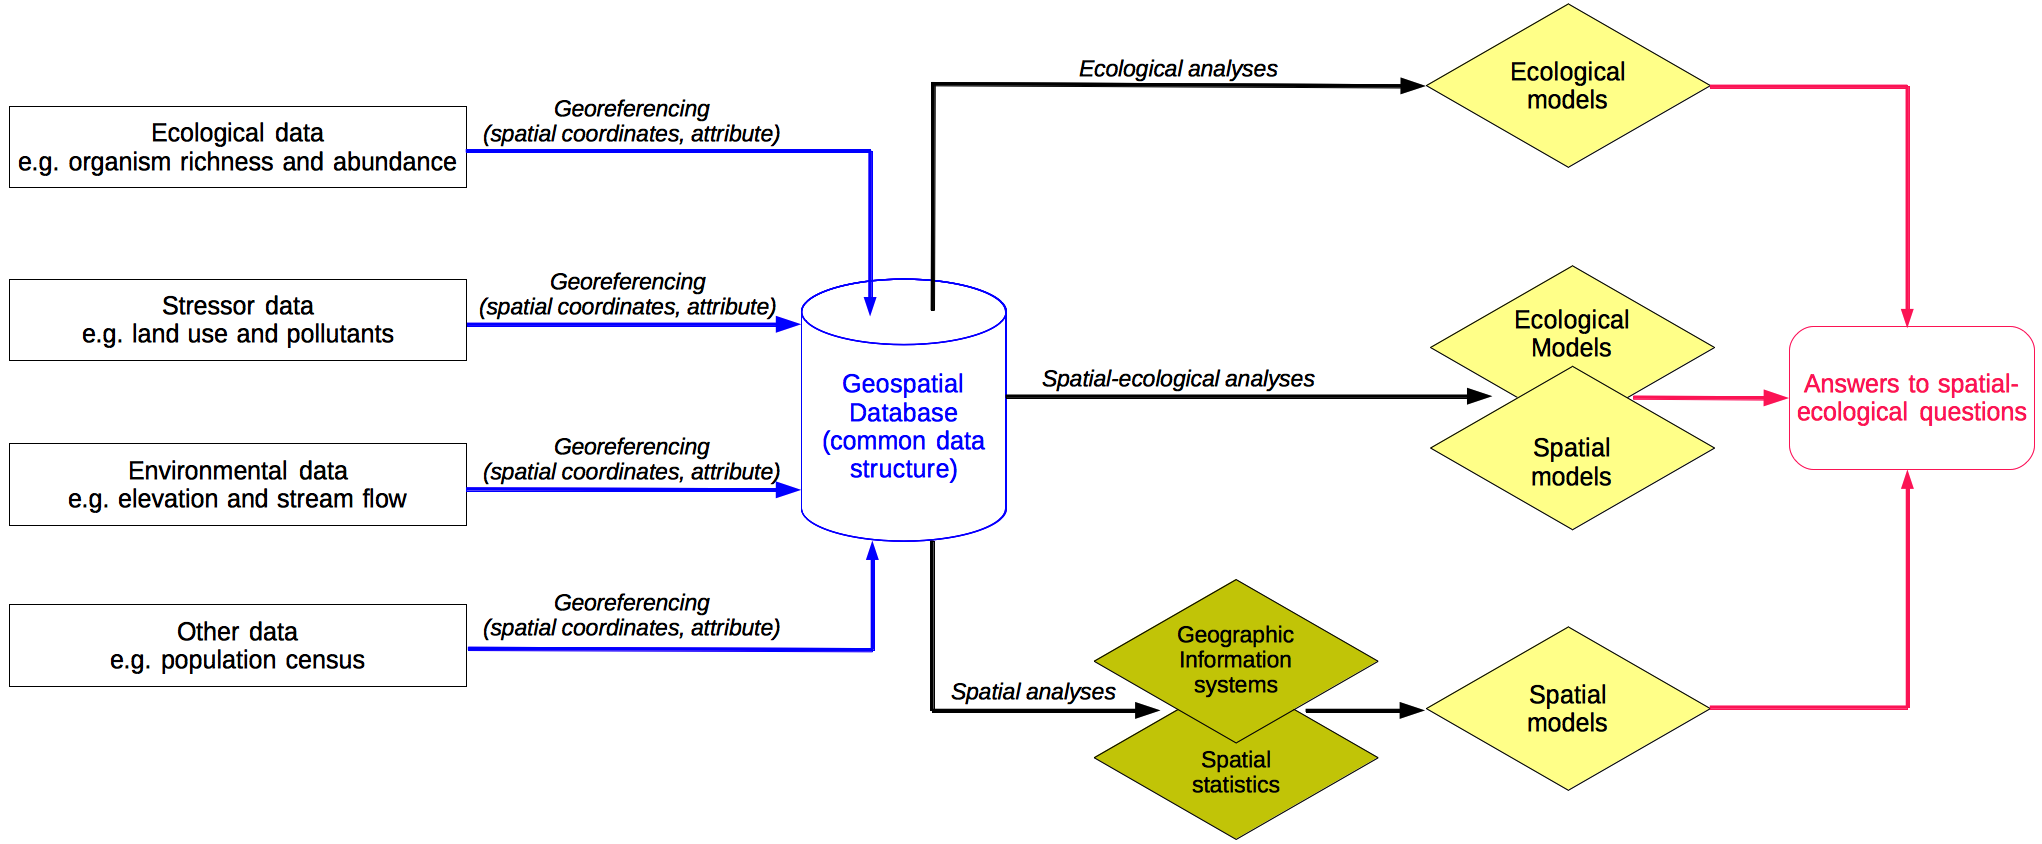
\includegraphics[width=\linewidth]{Figures/Fig_1_1.png}
  \caption{Integration of spatial models with ecological models for spatial-ecological analyses (adopted from the description in Vogiatzakis (2003)).}
  \label{Fig_1_1}
\end{figure}

\noindent not sampled (Webster and Oliver, 2007). Geostatistical interpolation techniques, e.g. kriging\textsuperscript{\textbf{2}}, have been extensively applied for the prediction of variability and magnitude of these indices at non-sampled locations (Hengl, 2009). Spatial variograms\textsuperscript{\textbf{2}}, which model spatial variability of indices, play a central role in geostatistical interpolation, and the number and density of observations in a region are crucial for precise variogram estimation (Webster and Oliver, 2007). In developing countries, observations are often scarce and sparsely distributed because of constrained resources that lead to an unsatisfactory precision of variogram estimation (Goovaerts, 1997; Parajka et al., 2015). Pooled variogram estimation (see chapter 3 for details), which is conducted by comparing spatial variability from multiple time steps, e.g. years, in the presence of time series data, delivers a considerable increase in precision of variogram estimation

\end{landscape}

\noindent\fcolorbox{white}{Gray}{

\begin{minipage}{\textwidth}

\begin{description}

\item[3. Digital elevation model (DEM)] --- A digital elevation model (DEM) is a digital model of the earth surface created from terrain elevation (height from the mean sea level) data (Li et al., 2004). Generally, they are represented as rasters (collection of square grids), where each raster cell represents a location on the earth surface and contains height information of that location. The size of the cell is called resolution and represents the level of details of information in a DEM. However, DEMs can also be represented by a vector-based triangular irregular network (TIN). DEMs are also interchangeably used as digital terrain model (DTM) and digital surface model (DSM) (Hengl, 2009). Nevertheless, DEMs only contain elevation information of the earth, whereas, DTMs, in addition, contain information on the shape of the earth and containing objects, and DSMs contain bare earth shape information. DEMs are generally created using remote sensing techniques, i.e. based on the imageries taken by interferometric synthetic aperture radars boarded on airplanes or earth observation satellites, e.g. ASTER (NASA and METI, 2009; Wise, 2007). They provide important information on earth surface pattern and terrain characteristics that are frequently used in many research fields, e.g. hydrology, cartography and geography (Saunders, 2000).

\end{description}

\end{minipage}}

\bigskip

\noindent under data scarcity (Schuurmans et al., 2007; Wagner et al., 2012). However, the available method for pooled variogram estimation averages variograms estimated for individual time steps that are not suitable for time series with varying spatial locations and number of data points (typical case for developing countries) (Goovaerts, 1997; Gräler et al., 2011). Hence, to increase the precision of pooled variogram estimation, an alternative method is required that account for the variable number and locations of data points in a time series.

\section{Large scale spatial relationship between biological quality elements and drivers}
\label{Large scale spatial relationship between biological quality elements and drivers}

Freshwater organism groups have frequently been used as biological quality elements (BQE) for computation of indices, which are used to indicate the ecological status of freshwater bodies (EC, 2010; Kenney et al., 2009). Especially, traits\textsuperscript{\textbf{4}} of organism groups have shown considerable potential as indicators of multiple stressor effects in freshwater ecosystems (Kenney et al., 2009; Statzner and Bêche, 2010; Van den Brink et al., 2011). They have exhibited substantially less variation than taxonomic groups and hence, demonstrate particularly high suitability for large scale assessment of freshwater degradation and stressor effects (Bonada et al., 2007). Traits have successfully indicated pollution from toxic sediments (Archaimbault et al., 2009), alteration in catchment land use (Larsen and Ormerod, 2010), climate change (Lawrence et al., 2010), salinity and habitat degradation (Díaz et al., 2007), nutrient loads (Dolédec et al., 2006), organic contamination and hydrological disturbances (Feio and Dolédec, 2012) across spatial scales. They also demonstrated high predictive potential for recovery of organisms from degradation (Shipley et al., 2006) and were shown to provide links to important ecosystem functions and services (Mlambo, 2014; Vandewalle et al., 2010).

Many studies have used \textit{a priori} traits of freshwater organisms as biotic indicators of degradation and to disentangle effects of multiple stressors. For example, trait-based approaches have been applied to identify ecological risk from cooccurrences of stressors (Davies and Jackson, 2006), pesticides (Liess et al., 2008), salinity (Kefford et al., 2006) and organic toxicants (Beketov and Liess, 2008; Ohe et al., 2009). Moreover, traits that were hypothesized to be vulnerable to climate change were used to identify organism groups and stream sites that may potentially be at the highest risk of the adverse effects of climate change (Conti et al., 2013; Sandin et al., 2014). However, the spatial relationship between organismal traits and these drivers have rarely been examined on large scales. This limits our macroecological knowledge of the potential spatial responses of organismal traits to large scale drivers, which is important for understanding the change in large scale distribution patterns of freshwater communities under stress (Dray et al., 2012; Heino et al., 2013).

\bigskip

\noindent\fcolorbox{white}{Gray}{

\begin{minipage}{\textwidth}

\begin{description}

\item[4. Traits] --- Traits are biological (phenotypic) and ecological attributes that corresponds to individual and average states of organisms (Van den Brink et al., 2011). These attributes evolve from a number of developmental, morphological, physiological and behavioral adaptations of organisms to their environment (Lancaster and Downes, 2010a, 2010b). Biological traits refer to the life history characteristics, e.g. body size, life cycle, feeding habits and reproduction, whereas ecological traits refer to the ecological preferences of organisms, e.g. habitat, current and temperature preferences (Vandewalle et al., 2010). Traits represent functional characteristics of organisms and thus promote mechanistic understanding of biological communities in a taxon independent manner (Mlambo, 2014; Vandewalle et al., 2010). Hence, trait information can be compared across ecosystems and used to establish links between community and ecosystem ecology (Schmera et al., 2015). A typical trait database contains the affinity (score) of organisms or organism groups to certain traits that are grouped under representative features, e.g. body sizes of $<$ 0.25 cm and 0.25 - 0.50 cm are grouped under the body size featuring group. The largest trait database for European freshwater species is “Freshwater Ecology” (\href{http://www.freshwaterecology.info/}{http://www.freshwaterecology.info/}).

\end{description}

\end{minipage}}

\section{Large scale human and ecological risk assessment}
\label{Large scale human and ecological risk assessment}

Large scale human and ecological risk assessments from stressors, such as contaminants are essential for identification of potential hot spots to develop management strategies and reduce anthropogenic inputs (EEA, 2012). Moreover, the total population at risk from multiple stressors need to be identified for remediation of contaminated areas (Srinivasa and Govil, 2007). However, due to the unavailability of large scale (nationwide, continental and global) contaminant monitoring data, large scale risk assessment are often impeded (Malaj et al., 2014). For example, planetary boundary for global chemical contamination could not be determined although effects on ecosystem health have been evidenced on a global scale (Rockström et al., 2009; Steffen et al., 2015). Especially, in developing countries, resource constraints often limit water quality monitoring activities to a few locations and hence, nationwide risk assessments are often not available and information on the extent of stress and the total population at risk is largely unknown (Azizullah et al., 2011; Törnqvist et al., 2011). Moreover, the monitoring is often biased against rural and remote areas, where people having the least access to water purification measures may be affected by the degradation at upstream urban areas (Khan et al., 2008). Lack of nationwide risk assessments, in turn, impede development of freshwater management frameworks in water-stressed developing countries (MEPA China, 2014; UNEP, 2008). To this end, large scale assessments of human and ecological risks from contaminants are important for the formation of new frameworks in developing countries. While development of large scale contaminant monitoring datasets, e.g. the European Waterbase Dataset (EEA, 2012), are resource and time intensive and in many cases impossible for developing countries, spatial prediction techniques can be employed to fill data gaps for non-sampled locations and enable large scale risk assessments (Javi et al., 2014; Nas and Berktay, 2010).

\section{Aims and objectives}
\label{Aims and objectives}

This Ph.D. thesis aims at: (i) developing novel spatial tools and methods for catchment and regional scale quantification of stressors, (ii) examining large scale relationships between freshwater assemblage traits and drivers by integrating spatial models with ecological models, and (iii) assessing nationwide human health risks from contaminants in data scarce developing countries. Four studies have been conducted using large scale datasets covering three global regions (Figure 1.2), which are presented in chapters 2 – 5 (see Figure 1.3 for the workflow of this thesis).

In chapter 2, an automated and open-source tool is outlined for accumulation threshold (AT) selection that enables objective stream network extraction and upstream riparian corridor (URC) delineation for given stream sampling points from digital elevation models. The objectives of this study were:

\begin{itemize}
\item to develop an algorithm for an automatic and objective selection of ATs by ensuring the highest concordance between DEM extracted and traditionally mapped stream networks
\item to develop an algorithm for automatic and accurate delineation of URCs for given SSPs and sizes, by snapping SSPs to DEM extracted and approximated stream networks
\item to validate and test these algorithms for large scale datasets
\end{itemize}

Chapter 3 outlines an alternative method for pooled within-time series variogram estimation for scarce hydrological data by spatially shifting temporal data points. Specific objectives were:

\begin{itemize}
\item to develop an alternative method for pooled variogram estimation that account for variable numbers and location of data points in a time series
\item to compare the precision of variogram estimation of the developed method with the available method in a data scarce region
\end{itemize}

Large scale relationships between aquatic insect assemblage traits and climate are described in chapter 4, which were established using biomonitoring data from 4,752 German stream sites and 35 global bioclimatic indices (BIs). Spatial variability and autocorrelation in the distribution of aquatic insects were quantified and checked for their association with the BIs. The objectives of this study were:

\begin{itemize}
\item to identify traits and insect groups showing the strongest spatial relationship with the global BIs
\item to identify traits and insect groups showing the highest potential for changing distribution under future climate change
\end{itemize}

\vspace{-0.5cm}\noindent\begin{figure}[h!]
  \centering
  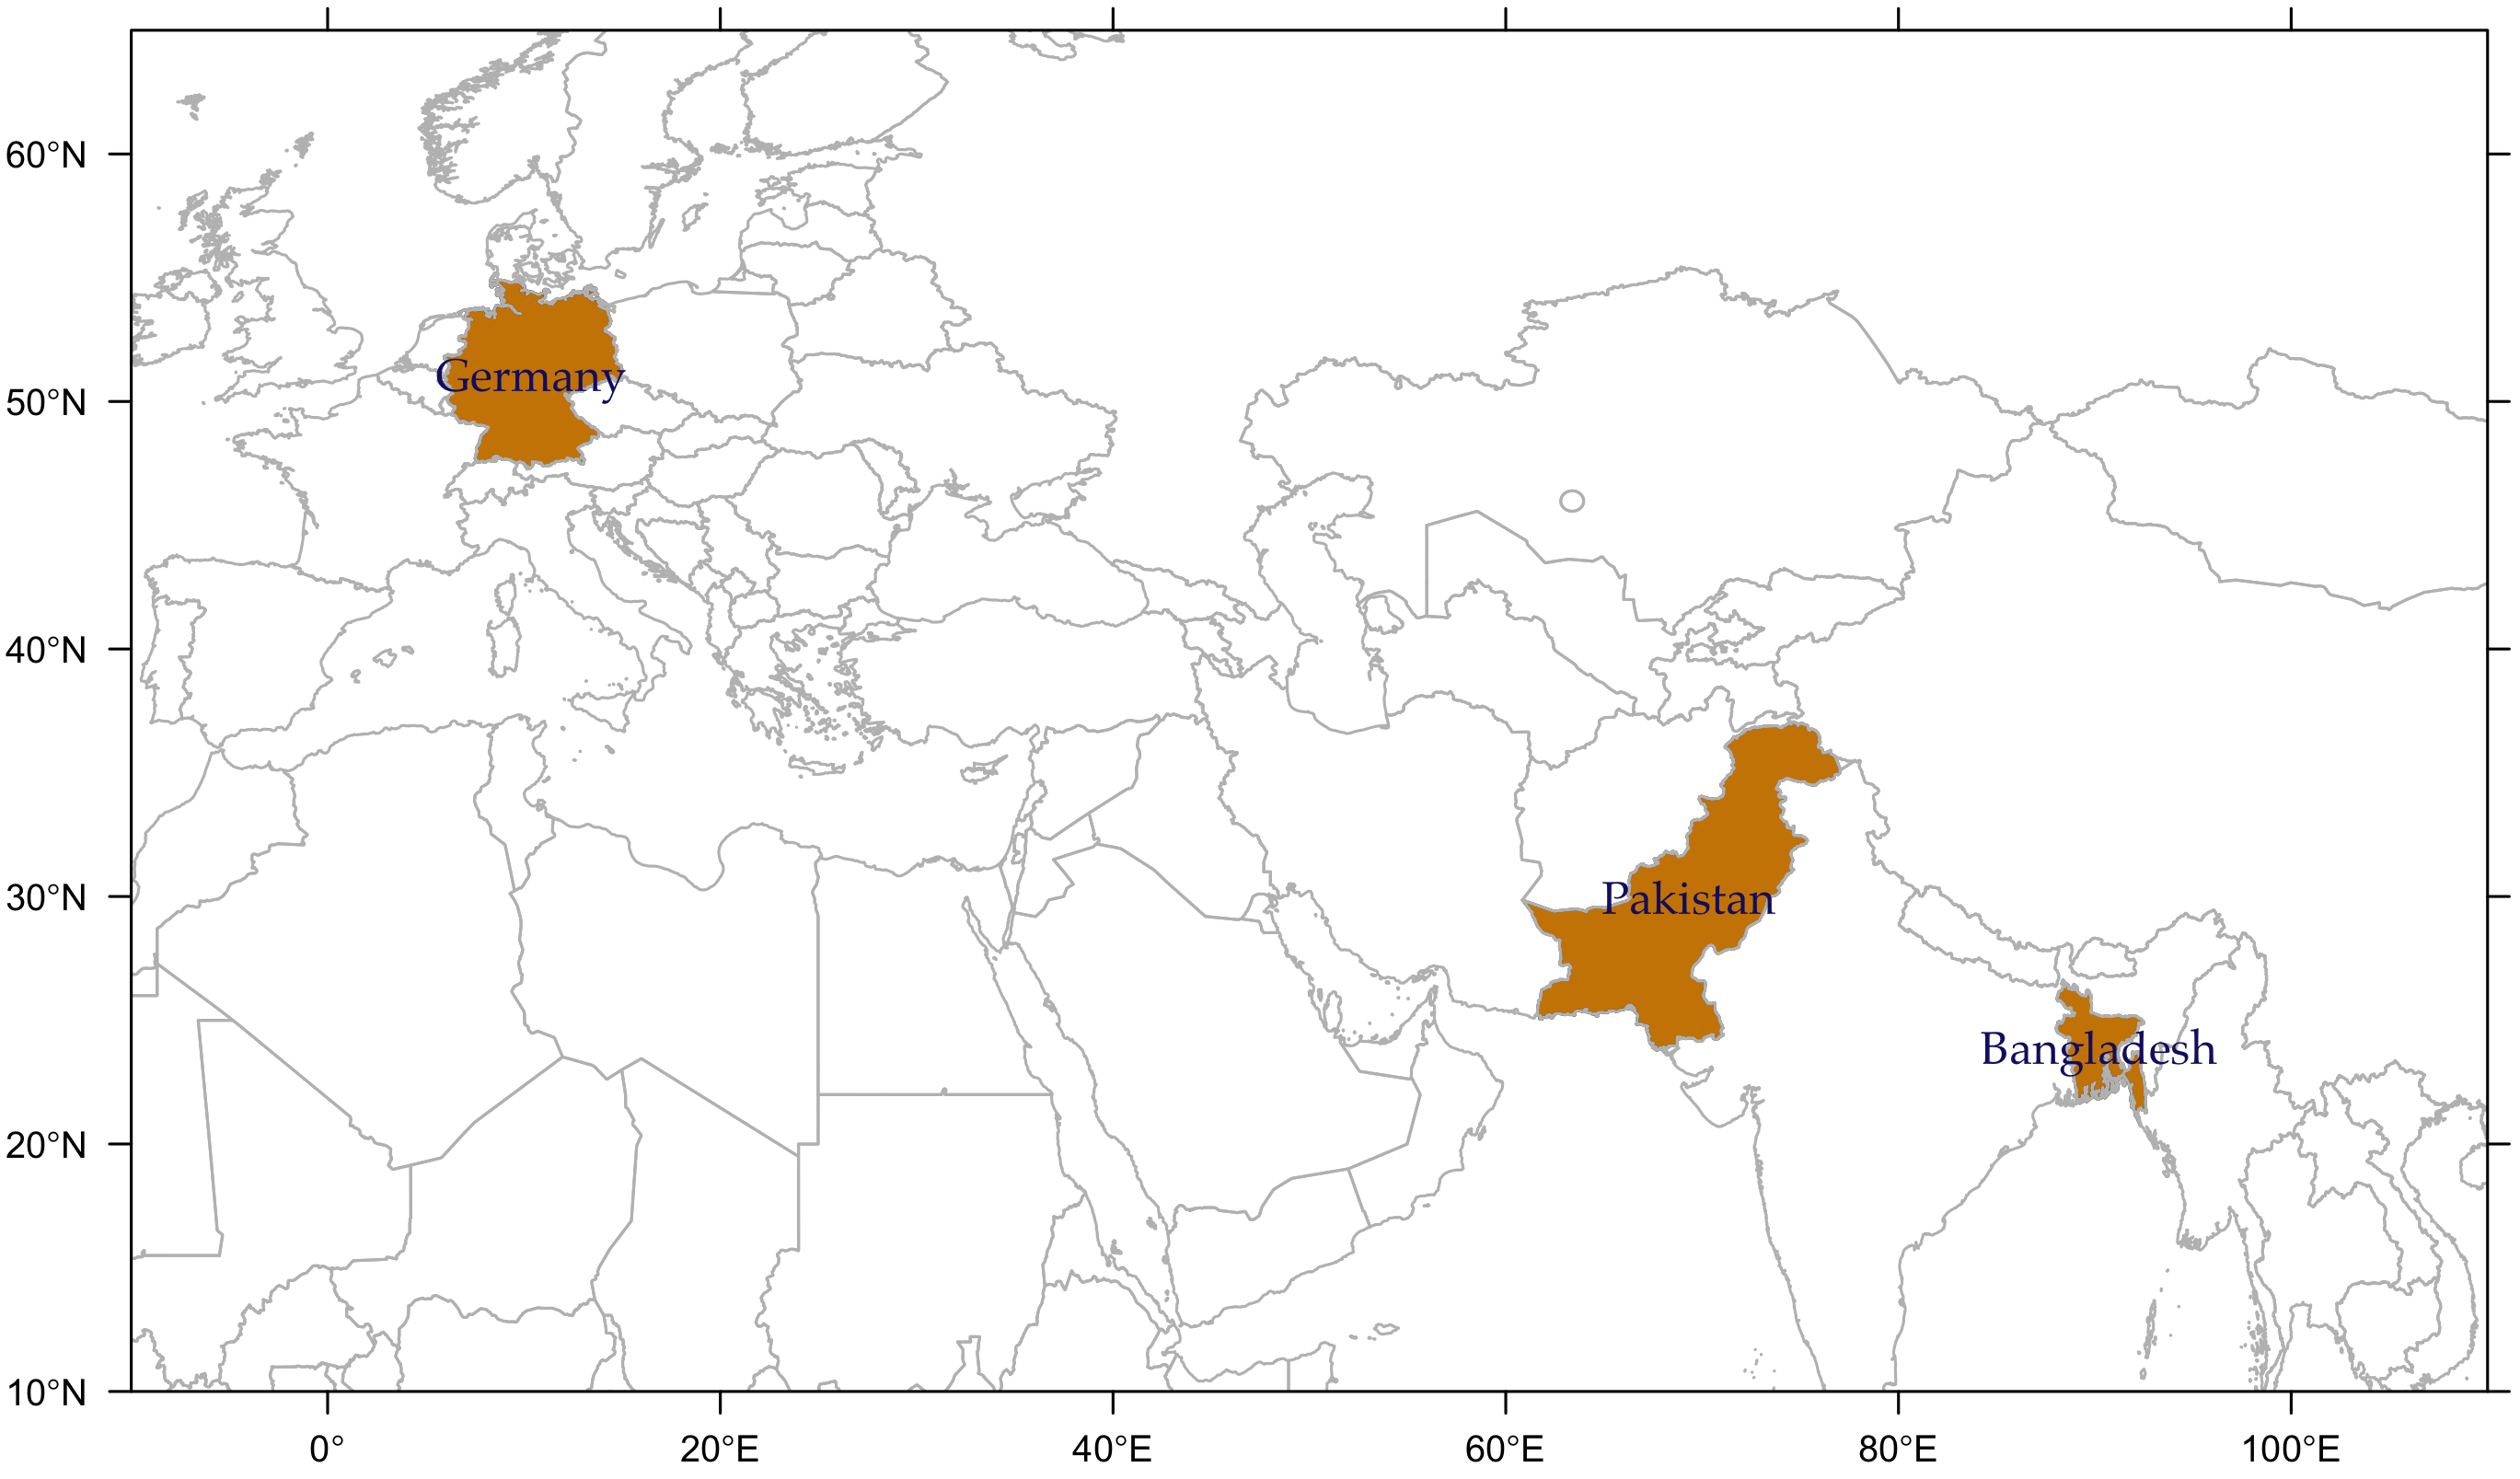
\includegraphics[width=\linewidth]{Figures/Fig_1_2.png}
  \caption{Three global regions (highlighted in orange) covered by the studies in this thesis.}
  \label{Fig_1_2}
\end{figure}

\clearpage

\noindent\begin{figure}[h!]
  \centering
  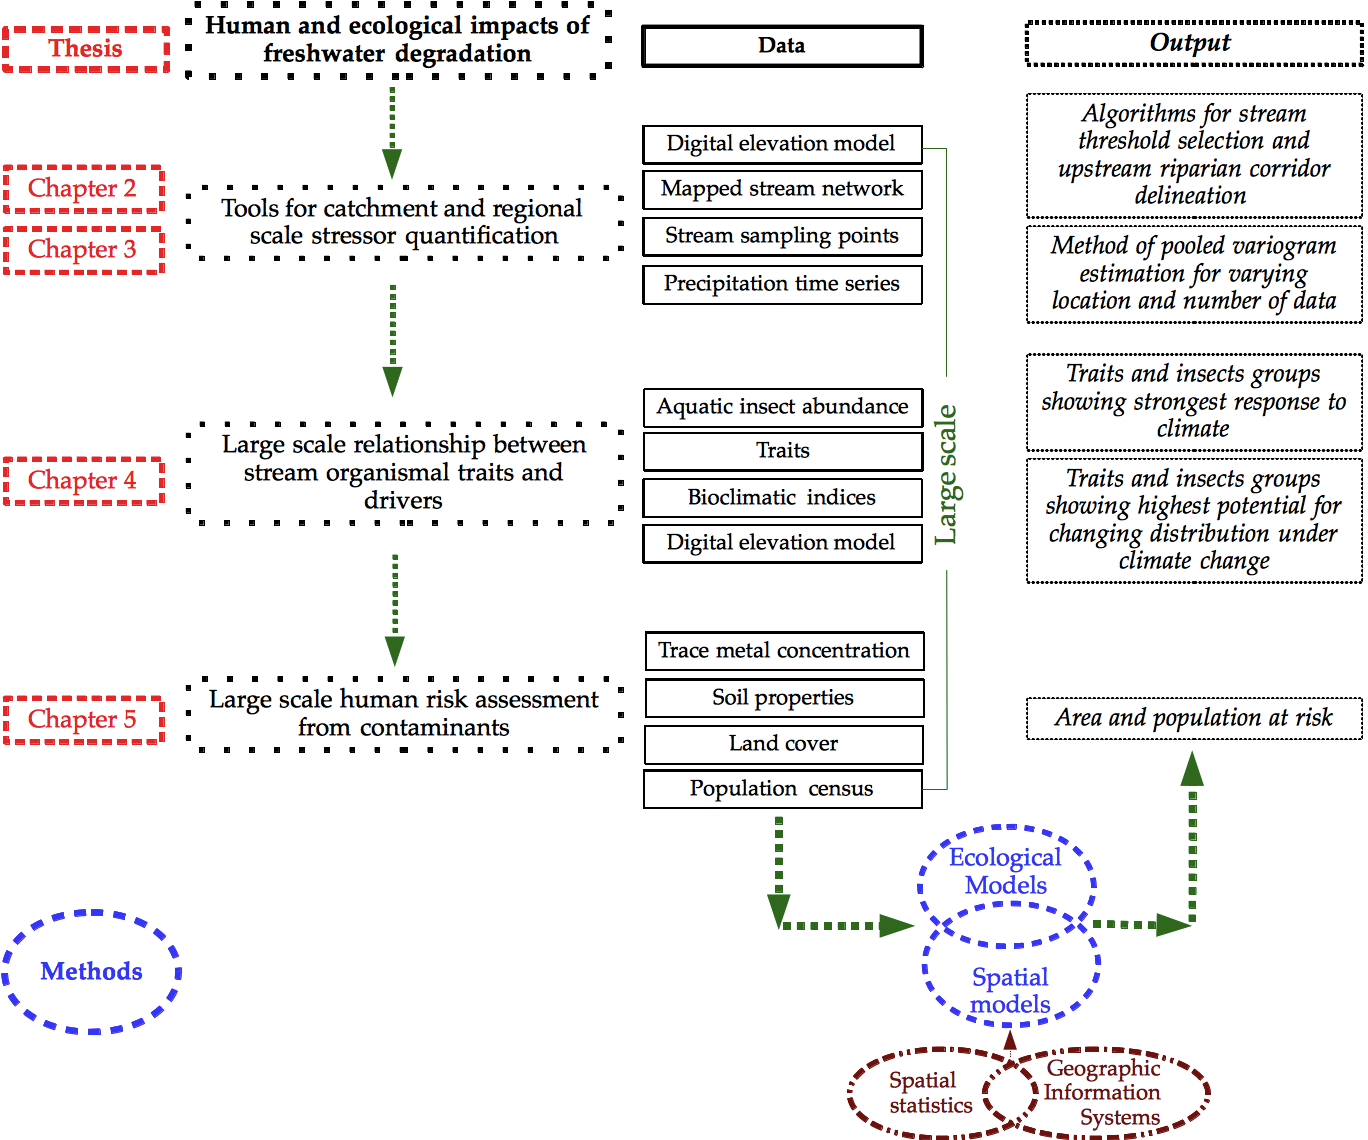
\includegraphics[width=\linewidth]{Figures/Fig_1_3.png}
  \caption{Schematic diagram of the work-flow of this thesis}
  \label{Fig_1_3}
\end{figure}

Finally, a large scale human health risk assessment is described in chapter 5 from trace metal contamination of drinking water sources in Pakistan. A spatial prediction technique that accounts for data scarcity and thus large distances between samples was employed with several spatial predictors for large scale prediction of trace metal concentrations in ground and surface water. The predicted concentrations were compared to the guideline values for drinking water to assess human health risk and quantify total area and population at risk. The objectives were:

\begin{itemize}
\item to predict the concentrations of 10 trace metal in ground and surface water by employing an appropriate spatial prediction technique on previously published data for a few administrative area and using relevant spatial predictors
\item to use predicted trace metal concentrations for nationwide human health risk assessment by comparing with guideline values and quantify total area and population at risk.
\end{itemize}

\begingroup

\renewcommand{\addcontentsline}[3]{}

\begin{thebibliography}

\bibitem{} \hangindent=1cm Abood, S.A., Maclean, A.L., Mason, L.A., 2012. Modeling Riparian Zones Utilizing DEMS and Flood Height Data. Photogrammetric engineering and remote sensing 78, 259–269.

\bibitem{} \hangindent=1cm Anselin, L., 1989. What is special about spatial data?: alternative perspectives on spatial data analysis. Presented at the Spatial Statistics, Past, Present and Future, Syracuse.

\bibitem{} \hangindent=1cm Archaimbault, V., Usseglio-Polatera, P., Garric, J., Wasson, J.-G., Babut, M., 2009. Assessing pollution of toxic sediment in streams using bio-ecological traits of benthic macroinvertebrates: Toxic pollution index and macroinvertebrates. Freshwater Biology 55, 1430–1446. doi:10.1111/j.1365-2427.2009.02281.x

\bibitem{} \hangindent=1cm Azizullah, A., Khattak, M.N.K., Richter, P., Häder, D.-P., 2011. Water pollution in Pakistan and its impact on public health — A review. Environment International 37, 479–497. doi:10.1016/j.envint.2010.10.007

\bibitem{} \hangindent=1cm Beketov, M.A., Liess, M., 2008. An indicator for effects of organic toxicants on lotic invertebrate communities: Independence of confounding environmental factors over an extensive river continuum. Environmental Pollution 156, 980–987. doi:10.1016/j.envpol.2008.05.005

\bibitem{} \hangindent=1cm Biss, R., Kübler, P., Pinter, I., Braukmann, U., 2006. Leitbildbezogenes biozönotisches Bewertungsverfahren für Fließgewässer in der Bundesrepublik Deutschland -Ein erster Beitrag zur integrierten ökologischen Fließgewässerbewertung (Project report No. 298 24 777), UBA-FB 000348. Umweltforschungsplan des Bundesministeriums für Umwelt, Naturschutz und Reaktorsicherheit, Berlin.

\bibitem{} \hangindent=1cm Bonada, N., DoléDec, S., Statzner, B., 2007. Taxonomic and biological trait differences of stream macroinvertebrate communities between mediterranean and temperate regions: implications for future climatic scenarios. Global Change Biology 13, 1658–1671. doi:10.1111/j.1365-2486.2007.01375.x

\bibitem{} \hangindent=1cm Borcard, D., Legendre, P., Avois-Jacquet, C., Tuomisto, H., 2004. Dissecting the spatial structure of ecological data at multiple scales. Ecology 85, 1826–1832.

\bibitem{} \hangindent=1cm Burrough, P.A., Frank, A.U., 1995. Concepts and paradigms in spatial information: are current geographical information systems truly generic? International journal of geographical information systems 9, 101–116. doi:10.1080/02693799508902028

\bibitem{} \hangindent=1cm Canadian Cartographic Association (CCA), 2015. Canadian Cartographic Association [WWW Document]. URL http://cca-acc.org/about-us/ (accessed 8.14.15).

\bibitem{} \hangindent=1cm Carpenter, S.R., Stanley, E.H., Vander Zanden, M.J., 2011. State of the World’s Freshwater Ecosystems: Physical, Chemical, and Biological Changes. Annual Review of Environment and Resources 36, 75–99. doi:10.1146/annurev-environ-021810-094524

\bibitem{} \hangindent=1cm Chiles, J.-P., Delfiner, P., 2012. Geostatistics modeling spatial uncertainty, second edition. John Wiley & Sons, Hoboken, N.J.
Chrisman, N., 2001. Exploring geographical information systems. Wiley.

\bibitem{} \hangindent=1cm Christakos, G., 2000. Modern spatiotemporal geostatistics. Courier Corporation.

\bibitem{} \hangindent=1cm Colson, T., Gregory, J., Dorney, J., Russell, P., 2008. Topographic and soil maps do not accurately depict headwater stream networks. National Wetlands Newsletter 30, 25–28.

\bibitem{} \hangindent=1cm Conti, L., Schmidt-Kloiber, A., Grenouillet, G., Graf, W., 2013. A trait-based approach to assess the vulnerability of European aquatic insects to climate change. Hydrobiologia 721, 297–315. doi:10.1007/s10750-013-1690-7

\bibitem{} \hangindent=1cm Cressie, N., 1993. Statistics for spatial data, Revised edition. ed. John Wiley & Sons, New York, Chichester, Toronto, Brisbane, Singapore.

\bibitem{} \hangindent=1cm Crutzen, P., 2006. The “Anthropocene,” in: Ehlers, E., Krafft, T. (Eds.), Earth System Science in the Anthropocene. Springer Berlin Heidelberg, pp. 13–18.

\bibitem{} \hangindent=1cm Dahm, V., Hering, D., Nemitz, D., Graf, W., Schmidt-Kloiber, A., Leitner, P., Melcher, A., Feld, C.K., 2013. Effects of physico-chemistry, land use and hydromorphology on three riverine organism groups: a comparative analysis with monitoring data from Germany and Austria. Hydrobiologia 704, 389–415. doi:10.1007/s10750-012-1431-3

\bibitem{} \hangindent=1cm Dai, A., Qian, T., Trenberth, K.E., Milliman, J.D., 2009. Changes in continental freshwater discharge from 1948 to 2004. Journal of Climate 22, 2773–2792.

\bibitem{} \hangindent=1cm Davies, S.P., Jackson, S.K., 2006. The biological condition gradient: a descriptive model for interpreting change in aquatic ecosystems. Ecological Applications 16, 1251–1266.

\bibitem{} \hangindent=1cm DíAz, A.M., Alonso, M.L.S., GutiéRrez, M.R.V.-A., 2007. Biological traits of stream macroinvertebrates from a semi-arid catchment: patterns along complex environmental gradients. Freshwater Biology 0, 071204011451001–??? doi:10.1111/j.1365-2427.2007.01854.x

\bibitem{} \hangindent=1cm Dolédec, S., Phillips, N., Scarsbrook, M., Riley, R.H., Townsend, C.R., 2006. Comparison of structural and functional approaches to determining landuse effects on grassland stream invertebrate communities. Journal of the North American Benthological Society 25, 44–60. doi:10.1899/0887-3593(2006)25[44:COSAFA]2.0.CO;2

\bibitem{} \hangindent=1cm Dray, S., Pélissier, R., Couteron, P., Fortin, M.-J., Legendre, P., Peres-Neto, P.R., Bellier, E., Bivand, R., Blanchet, F.G., De Cáceres, M., 2012. Community ecology in the age of multivariate multiscale spatial analysis. Ecological Monographs 82, 257–275. doi:10.1890/11-1183.1

\bibitem{} \hangindent=1cm Dudgeon, D., Arthington, A.H., Gessner, M.O., Kawabata, Z.-I., Knowler, D.J., Lévêque, C., Naiman, R.J., Prieur-Richard, A.-H., Soto, D., Stiassny, M.L.J., Sullivan, C.A., 2005. Freshwater biodiversity: importance, threats, status and conservation challenges. Biological Reviews 81, 163–182. doi:10.1017/S1464793105006950

\bibitem{} \hangindent=1cm Environmental Systems Research Institute (ESRI), Redlands, 2001. What is ArcGIS?: GIS by ESRI. ESRI.

\bibitem{} \hangindent=1cm European Commission (EC), 2013. A blueprint to safeguard Europe’s water resources, NAT.

\bibitem{} \hangindent=1cm European Commission (EC), 2010. Water Framework Directive.

\bibitem{} \hangindent=1cm European Environment Agency (EEA), 2012. European waters - assessment of status and pressures (No. 8/2012). European Environment Agency, Copenhagen.

\bibitem{} \hangindent=1cm Feio, M.J., Dolédec, S., 2012. Integration of invertebrate traits into predictive models for indirect assessment of stream functional integrity: a case study in Portugal. Ecological Indicators 15, 236–247.

\bibitem{} \hangindent=1cm Fernández, D., Barquín, J., Álvarez-Cabria, M., Peñas, F.J., 2012. Quantifying the performance of automated GIS-based geomorphological approaches for riparian zone delineation using digital elevation models. Hydrology and Earth System Sciences 16, 3851–3862. doi:10.5194/hess-16-3851-2012

\bibitem{} \hangindent=1cm Fortin, M.-J., Dale, M.R.T., 2005. Spatial analysis: a guide for ecologists. Cambridge University Press, Cambridge.

\bibitem{} \hangindent=1cm Fortin, M.-J., James, P.M.A., MacKenzie, A., Melles, S.J., Rayfield, B., 2012. Spatial statistics, spatial regression, and graph theory in ecology. Spatial Statistics 1, 100–109. doi:10.1016/j.spasta.2012.02.004

\bibitem{} \hangindent=1cm Gaetan, C., Guyon, X., Bleakley, K., 2010. Spatial statistics and modeling. Springer.

\bibitem{} \hangindent=1cm Goodchild, M.F., 1992. Geographical information science. International journal of geographical information systems 6, 31–45.

\bibitem{} \hangindent=1cm Goovaerts, P., 1997. Geostatistics for natural resources evaluation. Oxford university press.

\bibitem{} \hangindent=1cm Gräler, B., Gerharz, L.E., Pebesma, E., 2011. Spatio-temporal analysis and interpolation of PM10 measurements in Europe (Technical paper No. 2011/10). European Topic Center on Air Pollution and Climate Change Mitigation, Bilthoven.

\bibitem{} \hangindent=1cm GRASS Development Team, 2015. Geographic Resources Analysis Support System (GRASS). Open Source Geospatial Foundation Project.

\bibitem{} \hangindent=1cm Harris, P., Fotheringham, A.S., Crespo, R., Charlton, M., 2010. The Use of Geographically Weighted Regression for Spatial Prediction: An Evaluation of Models Using Simulated Data Sets. Mathematical Geosciences 42, 657–680. doi:10.1007/s11004-010-9284-7

\bibitem{} \hangindent=1cm Heine, R.A., Lant, C.L., Sengupta, R.R., 2004. Development and Comparison of Approaches for Automated Mapping of Stream Channel Networks. Annals of the Association of American Geographers 94, 477–490. doi:10.1111/j.1467-8306.2004.00409.x

\bibitem{} \hangindent=1cm Heino, J., Schmera, D., Erős, T., 2013. A macroecological perspective of trait patterns in stream communities. Freshwater Biology 58, 1539–1555. doi:10.1111/fwb.12164

\bibitem{} \hangindent=1cm Hengl, T., 2009. A Practical Guide to Geostatistical Mapping. University of Amsterdam, Amsterdam.

\bibitem{} \hangindent=1cm Holmes, K.L., Goebel, P.C., 2011. A functional approach to riparian area delineation using geospatial methods. Journal of Forestry 109, 233–241.

\bibitem{} \hangindent=1cm Huang, J., Huang, Y., Pontius, R.G., Zhang, Z., 2015. Geographically weighted regression to measure spatial variations in correlations between water pollution versus land use in a coastal watershed. Ocean & Coastal Management 103, 14–24. doi:10.1016/j.ocecoaman.2014.10.007

\bibitem{} \hangindent=1cm Hugueny, B., Oberdorff, T., Tedesco, P.A., 2010. Community ecology of river fishes: a large-scale perspective, in: American Fisheries Society Symposium. pp. 29–62.

\bibitem{} \hangindent=1cm International Union for Conservation of Nature (IUCN), 2015. International Union for Conservation of Nature [WWW Document]. URL http://www.iucn.org/ (accessed 8.13.15).

\bibitem{} \hangindent=1cm Javi, S.T., Malekmohammadi, B., Mokhtari, H., 2014. Application of geographically weighted regression model to analysis of spatiotemporal varying relationships between groundwater quantity and land use changes (case study: Khanmirza Plain, Iran). Environmental Monitoring and Assessment 186, 3123–3138. doi:10.1007/s10661-013-3605-5

\bibitem{} \hangindent=1cm Kefford, B.J., Nugegoda, D., Metzeling, L., Fields, E.J., 2006. Validating species sensitivity distributions using salinity tolerance of riverine macroinvertebrates in the southern Murray-Darling Basin (Victoria, Australia). Canadian Journal of Fisheries and Aquatic Sciences 63, 1865–1877.

\bibitem{} \hangindent=1cm Kenney, M.A., Sutton-Grier, A.E., Smith, R.F., Gresens, S.E., 2009. Benthic macroinvertebrates as indicators of water quality: The intersection of science and policy. Terrestrial Arthropod Reviews 2, 99–128. doi:10.1163/187498209X12525675906077

\bibitem{} \hangindent=1cm Khan, S., Cao, Q., Zheng, Y.M., Huang, Y.Z., Zhu, Y.G., 2008. Health risks of heavy metals in contaminated soils and food crops irrigated with wastewater in Beijing, China. Environmental Pollution 152, 686–692. doi:10.1016/j.envpol.2007.06.056

\bibitem{} \hangindent=1cm Lagacherie, P., Rabotin, M., Colin, F., Moussa, R., Voltz, M., 2010. Geo-MHYDAS: A landscape discretization tool for distributed hydrological modeling of cultivated areas. Computers & Geosciences 36, 1021–1032. doi:10.1016/j.cageo.2009.12.005

\bibitem{} \hangindent=1cm Lancaster, J., Downes, B.J., 2010a. Linking the hydraulic world of individual organisms to ecological processes: Putting ecology into ecohydraulics. River Research and Applications 26, 385–403. doi:10.1002/rra.1274

\bibitem{} \hangindent=1cm Lancaster, J., Downes, B.J., 2010b. Ecohydraulics needs to embrace ecology and sound science, and to avoid mathematical artefacts. River Research and Applications 26, 921–929. doi:10.1002/rra.1425

\bibitem{} \hangindent=1cm Larsen, S., Ormerod, S.J., 2010. Combined effects of habitat modification on trait composition and species nestedness in river invertebrates. Biological Conservation 143, 2638–2646. doi:10.1016/j.biocon.2010.07.006

\bibitem{} \hangindent=1cm Lawrence, J.E., Lunde, K.B., Mazor, R.D., Bêche, L.A., McElravy, E.P., Resh, V.H., 2010. Long-term macroinvertebrate responses to climate change: implications for biological assessment in mediterranean-climate streams. Journal of the North American Benthological Society 29, 1424–1440. doi:10.1899/09-178.1

\bibitem{} \hangindent=1cm Legendre, P., 1993. Spatial Autocorrelation: Trouble or New Paradigm? Ecology 74, 1659. doi:10.2307/1939924

\bibitem{} \hangindent=1cm Legendre, P., Fortin, M.J., 1989. Spatial pattern and ecological analysis. Vegetatio 80, 107–138.

\bibitem{} \hangindent=1cm Legendre, P., Legendre, L.F., 1998. Numerical ecology. Elsevier.

\bibitem{} \hangindent=1cm Liess, M., Schäfer, R.B., Schriever, C.A., 2008. The footprint of pesticide stress in communities—Species traits reveal community effects of toxicants. Science of The Total Environment 406, 484–490. doi:10.1016/j.scitotenv.2008.05.054

\bibitem{} \hangindent=1cm Lin, W.T., Chou, W.C., Lin, C.Y., Huang, P.H., Tsai, J.S., 2006. Automated suitable drainage network extraction from digital elevation models in Taiwan’s upstream watersheds. Hydrological Processes 20, 289–306. doi:10.1002/hyp.5911

\bibitem{} \hangindent=1cm Li, Z., Zhu, C., Gold, C., 2004. Digital terrain modeling: principles and methodology. CRC press.

\bibitem{} \hangindent=1cm Lorenz, A.W., Feld, C.K., 2013. Upstream river morphology and riparian land use overrule local restoration effects on ecological status assessment. Hydrobiologia 704, 489–501. doi:10.1007/s10750-012-1326-3

\bibitem{} \hangindent=1cm Lovett, S., Price, P., Edgar, B., 2007. Salt, nutrient, sediment and interactions: findings from the National River contaminants program. Land and Water Australia, Canberra, A.C.T.

\bibitem{} \hangindent=1cm Malaj, E., Peter, C., Grote, M., Kühne, R., Mondy, C.P., Usseglio-Polatera, P., Brack, W., Schäfer, R.B., 2014. Organic chemicals jeopardize the health of freshwater ecosystems on the continental scale. Proceedings of the National Academy of Sciences 201321082.

\bibitem{} \hangindent=1cm Marzin, A., Verdonschot, P.F.M., Pont, D., 2013. The relative influence of catchment, riparian corridor, and reach-scale anthropogenic pressures on fish and macroinvertebrate assemblages in French rivers. Hydrobiologia 704, 375–388. doi:10.1007/s10750-012-1254-2

\bibitem{} \hangindent=1cm McLeman, R., Smit, B., 2006. Migration as an Adaptation to Climate Change. Climatic Change 76, 31–53. doi:10.1007/s10584-005-9000-7

\bibitem{} \hangindent=1cm Millennium Ecosystem Assessment (MEA), 2005. Ecosystems and human well-being: wetlands and water (Synthesis). World Resources Institute, Washington, D.C.

\bibitem{} \hangindent=1cm Ministry of Environmental Protection, the People’s Republic of China (MEPA China), 2014. The State of the Environment of China in 2013 [WWW Document]. URL http://english.mep.gov.cn/ (accessed 8.13.15).

\bibitem{} \hangindent=1cm Mlambo, M.C., 2014. Not all traits are “functional”: insights from taxonomy and biodiversity-ecosystem functioning research. Biodiversity and Conservation 23, 781–790. doi:10.1007/s10531-014-0618-5

\bibitem{} \hangindent=1cm Nas, B., Berktay, A., 2010. Groundwater quality mapping in urban groundwater using GIS. Environmental Monitoring and Assessment 160, 215–227. doi:10.1007/s10661-008-0689-4

\bibitem{} \hangindent=1cm National Aeronautics and Space Administration (NASA), Japan’s Ministry of Economy, Trade and Industry (METI), 2009. ASTER Global Digital Elevation Map [WWW Document]. URL http://asterweb.jpl.nasa.gov/gdem.asp (accessed 12.18.13).

\bibitem{} \hangindent=1cm National Land & Water Resources Audit, Australia (NLWRA), 2002. Australian catchment, river, and estuary assessment 2002: assessing the aggregate impact of resource use on key natural ecosystems. (No. ISBN: 0 642 37125 3). National Land & Water Resources Audit, Canberra ACT.

\bibitem{} \hangindent=1cm Ohe, P.C. von der, De Deckere, E., Prü\s s, A., Muñoz, I., Wolfram, G., Villagrasa, M., Ginebreda, A., Hein, M., Brack, W., 2009. Toward an integrated assessment of the ecological and chemical status of European river basins. Integrated environmental assessment and management 5, 50–61.

\bibitem{} \hangindent=1cm Parajka, J., Merz, R., Skøien, J.O., Viglione, A., 2015. The role of station density for predicting daily runoff by top-kriging interpolation in Austria 63. doi:10.1515/johh-2015-0024

\bibitem{} \hangindent=1cm Parent, P., Church, R., 1987. Evolution of Geographic Information Systems as Decision Making Tools, in: Proceedings of the 2nd Annual Conference on Geographic Information Systems. Presented at the 2nd Annual Conference on Geographic Information Systems, San Francisco, pp. 63–71.

\bibitem{} \hangindent=1cm Pereira, H.M., Leadley, P.W., Proenca, V., Alkemade, R., Scharlemann, J.P.W., Fernandez-Manjarres, J.F., Araujo, M.B., Balvanera, P., Biggs, R., Cheung, W.W.L., Chini, L., Cooper, H.D., Gilman, E.L., Guenette, S., Hurtt, G.C., Huntington, H.P., Mace, G.M., Oberdorff, T., Revenga, C., Rodrigues, P., Scholes, R.J., Sumaila, U.R., Walpole, M., 2010. Scenarios for Global Biodiversity in the 21st Century. Science 330, 1496–1501. doi:10.1126/science.1196624

\bibitem{} \hangindent=1cm Pollard, A.I., Yuan, L., 2006. Community response patterns: evaluating benthic invertebrate composition in metal-polluted streams. Ecological Applications 16, 645–655.

\bibitem{} \hangindent=1cm R Development Core Team, 2015. R: A language and environment for statistical computing. R Foundation for Statistical Computing. Vienna, Austria.

\bibitem{} \hangindent=1cm Reuveny, R., 2007. Climate change-induced migration and violent conflict. Political Geography 26, 656–673. doi:10.1016/j.polgeo.2007.05.001

\bibitem{} \hangindent=1cm Rockström, J., Steffen, W.L., Noone, K., Persson, \AAsa, Chapin III, F.S., Lambin, E., Lenton, T.M., Scheffer, M., Folke, C., Schellnhuber, H.J., others, 2009. Planetary boundaries: exploring the safe operating space for humanity.

\bibitem{} \hangindent=1cm Sandin, L., Schmidt-Kloiber, A., Svenning, J.-C., Jeppesen, E., Friberg, N., 2014. A trait-based approach to assess climate change sensitivity of freshwater invertebrates across Swedish ecoregions. Current Zoology 60.

\bibitem{} \hangindent=1cm Saunders, W., 2000. Preparation of DEMs for use in environmental modeling analysis. Hydrologic and hydraulic modeling support with geographic information systems. ESRI Press, New York 29–52.

\bibitem{} \hangindent=1cm Schmera, D., Podani, J., Heino, J., Erős, T., Poff, N.L., 2015. A proposed unified terminology of species traits in stream ecology. Freshwater Science 000–000. doi:10.1086/681623

\bibitem{} \hangindent=1cm Schuurmans, J.M., Bierkens, M.F.P., Pebesma, E.J., Uijlenhoet, R., 2007. Automatic Prediction of High-Resolution Daily Rainfall Fields for Multiple Extents: The Potential of Operational Radar. Journal of Hydrometeorology 8, 1204–1224. doi:10.1175/2007JHM792.1

\bibitem{} \hangindent=1cm Shipley, B., Vile, D., Garnier, E., 2006. From Plant Traits to Plant Communities: A Statistical Mechanistic Approach to Biodiversity. Science 314, 812–814. doi:10.1126/science.1131344

\bibitem{} \hangindent=1cm Skøien, J.O., Blöschl, G., Laaha, G., Pebesma, E., Parajka, J., Viglione, A., 2014. rtop: an R package for interpolation of data with a variable spatial support, with an example from river networks. Computers & Geosciences. doi:10.1016/j.cageo.2014.02.009

\bibitem{} \hangindent=1cm Srinivasa, S.G., Govil, P.K., 2007. Distribution of heavy metals in surface water of Ranipet industrial area in Tamil Nadu, India. Environmental Monitoring and Assessment 136, 197–207. doi:10.1007/s10661-007-9675-5

\bibitem{} \hangindent=1cm Statzner, B., Bêche, L.A., 2010. Can biological invertebrate traits resolve effects of multiple stressors on running water ecosystems? Freshwater Biology 55, 80–119. doi:10.1111/j.1365-2427.2009.02369.x

\bibitem{} \hangindent=1cm Steffen, W., Richardson, K., Rockstrom, J., Cornell, S.E., Fetzer, I., Bennett, E.M., Biggs, R., Carpenter, S.R., de Vries, W., de Wit, C.A., Folke, C., Gerten, D., Heinke, J., Mace, G.M., Persson, L.M., Ramanathan, V., Reyers, B., Sorlin, S., 2015. Planetary boundaries: Guiding human development on a changing planet. Science 347, 1259855–1259855. doi:10.1126/science.1259855

\bibitem{} \hangindent=1cm Stehle, S., Schulz, R., 2015. Agricultural insecticides threaten surface waters at the global scale. Proceedings of the National Academy of Sciences 112, 5750–5755. doi:10.1073/pnas.1500232112

\bibitem{} \hangindent=1cm Stevens Jr, D.L., Olsen, A.R., 2004. Spatially balanced sampling of natural resources. Journal of the American Statistical Association 99, 262–278.

\bibitem{} \hangindent=1cm Stocker, T.F., Dahe, Q., Plattner, G.-K., 2013. Climate Change 2013: The Physical Science Basis, Working Group I Contribution to the Fifth Assessment Report of the Intergovernmental Panel on Climate Change. Summary for Policymakers. Intergovernmental Panel on Climate Change (IPCC).

\bibitem{} \hangindent=1cm Tarboton, D.G., Bras, R.L., Rodriguez-Iturbe, I., 1991. On the extraction of channel networks from digital elevation data. Hydrological processes 5, 81–100.

\bibitem{} \hangindent=1cm Tobler, W.R., 1970. A Computer Movie Simulating Urban Growth in the Detroit Region. Economic Geography 46, 234. doi:10.2307/143141

\bibitem{} \hangindent=1cm Törnqvist, R., Jarsjö, J., Karimov, B., 2011. Health risks from large-scale water pollution: trends in Central Asia. Environment International 37, 435–442.

\bibitem{} \hangindent=1cm United Nations Environment Programme (UNEP), 2015. United Nations Environment Programme [WWW Document]. URL http://www.unep.org/ (accessed 5.1.15).

\bibitem{} \hangindent=1cm United Nations Environment Programme (UNEP), 2008. Freshwater Under Threat. South Asia. Vulnerability Assessment of Freshwater Resources to Envrionmental Change. Kenya.

\bibitem{} \hangindent=1cm United States Environmental Protection Agency (USEPA), 2015. Watershed Assessment, Tracking & Environmental Results [WWW Document]. National Summary of State Information. URL http://ofmpub.epa.gov/waters10/attains_nation_cy.control (accessed 1.28.15).

\bibitem{} \hangindent=1cm Utz, R.M., Hilderbrand, R.H., Boward, D.M., 2009. Identifying regional differences in threshold responses of aquatic invertebrates to land cover gradients. Ecological Indicators 9, 556–567. doi:10.1016/j.ecolind.2008.08.008

\bibitem{} \hangindent=1cm Van den Brink, P.J., Alexander, A.C., Desrosiers, M., Goedkoop, W., Goethals, P.L., Liess, M., Dyer, S.D., 2011. Traits-based approaches in bioassessment and ecological risk assessment: Strengths, weaknesses, opportunities and threats. Integrated Environmental Assessment and Management 7, 198–208. doi:10.1002/ieam.109

\bibitem{} \hangindent=1cm Vandewalle, M., Bello, F., Berg, M.P., Bolger, T., Dolédec, S., Dubs, F., Feld, C.K., Harrington, R., Harrison, P.A., Lavorel, S., Silva, P.M., Moretti, M., Niemelä, J., Santos, P., Sattler, T., Sousa, J.P., Sykes, M.T., Vanbergen, A.J., Woodcock, B.A., 2010. Functional traits as indicators of biodiversity response to land use changes across ecosystems and organisms. Biodiversity and Conservation 19, 2921–2947. doi:10.1007/s10531-010-9798-9

\bibitem{} \hangindent=1cm Ver Hoef, J.M., Peterson, E.E., Clifford, D., Shah, R., 2014. SSN: An R package for spatial statistical modeling on stream networks. Journal of Statistical Software 56, 1–45.

\bibitem{} \hangindent=1cm Vogiatzakis, I.N., 2003. GIS-based modelling and ecology: A review of tools and methods. Department of Geography, University of Reading.

\bibitem{} \hangindent=1cm Vörösmarty, C.J., 2000. Global Water Resources: Vulnerability from Climate Change and Population Growth. Science 289, 284–288. doi:10.1126/science.289.5477.284

\bibitem{} \hangindent=1cm Vörösmarty, C.J., McIntyre, P.B., Gessner, M.O., Dudgeon, D., Prusevich, A., Green, P., Glidden, S., Bunn, S.E., Sullivan, C.A., Liermann, C.R., Davies, P.M., 2010. Global threats to human water security and river biodiversity. Nature 467, 555–561. doi:10.1038/nature09440

\bibitem{} \hangindent=1cm Wagner, P.D., Fiener, P., Wilken, F., Kumar, S., Schneider, K., 2012. Comparison and evaluation of spatial interpolation schemes for daily rainfall in data scarce regions. Journal of Hydrology 464-465, 388–400. doi:10.1016/j.jhydrol.2012.07.026

\bibitem{} \hangindent=1cm Walther, G.-R., Post, E., Convey, P., Menzel, A., Parmesan, C., Beebee, T.J., Fromentin, J.-M., Hoegh-Guldberg, O., Bairlein, F., 2002. Ecological responses to recent climate change. Nature 416, 389–395.

\bibitem{} \hangindent=1cm Webster, R., Oliver, M.A., 2007. Geostatistics for environmental scientists. Wiley, Chichester.

\bibitem{} \hangindent=1cm Winkel, L., Berg, M., Amini, M., Hug, S.J., Annette Johnson, C., 2008. Predicting groundwater arsenic contamination in Southeast Asia from surface parameters. Nature Geoscience 1, 536–542. doi:10.1038/ngeo254

\bibitem{} \hangindent=1cm Wise, S.M., 2007. Effect of differing DEM creation methods on the results from a hydrological model. Computers & Geosciences 33, 1351–1365. doi:10.1016/j.cageo.2007.05.003

\bibitem{} \hangindent=1cm World Wildlife Fund (WWF), 2015. World Wide Fund For Nature [WWW Document]. URL http://wwf.panda.org/?referer=wwforg (accessed 5.1.15).

\end{thebibliography}

\endgroup % Include the introduction chapter
%\cleartoverso % Force a break to an even page
\chapter{An automated, objective and open source tool for stream threshold selection and upstream riparian corridor delineation}
\label{chapter2}

Avit Kumar Bhowmik\textsuperscript{a}, Markus Metz\textsuperscript{b} and Ralf B. Schäfer\textsuperscript{a}\\[.5cm]
\small
\textsuperscript{a}Quantitative Landscape Ecology, Institute for Environmental Sciences, University of Koblenz-Landau, Fortstraße 7, 76829 Landau in der Pfalz, Germany\\
\textsuperscript{b}GIS and Remote Sensing Platform, Biodiversity and Molecular Ecology Department, Research and Innovation Centre - Fondazione Edmund Mach, Via E. Mach 1, 38010 - S. Michele all’Adige (TN), Italy\\[1cm]
\medskip
\normalsize
Adapted from the article published in 2015 in Environmental Modelling \& Software\footnote{Environmental Modelling \& Software is one of the most important scientific journals in the field of environmental models, software, tools and methods development. The current impact factor of the journal is 4.420 according to the Journal Citation Reports, 2015 (\href{http://wokinfo.com/products_tools/analytical/jcr/#}{http://wokinfo.com/products\textunderscore tools/analytical/jcr/#})}, vol. 63, pp 240-250.\\[.5cm]

\renewcommand{\abstractname}{Abstract}
\begin{abstract}
The extraction of stream networks from digital elevation models (DEM) and delineation of upstream riparian corridors (URC) for stream sampling points (SSP) are frequently used techniques in freshwater and environmental research. Selection of an accumulation threshold (AT) for stream extraction and delineation of URCs are often done manually. Two algorithms are introduced in this paper that allow for automated AT selection and URC delineation. ATs are selected to yield the highest overlap of DEM-derived and traditionally mapped streams as well as to assure extraction of all mapped streams from DEMs. URCs are delineated after snapping SSPs to DEM-derived streams. The new tool showed similar or better performance than comparable algorithms and is freely available, interfacing the open source software packages R and GRASS GIS. It will improve the extraction of stream networks and the assessment of magnitude and scale of effects from riparian stressors (e.g. land use) on freshwater ecosystems. 
\end{abstract}

\newpage
\thispagestyle{empty}

\vspace*{\fill}
\begin{quotation}
\centering
  \large\textit{``You never change things by fighting the existing reality. To change something, build a new model that makes the existing model obsolete''}.
   ---Buckminster Fuller
\end{quotation}
\vspace*{\fill} 

\newpage

\section{Introduction}
\label{introduction}

The increasing availability of high quality digital elevation models (DEM) has advanced the automatic extraction of stream networks (DeVantier and Feldman, 1993). Extraction of streams from DEMs often achieves higher accuracy, precision and efficiency than mapping by traditional field survey and historical map digitization (Moore et al., 1991; Olivera, 2001). Moreover, DEM-derived stream networks (DSN) are topologically clean and homogenous. Therefore, they have largely been applied in modeling abundance and distribution of aquatic communities (Moore et al., 2000; Narumalani et al., 1997) and geo-computation on physiochemical processes, i.e. carbon flux and greenhouse gas emission in streams (Teodoru et al., 2009). DSNs are also more suitable for the calculation of hillslope travel distances (Ogden et al., 2001) and for the measurement of hydrological proximities (Tesfa et al., 2011) than traditionally mapped stream networks (MSN).

Extracted DSNs also allow for simple determination of different hydrological features from corresponding DEMs such as flow direction, catchment size, stream density, stream order and stream flow periodicity (Gichamo et al., 2012; Hughes et al., 2011). These features are useful tools in many fields of freshwater research, e.g. cartography, geomorphology, ecology and water resources management. For example, catchment size, drainage density and stream orders provide important information for fluvial geomorphological studies and thus help in deriving hydrograph and sediment production that depict suitability of a region for agriculture and urbanization (Berhane and Walraevens, 2013; Maidment et al., 1996). Water resources management practices can benefit from accurate and homogenous mapping of temporary streams and can eventually contribute to restoring habitats of aquatic communities (Wang et al., 2002). Moreover, stream orders and catchments are useful for flood and non-point source pollution modeling (Di Luzio et al., 2004), assessing economic values of riverine land parcels (Bastian et al., 2002) and planning for construction works (Forman, 2003).

Numerous geographic information system (GIS) tools enable DSN extraction, among them “r.watershed” (Metz et al., 2011) and “r.stream” (Jasiewicz and Metz, 2011) in GRASS GIS (GRASS Development Team, 2014), and “ArcHydro” (Maidment, 2002) and “TauDEM” (Tarboton, 2005) in ArcGIS (ESRI, Redlands, 2001) and QGIS (QGIS Development Team, 2014) are widely applied. These tools extract DSNs by four consecutive steps: i) pit removal, ii) flow direction raster computation, iii) flow accumulation raster computation and iv) extracting streams as cells exceeding an accumulation threshold (AT) (see Tarboton et al. (1991) for terminologies). The first three steps are largely automated  (Arge et al., 2003; Danner et al., 2007; Garbrecht and Martz, 1997; Tarboton, 2005), whereas the AT for distinguishing between stream and non-stream cells is often set arbitrarily and then DSNs are manually (visually) compared to MSNs (Tarboton et al., 1991). This manual procedure via trial and error may either result in too many (non-existing) streams (lower AT than optimal) or miss streams or stream stretches (higher AT than optimal) (Montgomery and Foufoula-Georgiou, 1993). In addition, this procedure is laborious. 

Values of AT vary according to the scale of studies, i.e. larger scale studies require higher order streams and thus higher AT values and vice versa (Tarboton, 2005). However, the AT selected for a large scale study using a low resolution DEM might also be suitable for a small scale study using a high resolution DEM. A few stream network extraction algorithms using automated AT consider the scale of studies (resolution of DEMs) but do not compare DSNs with MSNs. These algorithms compute ATs by (1) slope-area power links (Montgomery and Foufoula-Georgiou, 1993) and (2) stream drop analysis, i.e. statistical significance of the difference between extracted first and higher order streams (Tarboton, 2005). However, ATs computed by these algorithms require further validation with respect to geomorphology, soil and climate of the study area as they strongly affect actual stream initiation, as well as by available MSNs (Lin et al., 2006).

Many studies require extraction of DSNs that approximate given MSNs, e.g. fitting statistical and geo-statistical models to the observations on MSNs that require hydrological parameters from DEMs (as done by “STARS” (Peterson and Ver Hoef, 2014), “SSN” (Ver Hoef et al., 2012) and “rtop” (Skøien et al., 2014)), catchment extraction from DEMs for outlets defined on MSNs (Hofierka et al., 2009; Tarboton, 2005) and DEM-based geo-computation on the processes that are observed in MSNs (Lagacherie et al., 2010). Hence, a few studies automated the AT selection process through comparison with MSNs, also considering the scale of MSNs. These automation are based on (1) statistical relations with landscape parameters at stream sources of MSNs (Heine et al., 2004) and (2) minimizing lateral displacements ($d$) between stream sources of MSNs and DSNs (Lin et al., 2006). However, algorithms relying on landscape parameters are highly demanding in terms of input data and computation. The minimized lateral displacement between mapped and DEM stream sources may result from non-existing streams related to a low AT. Consequently, the number of DEM-derived streams should be considered during optimization. Furthermore, lateral displacements are often observed between MSNs and DSNs due to differences in data sources, equipment and human processing, which leads to imprecision in the selection of mapped stream sources and outlets from DEM (Peterson and Ver Hoef, 2014; Soille et al., 2003). This may consequently hinder the extraction of an approximate DSN. The suggested solution of “burning in’’ MSNs (Maidment et al., 1996; Peterson and Ver Hoef, 2014) alters DEMs and may affect subsequent analyses (Callow et al., 2007).

The advent of high quality DEMs also allows for the delineation of riparian corridors for streams and stream sections of DSNs by geomorphological analyses (Abood et al., 2012; Fernández et al., 2012; Holmes and Goebel, 2011). The land cover in riparian corridors interacts with many processes within streams and has a strong influence on water quality and energy fluxes (Verry et al., 2004). Therefore multiple stressors that act on riparian scales also affect stream communities and processes (Marzin et al., 2013). However, communities and processes in streams are typically monitored at stream sampling points (SSP) in governmental monitoring programs (Biss et al., 2006). The SSPs are ideally representative for the whole stream network and usually physicochemical variables such as pH and temperature as well as biological quality elements such as fish or invertebrates are monitored (Stevens Jr and Olsen, 2004). Hence, SSPs can be used to quantify potential effects from riparian scale stressors on the biological endpoints (e.g. community composition of invertebrates). This in turns requires computation of upstream riparian corridors (URC) of given sizes (length and width), for which these stream sampling points serve as outlets (Dahm et al., 2013; Lorenz and Feld, 2013; Marzin et al., 2013). To our knowledge, no algorithm has been developed for automated delineation of such URCs for given SSPs and sizes. To date such corridors are often “drawn by hands” (Colson et al., 2008).

Moreover, the available algorithms for automated AT selection and riparian corridor delineation for streams and stream sections were mostly developed on proprietary software and hence are not accessible. The development of comparable open source software algorithms has been suggested to improve reproducibility, reliability and communication in geoscientific research (Rocchini and Neteler, 2012; Steiniger and Hay, 2009).

Two novel algorithms are presented in this paper: 1) automated AT selection that objectively approximate DSNs to given MSNs and (2) automated URC delineation for given SSPs and sizes from governmental biomonitoring data.    The combination of the two algorithms is called “automated Accumulation Threshold computation and RIparian Corridor delineation (ATRIC)”. ATRIC has been developed by combining two freely available open source software packages. ATRIC is compared with other available algorithms regarding the goodness of DSNs, and its computational efficiency and potential fields of application are discussed.

\section{Materials and Methods}
\label{materials and methods}

\subsection{Data and software}
\label{data and software}

ATRIC was applied on two spatial scales (extent): i) small watershed scale (northeast of the German state Hessen, area 45 km\textsuperscript{2}) and ii) large scale (the German state Thüringen, area 16,171 km\textsuperscript{2} and 100 watersheds) (Figure 2.1). Both regions are characterized by a complex topography composed of flat, valley and hilly lands (HMUELV, 2013; TMLFUN, 2013). The mapped stream networks (MSN) and stream sampling points (SSP, 4 and 1010, respectively) were obtained from governmental biomonitoring (Biss et al., 2006) in these regions. These data were collected from the departments of environment, geology and agriculture of the state authorities of Hessen (HMUELV, 2013) and Thüringen (TMLFUN, 2013). The stream networks were mapped by physical feature surveys by the state authorities and were validated against digital landscape models, digital orthophotos and official land registers. The digital elevation models (DEM) for both regions were the ASTER GDEM with 25 m resolution (NASA and METI, 2009).

\noindent\begin{figure}[h!]
  \centering
  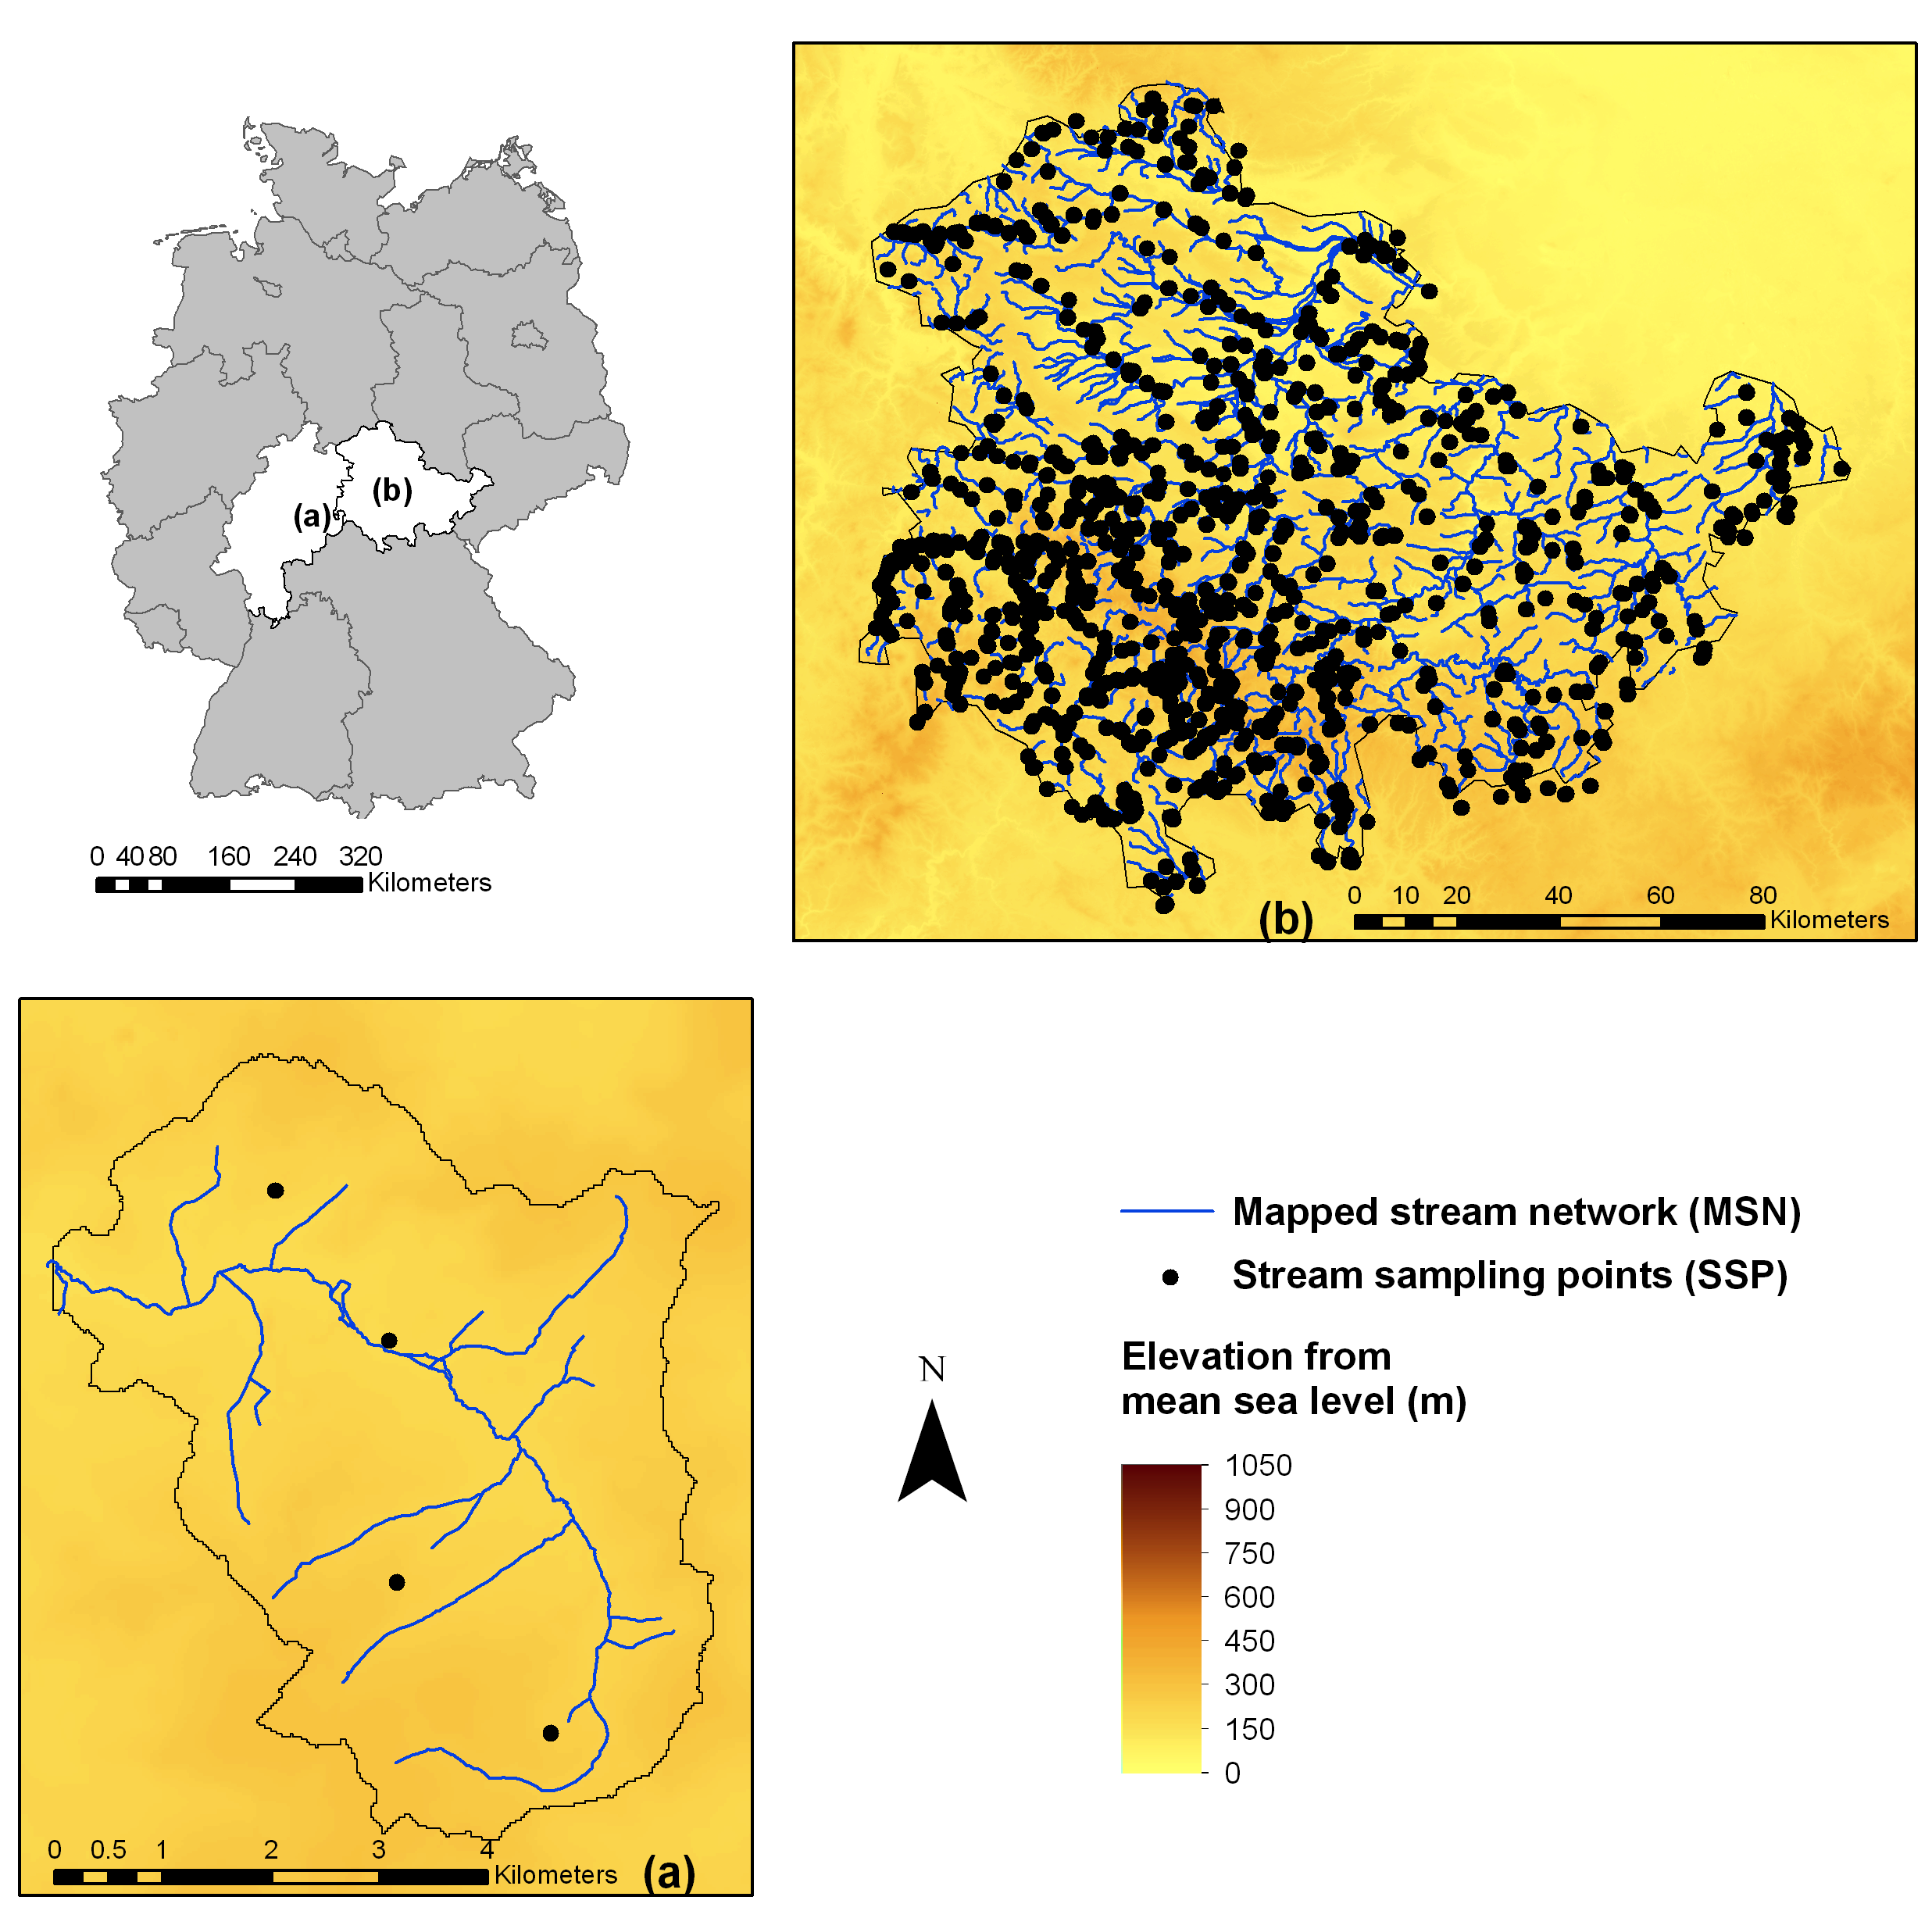
\includegraphics[width=\textwidth]{Figures/Fig_2_1.png}
  \caption{The digital elevation models (DEM) (in the background), mapped stream networks (MSN) and stream sampling points (SSP) in the (a)  watershed at  northeast of German state Hessen and (b) German state Thüringen. The inset represents the included states on a German administrative map. Details of the spatial reference system: coordinate system- Gauss Krüger, projection- Transverse Mercator, datum- Deutsches Hauptdreiecksnetz and units- Meter. Data source: HMUELV (2013), NASA and METI (2009) and TMLFUN (2013).}
  \label{Fig_2_1}
\end{figure}

ATRIC was implemented using R (R Core Team, 2014) with an interface to GRASS GIS (GRASS Development Team, 2014), i.e. the package “spgrass6” that allows for running GRASS GIS modules from the R environment (Bivand, 2007). The other used R packages were- “raster” (Hijmans and Van Etten, 2010), “rgdal” (Keitt et al., 2010), “maptools” (Lewin-Koh et al., 2011) and “rgeos” (Bivand and Rundel, 2012). The used GRASS GIS modules were- “r.watershed” (Metz et al., 2011), “r.stream” (Jasiewicz and Metz, 2011), “r.water.outlet”(Lagacherie et al., 2010), “v.net”, “v.distance” and “v.overlay” (Hofierka et al., 2009).

\subsection{Automated accumulation threshold selection}
\label{Automated accumulation threshold selection}

\subsubsection{Flow accumulation raster computation}
\label{Flow accumulation raster computation}

The automated accumulation threshold (AT) selection method is outlined in Figure 2.2 and electronic supplementary material (ESM) A.1, L 51-434 (see appendix A for details). The mapped stream network (MSN) was rasterized. A flow direction raster was computed from the digital elevation model (DEM) with the integrated single flow direction (D8) algorithm (Jenson and Domingue, 1988). However, ATRIC could also be used for the multiple flow direction (FD8) algorithm (Quinn et al., 1991). The D8 was preferred over the FD8 algorithm as it yielded better results in previous studies together with a more accurate representation of the actual stream flows on earth surface (Wolock and McCabe, 1995). Hereafter, the flow direction raster was used as input for a flow accumulation raster computation from the DEM (Metz et al., 2011).

\subsubsection{Mapped single segment node identification}
\label{Mapped single segment node identification}

The points on segments of a stream network that represent sources, outlets, meets (confluence) and crisscrosses of flowing water are called “nodes”. Thus, a node can be connected to single (source and outlet nodes) or multiple stream segment(s) (confluence and crisscross nodes). The nodes in the mapped stream network (MSN) were extracted and the number of stream segments that were connected to each of the nodes was evaluated. Then the nodes with a single segment (sources or outlets) were identified and named as “mapped single segment nodes”. To identify whether they are sources or outlets, the extracted mapped single segment nodes were grouped to exhibit connecting paths for water-flow (Metz et al., 2011; ESM A.1, L 189-199). Each group contained one outlet node that was connected to single or multiple source node(s), i.e. water could flow from the source(s) to the outlet through the connecting path (see the workflow of “v.net.components” (Hofierka et al., 2009) and ESM A.1, L 201-214).

\subsubsection{Lateral displacement selection}
\label{Lateral displacement selection}

An accumulation threshold (AT) is commonly measured as the mean of accumulations at stream sources (stream start nodes) (Heine et al., 2004; Jasiewicz and Metz, 2011; Lin et al., 2006). To extract the accumulations at sources of the digital elevation model (DEM)-derived stream network (DSN), first the location of single segment nodes of DSNs were identified and corresponding accumulations were extracted from the flow accumulation raster. The flow accumulation raster and previously identified mapped single segment nodes were overlaid for this purpose. Our AT selection method relies on the assumption that sources of DSNs should be located within a distance $d$ from the sources of mapped stream networks (MSN), which represents the lateral displacement between DSNs and MSNs. Considering this potential lateral displacements ($d$), circular buffers of varying $d$s were created around the mapped single segment nodes to search for accumulations. The initial $d$ was set two-fold the DEM resolution, i.e. 50 m, and was consecutively increased by the same (50 m) in a repeat loop for conducting the following three steps for each $d$:

\begin{enumerate}[(i)]

\item The cells with highest accumulations located within the $d$s around the mapped single segment nodes in each group were extracted along with their accumulation values, as stream cells have higher accumulations than surrounding cells (see Figure 2.2(a), step 1 and Jasiewicz and Metz, 2011). The center of these cells were the corresponding single segment nodes of DSNs for the varying $d$s (ESM A.1, L 216-331).

\noindent\begin{figure}[h!]
  \centering
  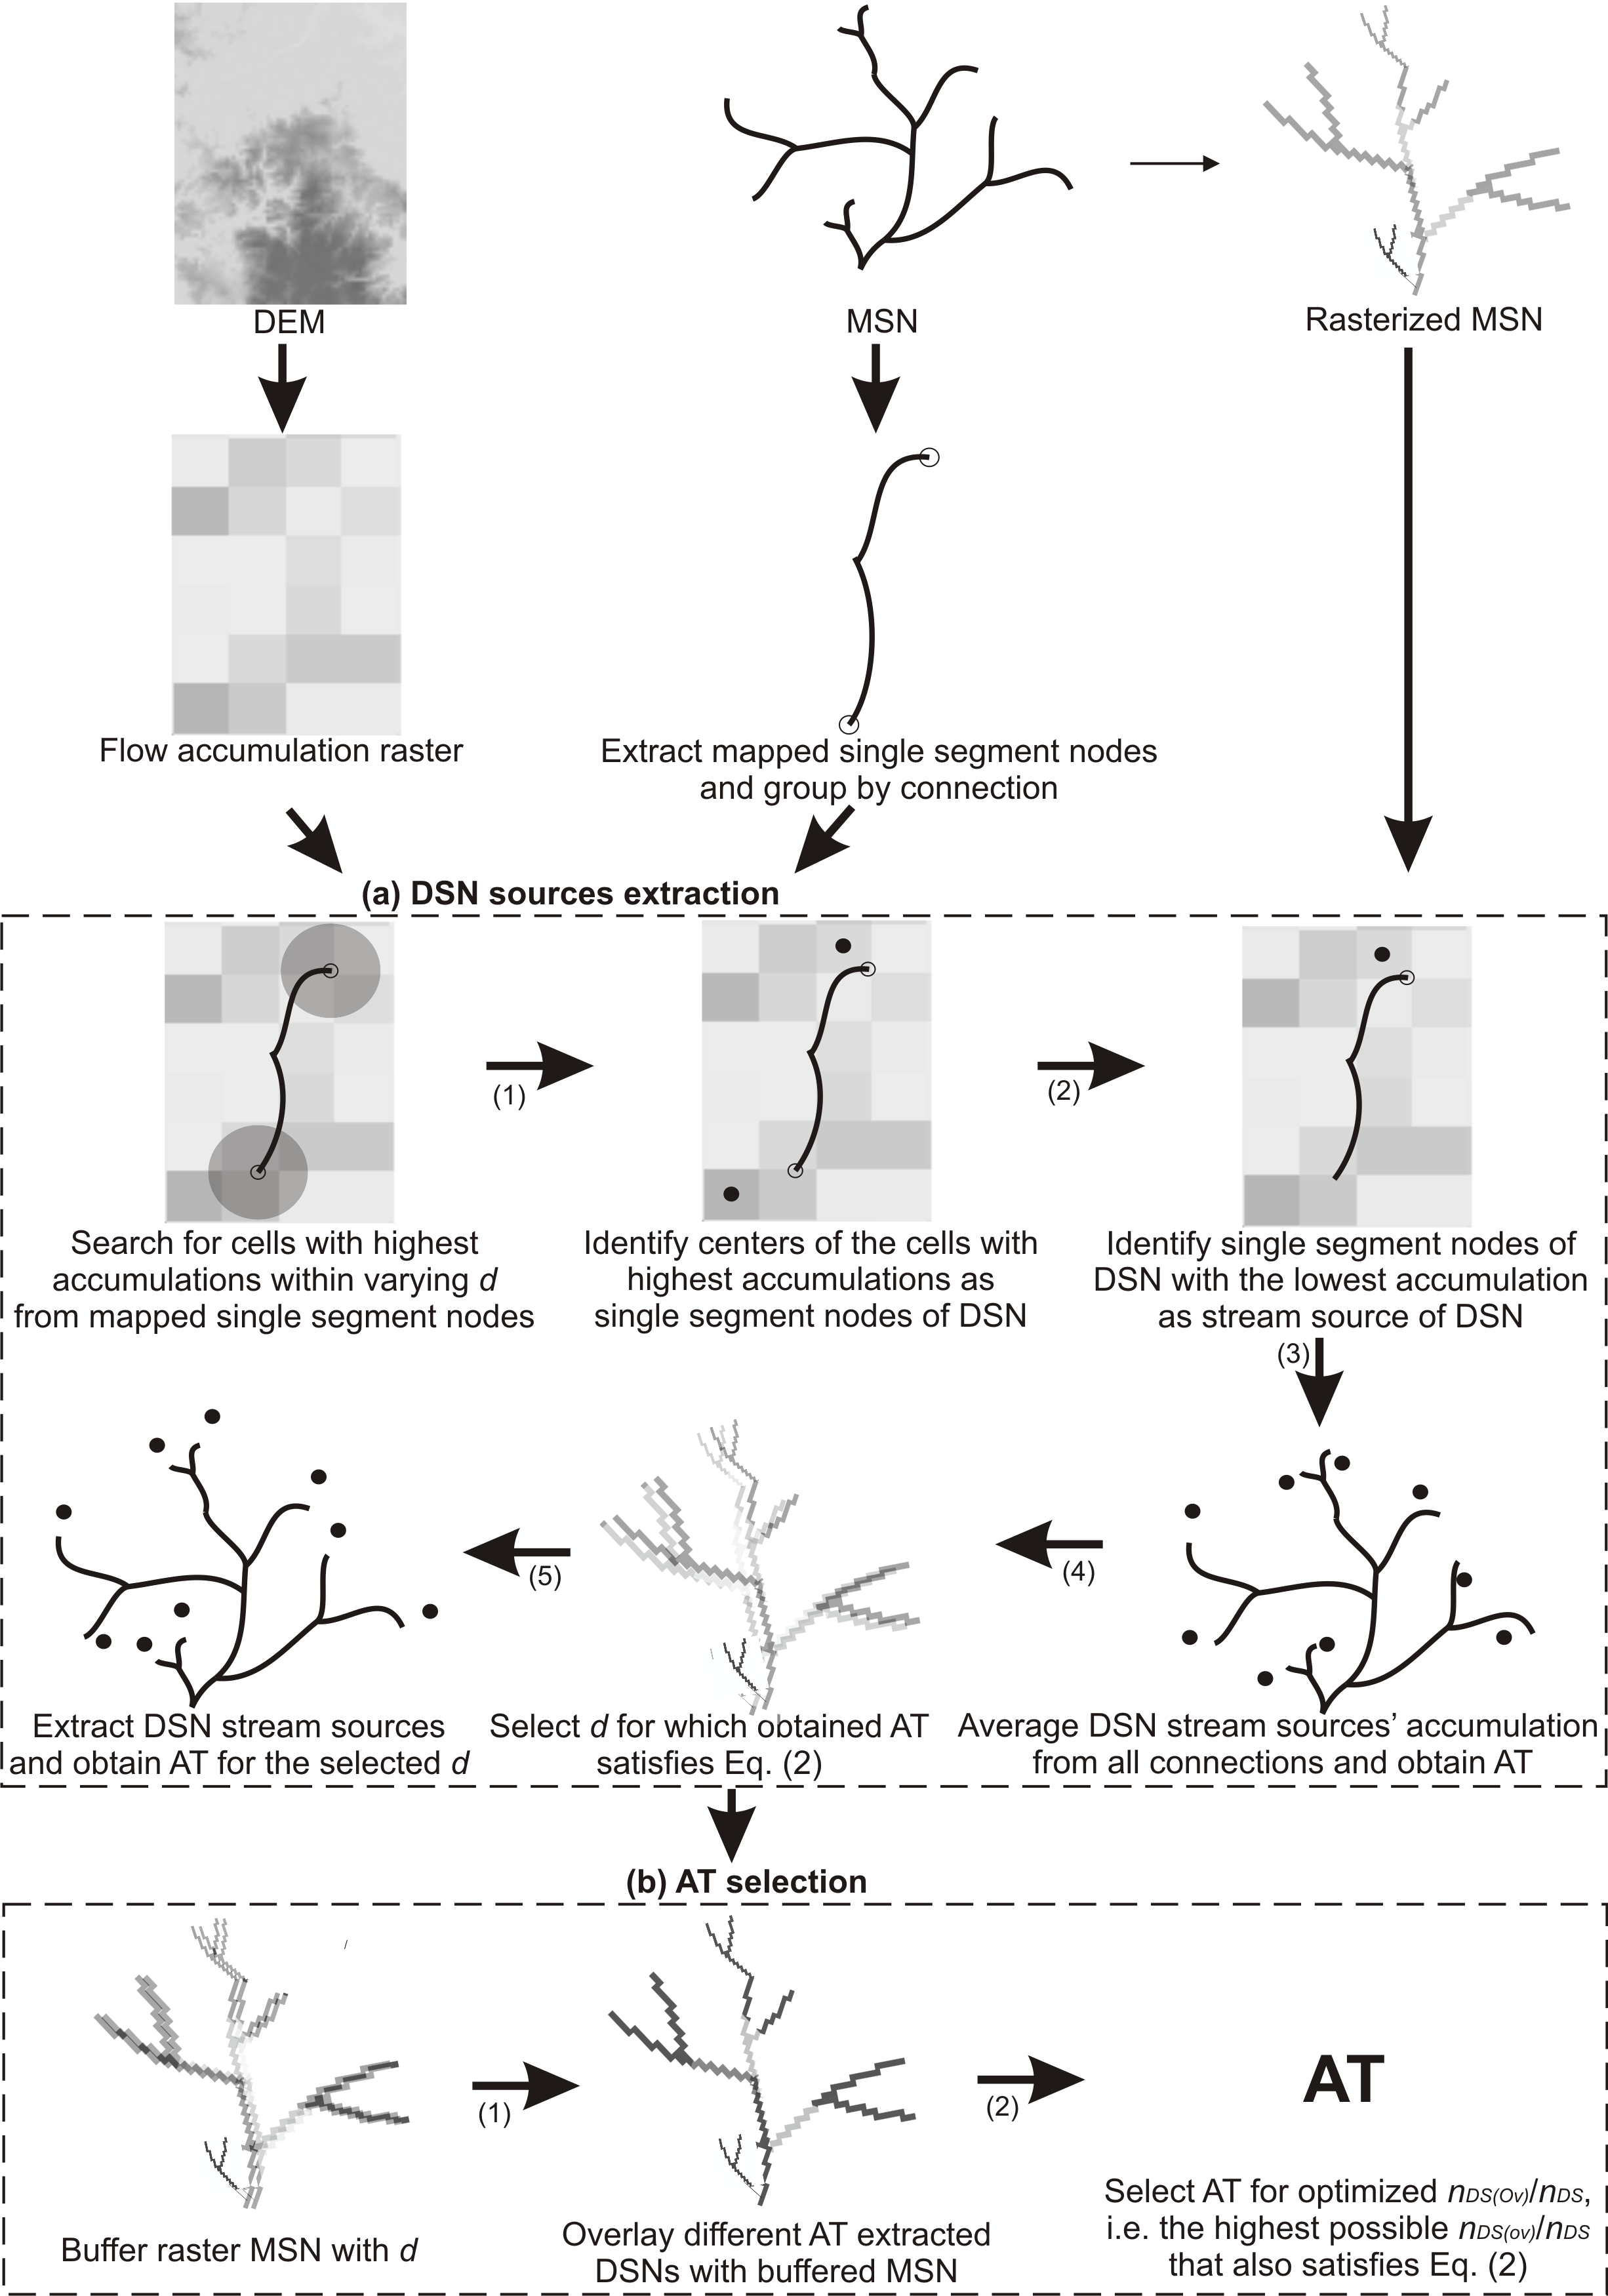
\includegraphics[width=0.8\textwidth]{Figures/Fig_2_2.png}
  \caption{The work flow of the automated accumulation threshold selection method. The used abbreviations (order: left to right and then top to bottom) – DEM: digital elevation model, MSN: mapped stream network, DSN: DEM-derived  stream network, $d$: lateral displacement between DSN and MSN, AT: accumulation threshold, $n_{DS(ov)}$: number of overlapped DEM stream cells with the selected $d$ buffered mapped stream cells and $n_{DS}$: number of DEM stream cells. The numbers below the arrows indicates the corresponding processing step.}
  \label{Fig_2_2}
\end{figure}\vspace{-0.5cm}

\item Corresponding stream sources of DSNs were identified from each group of single segment nodes of DSNs based on the lowest cell accumulations (accumulation at sources are lower than at outlets and vice versa) for the varying $d$s (see Figure 2.2(a), step 2). Then, for each $d$, an AT was computed as the mean of the accumulations at stream sources on the DEM from all groups. However, considering differences in scales and study objectives of users, the 5\textsuperscript{th}, 50\textsuperscript{th} and 95\textsuperscript{th} percentile values (can be changed by users according to their needs) of the accumulations at sources were also provided. The distributions of the AT values at stream sources of DSNs for the Hessen watershed and state Thüringen are provided in Figure A.1 in appendix A. Finally, a DSN was extracted using the AT for each of the $d$s (see Figure 2.2(a), step 3-4 and ESM A.1, 216-331).

\item The extracted number of streams ($n_{DS}$) of DSNs is an inverse function of AT, i.e. a lower AT extracts higher number of streams and vice-versa (Montgomery and Foufoula-Georgiou, 1993). Moreover, the AT increases with the width of search buffer $d$ around sources of MSNs (Figure A.2 in appendix A). Given the expected lateral displacements between the MSN and DSN, a search with a lower than optimal $d$ (Figure A.2(a)) would not include the source of the corresponding DSN and consequently yield a lower than optimal AT. By contrast, a search with a higher than optimal $d$ (Figure A.2(b)) would include non-source DSN cells and result in a higher than optimal AT. From this follows that $n_{DS}$ is an inverse function of $d$ (Eq. 2.1).

\begin{equation}
n_{DS(opt.)}=f(\frac{1}{d})
\label{Eq. 2.1}
\end{equation}

The extracted $n_{DS}$ was compared to the number of mapped stream cells ($n_{MS}$) for all $d$s and then optimized ($n_{DS(opt.)}$) by using Eq. (2).

\begin{equation}
n_{DS}=n_{MS}+min(n_{DS}-n_{MS});with\frac{n_{DS}-n_{MS}}{n_{MS}}<0.05
\label{Eq. 1.1}
\end{equation}

The term min($n_{DS} – n_{MS}$) indicates the minimum of the difference between the number of DSN and MSN stream cells. The $n_{DS}$ was constrained to be a maximum of 5\% higher than the $n_{MS}$ (as indicated by the constraints: with ($n_{DS} – n_{MS})/n_{MS}<0.05$) to assure that all streams of the MSN were extracted from the DEM and while minimizing the extraction of non-existing streams (Figure 2.2(a)).

\end{enumerate}

The $d$ that extracted $n_{DS(opt.)}$ was selected as the lateral displacement between the MSN and DSN. To increase precision, from this step $d$ was further consecutively decreased by 10 m (1/5th of the initial $d$) in the loop and the lateral displacement was selected satisfying Eq. (2). However, the initial $d$ as well as the values for the increase and decrease can be chosen by users according to their requirements regarding precision and scale of the project. The corresponding accumulation threshold for the selected lateral displacement $d$ ($AT_d$) was selected for further processing.

\subsubsection{Overlap optimization between mapped and DEM-derived streams}
\label{Overlap optimization between mapped and DEM-derived streams}

First, the mapped stream network (MSN) was buffered with the selected lateral displacement ($d$) and then overlaid with the digital elevation model (DEM)-derived stream networks (DSN) extracted for different accumulation thresholds (AT). Subsequently, the percentage of overlapped DEM-derived stream cells ($n_{DS(ov)}/n_{DS}$) was computed (see Figure 2.2(b), step 1 and ESM A.1, L 333-413). The initial AT was the one for the selected $d$ ($AT_d$) and was consecutively increased or decreased by $10^{n-1}$ unit, where $10{n-1}<AT_d\leq 10^n; n \in N$, to increase $n_{DS(ov)}/n_{DS}$. For example, the increments or decrements were 100 and 1000 for the ATds of 370 (Hessen watershed, $10<370\leq 1000$) and 8543 (Thüringen, $1000<8543\leq 10000$), respectively (see Figure 2.2(b), step 2). The highest value of the $n_{DS(ov)}/n_{DS}$ that also satisfied Eq. (2) was considered as optimal, i.e. the highest possible overlap between the MSN and DSN that also extracts all the streams of MSN from the DEM and thus minimizes non-existing streams (see Figure 2.2(b), step 2 and ESM A.1, L 333-413). To enhance precision, the optimization of AT was continued with $10^{n-2}$unit (ignored when n=1) increase or decrease until it also yielded the highest overlap that satisfied Eq. (2). The corresponding AT for the optimized $n_{DS(ov)}/n_{DS}$ was regarded as the optimal AT for comparable DSN extraction. This AT was then employed for the extraction of the DSN from previously computed flow accumulation raster (ESM A.1, L 414-417). The $n_{DS(opt.)}$ and optimized $n_{DS(ov)}/n_{DS}$  represent the goodness-of-fit measures for the DSN.

\subsection{Automated upstream riparian corridor delineation}
\label{Automated upstream riparian corridor delineation}

The automated upstream riparian corridor (URC) delineation method is outlined in Figure 2.3 and ESM A.1, L 438-590. First, upstream catchments (UC) were delineated for the given stream sampling points (SSP) (Lagacherie et al., 2010). The delineation of UCs for the original SSP data was impeded by substantial lateral displacements from mapped stream networks (MSN) (Figure A.3 in appendix A). Therefore SSPs were first snapped to the  MSN by matching their corresponding stream names (see Figure 2.3(a), step 1). Nonetheless, users may also snap SSP to MSN by shortest euclidean distance if stream names are not available . Thereafter, previously snapped SSPs were snapped to the approximate DSN by shortest euclidean distance. If the DSN is extracted without comparing to a MSN (integration with other tools for automated AT extraction (Montgomery and Foufoula-Georgiou, 1993; Tarboton, 2005) or no MSN is available), the SSPs could be directly snapped to the DSN by shortest euclidean distance, as suggested by (Tarboton, 2005).

The length and width of the URCs were set to 10 km and 100 m, respectively, as these parameters are frequently used in freshwater research (though can be changed by users according to their study objectives) (Lorenz and Feld, 2013). However, the algorithm could also be integrated with other tools for delineating riparian corridors based on geomorphology and stream side characteristics (Abood et al., 2012; Fernández et al., 2012; Holmes and Goebel, 2011), allowing for the delineation of URCs of variable lengths and widths. Stream sections of the defined length were extracted from all stream segments that were connected to SSPs as upstream segments were unknown. This also included extracting junctions and bifurcations of stream sections. These stream sections were buffered by the defined width (see Figure 2.3(b), step 1). Then the buffered stream sections were masked by the previously extracted UCs yielding to the final URCs (see Figure 2.3(b), step 2 and ESM A.1, L 532-579). In case of integration with other tools, delineated riparian corridors for stream and stream sections by those tools need to be masked by the UCs to delineate URCs of variable sizes for given SSPs.

The complete R script for the analyses that is provided as the electronic supplementary materials (ESM) A.1 contains detailed commentary on each step. To allow for reproducibility, the required DEM, MSN and SSP data are also made available in an online repository:

\noindent \href{http://doi.pangaea.de/10.1594/PANGAEA.825001}{http://doi.pangaea.de/10.1594/PANGAEA.825001}.

\subsection{Comparison with other algorithms}
\label{Comparison with other algorithms}

ATRIC was compared with the available two algorithms (Heine et al., 2004; Lin et al., 2006) that automated the accumulation threshold (AT) selection process through a similar approach, i.e. comparison with mapped stream networks (MSN). The equivalent goodness-of-fit measures for the digital elevation model (DEM)-derived stream networks (DSN), i.e. percentage of “error stream length” in Heine et al. (2004) and “overlaid coincidental stream links” in Lin et al. (2006), were obtained and adjusted, i.e. “100-percentage of error stream length” for Heine et al. (2004). Hereafter, these measures were compared to the goodness-of-fit measure of ATRIC, i.e. percentage of overlapped stream cells with buffered mapped streams ($n_{DS(ov)}/n_{DS}$). Simultaneously, the corresponding spatial scales (extents) of the study areas were also compared.

\section{Results and Discussion}
\label{Results and Discussion}

\subsection{Automated accumulation threshold and spatial scale}
\label{Automated accumulation threshold and spatial scale}

In this paper, we developed ATRIC that extracted stream networks (DSN) from digital elevation

\noindent\begin{figure}[h!]
  \centering
  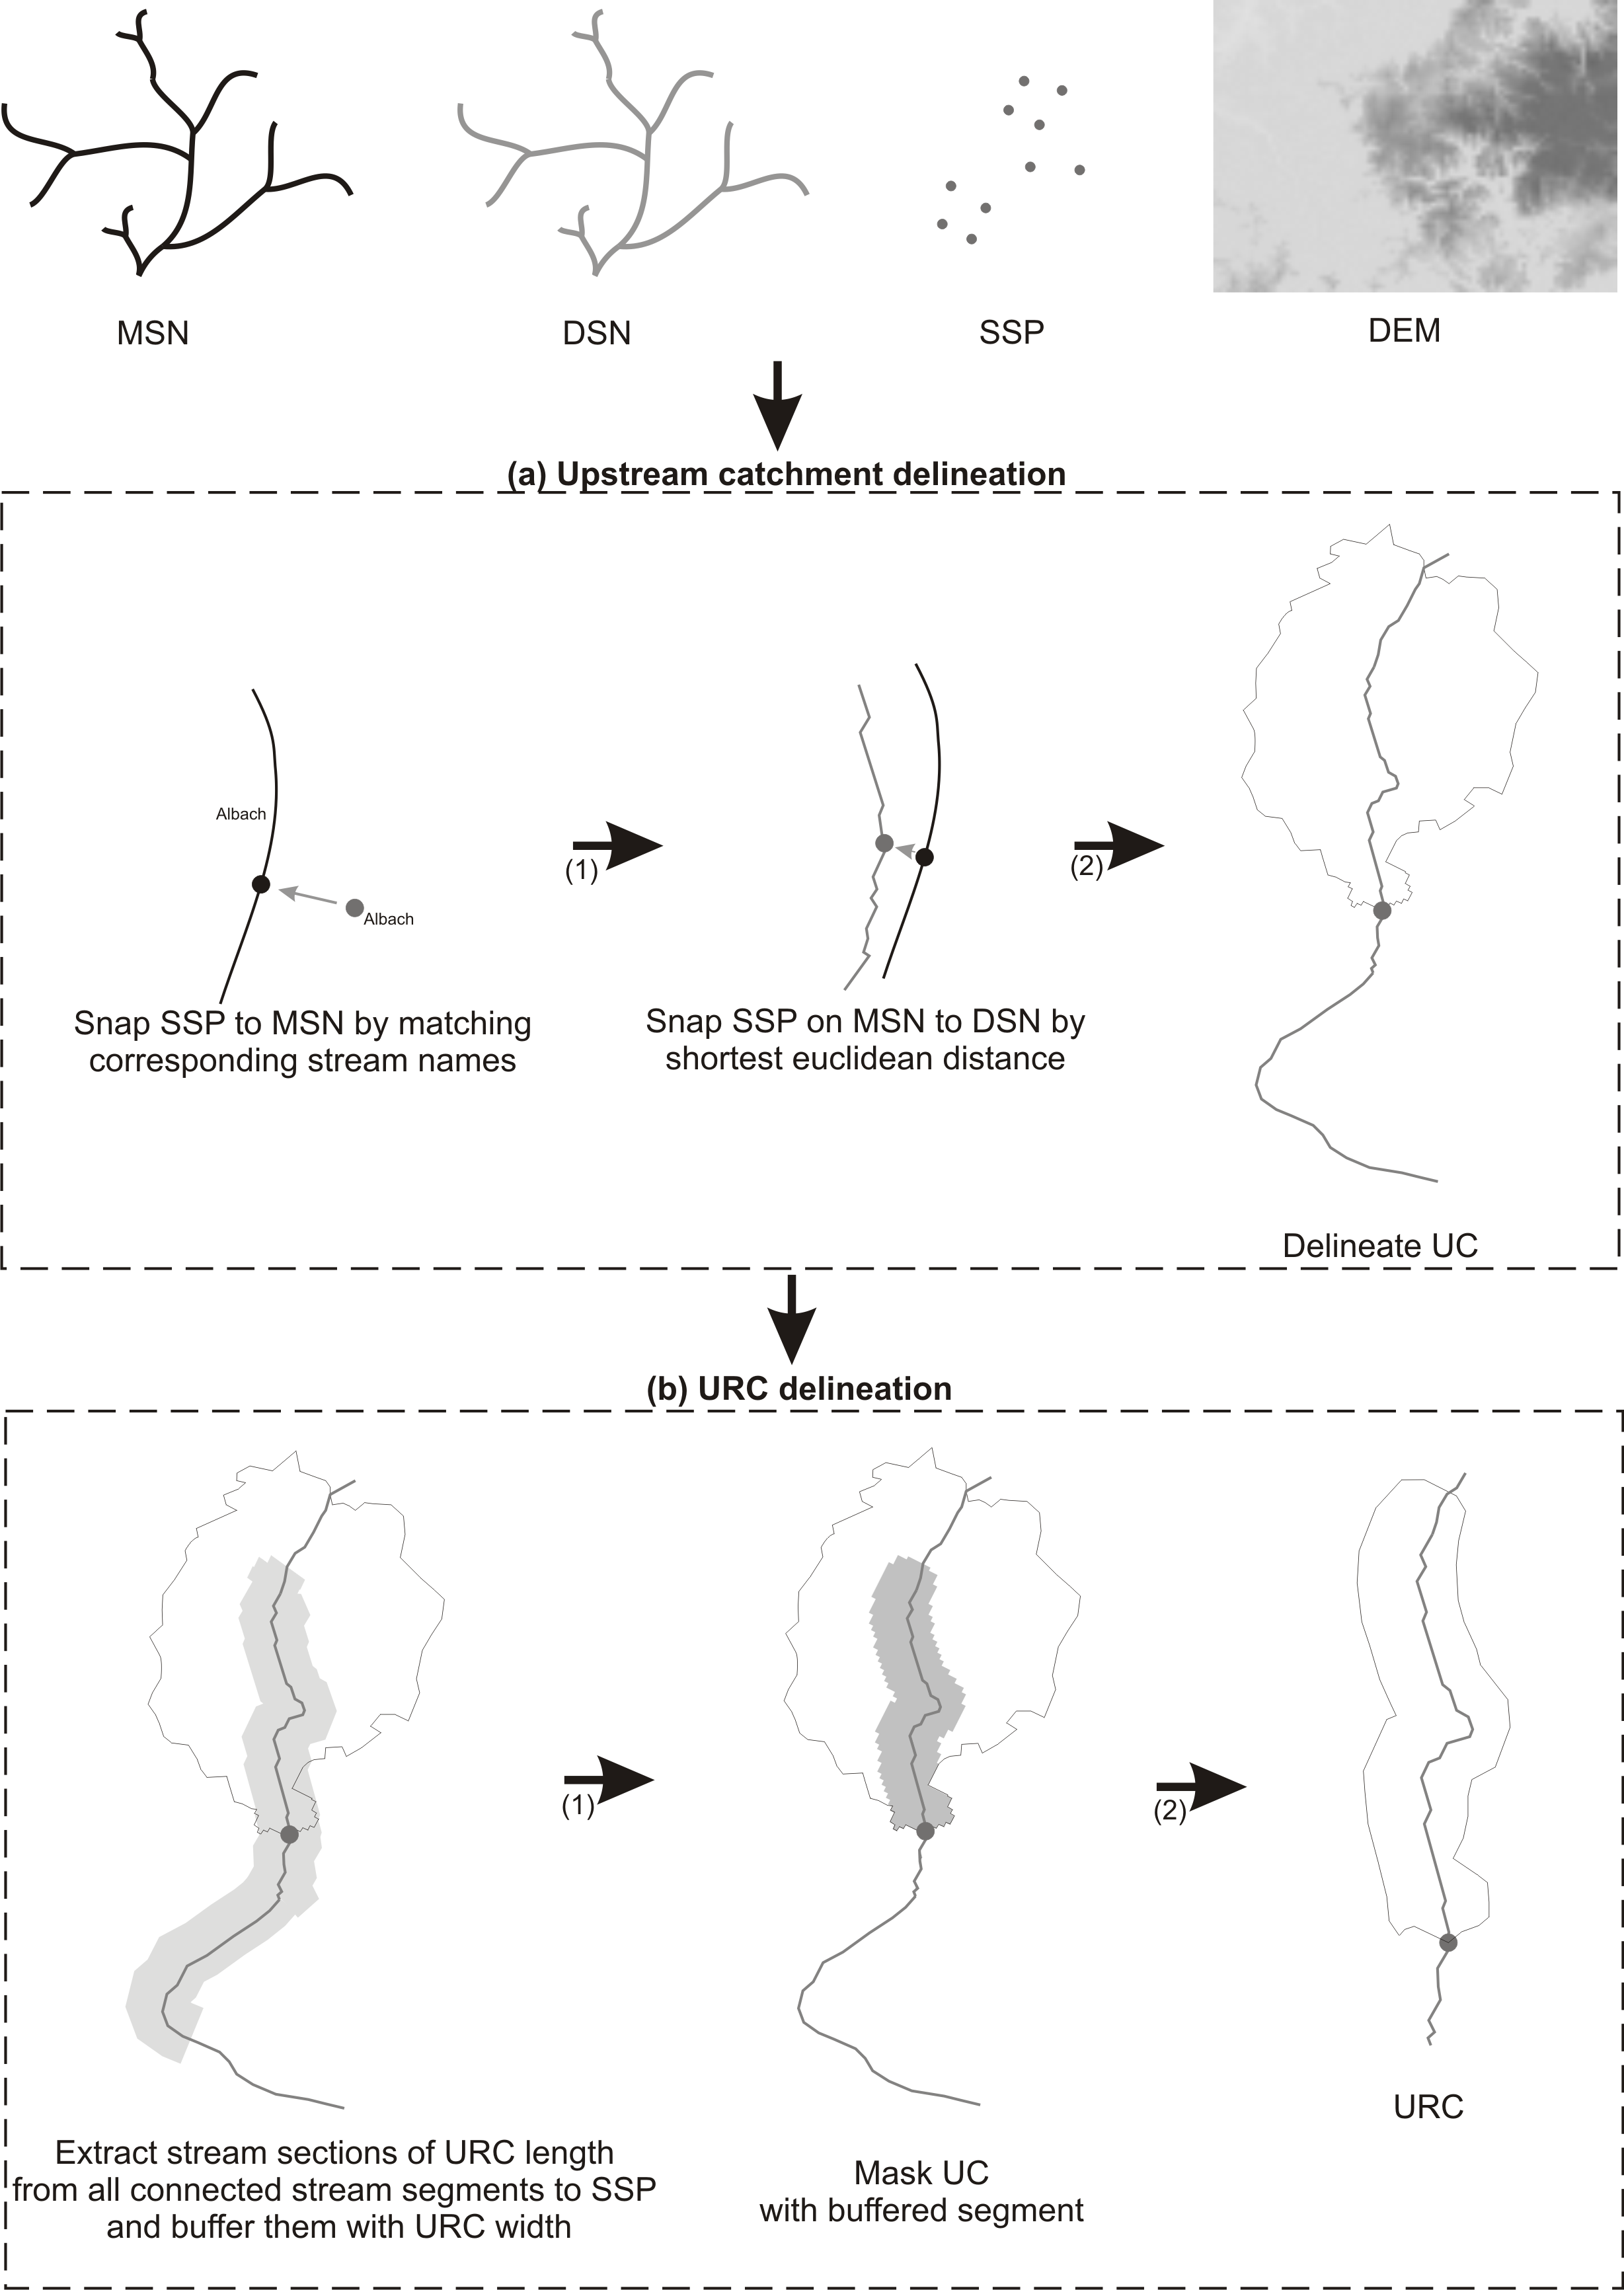
\includegraphics[width=0.8\textwidth]{Figures/Fig_2_3.png}
  \caption{The work flow of the upstream riparian corridor delineation method for given stream sampling points. The used abbreviations (order: left to right and then top to bottom) – MSN: mapped stream network, DSN: digital elevation model (DEM)-derived stream network,  SSP: stream sampling points and URC: upstream riparian corridor. The numbers below the arrows indicates the corresponding processing step.}
  \label{Fig_2_3}
\end{figure}

\noindent models (DEM) using automatically selected accumulation thresholds (AT) that maximize concordance with traditionally mapped stream networks (MSN). The tool was applied on two different spatial scales (extents), given that spatial scale impacts on the selection of an AT (Murphy et al., 2008). Large scale studies require DSNs of high stream orders, e.g. in large watersheds, corresponding to the selection of a high AT. Conversely, small scale studies often focus on lower stream order and dense DSNs corresponding to the selection of a low AT. However, ATRIC automatically adjusts to the scale of the provided MSNs and selects an AT on the related scale conditional that the resolution of the used DEMs is appropriate. For example, a small scale study that requires a dense stream network should apply DEM with a sufficiently high resolution, whereas a coarse-resolution DEM might suffice for a large scale study. Overall, users of ATRIC should select DEMs with appropriate resolution with respect to the order and density of MSNs.

\subsection{Goodness of stream network extraction from digital elevation models}
\label{Goodness of stream network extraction from digital elevation models}

The digital elevation model (DEM)-derived stream networks (DSN) extracted by ATRIC exhibited good agreement with the mapped stream networks (MSN) on both spatial scales (Table 2.1 and 2.2; Figure 2.4). The AT obtained from the automatically selected $d$ ($AT_d$, 370 and 8543) for the Hessen watershed and state Thüringen extracted almost equivalent (2.93\% and 4.77\% higher) number of DSN ($n_{DS}$) compared to the number of MSN stream cells ($n_{MS}$) (Table 2.1). The ATs (500 and 9543) obtained from the further optimization of the $AT_d$s were marginally different from the $AT_d$s but considerably improved the concordance between the $n_{DS}$ and $n_{MS}$, i.e. obtained $n_{DS}$s were only 0.24\% and 0.43\% higher than the $n_{MS}$s for the Hessen watershed and state Thüringen, respectively (Table 2.2). Moreover, the extracted DSNs entailed high (89.36\%) and moderate (57.42\%) overlaps with the MSNs buffered with the selected $d$s for the Hessen watershed and state Thüringen, respectively (Table 2.2).

When compared to the goodness-of-fit of other algorithms on comparative spatial scales, ATRIC showed similar or better performance (Table 2.3). The spatial extent of the Hessen watershed is 75 times larger and 1.6 times smaller on average than the watersheds used in Heine et al. (2004) and Lin et al. (2006), respectively. Nevertheless, while compared to Heine et al. (2004) and Lin et al. (2006), the goodness-of-fit of the extracted DSN for the Hessen watershed was higher. However, the goodness-of-fit of the extracted DSN for the state Thüringen was lower where the spatial extent

\noindent\begin{table}[h!]
\label{Table 2.1}
\caption{The results of number of digital elevation model (DEM)-derived stream cells ($n_{DS}$) optimization to obtain average lateral displacements ($d$) between mapped stream network (MSN) and DEM-derived stream network (DSN). The computed accumulation threshold (AT), $n_{DS}$ and the percentage high or low are the $n_{DS}$ from the number of mapped stream cells ($n_{MS}$), i.e. (($n_{DS}-n_{MS})/n_{MS}$) are reported with varying $d$s.}
\begin{threeparttable}
\centering
\begin{tabular}{>{\centering\arraybackslash}m{2.6cm}>{\centering\arraybackslash}m{1.5cm}>{\centering\arraybackslash}m{3cm}>{\centering\arraybackslash}m{2.5cm}>{\centering\arraybackslash}m{0.7cm}>{\centering\arraybackslash}m{1.3cm}}

\toprule
\textbf{Spatial scale} & \textbf{Variable $d$} & \textbf{Consecutive increase or decrease in the $d$} & \textbf{Computed AT} & \textbf{$n_{DS}$} & \textbf{$\frac{n_{DS} - n_{MS}}{n_{MS}}$}\\
 & \textbf{$(m)$} & \textbf{$(+/- m)$} & & & \textbf{$(+/- \%)$}\\

\midrule

 & 50 & - & 55 & 3469 & +182.49\\
 & 100 & +50 & 263 & 1734 & +41.21\\
 & 150 & +50 & 362 & 1325 & +7.89\\
Hessen watershed & 200 & +50 & 654 & 1086 & -11.56\\
 & 190 & -10 & 652 & 1088 & -7.00\\
 & 180 & -10 & 592 & 1142 & -7.00\\
 & 170 & -10 & 572 & 1167 & -4.97\\
 &
 \rowcolor{Gray}
 160 & -10 & 370 & 1264 & +2.93\\
\hline
 & 50 & - & 279 & 986647 & +391.92\\
 & 100 & +50 & 1717 & 442971 & +120.85\\
Thüringen state & 150 & +50 & 9756 & 199451 & -0.56\\
 &
 \rowcolor{Gray}
 140 & -10 & 8543 & 210133 & +4.77\\
 & 130 & -10 & 8485 & 212799 & +6.09\\

\bottomrule

\end{tabular}
\begin{tablenotes}
\footnotesize
\colorbox{Gray}{Grey highlighted} = The obtained $d$ between $DSN$ and $MSN$ by $n_{DS}$ optimization, corresponding $AT (AT_d)$ and $\frac{n_{DS} – n_{MS}}{n_{MS}}$ 
\end{tablenotes}
\end{threeparttable}
\end{table}

\newpage

\noindent\begin{table}[t!]
\label{Table 2.2}
\caption{The results of overlapped digital elevation model (DEM)-derived stream cells ($n_{DS(ov)}$) with buffered mapped stream cells optimization to select an accumulation threshold (AT). The percentages of overlapped DEM-derived stream cells ($n_{DS(ov)}/n_{DS}$) with varying ATs are reported.}
\centering
\begin{threeparttable}
\begin{tabular}{>{\centering\arraybackslash}m{2.6cm}>{\centering\arraybackslash}m{1.5cm}>{\centering\arraybackslash}m{4cm}>{\centering\arraybackslash}m{1.5cm}>{\centering\arraybackslash}m{1.5cm}}

\toprule
\textbf{Spatial scale} & \textbf{AT} & \textbf{Consecutive increase or decrease in the AT starting from the $AT_d$ (Table 2.1)} & $\frac{n_{DS}(ov)}{n_{DS}}$ & $\frac{n_{DS} - n_{MS}}{n_{MS}}$\\
 & & $+/- unit$ & $(\%)$ & (+/- \%)\\

\midrule

 & 370 & - & 83.15 & +2.93\\
 & 470 & +100 & 88.53 & +2.06\\
 Hessen watershed & 480 & +10 & 88.90 & +1.22\\
 & 490 & +10 & 89.32 & +0.65\\
 &
 \rowcolor{Gray}
 500 & +10 & 89.36 & +0.24\\
 & 510 & +10 & 90.06 & -0.90\\
\hline
 & 8593 & - & 56.06 & +4.77\\
Thüringen state &
\rowcolor{Gray}
9543 & +1000 & 57.42 & +0.43\\
 & 9643 & +100 & 57.53 & -0.04\\
 
\bottomrule

\end{tabular}
\begin{tablenotes}
\footnotesize
\colorbox{Gray}{Grey highlighted} = The AT obtained by $n_{DS}(ov)/n_{DS}$ optimization and corresponding $\frac{n_{DS}(ov)}{n_{DS}}$ and $\frac{n_{DS} - n_{MS}}{n_{MS}}$
\end{tablenotes}
\end{threeparttable}
\end{table}

\vspace{-1.0cm}\noindent\begin{table}[h!]
\label{Table 2.3}
\caption{Comparison of the goodness-of-fit of the ATRIC extracted stream networks from the digital elevation models (DEM) with the stream networks extracted by other algorithms for automated accumulation threshold selection.}
\centering
\begin{tabular}{>{\centering\arraybackslash}m{1.5cm}>{\centering\arraybackslash}m{2.2cm}>{\centering\arraybackslash}m{1.5cm}>{\centering\arraybackslash}m{1.8cm}>{\centering\arraybackslash}m{3.5cm}>{\centering\arraybackslash}m{1.5cm}}

\toprule
\textbf{Source} & \textbf{Study area} & \textbf{Spatial extent} & \textbf{Resolution of the used DEMs} & \textbf{Comparable measure of the goodness-of-fit} & \textbf{Goodness-of-fit}\\
 & & $km^2$ & $(m)$ & & $(\%)$\\

\midrule

 Heine et al. (2004) & Tallgrass National Park watershed & 0.6 & 10 & 100 – percentage of total error stream & 87.30\\
 \hline
 \multirow{2}{1.5cm}{\centering Lin et al.(2006)} & Chi-Jia-Wang watershed & 74.03 & \multirow{2}{1.5cm}{\centering 40} & \multirow{2}{3.5cm}{\centering Percentage of overlaid coincidental stream links} & 70\\
 & Erh-Wu watershed & 51.36 & & & 72\\
 \hline
 \multirow{2}{*}{\centering ATRIC} & Hessen watershed & 45 & \multirow{2}{1.5cm}{\centering 25} & \multirow{2}{3.5cm}{\centering Percentage of overlapped stream cells with mapped streams buffered by a selected lateral displacement} & \vspace{12pt} 89.36\\[0.6cm]
 & Thüringen state & 16171 & & & \vspace{12pt} 57.42\\[0.6cm]
 
\bottomrule

\end{tabular}
\end{table}

\noindent was approximately 360 times larger than the Hessen watershed. These results are supported by Goodchild and Gopal (1989) and Murphy et al. (2008), who showed that the goodness-of-fit of GIS analyses is scale-dependent, e.g. smaller scale stream extraction results in better goodness-of-fit. Moreover, constant ATs selected on smaller spatial scales are more representative of the topography and geomorphology of study areas because of more homogeneity and hence, yield better overlap with MSNs (Heine et al., 2004; Lin et al., 2006). However, ATRIC represents an improvement in extraction precision on large scales because of optimization of the $n_{DS}$ before determining the $n_{DS(ov)}/n_{DS}$ and thus advances previous algorithms.

\noindent\begin{figure}[h!]
  \centering
  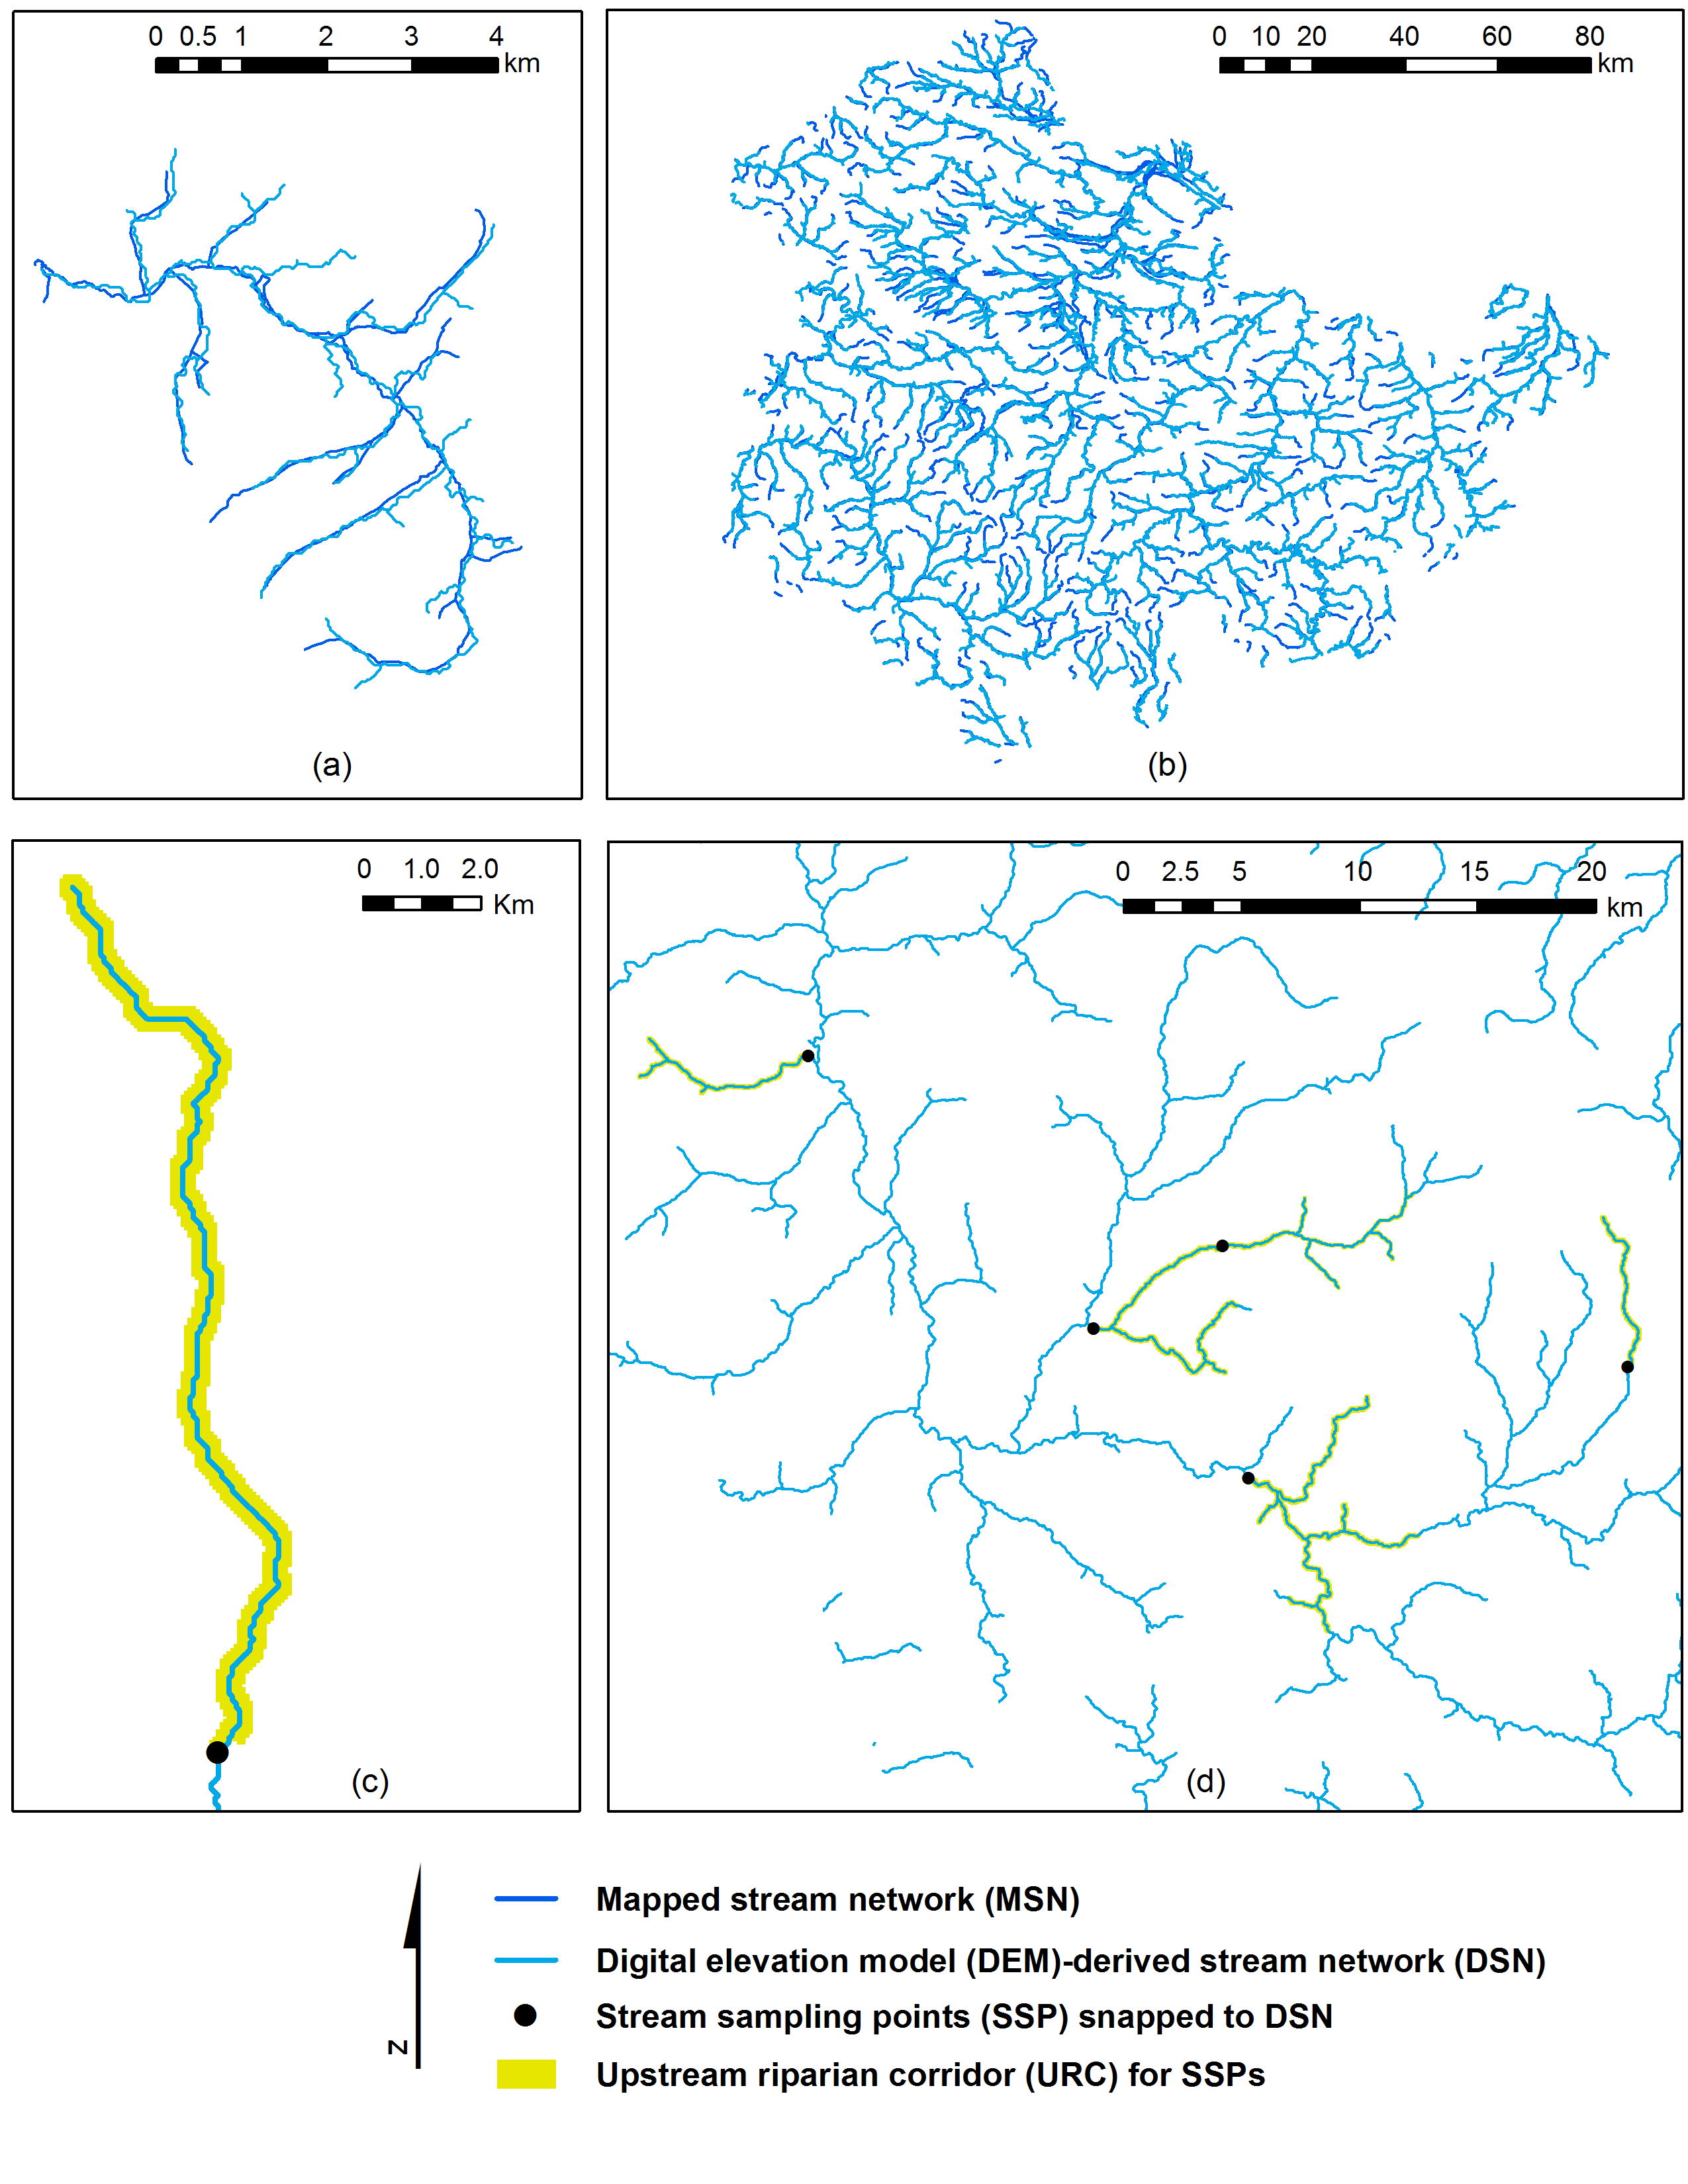
\includegraphics[width=0.785\textwidth]{Figures/Fig_2_4.png}
  \caption{The digital elevation model (DEM)-derived stream networks (DSN) by ATRIC overlaid with mapped stream networks (MSN) in (a) the watershed at the northeast of Hessen and (b) Thüringen, and delineated upstream riparain corridors (URC) of (c) one stream sampling point (SSP) in the Hessen watershed and ($d$) several SSPs in Thüringen.}
  \label{Fig_2_4}
\end{figure}

Geographic characteristics of study regions also influence the goodness of DSN (Wolock et al., 1990). The study regions reported in Heine et al. (2004) and Lin et al. (2006) were flat, simple and homogeneous whereas we applied ATRIC on relatively complex and heterogeneous regions and obtained comparable goodness of DSN.

Resolution, sources and creation methods of DEM also substantially affect the goodness of DSN (Li and Wong, 2010; McMaster, 2002; Murphy et al., 2008). Therefore goodness of ATRIC can be further improved by using a higher resolution (e.g. 10 m) and more advanced equipment derived (e.g. lidar) DEMs.

\clearpage

\vspace{-1.1cm}

\subsection{Computational efficiency}
\label{Computational efficiency}

ATRIC showed high computational efficiency in terms of required computation time and size of input datasets. We ran ATRIC on three different computers: (1) Linux OS with 3.8 GHz Quad-Core processor and 16 GB RAM, (2) Mac OS with 2.8 GHz Quad-Core processor and 12 GB RAM and (3) Windows OS with 2.9 GHz Dual-Core processor and 4 GB RAM. Required time for automated accumulation threshold (AT) selection on the small (watershed) and large (state) spatial scales on the Linux, Mac, Windows OS computers were 43 seconds, 58 seconds, two minutes and 33 minutes, 50 minutes, two hours, respectively. The time required for the upstream riparian corridor (URC) delineation per stream sampling point (SSP) was 30 seconds for Linux and Mac OS, and one minute for Windows OS, respectively. Moreover, the other available algorithms for automated AT selection (Heine et al., 2004; Lin et al., 2006; Montgomery and Foufoula-Georgiou, 1993; Tarboton, 2005) were developed on single watersheds and therefore the input digital elevation models (DEM) and mapped stream networks (MSN) that were processed were small in terms of number of cell. By contrast, ATRIC processed large input DEM and MSN in the state Thüringen that is comprised of 100 watersheds and a complex topography. Thus ATRIC showed an advantage over the available algorithms in terms of processing large datasets. This computational efficiency was entailed by the efficient raster processing capability in R and GRASS GIS (GRASS Development Team, 2014; R Core Team, 2014).

\vspace{-0.25cm}

\subsection{Development and integration}
\label{Development and integration}

ATRIC is the first algorithm that has been developed using free and open source software. The available algorithms relying on proprietary software have already shown substantial improvement in stream network mapping (Heine et al., 2004; Lin et al., 2006). Given the rapid growth in the market shares of open source GIS software packages (Neteler et al., 2012), ATRIC enables widespread usage and thus improvement in stream network mapping. Moreover, non-profit community motivation, non-proprietary hierarchical co-ordination and coherence with proprietary standards of the open source software ensure further development of ATRIC (Bonaccorsi and Rossi, 2003).

ATRIC was developed combining two different software packages (R and GRASS GIS) and thus advanced available GIS operations (Bivand, 2007). R provides platforms for co-interfacing with several other free open source (e.g. “SAGA GIS” (Brenning, 2007) by the package “RSAGA” (Brenning, 2008)) and proprietary (e.g. ArcGIS (ESRI, Redlands, 2001) by the package “RPyGeo” (Brenning, 2012)) GIS software packages. Thus ATRIC could be further integrated with other GIS software  packages. Importantly, ATRIC will facilitate the reproducibility of geoscientific research (Pebesma et al., 2012).

Moreover, ATRIC can be integrated with other algorithms for statistical and geostatistical modeling on stream network, i.e. SSN (Ver Hoef et al., 2012) and rtop (Skøien et al., 2014), and extraction of riparian corridors for streams and stream sections based on streamside characteristics and geomorphological analyses (Abood et al., 2012; Fernández et al., 2012; Holmes and Goebel, 2011). Currently, the data required for SSN is provided by STARS (Peterson and Ver Hoef, 2014) that depends on ArcGIS (proprietary software). ATRIC represents an open source alternative because it includes tools for building network topology, extracting a comparable digital elevation model (DEM)-derived stream network (DSN) for a given mapped stream network (MSN) considering the lateral displacement (instead of burning the MSN into the DEM which is done in STARS) and upstream catchment (UC) delineation for given points on streams. Delineating UC for given stream sampling points on MSN is also a primary requirement in rtop. Moreover, ATRIC can be integrated to extract upstream geomorpholocial riparian corridors of variable sizes for particular stream sampling points (SSP).

\vspace{-0.25cm}

\subsection{Potential fields of application}
\label{Potential fields of application}

Advances in computer technology and GIS software, and widespread availability of electronic maps and high resolution satellite imagery in recent decades facilitate far reaching applications for ATRIC. These include related fields of freshwater research, e.g. cartography, geomorphology, hydrology, ecology and water resources management. Some examples are:

\begin{enumerate}[(i)]

\item Improving accuracy, precision and efficiency of digital and traditional topographic mapping by providing high quality digital elevation model (DEM)-derived stream network (DSN, hydrological) data layers (Heine et al., 2004),

\item Enabling geomorphological analyses, e.g. flood modeling on DEM by providing corresponding DSN as such analyses are not possible on areal photographs or traditional paper maps (Gichamo et al., 2012),

\item Updating existing stream network maps by frequently updated and easily available DEMs (Olivera, 2001),

\item Extracting stream networks in unmapped regions (traditionally mapped stream networks (MSN) are not available) using the accumulation threshold (AT) derived from mapped regions (MSN available) by ATRIC. This is applicable when the unmapped region has an identical size and topography as well as environmental characteristics of the mapped region and the scales of the studies on two regions are the same. Moreover, as AT is assumed to correlate with different regional geomorphological and climatological parameters, such as plane curvature and precipitation  (Moore et al., 1991), the AT for unmapped regions could also be predicted based on the relationship of ATs in several mapped regions with these regional parameters, and

\item Detecting and quantifying different stressors due to landuse and climate change, surface runoff, ingredient flow in the URCs for convergent SSPs (Lorenz and Feld, 2013).

\end{enumerate}

Moreover, ATRIC overcame the problem of lateral displacements between MSN and DSN and can extract DSN sources without DEM alteration. Hence, ATRIC can be applied across different DEM with variable resolution, accuracy and precision for DSN extraction and URC delineation.

\section{Conclusions and outlook}
\label{Conclusions and outlook}

We developed ATRIC for the automation of accumulation threshold (AT) selection to enable objective stream network extraction and upstream riparian corridor (URC) delineation from digital elevation models (DEM) using open source software packages. The DEM-derived stream networks (DSN) by ATRIC represented a good approximation of the given mapped stream network (MSN). However, traditional field survey and derived MSNs often miss important stream stretches (Colson et al., 2008). This might affect the goodness of the extracted DSN when compared to ground truth as ATRIC primarily depends on the provided mapped stream cells. It might also affect reliability of the delineated URC for a given set of stream sampling points (SSP) because this delineation depends on the extracted approximate DSN. Nevertheless, the MSN provided by governmental authorities are widely accepted as the most accurate and precise ground truth. Moreover, the MSNs used here were previously validated against digital landscape models and orthophotos and hence, can be claimed to be less erroneous. In contrast to previous approaches (e.g. Heine et al. (2004) and Lin et al. (2006)), ATRIC is relatively independent of the location of mapped stream sources in AT selection and thus stream network extraction. Notwithstanding, future studies could enhance ATRIC by integrating variable AT selection in case of a complex topography. Furthermore, if high resolution satellite imageries are available, the DSN could be validated using satellite imageries in case that the provided MSN is erroneous. Finally, implementation of ATRIC as a pure GIS module, e.g. GIS package in R or GRASS GIS toolkit, to avoid co-interfacing as well as development of a graphical user interface might enhance accessibility and migration to other GIS platforms.

\openleft

\begingroup

\renewcommand{\addcontentsline}[3]{}

\begin{thebibliography}

\bibitem{} \hangindent=1cm Abood, S.A., Maclean, A.L., Mason, L.A., 2012. Modeling Riparian Zones Utilizing DEMS and Flood Height Data. Photogrammetric engineering and remote sensing 78, 259–269.

\bibitem{} \hangindent=1cm Arge, L., Chase, J.S., Halpin, P., Toma, L., Vitter, J.S., Urban, D., Wickremesinghe, R., 2003. Efficient flow computation on massive grid terrain datasets. GeoInformatica 7, 283–313.

\bibitem{} \hangindent=1cm Bastian, C.T., McLeod, D.M., Germino, M.J., Reiners, W.A., Blasko, B.J., 2002. Environmental amenities and agricultural land values: a hedonic model using geographic information systems data. Ecological Economics 40, 337–349.

\bibitem{} \hangindent=1cm Berhane, G., Walraevens, K., 2013. Geological and geotechnical constraints for urban planning and natural environment protection: a case study from Mekelle City, Northern Ethiopia. Environmental Earth Sciences 69, 783–798. doi:10.1007/s12665-012-1963-x

\bibitem{} \hangindent=1cm Biss, R., Kübler, P., Pinter, I., Braukmann, U., 2006. Leitbildbezogenes biozönotisches Bewertungsverfahren für Fließgewässer in der Bundesrepublik Deutschland -Ein erster Beitrag zur integrierten ökologischen Fließgewässerbewertung (Project report No. 298 24 777), UBA-FB 000348. Umweltforschungsplan des Bundesministeriums für Umwelt, Naturschutz und Reaktorsicherheit, Berlin.

\bibitem{} \hangindent=1cm Bivand, R., 2007. Using the R–Grass interface. OSGeo Journal 1, 36–38.

\bibitem{} \hangindent=1cm Bivand, R., Rundel, C., 2012. rgeos: Interface to Geometry Engine-Open Source (GEOS). R package version 0.2-2.

\bibitem{} \hangindent=1cm Bonaccorsi, A., Rossi, C., 2003. Why Open Source software can succeed. Research Policy 32, 1243–1258. doi:10.1016/S0048-7333(03)00051-9.

\bibitem{} \hangindent=1cm Brenning, A., 2007. RSAGA: SAGA geoprocessing and terrain analysis in R.

\bibitem{} \hangindent=1cm Brenning, A., 2012. RPyGeo: ArcGIS geoprocessing in R via Python.

\bibitem{} \hangindent=1cm Callow, J.N., Van Niel, K.P., Boggs, G.S., 2007. How does modifying a DEM to reflect known hydrology affect subsequent terrain analysis? Journal of Hydrology 332, 30–39. doi:10.1016/j.jhydrol.2006.06.020.

\bibitem{} \hangindent=1cm Colson, T., Gregory, J., Dorney, J., Russell, P., 2008. Topographic and soil maps do not accurately depict headwater stream networks. National Wetlands Newsletter 30, 25–28.

\bibitem{} \hangindent=1cm Dahm, V., Hering, D., Nemitz, D., Graf, W., Schmidt-Kloiber, A., Leitner, P., Melcher, A., Feld, C.K., 2013. Effects of physico-chemistry, land use and hydromorphology on three riverine organism groups: a comparative analysis with monitoring data from Germany and Austria. Hydrobiologia 704, 389–415. doi:10.1007/s10750-012-1431-3.

\bibitem{} \hangindent=1cm Danner, A., Mølhave, T., Yi, K., Agarwal, P.K., Arge, L., Mitasova, H., 2007. TerraStream: from elevation data to watershed hierarchies, in: Proceedings of the 15th Annual ACM International Symposium on Advances in Geographic Information Systems. pp. 28–35.

\bibitem{} \hangindent=1cm DeVantier, B.A., Feldman, A.D., 1993. Review of GIS applications in hydrologic modeling. Journal of Water Resources Planning and Management 119, 246–261.

\bibitem{} \hangindent=1cm Di Luzio, M., Srinivasan, R., Arnold, J.G., 2004. A GIS-Coupled Hydrological Model System for the Watershed Assessment of Agricultural Nonpoint and Point Sources of Pollution. Transactions in GIS 8, 113–136. doi:10.1111/j.1467-9671.2004.00170.x.

\bibitem{} \hangindent=1cm Environmental Systems Research Institute (ESRI), Redlands, 2001. What is ArcGIS?: GIS by ESRI. ESRI.

\bibitem{} \hangindent=1cm Fernández, D., Barquín, J., Álvarez-Cabria, M., Peñas, F.J., 2012. Quantifying the performance of automated GIS-based geomorphological approaches for riparian zone delineation using digital elevation models. Hydrology and Earth System Sciences 16, 3851–3862. doi:10.5194/hess-16-3851-2012.

\bibitem{} \hangindent=1cm Forman, R.T.T., 2003. Road ecology: science and solutions. Island Press, Washington, DC.

\bibitem{} \hangindent=1cm Garbrecht, J., Martz, L.W., 1997. The assignment of drainage direction over flat surfaces in raster digital elevation models. Journal of Hydrology 193, 204–213.

\bibitem{} \hangindent=1cm Gichamo, T.Z., Popescu, I., Jonoski, A., Solomatine, D., 2012. River cross-section extraction from the ASTER global DEM for flood modeling. Environmental Modelling & Software 31, 37–46. doi:10.1016/j.envsoft.2011.12.003.

\bibitem{} \hangindent=1cm Goodchild, M.F., Gopal, S., 1989. The Accuracy Of Spatial Databases. CRC Press.

\bibitem{} \hangindent=1cm GRASS Development Team, 2014. Geographic Resources Analysis Support System (GRASS). Open Source Geospatial Foundation Project.

\bibitem{} \hangindent=1cm Heine, R.A., Lant, C.L., Sengupta, R.R., 2004. Development and Comparison of Approaches for Automated Mapping of Stream Channel Networks. Annals of the Association of American Geographers 94, 477–490. doi:10.1111/j.1467-8306.2004.00409.x.

\bibitem{} \hangindent=1cm Hessian Ministry for Environment, Energy, Agriculture and Consumer Protection (HMUELV), 2013. State Hessen [WWW Document]. URL https://hmuelv.hessen.de/ (accessed 11.19.13).

\bibitem{} \hangindent=1cm Hijmans, R.J., Van Etten, J., 2010. Raster: geographic analysis and modeling with raster data. R package version 2.1-66.

\bibitem{} \hangindent=1cm Hofierka, J., Mitášová, H., Neteler, M., 2009. Geomorphometry in GRASS GIS, in: Tomislav Hengl and Hannes I. Reuter (Ed.), Developments in Soil Science, Geomorphometry Concepts, Software, Applications. Elsevier, pp. 387–410.

\bibitem{} \hangindent=1cm Holmes, K.L., Goebel, P.C., 2011. A functional approach to riparian area delineation using geospatial methods. Journal of Forestry 109, 233–241.

\bibitem{} \hangindent=1cm Hughes, R.M., Kaufmann, P.R., Weber, M.H., 2011. National and regional comparisons between Strahler order and stream size. Journal of the North American Benthological Society 30, 103–121. doi:10.1899/09-174.1.

\bibitem{} \hangindent=1cm Jasiewicz, J., Metz, M., 2011. A new GRASS GIS toolkit for Hortonian analysis of drainage networks. Computers & Geosciences 37, 1162–1173. doi:10.1016/j.cageo.2011.03.003. 

\bibitem{} \hangindent=1cm Jenson, S.K., Domingue, J.O., 1988. Extracting topographic structure from digital elevation data for geographic information system analysis. Photogrammetric engineering and remote sensing 54, 1593–1600.

\bibitem{} \hangindent=1cm Keitt, T.H., Bivand, R., Pebesma, E., Rowlingson, B., 2010. rgdal: Bindings for the Geospatial Data Abstraction Library. R package version 0.8-13.

\bibitem{} \hangindent=1cm Lagacherie, P., Rabotin, M., Colin, F., Moussa, R., Voltz, M., 2010. Geo-MHYDAS: A landscape discretization tool for distributed hydrological modeling of cultivated areas. Computers & Geosciences 36, 1021–1032. doi:10.1016/j.cageo.2009.12.005.

\bibitem{} \hangindent=1cm Lewin-Koh, N.J., Bivand, R., Pebesma, E., Archer, E., Baddeley, A., Bibiko, H., Dray, S., Forrest, D., Friendly, M., Giraudoux, P., 2011. maptools: Tools for reading and handling spatial objects. R package version 0.8-27.

\bibitem{} \hangindent=1cm Li, J., Wong, D.W.S., 2010. Effects of DEM sources on hydrologic applications. Computers, Environment and Urban Systems 34, 251–261. doi:10.1016/j.compenvurbsys.2009.11.002.

\bibitem{} \hangindent=1cm Lin, W.T., Chou, W.C., Lin, C.Y., Huang, P.H., Tsai, J.S., 2006. Automated suitable drainage network extraction from digital elevation models in Taiwan’s upstream watersheds. Hydrological Processes 20, 289–306. doi:10.1002/hyp.5911

\bibitem{} \hangindent=1cm Lorenz, A.W., Feld, C.K., 2013. Upstream river morphology and riparian land use overrule local restoration effects on ecological status assessment. Hydrobiologia 704, 489–501. doi:10.1007/s10750-012-1326-3

\bibitem{} \hangindent=1cm Maidment, D.R., 2002. Arc Hydro: GIS for water resources. ESRI, Inc.

\bibitem{} \hangindent=1cm Maidment, D.R., Olivera, F., Calver, A., Eatherall, A., Fraczek, W., 1996. Unit hydrograph derived from a spatially distributed velocity field. Hydrological Processes 10, 831–844.

\bibitem{} \hangindent=1cm Marzin, A., Verdonschot, P.F.M., Pont, D., 2013. The relative influence of catchment, riparian corridor, and reach-scale anthropogenic pressures on fish and macroinvertebrate assemblages in French rivers. Hydrobiologia 704, 375–388. doi:10.1007/s10750-012-1254-2.

\bibitem{} \hangindent=1cm McMaster, K.J., 2002. Effects of digital elevation model resolution on derived stream network positions. Water Resources Research 38, 13–1–13–8. doi:10.1029/2000WR000150.

\bibitem{} \hangindent=1cm Metz, M., Mitasova, H., Harmon, R.S., 2011. Efficient extraction of drainage networks from massive, radar-based elevation models with least cost path search. Hydrol. Earth Syst. Sci. 15, 667–678. doi:10.5194/hess-15-667-2011.

\bibitem{} \hangindent=1cm Montgomery, D.R., Foufoula-Georgiou, E., 1993. Channel network source representation using digital elevation models. Water Resources Research 29, 3925–3934. doi:10.1029/93WR02463.

\bibitem{} \hangindent=1cm Moore, I.D., Grayson, R.B., Ladson, A.R., 1991. Digital terrain modelling: A review of hydrological, geomorphological, and biological applications. Hydrological Processes 5, 3–30. doi:10.1002/hyp.3360050103.

\bibitem{} \hangindent=1cm Moore, K.A., Wilcox, D.J., Orth, R.J., 2000. Analysis of the abundance of submersed aquatic vegetation communities in the Chesapeake Bay. Estuaries 23, 115–127.

\bibitem{} \hangindent=1cm Murphy, P.N.C., Ogilvie, J., Meng, F.-R., Arp, P., 2008. Stream network modelling using lidar and photogrammetric digital elevation models: a comparison and field verification. Hydrological Processes 22, 1747–1754. doi:10.1002/hyp.6770.

\bibitem{} \hangindent=1cm Narumalani, S., Jensen, J.R., Burkhalter, S., Althausen, J.D., Mackey Jr, H.E., 1997. Aquatic macrophyte modeling using GIS and logistic multiple regression. Photogrammetric Engineering and Remote Sensing 63, 41–49.

\bibitem{} \hangindent=1cm National Aeronautics and Space Administration (NASA), Japan’s Ministry of Economy, Trade and Industry (METI), 2009. ASTER Global Digital Elevation Map [WWW Document]. URL http://asterweb.jpl.nasa.gov/gdem.asp (accessed 12.18.13).

\bibitem{} \hangindent=1cm Neteler, M., Bowman, M.H., Landa, M., Metz, M., 2012. GRASS GIS: A multi-purpose open source GIS. Environmental Modelling & Software 31, 124–130. doi:10.1016/j.envsoft.2011.11.014.

\bibitem{} \hangindent=1cm Ogden, F.L., Garbrecht, J., DeBarry, P.A., Johnson, L.E., 2001. GIS and distributed watershed models. II: Modules, interfaces, and models. Journal of Hydrologic Engineering 6, 515–523.

\bibitem{} \hangindent=1cm Olivera, F., 2001. Extracting Hydrologic Information from Spatial Data for HMS Modeling. Journal of Hydrologic Engineering 6, 524–530. doi:10.1061/(ASCE)1084-0699(2001)6:6(524).

\bibitem{} \hangindent=1cm Pebesma, E., Nüst, D., Bivand, R., 2012. The R software environment in reproducible geoscientific research. Eos, Transactions American Geophysical Union 93, 163–163.

\bibitem{} \hangindent=1cm Peterson, E.E., Ver Hoef, J.M., 2014. STARS: An ArcGIS Toolset Used to Calculate the Spatial Information Needed to Fit Spatial Statistical Models to Stream Network Data. Journal of Statistical Software 56.

\bibitem{} \hangindent=1cm QGIS Development Team, 2014. Quantum GIS Geographic Information System. Open Source Geospatial Foundation Project.

\bibitem{} \hangindent=1cm Quinn, P., Beven, K., Chevallier, P., Planchon, O., 1991. The prediction of hillslope flow paths for distributed hydrological modelling using digital terrain models. Hydrological processes 5, 59–79.

\bibitem{} \hangindent=1cm R Core Team, 2014. R: A language and environment for statistical computing. R Foundation for Statistical Computing. Vienna, Austria.

\bibitem{} \hangindent=1cm Rocchini, D., Neteler, M., 2012. Let the four freedoms paradigm apply to ecology. Trends in ecology & evolution 27, 310–311.

\bibitem{} \hangindent=1cm Skøien, J.O., Blöschl, G., Laaha, G., Pebesma, E., Parajka, J., Viglione, A., 2014. rtop: an R package for interpolation of data with a variable spatial support, with an example from river networks. Computers & Geosciences. doi:10.1016/j.cageo.2014.02.009.

\bibitem{} \hangindent=1cm Soille, P., Vogt, J., Colombo, R., 2003. Carving and adaptive drainage enforcement of grid digital elevation models. Water Resources Research 39, 1366. doi:10.1029/2002WR001879.

\bibitem{} \hangindent=1cm Steiniger, S., Hay, G.J., 2009. Free and open source geographic information tools for landscape ecology. Ecological Informatics 4, 183–195. doi:10.1016/j.ecoinf.2009.07.004.

\bibitem{} \hangindent=1cm Stevens Jr, D.L., Olsen, A.R., 2004. Spatially balanced sampling of natural resources. Journal of the American Statistical Association 99, 262–278.

\bibitem{} \hangindent=1cm Tarboton, D.G., 2005. Terrain analysis using digital elevation models (TauDEM). Utah State University, Logan.

\bibitem{} \hangindent=1cm Tarboton, D.G., Bras, R.L., Rodriguez-Iturbe, I., 1991. On the extraction of channel networks from digital elevation data. Hydrological processes 5, 81–100.

\bibitem{} \hangindent=1cm Teodoru, C.R., del Giorgio, P.A., Prairie, Y.T., Camire, M., 2009. Patterns in pCO2 in boreal streams and rivers of northern Quebec, Canada. Global Biogeochemical Cycles 23, GB2012. doi:10.1029/2008GB003404.

\bibitem{} \hangindent=1cm Tesfa, T.K., Tarboton, D.G., Watson, D.W., Schreuders, K.A.T., Baker, M.E., Wallace, R.M., 2011. Extraction of hydrological proximity measures from DEMs using parallel processing. Environmental Modelling & Software 26, 1696–1709. doi:10.1016/j.envsoft.2011.07.018

\bibitem{} \hangindent=1cm Thüringian Ministry for Agriculture, Forestry, Environment and Conservation (TMLFUN), 2013. Free state Thüringen [WWW Document]. URL http://www.thueringen.de/th8/tmlfun/ (accessed 8.8.13).

\bibitem{} \hangindent=1cm Ver Hoef, J.M., Peterson, E.E., Clifford, D., Shah, R., 2012. SSN: an R package for spatial statistical modeling on stream networks. submitted to Journal of Statistical Software.

\bibitem{} \hangindent=1cm Verry, E.S., Dolloff, C.A., Manning, M.E., 2004. Riparian ecotone: a functional definition and delineation for resource assessment. Water, Air and Soil Pollution: Focus 4, 67–94.

\bibitem{} \hangindent=1cm Wang, L., Lyons, J., Kanehl, P., 2002. Effects of watershed best management practices on habitat and fish in Wisconsin streams. JAWRA Journal of the American Water Resources Association 38, 663–680.

\bibitem{} \hangindent=1cm Wolock, D.M., Hornberger, G.M., Musgrove, T.J., 1990. Topographic effects on flow path and surface water chemistry of the Llyn Brianne catchments in Wales. Journal of Hydrology 115, 243–259.

\bibitem{} \hangindent=1cm Wolock, D.M., McCabe, G.J., 1995. Comparison of Single and Multiple Flow Direction Algorithms for Computing Topographic Parameters in TOPMODEL. Water Resources Research 31, 1315–1324. doi:10.1029/95WR00471.

\end{thebibliography}

\endgroup

\openright % Include the introduction chapter
%\cleartoverso % Force a break to an even page
\chapter{Spatially shifting temporal points: estimating pooled within-time series variograms for scarce hydrological data}
\label{chapter3}

Avit Kumar Bhowmik\textsuperscript{a} and Pedro Cabral\textsuperscript{b}\\[.5cm]
\small
\textsuperscript{a}Quantitative Landscape Ecology, Institute for Environmental Sciences, University of Koblenz-Landau, Fortstraße 7, 76829 Landau in der Pfalz, Germany\\
\textsuperscript{b}NOVA Information Management School, Universidade Nova de Lisboa, Campus de Campolide, 1070-312 Lisboa, Portugal\\[1cm]

\normalsize

Adapted from the article under review in Hydrology and Earth System Sciences (HESS)\footnote{HESS is ranked 2\textsuperscript{nd} in the field of water resources research. The current impact factor of the journal is 3.535 according to the Journal Citation Reports, 2015 (\href{http://wokinfo.com/products_tools/analytical/jcr/#}{http://wokinfo.com/products\textunderscore tools/analytical/jcr/#})} and published in 2015 in Hydrology and Earth System Sciences Discussions (HESSD)\footnote{Papers under review in HESS are published as discussion papers and archived in HESSD after the review by an editor}, vol. 12, pp 2243-2265.\\[.5cm]

\renewcommand{\abstractname}{Abstract}
\begin{abstract}
Estimation of pooled within-time series (PTS) variograms is a frequently used technique for geostatistical interpolation of continuous hydrological variables in spatially data-scarce regions. The only available method for estimating PTS variograms, i.e. averaging empirical variograms (AEV), estimationdoes not account for the varying numbers and locations of spatial data points in a time series. Here, we outlined an alternative method, i.e. spatially shifting temporal points (SSTP), for estimating PTS variograms by spatializing temporal data points and shifting them. The data were pooled by ensuring consistency of spatial structure and temporal stationarity within a time series, while pooling sufficient number of data points and increased data density for reliable variogram estimation. The pooled spatial data point sets from different time steps were assigned to different coordinate clusters on the same space. Then a semivariance was computed for each spatial-lag by simultaneously comparing all point pairs separable by that spatial-lag within a pooled time series, and a PTS variogram was estimated by controlling the lower and upper boundary of spatial-lags. SSTP was then applied for PTS variogram estimation of a precipitation index in Bangladesh. The precision of SSTP was compared with the available AEV and a manually modified robust, i.e. weighted AEV (WAEV) method, using weighted mean squared error (WMSE) as model-fit, and root mean squared error (RMSE) and Nash-Sutcliffe efficiency (NSE) as geostatistical interpolation performance statistics. SSTP (average WMSE: $4.54 X 10^7$, RMSE: 584.49 and NSE: 0.34) showed higher precision than the available AEV method (average WMSE: $7.52 X 10^8$, RMSE: 618.15 and NSE: 0.24), whereas showed identical precision to the WAEV method, and allowed for modelling spatial variability at $\leq$ 29 km for all time steps. SSTP was more intuitive and implemented by using the freely available R open source software environment. The method will reduce uncertainty for spatial variability modeling while preserving spatiotemporal properties of data for geostatistical interpolation of hydrological variables, particularly in spatially data-scarce developing countries.
\end{abstract}

\newpage
\thispagestyle{empty}

\vspace*{\fill}
\begin{quotation}
  \large\textit{``When you start seeing an area that was all tundra, and now all of a sudden, you see more shrubs or you see the forest encroaching, that is of great importance in terms of hydrology and ecology''}.
   ---Andrew Slater
\end{quotation}
\vspace*{\fill} 

\newpage

\section{Introduction}
\label{introduction}

Geostatistical interpolation techniques, e.g. kriging, have been extensively applied to mapping spatially continuous hydrological variables, e.g. precipitation (Carrera-Hernández and Gaskin, 2007; Durão et al., 2009; Haberlandt, 2007), stream flow (Castiglioni et al., 2011; Skøien et al., 2006; 2014), flood (Archfield et al., 2013) and runoff (Skøien et al., 2008). Modeling spatial variability, i.e. the spatial variogram, plays a central role in geostatistical interpolation (Webster and Oliver, 2007). The precision of variogram estimation strongly depends on the number of observations, i.e. spatial data points, in a region (Oliver, 2010; Truong et al., 2012). Webster and Oliver (1992; 2007) identified the threshold for satisfactorily precise isotropic and anisotropic variogram estimation as 100 and 250 data points, respectively. Moreover, variograms computed on fewer than 50 data points exhibited little precision, whereas variograms on 400 data points were computed with very high precision  (Webster and Oliver, 1992; 2007).

The number of data points in a region indicates data density, which also affects the precision of variogram estimation, and quality of kriging and other geostatisitical interpolation of hydrological variables (Parajka et al., 2015). A few data points entail a low data density and thus a high distance between data points as well as between locations of interpolation and data points. This leads to a high “smallest separation distance”, i.e. the smallest spatial-lag, between data point pairs for which empirical variograms (semivariances) are computed and thus a high uncertainty for short distant spatial variability modeling (Schuurmans et al., 2007). Moreover, the global information of the stationary hydrological variable mean becomes preponderant and leads to a loss of global variance (Bhowmik and Costa, 2014). This, in turn, leads to an overestimation and underestimation of small and large variable values, respectively.

Particularly, in developing countries, hydrological data are often scarce because of technological and economical constraints (Bhowmik, 2012; Bhowmik and Costa, 2014). Consequently, spatial variograms are often estimated with less than 50 data points and in turn the resulting variograms are mostly imprecise (Bhowmik and Cabral, 2011; Bhowmik and Costa, 2012; Castellarin, 2014; Goovaerts, 2000; Pugliese et al. 2014). Moreover, because of low data density the smallest spatial-lag is very high and hence, the uncertainty for short distant spatial variability modeling also remains high (Schuurmans et al., 2007). 

Estimation of pooled within-time series (PTS) variograms by comparing spatial variability from multiple time steps, e.g. years, that is similar to pooled within-class (or strata) variograms where spatial variability from multiple attribute classes are compared (Webster and Oliver, 2007), enables precise variogram estimation in data-scarce regions (Wagner et al., 2012). PTS variograms have been adapted to cases where the available numbers of data points and data density for individual time steps of a hydrological time series were too low to obtain satisfactory precision (Bhowmik, 2012; Rogelis and Werner, 2012; Schuurmans et al., 2007; Wagner et al., 2012). The advantages of PTS variograms over individual variograms are: (i) the number of point pairs is considerably increased, reducing the noise in empirical variograms and thus increasing the precision of variogram estimation (Rogelis and Werner, 2012), and (ii) data density can be increased and in turn the smallest spatial-lag is considerably decreased by including spatial variability from multiple time steps. For varying lengths of temporal data at different spatial points, some time steps may possess smaller spatial-lags than others. Pooling allows to include these small spatial-lags in temporally constant variogram estimation and thus to reduce uncertainties of short distant spatial variability modeling for the time steps that possess only lower data density and thus larger spatial-lags. In turn, short distant variability can be modeled for time steps with lower data density and larger spatial-lags using point pairs from time steps with higher data density and smaller spatial-lags (Schuurmans et al., 2007). Moreover, PTS variograms were shown to be more suitable than spatiotemporal variograms that are estimated for interpolation in space-time, and mean variograms that average estimated non-singular individual variogram parameters, i.e. nuggets, partial sills and ranges within time series (method d in Gräler et al. (2011)) for cases, where the spatial locations and numbers of available data points and density vary within a time series and do not meet the threshold for precise individual variogram estimation in any time step (Christakos, 2001; Kerry and Oliver, 2004). This is because temporal variability modeling is uncertain for variable spatial locations of data points and lengths of time series, and, as previously discussed, the estimated spatial variogram parameters for individual time steps are imprecise due to scarce data.

Averaging empirical variograms (AEV), which are computed by paired comparisons in individual time steps, over each spatial-lag within a pooled time series represents the only method available for PTS variogram estimation (method c in Gräler et al. (2011)). However, this method assumes the constancy of numbers and locations of spatial data points in a time series Gräler et al. (2011). The coverage of spatial data points typically increases over time in data scarce regions, particularly in developing countries and hence, time series exhibit varying numbers and locations of spatial data points (Bhowmik, 2012; Bhowmik and Costa, 2014). Therefore, the PTS variogram estimation should account for these varying numbers and locations of data points in a time series. Moreover, most studies focused on geostatistical interpolation of hydrological variables in regions with dense spatial data (Haberlandt, 2007; Skøien et al., 2006) whereas there is an increasing need for studies on spatial variability of hydrological variables in spatially data-scarce regions, particularly in developing countries (Stocker et al., 2013). Hence, only the AEV method for PTS variogram estimation is insufficient for the anticipated large number of studies on data-scarce countries.

We outline an alternative method in this paper for estimating PTS variograms by spatializing temporal data points and shifting them that automatically accounts for the varying numbers and locations of data points in a time series. We call this method “spatially shifting temporal points (SSTP)”. SSTP was developed using the freely available R (R Core Team, 2015) open source software environment. We apply SSTP to estimate PTS variograms for a hydrological series in a spatially data-scarce developing country and compare it with the AEV and a modified AEV methods.

\section{Methods}
\label{Methods}

\subsection{Spatial structure and stationarity tests}
\label{Spatial structure and stationarity tests}

Spatial structure, and spatial and temporal stationarity indicate the strength, and spatial and temporal pattern of variability of spatiotemporal variables, respectively (Kravchenko, 2003). Hence, as a PTS variogram represents a constant variability between spatial data points within a pooled time series, spatial structure requires consistency within that time series (Gräler et al., 2011). Moreover, a hydrological variable should exhibit temporal stationarity, i.e. the mean and distribution of the variable should be constant across a pooled time series (Gräler et al., 2011). The number of pooled data points should also ensure high enough precision for variogram estimation, i.e. the threshold for reliable variogram estimation (400) should be achieved (Webster and Oliver, 2007) and data density should be increased to reduce uncertainty for short-distance spatial variability modelling (Parajka et al., 2015).

We first quantified the spatial structure of  the hydrological variable in each time step by computing its spatial correlation coefficients along the longitudinal and latitudinal gradients as suggested by Kravchenko (2003). The Pettitt–Mann–Whitney test was then applied to the correlation coefficients to identify statistically significant change points within a time series and thus to identify changes in the spatial structure (Kiely et al., 1998). The (sub)time series between the change points were extracted as time series with consistent spatial structure. In a second step, we checked for the temporal stationarity of the variable within the previously extracted time series with consistent spatial structure. For the purpose, we conducted an Augmented Dickey-Fuller test for each series (Said and Dickey, 1984). The null hypothesis of the test was that the variable has a unit root in each series, where rejecting null hypothesis with statistical significance denotes temporal stationarity. In a final step, the time series with consistent spatial structure and temporal stationarity were checked to ensure that the numbers of pooled data points met the threshold for reliable variogram estimation and data density was increased. The data points of the time series that satisfied the above three criteria were pooled and used for the PTS variogram estimation. The Pettitt–Mann–Whitney test and Augmented Dickey-Fuller test were performed using the R (R Core Team, 2015) packages “cpm” (Ross, 2013) and “tseries” (Trapletti and Hornik, 2012), respectively.

Spatial stationarity, constancy of mean of a regionalized hydrological variable across a study region, is crucial for the choice of appropriate geostatistical interpolation techniques (Cressie, 1993). Hence, we checked for spatial stationarity, i.e. the presence of a trend in the mean of the regionalized hydrological variable to identify an appropraite geostatistical technique for spatial interpolation of variables. For the purpose, we identified trends (slopes) in the variable along the longitudinal and latitudinal gradients through a simple linear regression and checked for their statistical significance. Statistically significant trends in the variable indicated non-stationarity whereas trends with no statistical significance indicated stationarity.

\subsection{Computation of pooled within-time series (PTS) empirical variograms}
\label{Computation of pooled within-time series (PTS) empirical variograms}

We computed pooled within-time series (PTS) empirical variograms applying three methods: (i) Spatially shifting temporal points (SSTP) that was developed in this paper, (ii) averaging empirical variograms (AEV) that is currently the only available method and (iii) a modified AEV method, i.e. weighted AEV (WAEV) (see the schematic diagram Figure 3.1 for work-flows of the methods).

\subsubsection{Spatially shifting temporal points (SSTP)}
\label{Spatially shifting temporal points (SSTP)}

SSTP was developed in R (R Core Team, 2015) using the utilities of the “gstat” (Pebesma, 2004), “intamap” (Pebesma et al. 2011) and “spacetime” (Pebesma, 2012) packages. Data point sets from different time steps within a pooled time series were spatialized, i.e. assigned to different sets of coordinates (clusters) on the same space (Figure 3.1). Given that $s$ is a data point location vector comprised with the coordinate vector $(x,y)$, $t$ is a time vector for a pooled time series, $Z(s,t)$ is the vector for computed variable value for the data point $s$ in year $t$ and $||s_{i,t}-s{j,t}$  is the separation distance, i.e. spatial-lag of the point pair comprised with points $s_i$ and $s_j$ in year $t$, we first assigned the data points from the base year $(t_1)$ of a pooled series, e.g. 1948 of the 1948-1975 series, to its original coordinates $(x_{t_1},y_{t_1})$. Then coordinates for the data points of the latter years were calculated according to Eq. (3.1), when  $(t_1+1)+4n \leq t < (t_1+1)+4(n+1)$; $n \in N$ ($N$ = natural numbers).

\begin{figure}[t]
  \centering
  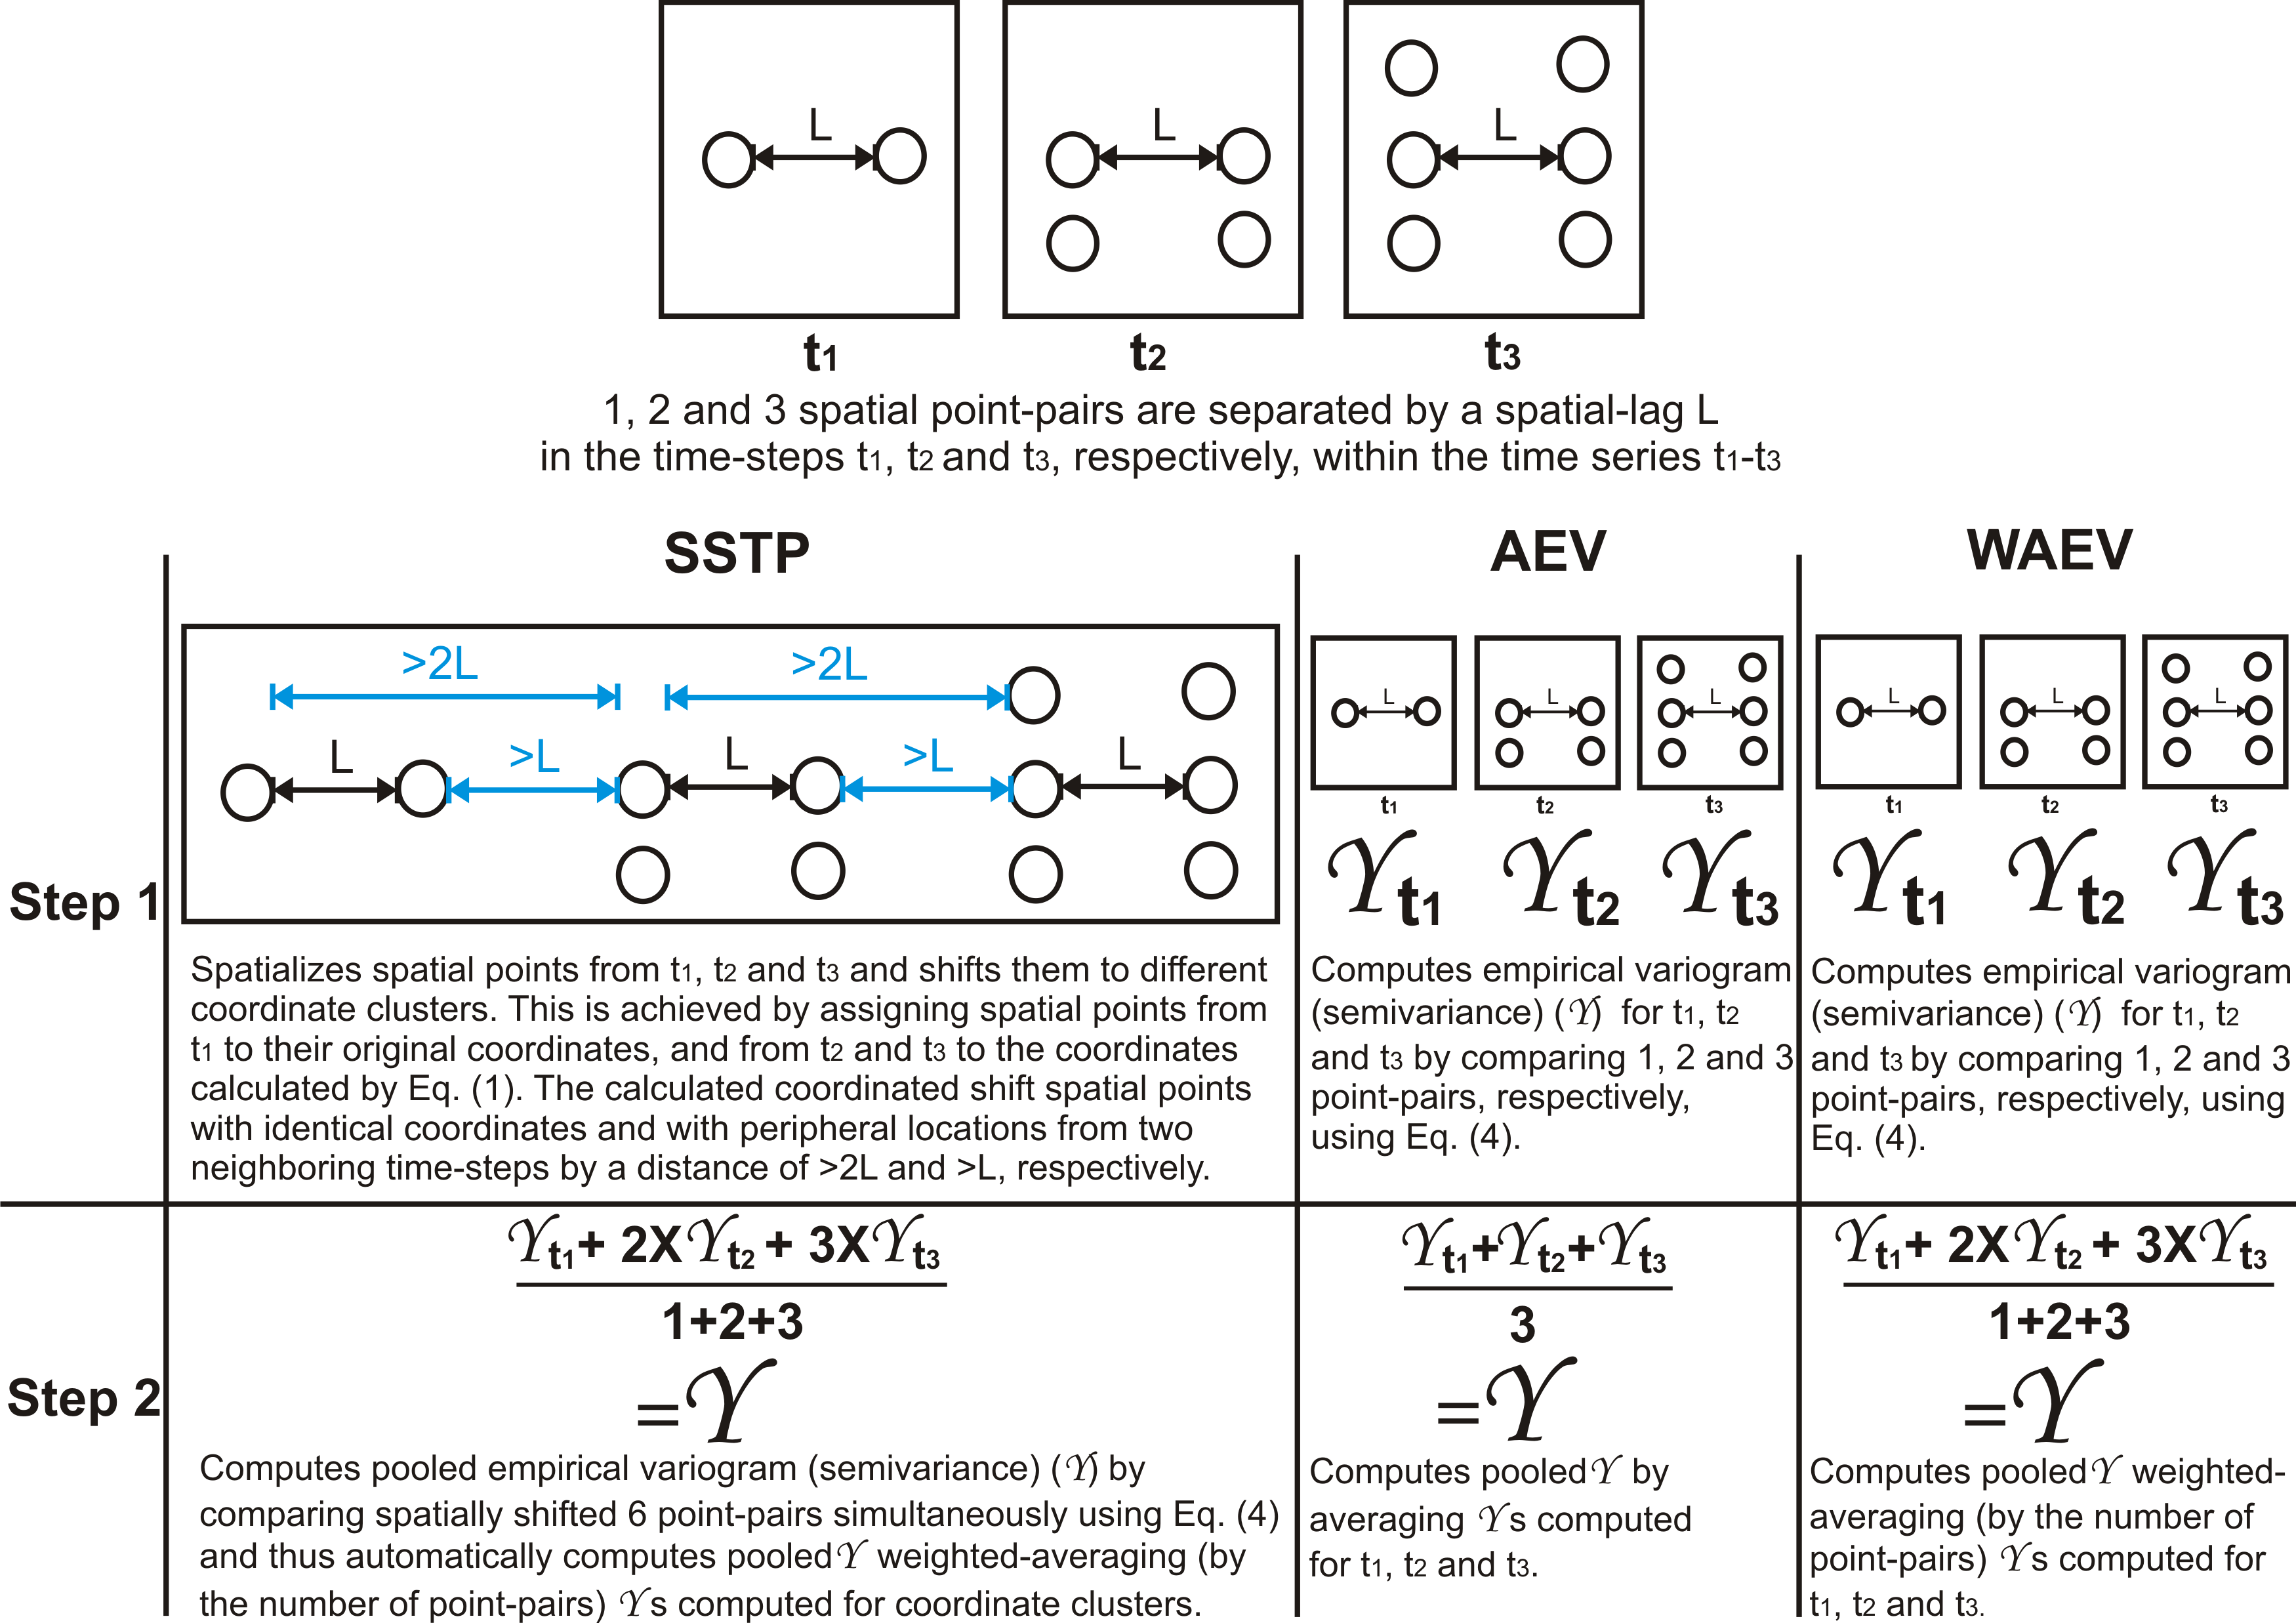
\includegraphics[width=\textwidth]{Figures/Fig_3_1.png}
  \caption{Work-flows and methodological differences between spatially shifting temporal points (SSTP), averaging empirical variograms (AEV) and weighted averaging empirical variograms (WAEV) methods for computing pooled within-time series (PTS) empirical variograms. PTS empirical variogram computation by AEV followed method c described in Gräler et al. (2011) and the method described in Pebesma and Gräler (2014).}
  \label{Fig_3_1}
\end{figure}

\begin{equation}
\begin{split}
s_{(t_1+1)+4n} = x_{(t_1+1)+4n}+(n+1)d, y_{(t_1+1)+4n} \\
s_{(t_1+1)+4n+1} = x_{(t_1+1)+4n+1}-(n+1)d, y_{(t_1+1)+4n+1} \\
s_{(t_1+1)+4n+2} = x_{(t_1+1)+4n+2}, y_{(t_1+1)+4n+2}+(n+1)d \\
s_{(t_1+1)+4n+3} = x_{(t_1+1)+4n+3}, y_{(t_1+1)+4n+3}-(n+1)d
\end{split}
\end{equation}

For example, for the years $t = {1949, 1950, 1951, 1952}$ within the pooled series of 1948-1975, $n = 0$ because   and $(1948+1)+4*0\leqt<(1948+1)+4(0+1)$ hence,

\begin{equation}
\begin{split}
s_{1949} = x_{1949}+d, y_{1949} \\
s_{1950} = x_{1950}-d, y_{1950} \\
s_{1951} = x_{1951}, y_{1951}+d \\
s_{1952} = x_{1952}, y_{1952}-d
\end{split}
\end{equation}

$d$ in Eqs. (3.1) and (3.2) is a shift distance that is bigger than two-fold the largest spatial-lag available within the pooled time series, i.e. $d>2*max||s_{i,t}-s_{j,t}||$, and shifts the data point sets of different years from each other. This shift distance was chosen because it prevents the influence of data point sets from different years on each other while estimating PTS variograms, i.e. the peripheral data points of the sets from neighboring years are separated by a distance outside of the range of the largest spatial-lag available within the pooled time series (Figure 3.1). Thus the shift distance represents a spatially rescaled temporal distancebetween data point sets from two consecutive years that preserves the spatiotemporal properties of PRCPTOT. Note that this shift distance is different from the spatially rescaled temporal distance computed for spatiotemporal variogram estimation in Gräler et al. (2011), where temporal variability was examined on a scale analogous to spatial variability. We selected the shift distance as in Eq. (3.3), but the users can choose any distance that is $>2*max||s_{i,t}-s_{j,t}||$.

\begin{equation}
d=2*max||s_{i,t}-s_{j,t}||+max||s_{i,t}-s_{j,t}||/100
\end{equation}

Spatial shifting of the temporal data points was performed using the R package “spacetime” (Pebesma, 2012). This allows for treating all temporal data points within a pooled time series as spatial points on the same space and thus for simultaneously binning and comparing point pairs from all time steps (spatial clusters) for a temporally constant spatial-lag. Moreover, point pairs from the cluster with the highest data density, where data points are separated by the smallest spatial-lag can be included in the temporally constant empirical variogram computation and thus uncertainties of short distance variability modeling for the clusters, where point pairs are only separable by larger spatial lags, are reduced.

Finally, the semivariances were computed by simulatenous comparison of all possible point pairs from the spatially shifted points using the commonly applied Methods of Moments (MoM) (Webster and Oliver, 2007). For the point pair $s_i$ and $s_j$ (both treated as spatial points on the same space), the semivariance $\gamma||s_i-s_j||$ (temporally constant) is a function of the spatial lag $||s_i-s_j||$ that is not affected by actual location of data points was computed by Eq. (3.4).

\begin{equation}
\gamma||s_i-s_j||=\frac{1}{2M||s_i-s_j||}\sum_{i,j}(Z(s_i)-Z(s_j))^2
\end{equation}

$M||s_i-s_j||$ is the number of point pairs that can be separated by the spatial lag $||s_i-s_j||$. Thus, SSTP uses a spatial variogram  computation method on the spatialized temporal points from a pooled time series and thus computes a temporally constant semivariance for each spatial-lag. In Eq. (3.4), the upper and lower boundaries of $||s_i-s_j||$ were set to the smallest and largest spatial-lags available within the pooled time series, respectively, according to Eq. (3.5).

\begin{equation}
\begin{split}
||s_i-s_j||_{smallest}=min||s_{i,t}-s_{j,t}||\\
||s_i-s_j||_{largest}=max||s_{i,t}-s{j,t}||
\end{split}
\end{equation}

These (Eq. 5) were done to reduce the uncertainty of modeling short distant spatial variability for the time steps with large spatial-lags, i.e. by modeling variability for the minimum spatial-lag within the time series (described above) and to avoid inclusion of temporal variability as pseudo spatial variability in semivariance computation, i.e. points that are temporally apart are not paired for comparison. Computation of semivariances was performed using “gstat” (Pebesma, 2004) package of R (R Core Team, 2015).

\subsubsection{Averaging empirical variograms (AEV)}
\label{Averaging empirical variograms (AEV)}

We also computed pooled semivariances using the AEV method (Figure 3.1). AEV corresponds to the method c described in Gräler et al. (2011) and the pooled variogram estimation method described in Pebesma and Gräler (2014). Semivariances for a temporally constant spatial-lag were computed for the individual time steps, where point pairs were separable by that spatial-lag. These semivariances from individual time steps were averaged to obtain the PTS semivariance.

\subsubsection{Weighted averaging empirical variograms (WAEV)}
\label{Weighted averaging empirical variograms (WAEV)}

We manually modified the AEV method for a more robust computation of pooled semivariances by taking the varying number of compared point pairs in individual time steps into account, i.e. WAEV (Figure 3.1). Semivariances for a spatial lag were computed in individual time steps as for AEV that were then averaged using a weighted approcah. The weights were provided according to the number of point pairs used for comparison in indiviual time steps.

\subsection{Test for anisotropy}
\label{Test for anisotropy}

After computation of semivariances using the above three methods, we checked for anisotropy in the spatial variability of the hydrological variable within the pooled time series. In case that anisotropy was detected, we computed the ratio between the major $(A)$ and minor $(B)$ axes of the anisotropy ellipse and the angle of the anisotropy $(\phi)$. Anisotropy parameters were computed using “intamap” package (Pebesma et al. 2011) and were converted according to the requirements of “gstat” (Pebesma, 2004) package in R (R Core team, 2015).

\subsection{Estimation and precision of PTS variograms}
\label{Estimation and precision of PTS variograms}

We estimated PTS variograms, i.e. fitted variogram models to the PTS empirical variograms for each pooled time series. Thereafter, the precision of estimated PTS variograms was evaluated by: (i) variogram model-fit to the empirical variograms and (ii) cross-validation of an appropriate kriging interpolation of the hydrological variable using the best-fit model (Webster and Oliver, 1992, 2007).

\subsubsection{Variogram model-fit}
\label{Variogram model-fit}

The available variogram models were fitted to the computed semivariances by a weighted least square approach providing $\frac{M(s_i,s_j)}{||s_i-s_j||^2}$ as weights (see Pebesma (2004) for details). However, variogram models can also be fitted by the maximum likelihood approach as described in Marchant and Lark (2007) or by providing different weights than ours if using the weighted least square approach (Pebesma, 2004). Details on the available variogram models and their formularization, and fitting in the gstat package (Pebesma, 2004) of R (R Core Team, 2015) can be found in Cressie (1983) and Pebesma (2001), respectively. The parameters of the fitted models, i.e. nugget and sill variances, and range (a) were extracted. In case that anisotropy was detected, the isotropic range parameter a was adjusted using the anisotropy parameter where geometric anisotropy was made isotropic according to Eq (3.6) through a linear transformation of coordinates with reference to the anisotropy ellipse described above (Oliver, 2010).

\begin{equation}
a=\sqrt{A^2cos^2\phi+B^2sin^2\phi}
\end{equation}

We computed the weighted mean of squared error (WMSE) as a model-fit statistic (Pebesma, 2004). The WMSEs of the previously fitted variogram models were compared and the best-fit model form with the lowest WMSE was identified for each pooled series.

\subsubsection{Kriging interpolation and performance statistics}
\label{Kriging interpolation and performance statistics}

The best-fit model form was used in a leave-one-out cross-validation of the spatial interpolation of the hydrological variable in each time step of each pooled series using an appropriate geostatistical interpolation technique, i.e. kriging. The kriging interpolation method was chosen because it gives unbiased evaluation of how well the variogram model fits the data (Oliver, 2010). The appropriate kriging technique was chosen based on the existance of spatial stationarity (described in 3.2.1) and covariates. The covariates were identified by checking spatial correlation between the hydrological variable and available other spatially dependent variables. Spatially dependent variables showing statistically significant correlation with the hydrological variable were chosen as covariates. In case that no convariate was identified and the hydrological variable showed spatial stationarity, ordinary kriging (OK) technique was used. Whereas in the presence of a trend in the regionalized variable mean, i.e. spatial non-stationarity, we used universal kriging (UK) technique. Kriging with external drift (KED) was used if covariates were available. Kriging interpolation was performed using the R (R Core Team, 2015) package “gstat” (Pebesma, 2004). For details on the kriging interpolation techniques and implementation in “gstat”, see Cressie (1983) and Pebesma (2004).

Finally, the root mean squared error (RMSE) and Nash-Sutcliffe efficiency (NSE) (Parajka et al., 2015) were computed as kriging interpolation performance statistics for each model form by comparing the observed and kriging interpolated hydrological variable values through a leave-one-out cross-validation (Pebesma, 2004). Note that we avoided the recalibration of the model form based on RMSE and NSE computed through the cross-validation because cross-validation statistics can be related to many factors other than the variogram model, such as the implementation of parameters related to the search neighborhood and used interpolation algorithm (Goovaerts, 2000).

The precision of the PTS variograms estimated by SSTP, AEV and WAEV for a pooled series were compared using correspondingWMSEs, RMSEs and NSEs.The method that estimated PTS variograms with the lowest WMSE and RMSE, and the highest NSE was chosen as the most precise variogram estimation method. To identify the effect of the consistency of spatial structure within a pooled time series on PTS variogram estimation, we also pooled the data points from a series showing inconsistent spatial structure, checked for temporal and spatial stationarity, and number and density of pooled data points and used for PTS variogram estimation. The MSEs and RMSEs, and NSEs of these PTS variograms were compared with the PTS variograms estimated for time series with consistent spatial structure.

We provide a commented R-script as a supplementary material (R\textunderscore script.R in the supplemetary material) detailing the SSTP and enabling comparison with AEV and WAEV methods for PTS variogram estimation. The sample data (Sample\textunderscore data.Rdata) for reproducibility is also provided in the supplementary material. For further modification and development of SSTP, the R-script and sample data are available from an online repository, i.e. \href{https://github.com/AvitBhowmik/SSTP}{https://github.com/AvitBhowmik/SSTP}.


\section{Study area and data}
\label{Study area and data}

The above three methods were applied to the PTS variogram estimation for “annual total precipitation in hydrological wet days (PRCPTOT)” in Bangladesh (Peterson et al., 2001) (Figure 3.2) and their precision statistics were compared. The hydrological wet days in Bangladesh refer to the monsoon season, i.e. June to September in each year, when 80 \% of the annual precipitation occurs (Bhowmik, 2012; DMICCDMP, 2012). We used the daily precipitation data from 1948-2007 series that were collected from Bangladesh Meteorological Department (DMICCDMP, 2012). Currently, 32 rain-gauges (density 2.2 rain-gauges per 10000 sq. km.) report daily precipitation in Bangladesh, classifying the country as data scarce (Webster and Oliver, 2007) (Figure 3.3). Moreover, the numbers of data points and data density exhibit an increasing coverage from 8 points in 1948 to 32 points in 2007, and from 0.5 points per 10000 sq. km in 1948 to 2.2 points per 10000 sq. km in 2007, respectively (Figure 3.3, details can be extracted from Figure B.1 and Table B.1 in appendix B). This indicates an increase in the precision of variogram estimation from 1948 to 2007. However, spatial variograms estimated for all individual years are likely imprecise as all are estimated with $<$ 50 data points and $<$ 3 points per 10000 sq. km. (Webster and Oliver, 2007) (Figure 3.3).

The precipitation data were quality controlled and validated using the “RClimdex” routine (Peterson et al., 2001). Then, PRCPTOT was computed for each of the time steps (year) and data points (rain-gauge) where precipitation data were available following the method described in Bhowmik (2012) and Peterson et al. (2001). To identify covariates, we checked for the spatial correlation between PRCPTOT and the elevation of data points.

\begin{figure}[t]
  \centering
  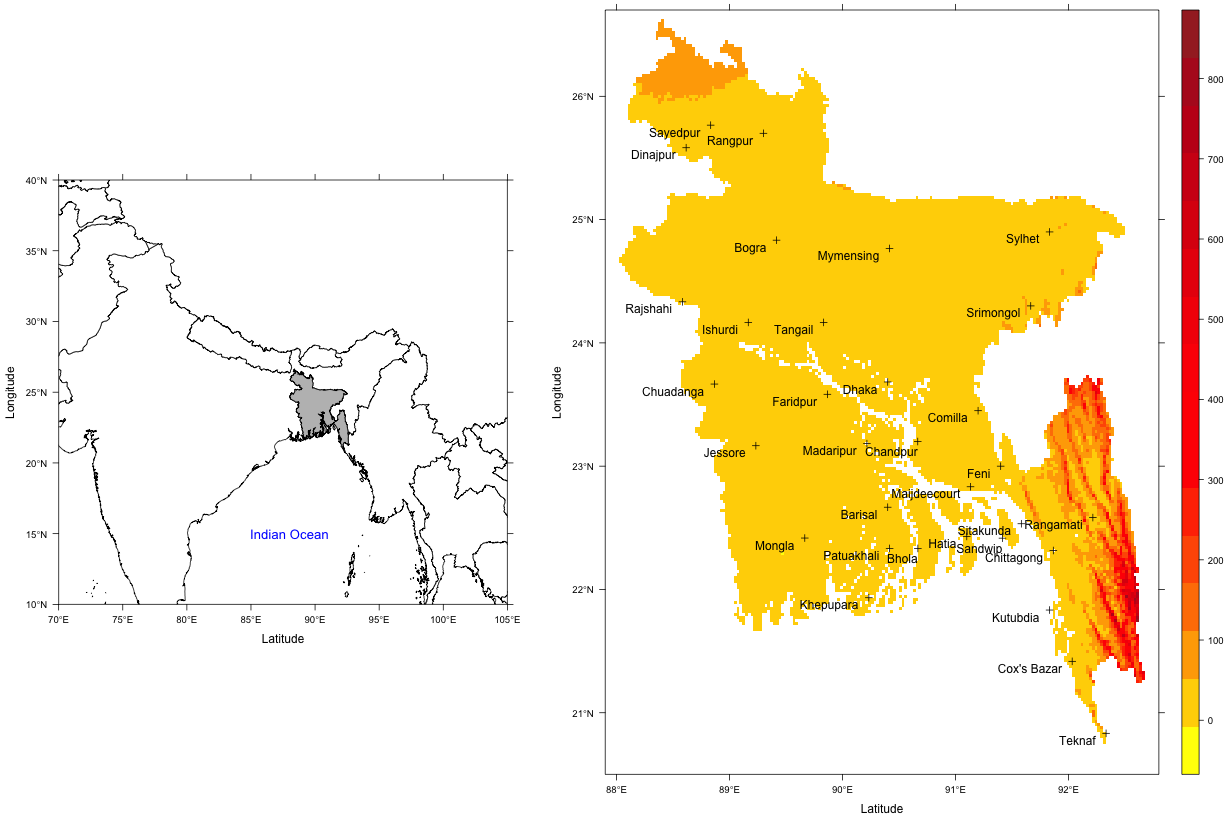
\includegraphics[width=\textwidth]{Figures/Fig_3_2.png}
  \caption{Geographic location of Bangladesh (left) in Southeast Asia within the coastal belt of Indian Ocean and the spatial distribution of currently active 32 rain-gauges (right) with altitudes (m above mean sea level) in the background. The coordinate reference system is WGS 1984.}
  \label{Fig_3_2}
\end{figure}

\begin{figure}[t]
  \centering
  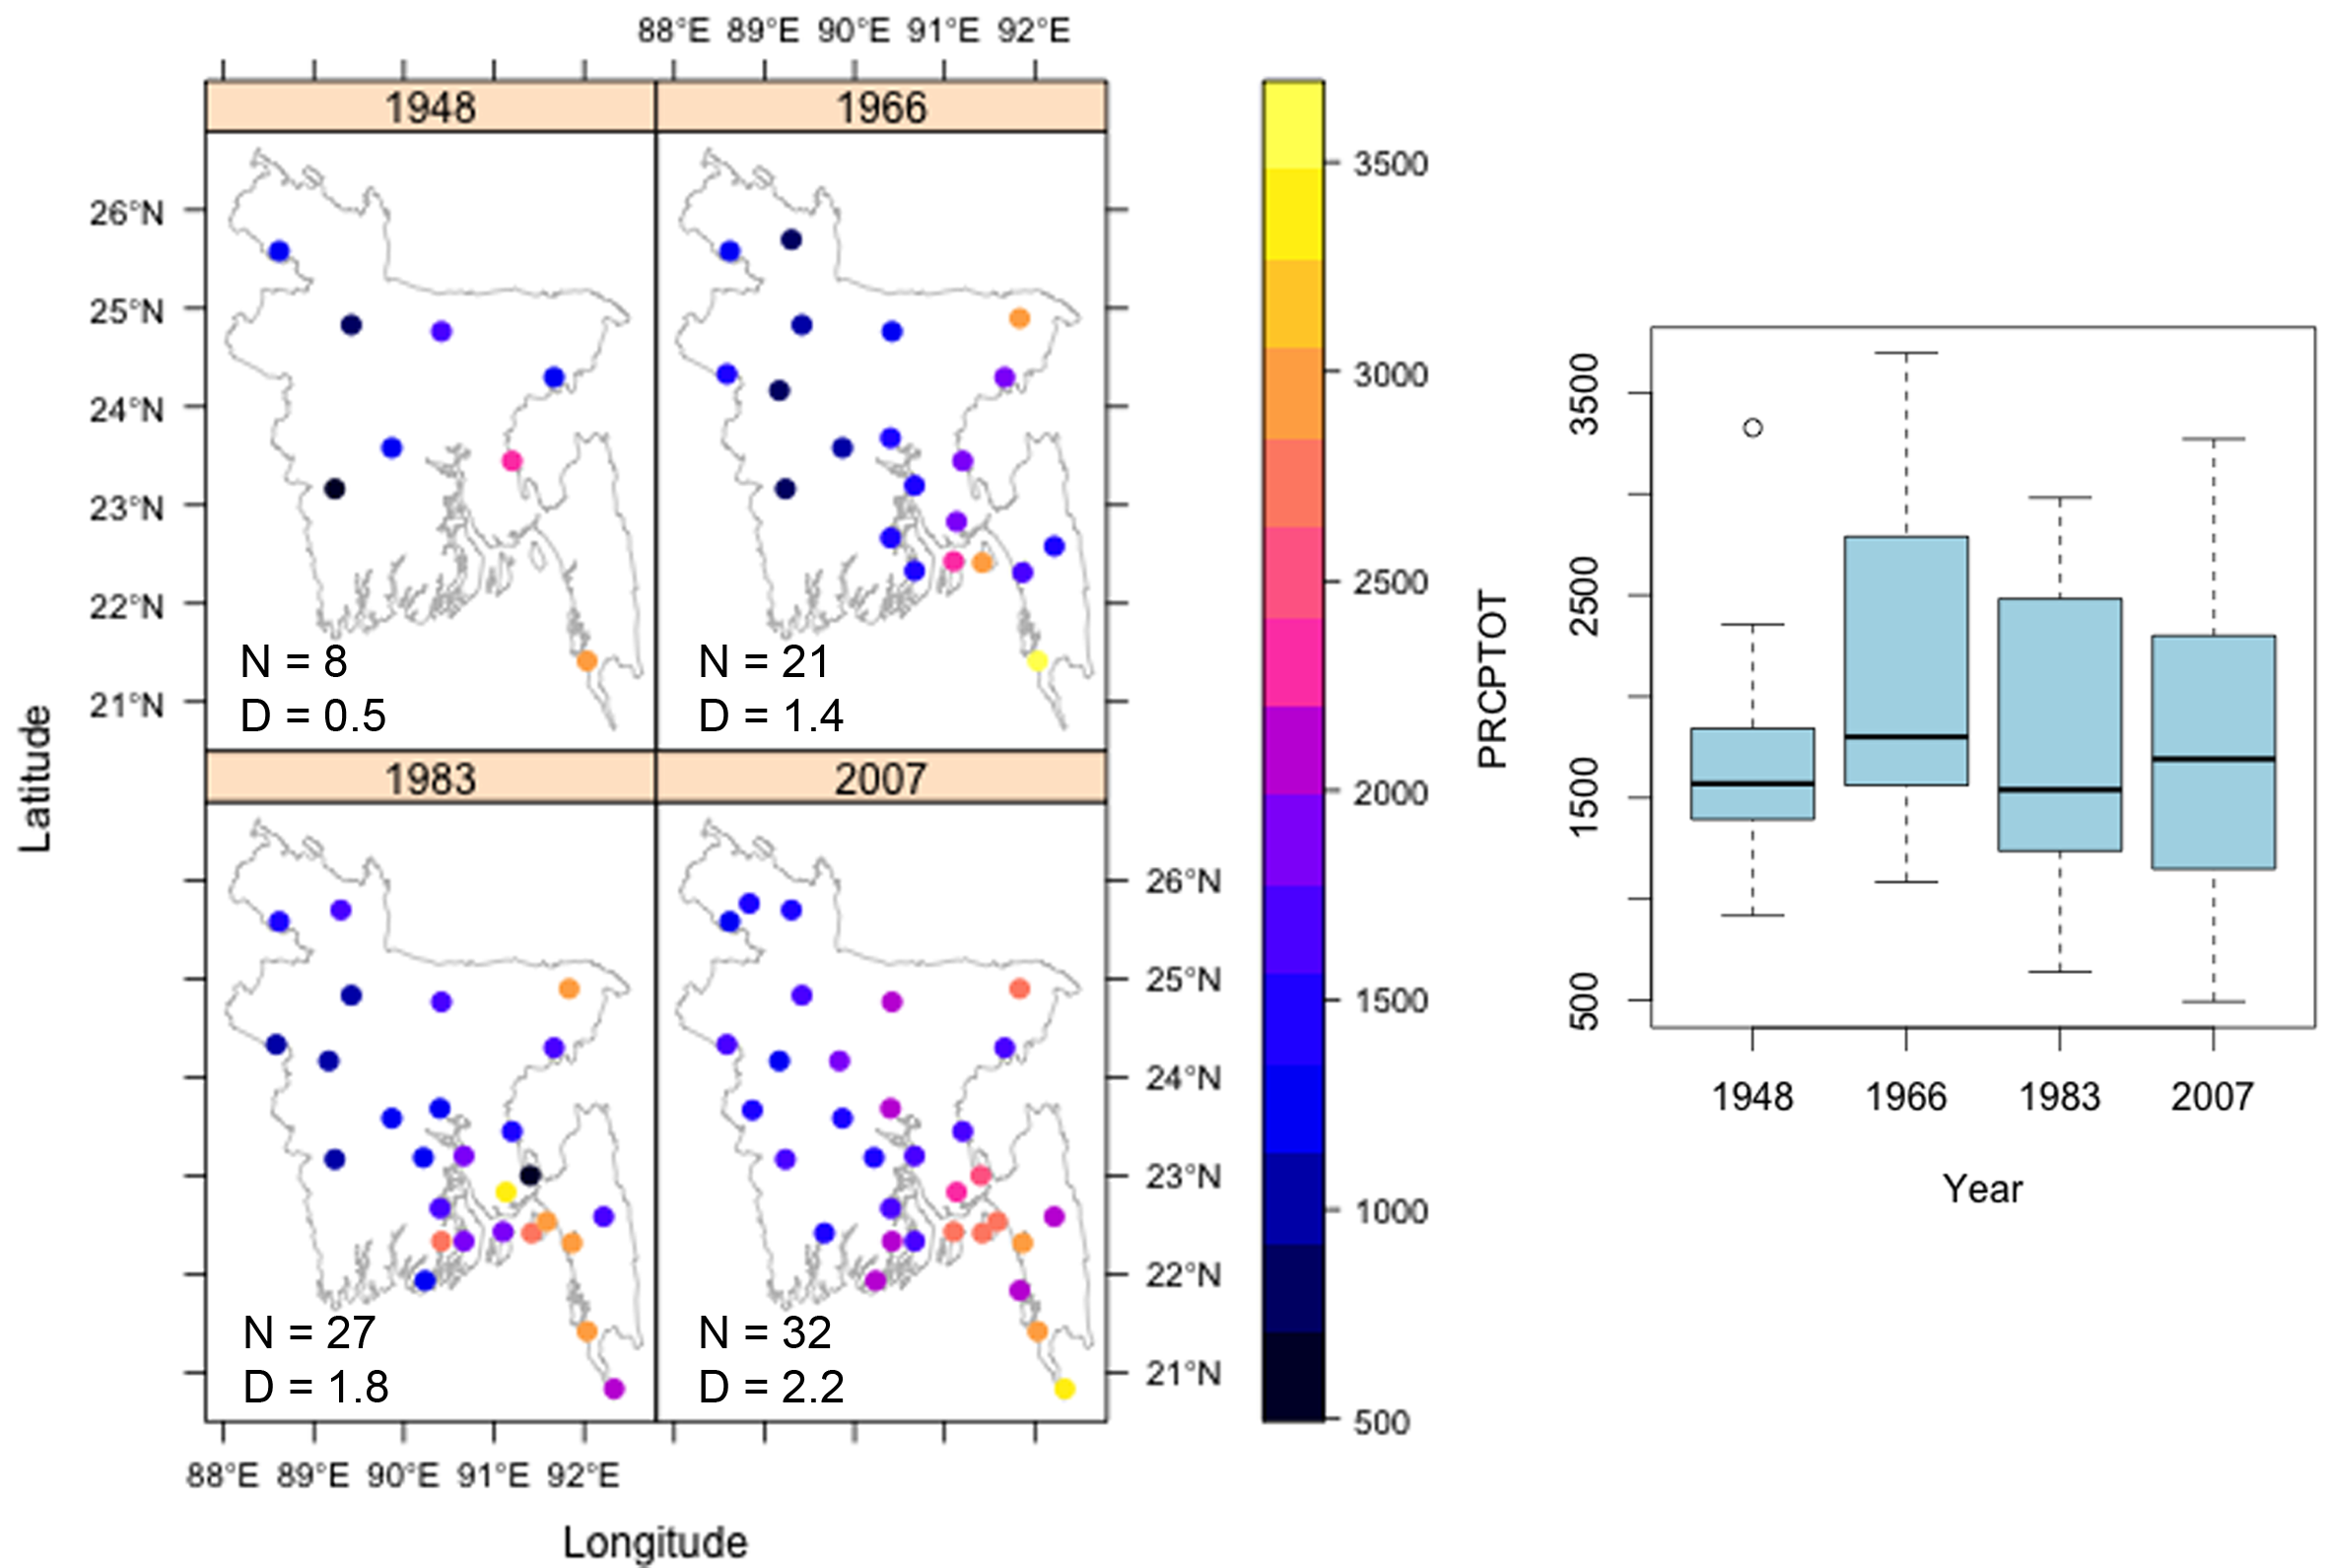
\includegraphics[width=\textwidth]{Figures/Fig_3_3.png}
  \caption{Temporally varying spatial locations, numbers (N) and density (D, in points per sq. km) of data points (left), and magnitude (in mm) and distribution of the computed annual total precipitation in hydrological wet days (PRCPTOT) (right) in Bangladesh during 1948-2007 series for four representative years, i.e. 1948, 1966, 1983 and 2007. Details on the spatial locations, N, D, magnitude and distribution of PRCPTOT in each year during 1948-2007 are available from Figure B.1 and Table B.1 in the appendix B.}
  \label{Fig_3_3}
\end{figure}

\section{Results}
\label{Results}

\subsection{Spatial structure and stationarity}
\label{Spatial structure and stationarity}

Statistically significant change points were detected in 1976 and 1993, and in 1976 for the spatial correlation coefficients of PRCOTOT along the longitudinal and latitudinal gradients, respectively, within the 1948-2007 series (Figure 3.4). These change points indicated changes in spatial structure from 1976 and 1993. Consequently, spatial structure within the entire 1948-2007 series was inconsistent whereas the (sub)time series 1948-1975, 1976-1992 and 1993-2007 showed consistent spatial structure.

\begin{figure}[t]
  \centering
  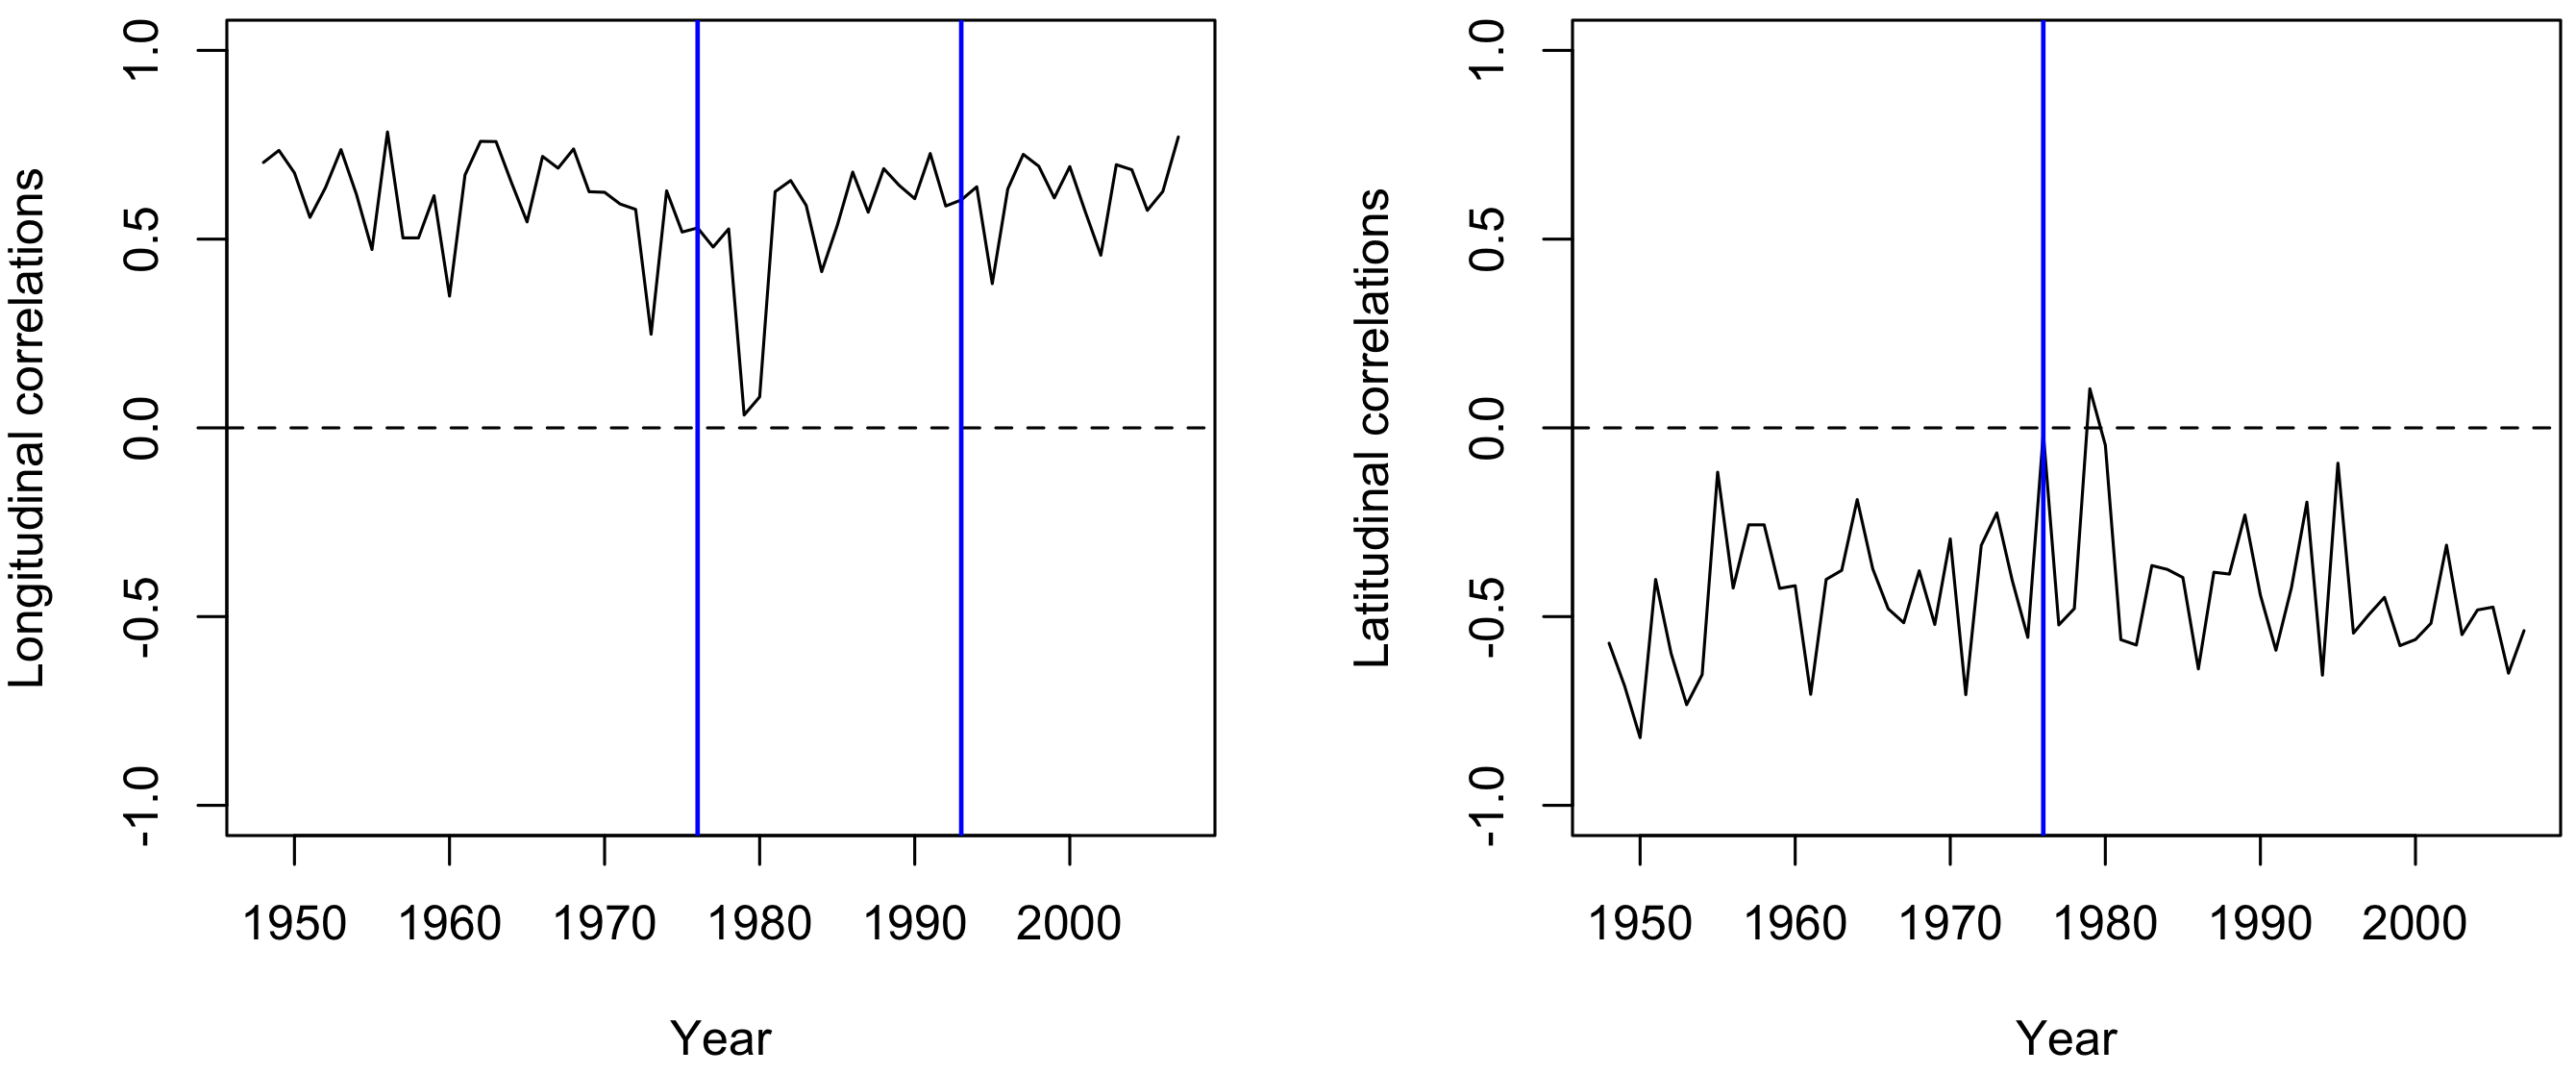
\includegraphics[width=\textwidth]{Figures/Fig_3_4.png}
  \caption{Statistically significant change points in the spatial correlations of annual total precipitation in hydrological wet days (PRCPTOT) along the longitudinal (left) and latitudinal (right) gradients within the 1948-2007 series.}
  \label{Fig_3_4}
\end{figure}

The Dickey-Fuller statistics obtained for the 1948-1972, 1976-1992, 1993-2007 and 1948-2007 series were -4.5, -3.4, -5.0 and -4.0 respectively, and they were statistically significant at p $<$ 0.01. Therefore, for each of these series null hypothesis was rejected and thus PRCPTOT showed temporal stationarity. Moreover, the number of total data points within the 1948-1975, 1976-1992, 1993-2007 and 1948-2007 series met the threshold for reliable variogram estimation (Table 3.1).

\begin{table}[h]
\label{Table 3.1}
\caption{Number of data points, smallest and largest spatial-lags, and summary statistics, i.e. minimum (Min.), mean, maximum (Max.) and coefficient of variation (CV) of annual total precipitation in hydrological wet days (PRCPTOT) within the pooled time series.}
\begin{threeparttable}
\centering
\begin{tabular}{>{\centering\arraybackslash}m{2.2cm}>{\centering\arraybackslash}m{2.0cm}>{\centering\arraybackslash}m{1.5cm}>{\centering\arraybackslash}m{1.0cm}>{\centering\arraybackslash}m{1.0cm}>{\centering\arraybackslash}m{0.7cm}>{\centering\arraybackslash}m{0.7cm}>{\centering\arraybackslash}m{0.7cm}>{\centering\arraybackslash}m{0.7cm}}

\toprule
\textbf{Pooled time series} & \textbf{Number of pooled data points} & \textbf{Data density} & \multicolumn{2}{c}{\textbf{Spatial lag}} & \multicolumn{4}{c}{\textbf{PRCPTOT}}\\
 & & & \textbf{Smallest} & \textbf{Largest} & \textbf{Min.} & \textbf{Mean} & \textbf{Max.} & \textbf{CV}\\
 & & \textbf{(point/10000 $km^2$)} & \textbf{$(km)$} & \textbf{$(km)$} & \textbf{$(mm)$} & \textbf{$(mm)$} & \textbf{$(mm)$} & \textbf{(\%)}\\

\midrule

1948-1975 & 441 & 1.5 & 29.16 & 550 & 17 & 1659 & 4036 & 42\\
1976-1992 & 465 & 2.2 & 26.61 & 550 & 84 & 1759 & 4499 & 42\\
1993-2007 & 475 & 2.2 & 27.51 & 550 & 29 & 1789 & 4516 & 41\\
1948-2007* & 1381 & 2.2 & 26.61 & 550 & 17 & 1738 & 4516 & 41\\

\bottomrule

\end{tabular}
\begin{tablenotes}
\footnotesize
* Pooled time series with inconsistent spatial structure
\end{tablenotes}
\end{threeparttable}
\end{table}

Statistically significant positive and negative spatial trends were observed in PRCPTOT along the logitudinal (363.90 mm/0, p $<$ 0.001) and latitudinal (-246.73 mm/0, p $<$ 0.001) gradients. Therefore, regionaliged PRCPTOT depicted trend in the mean and hence, exhibited spatial non-stationarity. This is also supported by Figure 3.3, where a gradual increase in PRCPTOT was observed from the Northwest to Southeast of Bangladesh. 

\subsection{Pooled within-time series (PTS) empirical variograms}
\label{Pooled within-time series (PTS) empirical variograms}

\subsubsection{Spatial shifts}
\label{Spatial shifts}

The distance $d$ used for spatial shifting by spatially shifting temporal points (SSTP) method in each of the pooled series was 1111 km ($~10^0$, decimal degree as a geographical measure of longitude or latitude with WGS 1984 datum) because the largest spatial-lag available within these series was approximately 550 km ($~5^0$) (Figure 3.5; Table 3.1). Thus the shifted peripheral data points sets from neighboring years showed a distance $>$ 550 km, i.e. $\geq$ (1111-550) km (Figure 3.5), and therefore the spatiotemporal properties of PRCPTOT were preserved, i.e. the data points from a year did not influence data points from other years and temporal autocorrelation was coherent with the spatial autocorrelation of the spatialized point clusters (Figure 3.5). Consequently, the shift distance represents a spatially rescaled temporal distance (1 year) between data point sets from two consecutive years that preserves the spatiotemporal properties of PRCPTOT.

\subsubsection{Empirical variograms}
\label{Empirical variograms}

SSTP computed a single temporally constant semivariance of PRCPTOT for each spatial-lag by simultaneously comparing point pairs from all years that are separable by that spatial-lag (Figure 3.5; 3.6). For example, for the pooled series of 1948-1975, point pairs with PRCPTOT observations that were separated by 100 km in each of the 25 clusters could be binned and compared simultaneously for a single empirical variogram computation (Figure 3.5; 3.6). Consequently, the number of point pairs for comparison could be increased to 441 as they were pooled from 25 clusters (years) (Table 3.1). Departing from SSTP, the averaging empirical variograms (AEV) and weighted AEV (WAEV) methods computed yearly semivariances for each spatial lag, i.e. computed separate semivariance for each SSTP coordinate cluster, and averaged them arithmatically and weighting by the number of comapred point pairs in each cluster, respectively. Consequently, the SSTP and WAEV computed semivariances were much less noisy than the semivariances computed by AEV, especially for large spatial-lags (Figure 3.6).

\subsubsection{Data density and short distance variabiity}
\label{Data density and short distance variabiity}

Data density for 1948-1975 series could be increased to 1.5, and for 1976-1992, 1993-2007 and 1948-2007 to 2.2 points per 10,000 sq. km for PTS variogram estimation (Table 3.1). Consequently, the smallest spatial-lags available within the three pooled series allowed for modeling spatial variability of PRCPTOT at $\leq$ 29 km (Table 3.1). This, particularly, decreased uncertainty for short distant spatial variability modelling for the time steps where the smallest spatial-lags were substantially higher, i.e. $\geq$ 60 km for 1948-1965.

\subsubsection{Anisotropy}
\label{Anisotropy}

Anisotropy was detected in the spatial variability of PRCPTOT for all pooled series in the northwest-southeast direction ($90^0>\phi>0^0$ from normal north to anticlockwise, for details see Pebesma (2004)) indicating a strong variability of PRCPTOT in that direction (Figure 3.6). This is also coherent with the direction of spatial trend in PRCPTOT (Figure 3.3) and the strong spatial variation of PRCPTOT within the pooled time series, i.e. CV $\geq$ 41 \% (Table 3.1). Moreover, 1948-1975 series depicted weak anisotropy ($A:B=0.8$), i.e. relatively weak variability whereas 1976-1992 and 1993-2007 series depicted strong anisotropy ($A:B=0.4$), i.e. relatively strong variability (Figrue 3).

\subsection{Precision of variogram estimation}
\label{Precision of variogram estimation}

\subsubsection{Variogram model-fit}
\label{Variogram model-fit}

The “Power” (Pow) model showed the best fit, i.e. the lowest weighted mean of squared error (WMSE) for all methods in all pooled series (Figure 3.6). This indicates a monotonic increase in empirical variograms with an increase in the spatial-lags without reaching a threshold and hence spatial non-stationarity, which is supported by the presence of a trend in the mean of PRCPTOT (Figure 3.3).

The PTS variograms estimated by SSTP showed better model-fit (lower WMSE, i.e. $4.54 X 10^7$ on average) than the AEV (average MSE: $7.52 X 10^8$), WAEV showed identical better model-fit than AEVto SSTP (Table 3.2). The PTS variograms estimated for the time series with inconsistent spatial structure, i.e. 1948-2007, by all methods showed higher WMSE than the variograms estimated for the time series with consistent spatial structure (Table 3.2). For the time series with consistent spatial structure, WMSEs for PTS variogram estimation decreased with the increasing number of pooled data points (Table 3.2).

\begin{table}[h]
\label{Table 3.2}
\caption{Precision statistics of the pooled within-time series (PTS) variograms estimated by spatially shifting temporal points (SSTP), averaging empirical variograms (AEV) and weighted averaging empirical variograms (WAEV) methods. The weighted mean of squared errors (WMSE) as the variogram model-fit statistic, and root means squared error (RMSE) and Nash-Sutcliffe efficiency (NSE) as the universal kriging interpolation performance statistics are presented.}
\begin{threeparttable}
\centering
\begin{tabular}{>{\centering\arraybackslash}m{1.7cm}>{\centering\arraybackslash}m{1.2cm}>{\centering\arraybackslash}m{1.2cm}>{\centering\arraybackslash}m{1.2cm}>{\centering\arraybackslash}m{0.8cm}>{\centering\arraybackslash}m{0.8cm}>{\centering\arraybackslash}m{0.8cm}>{\centering\arraybackslash}m{0.7cm}>{\centering\arraybackslash}m{0.6cm}>{\centering\arraybackslash}m{0.7cm}}

\toprule
\textbf{Pooled time series} & \multicolumn{3}{c}{\textbf{WMSE}} & \multicolumn{3}{c}{\textbf{RMSE}} & \multicolumn{3}{c}{\textbf{NSE}}\\
 & \textbf{SSTP} & \textbf{AEV} & \textbf{WAEV} & \textbf{SSTP} & \textbf{AEV} & \textbf{WAEV} & \textbf{SSTP} & \textbf{AEV} & \textbf{WAEV}\\

\midrule

1948-1975 & $2.55 X 10^7$ & $6.6.3 X 10^8$ & $3.21 X 10^7$ & $622.63$ & $655.41$ & $630.58$ & $0.28$ & $0.19$ & $0.25$\\
1976-1992 & $2.47 X 10^7$ & $4.49 X 10^8$ & $3.09 X 10^7$ & $597.98$ & $653.96$ & $624.54$ & $0.30$ & $0.21$ & $0.27$\\
1993-2007 & $2.43 X 10^7$ & $3.3.4 X 10 ^8$ & $2.96 X 10^7$ & $461.50$ & $493.95$ & $485.05$ & $0.53$ & $0.47$ & $0.49$\\
1948-2007* & $1.07 X 10^8$ & $1.56 X 10^9$ & $1.15 X 10^8$ & $655.85$ & $669.29$ & $665.12$ & $0.23$ & $0.10$ & $0.18$\\

\bottomrule

\end{tabular}
\begin{tablenotes}
\footnotesize
* Pooled time series with inconsistent spatial structure
\end{tablenotes}
\end{threeparttable}
\end{table}

\subsubsection{Kriging interpolation performance}
\label{Kriging interpolation performance}

The elevation of all data points was below 50 m (Figure 3.2) and did not significantly (p = 0.8) correlate with PRCPTOT in Bangladesh. Hence, because of the unavailability of spatial convariates and presence of spatial non-stationarity, universal kriging (UK) method proved to be the most appropriate for interpolating PRCPTOT in Bangladesh.

UK interpolation of PRCPTOT fitting the PTS variogram models estimated by SSTP entailed better performance in cross-validation than AEV, showing lower root mean squared error (RMSE) and higher Nash-Sutcliffe efficiency (NSE) (Parajka et al., 2015), and identical performance to WAEV (Table 3.2). Average RMSEs and NSEs obtained for UK interpolation by fitting the PTS variograms estimated by SSTP and WAEV, and AEV  were 584.49 and 0.34, and 618.15 and 0.24, respectively. Lower RMSEs and higher NSEs were also observed for UK interpolation of PRCPTOT fitting PTS variograms estimated by all methods for the time series with consistent spatial structure than with inconsistent spatial structure (Table 3.2). Decreasing RMSEs and increasing NSEs were also observed with the increasing number of pooled data points for the time series with consistent spatial structure.

Overall, SSTP estimated PTS variograms showed better fit to the empirical variograms and data and thus showed higher precision than AEV, while showed identical precision to WAEV (Table 3.2). Moreover, higher precision in variogram estimation was obtained for the time series with consistent spatial structure than the inconsistent spatial structure, while precision increased with the increasing number of pooled data points for consistent spatial structure (Table 3.2).

\begin{figure}[h!]
  \centering
  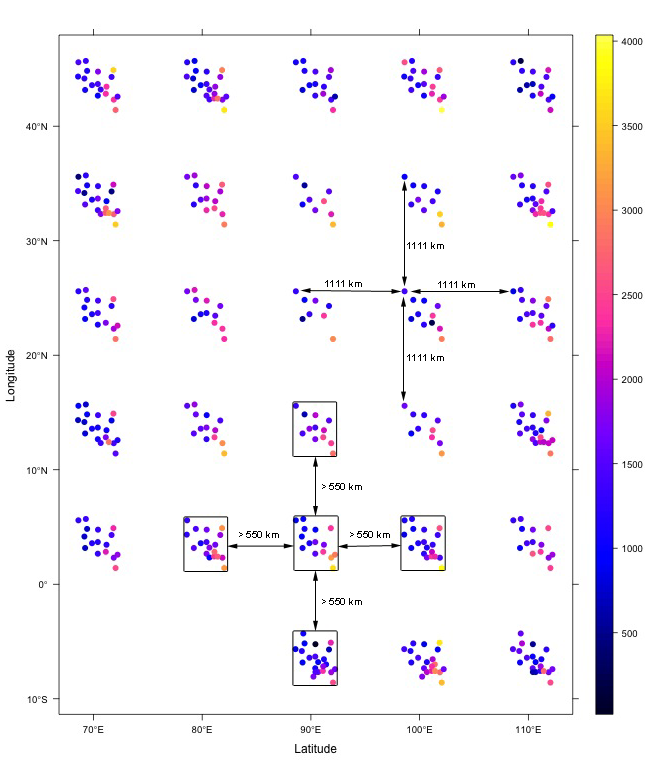
\includegraphics[width=\textwidth]{Figures/Fig_3_5.png}
  \caption{Spatially shifted (according to Eq. (1)) temporal data points for the pooled 1948-1975 series. Shift distance ($d$ = 1111 km) is calculated based on the largest-spatial-lag (550 km) available within the series (Eq. 3). The data point sets from neighboring years are shifted by 1111 km ($~10^0$), which ensures that the peripheral points of the sets are shifted by $>$ 550 km ($~5^0$). The rectangles and legend indicate peripheries (convex hull) of data points in a year and PRCPTOT in mm, respectively.}
  \label{Fig_3_5}
\end{figure}

\subsection{Discussion and future research challenges}
\label{Discussion and future research challenges}

In this paper, we developed and implemented spatially shifting temporal points (SSTP), an alternative method for estimating pooled within-time series (PTS) variograms in spatially data-scare regions. Contrasting with the available method of averaging empirical variograms (AEV)), which are computed for individual time steps, SSTP computed empirical variograms by simultaneously comparing all point pairs separable by a spatial-lag within a pooled time series (Figure 3.1; 3.6). Consequently, when compared to the PTS variograms estimated by AEV, SSTP variograms showed higher precision (Figure 3.6; Table 3.2). The numbers of available data points did not meet the threshold for satisfactorily precise variogram estimation in any of the individual time steps (year) within 1948-2007 series and data density were very low (Figure 3.3; B.1 and Table B.1). Hence, the available numbers of point pairs and smallest spatial-lags for comparisons were not sufficient for reliable semivariance computation (Webster and Oliver, 2007) (Figure 3.3). As a result, computed semivariances for the individual years were likely erratic that induced noisy and erratic semivariances when averaged by the AEV method (Figure 3.6). Thus model fitting to AEV semivariances showed a lower goodness-of-fit and universal kriging (UK) interpolation of PRCPTOT using the AEV and WAEV variogram models showed worse performance than the SSTP variograms (Figure 3.6; Table 3.2). By contrast, SSTP computed semivariances were reliable because of subtantially higher number of simultaneous comparisons and higher data density than by AEV (Table 3.1; 3.2) and thus entailed higher precision in PTS variogram estimation. These results are in line with Webster and Oliver (1992, 2007).

Semivariances computed for small spatial-lags by SSTP and AEV methods were similar whereas semivariances for large spatial-lags were largely different (Figure 3.6). Moreover, semivariances computed by AEV and WAEV showed much more noise at large spatial-lags than small spatial-lags. The number of erratic semivariances averaged by AEV for large spatial-lags were higher than for small spatial lags because point-pairs from more years were separable by large spatial-lags than by small spatial-lags due to data availability (Figure 3.3). For example, point pairs from only two years (1973 and 1975) were separable by the smallest spatial-lag for 1948-1975 series whereas point pairs from 20 years were separable by the largest spatial-lag (Table 3.1, B.1). In addition, the numbers and spatial locations of available data points are highly variable within the pooled series and spatial variability of PRCPTOT was high (Figure 3.3; Table 3.1). Hence, we argue that the averaged semivariances computed by AEV were representative of the small number of semivariances at small spatial-lags but unrepresentative of the large number of semivariances at large spatial-lags because of the variable number and spatial location of data points and high spatial variability of PRCPTOT. As a result, semivariances for large spatial-lags computed by SSTP and AEV could be similar if the numbers and spatial locations of data points were the same for all time steps and spatial variability of PRCPTOT was low (Gräler et al., 2011). However, for variable number and spatial locations of data points, the noise in the semivariances computed by AEV at large spatial-lags could be reduced by the manual modification to the robust WAEV method, i.e. by weighing the average of semivariances per spatial lag with the corresponding number of data points available per time step, and thus a better model-fit and UK interpolation performance could be achieved (Figure 3.6). Thus, SSTP automatically account for the varying numbers and locations of data points in a time series by weighting average semivariances and consequently entail identical variograms and precision to WAEV (Figure 3.1).

The PTS variograms estimated for the 1948-2007 series (inconsistent spatial structure) showed lower precision than the variograms estimated for the series with consistent spatial structure, although PRCPCTOT was stationary within 1948-2007 series, the number of data points (higher than for the series with consistent spatial structure) met the threshold for reliable variogram estimation and the highest data-density could be achieved (Webster and Oliver, 1992; 2007) (Table 3.1; 3.2). Moreover, higher precision was obtained for PTS variogram estimation with higher number of pooled data points among the series with consistent spatial structure and vice-versa (Table 3.1; 3.2). However, this may also be related to the inherent spatial structure within the time series, i.e. spatial variability of PRCPTOT may be estimated with higher precision for the data points with the spatial structure observed for 1993-2007 than for 1948-1975. Furthermore, the Hole model showed the best fit for the series with inconsistent spatial structure that did not represent the variability for individual time steps, i.e.Power variability was representative as depicted by the models for consistent spatial structure. These results suggest that the consistency of spatial structure, i.e. the strength of spatial variabilty within pooled time series is crucial for PTS variogram estimation (Kravchenko, 2003) and increasing the number of pooled data points and data density may increase the precision of PTS variogarm estimation when the spatial structure is consistent. Many studies pooled data points only by assuming the consistency of spatial structure within time series (Bhowmik, 2012; Gräler et al., 2011; Rogelis and Werner, 2012; Wagner et al., 2012). We recommend that time series should be checked for consistency of spatial structure before pooling.

The threshold for reliable variogram estimation, i.e. 400 data points (Webster and Oliver, 2007), could be achieved for each pooled series (Table 3.1). However, if data scarcity is more acute in a region and the required number of data points for reliable variogram estimation is unavailable, users

\clearpage

\begin{figure}[h!]
  \centering
  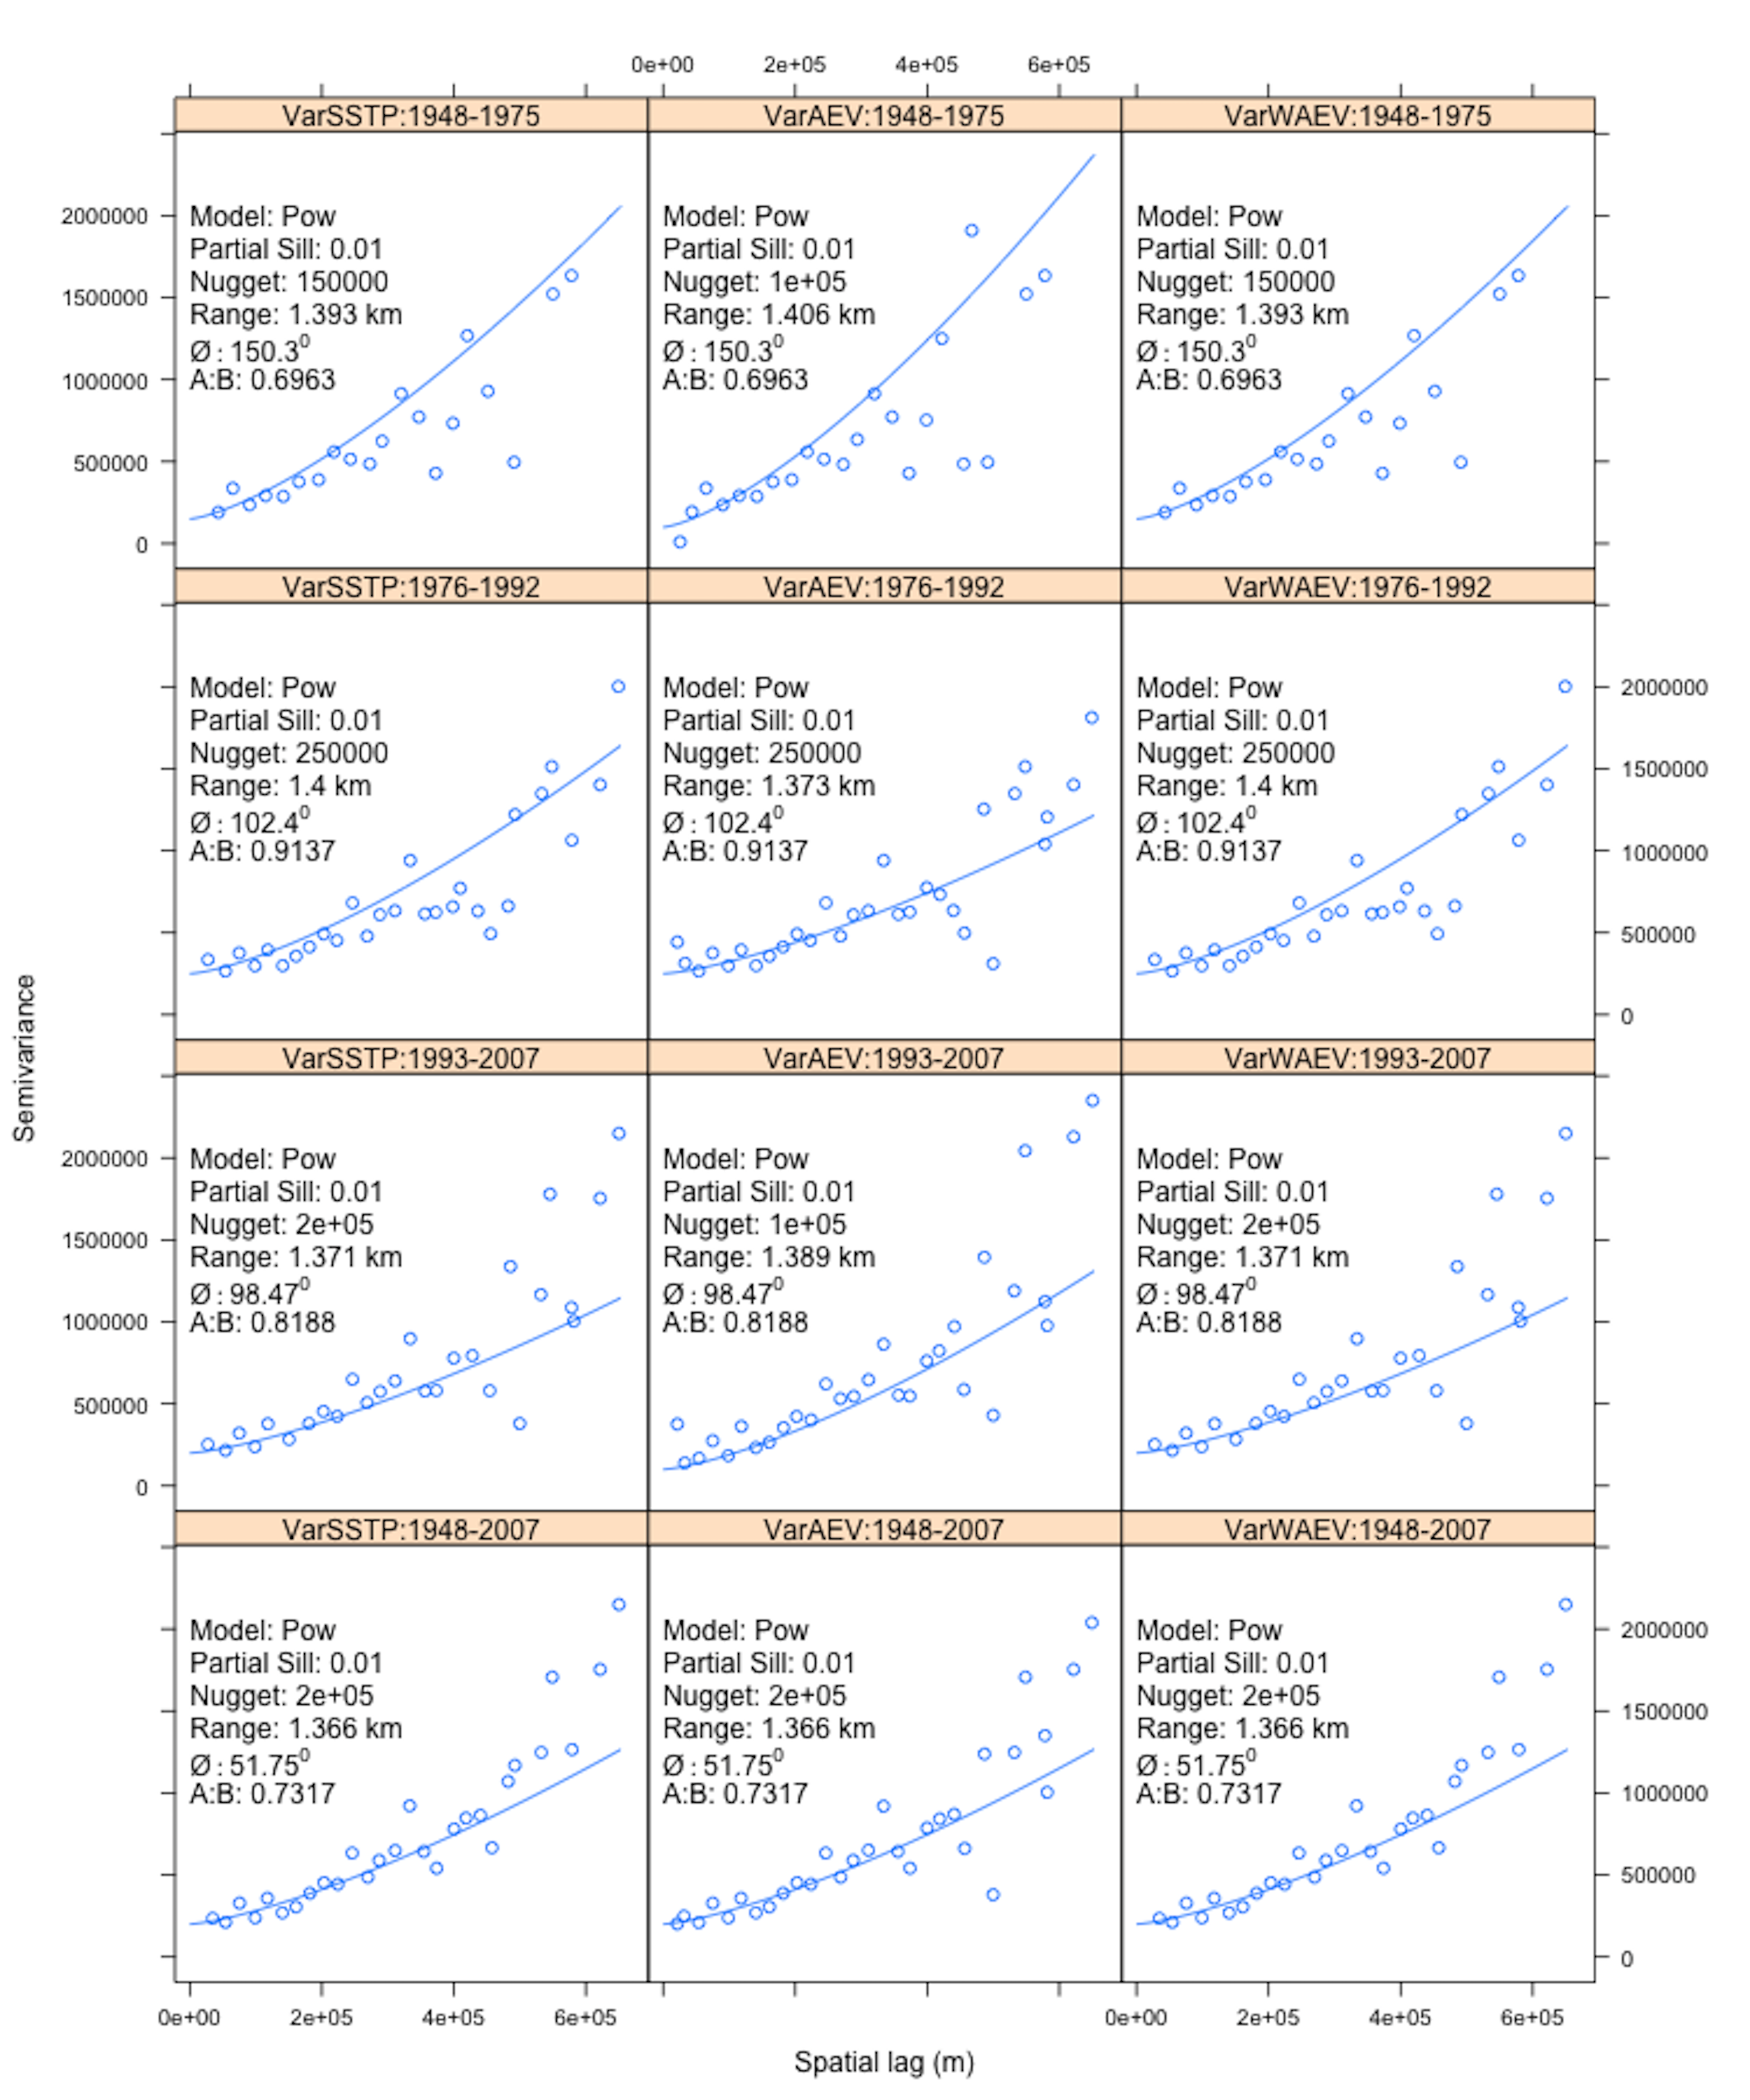
\includegraphics[width=\textwidth]{Figures/Fig_3_6.png}
  \caption{Estimated pooled within-time series (PTS) variograms (fitted best models to empirical variograms) by spatially shifting temporal points (SSTP), averaging empirical variograms (AEV) and weighted averaging empirical variograms (WAEV) methods. Figure captions depict variogram(Var) estimation method: pooled series. The “Power” (Pow) model was fitted according to $\gamma(||s_i-s_j||,\phi)=c_o+c_w||s_i-s_j||^a$, respectively, where $||s_i-s_j||$ represents the spatial lag between point pair $s_i$ and $s_j$, $\phi$ is anisotropy angle, $c_0$, $c_w$ and $a$ are nugget, partial sill variances, and range, respectively. Further details on the variogram models and their formularization and fitting in the gstat package of R are available in Cressie (1983) and Pebesma (2001). In case that anisotropy was identified, anisotropy angle ($\phi$) and the ratio between major and minor axes of the anisotropy ellipse ($A:B$) are presented.}
  \label{Fig_3_6}
\end{figure}

\clearpage

\noindent can comply with the threshold for precise isotropic (100) and anisotropic (250) variogram estimation (Webster and Oliver, 1992, 2007). For example, Laaha et al. (2013) achieved satisfactorilly precise variograms for river temperatures in Austria using 214 stations. Nevertheless, isotropic variograms were estimated with less than 100 data points in some regions for geostatistical interpolation of flood (Archfield et al., 2013), low-flow indices (Castiglioni et al., 2011) and precipitation (Todini et al., 2001). These variograms should be further validated and can be imporved by estimating PTS variograms by including comparisons from multiple time steps. However, variograms should not be estimated with fewer than 50 data points as they are imprecise and are of little value for geostatistical interpolation (Webster and Oliver, 1992; 2007). Hence, variograms estimated with less than 50 data points in previous studies (Bhowmik and Cabral, 2011; Bhowmik and Costa, 2012; Castellarin, 2014; Goovaerts, 2000; Pugliese et al. 2014) should be treated with caution in further analyses and geostatistical interpolation of corresponding hydrological variables. Note that, if all data points separable by a spatial-lag exhibit identical temporal patterns for a hydrological variable in a region, pooling derived increasing number of comparisons will provide only minor improvements on the individual variograms.

The PTS variograms also allowed for increasing data density in variogram estimation and thus increasing the smallest-spatial-lags (Table 3.1). This enabled modeling spatial variability at $\leq$ 29 km distance for all time steps (constant) within the pooled series although the smallest spatial-lags available for many years, e.g. 1948-1950, were three-fold higher ($>$ 95 km) (Figure 3.3). Thus, the PTS variograms reduce uncertainties for short distant spatial variability modeling for the time steps with large spatial lags. This was done by including point pairs separable by smaller spatial-lags available in any time step with higher data density in empirical variogram computation. However, the smallest spatial-lag for which spatial variability can be modeled for a pooled series is inherently dependent on the available data density and thus availability of spatial-lags in individual time steps, i.e. at least one point pair should be separated by a small spatial-lag in a time step. For example, if the smallest spatial-lags between point pairs with available data density in all years within the 1948-1975 series were $\geq$ 100 km, spatial variability could not be modeled at $\leq$ 29 km and could only be modeled at $\geq$ 100 km. Moreover, although SSTP generally reduces uncertainties for short distant spatial variability modeling, the reduction of uncertainties for spatial prediction of hydrological variables at short distances is higher for time steps with high data density, i.e. when the variable is gauged at short distances, than the time steps with low data density, i.e. the variable is only gauged at large distances. Thus, modeling short distant spatial variability by PTS variograms can be further improved if smaller spatial-lags are available or more point pairs are available for comparison with higher data density, i.e. more point pairs in individual time steps are separable by the smallest spatial-lags (Rogelis and Werner, 2012; Schuurmans et al., 2007).

A weaker anisotropy, i.e. directional variability, was detected in the northwest-southeast direction for the 1948-1975 series than for 1976-1992 and 1993-2007 series (Figure 3.6). This is presumably because of the lower number of spatial points per year in the 1948-1975 series than in 1976-1992 and 1993-2007 series, and thus a loss of anisotropy information (Table B.1). However, higher PRCPTOT values were observed in the southeast than the northeast of Bangladesh and a high spatial variation (average CV = 42 \%) was observed for 1948-1975 series (Figure 3.3; Table B.1). Hence, it can be claimed that the anisotropy, i.e. directional variability, of PRCPTOT was equally strong for 1948-1975 series although not captured due to lower number of spatial points per year.

Modeling spatial variability across time should consider temporal dependence or autocorrelation (Christakos, 2001; Said and Dickey, 1984). PTS variograms estimated by AEV and WAEV do not account for temporal autocorrelation as the spatial variability from time steps are averaged. Although SSTP preserves temporal autocorrelation by spatialization, i.e. spatial clusters from neighboring years are closer on space than the clusters from distant years, it also excludes temporal autocorrelation for PTS variogram estimation (spatial variability is assumed to be temporally constant). Hence, future studies should include temporal autocorrelation in PTS variogram estimation by SSTP as performed by spatiotemporal variograms (Gräler et al., 2011). Inclusion of temporal autocorrelation can be achieved by weighting spatial distances using rescaled temporal distances. This will allow for using PTS variograms in modeling time series across space, e.g. estimating time series structure for an ungauged location.

Spatiotemporal variogram estimation techniques by modeling time as a separate dimension (Gräler et al., 2011) were criticized for time series with variable spatial locations and numbers of data points (Christakos, 2001; Kerry and Oliver, 2004). However, this can be empirically examined if future studies compare the precision of the spatiotemporal variograms with the SSTP variograms for time series with variable lengths.


\subsection{Conclusions}
\label{Conclusions}

We outlined spatially shifting temporal points (SSTP) that increases precision for spatial variability modeling at both short and long distances by including variability of the smallest spatial-lag within a time series and simulaneously comparing many point pairs for large distances. SSTP was developed in the freely available and open source R software environment (R Core Team, 2015), and thus ensures reproducibility and wide spread application to geostatistical interpolation for resource constraint regions, particularly developing countries (Pebesma et al., 2012). The method is also applicable to PTS variograms estimation for geostatistical interpolation of non-hydrological spatially continuous variables in data-scarce regions. Inclusion of external variables that correlate with the variable for interpolation, e.g. elevation with precipitation (although did not correlate in our case), will increase the precision of PTS variogram estimation by SSTP (Diodato, 2005; Pebesma, 2006). To conclude, SSTP method can be further improved by integrating with the expert elicitation technique (Truong et al., 2013). 

\begingroup
\renewcommand{\addcontentsline}[3]{}% Remove functionality of \addcontentsline

\begin{thebibliography}

\bibitem{} \hangindent=1cm Archfield, S. A., Pugliese, A., Castellarin, A., Skøien, J. O., Kiang, J. E.: Topological and Canonical Kriging for Design Flood Prediction in Ungauged Catchments: An Improvement over a Traditional Regional Regression Approach?, Hydrol. Earth Syst. Sci., 17, 1575–88, doi:10.5194/hess-17-1575-2013, 2013.

\bibitem{} \hangindent=1cm Bhowmik, A.: A Comparison of Bangladesh Climate Surfaces from the Geostatistical Point of View, ISRN Met., 2012, 353408, doi:10.5402/2012/353408, 2012.

\bibitem{} \hangindent=1cm Bhowmik, A., Cabral, P.: Statistical Evaluation of Spatial Interpolation Methods for Small-Sampled Region: A Case Study of Temperature Change Phenomenon in Bangladesh, in: Computational Science and its Applications - ICCSA 2011: Lecture Notes in Computer Science, Springer, Heidelberg, Dordrecht, London, New York, 44-59, doi:10.1007/978-3-642-21928-3_4, 2011.

\bibitem{} \hangindent=1cm Bhowmik, A., Costa, A.: A Geostatistical Approach to the Seasonal Precipitation Effect on Boro Rice Production in Bangladesh, Int. J. Geosci. 3, 443-462, doi:10.4236/ijg.2012.33048, 2012.

\bibitem{} \hangindent=1cm Bhowmik, A., Costa, A.: Representativeness impacts on accuracy and precision of climate spatial interpolation in data-scarce regions. Met. Apps., doi:10.1002/met.1463, 2014.

\bibitem{} \hangindent=1cm Carrera-Hernández, J., Gaskin, S.: Spatio temporal analysis of daily precipitation and temperature in the Basin of Mexico, J. Hydro. 336, 231-249, doi:10.1016/j.jhydrol.2006.12.021, 2007.

\bibitem{} \hangindent=1cm Castellarin, A.: Regional Prediction of Flow-Duration Curves Using a Three- Dimensional Kriging, J Hydrol, 513, 179–91, doi:10.1016/j.jhydrol.2014.03.050, (2014).

\bibitem{} \hangindent=1cm Castiglioni, S., Castellarin, A., Montanari, A., Skøien, J. O., Laaha, G., Blöschl, G.: Smooth Regional Estimation of Low-Flow Indices: Physiographical Space Based Interpolation and Top-Kriging, Hydrol. Earth Syst. Sc., 15, 715–27, doi:10.5194/hess-15-715- 2011, 2011.

\bibitem{} \hangindent=1cm Christakos, G.: Modern Spatiotemporal Geostatistics, Oxford University Press, New York, 2001.

\bibitem{} \hangindent=1cm Cressie, N.: Statistics for spatial data, Revised edition, John Wiley & Sons, New York, Chichester, Toronto, Brisbane, Singapore, 1993.

\bibitem{} \hangindent=1cm Diodato, N.: The influence of topographic co-variables on the spatial variability of precipitation over small regions of complex terrain, Int. J. Clim. 25, 351-363, doi:10.1002/joc.1131, 2005.

\bibitem{} \hangindent=1cm DMICCDMP. Disaster Management Information Center of Comprehensive Disaster Management Program: Bangladesh Meteorological Department, http://www.bmd.gov.bd/index.php, last access: 25 July 2014.

\bibitem{} \hangindent=1cm Durão, R., Pereira, M., Costa, A., Côrte-Real, J., Soares, A.: Indices of precipitation extremes in southern Portugal – a geostatistical approach. Nat. Haz. E. Sys. Sci., 9, 241-250, doi:10.5194/nhess-9-241-2009, 2009.

\bibitem{} \hangindent=1cm Goovaerts, P.: Geostatistical approaches for incorporating elevation into the spatial interpolation of rainfall, J. Hydro., 228, 113-129, doi:10.1016/S0022-1694(00)00144-X, 2000.

\bibitem{} \hangindent=1cm Gräler, B., Gerharz, L., Pebesma, E.: Spatio-temporal analysis and interpolation of PM10 measurements in Europe. European Topic Center on Air Pollution and Climate Change Mitigation, Technical paper 2011/10, 2011.

\bibitem{} \hangindent=1cm Haberlandt, U.: Geostatistical interpolation of hourly precipitation from rain gauges and radar for a large-scale extreme rainfall event, J. Hydro. 332, 144-157, doi:10.1016/j.jhydrol.2006.06.028, 2007.

\bibitem{} \hangindent=1cm Kerry, R., Oliver, M.: Average variograms to guide soil sampling. Int. J. App. E. Ob. Geoinf., 5, 307–325, doi:10.1016/j.jag.2004.07.005, 2004.

\bibitem{} \hangindent=1cm Kiely, G., Albertson, J., Parlange, M.: Recent trends in diurnal variation of precipitation at valentina on the West Coast of Ireland, J. Hydro., 207, 270–279, 1998.

\bibitem{} \hangindent=1cm Kravchenko, A.: Influence of spatial structure on accuracy of interpolation methods, Soil. Sci. Soc. Am. J., 67, 1564-1571, doi:10.2136/sssaj2003.1564, 2003.

\bibitem{} \hangindent=1cm Laaha, G., Skøien, J. O. Nobilis, F., Blöschl, G.: Spatial Prediction of Stream Temperatures Using Top-Kriging with an External Drift, Env. Mod. Assess., 18, 671–83, doi:10.1007/s10666-013-9373-3, 2013.

\bibitem{} \hangindent=1cm Marchant, B., Lark, R.: Robust estimation of the variogram by residual maximum likelihood. Geoderma, 140, 62–72, doi: 10.1016/j.geoderma.2007.03.005, 2007.

\bibitem{} \hangindent=1cm Oliver, M.: The Variogram and Kriging, in: Handbook of Applied Spatial Analysis, Springer-Verlag, Berlin, Heidelberg, doi: 10.1007/978-3-642-03647-7_17, 2010.

\bibitem{} \hangindent=1cm Parajka, J., Merz, R., Skøien, J.O., Viglione, A.: The role of station density for predicting daily runoff by top-kriging interpolation in Austria, J. Hydrol. Hydromech., 63, doi: 10.1515/johh-2015-0024, 2015.

\bibitem{} \hangindent=1cm Pebesma, E. J.: Gstat user’s manual, Department of Physical Geography, Utrecht University, Utrecht, The Netherlands, Available from: http://www.gstat.org/gstat.pdf, 2001.

\bibitem{} \hangindent=1cm Pebesma, E.: Multivariable geostatistics in S: the gstat package, Comp. Geosci., 30, 683-691, doi: 10.1016/j.cageo.2004.03.012, 2004.

\bibitem{} \hangindent=1cm Pebesma, E.: The role of external variables and GIS databases in geostatistical analysis. Trans. GIS, 10, 615–632, doi: 10.1111/j.1467-9671.2006.01015.x, 2006.

\bibitem{} \hangindent=1cm Pebesma, E.: spacetime: Spatio-Temporal Data in R, J. Stat. Soft. 51, 1-30, 2012.

\bibitem{} \hangindent=1cm Pebesma, E., Cornford, D., Dubois, G., Heuvelink, G., Hristopulos, D., Pilz, J., Stöhlkerg, U., Morin, G., Skøien, J.: INTAMAP: The design and implementation of an interoperable automated interpolation web service, Comp. Geosci., 37, 343–352, doi:10.1016/j.cageo.2010.03.019, 2011.

\bibitem{} \hangindent=1cm Pebesma, E., Gräler, B.: Spatio-temporal geostatistics using gstat, available at: http://cran.r-project.org/web/packages/gstat/index.html, 2014.

\bibitem{} \hangindent=1cm Pebesma, E., Nüst, D., Bivand, R.: The R software environment in reproducible geoscientific research, Eos, Trans. A.G.U., 93, 163–163, doi: 10.1029/2012EO160003, 2012.

\bibitem{} \hangindent=1cm Peterson, T., Folland, C., Gruza, G., Hogg, W., Mokssit, A., Plummer, N.: Report on the activities of the Working Group on Climate Change Detection and Related Rapporteurs 1998–2001, Report WCDMP-47, WMO-TD 1071, World Meteorological Organization, Geneva, 2001.

\bibitem{} \hangindent=1cm Pugliese, A., Castellarin, A., Brath, A.: Geostatistical Prediction of Flow–duration Curves in an Index-Flow Framework, Hydrol. Earth Syst. Sci., 18, 3801–16, doi:10.5194/hess-18-3801-2014, 2014.

\bibitem{} \hangindent=1cm R Core Team, R: A language and environment for statistical computing, R Foundation for Statistical Computing, Vienna, available at: http://www.R-project.org, 2015.

\bibitem{} \hangindent=1cm Rogelis, M., Werner, M.: Spatial Interpolation for Real-Time Rainfall Field Estimation in Areas with Complex Topography. J. Hydromet. 14, 85-104, doi:10.1175/JHM-D-11-0150.1, 2012.

\bibitem{} \hangindent=1cm Ross, G.: Parametric and Nonparametric Sequential Change Detection in R: The cpm package, J. Stat. Soft., in press, 2014.

\bibitem{} \hangindent=1cm Said, S., Dickey, D.: Testing for Unit Roots in Autoregressive-Moving Average Models of Unknown Order, Biometrika, 71, 599–607, doi:10.1093/biomet/71.3.599, 1984.

\bibitem{} \hangindent=1cm Schuurmans, J., Bierkens, M., Pebesma, E.: Automatic Prediction of High-Resolution Daily Rainfall Fields for Multiple Extents: The Potential of Operational Radar, J. Hydromet. 8, 1204-1224, doi:10.1175/2007JHM792.1, 2007.

\bibitem{} \hangindent=1cm Skøien, J. O., Merz, R., Blöschl, G.: Top-kriging-geostatistics on stream networks, Hydrol. Earth Syst. Sci., 10, 277–287, doi:10.5194/hess-10-277-2006, 2006.

\bibitem{} \hangindent=1cm Skøien, J. O., Blöschl, G., Laaha, G., Pebesma, E., Parajka, J., Viglione, A.: rtop: an R package for interpolation of data with a variable spatial support, with an example from river networks, Comp. Geosci., doi:10.1016/j.cageo.2014.02.009, 2014.

\bibitem{} \hangindent=1cm Skøien, J. O., Pebesma, E. J., Blöschl, G.: Geostatistics for automatic estimation of environmental variables—some simple solutions, Georisk, 2, 259–272, doi:10.1080/17499510802086769, 2008.

\bibitem{} \hangindent=1cm Stocker, T., Dahe, Q., Plattner, G.: Climate Change 2013: The Physical Science Basis, Working Group I Contribution to the Fifth Assessment Report of the Intergovernmental Panel on Climate Change, Summary for Policymakers, Intergovernmental Panel on Climate Change (IPCC), 2013.

\bibitem{} \hangindent=1cm Todini, E., Pellegrini, F., Mazzetti, C.: Influence of Parameter Estimation Uncertainty in Kriging: Part 2 - Test and Case Study Applications, Hydrol. Earth Syst. Sci., 5, 225–32, doi:10.5194/hess-5-225-2001, 2001.

\bibitem{} \hangindent=1cm Truong, P., Heuvelink, G., Gosling, J.: Web-based tool for expert elicitation of the variogram. Comp. Geosci., 51, 390–399, doi:10.1016/j.cageo.2012.08.010, 2013.

\bibitem{} \hangindent=1cm Wagner, P., Fiener, P., Wilken, F., Kumar, S., Schneider, K.: Comparison and evaluation of spatial interpolation schemes for daily rainfall in data scarce regions, J. Hydro., 464-465, 388-400, doi:10.1016/j.jhydrol.2012.07.026, 2012.

\bibitem{} \hangindent=1cm Webster, R., Oliver, M.: Sample adequately to estimate variograms of soil properties, J. Soil. Sci., 43, 177-192, doi:10.1111/j.1365-2389.1992.tb00128.x, 1992.

\bibitem{} \hangindent=1cm Webster, R., Oliver, M.: Geostatistics for Environmental Scientists, John Wiley and Sons Ltd., Chichester, 2007.

\end{thebibliography}

\endgroup % Include the first content chapter
%\cleartoverso % Force a break to an even page
\chapter{Large scale relationship between aquatic insect traits and climate}
\label{chapter4}

Avit Kumar Bhowmik\textsuperscript{a} and Ralf B. Schäfer\textsuperscript{a}\\[.5cm]
\small
\textsuperscript{a}Quantitative Landscape Ecology, Institute for Environmental Sciences, University of Koblenz-Landau, Fortstraße 7, 76829 Landau in der Pfalz, Germany\\[1cm]

\medskip

\normalsize
\noindent Adapted from the article published in 2015 in PLOS ONE\footnote{PLOS ONE is the world's first multidisciplinary open access scientific journal published by the Public Library of Science (PLOS). It covers primary research within science and medicine. The current impact factor of the journal is 3.234 according to the Journal Citation Reports, 2015 (\href{http://wokinfo.com/products_tools/analytical/jcr/#}{http://wokinfo.com/products\textunderscore tools/analytical/jcr/#})}, vol. 10, article ID. e0130025.\\[.5cm]

\renewcommand{\abstractname}{Abstract}
\begin{abstract}
Climate is the predominant environmental driver of freshwater assemblage pattern on large spatial scales, and traits of freshwater organisms have shown considerable potential to identify impacts of climate change. Although several studies suggest traits that may indicate vulnerability to climate change, the empirical relationship between freshwater assemblage trait composition and climate has been rarely examined on large scales. We compared the responses of the assumed climate-associated traits from six grouping features to 35 bioclimatic indices (~18 km resolution) for five insect orders (Diptera, Ephemeroptera, Odonata, Plecoptera and Trichoptera), evaluated their potential for changing distribution pattern under future climate change and identified the most influential bioclimatic indices. The data comprised 782 species and 395 genera sampled in 4,752 stream sites during 2006 and 2007 in Germany (~357,000 km² spatial extent). We quantified the variability and spatial autocorrelation in the traits and orders that are associated with the combined and individual bioclimatic indices. Traits of temperature preference grouping feature that are the products of several other underlying climate-associated traits, and the insect order Ephemeroptera exhibited the strongest response to the bioclimatic indices as well as the highest potential for changing distribution pattern. Regarding individual traits, insects in general and ephemeropterans preferring very cold temperature showed the highest response, and the insects preferring cold and trichopterans preferring moderate temperature showed the highest potential for changing distribution. We showed that the seasonal radiation and moisture are the most influential bioclimatic aspects, and thus changes in these aspects may affect the most responsive traits and orders and drive a change in their spatial distribution pattern. Our findings support the development of trait-based metrics to predict and detect climate-related changes of freshwater assemblages.
\end{abstract}

\newpage
\thispagestyle{empty}

\vspace*{\fill}
\begin{quotation}
  \large\textit{``When you start seeing an area that was all tundra, and now all of a sudden, you see more shrubs or you see the forest encroaching, that is of great importance in terms of hydrology and ecology''}.
   ---Andrew Slater
\end{quotation}
\vspace*{\fill} 

\newpage

\section{Introduction}
\label{introduction}

Freshwater ecosystems are among the most threatened in terms of biodiversity loss, because of overexploitation, water pollution, invasive species, flow modification and degradation of habitat (Dudgeon et al., 2005; Vörösmarty et al., 2010). While these are mainly local scale stressors, patterns of freshwater assemblages on large spatial scales are driven by environmental variables such as climate, geology and acid deposition (Conti et al., 2013; Vorosmarty, 2000). Climate is the predominant environmental driver that directly affects the thermal and flow regimes of freshwater bodies and thus controls organismal growth and performance (Poff et al., 2010). Moreover, climate may influence the biogeography of organisms and shape geology and acid deposition on large spatial scales (Conti et al., 2013). Thus, quantifying the relationship between climate and large scale freshwater assemblages can help to understand and predict climate change effects on freshwater ecosystems (Parmesan and Yohe, 2003).

Traits of organisms, defined as biological (life history) characteristics and ecological preferences that may evolve from a number of developmental, morphological, physiological and behavioral adaptations of organisms to their environment (Lancaster and Downes, 2010a, 2010b), have shown considerable potential as indicators of multiple stressor effects in freshwater ecosystems (Statzner and Bêche, 2010). Traits were also shown to provide a link to important freshwater ecosystem functions and services (Mlambo, 2014; Vandewalle et al., 2010). Especially on large scales, trait variability is less than the taxonomic variability (Bonada et al., 2007) and therefore traits are more suitable for quantifying the relationship between climate and freshwater assemblage composition.

Several biological and ecological traits of freshwater organisms have been associated with climate change in previous studies. For example, organisms that prefer cold temperature (Durance and Ormerod, 2007) and with low dispersal capacity (Brittain, 2008) exhibited range contractions, large-bodied ($>$ 4 cm) and semivoltine organisms decreased (Lawrence et al., 2010), rheophil and rheobiont organisms declined or disappeared (Floury et al., 2013) and the distribution of organisms with narrow niche breadth, restricted resource distribution and short flight period shrinked (Kotiaho et al., 2005). Consequently, such traits were assumed to be vulnerable and employed to assess risk of individual organism groups, i.e. Ephemeroptera, Plecoptera and Trichoptera (Hering et al., 2009; Hershkovitz et al., 2015; Tierno de Figueroa et al., 2010), sites (streams and lakes) and ecoregions (Conti et al., 2013; Sandin et al., 2014) from climate change. For example, rheobiont and cold temperature preferring organisms were assumed to be threatened by climate change and in concert with additional traits were used to identify potentially vulnerable European ephemeropterans, plecopterans and trichopterans (Hering et al., 2009; Hershkovitz et al., 2015; Tierno de Figueroa et al., 2010). The same hypothesized climate-vulnerable traits and organism groups were used to identify the Swedish streams and lakes (Sandin et al., 2014) and European eco-regions (Conti et al., 2013) that are at the highest risk of adverse climate change effects. However, the large scale relationship between the variability of freshwater assemblage trait composition and climate has rarely been quantified (Heino et al., 2013). Quantification of the trait-climate relationship allows to identify the most vulnerable and tolerant organism groups and their traits as well as to examine whether organism groups or traits differ in their vulnerability to specific aspects of climate change, e.g. change in winter temperature or precipitation (Durance and Ormerod, 2007; Floury et al., 2013; Poff et al., 2010).

Freshwater assemblages are distributed non-randomly along spatial gradients, i.e. longitude, latitude and altitude on large scales, leading to spatial patterns in their trait composition (Peres-Neto and Legendre, 2010). Spatial autocorrelation, referring to the concept that organismal traits observed at a given stream site are more similar to traits in close sites than in distant sites, measures the strength of spatial pattern in the distribution of organismal traits (Bonada et al., 2012). Trait spatial autocorrelation can be endogenous, i.e. arises from ecological processes such as dispersal and reproduction, or exogenous, i.e. induced by environmental drivers like climate (Fortin and Dale, 2005; Peres-Neto and Legendre, 2010). Climate shows a strongly positive autocorrelation, i.e. closer regions have a more similar climate than distant ones. The spatial patterns of freshwater organisms with climate-associated traits often reflect this spatial autocorrelation of climate. For example, a recent study on stream invertebrate taxonomic richness and composition suggested that spatial autocorrelation in organism groups with aerial dispersal ability (e.g. Ephemeroptera, Plecoptera and Trichoptera) is mainly related to large scale climate variability (Bonada et al., 2012). Moreover, organisms preferring cold temperature were shown to predominantly occur in alpine regions with high altitudes, whereas those preferring warm temperature tend to occur in lowland regions (Domisch et al., 2013). Hence, freshwater organisms with climate-associated traits that exhibit strong relationship with climate in their spatial autocorrelation are most likely to change their distribution pattern under future climate change (Dray et al., 2012). However, little is known about the relationship between the spatial pattern in the assumed climate-associated traits and climate on large spatial scales.

We empirically quantified the large scale relationship of the German stream macroinvertebrate assemblage trait composition with climate. Our research questions were two-fold: (i) which of the climate-associated traits and organism groups show the highest response to climate and highest potential for changing distribution pattern under future climate change?, and (ii) which are the most influential climatic aspects for the traits and organism groups showing the highest response and potential for changing distribution? We selected climate-associated traits from six grouping features, i.e. four biological and two ecological grouping features (“grouping feature” and “trait” follow the unified terminologies suggested by (Schmera et al., 2015)) that have been used in previous large scale studies to indicate vulnerability (Conti et al., 2013; Hering et al., 2009; Hershkovitz et al., 2015; Sandin et al., 2014; Tierno de Figueroa et al., 2010) and five orders of stream macroinvertebrates that are aerial dispersers, i.e. aquatic insects (Wikelski et al., 2006). Climate was measured as 35 global bioclimatic indices (BIs) that are biologically and ecologically relevant (Kriticos et al., 2012) and vary considerably over Germany due to its diverse topography (Deutscher Wetterdienst (DW), 2014). The large scale variability and spatial distribution pattern of the aquatic insect assemblage trait composition were quantified and checked for their relationship with the combined and individual BIs.

\section{Materials and methods}
\label{Materials and methods}

\subsection{Concepts of scale}
\label{Concepts of scale}

We covered two concepts of spatial scale: (i) spatial extent or size of the study area and (ii) spatial resolution or wavelength of variability of the variables (Fortin and Dale, 2005). Ours is a large scale study from both conceptual points of view, i.e. large extent (Germany, area approximately 357,000 km²) and large (coarse) resolution (approximately 18 km (10 arcminutes) based on the variability of the BIs). We use the terms “large scale” and “scale” for both concepts. When we refer to the scale of Germany, we mean extent; but when we refer to the scale of the relation, e.g. variability and pattern, we mean resolution. Moreover, when we refer to the scale of relationship, we refer to both concepts.

\subsection{Data and processing}
\label{Data and processing}

\subsubsection{Aquatic insect data}
\label{Aquatic insect data}

We used governmental biomonitoring data on macroinvertebrates from 4,752 stream sites (i.e. stream reaches with a maximum of 20 meters length) sampled during 2006-2007 that covered the whole spatial extent of Germany (Figure 4.1). Data coverage in terms of number of sites was lower (approximately 1\% of the total number of sites) in the southeast and northwest (in proximity to the North and Baltic sea) than in the other regions. The biomonitoring data was produced following a standardized protocol, where a pooled sample was taken from all major habitat types in a stream site (AQEM CONSORTIUM, 2002). Samples were collected from the middle and small sized streams in each ecoregion of Germany. For more details on biological sampling, subsampling and sorting see AQEM CONSORTIUM (2002), Biss et al. (2006) and Rolauffs et al. (2003). Given the semi-quantitative nature of macroinvertebrate data, the data were originally reported as abundance classes where the classes approximated log-transformed abundance data following the classes of the saprobic index (for the description of the abundance classes see AQEM CONSORTIUM (2002) and Rolauffs et al. (2003)). Thus, the abundance classes varied on a scale of zero to seven; zero meaning no abundance, i.e. absence and seven the highest abundance (Rolauffs et al., 2003). Overall, abundance classes for 2,099 stream macroinvertebrates were available. Abundance data were preferred over presence-absence data because more powerful hypothesis tests are available for abundance data in spatial pattern analysis of assemblage compositions and studies of turnover rates (Legendre et al., 2005).

\begin{figure}[t]
  \centering
  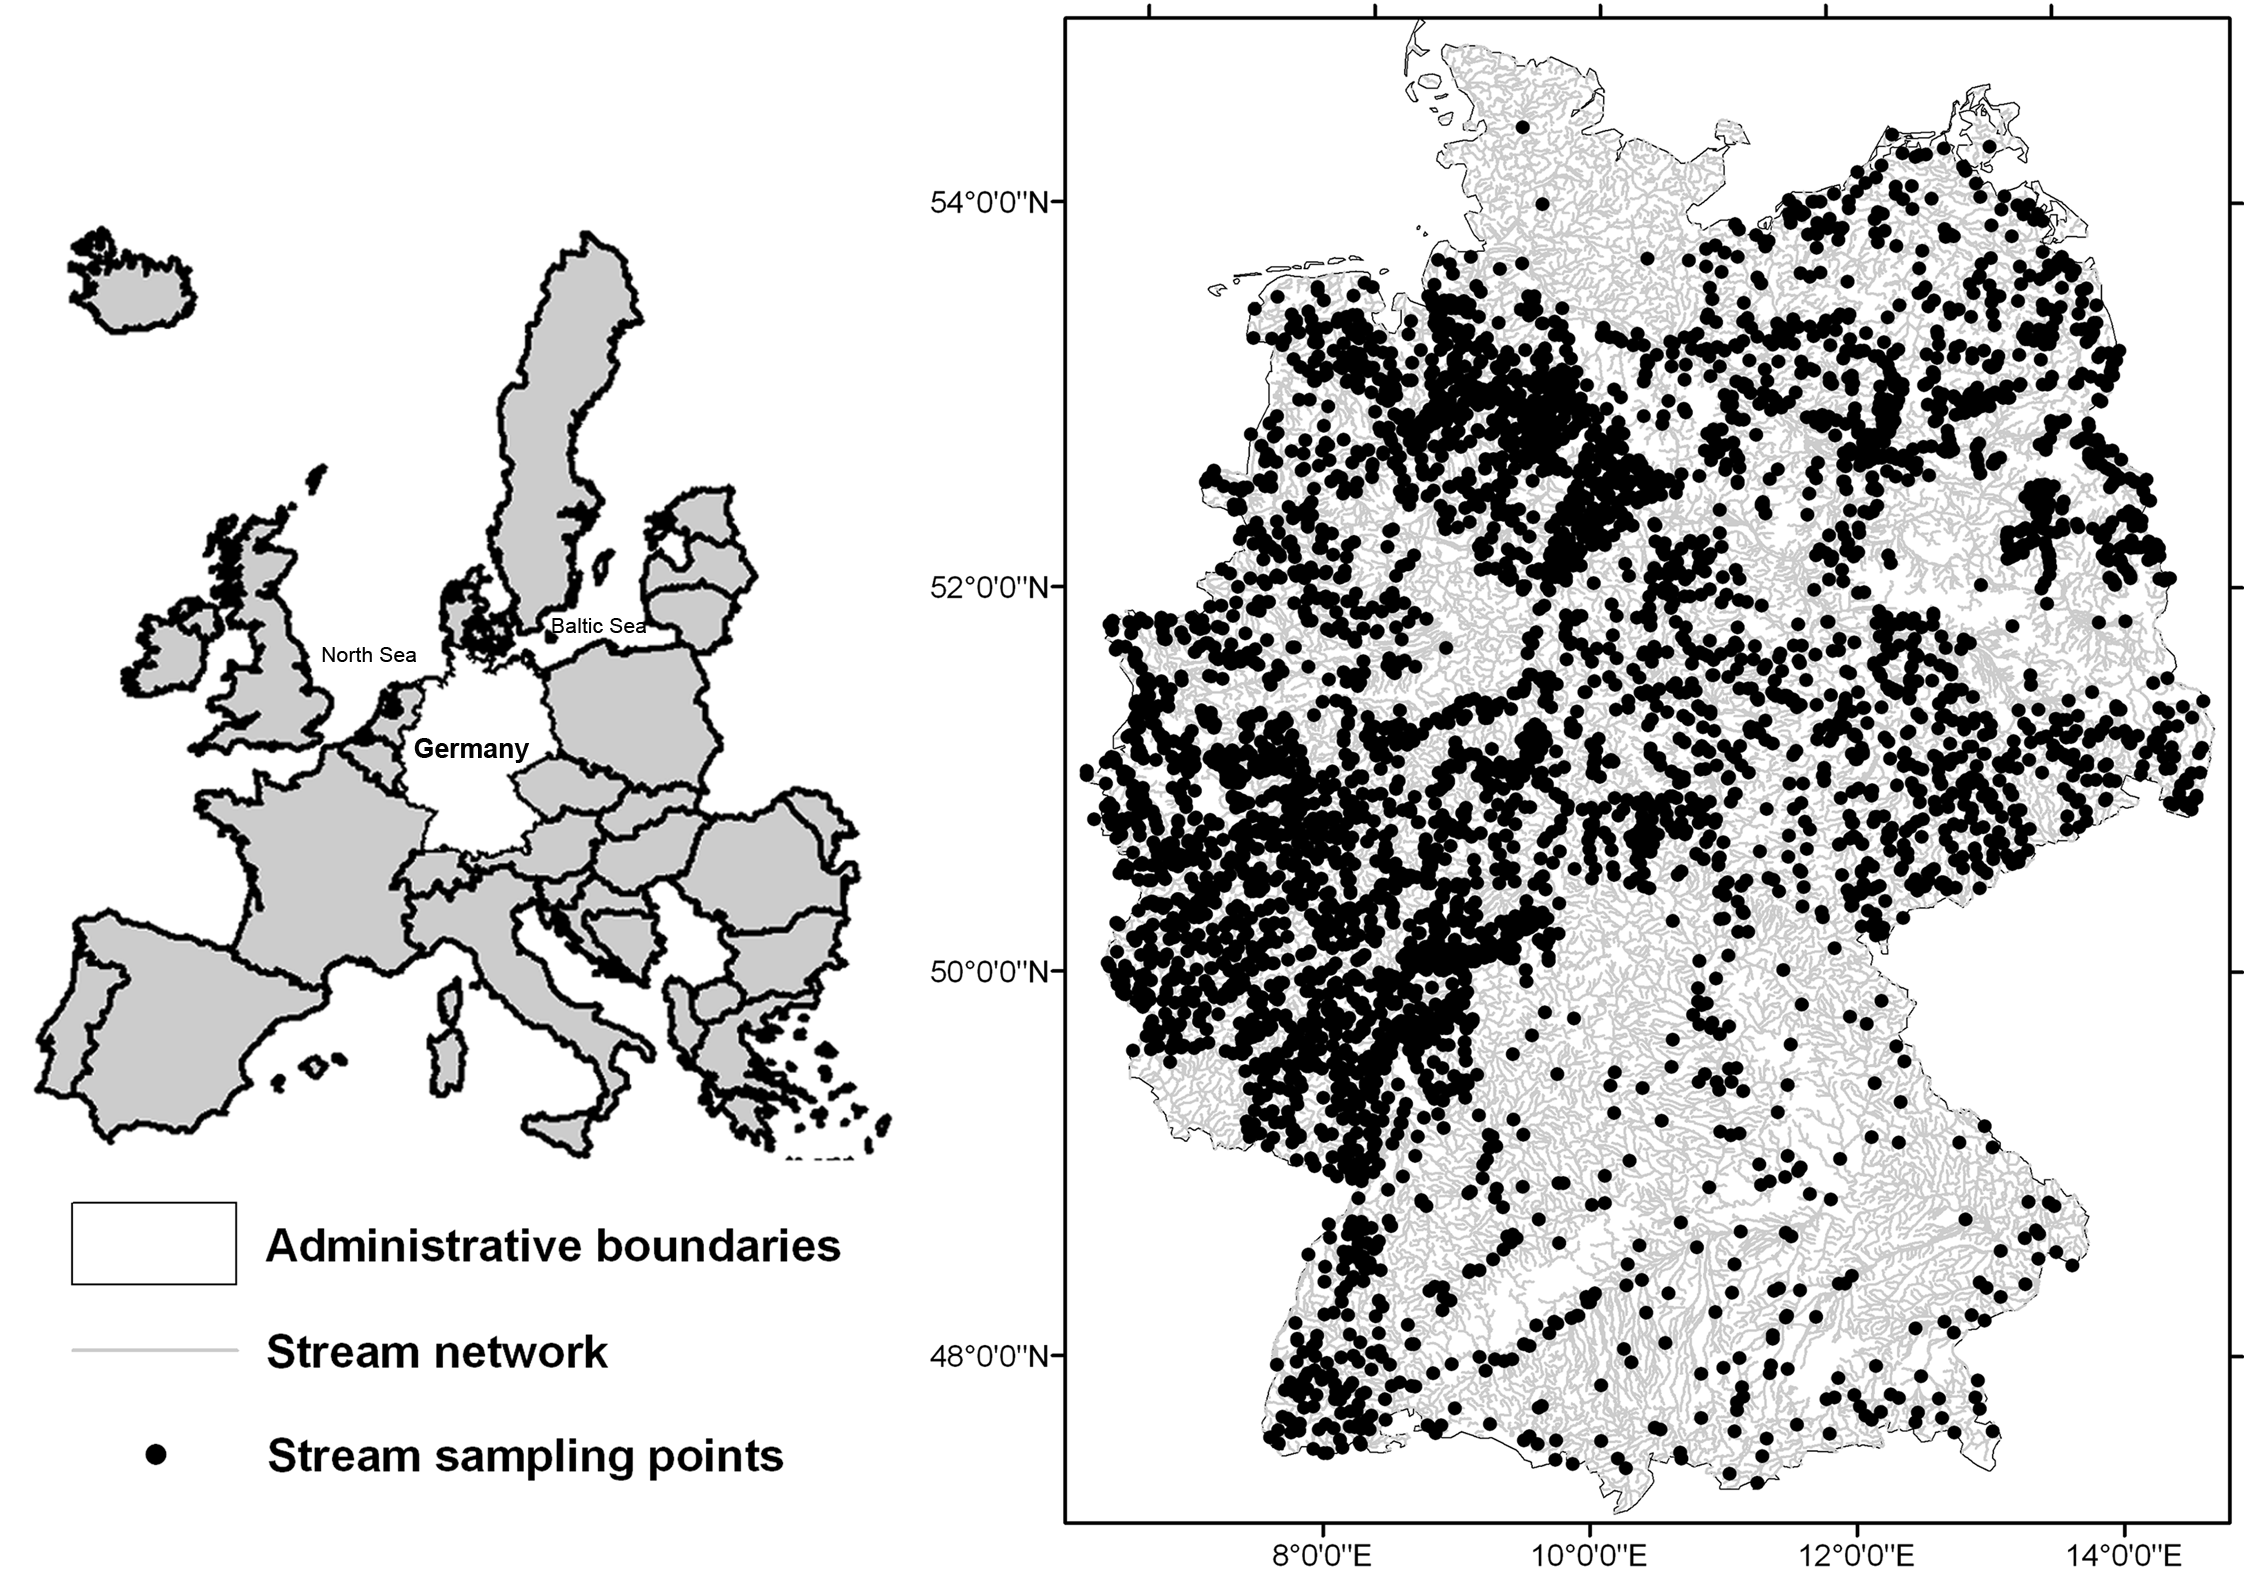
\includegraphics[width=\textwidth]{Figures/Fig_4_1.png}
  \caption{Distribution of the 4,752 stream sites sampled by the German national bio-monitoring program during 2006-2007. Spatial reference system is WGS 1984.}
  \label{Fig_4_1}
\end{figure}

We examined the homogeneity of taxonomic resolution and found that the organisms were reported at different taxonomic levels (from class to species). We took the subset of 1,901 organisms (91 \%) that were reported at genus (660) and species (1,241) levels. From this subset, we selected the aquatic insect orders, namely Diptera (True flies), Ephemeroptera (Mayflies), Odonata (Dragonflies and Damselflies), Plecoptera (Stoneflies) and Trichoptera (Caddisflies) (Table 4.1). Aerial dispersers are more suitable for large scale analyses than exclusive aquatic dispersers, because they can disperse through the landscape and are not limited to the stream network (Bonada et al., 2012; Wikelski et al., 2006). Moreover, these orders were also used in previous large scale studies to indicate climate vulnerability (Conti et al., 2013; Hering et al., 2009; Hershkovitz et al., 2015; Sandin et al., 2014; Tierno de Figueroa et al., 2010) and information for the selected traits were available for all organisms in these orders. This resulted in 782 species [and 395 genera] that comprised 384 [216] dipterans, 101 [39] ephemeropterans, 42 [33] odonates, 52 [36] plecopterans and 203 [71] trichopterans. Next, in case that a taxon was identified at genus level for more than 1 \% of stream sites, we converted all species belonging to this genus to genus level. This was the case for 73 \% of the species and was done to avoid artifacts from potential spatial pattern linked to the taxonomic resolutions, for instance mainly genus level identification in regions with low data coverage.

\subsubsection{Biological and ecological traits data}
\label{Biological and ecological traits data}

Biological and ecological traits of aquatic insects were taken from two databases: (i) the freshwater ecology database (\href{http://www.freshwaterecology.info}{www.freshwaterecology.info}) (Schmidt-Kloiber and Hering, 2015) and (ii) the Tachet database (Usseglio-Polatera et al., 2000). The trait information is recorded at species level in the freshwater ecology database, whereas they are recorded mostly at genus and species levels in the Tachet database. In both databases, the membership state (see Schmera et al. (2015) for terminology) of a taxon for a particular trait is generally described on a scale from zero to 10 (with exceptions for the Tachet database); zero indicates no membership and 10 the highest membership state. We selected the climate-associated traits from six grouping features (for details see Table 4.1) and converted the membership state of the traits into percentages as suggested by Schmera et al. (2015). These traits were selected because they were used in previous large scale studies to indicate vulnerability (Conti et al., 2013; Hering et al., 2009; Hershkovitz et al., 2015; Sandin et al., 2014; Tierno de Figueroa et al., 2010) and have the highest data coverage for the macroinvertebrates in German streams. We also compared the membership states of the insect orders for each of the selected traits (Table C.1 in appendix C).

\subsubsection{Calculation of assemblage trait composition}
\label{Calculation of assemblage trait composition}

The biomonitoring data were linked to the trait data using the codes of “The development and testing of an integrated assessment system for the ecological quality of streams and rivers throughout Europe using benthic macroinvertebrates” (AQEM) project to avoid discrepancies in naming conventions (Department of Applied Zoology/Hydrobiology, University Duisburg-Essen, Germany (DZHUDE), 2008). Each of the species was assigned with the  traits using their corresponding percentage membership states that were multiplied with the absolute abundance classes of the species for a site to compute relative abundance classes for the traits (Figure 4.2). To assign trait information to genera, we calculated the median of the related species level information following Schmidt-Kloiber and Nijboer (Schmidt-Kloiber and Nijboer, 2004) except for maximal body size where genus level information were available in the Tachet database for all genera. Subsequently, the assemblage trait composition, i.e. abundance weighted trait (AWT) was calculated following the procedure described in (Schmera et al., 2014) and as outlined in Figure 4.2. The AWT was calculated as a measure of assemblage trait composition because it is the most frequently used metric to assess the relationship between assemblage traits and environmental variables (Dolédec et al., 2006; Larsen and Ormerod, 2010). Note that we use the term assemblage trait composition to improve readability, although the assemblage data was restricted to aquatic insects, and hence does not represent the complete macroinvertebrate assemblage. The calculation resulted in annual averaged abundance-weighted traits (AWT) for each insect order (Figure C.1 in appendix C) and for the combined (full) data (Figure 4.3; 4.4) for each stream site. The calculation was omitted for the dispersal capacity of ephemeropterans and plecopterans because the grouping feature consisted of only one trait (low dispersal). However, they were included in the calculation for the full data.

\subsubsection{Bioclimatic indices and altitude data}
\label{Bioclimatic indices and altitude data}

The 35 bioclimatic indices (BI, denoted as “Bio01” to “Bio35”, see Table 4.2 for details) for temperature, precipitation, radiation and moisture were collected from the global climatologies for bioclimatic modeling (CliMond) database (www.climond.org) (Kriticos et al., 2012). A previous study showed that these BIs can provide an approximation of climate impact on assemblage patterns, despite the omission of confounding endogenous factors such as biotic interactions, evolutionary change and dispersal potential (Araújo and Peterson, 2012). The scale of variability was determined by the spatial resolution of the BI raster, which is 10 arc-minutes (approximately 18 km). The digital elevation model (giving altitude over mean sea level) for Germany was collected from the ASTER GDEM on one arc-second (approximately 30 m) resolution (National Aeronautics and Space Administration (NASA) and Japan’s Ministry of Economy, Trade and Industry (METI), 2009). The altitude raster was resampled to the resolution of the BI rasters to extract altitude information for each BI raster cell.

\begin{figure}[h!]
  \centering
  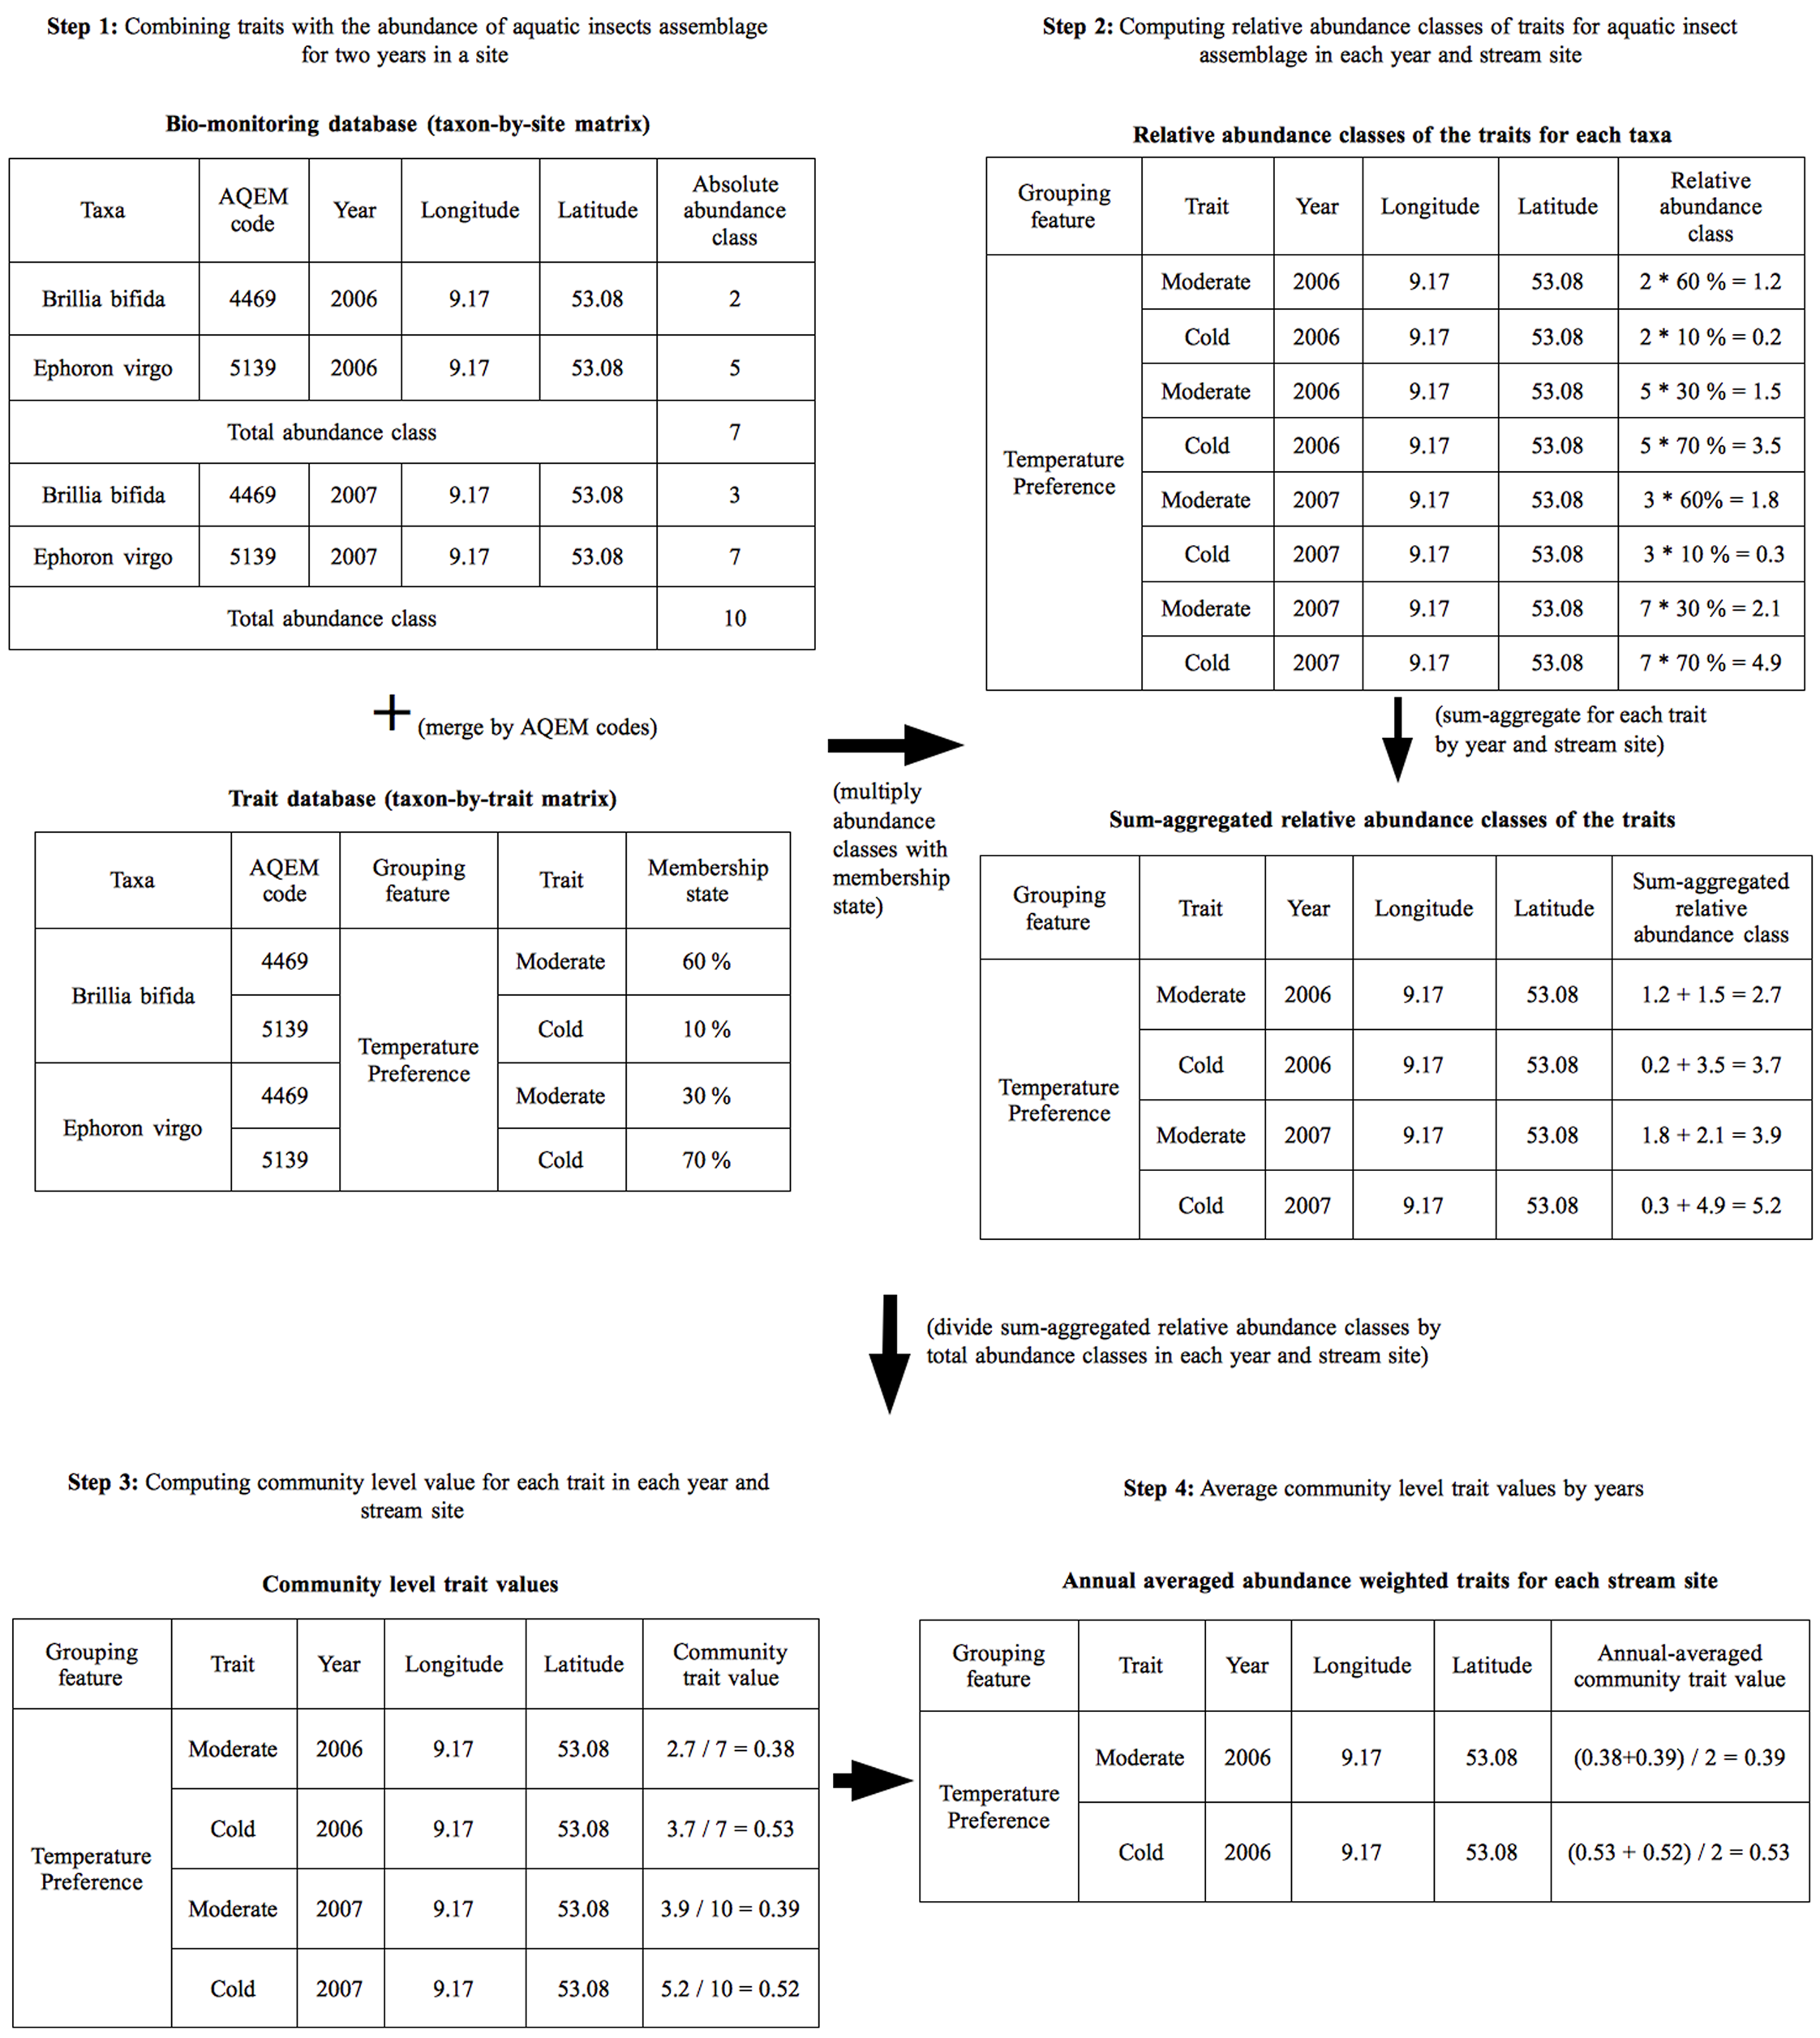
\includegraphics[width=0.8\linewidth]{Figures/Fig_4_2.png}
  \caption{Conversion steps from abundance classes of the selected aquatic insects to trait compositional (annual averaged abundance weighted traits) data.}
  \label{Fig_4_2}
\end{figure}

Although no clear gradient in the BIs was found for Germany, lower temperatures and higher precipitation were mostly observed in the southern regions, whereas higher temperatures and lower precipitation were mostly observed in the northern regions (Figure C.2). For example, observed ranges of the annual mean temperature (Bio01) and annual precipitation (Bio12) are 2 to 5 \textsuperscript{0}C and 7 to 12 \textsuperscript{0}C, and 1200 to 1600 mm and 600 to 800 mm in the southern and northern regions, respectively. The northern and southern regions are portrayed as flat (zero to 250 m above sea level) and mountainous (600 to 1800 m above sea level), respectively (Figure C.3).  The BIs showed significant (p $<$ 0.001) spatial autocorrelation, i.e. average Moran's I = 0.28 (Table C.2). Significant spatial gradients were also observed for the BIs (Table C.2). Longitudinal (North – South) and altitudinal (high – low) gradients were both stronger than the latitudinal gradient (East – West) for

\begin{landscape}
\small
\setlength{\LTcapwidth}{\linewidth}
\begin{longtable}[c]{>{\centering\arraybackslash}m{3.2cm}|>{\centering\arraybackslash}m{0.7cm}>{\centering\arraybackslash}m{1.7cm}>{\centering\arraybackslash}m{0.8cm}>{\centering\arraybackslash}m{1.0cm}>{\centering\arraybackslash}m{1.1cm}>{\centering\arraybackslash}m{1.3cm}|>{\centering\arraybackslash}m{0.7cm}>{\centering\arraybackslash}m{1.7cm}>{\centering\arraybackslash}m{0.8cm}>{\centering\arraybackslash}m{1.0cm}>{\centering\arraybackslash}m{1.1cm}>{\centering\arraybackslash}m{1.3cm}}
\caption{Explained variances and spatial autocorrelation in the traits of each order and full data by the bioclimatic indices. The detailed information on the traits including the source databases and their occurrence and variability in Germany are presented. \label{Table 4.1}}\\

\hline
\textbf{Grouping features and traits} & \multicolumn{6}{c|}{\textbf{Explained variability (\%)}} & \multicolumn{6}{c}{\textbf{Explained spatial autocorrelation (\%)}}\\
 & \textbf{Diptera} & \textbf{Ephemeroptera} & \textbf{Odonata} & \textbf{Plecoptera} & \textbf{Trichoptera} & \textbf{Full data} & \textbf{Diptera} & \textbf{Ephemeroptera} & \textbf{Odonata} & \textbf{Plecoptera} & \textbf{Trichoptera} & \textbf{Full data}\\
\hline
\endfirsthead

\hline
\textbf{Grouping features and traits} & \multicolumn{6}{c|}{\textbf{Explained variability (\%)}} & \multicolumn{6}{c}{\textbf{Explained spatial autocorrelation (\%)}}\\
 & \textbf{Diptera} & \textbf{Ephemeroptera} & \textbf{Odonata} & \textbf{Plecoptera} & \textbf{Trichoptera} & \textbf{Full data} & \textbf{Diptera} & \textbf{Ephemeroptera} & \textbf{Odonata} & \textbf{Plecoptera} & \textbf{Trichoptera} & \textbf{Full data}\\
\hline
\endhead

\hline
\endfoot

\hline
\textbf{\textit{Average over traits and orders}} & \textbf{\textit{14}} & \textbf{\textit{16\textsuperscript{\#}}} & \textbf{\textit{13}} & \textbf{\textit{16\textsuperscript{\#}}} & \textbf{\textit{15}} & \textbf{\textit{19}} & \textbf{\textit{50}} & \textbf{\textit{59\textsuperscript{\#}}} & \textbf{\textit{46}} & \textbf{\textit{53}} & \textbf{\textit{54}} & \textbf{\textit{59}}\\
\hline
\endlastfoot

\textbf{Biological traits} & & & & & & & & & & & & \\
 & & & & & & & & & & & & \\
\textit{Dispersal capacity\textsuperscript{a}} & & & & & & & & & & & & \\
Unknown & NA & NA & NA & NA & 4.7 & 4.1 & NA & NA & NA & NA & 44 & 25\\
Low & NA & * & NA & * & 12 & 16 & NA & * & NA & * & 38 & 68\\
High & NA & NA & NA & NA & 10 & 15 & NA & NA & NA & NA & 54 & 38\\
\textit{Average} & \textit{NA} & \textit{NA} & \textit{NA} & \textit{NA} & \textit{9.1} & \textit{12} & \textit{NA} & \textit{NA} & \textit{NA} & \textit{NA} & \textit{45} & \textit{44}\\
\hline
\textit{Maximal body size\textsuperscript{b}} & & & & & & & & & & & & \\
$>$ 0.25 cm to 0.5 cm & 8.0 & 10 & NA & 32 & 19 & 17 & 1.0 & 35 & NA & 79 & 51 & 78\\
$>$ 0.5 cm to 1 cm & 14 & 13 & NA & 9.7 & 11 & 12 & 62 & 61 & NA & 83 & 50 & 65\\
$>$ 1 cm to 2 cm & 10 & 12 & 18 & 21 & 14 & 18 & 41 & 35 & 32 & 49 & 60 & 75\\
$>$ 2 cm to 4 cm & 16 & 12 & 10 & 8.6 & 12 & 14 & 39 & 80 & 88 & 26 & 26 & 65\\
$>$ 4 cm to 8 cm & 13 & NA & 16 & NA & NA & 13 & 3.0 & NA & 11 & NA & NA & 46\\
\textit{Average} & \textit{12} & \textit{12} & \textit{15} & \textit{18} & \textit{14} & \textit{15} & \textit{29} & \textit{53} & \textit{44} & \textit{59} & \textit{47} & \textit{66} \\
\hline
\textit{Reproductive capacity\textsuperscript{a}} & & & & & & & & & & & & \\
Flexible & NA & 23 & NA & 25 & 4.1 & 10 & NA & 66 & NA & 90 & 65 & 37\\
Semivoltine & 11 & 10 & NA & 7.0 & 22 & 14 & 55 & 29 & NA & 42 & 52 & 47\\
Univoltine & 16 & 9.3 & NA & 14 & 28 & 8.6 & 53 & 70 & NA & 89 & 68 & 60\\
Bivoltine & 12 & 11 & NA & NA & 15 & 20 & 35 & 70 & NA & NA & 11 & 71\\
Trivoltine & 7.6 & 25 & NA & NA & NA & 9.7 & 2.3 & 60 & NA & NA & NA & 34\\
Multivoltine & 17 & 15 & NA & NA & 3.3 & 9.1 & 76 & 41 & NA & NA & 36 & 16\\
\textit{Average} & \textit{13} & \textit{15} & \textit{NA} & \textit{15} & \textit{14} & \textit{12} & \textit{44} & \textit{56} & \textit{NA} & \textit{74} & \textit{46} & \textit{44}\\
\hline
\textit{Resistance to drought\textsuperscript{a}} & & & & & & & & & & & & \\
Unknown resistance type & NA & NA & NA & 18 & 8.2 & 10 & NA & NA & NA & 3.7 & 92 & 51\\
No drought resilience & NA & NA & NA & NA & 13 & 7.9 & NA & NA & NA & NA & 28 & 0.1\\
Egg diapause & NA & 17 & NA & 18 & NA & 41 & NA & 61 & NA & 46 & NA & 73\\
Larvae diapause & NA & 16 & NA & NA & 6.1 & 13 & NA & 67 & NA & NA & 60 & 66\\
Adult diapause & NA & NA & NA & NA & 11 & 13 & NA & NA & NA & NA & 18 & 15\\
\textit{Average} & \textit{NA} & \textit{16} & \textit{NA} & \textit{18} & \textit{9.8} & \textit{17} & \textit{NA} & \textit{64} & \textit{NA} & \textit{25} & \textit{49} & \textit{41}\\
\hline
\textbf{Ecological traits} & & & & & & & & & & & & \\
 & & & & & & & & & & & & \\
\textit{Current preference\textsuperscript{a}} & & & & & & & & & & & & \\
Indifferent & 9.2 & NA & NA & 18 & 5.3 & 24 & 33 & NA & NA & 63 & 2.7 & 67\\
Limnobiont & 6.3 & NA & 9.8 & NA & 22 & 15 & 22 & NA & 42 & NA & 65 & 61\\
Limnophil & 7.1 & 25 & 6.5 & 27 & 43 & 41 & 90 & 56 & 5.6 & 63 & 75 & 77\\
Limno to Rheophil & 5.1 & 4.4 & 12 & 8.7 & 15 & 8.1 & 12 & 42 & 13 & 36 & 57 & 74\\
Rheo to Limnophil & 12 & 15 & 14 & 7.3 & 6.7 & 13 & 52 & 58 & 63 & 13 & 82 & 71\\
Rheophil & 27 & 17 & 20 & 34 & 26 & 40 & 69 & 58 & 67 & 72 & 68 & 85\\
Rheobiont & 21 & 7.3 & 8.7 & 13 & 22 & 30 & 52 & 13 & 89 & 65 & 54 & 59\\
\textit{Average} & \textit{13} & \textit{14} & \textit{12} & \textit{18} & \textit{20} & \textit{25} & \textit{47} & \textit{45} & \textit{47} & \textit{52} & \textit{58} & \textit{71}\\
\hline
\textit{Temperature preference\textsuperscript{a}} & & & & & & & & & & & & \\
Eurytherm & 26 & 21 & NA & 22 & 14 & 34 & 84 & 65 & NA & 67 & 66 & 87\\
Very cold & 8.9 & 34\textsuperscript{\#} & NA & 16 & 17 & 50\textsuperscript{\#} & 83 & 76 & NA & 34 & 59 & 82\\
Cold & 30 & 14 & NA & 8.5 & 19 & 42 & 71 & 84 & NA & 65 & 69 & 91\textsuperscript{\#}\\
Moderate & 15 & 33 & NA & 6.9 & 8.5 & 8.6 & 84 & 88 & NA & 67 & 98\textsuperscript{\#} & 60\\
Warm & 24 & 15 & NA & 10 & 15 & 24 & 82 & 80 & NA & 16 & 66 & 86\\
\textit{Average} & \textit{21} & \textit{23} & \textit{NA} & \textit{13} & \textit{15} & \textit{32\textsuperscript{\#}} & \textit{81} & \textit{79} & \textit{NA} & \textit{50} & \textit{71} & \textit{81\textsuperscript{\#}} \\
 & & & & & & & & & & & & \\

\end{longtable}
\vspace{-0.4cm}
\hspace{-0.6cm}
\footnotesize
\textsuperscript{a}data source: freshwater ecology database (www.freshwaterecology.info) (Schmidt-Kloiber & Hering, 2012)\\
\textsuperscript{b}data source: Tachet database (Usseglio-Polatera et al., 2000)\\
\textsuperscript{NA}Trait not occurring\\
*Trait omitted from the analysis because of zero variability (i.e. all organisms have same trait) and therefore the abundance weighted trait cannot be computed\\
\textsuperscript{\#}Traits and orders showing the strongest relationship with the bioclimatic indices in their variability and spatial autocorrelation\\

\normalsize
\vspace{1cm}

\noindent most of the BIs. Longitude and altitude of the BI cells showed significantly high correlation (r = -0.8, p $<$ 0.001) with each other and thus indicates that the dominant climatic variation along the North – South (longitudinal) gradient on the scale of Germany (also observed in Figure C.2) may be attributed to topography, i.e. altitude (low – high).

\newpage

\begin{figure}[t]
  \centering
  \vspace{-1.5cm}
  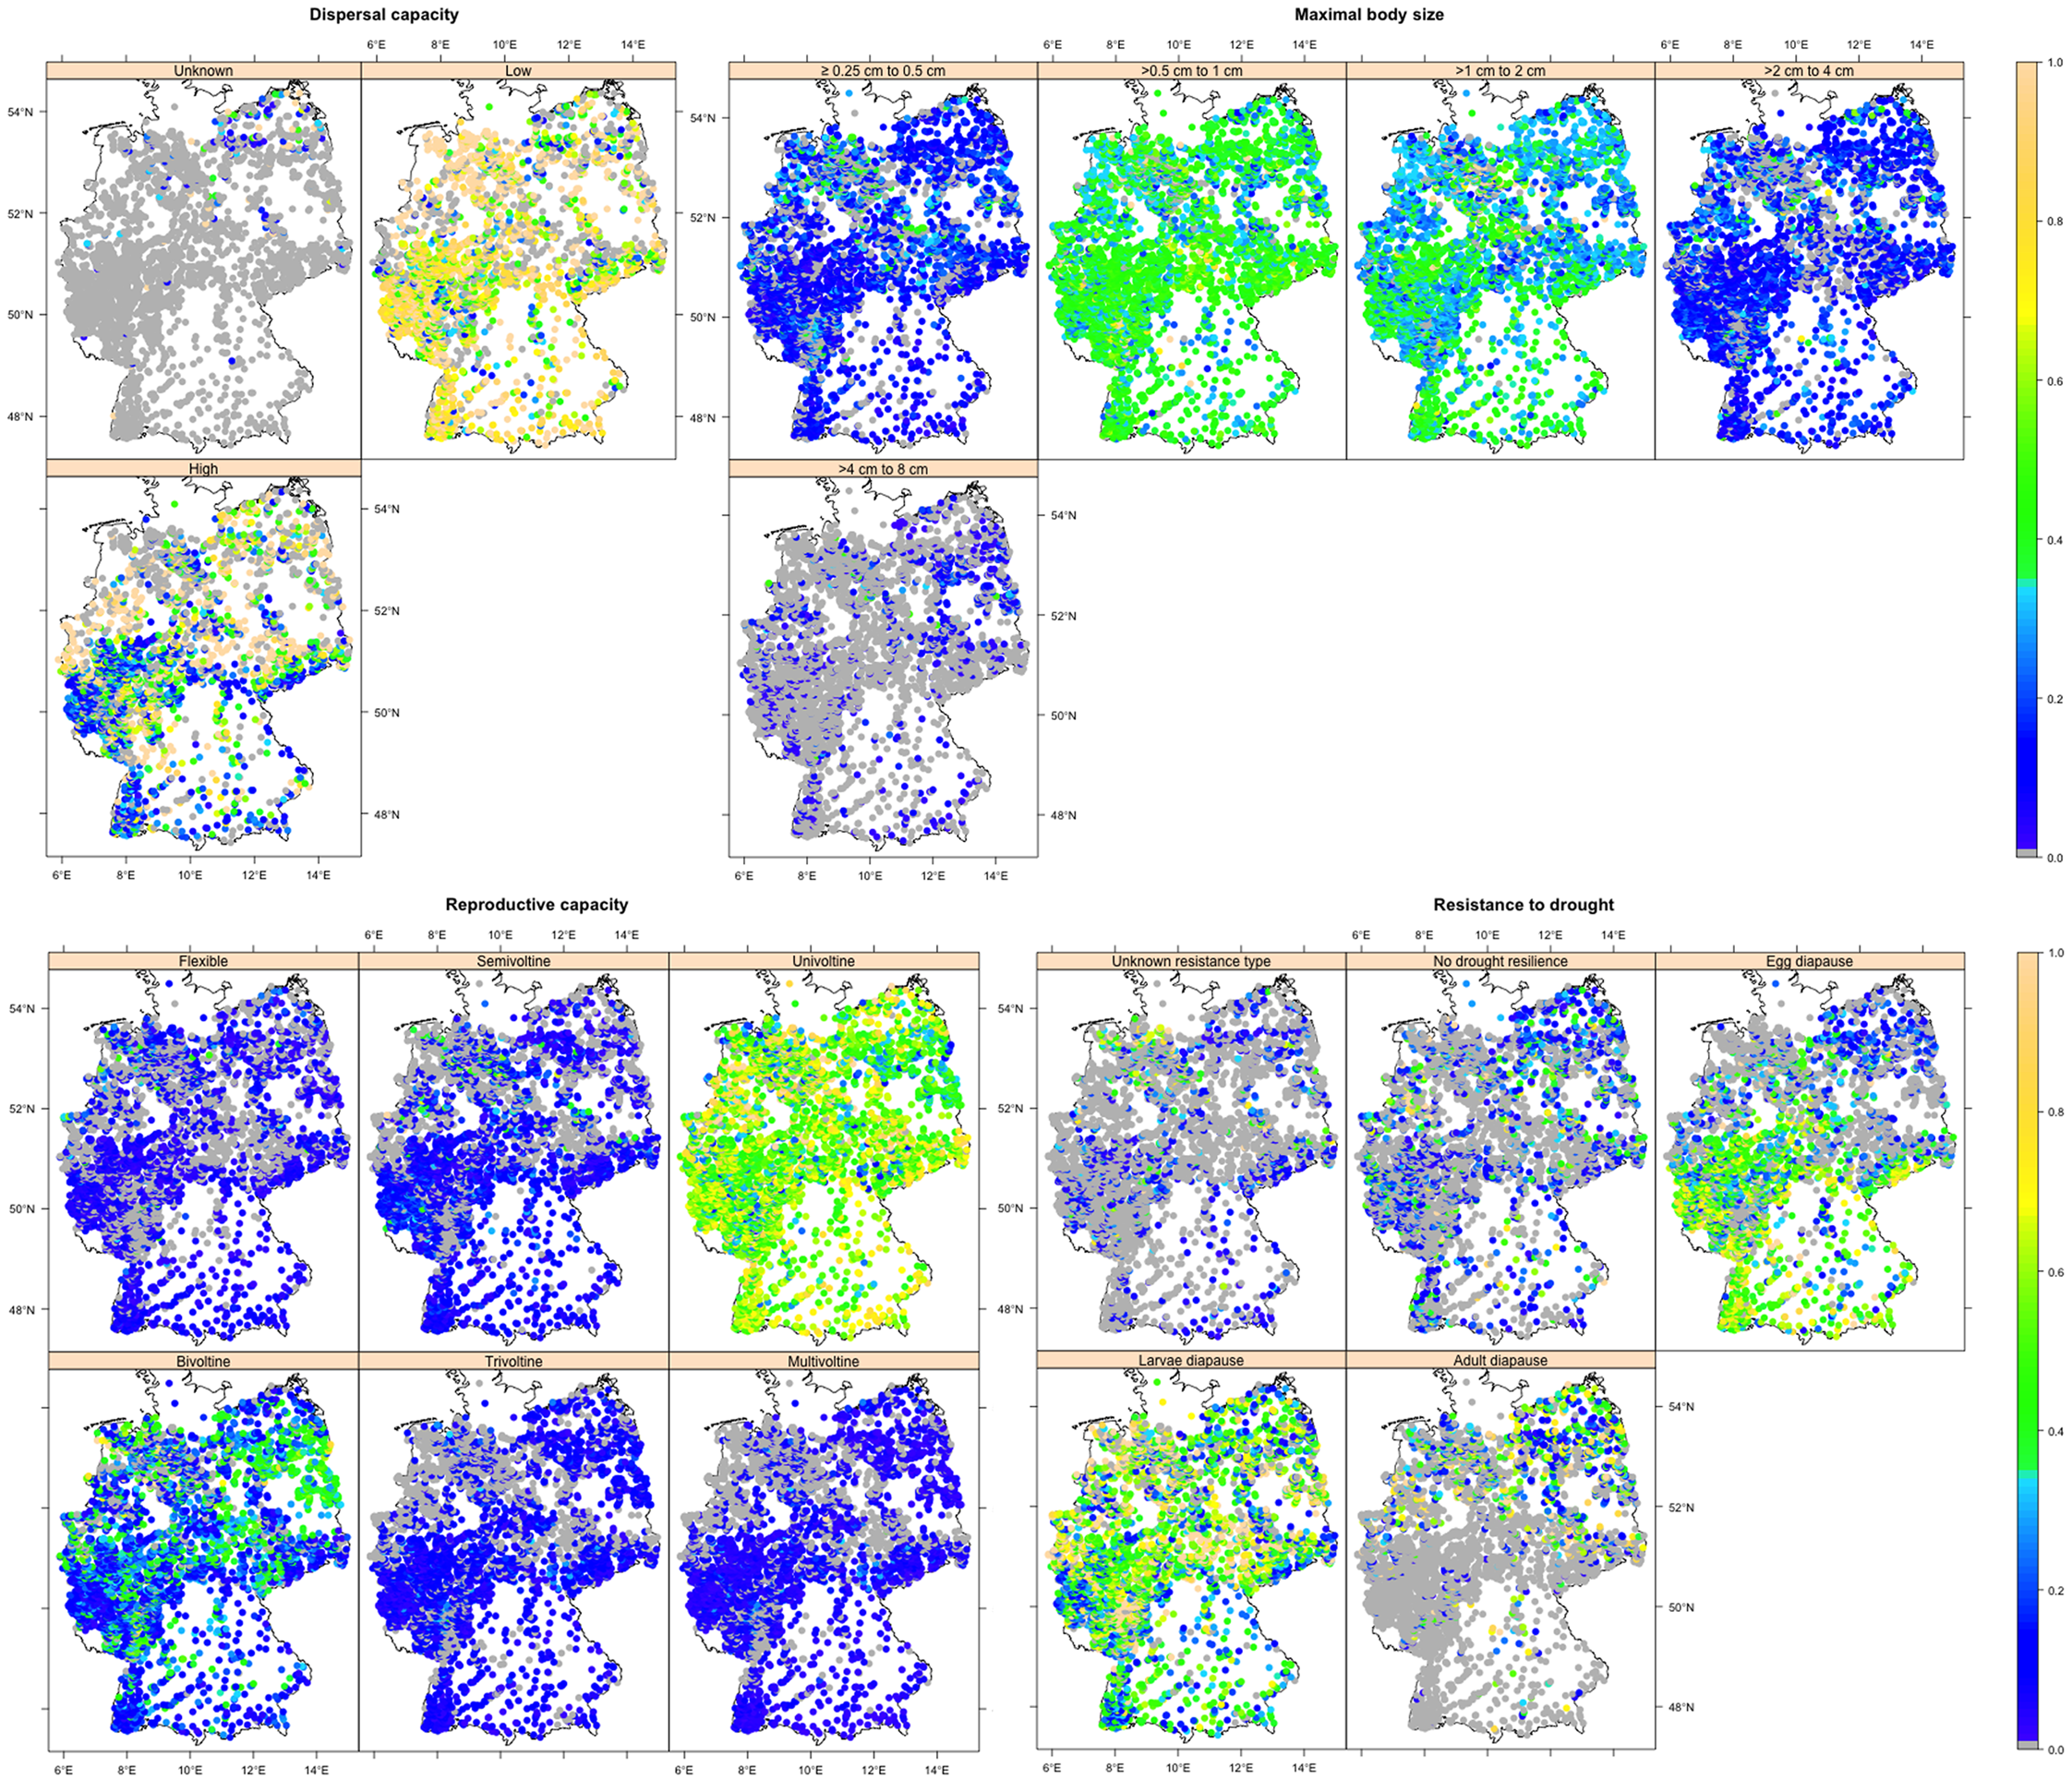
\includegraphics[width=0.8\linewidth]{Figures/Fig_4_3.png}
  \caption{Annual averaged abundance weighted traits across 4,752 stream sites in Germany for the biological traits of the full data. The figure sub-captions and panel captions indicate names of grouping features and traits, respectively. The gray dots indicate the zero abundance, i.e. trait absence.}
  \label{Fig_4_3}
\end{figure}

\newpage

\begin{figure}[t]
  \centering
  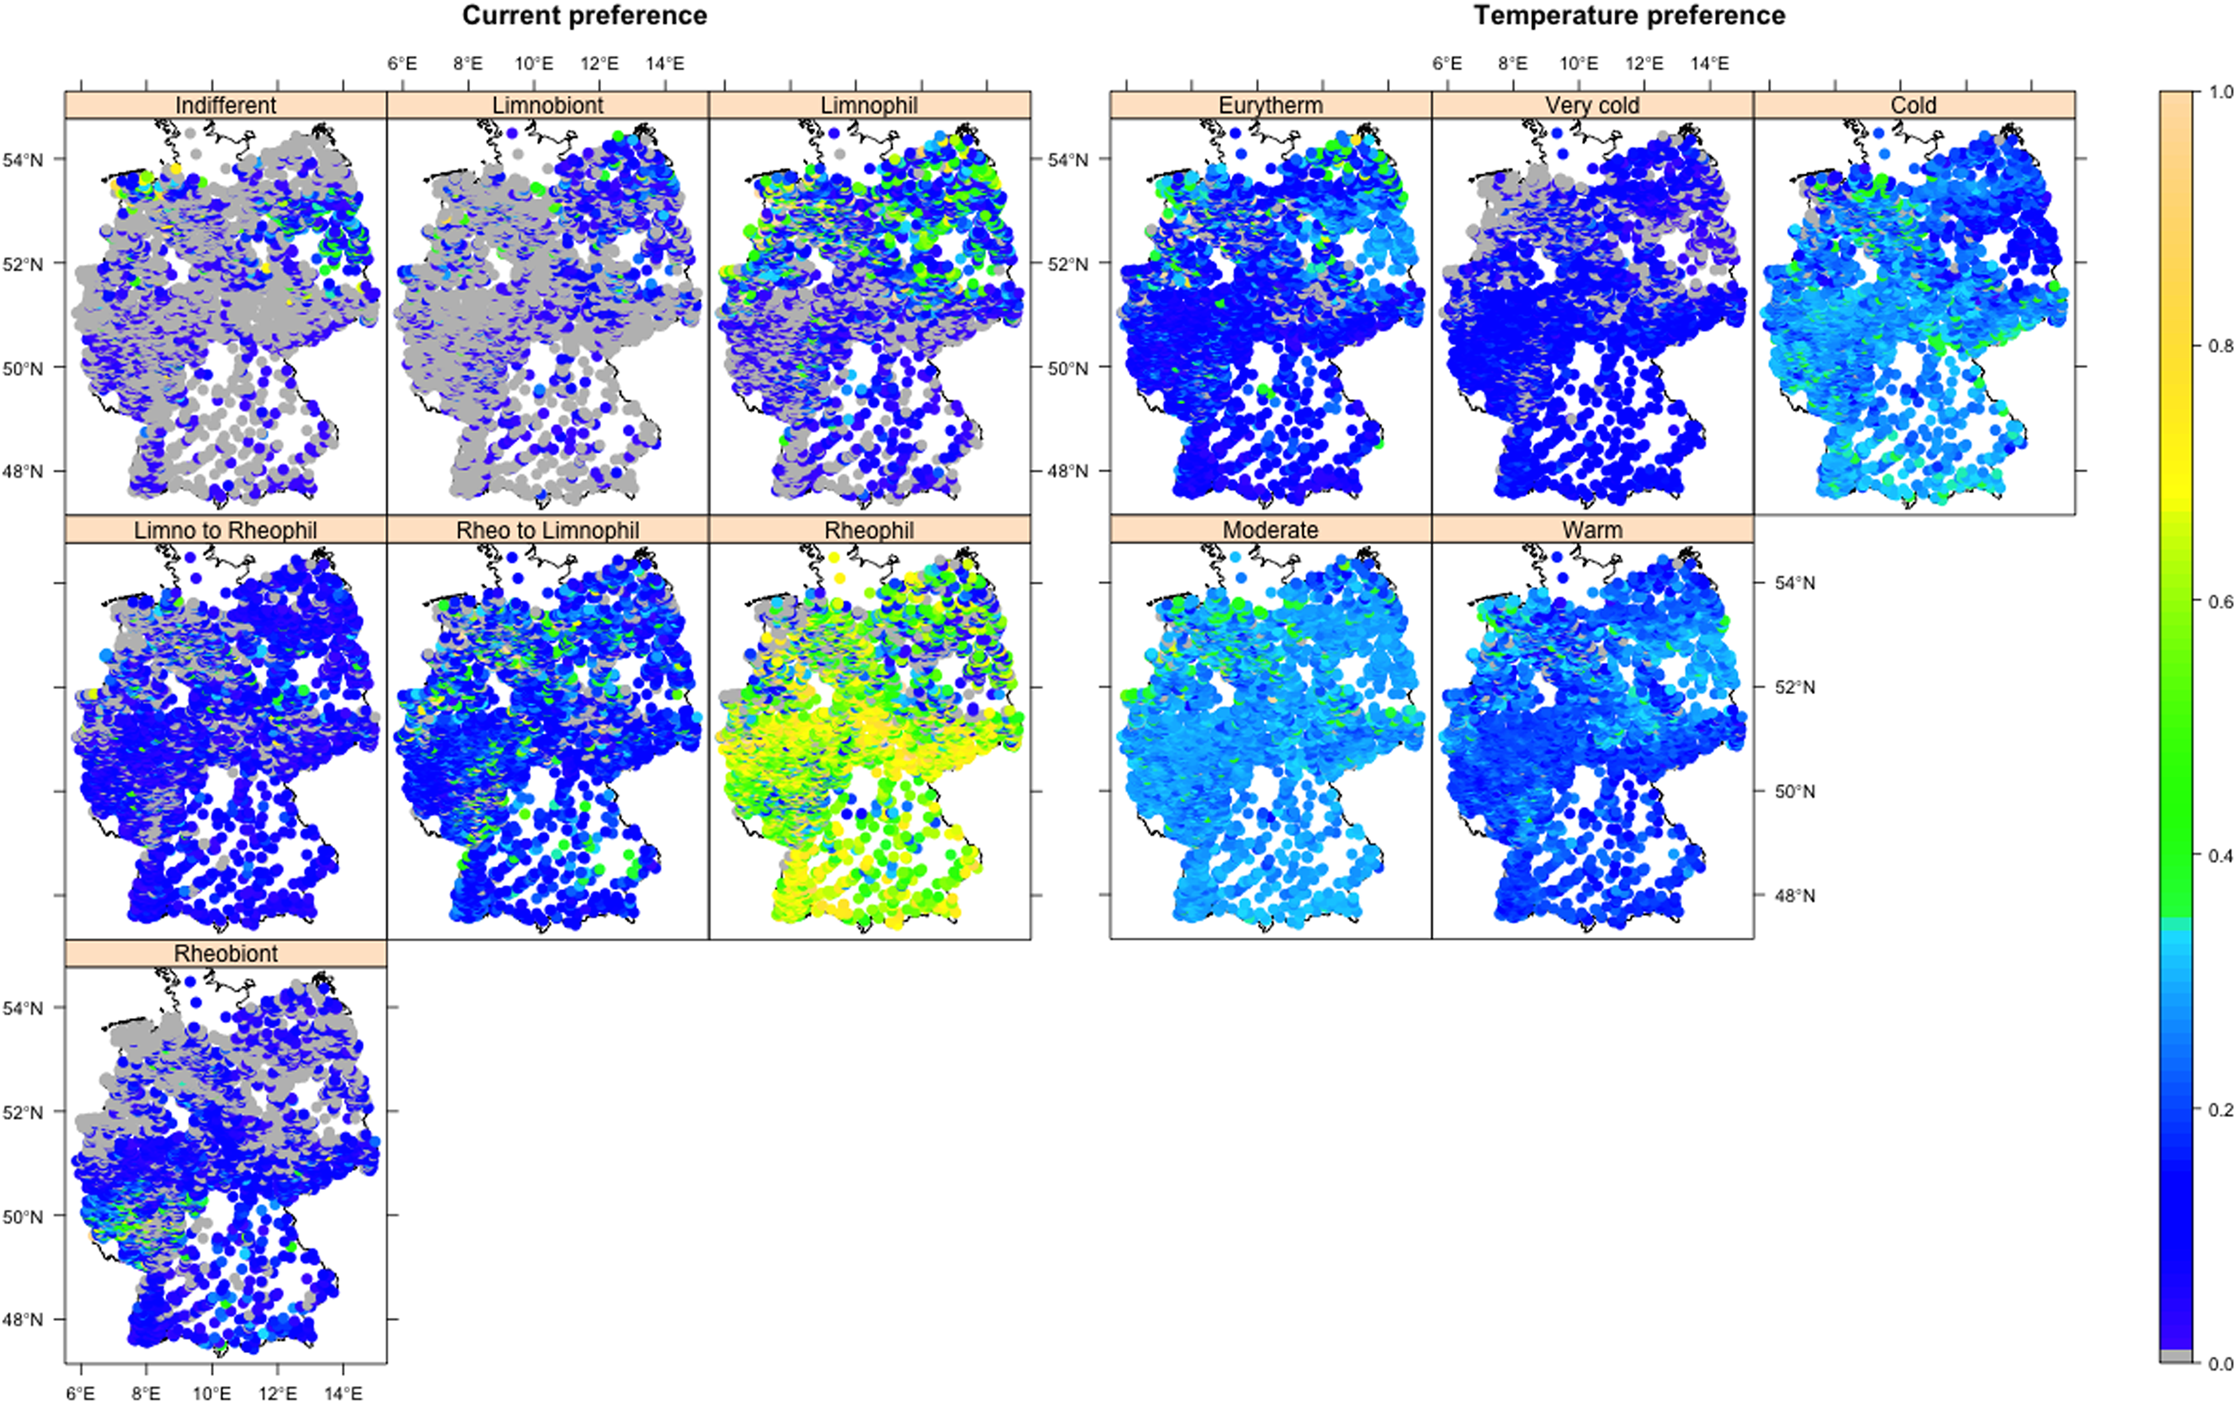
\includegraphics[width=\linewidth]{Figures/Fig_4_4.png}
  \caption{Annual averaged abundance weighted traits across 4,752 stream sites in Germany for the ecological traits of the full data. The figure sub-captions and panel captions indicate names of grouping features and traits, respectively. The gray dots indicate the zero abundance, i.e. trait absence.}
  \label{Fig_4_4}
\end{figure}

\end{landscape}

\subsubsection{Pre-processing of BI and AWT data}
\label{Pre-processing of BI and AWT data}

The stream sites covered 72\% of the total BI raster cells within the boundary of Germany (Figure C.4). However, given the relatively coarse resolution of the BI data, multiple sites were often located in one BI raster cell. Therefore, we aggregated the AWTs in all sites within a BI raster cell via averaging and assigned the result to that cell to avoid pseudo replication. The BIs exhibited considerable multicollinearity (Figure C.5) and therefore we conducted a principal component analysis (PCA) to arrive at independent variables and extracted the scores of the 35 orthogonal principal components, as suggested by Graham (2003), for latter analysis. PCA was preferred over residual and sequential regression as this also obliterates the likely effects of the latent spatial variables (as described above) on the BIs (Graham, 2003). All data processing and PCA of BIs were done in R software environment (R Development Core Team, 2015) using the packages “sp” (Bivand et al., 2008), “vegan” (Oksanen et al., 2007), “raster” (Hijmans and Van Etten, 2010) and “maptools” (Lewin-Koh et al., 2011).

\subsection{Analyses of the spatial relationship between traits and climate}
\label{Analyses of the spatial relationship between traits and climate}

The spatial relationship between the aggregated AWT per BI cell and the BIs was analyzed in four steps (Figure C.6). First, we checked for spatial autocorrelations in the AWT (Table C.3). The spatial autocorrelation was analyzed using Global Moran's I (see Bonada et al. (2012) for details on computation), where great circle distances among BI cell pairs were given as weights based on the simplified assumption that the selected species disperse symmetrically during their terrestrial life stage (Wikelski et al., 2006). The computations of spatial autocorrelations were done using the R package “ape” (Paradis et al., 2004).

Second, zero-or-one inflated beta regression models were fitted with the AWT as response and 35 principal component scores of the BIs as explanatory variables (Ospina and Ferrari, 2012). This was done to identify the traits and insect orders with the highest climate response. We used zero-or-one inflated beta regression because the response variables were proportional data and included many zeros and ones (Nishii and Tanaka, 2012). The models were fitted for the AWT of each order and the full data and the adjusted R\textsuperscript{2}s were calculated to identify the explained variance by the BIs. The zero-or-one-inflated beta regression model fitting was done using the R package “gamlss” (Rigby and Stasinopoulos, 2005).

In the third step, we checked for spatial autocorrelation in the residuals of the trait-climate models using Moran's I as outlined above. The Moran's I values for the residuals of the trait-climate models were subtracted from the complete Moran's I values for the AWT (computed at the first step). Thus, the percentage of trait spatial autocorrelation that is associated with the BIs was identified. This was done to identify the traits and orders that show the highest potential for changing their distributional pattern, i.e. redistribution under future climate change.

In a final step, the zero-or-one inflated beta regression models were re-fitted with the AWT for the previously identified traits and orders with the highest climate response and potential for redistribution as response variables and 35 BIs (original values) separately as explanatory variables. The BIs with the highest explanatory power in terms of R\textsuperscript{2} were identified for the traits and insect orders with the highest climate response. To identify the BIs explaining the highest amount of spatial autocorrelation in the traits and in the insect orders with the highest potential for redistribution, we computed the Moran's I in the residuals of the trait-individual BI models and subtracted them from the complete Moran's I computed at the first step.

\begin{landscape}
\small
\setlength{\LTcapwidth}{\linewidth}

\begin{longtable}[c]{>{\centering\arraybackslash}m{2.3cm}>{\centering\arraybackslash}m{5.5cm}|>{\centering\arraybackslash}m{3.0cm}>{\centering\arraybackslash}m{3.4cm}|>{\centering\arraybackslash}m{2.5cm}>{\centering\arraybackslash}m{3.0cm}}
\caption{Explained variances and spatial autocorrelation by the individual bioclimatic indices in the traits and orders with the highest climate response and potential for changing distribution pattern. Details on the bioclimatic variables are extracted from Kriticos et al. (2012) and \href{https://www.climond.org/Resources.aspx}{https://www.climond.org/Resources.aspx}. \label{Table 4.2}}\\

\hline
\textbf{Variable Number} & \textbf{Variables (unit)} & \multicolumn{2}{c|}{\textbf{Explained variance (\%)}} & \multicolumn{2}{c}{\textbf{Explained spatial autocorrelation (\%)}}\\
 & & \textbf{Very cold temperature preferring insects} & \textbf{Very cold temperature  preferring Ephemeroptera} & \textbf{Cold temperature preferring insects} & \textbf{Moderate temperature preferring Trichoptera}\\
\hline
\endfirsthead

\hline
\textbf{Variable Number} & \textbf{Variables (unit)} & \multicolumn{2}{c|}{\textbf{Explained variance (\%)}} & \multicolumn{2}{c}{\textbf{Explained spatial autocorrelation (\%)}}\\
 & & \textbf{Very cold temperature preferring insects} & \textbf{Very cold temperature  preferring Ephemeroptera} & \textbf{Cold temperature preferring insects} & \textbf{Moderate temperature preferring Trichoptera}\\
\hline
\endhead

\hline
\endfoot

\hline
\endlastfoot

Bio01 & Annual mean temperature (\textsuperscript{0}C) & 8.6 & 9.1 & 3.2 & 61\\
Bio02 & Mean diurnal temperature range (\textsuperscript{0}C) & 3.2 & 1.6 & 24 & 57\\
Bio03 & Isothermality & 7.2 & 2.9 & 26 & 50\\
Bio04 & Temperature seasonality & 2.8 & 0.9 & 5.9 & 61\\
Bio05 & Max temperature of warmest week (\textsuperscript{0}C) & 6.1 & 5.8 & 11 & 63\\
Bio06 & Min temperature of coldest week (\textsuperscript{0}C) & 1.8 & 3.5 & 6.1 & 59\\
Bio07 & Temperature annual range (\textsuperscript{0}C) & 0.5 & 0.1 & 6.6 & 61\\
Bio08 & Mean temperature of wettest quarter (\textsuperscript{0}C) & 5.3 & 4.2 & 3.1 & 59\\
Bio09 & Mean temperature of driest quarter (\textsuperscript{0}C) & 0.2 & 0.7 & 11 & 64\\
Bio10 & Mean temperature of warmest quarter (\textsuperscript{0}C) & 13 & 12 & 8.2 & 59\\
Bio11 & Mean temperature of coldest quarter (\textsuperscript{0}C) & 1.5 & 3.4 & 9.7 & 63\\
Bio12 & Annual precipitation (mm) & 15 & 13 & 29 & 37\\
Bio13 & Precipitation of wettest week (mm) & 13 & 11 & 31 & 36\\
Bio14 & Precipitation of driest week (mm) & 18\textsuperscript{\#} & 14 & 32 & 33\\
Bio15 & Precipitation seasonality & 1.4 & 0.5 & 5.3 & 63\\
Bio16 & Precipitation of wettest quarter (mm) & 13 & 11 & 28 & 41\\
Bio17 & Precipitation of driest quarter (mm) & 15 & 12 & 27 & 40\\
Bio18 & Precipitation of warmest quarter (mm) & 12 & 11 & 25 & 45\\
Bio19 & Precipitation of coldest quarter (mm) & 12 & 10 & 18 & 54\\
Bio20 & Annual mean radiation (W m\textsuperscript{-2}) & 3.7 & 2.5 & 7.8 & 60\\
Bio21 & Highest weekly radiation (W m\textsuperscript{-2}) & 2.3 & 1.2 & 2.2 & 58\\
Bio22 & Lowest weekly radiation (W m\textsuperscript{-2}) & 12 & 8.0 & 33 & 49\\
Bio23 & Radiation seasonality & 17 & 11 & 46\textsuperscript{\#} & 43\\
Bio24 & Radiation of wettest quarter (W m\textsuperscript{-2}) & 1.8 & 1.3 & 4.4 & 60\\
Bio25 & Radiation of driest quarter (W m\textsuperscript{-2}) & 1.7 & 1.5 & 2.9 & 65\textsuperscript{\#}\\
Bio26 & Radiation of warmest quarter (W m\textsuperscript{-2}) & 0.1 & 0.1 & 5.4 & 63\\
Bio27 & Radiation of coldest quarter (W m\textsuperscript{-2}) & 12 & 8.6 & 28 & 54\\
Bio28 & Annual mean moisture index & 16 & 14\textsuperscript{\#} & 18 & 46\\
Bio29 & Highest weekly moisture index & 8.2 & 8.1 & 5.4 & 58\\
Bio30 & Lowest weekly moisture index & 14 & 13 & 18 & 48\\
Bio31 & Moisture index seasonality & 16 & 13 & 21 & 43\\
Bio32 & Mean moisture index of wettest quarter & 9.8 & 9.2 & 7.5 & 60\\
Bio33 & Mean moisture index of driest quarter & 14 & 13 & 20 & 47\\
Bio34 & Mean moisture index of warmest quarter & 15 & 13 & 21 & 45\\
Bio35 & Mean moisture index of coldest quarter & 11 & 10 & 11 & 55\\

\end{longtable}
\vspace{-0.4cm}
\hspace{-0.6cm}
\footnotesize
\textsuperscript{\#}the highest explained variability and spatial autocorrelation in a trait of insects or an order by a bioclimatic index\\
\normalsize

\section{Results and Discussion}
\label{Results and Discussion}

\subsection{Which of the climate-associated traits and organism groups show the highest response to climate and highest potential for changing distribution pattern under future climate change?}
\label{Which of the climate-associated traits and organism groups show the highest response to climate and highest potential for changing distribution pattern under future climate change?}

We quantified the amount of large scale variability and spatial autocorrelation in the assumed climate-associated traits from six grouping features and five aquatic insect orders of the freshwater assemblages that is explained by 35 global BIs. The BIs explained 19\% of the large scale variability in the AWT of the full data on average (Table 4.1). Traits of the temperature preference grouping feature were the most responsive (32\% on average)  to the BIs, and the insects with very cold temperature preference (50\%) showed the highest response. Among the insect orders, Ephemeroptera and Plecoptera (16\%) showed the highest response to the BIs on average, and the ephemeropterans with very cold temperature preference (33\%) showed the highest response in particular (Table 4.1).

The highest response of the traits of the temperature preference grouping feature, particularly of the very cold and cold preference may be due to traits of temperature preference grouping feature being the product of several underlying climate-associated biological traits (Hering et al., 2009; Stamp et al., 2010; Verberk and Bilton, 2013). For example, cold temperature preference of the selected aquatic insects in our study was significantly related to low dispersal capacity, large body size ($>$ 4 cm), low reproductive capacity (semivoltine) and resistance to drought (egg diapause) (Table C.4), and together they explained 55\% of the variability in cold temperature preference. Likewise, warm temperature preference of the insects was related to high dispersal capacity, small body size ($\leq$ 0.5 cm), high reproductive capacity (multivoltine) and resistance to drought (adult diapause) (Table C.4), and together they explained 48\% of the variability in warm temperature preference. These findings are in agreement with other studies on the association of traits with climate change. For example, insects with low dispersal are often characterized by a restricted temperature (cold) niche and hence are more affected by change in temperature regimes, e.g.

\end{landscape}

\noindent contractions of alpine regions than the insects with high dispersal ability (Domisch et al., 2011; Hering et al., 2009; Hershkovitz et al., 2015; Tierno de Figueroa et al., 2010). Large-bodied insects generally lack efficient respiration and thus have high ectotherm oxygen demand and hence typically inhabit streams with high oxygen supply, i.e. cold water streams (Harrison et al., 2010; Lawrence et al., 2010; Verberk and Atkinson, 2013). Hence, we argue that the highest response of the traits of temperature preference grouping feature to the BIs in our study rather follows from the response of several underlying climate-biological traits relationships. Thus, we envisage an adverse effect of global warming on the insects inhabiting cold water streams in Germany because their biological and ecological niche will be contracted. This prediction is in line with Poff et al. (2010), where temperature has been shown to be mostly accountable for the differences in the sensitivity of stream macroinvertebrate traits across geographic space and also with Lawrence et al. (2010) and Stamp et al. (2010) where major declines in macroinvertebrates that inhabit cold water streams were reported as a result of climate change.

The differences in the response of insect orders observed in our study are related to their biological and ecological traits (Table C.1; C.4) (Conti et al., 2013; Harrison et al., 2010; Hering et al., 2009; Hershkovitz et al., 2015; Tierno de Figueroa et al., 2010). Although European ephemeropterans were found to be generally tolerant to climate change (Conti et al., 2013), we observed the highest BI response in the German ephemeropterans with very cold temperature preference (Table 4.1). This indicates that ephemeropterans inhabiting very cold water streams in Germany are also vulnerable to climate change because of shrinking ecological niche (Stocker et al., 2013). Plecopterans showed equally high response as ephemeropterans because they show high membership state for the very cold and cold preference traits, which showed the highest response to the BIs (Table 4.1; C.1). Generally, plecopterans have a very narrow environmental tolerance with nymphs living mainly in cold and well-oxygenated running water and adults showing low flight ability (Tierno de Figueroa et al., 2010; Verberk and Atkinson, 2013). Hence, plecopterans have never transitioned to thermally variable lentic water and are thus vulnerable to increasing temperature and severe drought episodes (Harrison et al., 2010). Thus, we also anticipate an adverse effect of climate change on plecopterans in Germany. Overall, our results indicate that insects with traits such as preference for cold water (due to several underlying traits), and from certain orders, i.e. Ephemeroptera and Plecoptera may indeed be more vulnerable to climate change than others (Table 4.1). Thus, we suggest that future studies on the vulnerability of macroinvertebrate assemblage traits to climate change should particularly focus on traits and orders exhibiting the strongest signal to climate.

Regarding the potential for changing distribution pattern, i.e. redistribution, on average, 59\% of the spatial autocorrelation in the AWT of the full data was associated with the BIs (Table 4.1). The BIs explained the highest spatial autocorrelation in the temperature preference (81\%), particularly in the insects with cold temperature preference (91\%) (Table 4.1). More than 50\% of the spatial autocorrelation for the majority (62\%) of the traits in the insect orders was associated with the BIs. The BIs explained the highest amount of spatial autocorrelation for the insect order Ephemeroptera (59\%) in general, and for the Trichoptera with moderate temperature preference (97\%). The amount of large scale variability explained by the BIs (described above) in insect traits and orders showed positive significant correlation (r = 0.5, p $<$ 0.001) with the amount of explained spatial autocorrelation. This indicates that the traits and orders showing higher response to the BIs also exhibit a higher potential for changing spatial distribution pattern under changing BIs and vice-versa. Overall, the spatial distribution pattern, i.e. patchiness in the aquatic insects on large scales mostly originate from their high response to spatially autocorrelated climate that is line with Bonada et al. and Domisch et al. (Bonada et al., 2012; Domisch et al., 2013).

The highest potential for redistribution in the traits of temperature preference grouping feature and insect order Ephemeroptera, and trichopterans preferring moderate temperature also presumably relates to their strong covariation with underlying climate-associated biological and ecological traits as discussed above (Table C.1; C.4). For example, trichopterans showed high membership state for the underlying biological traits of the moderate temperature preference, i.e. small body size ($<$ 0.5 cm) and high drought resistance (adult diapause) (Table C.1; C.4), and hence moderate temperature preferring trichopterans showed the highest potential for redistribution. The redistribution of traits and orders may occur through local extinction of vulnerable insects and thus range contraction (Hering et al., 2009), or by expansion of the range of tolerant macroinvertebrates in response to climate change (Daufresne et al., 2009; Zeuss et al., 2014). Moreover, given that there is a strong association of the spatial distribution pattern of AWT of the insect orders individually (Figure C.1) and of the full data (Figure 4.3; 4.4) with the longitudinal gradient (which is coherent with the observed longitudinal spatial distribution pattern in the climate sensitive European stream macroinvertebrates (Conti et al., 2013; Hering et al., 2009; Hershkovitz et al., 2015)), and the BIs also showed a major longitudinal gradient with high correlation to altitude (Figure C.2 and Table C.2), the redistribution may occur along the longitudinal (altitudinal) gradient. For example, a higher proportion of insects (0.4) and ephemeropterans (0.3) with cold temperature preference were observed in the cooler southern mountainous regions than in the warmer flat North of Germany (Figure 4.4; C.1) that may shrink their distribution range. By contrast, trichopterans with moderate temperature preference that predominantly (0.5) occur in the warmer flat northern regions than in the cooler South may extend their range from North to South because more streams will be suitable for their habitat due to increasing temperature. A similar phenomenon was observed in Hering et al. (2009) where most of the European trichopterans were suggested to benefit from increasing stream temperature (78\%) and decreasing current (77\%). Overall, climate change may alter the trait distribution pattern especially with respect to temperature preference and for the insect order Ephemeroptera, Plecoptera, and for trichopterans with moderate temperature preference in Germany, though adaptations may occur and ameliorate the ecological effects.

The explained variability and spatial autocorrelation for the traits and orders by the BIs in our study are similar (with a few exceptions) to previous studies using aerial and exclusive aquatic dispersers on comparable spatial scales (Bonada et al., 2012; Poff et al., 2010). A study dealing with the Mediterranean basin found that climate and environmental variables together explained $<$ 19\% variability for the same insect orders (except Diptera) (Bonada et al., 2012). Moreover, a lower percentage ($<$ 30\%) of spatial autocorrelation was associated with climate and other environmental variables than in our study, and in many cases significant spatial autocorrelation remained in the residuals. This discrepancy may be explained by the fact that the study considered only two climate variables (average precipitation and temperature) whereas we considered 35 BIs. The 35 BIs used in our study better captured the climate gradient in Germany and consequently are associated with higher variability and spatial autocorrelation in the AWTM. The use of different biological endpoints, i.e. taxonomic richness in Bonada et al. (2012) and trait abundance in our study may also explain this discrepancy. In another study on the catchment scale, climate and hydrological variables together explained a similar (19\%) trait variability (Poff et al., 2010) although this study was conducted on a largely different set of traits of macroinvertebrates. Overall, the differences between the studies presumably relate to the traits, organism groups and the number (dimension) of climate variables used as input in models (Dray et al., 2012).

The inclusion of other environmental drivers such as geology and stream size may decrease the amount of trait variability and spatial autocorrelation that can be attributed to the BIs, especially if drivers exhibit collinearity with the BIs. Nevertheless, other environmental drivers explained much lower taxonomic and trait variation than climate in previous studies (Bonada et al., 2012; Poff et al., 2010). Moreover, in our study, the BIs explained more than half of the spatial autocorrelation for the majority of traits, and no statistically significant (all p $\geq$ 0.08) spatial autocorrelation was observed in the residuals of the trait-climate models (Table 4.1). This indicates that the remaining trait variability and spatial autocorrelation that can be explained by other environmental drivers are either statistically insignificant or have already been captured by climate, and thus these drivers are of lower importance for the traits under scrutiny (Dray et al., 2012).

The results may bear some uncertainty regarding the northwestern and southeastern regions of Germany, which were represented by a relatively lower number of stream sites and in turn a lower coverage of BI raster cells than other regions (Figure 4.1; C.4). However,  previous studies on comparable spatial scales successfully captured macroinvertebrate trait and taxonomic variabilities and their relationships with climate and other environmental drivers, despite relying on less stream sites (lower density) (Bonada et al., 2012, 2007; Poff et al., 2010). Thus, we suggest that our results are sufficiently robust on the scale of Germany, though more stream sites may be required for smaller scale studies in some regions.

\subsection{Which of the climatic aspects show the strongest relationship with the traits and organism groups showing the highest response and potential for redistribution?}
\label{Which of the climatic aspects show the strongest relationship with the traits and organism groups showing the highest response and potential for redistribution?}

The explained variance and spatial autocorrelation in the most responsive traits and orders by individual BIs was on average 50\% lower than by the combined BIs (Table 4.2). The BIs precipitation of the driest week (18\%) and radiation seasonality (17 \%) exhibited the strongest relationship with insects preferring very cold temperature (Table 4.2). Precipitation and moisture indices, i.e. annual moisture index and precipitation of the driest week (both 14\%), and moisture seasonality, moisture of the wettest and driest quarter (all 13\%) explained the highest variance in the very cold preferring ephemeropterans. The radiation seasonality (46\%), and radiation (65\%) and mean temperature (64\%) of the driest quarter explained the highest amount of spatial autocorrelation in the cold temperature preferring insects and moderate temperature preferring trichopterans, respectively (Table 4.2). Overall, these results suggest that aquatic insects in Germany may mainly be affected in response to potential changes in seasonal radiation and moisture.

In the coming decades, the winter and summer temperatures are highly likely to increase, with the strongest increase predicted for the South of Germany (Stocker et al., 2013). Moreover, winter precipitation has been predicted to increase with a larger increase in the North. By contrast, summer precipitation has been predicted to decrease in Germany with the strongest decrease in the South (Stocker et al., 2013). Thus, we anticipate an increase in winter radiation and decrease in summer moisture for the South of Germany where the majority of very cold and cold temperature preferring insects occur (Figure 4.4), particularly the very cold and cold temperature preferring ephemeropterans and plecopterans (Figure C.1). Thus the increasing winter radiation and decreasing summer moisture may drive climate change effects on insects in general and ephemeropterans and plecopterans in particular that prefer cold water streams in Germany, and may eventually shrink their distribution range. These findings are in line with (Durance and Ormerod, 2007; Lawrence et al., 2010), where cold preferring stream macroinvertebrates were shown to be the most adversely affected by increasing winter temperature and decreasing summer precipitation. However, insects may also adapt to increasing temperature and decreasing precipitation (Lancaster and Downes, 2010a, 2010b). For example, adaptations such as decreasing body size (Daufresne et al., 2009) and color lightening of adults (Zeuss et al., 2014) have been observed in insects. Trichopterans with moderate temperature living in the flat North of Germany (Figure 4.4; C.1) may benefit from increasing radiation and recolonize upstream (Hering et al., 2009), and thus extend their distribution range from the North to the South. Overall, we anticipate a substantial change in the aquatic insect distribution pattern along the longitudinal gradient in Germany because of increasing seasonal radiation and decreasing moisture, especially in ephemeropterans and plecopterans with very cold and cold temperature preference and trichopterans with moderate temperature preference.

\subsection{Concluding remarks}
\label{Concluding remarks}

The relationship of the aquatic insect assemblage trait composition with climate identified in our study can contribute to the development of trait-based metrics for predicting climate-related assemblage changes (Mlambo, 2014; Vandewalle et al., 2010). For example, insights from the relationship between the traits and climate could help to predict their responses to seasonal discharge, torrential floods and droughts (Bonada et al., 2007). Such insights will also support freshwater management with respect to global climate change, i.e. bio-monitoring based on climate priority traits.

\openleft

\begingroup

\renewcommand{\addcontentsline}[3]{}% Remove functionality of \addcontentsline

\begin{thebibliography}

\bibitem{} \hangindent=1cm AQEM CONSORTIUM, 2002. Manual for the application of the aqem system. A comprehensive method to assess european streams using benthic macroinvertebrates, developed for the purpose of the water framework directive.

\bibitem{} \hangindent=1cm Araújo, M.B., Peterson, A.T., 2012. Uses and misuses of bioclimatic envelope modeling. Ecology 93, 1527–1539.

\bibitem{} \hangindent=1cm Biss, R., Kübler, P., Pinter, I., Braukmann, U., 2006. Leitbildbezogenes biozönotisches Bewertungsverfahren für Fließgewässer in der Bundesrepublik Deutschland -Ein erster Beitrag zur integrierten ökologischen Fließgewässerbewertung (Project report No. 298 24 777), UBA-FB 000348. Umweltforschungsplan des Bundesministeriums für Umwelt, Naturschutz und Reaktorsicherheit, Berlin.

\bibitem{} \hangindent=1cm Bivand, R.S., Pebesma, E.J., Gómez-Rubio, V., 2008. Applied spatial data analysis with R. Springer, New York.

\bibitem{} \hangindent=1cm Bonada, N., Dolédec, S., Statzner, B., 2012. Spatial autocorrelation patterns of stream invertebrates: exogenous and endogenous factors. Journal of Biogeography 39, 56–68. doi:10.1111/j.1365-2699.2011.02562.x

\bibitem{} \hangindent=1cm Bonada, N., DoléDec, S., Statzner, B., 2007. Taxonomic and biological trait differences of stream macroinvertebrate communities between mediterranean and temperate regions: implications for future climatic scenarios. Global Change Biology 13, 1658–1671. doi:10.1111/j.1365-2486.2007.01375.x

\bibitem{} \hangindent=1cm Brittain, J.E., 2008. Mayflies, biodiversity and climate change, in: International Advances in the Ecology, Zoogeography and Systematics of Mayflies and Stoneflies. University of California Publications in Entomology, California, pp. 1–14.

\bibitem{} \hangindent=1cm Conti, L., Schmidt-Kloiber, A., Grenouillet, G., Graf, W., 2013. A trait-based approach to assess the vulnerability of European aquatic insects to climate change. Hydrobiologia 721, 297–315. doi:10.1007/s10750-013-1690-7

\bibitem{} \hangindent=1cm Daufresne, M., Lengfellner, K., Sommer, U., 2009. Global warming benefits the small in aquatic ecosystems. Proceedings of the National Academy of Sciences 106, 12788–12793. doi:10.1073/pnas.0902080106

\bibitem{} \hangindent=1cm Department of Applied Zoology/Hydrobiology, University Duisburg-Essen, Germany (DZHUDE), 2008. The Development and Testing of an Integrated Assessment System for the Ecological Quality of Streams and Rivers throughout Europe using Benthic Macroinvertebrates. Acronym: AQEM [WWW Document]. URL http://www.aqem.de/ (accessed 2.10.14).

\bibitem{} \hangindent=1cm Deutscher Wetterdienst (DW), 2014. Weather and Climate - Deutscher Wetterdienst: Klimaüberwachung Deutschland [WWW Document]. URL http://www.dwd.de/ (accessed 1.15.14).

\bibitem{} \hangindent=1cm Dolédec, S., Phillips, N., Scarsbrook, M., Riley, R.H., Townsend, C.R., 2006. Comparison of structural and functional approaches to determining landuse effects on grassland stream invertebrate communities. Journal of the North American Benthological Society 25, 44–60. doi:10.1899/0887-3593(2006)25[44:COSAFA]2.0.CO;2

\bibitem{} \hangindent=1cm Domisch, S., Araújo, M.B., Bonada, N., Pauls, S.U., Jähnig, S.C., Haase, P., 2013. Modelling distribution in European stream macroinvertebrates under future climates. Global Change Biology 19, 752–762. doi:10.1111/gcb.12107

\bibitem{} \hangindent=1cm Domisch, S., Jähnig, S.C., Haase, P., 2011. Climate-change winners and losers: stream macroinvertebrates of a submontane region in Central Europe: Climate change effects on stream macroinvertebrates. Freshwater Biology 56, 2009–2020. doi:10.1111/j.1365-2427.2011.02631.x

\bibitem{} \hangindent=1cm Dray, S., Pélissier, R., Couteron, P., Fortin, M.-J., Legendre, P., Peres-Neto, P.R., Bellier, E., Bivand, R., Blanchet, F.G., De Cáceres, M., 2012. Community ecology in the age of multivariate multiscale spatial analysis. Ecological Monographs 82, 257–275. doi:10.1890/11-1183.1

\bibitem{} \hangindent=1cm Dudgeon, D., Arthington, A.H., Gessner, M.O., Kawabata, Z.-I., Knowler, D.J., Lévêque, C., Naiman, R.J., Prieur-Richard, A.-H., Soto, D., Stiassny, M.L.J., Sullivan, C.A., 2005. Freshwater biodiversity: importance, threats, status and conservation challenges. Biological Reviews 81, 163–182. doi:10.1017/S1464793105006950

\bibitem{} \hangindent=1cm Durance, I., Ormerod, S.J., 2007. Climate change effects on upland stream macroinvertebrates over a 25-year period. Global Change Biology 13, 942–957. doi:10.1111/j.1365-2486.2007.01340.x

\bibitem{} \hangindent=1cm Floury, M., Usseglio-Polatera, P., Ferreol, M., Delattre, C., Souchon, Y., 2013. Global climate change in large European rivers: long-term effects on macroinvertebrate communities and potential local confounding factors. Global Change Biology 19, 1085–1099. doi:10.1111/gcb.12124

\bibitem{} \hangindent=1cm Fortin, M.-J., Dale, M.R.T., 2005. Spatial analysis: a guide for ecologists. Cambridge University Press, Cambridge.

\bibitem{} \hangindent=1cm Graham, M.H., 2003. Confronting multicollinearity in ecological multiple regression. Ecology 84, 2809–2815.

\bibitem{} \hangindent=1cm Harrison, J.F., Kaiser, A., VandenBrooks, J.M., 2010. Atmospheric oxygen level and the evolution of insect body size. Proceedings of the Royal Society B: Biological Sciences 277, 1937–1946. doi:10.1098/rspb.2010.0001

\bibitem{} \hangindent=1cm Heino, J., Schmera, D., Erős, T., 2013. A macroecological perspective of trait patterns in stream communities. Freshwater Biology 58, 1539–1555. doi:10.1111/fwb.12164

\bibitem{} \hangindent=1cm Hering, D., Schmidt-Kloiber, A., Murphy, J., Lücke, S., Zamora-Muñoz, C., López-Rodríguez, M.J., Huber, T., Graf, W., 2009. Potential impact of climate change on aquatic insects: A sensitivity analysis for European caddisflies (Trichoptera) based on distribution patterns and ecological preferences. Aquatic Sciences 71, 3–14. doi:10.1007/s00027-009-9159-5

\bibitem{} \hangindent=1cm Hershkovitz, Y., Dahm, V., Lorenz, A.W., Hering, D., 2015. A multi-trait approach for the identification and protection of European freshwater species that are potentially vulnerable to the impacts of climate change. Ecological Indicators 50, 150–160. doi:10.1016/j.ecolind.2014.10.023

\bibitem{} \hangindent=1cm Hijmans, R.J., Van Etten, J., 2010. Raster: geographic analysis and modeling with raster data. R package version 2.1-66.

\bibitem{} \hangindent=1cm Kotiaho, J.S., Kaitala, V., Komonen, A., Päivinen, J., 2005. Predicting the risk of extinction from shared ecological characteristics. Proceedings of the National Academy of Sciences of the United States of America 102, 1963–1967. doi:10.1073/pnas.0406718102

\bibitem{} \hangindent=1cm Kriticos, D.J., Webber, B.L., Leriche, A., Ota, N., Macadam, I., Bathols, J., Scott, J.K., 2012. CliMond: global high-resolution historical and future scenario climate surfaces for bioclimatic modelling: CliMond: climate surfaces for bioclimatic modelling. Methods in Ecology and Evolution 3, 53–64. doi:10.1111/j.2041-210X.2011.00134.x

\bibitem{} \hangindent=1cm Lancaster, J., Downes, B.J., 2010a. Linking the hydraulic world of individual organisms to ecological processes: Putting ecology into ecohydraulics. River Research and Applications 26, 385–403. doi:10.1002/rra.1274

\bibitem{} \hangindent=1cm Lancaster, J., Downes, B.J., 2010b. Ecohydraulics needs to embrace ecology and sound science, and to avoid mathematical artefacts. River Research and Applications 26, 921–929. doi:10.1002/rra.1425

\bibitem{} \hangindent=1cm Larsen, S., Ormerod, S.J., 2010. Combined effects of habitat modification on trait composition and species nestedness in river invertebrates. Biological Conservation 143, 2638–2646. doi:10.1016/j.biocon.2010.07.006

\bibitem{} \hangindent=1cm Lawrence, J.E., Lunde, K.B., Mazor, R.D., Bêche, L.A., McElravy, E.P., Resh, V.H., 2010. Long-term macroinvertebrate responses to climate change: implications for biological assessment in mediterranean-climate streams. Journal of the North American Benthological Society 29, 1424–1440. doi:10.1899/09-178.1

\bibitem{} \hangindent=1cm Legendre, P., Borcard, D., Peres-Neto, P.R., 2005. Analyzing beta diversity: partitioning the spatial variation of community composition data. Ecological Monographs 75, 435–450.

\bibitem{} \hangindent=1cm Lewin-Koh, N.J., Bivand, R., Pebesma, E., Archer, E., Baddeley, A., Bibiko, H., Dray, S., Forrest, D., Friendly, M., Giraudoux, P., 2011. maptools: Tools for reading and handling spatial objects. R package version 0.8-27.

\bibitem{} \hangindent=1cm Mlambo, M.C., 2014. Not all traits are “functional”: insights from taxonomy and biodiversity-ecosystem functioning research. Biodiversity and Conservation 23, 781–790. doi:10.1007/s10531-014-0618-5

\bibitem{} \hangindent=1cm National Aeronautics and Space Administration (NASA), Japan’s Ministry of Economy, Trade and Industry (METI), 2009. ASTER Global Digital Elevation Map [WWW Document]. URL http://asterweb.jpl.nasa.gov/gdem.asp (accessed 12.18.13).

\bibitem{} \hangindent=1cm Nishii, R., Tanaka, S., 2012. Modeling and inference of forest coverage ratio using zero-one inflated distributions with spatial dependence. Environmental and Ecological Statistics 20, 315–336. doi:10.1007/s10651-012-0227-y

\bibitem{} \hangindent=1cm Oksanen, J., Kindt, R., Legendre, P., O’Hara, B., Stevens, M.H.H., Oksanen, M.J., Suggests, M., 2007. The vegan package. Community ecology package.
Ospina, R., Ferrari, S.L., 2012. A general class of zero-or-one inflated beta regression models. Computational Statistics & Data Analysis 56, 1609–1623.

\bibitem{} \hangindent=1cm Paradis, E., Claude, J., Strimmer, K., 2004. APE: Analyses of Phylogenetics and Evolution in R language. Bioinformatics 20, 289–290. doi:10.1093/bioinformatics/btg412

\bibitem{} \hangindent=1cm Parmesan, C., Yohe, G., 2003. A globally coherent fingerprint of climate change impacts across natural systems. Nature 421, 37–42. doi:10.1111/j.1365-2486.2010.02370.x

\bibitem{} \hangindent=1cm Peres-Neto, P.R., Legendre, P., 2010. Estimating and controlling for spatial structure in the study of ecological communities: Spatial structure in ecological communities. Global Ecology and Biogeography 19, 174–184. doi:10.1111/j.1466-8238.2009.00506.x

\bibitem{} \hangindent=1cm Poff, N.L., Pyne, M.I., Bledsoe, B.P., Cuhaciyan, C.C., Carlisle, D.M., 2010. Developing linkages between species traits and multiscaled environmental variation to explore vulnerability of stream benthic communities to climate change. Journal of the North American Benthological Society 29, 1441–1458. doi:10.1899/10-030.1

\bibitem{} \hangindent=1cm R Development Core Team, 2015. R: A language and environment for statistical computing. R Foundation for Statistical Computing. Vienna, Austria.
Rigby, R.A., Stasinopoulos, D.M., 2005. Generalized additive models for location, scale and shape. Journal of the Royal Statistical Society: Series C (Applied Statistics) 54, 507–554.

\bibitem{} \hangindent=1cm Rolauffs, P., Hering, D., Sommerhäuser, M., Jähnig, S., Rödiger, S., 2003. Entwicklung eines leitbildorientierten Saprobienindexes für die biologische Fließgewässerbewertung (No. 200 24 227), UBA-FB 000366. Umweltforschungsplan des Bundesministeriums für Umwelt, Naturschutz und Reaktorsicherheit, Essen.

\bibitem{} \hangindent=1cm Sandin, L., Schmidt-Kloiber, A., Svenning, J.-C., Jeppesen, E., Friberg, N., 2014. A trait-based approach to assess climate change sensitivity of freshwater invertebrates across Swedish ecoregions. Current Zoology 60.

\bibitem{} \hangindent=1cm Schmera, D., Podani, J., Erős, T., Heino, J., 2014. Combining taxon-by-trait and taxon-by-site matrices for analysing trait patterns of macroinvertebrate communities: a rejoinder to Monaghan &amp; Soares (). Freshwater Biology 59, 1551–1557. doi:10.1111/fwb.12369

\bibitem{} \hangindent=1cm Schmera, D., Podani, J., Heino, J., Erős, T., Poff, N.L., 2015. A proposed unified terminology of species traits in stream ecology. Freshwater Science 000–000. doi:10.1086/681623

\bibitem{} \hangindent=1cm Schmidt-Kloiber, A., Hering, D., 2015. www.freshwaterecology.info – An online tool that unifies, standardises and codifies more than 20,000 European freshwater organisms and their ecological preferences. Ecological Indicators 53, 271–282. doi:10.1016/j.ecolind.2015.02.007

\bibitem{} \hangindent=1cm Schmidt-Kloiber, A., Nijboer, R.C., 2004. The effect of taxonomic resolution on the assessment of ecological water quality classes, in: Integrated Assessment of Running Waters in Europe. Springer, pp. 269–283.

\bibitem{} \hangindent=1cm Stamp, J.D., Hamilton, A.T., Zheng, L., Bierwagen, B.G., 2010. Use of thermal preference metrics to examine state biomonitoring data for climate change effects. Journal of the North American Benthological Society 29, 1410–1423. doi:10.1899/10-003.1

\bibitem{} \hangindent=1cm Statzner, B., Bêche, L.A., 2010. Can biological invertebrate traits resolve effects of multiple stressors on running water ecosystems? Freshwater Biology 55, 80–119. doi:10.1111/j.1365-2427.2009.02369.x

\bibitem{} \hangindent=1cm Stocker, T.F., Dahe, Q., Plattner, G.-K., 2013. Climate Change 2013: The Physical Science Basis, Working Group I Contribution to the Fifth Assessment Report of the Intergovernmental Panel on Climate Change. Summary for Policymakers. Intergovernmental Panel on Climate Change (IPCC).

\bibitem{} \hangindent=1cm Tierno de Figueroa, J.M., López-Rodríguez, M.J., Lorenz, A., Graf, W., Schmidt-Kloiber, A., Hering, D., 2010. Vulnerable taxa of European Plecoptera (Insecta) in the context of climate change. Biodiversity and Conservation 19, 1269–1277. doi:10.1007/s10531-009-9753-9

\bibitem{} \hangindent=1cm Usseglio-Polatera, P., Bournaud, M., Richoux, P., Tachet, H., 2000. Biomonitoring through biological traits of benthic macroinvertebrates: how to use species trait databases?, in: Assessing the Ecological Integrity of Running Waters. Springer, pp. 153–162.

\bibitem{} \hangindent=1cm Vandewalle, M., Bello, F., Berg, M.P., Bolger, T., Dolédec, S., Dubs, F., Feld, C.K., Harrington, R., Harrison, P.A., Lavorel, S., Silva, P.M., Moretti, M., Niemelä, J., Santos, P., Sattler, T., Sousa, J.P., Sykes, M.T., Vanbergen, A.J., Woodcock, B.A., 2010. Functional traits as indicators of biodiversity response to land use changes across ecosystems and organisms. Biodiversity and Conservation 19, 2921–2947. doi:10.1007/s10531-010-9798-9

\bibitem{} \hangindent=1cm Verberk, W.C.E.P., Atkinson, D., 2013. Why polar gigantism and Palaeozoic gigantism are not equivalent: effects of oxygen and temperature on the body size of ectotherms. Functional Ecology 27, 1275–1285. doi:10.1111/1365-2435.12152
Verberk, W.C.E.P., Bilton, D.T., 2013. Respiratory control in aquatic insects dictates their vulnerability to global warming. Biology Letters 9, 20130473–20130473. doi:10.1098/rsbl.2013.0473

\bibitem{} \hangindent=1cm Vorosmarty, C.J., 2000. Global Water Resources: Vulnerability from Climate Change and Population Growth. Science 289, 284–288. doi:10.1126/science.289.5477.284

\bibitem{} \hangindent=1cm Vörösmarty, C.J., McIntyre, P.B., Gessner, M.O., Dudgeon, D., Prusevich, A., Green, P., Glidden, S., Bunn, S.E., Sullivan, C.A., Liermann, C.R., Davies, P.M., 2010. Global threats to human water security and river biodiversity. Nature 467, 555–561. doi:10.1038/nature09440

\bibitem{} \hangindent=1cm Wikelski, M., Moskowitz, D., Adelman, J.S., Cochran, J., Wilcove, D.S., May, M.L., 2006. Simple rules guide dragonfly migration. Biology Letters 2, 325–329. doi:10.1098/rsbl.2006.0487

\bibitem{} \hangindent=1cm Zeuss, D., Brandl, R., Brändle, M., Rahbek, C., Brunzel, S., 2014. Global warming favours light-coloured insects in Europe. Nature Communications 5. doi:10.1038/ncomms4874

\end{thebibliography}

\endgroup

\openright % Include the second content chapter
%\cleartoverso % Force a break to an even page
\chapter{Mapping human health risks from exposure to trace metal contamination of drinking water sources in Pakistan}
\label{chapter5}

Avit Kumar Bhowmik\textsuperscript{a}, Ambreen Alamdar\textsuperscript{b}, Ioannis Katsoyiannis\textsuperscript{c}, Heqing Shen\textsuperscript{b}, Nadeem Ali\textsuperscript{d}, Syeda Maria Ali\textsuperscript{e}, Habib Bokhari\textsuperscript{f}, Ralf B. Schäfer\textsuperscript{a}, Syed Ali Musstjab Akber Shah Eqani\textsuperscript{f}\\[.5cm]

\small

\textsuperscript{a}Institute for Environmental Sciences, University of Koblenz-Landau, Fortstrasse 7, D-76829 Landau in der Pfalz, Germany.

\textsuperscript{b}Key Lab of Urban Environment and Health, Institute of Urban Environment, Chinese Academy of Sciences, Xiamen 361021, PR China.

\textsuperscript{c}Aristotle University of Thessaloniki, Department of Chemistry, Division of Chemical Technology, Box 116, Thessaloniki, 54124, Greece.

\textsuperscript{d}Department of Environmental Sciences, FBAS, International Islamic University, Islamabad, Pakistan.

\textsuperscript{e}Center of Excellence in Environmental Studies, King Abdulaziz University, Jeddah, Saudi Arabia.

\textsuperscript{f}Public Health and Environment Division, Department of Biosciences, COMSATS Institute of Information Technology, Islamabad, Pakistan.\\[1cm]

\medskip

\normalsize
\noindent Adapted from the article published in 2015 in Science of the Total Environment\footnote{Science of the Total Environment is the one of the most important scientific journals in the field of environmental science that publishes original research on total environment. The current impact factor of the journal is 4.099 according to the Journal Citation Reports, 2015 (\href{http://wokinfo.com/products_tools/analytical/jcr/#}{http://wokinfo.com/products\textunderscore tools/analytical/jcr/#})}, vol. 538, pp 306-316.\\[.5cm]

\renewcommand{\abstractname}{Abstract}
\begin{abstract}
The consumption of contaminated drinking water is one of the major causes of mortality and many severe diseases in developing countries. The principal drinking water sources in Pakistan, i.e. ground and surface water, are subject to geogenic and anthropogenic trace metal contamination. However, water quality monitoring activities have been limited to a few administrative areas and a nationwide human health risk assessment from trace metal exposure is lacking. Using geographically weighted regression (GWR) and eight relevant spatial predictors, we calculated nationwide human health risk maps by predicting the concentration of 10 trace metals in the drinking water sources of Pakistan and comparing them to guideline values. GWR incorporated local variations of trace metal concentrations into prediction models and hence mitigated effects of large distances between sampled districts due to data scarcity. Predicted concentrations mostly exhibited high accuracy and low uncertainty, and were in good agreement with observed concentrations. Concentrations for Central Pakistan were predicted with higher accuracy than for the North and South. A maximum 150-200 fold exceedance of guideline values was observed for predicted cadmium concentrations in ground water and arsenic concentrations in surface water. In more than 53\% (4 and 100\% for the lower and upper boundaries of 95\% confidence interval (CI)) of the total area of Pakistan, the drinking water was predicted to be at risk of contamination from arsenic, chromium, iron, nickel and lead. The area with elevated risks is inhabited by more than 74 million (8 and 172 million for the lower and upper boundaries of 95\% CI) people. Although these predictions require further validation by field monitoring, the results can inform disease mitigation and water resources management regarding potential hot spots. 
\end{abstract}

\newpage
\thispagestyle{empty}

\vspace*{\fill}
\begin{quotation}
  \large\textit{``Sooner or later, we will have to recognise that the Earth has rights, too, to live without pollution. What mankind must know is that human beings cannot live without Mother Earth, but the planet can live without humans''}.
   ---Evo Morales
\end{quotation}
\vspace*{\fill}

\newpage

\section{Introduction}
\label{Introduction}

Inland ground and surface water are globally important drinking water sources, which are influenced by natural and anthropogenic processes. These can result in elevated levels of different contaminants in drinking water (Winkel et al., 2008; Shah et al., 2012). Several pathogens as well as organic and inorganic components occur in drinking water sources of many regions of the world and may have acute and chronic effects on consumers' health (Srinivasa and Govil, 2007; USEPA, 2014). For example, one-third of annual mortality in Pakistan has been attributed to drinking water contaminated by microbial and/or chemical components (Azizullah et al., 2011).

Trace metals represent a major group of contaminants of drinking water sources that can have severe implications for human health, e.g., cardiovascular and skeletal diseases, infertility and neurotoxicity (WHO, 2011). In developing countries, contamination of drinking water sources by trace metals have been triggered by rapid industrialization and excessive usage of pesticides and chemical fertilizers in agriculture during the last decades (Srinivasa and Govil, 2007; Farooqi et al., 2008;  Eqani et al., 2012). In addition, geogenic sources contribute to the wide occurrence of trace metals such as arsenic in ground and surface water (Winkel et al., 2008). Given inadequate water purification and remediation measures, trace-metal-contaminated water is regularly consumed by the population of developing countries, especially in rural areas (Ullah et al., 2009; Khan et al., 2012).

Risk assessments for trace metals in drinking water sources are crucial to estimate the total population at risk, to identify hot spots and to develop management strategies to reduce the anthropogenic input and to remediate contaminated areas (Srinivasa and Govil, 2007). However, in developing countries such as Pakistan, limited technical expertise, inadequate laboratory facilities and resource constraints often limit water quality monitoring activities to a few locations and/or administrative areas (Azizullah et al., 2011). Moreover, the monitoring often exclude rural and remote areas, where drinking water contamination may be more severe (Khan et al., 2012). Consequently, regional scale (i.e. nationwide) risk assessments are often not available and information on the extent of trace contamination and the total population at risk is largely unknown (Törnqvist et al., 2011).

Numerous spatial prediction techniques supported by geographic information systems (GIS), i.e. spatial interpolation and spatial regression models, allow for the prediction of trace metal concentration in water at unsampled locations based on the values from sampled locations (Javi et al., 2014; Pebesma and de Kwaadsteniet, 1997; Nas and Berktay, 2010). The origin and transport of trace metals through water mainly depends on the speciation form of metals, and the physical and chemical processes within the aquatic environment and sediments therein (Huang et al., 2015; Winkel et al., 2008). As these physical and chemical processes are highly influenced by the soil properties, land use characteristics, and different climate and environmental variables, the transport and distribution of trace metals usually show spatial continuity and a close association with these variables (Amini et al., 2008; Winkel et al., 2008; Rodríguez-Lado et al., 2013). Therefore, these variables may serve as covariates in the spatial prediction of trace metals at unsampled locations (Rodríguez-Lado et al., 2013).

We present the first nationwide human health risk maps (approximated) for Pakistan from exposure to 10 trace metals in surface and groundwater sources. Trace metal concentration data was compiled from previously published studies. Concentrations of trace metals at unsampled locations were predicted using geographically weighted regression (GWR) models with soil properties, land cover and elevation as covariates (spatial predictors) (Harris et al., 2010). Thereafter, risk quotients (RQ) were computed by comparing exposure concentrations with the World Health Organization (WHO) guideline values to identify the fraction of area at risk and total inhabitants in risky areas. We discuss the relevance of these risk maps for water resources management in Pakistan.

\newpage

\section{Materials and methods}
\label{Material and methods}

\subsection{Study area}
\label{Study area}

Pakistan is situated in South Asia within the coastal belt of the Arabian Sea and consists of 137 administrative districts (second order administrative division) with a total area of 796,095 km\textsuperscript{2} (Figure 5.1a and b). Approximately one-third of the country is covered by desert, whereas the rest is mostly covered by grassland and agricultural land (Figure 5.1c). The geography is characterized by the flat-lying Indus Plain in the East, the mountains of the Himalayas, Karakoram and Hindukush in the North and the upland Baluchistan plateau in the West (Figure 5.1d). The climate of this region is mostly arid to semi-arid and exceptionally temperate in the Northwest (Farooqi et al., 2008). The Indus river delta and its tributaries feed the inland surface and groundwater system of the region, which is the major source of drinking water for 172.3 million people (Figure 5.1d) (Pakistan Bureau of Statistics, 2010).

\begin{figure}[h!]
  \centering
  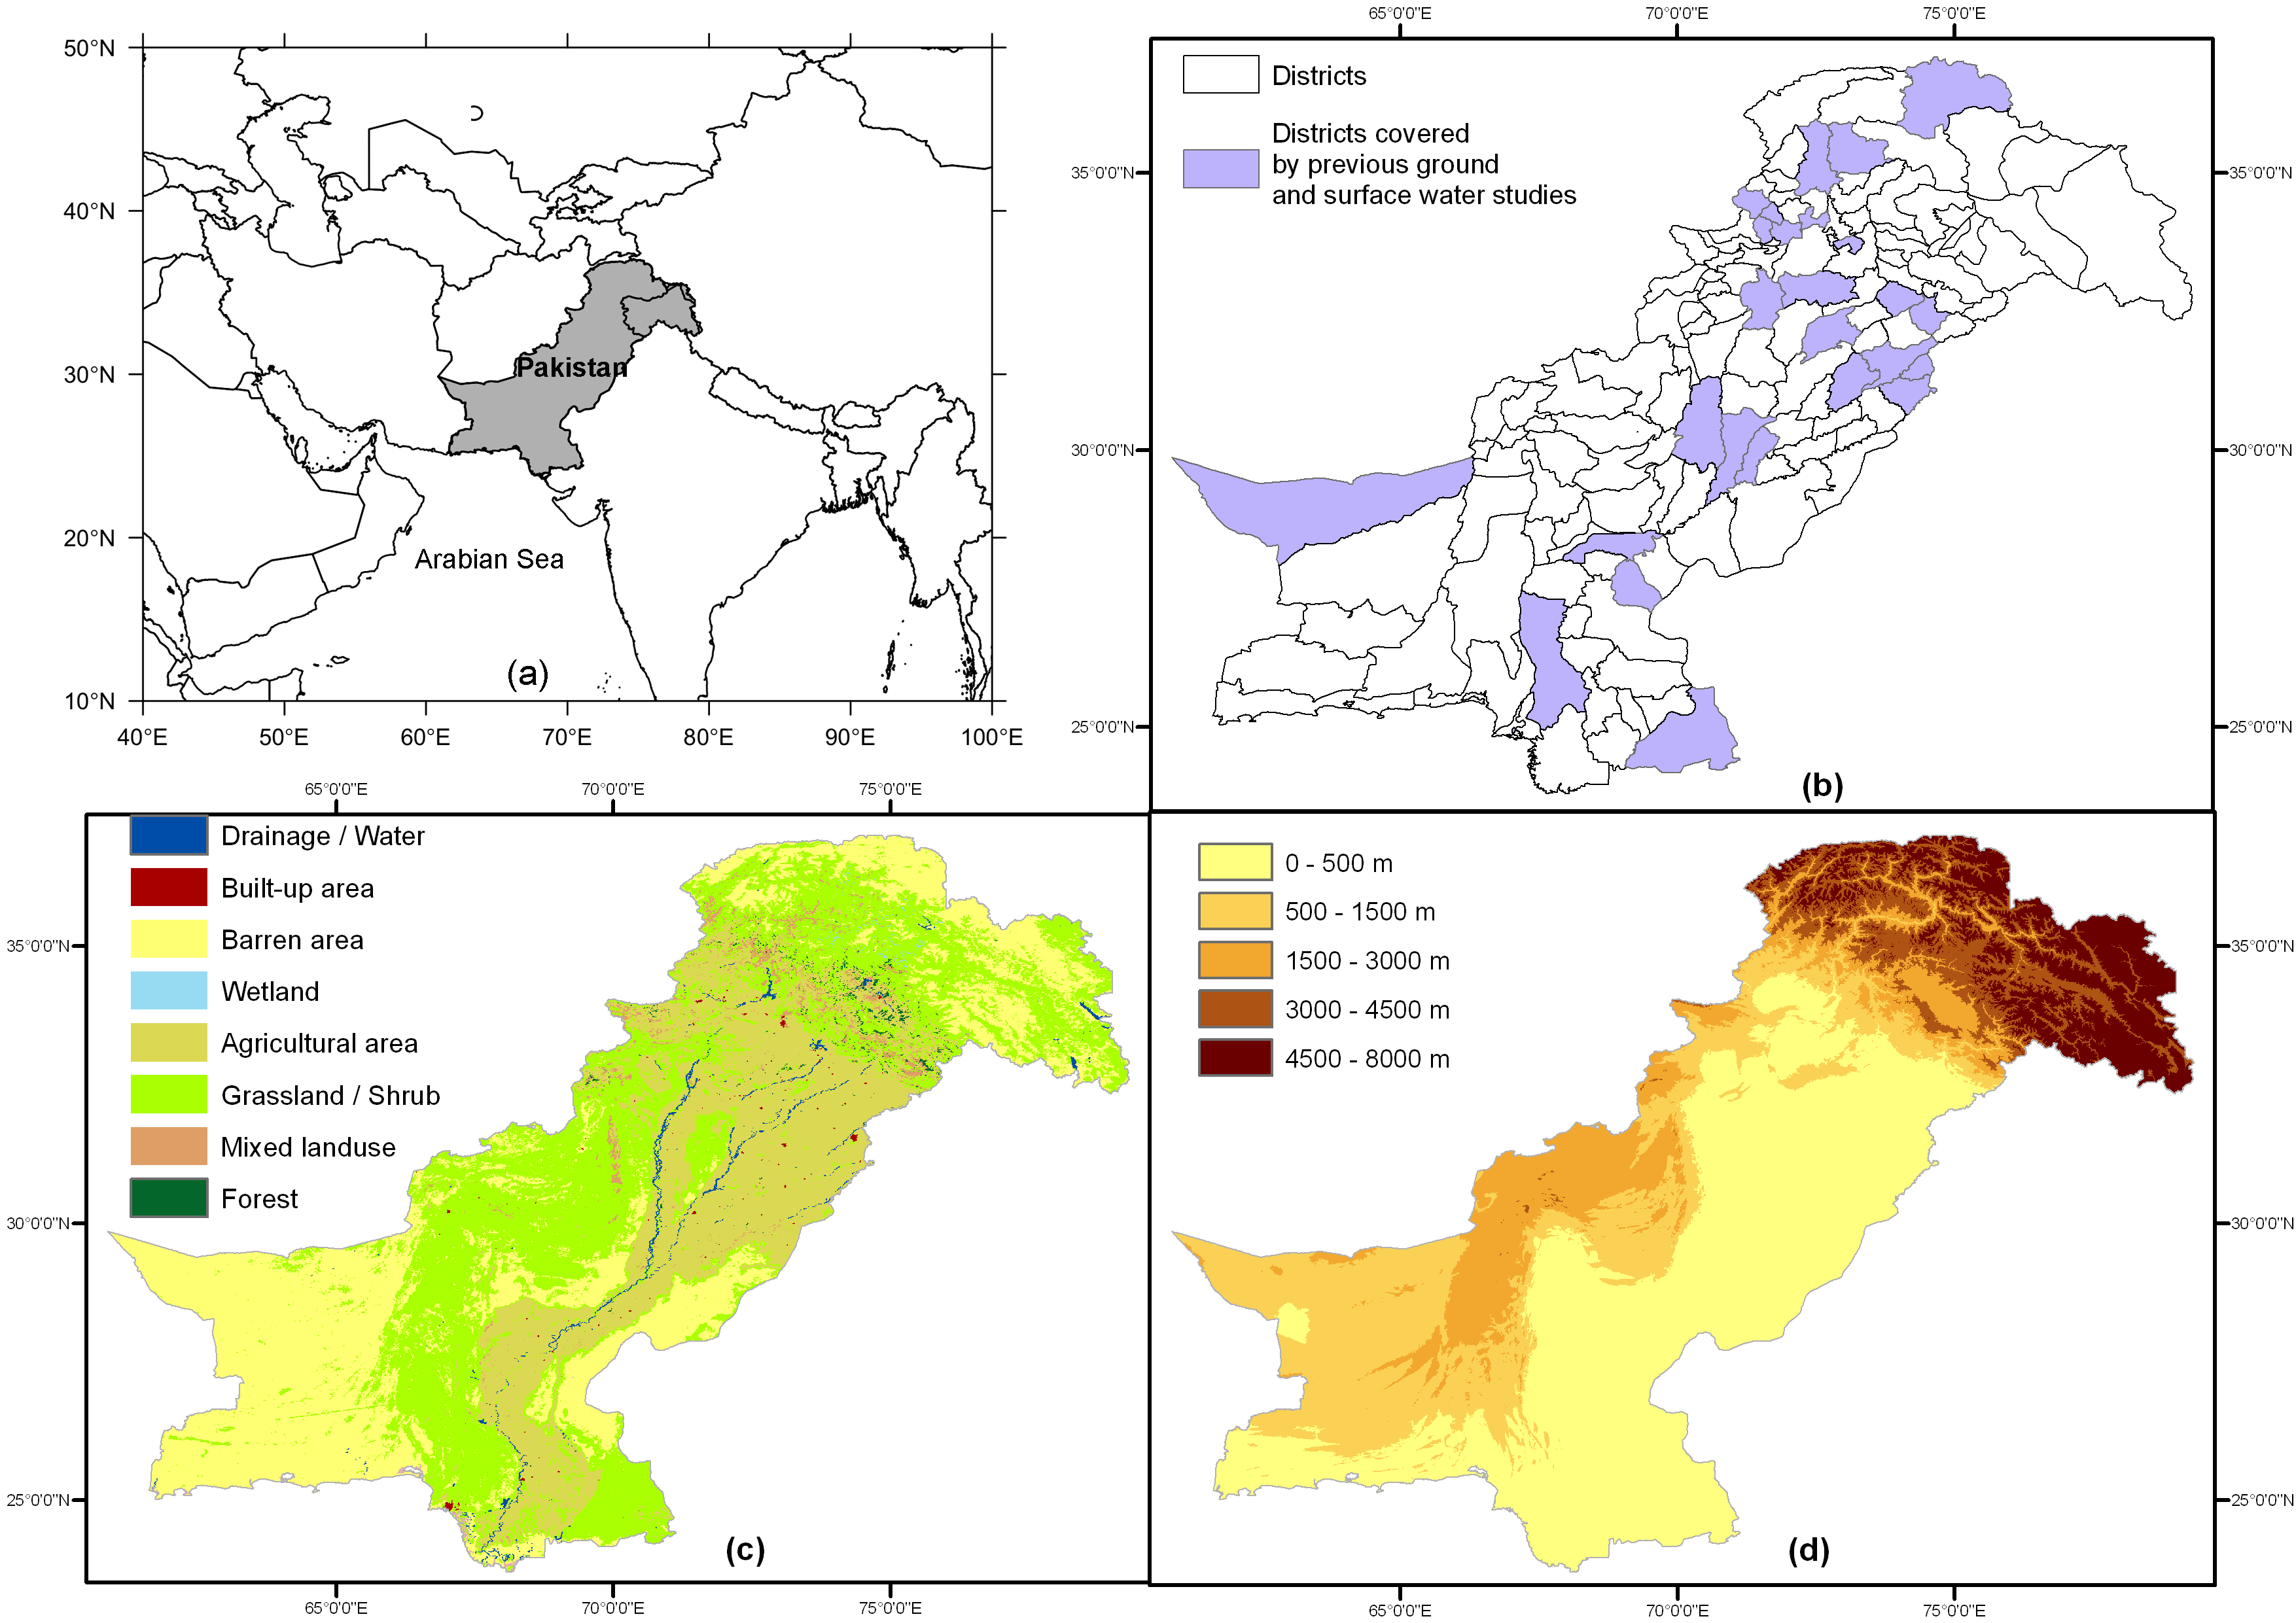
\includegraphics[width=\textwidth]{Figures/Fig_5_1.png}
  \caption{(a) Location of Pakistan in South Asia within the coastal belt of Arabian sea, (b) districts with available trace metal concentration for ground and surface water (see Table D.1 and D.2 in appendix D for details), (c) land cover map of Pakistan with the Indus river basin in the Eastern part of the country (ISCGM, 2014) and (d) elevation of Pakistan from mean sea level (Rodriguez et al., 2005).}
  \label{Fig_5_1}
\end{figure}

\subsection{Data compilation and processing}
\label{Data compilation and processing}

We compiled data on the concentrations of 10 trace metals, i.e. arsenic (As), cadmium (Cd), chromium (Cr), copper (Cu), iron (Fe), manganese (Mn), mercury (Hg), nickel (Ni), lead (Pb) and zinc (Zn) in ground and surface water of Pakistan, measured in multiple sites within 26 districts during 1991-2014, from previously published studies (Table D.1 and D.2 in appendix D). The individual studies provided concentration values that were typically corrected for sampling and processing errors (see cited studies in Table D.1 and D.2). In 82\% of the studies, concentration data were reported as summary statistics (e.g. mean, max and standard deviation, see Table D.1 and D.2 for details on the number of ground and surface water samples in each district used to compute the district mean) for the districts. The trace metal concentrations of samples from each district exhibited a low variation (all coefficient of variation (CV) $\leq$ 20\% and relative homogeneity of CV across districts) and no outlier value was detected in the data (cited studies in Table D.1 and D.2). Hence, given that in 96\% of the studies sampling sites were not geo-referenced, we regarded the mean as a sufficiently robust parameter and assigned district mean values to the georeferenced districts as the representative trace metal concentrations in the surface and ground water (country-level summary statistics are presented in Table D.3). In 5\% and 32\% of districts for ground and surface water, respectively, we had mean concentrations from two years for a few trace metals (Table D.1; D.2). In these cases, we used the latest concentrations to avoid heterogeneity in the uncertainty of predicted concentrations across trace metals and districts, and thus in risk assessment. The district level aggregation of trace metal concentrations may result in uncertainties regarding variability within the districts. However, given the large spatial extent of our study, i.e. country-level with 137 districts, we regarded information on the district-level variation as sufficient. Moreover, previous studies successfully predicted and analyzed the relationship of contaminants, diseases and other variables with their relevant drivers on similar or coarser spatial resolutions, e.g. counties (Videras, 2014), districts (Huang and Leung, 2002), and regions (Berke, 2004).

To identify the deviation in district-level trace metal concentrations from the country-level (global) mean and thus their global representativeness, we computed the global coefficient of variation (GCV) for each trace metal T (Eq. 5.1).

\begin{equation}
GCV_T=\frac{\sigma_T}{\mu_T}+100
\end{equation}

where, $\sigma_T$ and $\mu_T$ are the global standard deviation and mean of the district-level T trace metal concentrations, respectively.

Physical and chemical processes in surface and groundwater and sediment compositions are predominantly affected by adjacent soil properties and further geo-hydrological variables (e.g. soil type, depth of groundwater table, infiltration, seepage and climate), land use (e.g. industrial and agricultural) and different environmental variables (e.g. slope), and in turn these variables show strong correlations with trace metal concentrations (Huang et al., 2015; Pebesma and Kwaadsteniet, 1997; Rodríguez-Lado et al., 2013). Hence, we compiled raster data on the soil properties (also as surrogates of geo-hydrological variables because they are presumably correlated), land cover and elevation (surrogate of environmental variables) for Pakistan. Soil properties data with 0.5 degrees (\textasciitilde 55.5 km) resolution, land cover data with 0.008 degrees (\textasciitilde 925 m) resolution and elevation data with 90 m resolution were obtained from the global soil properties dataset (Batjes, 2000), the Global Map of Pakistan: version 1.1 (ISCGM, 2014) and the digital elevation model (DEM) from Shuttle Radar Topography Mission (SRTM) (Rodriguez et al., 2005), respectively. The data were cropped to the spatial extent of Pakistan and transformed to the WGS 1984 coordinate reference system. The soil properties and land cover data initially included six and eight variables, respectively (Batjes, 2000; ISCGM, 2014). From all raster cells within each district with trace metal concentration data (sampled), the mean soil properties and percentages of different land covers were computed and checked for their spatial correlation with trace metal concentrations. The four soil property variables, i.e. total available water capacity (WC, mm water per 1 m soil depth), soil organic carbon density (SOC, kg C/m\textsuperscript{2} for 0-100 cm depth range), soil carbonates carbon density (SCC, kg C/m\textsuperscript{2} for 0-100 cm depth range) and soil pH (30-100 cm depth range), and the three land cover variables, i.e. \% built-up area (BLU), \% agricultural area (ALU) and \% mixed land use (MLU) area that showed statistically significant correlation with at least one trace metal concentration were included in the final analysis. For these subsetted variables, we extracted the means (for soil property variables) and percentages (for land cover variables) from the rasters also for the districts without trace metal concentrations (unsampled). In addition, the mean elevation (ELV) was calculated per district. Finally, we collected population data for Pakistani districts from the Pakistan Bureau of Statistics (2010). Spatial transformation and extraction of spatial predictor variables was performed using the “maptools” (Lewin-Koh et al., 2011) and “raster” (Hijman and Van Etten, 2010) packages in R (R Core Team, 2014).

\subsection{Spatial prediction of trace metal concentrations in ground and surface water}
\label{Spatial prediction of trace metal concentrations in ground and surface water}

The geographically weighted regression (GWR) model was applied for spatial prediction of the trace metal concentrations in the ground and surface water, separately, at unsampled districts fitted with selected spatial predictors (Fotheringham et al., 2002; Harris et al., 2010). District level trace metal concentrations showed a high dispersion from the global mean (GCV $>$ 1) and hence indicated a low global representativeness (Table D.3). Moreover, only a few districts were sampled by the previous studies resulting in a low sample density and thus large distances between the districts (Figure 5.1; Table D.3). Hence, the GWR model was chosen because it allows to incorporate local variations of the trace metal concentrations with respect to spatial auto-correlation and non-stationarity in the model parameters (Fotheringham et al., 2002; Harris et al., 2010). Moreover, compared to global spatial prediction techniques such as kriging, the GWR has been shown to better represent the spatially varying relationship between water quality parameters and different spatial predictors (Javi et al., 2014; Huang et al., 2015; Tu and Xia, 2008). Furthermore, GWR allowed for modelling spatial variability of trace metals at district level resolution with low uncertainty (Lin et al., 2011). A GWR model was calibrated for the concentration of each trace metal $T$ in ground and surface water for the sampled districts $z$ by evaluating the local relationship between trace metal concentration $C_{T,z}$ and spatial predictors $S$ (Eq. 5.2).

\begin{equation}
C_{T,z}=\delta_{z,0}+\displaystyle\sum_{n=1}^{m=8}\delta_{z,n}S_{z,n}+e_z
\end{equation}

where $S_{z,n}$ is the value of the $n$th spatial predictor (={WC, SOC, SCC, pH, BLU, ALU, MLU and ELV}), $m$ is the number of spatial predictors (=8), $\delta_{z,0}$ is the intercept parameter, $\delta_{z,n}$ is the local regression coefficient for the $n$th spatial predictor and $e_z$ is the random error. The GWR model estimates the local regression coefficients for the spatial predictors using a moving window technique and a weighted least square approach (Figure D.1). The weights are obtained using a distance-decay kernel function among the centroids of neighboring sampled districts. We chose a “gaussian” kernel, based on the assumption of spatial continuity of the trace metal concentration in ground and surface water, as the water bodies are connected through a network within the Indus river delta (Harris et al., 2010; Pakistan Bureau of Statistics, 2010). The size of the moving window (great circle distances between district centroids in our case) is controlled by a kernel bandwidth that was selected using the Akaike Information Criterion corrected for small sample sizes (AICc) (Table 5.1) (Akaike, 1973). For each trace metal, the best-fit GWR model was identified by forward entering of the eight spatial predictors and using the AICc values as goodness of fit criterion. The best-fit model (minimal AICc) was selected for prediction of each of the trace metals in ground and surface water, separately, in unsampled districts (Figure 5.2; 5.3). Spatial prediction for Hg in ground water was omitted because of the very small sample size (n= 2) (Table D.3). GWR model selection, calibration and the spatial prediction were performed using the “GWmodel” package (Gollini et al., 2013) in R (R Core Team, 2014).

\subsection{GWR model validation}
\label{GWR model validation}

We evaluated the spatial prediction quality of the GWR models in terms of prediction accuracy and the agreement between model predicted and observed concentrations (Gollini et al., 2013). To predict the accuracy, the observed concentrations of a district were compared to the concentrations

\begin{landscape}

\begin{table}[h]

\label{Table 5.1}

\caption{Calibrated geographically weighted regression (GWR) models and their spatial prediction quality for the concentration of trace metals in ground and surface water of unsampled districts. Corresponding corrected Akaike Information Criterion (AICc), kernel bandwith (size of the moving window), root mean square deviation error (RMSDE), index of agreement ($d$), mean (MZ) and standard deviation (SDZ) of the prediction z-scores are provided.}

\begin{threeparttable}
\centering

\begin{tabular}{>{\centering\arraybackslash}m{2.0cm}>{\centering\arraybackslash}m{2.0cm}>{\centering\arraybackslash}m{3.0cm}>{\centering\arraybackslash}m{1.5cm}>{\centering\arraybackslash}m{4.0cm}>{\centering\arraybackslash}m{0.7cm}>{\centering\arraybackslash}m{0.7cm}>{\centering\arraybackslash}m{1.0cm}>{\centering\arraybackslash}m{0.7cm}}

\toprule
\multirow{2}{2.0cm}{\centering\textbf{Trace metal}} & \multirow{2}{2.0cm}{\centering\textbf{Source}} & \multirow{2}{3.0cm}{\centering\textbf{Selected GWR model}} & \multirow{2}{1.5cm}{\centering\textbf{AICc}} & \multirow{2}{4.0cm}{\centering\textbf{Kernel bandwith (great circle distance between district centroids, km)}} & \multicolumn{2}{c}{\centering\textbf{Prediction quality}} & \multicolumn{2}{c}{\centering\textbf{Prediction uncertainty}}\\
 & & & & & \textbf{RMSDE} & \textbf{$d$} & \textbf{MZ} & \textbf{SDZ}\\
 & & & & & & & & \\

\midrule

\multirow{2}{2.0cm}{\centering As} & Ground water & As\textunderscore GW \textasciitilde SOC & 13.46 & 1104.30 & 0.27 & 0.67 & -0.01 & 0.77\\
 & Surface water & As\textunderscore SW \textasciitilde SOC+pH & -1255.80 & 521.98 & 0.08 & 0.97 & -0.06 & 0.22\\
\multirow{2}{2.0cm}{\centering Cd} & Ground water & Cd\textunderscore GW\textasciitilde SOC+SCC & -9140.39 & 1299.72 & 0.06 & 0.90 & -0.10 & 0.13\\
 & Surface water & Cd\textunderscore SW\textasciitilde ALU & -29.10 & 1321.05 & 0.04 & 0.79 & -0.01 & 0.69\\
\multirow{2}{2.0cm}{\centering Cr} & Ground water & Cr\textunderscore GW\textasciitilde BLU & -21.27 & 500.64 & 0.06 & 0.99 & 0.00 & 0.77\\
 & Surface water & Cr\textunderscore SW\textasciitilde WC+ALU & -4014.42 & 1321.14 & 0.04 & 0.92 & -0.05 & 0.21\\
\multirow{2}{2.0cm}{\centering Cu} & Ground water & Cu\textunderscore GW\textasciitilde SOC & 33.75 & 1299.58 & 0.61 & 0.43 & 0.00 & 0.75\\
 & Surface water & Cu\textunderscore SW\textasciitilde WC & -31.45 & 1321.05 & 0.04 & 0.79 & -0.03 & 0.74\\
\multirow{2}{2.0cm}{\centering Fe} & Ground water & Fe\textunderscore GW\textasciitilde WC & 43.33 & 1147.75 & 0.97 & 0.39 & 0.02 & 0.77\\
 & Surface water & Fe\textunderscore SW\textasciitilde SOC & 45.45 & 1320.77 & 0.95 & 0.44 & 0.00 & 0.78\\
\multirow{2}{2.0cm}{\centering Mn} & Ground water & Mn\textunderscore GW\textasciitilde SCC+BLU & -9764.11 & 1299.72 & 0.22 & 0.95 & -0.06 & 0.14\\
 & Surface water & Mn\textunderscore SW\textasciitilde WC+ALU & -3675.37 & 1321.14 & 0.07 & 0.86 & -0.05 & 0.20\\
Hg & Surface water & Hg\textunderscore SW\textasciitilde SCC+BLU & -1543.69 & 453.07 & 0.02 & 0.98 & -0.06 & 0.30\\
\multirow{2}{2.0cm}{\centering Ni} & Ground water & Ni\textunderscore GW\textasciitilde SCC & 22.88 & 1299.36 & 0.42 & 0.51 & -0.03 & 0.78\\
 & Surface water & Ni\textunderscore SW\textasciitilde WC & -29.23 & 1335.07 & 0.04 & 0.88 & -0.02 & 0.70\\
\multirow{2}{2.0cm}{\centering Pb} & Ground water & Pb\textunderscore GW\textasciitilde BLU & 8.52 & 1299.49 & 0.21 & 0.96 & -0.02 & 0.78\\
 & Surface water & Pb\textunderscore SW\textasciitilde ALU & -18.70 & 1321.00 & 0.07 & 0.75 & 0.01 & 0.75\\
\multirow{2}{2.0cm}{\centering Zn} & Ground water & Zn\textunderscore GW\textasciitilde BLU & 26.64 & 1299.36 & 0.45 & 0.95 & 0.01 & 0.80\\
 & Surface water & Zn\textunderscore SW\textasciitilde SOC & 42.63 & 1335.07 & 0.80 & 0.31 & -0.01 & 0.79\\

\bottomrule

\end{tabular}

\begin{tablenotes}
\footnotesize
As = Arsenic, Cd = Cadmium, Cr = Chromium, Cu = Copper, Fe = Iron, Mn = Manganese, Hg = Mercury, Nickel = Ni, Pb = Lead, Zn = Zinc,  GW = ground water, SW = surface water, WC = mean total available water capacity, SOC = mean soil organic carbon density, SCC = mean soil carbonate carbon density, pH= mean soil pH, BLU = percentage of built-up area, ALU = percentage of agricultural area.
\end{tablenotes}

\end{threeparttable}

\end{table}

\end{landscape}

\noindent predicted for this district using the respective GWR model in terms of root mean squared deviation error (RMSDE) (Eq. 5.3) computed through a leave-one-out cross validation (see Gollini et al. (2013) for details). Similarly, the index of agreement ($d$) was computed to quantify the agreement between GWR model predicted and observed trace metal ($T$) concentrations (Eq. 5.4) (Table 5.1) (Willmott, 1984).

\begin{equation}
RMSDE_T=\displaystyle\sum_{z=1}^{n}\sqrt{\frac{1}{n}(P_{T,z}-O_{T,z})^2}
\end{equation}

\begin{equation}
d_T=1-\frac{n*RMSDE_T^2}{\displaystyle\sum_{z=1}^{n}(|P_{T,z}-\bar{O}_T|+|O_{T,z}-\bar{O}_T|)^2}
\end{equation}

where, $RMSDE_T$ and $d_T$ are the RMSDE and $d$ for the GWR model predictions, $P_{T,z}$ and $O_{T,z}$ are model predicted and observed concentration values in district $z$, $n$ is the number of districts and $\bar{O}_T$ is the mean of the observed district level concentrations. The RMSDE should tend to zero to indicate the accurate prediction of GWR. The $d$ values vary on a scale from 0 to 1, 0 indicating no agreement and 1 the perfect agreement. GWR model validation was performed using the “GWmodel” (Gollini et al., 2013) and “hydroGOF” (Zambrano-Bigiarini, 2014) packages in R (R Core Team, 2014).

\subsection{GWR prediction uncertainties}
\label{GWR prediction uncertainties}

We computed nationwide (global) GWR prediction uncertainties for trace metal concentrations in ground and surface water by the mean (MZ) standard deviation (SDZ) of the prediction z-scores (Table 5.1) (Gollini et al., 2013).  Zero MZ and the unity of SDZ indicate high certainty in the prediction by GWR. In a second step, we calculated standard error maps for predictions of trace metal concentrations in ground and surface water to investigate the GWR model prediction uncertainties for each district (local) (Figure D.2). Finally, we computed ranges in the GWR model predicted trace metal concentration values within 95\% confidence interval based on local prediction uncertainties, i.e. GWR predicted values $\pm$ 1.96 * standard errors (Figure D.3; D.4). GWR prediction uncertainty was computed using the “GWmodel” package (Gollini et al., 2013) in R (R Core Team, 2014).

\subsection{Risk prediction}
\label{Risk prediction}

We computed a human health risk quotient (RQ) for each trace metal concentration to predict their exceedances of threshold concentrations in each district (Törnqvist et al., 2011) (Eq. 5.5).

\begin{equation}
RQ_{T,z}=\frac{\hat{C}_{T,z}}{C_{WHO-T}}
\end{equation}

where, for the $T$th trace metal in ground or surface water at district $z$, $\hat{C}_{T,z}$ is the estimated concentration by GWR and $C_{WHO-T}$ is the threshold concentration derived by the World Health Organization (WHO guideline values based on human health targets) for drinking water for the trace metal T (WHO, 2011). In the absence of WHO values for Fe, we used the criteria guidelines values from the environmental protection agency (EPA)-Pakistan (Azizullah et al., 2011). A RQ $\leq$ 1 indicates negligible risk (lower- than or equal concentration to the WHO guideline value), whereas RQ $>$ 1 indicates a health risk (higher concentration than the WHO guideline value) to the consumers from drinking contaminated water (Törnqvist et al., 2011) and, accordingly, the risk related to ground and surface waters for a district was mapped (Figure 5.4; 5.5). Finally, the proportion of total area of Pakistan at risk and total inhabitants in risky districts were calculated through a spatial overlay of the created risk maps with district area and population data (Table 5.2).

\subsection{Risk prediction uncertainties}
\label{Risk prediction uncertainties}

To address the uncertainties in risk prediction, we computed RQ values for the lower and upper confidence boundaries (CB) of predicted trace metal concentrations, i.e. GWR predicted values $\pm$ 1.96 * standard errors (Figure D.5; D.6). The proportion of total area at risk and total inhabitants in risky districts were also computed for the lower and upper CB of predicted trace metal concentrations (Table 5.2).

\begin{figure}[t]
  \centering
  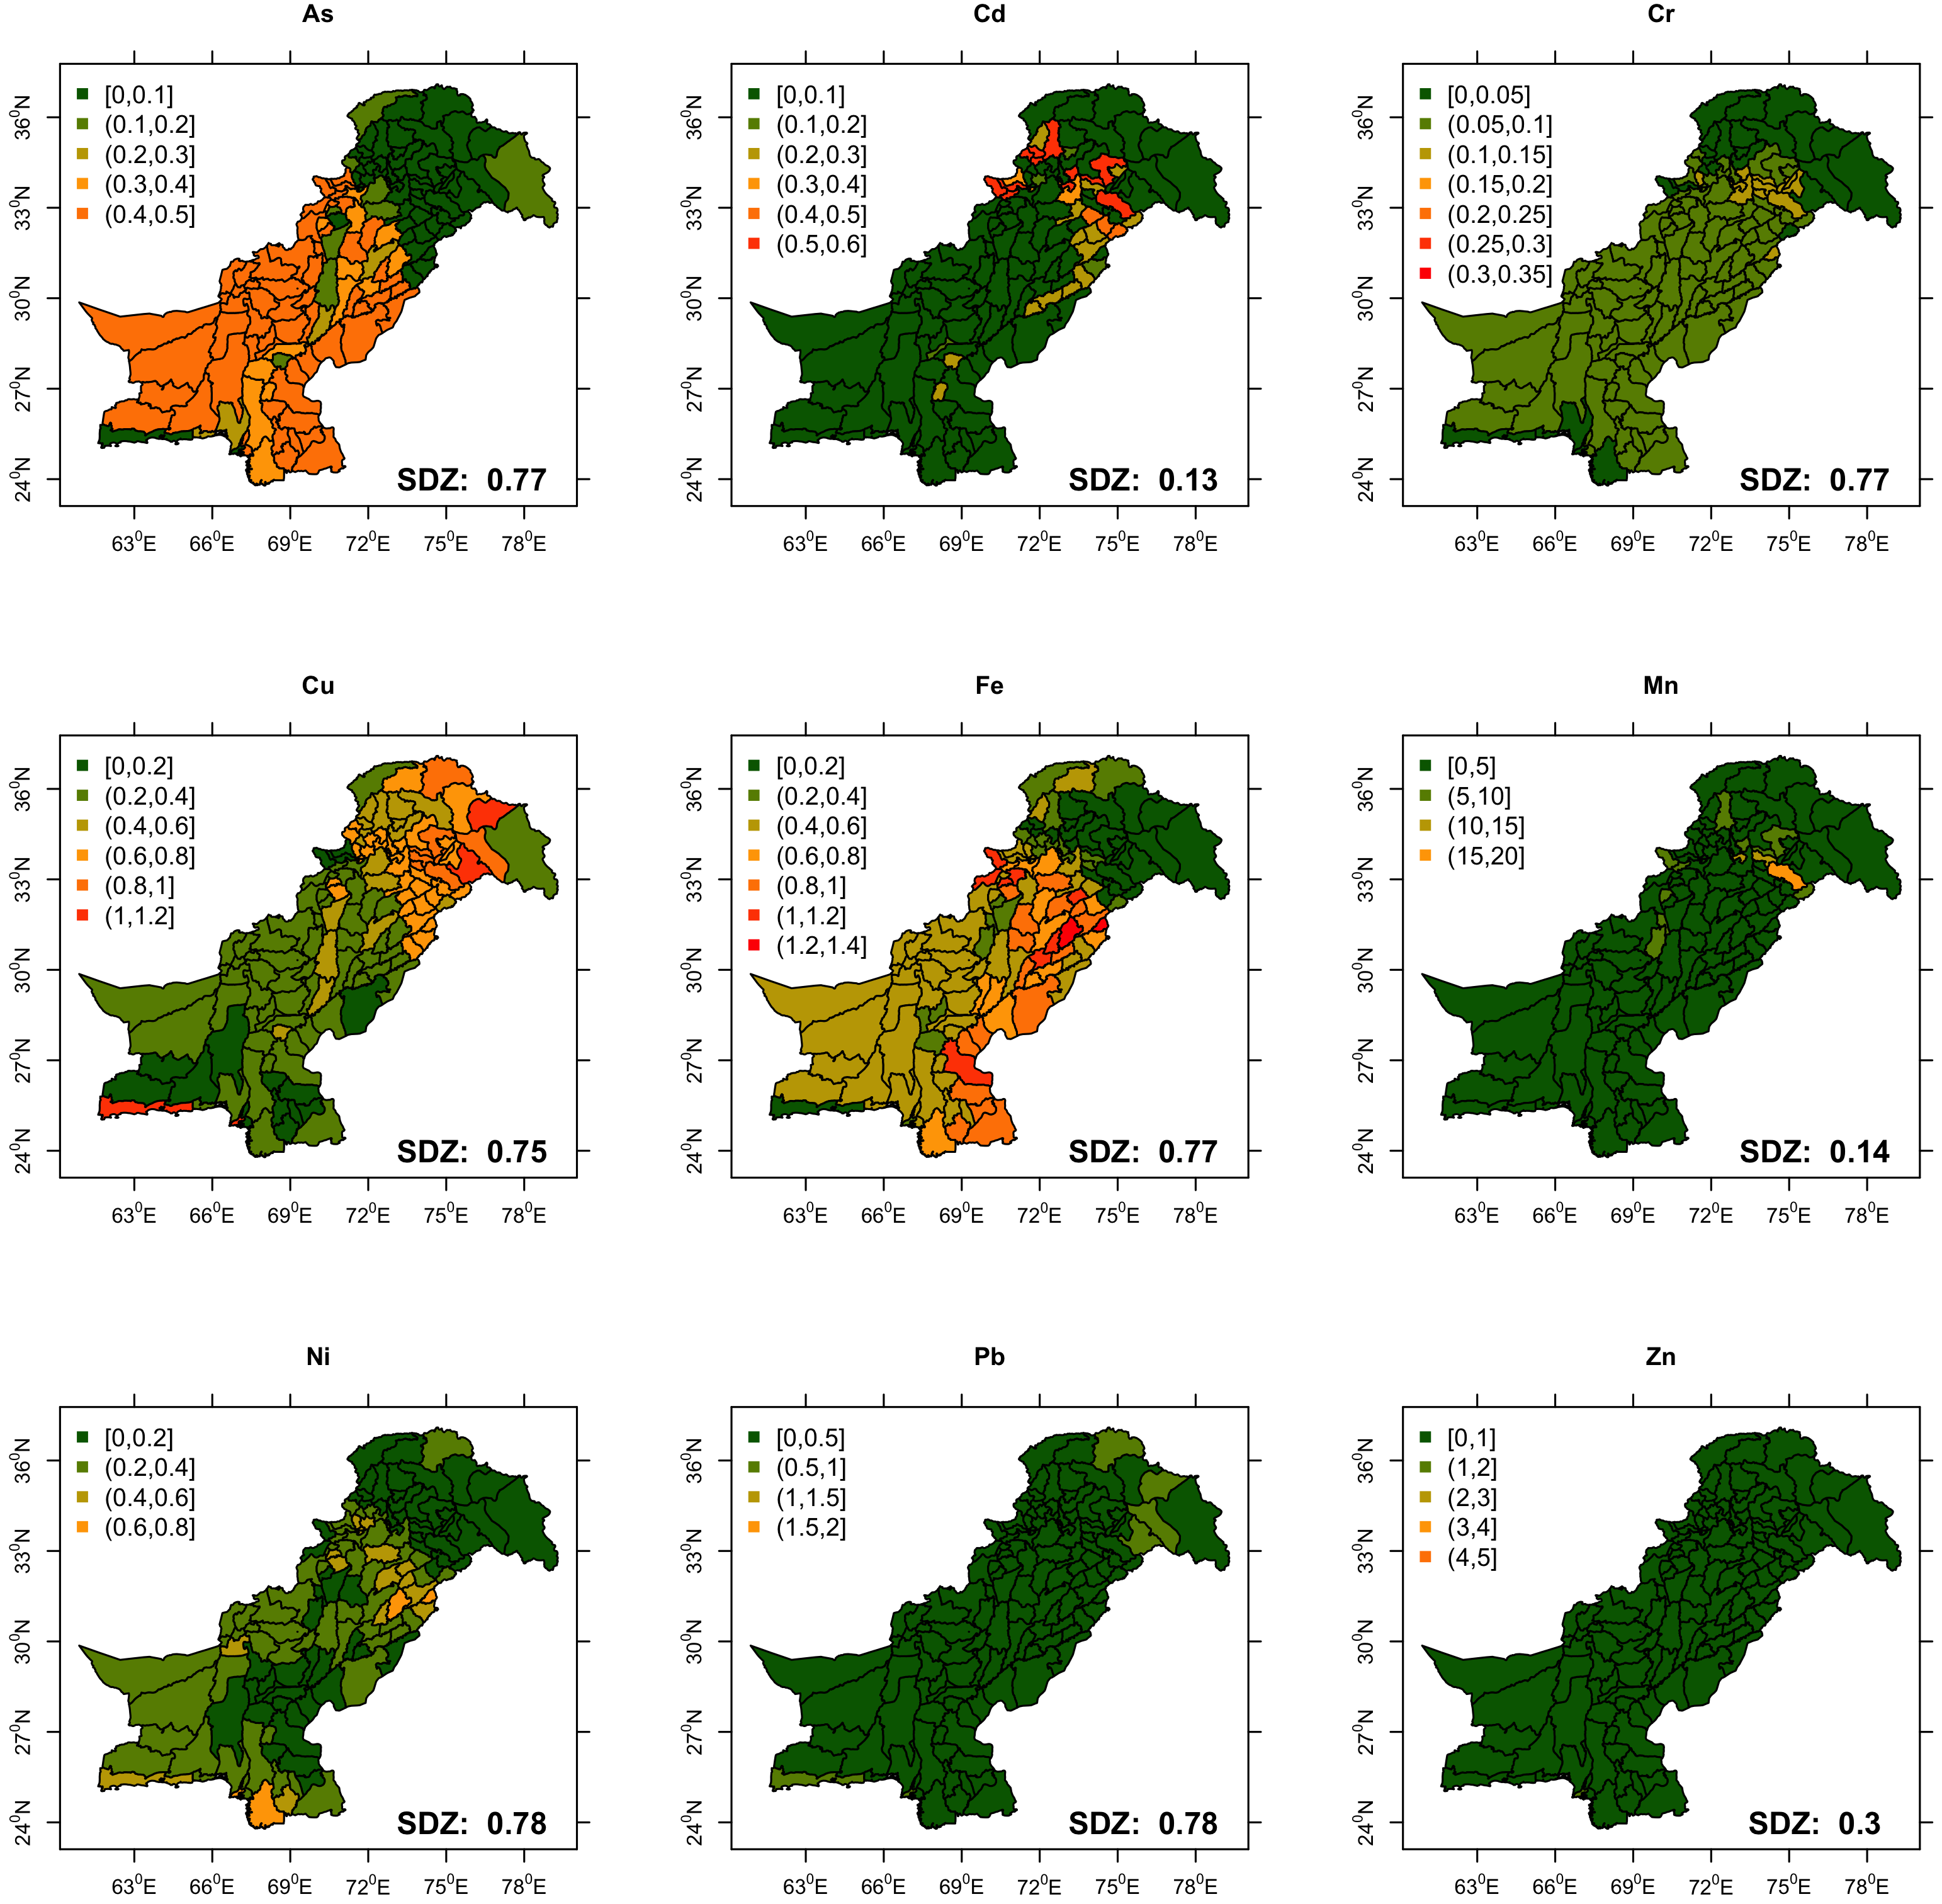
\includegraphics[width=\textwidth]{Figures/Fig_5_2.png}
  \caption{Geographically weighted regression predicted concentration values in mg/l (see legend) of the trace metals in ground water at the districts of Pakistan.  The abbreviations used: As = Arsenic, Cd = Cadmium, Cr = Chromium, Cu = Copper, Fe = Iron, Mn = Manganese, Nickel = Ni, Pb = Lead, Zn = Zinc.}
  \label{Fig_5_2}
\end{figure}

\begin{landscape}
\begin{figure}[t]
  \centering
  \vspace*{-1.5cm}
  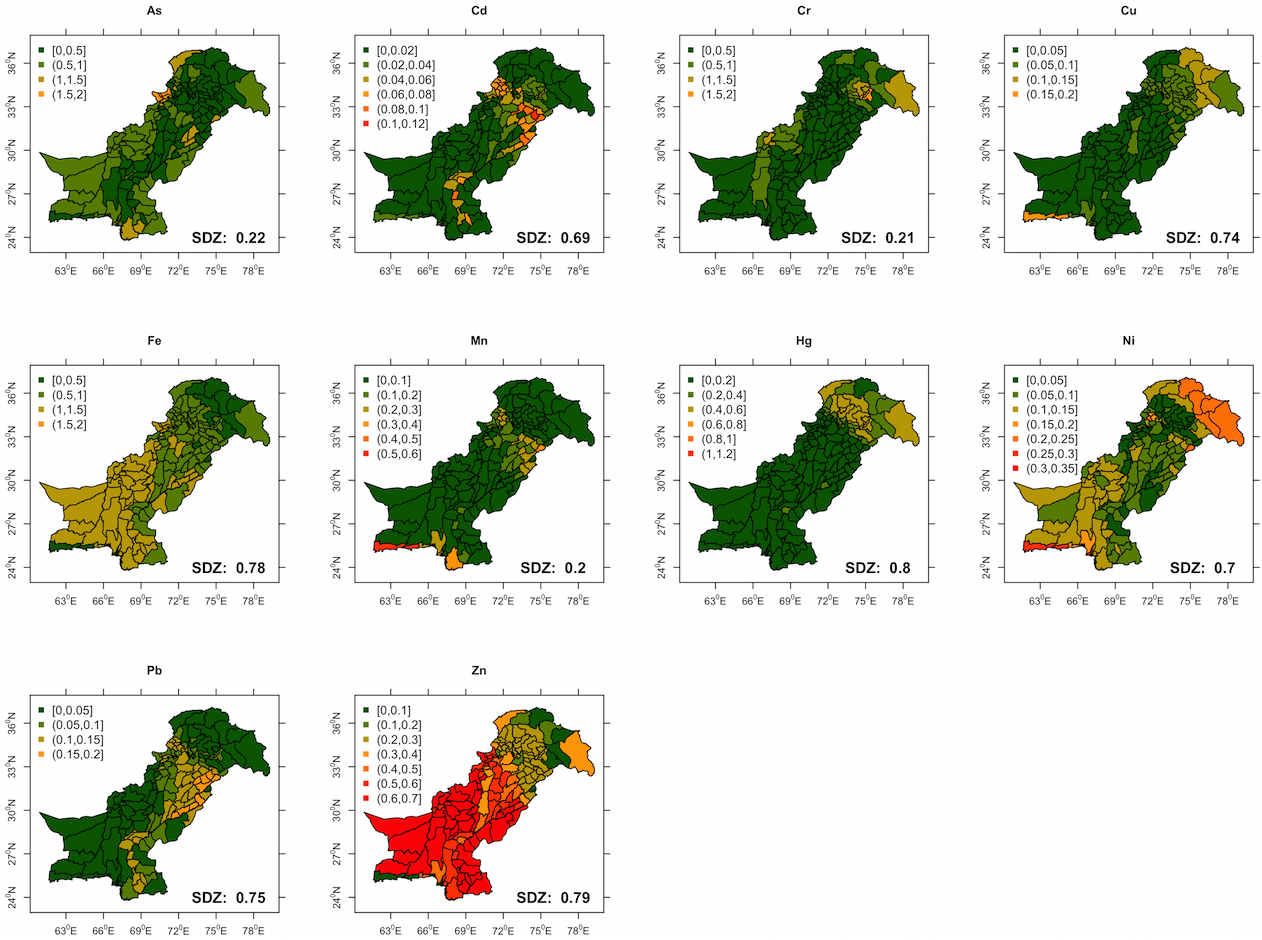
\includegraphics[width=0.9\linewidth]{Figures/Fig_5_3.png}
  \caption{Geographically weighted regression predicted concentration values values in mg/l (see legend) of the trace metals in surface water at the districts of Pakistan.  The abbreviations used: As = Arsenic, Cd = Cadmium, Cr = Chromium, Cu = Copper, Fe = Iron, Mn = Manganese, Hg = Mercury, Nickel = Ni, Pb = Lead, Zn = Zinc.}
  \label{Fig_5_3}
\end{figure}
\end{landscape}

\begin{figure}[t]
  \centering
  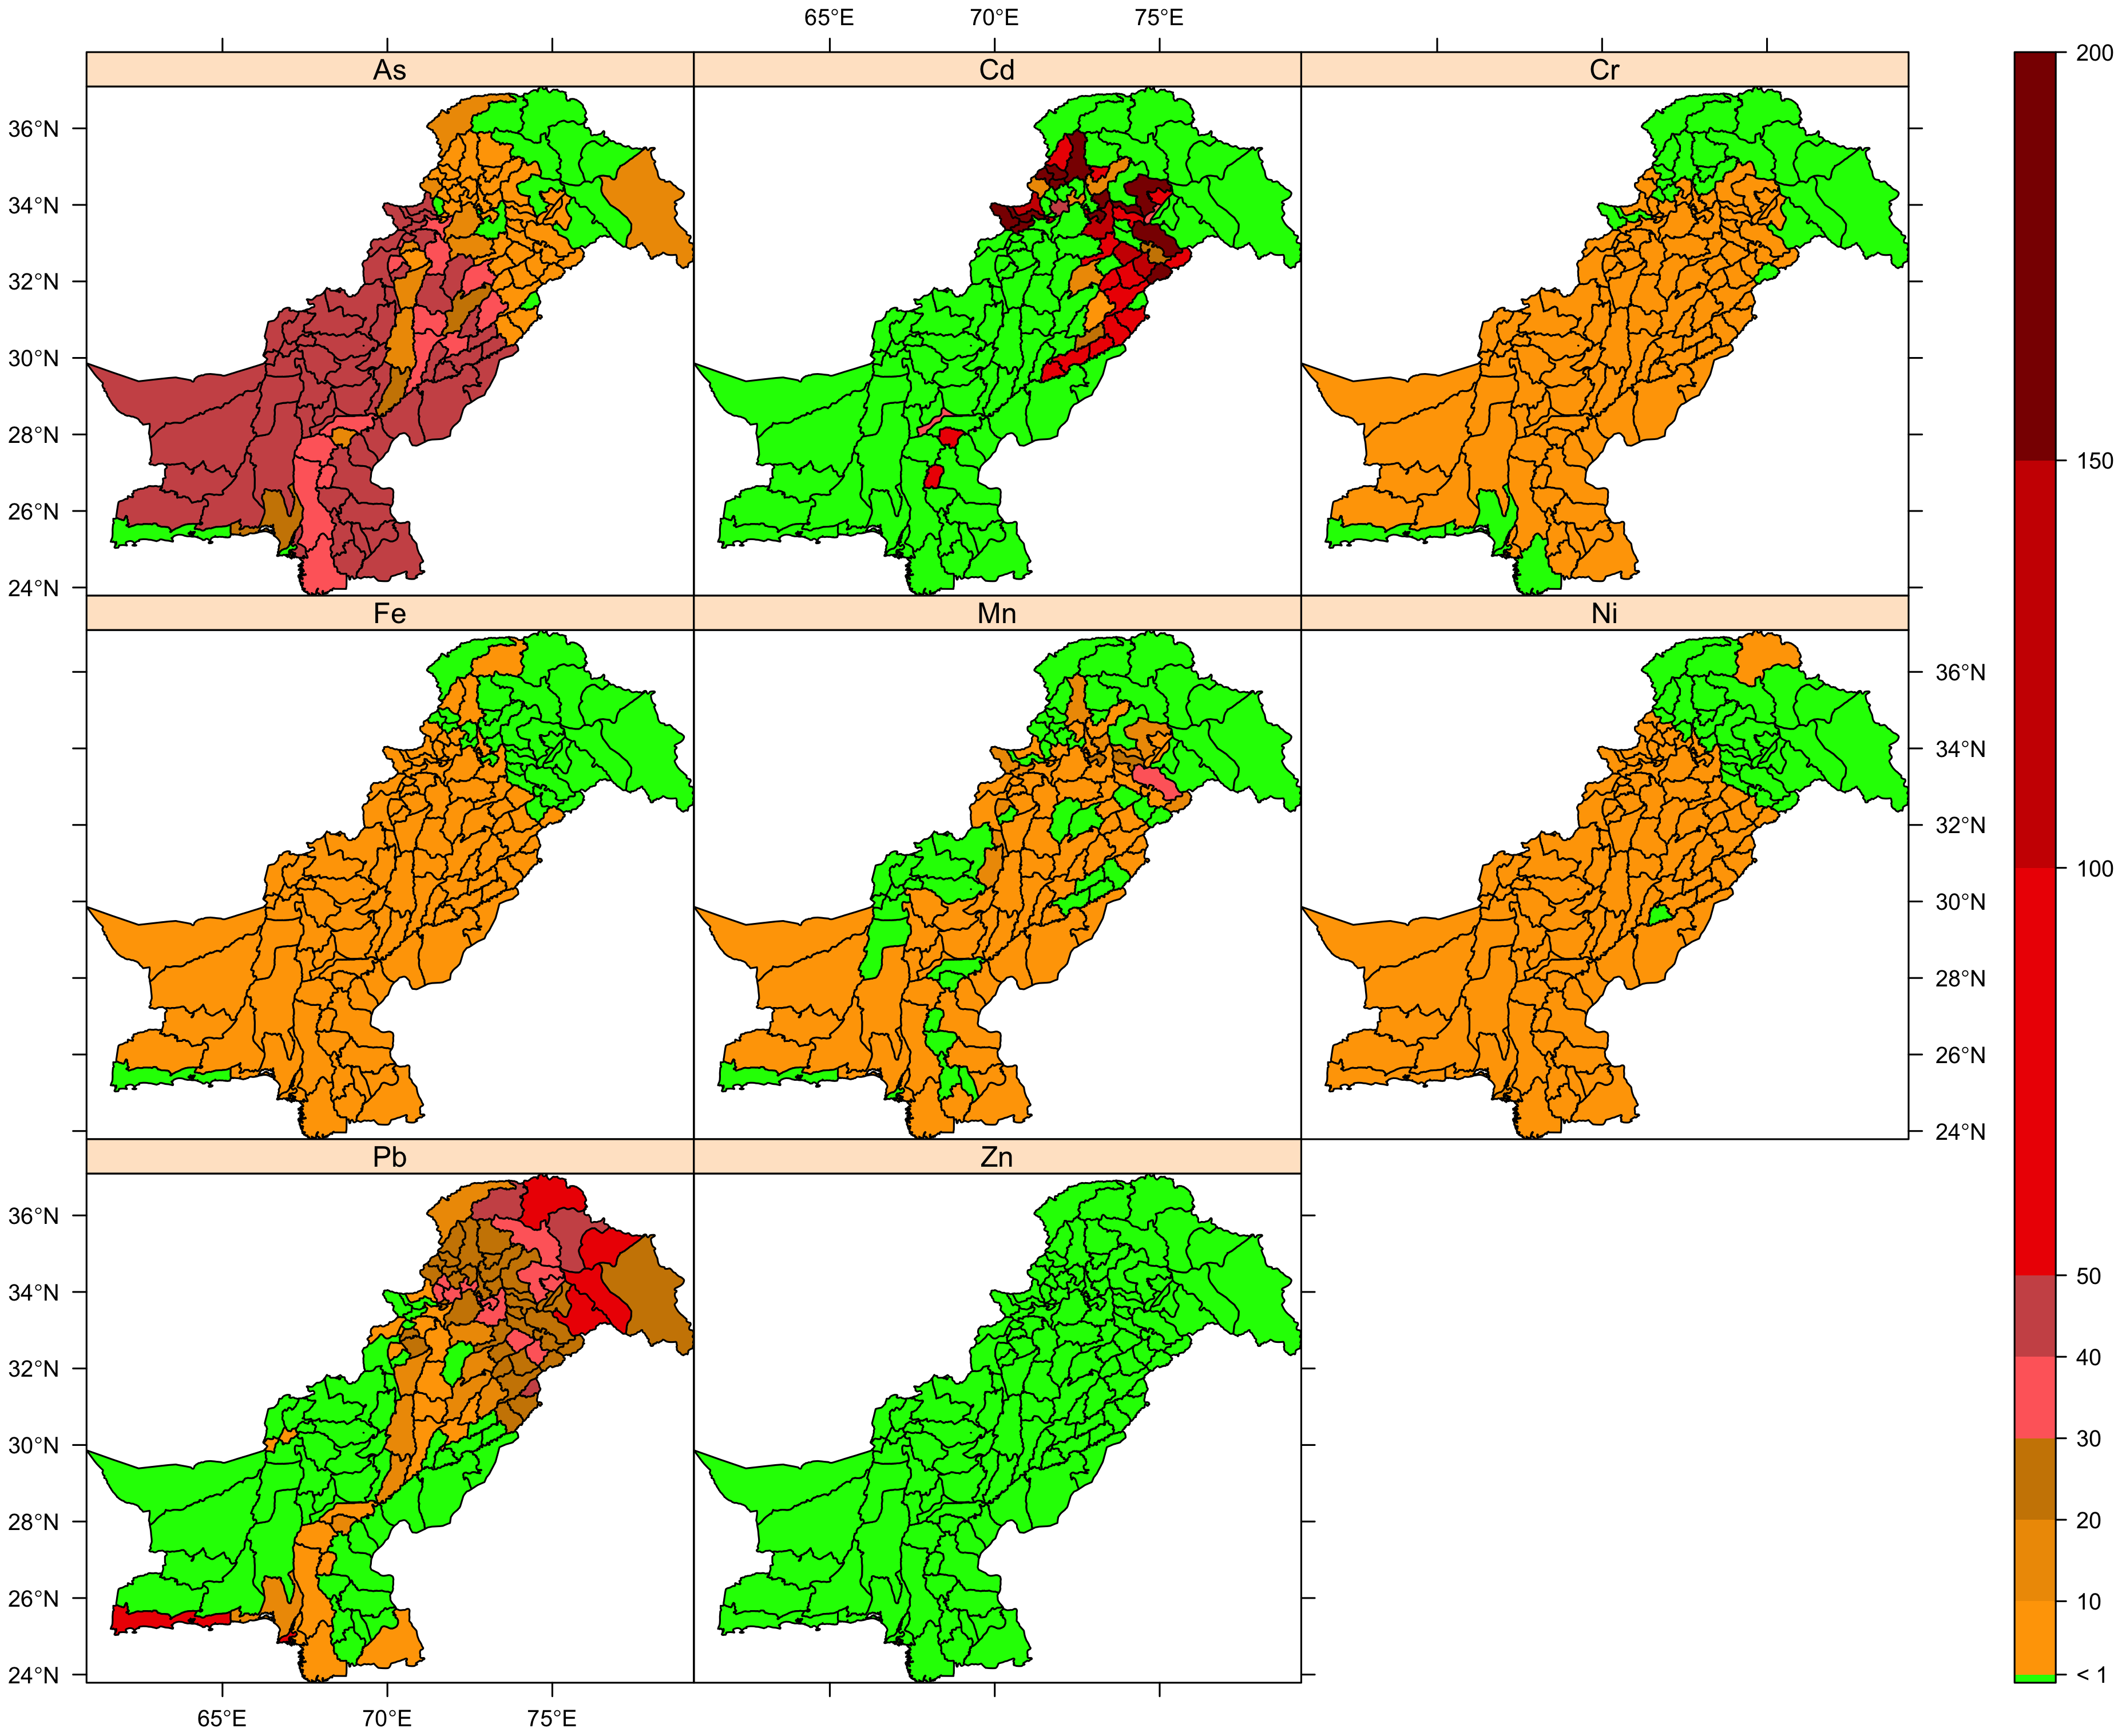
\includegraphics[width=\textwidth]{Figures/Fig_5_4.png}
  \caption{Predicted risks, i.e. exceedances of threshold concentrations in risk quotients (RQ), for the districts of Pakistan from predicted concentrations of trace metals in the ground water. Green indicates no exceedance, i.e. RQ $\leq$ 1. The abbreviations used: As = Arsenic, Cd = Cadmium, Cr = Chromium, Cu = Copper, Fe = Iron, Mn = Manganese, Nickel = Ni, Pb = Lead, Zn = Zinc. Map of Cu is omitted because no risky district was found, i.e. for none of the district RQ $>$ 1.}
  \label{Fig_5_4}
\end{figure}

\begin{figure}[t]
  \centering
  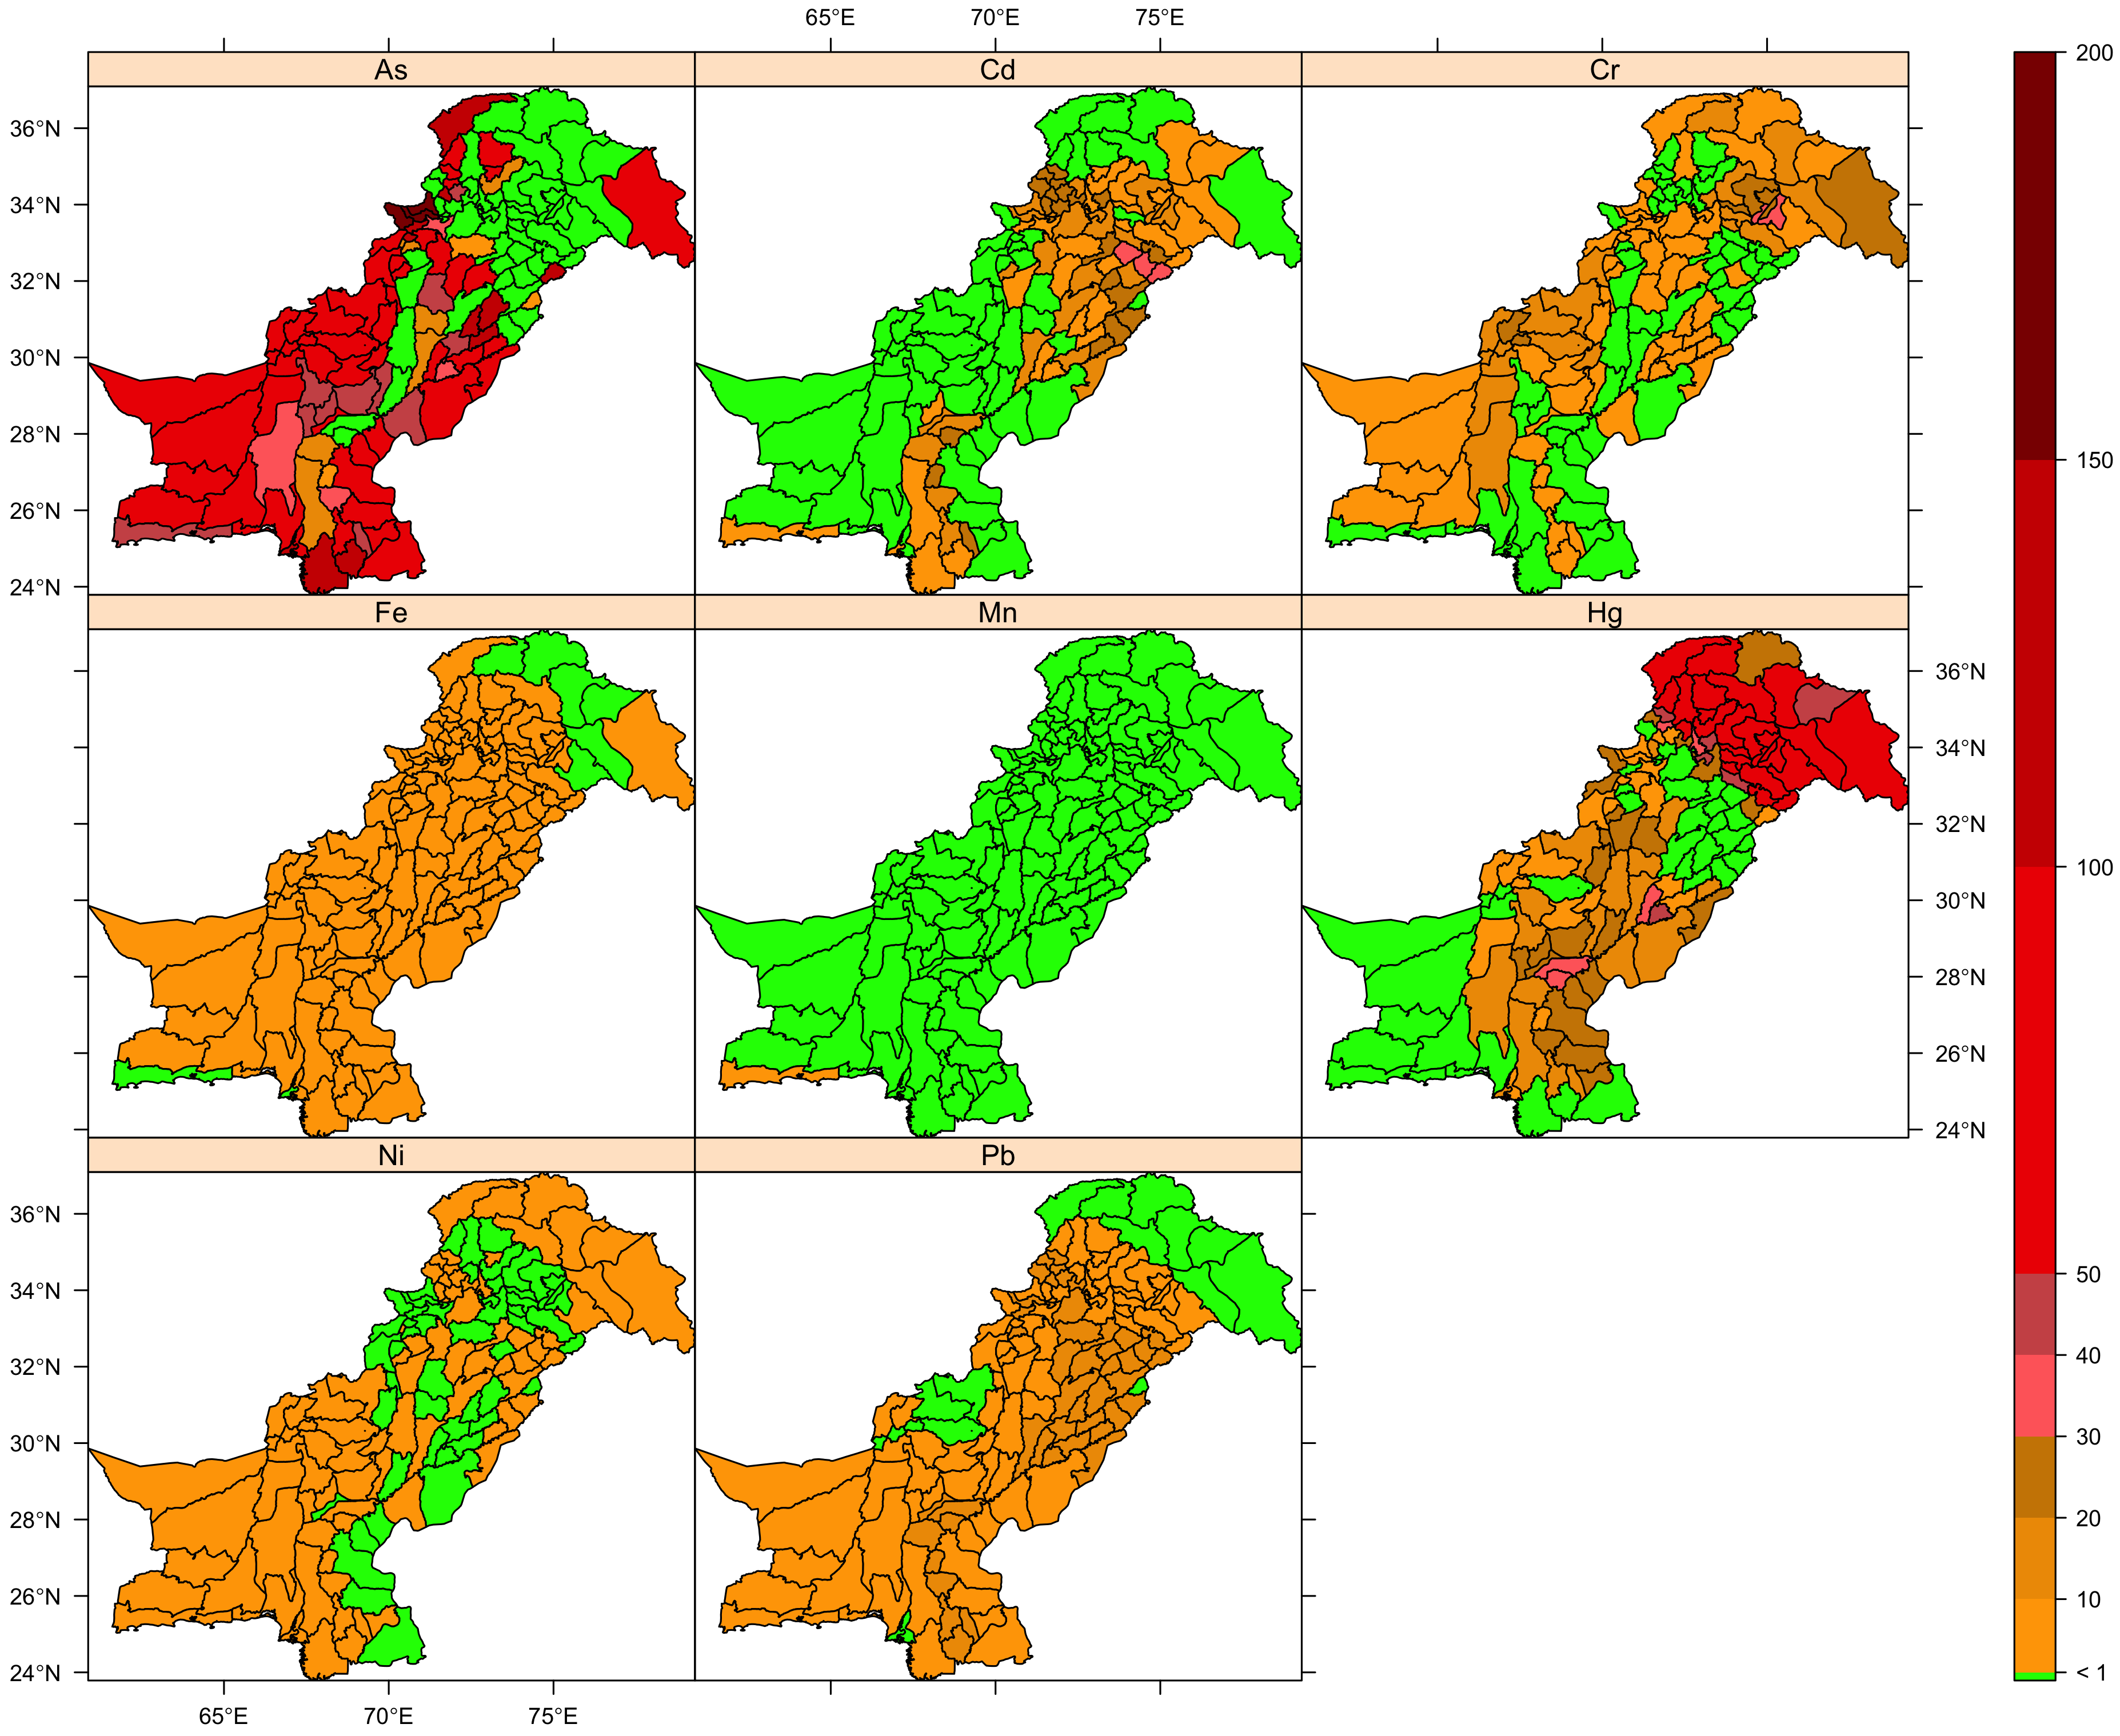
\includegraphics[width=\textwidth]{Figures/Fig_5_5.png}
  \caption{Predicted risks, i.e. exceedances of threshold concentrations in risk quotients (RQ), for the districts of Pakistan from predicted concentrations of trace metals in the surface water. Green indicates no exceedance, i.e. RQ $\leq$ 1. The abbreviations used: As = Arsenic, Cd = Cadmium, Cr = Chromium, Cu = Copper, Fe = Iron, Mn = Manganese, Hg = Mercury, Nickel = Ni, Pb = Lead, Zn = Zinc. Maps of Cu and Zn are omitted because no risky district was found, i.e. for none of the district RQ $>$ 1.}
  \label{Fig_5_5}
\end{figure}

\section{Results and Discussion}
\label{Results and Discussion}

\subsection{GWR prediction of trace metal concentration in ground and surface water}
\label{GWR prediction of trace metal concentration in ground and surface water}

We predicted the concentrations of 10 trace metals in surface and ground water of Pakistan by using the best-fit GWR models with selected spatial predictors. Out of eight spatial predictors that were selected based on statistically significant correlations in a preliminary analysis, six predictors were included in the best-fit GWR models based on the AICc (Table 5.1). Soil properties variables, i.e. WC, SOC, SCC, and pH, which represent a surrogate of geo-hydrological variables, were the spatial predictors of As, Fe and Ni. The As, Fe and Ni contamination of drinking water sources in Pakistan can largely be attributed to the natural geogenic sources that are causally related to the soil properties and geo-hydrology (Azizullah et al., 2011; Shah et al., 2012). For example, As contamination of ground water in many parts of Pakistan results from the presence of Holocene sediments brought by alluvial deposits into arid to semi-arid zones and the subsequent As release due to As-desorption in oxic aquifers (Amini et al., 2008; Farooqi et al., 2008). Moreover, the ground as well as surface water sediments are rich in “micas” dominated by “biotite” mineral that contains As and releases As under high pH level (Husain et al., 2012). Furthermore, surface water from the Himalayas erodes As-rich sediments resulting in elevated As levels in downstream areas (Husain et al., 2012). By contrast, agricultural (ALU) and built-up (BLU) land covers were the dominant predictors of Cr, Hg and Pb concentrations in ground and surface waters. Agricultural and built-up land covers indicate anthropogenic input of trace metals, e.g. via industrial point discharge and runoff from agricultural and impervious urban surfaces. The source of Cr input has been attributed to the discharge of effluents from leather industries, which use Cr-salts for leather tanning (Farooqi et al., 2008; Baig et al., 2009). Pb contamination is largely associated with the manufacturing of electrical appliances, uncontrolled discharge from chemical industries and pesticide runoff (Tariq et al., 1996; Abdullah et al., 2015). Hg in surface water may originate from the traditional practice of amalgamation and smelting in gold panning activities (Ashraf et al., 1991). Moreover, cement manufacturing, coal mining and disposal of untreated municipal and hospital wastes into streams have been suggested as main causes of Hg contamination in the East and Southeast of Pakistan (Malkani, 2012; Kalhoro et al., 2014). Thus, the spatial predictors selected in our study are in agreement with the causes of trace metal contamination identified in previous studies. Inclusion of more relevant predictors, i.e. properties of river- and lake-bed sediments, chemical composition of aquatic environment and industrial discharge and pesticide runoff in the catchments might enhance the robustness of our results (Huang et al., 2015; Rodríguez-Lado et al., 2013), though such data are currently unavailable for Pakistan.

The selected spatial predictors exhibited stronger relationship with the concentrations of most trace metals, i.e. higher local GWR coefficients, for the districts in the North than the South of Pakistan (Figure D.1). For example, Cd concentration in ground and surface water exhibited stronger relationship with SCC, SOC and ALU, respectively, for the districts in the North than the South. High Cd contamination of ground water in the northern mountainous districts of Pakistan were attributed to rock phosphates that leach into aquifer whereas Cd contamination of surface water in the northern agricultural zones were related to chemical fertilizers (Abdullah et al., 2014). However, As, Mn and Zn concentration in ground and surface water showed stronger relationship with the predictors in the South than the North (Figure D.1). Overall, spatial predictors representing geogenic sources (WC, SOC, SCC and pH) showed stronger relationship with trace metal concentrations than the predictors representing anthropogenic input (ALU and BLU) for all districts in Pakistan (Figure D.1). Hence, geogenic processes may be more important than anthropogenic inputs for trace metal contamination in ground and surface water of Pakistan.

The GWR model predictions exhibited a good (d $\geq$ 0.8) agreement with the observed concentrations and relatively high prediction accuracy (RMSDE $\leq$ 0.22) for most of the trace metals independent of the number of sampled districts (Table 5.1; D.3). However, the prediction for Fe in ground water and Zn in surface water exhibited a relatively low (d $<$ 0.4) agreement with observed concentrations, which coincided with a lower prediction accuracy, i.e. RMSDE = 0.97 and 0.80 for Fe and Zn, respectively. The low goodness of fit for Fe and Zn may be explained by their high spatial variation (GCV $>$ 1.9) (Table D.3).  The highest prediction accuracy and agreement were obtained for Hg despite of only seven sampled districts (Table 5.1). Nevertheless, the predicted risk maps should be interpreted with caution irrespective of the model metrics, because of the small sample size and low global representativeness, and thus the high goodness-of-fit may only correspond to a few sampled and neighboring districts.

In general, the prediction of trace metal concentrations exhibited a low global uncertainty (-0.03 $\geq$ MZ $\geq$ 0.02 and SDZ $\geq$ 0.7) (Table 5.1). However, prediction of a few trace metals, i.e. Cd in ground water, As and Cr in surface water and Mn in both ground and surface water showed a high uncertainty (MZ $\leq$ -0.05 and SDZ $\leq$ 0.3). Spatial prediction for Cd in ground water and Mn in surface water exhibited the highest uncertainty (MZ $\leq$ -0.06 and SDZ $\leq$ 0.14) and hence, the predicted values for these metals should be regarded with caution.

Higher prediction standard errors and thus higher local prediction uncertainties were obtained for the Northeastern mountainous districts and southern coastal districts than for central parts of Pakistan (Figure D.2). This may be attributed to data scarcity in terms of lowest density of sampled districts in these regions (Figure 5.1b). Hence, predictions for these districts should be interpreted with caution. In all districts, predictions for Fe in ground water and Zn in surface water exhibited higher standard errors than other trace metals, which is in line with the overall lower agreement and accuracy of predictions for these trace metals. Predictions for Mn in both surface and ground water showed high standard error for all districts, particularly for the districts in the South (Figure D.2). Overall, prediction accuracy of trace metal concentrations decreased with increasing distance to the sampled districts (Figure 5.1b; D.2).

The calibrated kernel bandwidths (size of the moving window) that indicate the maximum great circle distances between the centroids of unsampled and sampled districts in GWR model predictions were between 450 km and 1300 km (Table 5.1). This indicates a low density of trace metal samples, i.e. the unsampled districts are at a large distance from sampled districts, especially for the bandwidths $\geq$ 1000 km. Thus, the predictions for the unsampled districts may not reflect the true variation of trace metal concentration between sampled and unsampled districts (Bhowmik and Costa, 2014; Goovaerts, 1997). However, GWR models incorporate local variation in the regional scale prediction by defining local models for each prediction location and weight local regression coefficients based on the distances from neighboring observations. Thus, if all samples are at large distances from the prediction location, they have a low influence in prediction and local spatial predictors mainly determine trace metal concentration, and hence GWR results in high accuracy by reducing under- and overestimation (Fotheringham et al., 2002; Gollini et al., 2013; Harris et al., 2010). Thus, we suggest that our model predictions are sufficiently robust, though a more thorough validation would require data from field monitoring.

Our GWR model predicted concentrations (Figure 5.2; 5.3) as well as the lower and upper confidence boundaries (CB) (Figure D.3; D.4) generally showed higher values in Northern and Southern districts than central districts for all studied trace metals. The predicted concentrations of Cr and Ni in the mountainous Northeast and flat Southwest (Figure 5.1) of the country showed four fold higher values than in other parts. High Pb-contaminated districts are primarily located in the mountainous Northeast of Pakistan with two fold higher concentrations than in other parts of the country (Figure D.3; D.4). Moreover, high Hg contamination was predicted for surface waters of most districts with particularly high levels (four fold higher than the South) in the mountainous North. In general, districts with a high concentration of a trace metal in surface water also exhibited a high concentration of that metal in ground water (Figure 5.2; 5.3). Therefore, Hg concentrations in the ground water of districts with high concentrations in the surface water may also be elevated. However, this could not be evaluated due to a lack of measurements and hence we recommend the inclusion of Hg in future ground water monitoring of Pakistan.

\subsection{Human health risk from trace metals}
\label{Human health risk from trace metals}

The nationwide approximated risk maps indicate that predicted concentrations of most trace metals exceeded WHO drinking water threshold values (RQ $>$ 1) and thus indicated human health risks for Pakistan (Figure 5.4; 5.5). Risk prediction for the lower CB of predicted concentrations also indicated an exceedance of WHO thresholds by most trace metals, where for the upper CB thresholds were exceeded by all trace metals except for Cu (Figure D.5; D.6). The highest exceedance was observed for As and Cd, where in ground water their exceedances were 40-50 and 150-200 fold, and in surface water 150-200 and 30-40 fold, respectively (Figure 5.4; 5.5). The exceedances observed for the lower CB of predicted As and Cd concentrations were 10-20 and 20-30 fold, and 50-100 and 20-30 fold in ground and surface water, respectively. For the upper CB of As and Cd concentrations, the exceedances were 50-100 and 150-200 fold, and 150-200 and 100-150 fold in ground and surface water, respectively (Figure D.5; D.6). Predicted concentrations of Pb as well as their upper CB in ground water exceeded WHO thresholds by 50-100 times for the northern mountainous and southern coastal districts, whereas for the lower CB the exceedances were 20-30 fold (Figure 5.4; D.5; D.6). Predicted Hg concentrations as well as their lower and upper CB in surface water also exhibited an exceedance of 50-100 fold for the Northern districts (Figure 5.4; D.5; D.6). Cr, Fe, Mn and Ni showed maximum exceedances of 30-40 fold, especially for the Southern districts (Figure 5.4; 5.5). However, for the lower and upper CB of predicted concentrations they exceeded WHO thresholds by 10-20 and 40-50 times, respectively, in surface water (Figure D.6). Overall, health risks increase with exceedances of the thresholds for the trace metals, and hence districts with high exceedances should be prioritized in risk mitigations. However, note that the exceedances should be compared between districts and not between trace metals, because the dose-response relationships most likely differ.

\begin{table}[h]
\label{Table 5.2}
\caption{Estimated percentage of area and total population (million) at risk from trace metals in ground and surface water of Pakistan.}
\centering

\begin{threeparttable}
\centering

\begin{tabular}{>{\centering\arraybackslash}m{1.0cm}>{\centering\arraybackslash}m{2.0cm}>{\centering\arraybackslash}m{1.0cm}>{\centering\arraybackslash}m{1.2cm}>{\centering\arraybackslash}m{1.0cm}>{\centering\arraybackslash}m{1.2cm}>{\centering\arraybackslash}m{1.0cm}>{\centering\arraybackslash}m{1.2cm}}

\toprule
\textbf{Trace metal} & \textbf{Source} & \multicolumn{2}{c}{\centering\textbf{Predicted concentrations}} & \multicolumn{2}{c}{\centering\textbf{Lower CB}} &  \multicolumn{2}{c}{\centering\textbf{Upper CB}}\\
 & & \textbf{Area at risk} & \textbf{Population at risk} & \textbf{Area at risk} & \textbf{Population at risk} & \textbf{Area at risk} & \textbf{Population at risk}\\
 & & \textbf{(\%)} & \textbf{(million)} & \textbf{(\%)} & \textbf{(million)} & \textbf{(\%)} & \textbf{(million)}\\

\midrule

\multirow{2}{As} & Ground water & 86.60 & 156.7 & 56.07 & 63.05 & 100 & 172.30\\
 & Surface water & 73.40 & 120.9 & 65.91 & 75.24 & 100 & 172.30\\
\multirow{2}{Cd} & Ground water & 14.30 & 84 & 4.19 & 20.92 & 100 & 172.30\\
 & Surface water & 37.00 & 127.3 & 7.75 & 41.69 & 100 & 172.30\\
\multirow{2}{Cr} & Ground water & 74.70 & 160 & 0.02 & 23.50 & 100 & 172.30\\
 & Surface water & 68.70 & 74.1 & 29.61 & 12.94 & 100 & 172.30\\
\multirow{2}{Cu} & Ground water & 0 & 0 & 0 & 0 & 5.96 & 0.33\\
 & Surface water & 0 & 0 & 0 & 0 & 0 & 0\\
\multirow{2}{Fe} & Ground water & 75.80 & 158.6 & 0 & 0 & 100 & 172.30\\
 & Surface water & 89.60 & 172 & 0 & 0 & 100 & 172.30\\
\multirow{2}{Mn} & Ground water & 64.20 & 105.2 & 7.30 & 21.65 & 100 & 172.30\\
 & Surface water & 1.40 & 0.1 & 0 & 0 & 23.36 & 67.79\\
\hspace{10pt} Hg & Surface water & 66.40 & 114.5 & 58.36 & 79.43 & 100 & 172.30\\
\multirow{2}{Ni} & Ground water & 77.30 & 162.4 & 0.29 & 8.83 & 100 & 172.30\\
 & Surface water & 74.00 & 106.1 & 19.85 & 38.41 & 97.84 & 166.67\\
\multirow{2}{Pb} & Ground water & 53.20 & 127.3 & 24.80 & 76.18 & 100 & 172.30\\
 & Surface water & 79.80 & 138 & 20.12 & 89.94 & 100 & 172.30\\
\multirow{2}{Zn} & Ground water & 0.10 & 23.5 & 0.10 & 23.50 & 0.03 & 23.50\\
 & Surface water & 0 & 0 & 0 & 0 & 0.03 & 23.50\\

\bottomrule

\end{tabular}

\begin{tablenotes}
\footnotesize
As = Arsenic, Cd = Cadmium, Cr = Chromium, Cu = Copper, Fe = Iron, Mn = Manganese, Hg = Mercury, Nickel = Ni, Pb = Lead, Zn = Zinc.
\end{tablenotes}

\end{threeparttable}

\end{table} 

GWR model predictions exhibited risk (RQ $>$ 1) in most ($>$ 53\% of total land area) of the districts for all studied trace metals except for Mn in surface water and Cu and Zn in both ground and surface water (Figure 5.4; 5.5 and Table 5.2). For the lower and upper CB of predicted concentrations, the proportion of area at risk decreased and increased to 4\% and 100\% respectively (Table 5.2). In general, northern mountainous and southern coastal districts were at higher risk than central districts (Figure 5.4; 5.5). High As and Fe contamination was predicted for almost all districts, with ground and surface water resources in $>$ 73\% of total land area exceeding the WHO-threshold values (Table 5.2). However, for the lower and upper CB of predicted As and Fe concentrations, $>$ 56\% and 100\%, and 0\% and 100\% of the area in Pakistan exhibited potential human health risks (Table 5.2).

The majority of total population in Pakistan inhabits risky districts and thus is exposed to multiple elevated trace metal concentrations via drinking water (Table 5.2). More than 74 million inhabitants were subject to health risks from As, Cd, Cr, Fe, Ni and Pb contamination of ground and surface water, from Mn contamination of ground water and from Hg contamination of surface water. For the lower and upper CB of predicted concentrations for these metals, the number of inhabitants exposed to risks decreased and increased to $>$ 8 and $>$ 172 million respectively, except for Fe. As, Ni and Pb pose the highest risk with more than 100, 8 and 172 million people inhabiting risky districts under the predicted concentrations, and their lower and upper CB, respectively. However, these numbers may be an overestimation given that in some areas people have access to water purification facilities and have a lower intake of contaminated water. Thus, our results may be most relevant for rural areas, which have least access to water purification. Notwithstanding, indirect effects from trace metals in water resources, may also occur via food, for example from consumption of vegetables grown using contaminated water (Amin et al., 2012).

The health hazards of regular intake of drinking water contaminated with trace metals are manifold. Occurrences of trace metal borne diseases have already been reported for Pakistan, e.g. arsenic in 70\% of the human hair and nails samples in Punjab (East Pakistan) exceeded the WHO-threshold values (Subhani et al., 2015) and 1.3 \% of the rural population older than 15-years suffers from skin lesions (Fatmi et al., 2009). Skin lesions are the widespread effect of  daily As intake of above WHO-allowable concentration (0.01 mg/L) in Pakistan, that also caused hypo and hyper pigmentation, cardiovascular disorders, diabetes and hypertension (Milton et al., 2004; Lee et al., 2005). Moreover, bioaccumulation of trace metals such as Ni and Pb in human hair, nails (Mohmand et al., 2015) and avian feathers (Abdullah et al., 2015) have been reported. Ni contamination of drinking water caused skin allergies, eczema, cardiovascular disorders and lung infections (ASTDR, 2005; Filon et al., 2009), while Pb contamination induced deformation of skeleton, kidney malfunctions, neurological, digestive, cardiovascular and reproductive disorders, and fatality for fetus for the population of Pakistan (ATSDR, 2005; Riess and Halm, 2007). Potential risks from Hg contamination of surface water were predicted for 66.4\% of the total area and 114.5 million people in Pakistan. Hg was shown to have  neuro-toxic effects on the people of Pakistan  (Azizullah et al., 2011) and decreased production of important human hormones, i.e. thyroid and testosterone (Fatoki and Awofolu, 2003).    Overall, our results suggest that there is a widespread health risk, especially in rural areas, from current exposure.

\subsection{Risk management}
\label{Risk management}

Our approximated human health risk maps from predicted trace metal contamination contributes to the identification of potential hot spots across Pakistan and complement field monitoring. In particular, these potential hot spots are located in the central and Southern areas of Pakistan (Figure 5.4; 5.5). However, we recommend a thorough validation of our GWR model predicted trace metal concentrations in these hot spots and implement mitigations as necessary. We suggest that the districts with risk from As, Fe, Ni and Pb exposure for ground and/or surface water should be considered as priority by risk managers, given that these metals threaten more than 100 million people in these areas (Figure 5.4; 5.5 and Table 5.2). Water purification would represent a management option to decrease the risks from contaminated water. In fact, several low cost and easy-to-construct technologies are available for water purification from trace metals that could be made readily available. Public awareness is also essential, and hence an immediate control on the industries that discharge Cr, Hg and Pb into the environment as well as on the pesticides and chemical fertilizers that contain those trace metals would be essential. Trace metals that mostly appear from natural geogenic sources in drinking water, i.e. As would require on site remediation throughout the country.

\begingroup

\renewcommand{\addcontentsline}[3]{}% Remove functionality of \addcontentsline

\begin{thebibliography}

\bibitem{} \hangindent=1cm Abdullah, M., Fasola, M., Muhammad, A., Malik, S.A., Boston, N., Bokhari, H., Kamran, M.A., Shafqat, M.N., Alamdar, A., Khan, M., Ali, N., Eqani, S.A.M.A.S., 2015. Avian feathers as a non-destructive bio-monitoring tool of trace metals signatures: A case study from severely contaminated areas. Chemosphere 119, 553–561.

\bibitem{} \hangindent=1cm Agency for Toxic Substance and Disease Registry (ASTDR), 2005. Toxicological Profile for Nickle [WWW Document]. URL http://www.atsdr.cdc.gov/toxprofiles/tp15.pdf (accessed 11.06.14).

\bibitem{} \hangindent=1cm Akaike, H., 1973. Information Theory and an Extension of the Maximum Likelihood Principle, in: B. Petrov and F. Csaki (Ed.), 2nd Symposium on Information Theory. Akademiai Kiado, Budapest, pp. 267- 281.

\bibitem{} \hangindent=1cm Amin, N., Hussain, A., Alamzeb, S., Begum, S., 2012. Accumulation of heavy metals in edible parts of vegetables irrigated with waste water and their daily intake to adults and children, District Mardan, Pakistan. Food Chemistry 136, 1515–1523. 

\bibitem{} \hangindent=1cm Amini, M., Abbaspour, K.C., Berg, M., Winkel, L., Hug, S.J., Hoehn, E., Yang, H., Johnson, A., 2008. Statistical modeling of global geogenic arsenic contamination in groundwater. Environmental Science \& Technology 42, 3669–3675.

\bibitem{} \hangindent=1cm Ashraf, M., Tariq, J., Jaffar, M., 1991. Contents of trace metals in fish, sediment and water from three freshwater reservoirs on the Indus River, Pakistan. Fisheries Research 12, 355–64.

\bibitem{} \hangindent=1cm Azizullah, A., Khattak, M.N.K., Richter, P., Haider, D., 2011. Water pollution in Pakistan and its impact on public health — A review. Environment International 37, 479–497.

\bibitem{} \hangindent=1cm Baig, J.A., Kazi, T.G., Arain, M.B., Afridi, H.I., Kandhro, G.A., Sarfraz, R.A., Jamali, M.K., Shah, A.Q., 2009. Evaluation of arsenic and other physico-chemical parameters of surface and ground water of Jamshoro, Pakistan. Journal of Hazardous Materials 166, 662-669.

\bibitem{} \hangindent=1cm Batjes, N.H., 2000. Global Data Set of Derived Soil Properties, 0.5-Degree Grid. International Soil Reference and Information Centre - World Inventory of Soil Emission Potentials (ISRIC-WISE).

\bibitem{} \hangindent=1cm Berke, O., 2004. Exploratory disease mapping: kriging the spatial risk function from regional count data. International Journal of Health Geographics 3, 18. doi:10.1186/1476-072X-3-18.

\bibitem{} \hangindent=1cm Bhowmik, A.K., Costa, A.C., 2014. Representativeness impacts on accuracy and precision of climate spatial interpolation in data-scarce regions. Meteorological Applications 22, 368-377. doi:10.1002/met.1463.

\bibitem{} \hangindent=1cm Eqani, S.A.M.A.S., Malik, R.N., Alamdar, A., Faheem, H., 2012. Status of Organochlorine Contaminants in the different environmental compartments of Pakistan: A Review on Occurrence and levels. Bulletin of Environmental Contamination and Toxicology 88, 303-310.

\bibitem{} \hangindent=1cm Farooqi, A., Masuda, H., Siddiqui, R., Naseem, M., 2008. Sources of arsenic and fluoride in highly contaminated soils causing groundwater contamination in Punjab, Pakistan. Archives of Environmental Contamination and Toxicology 56, 693-706.

\bibitem{} \hangindent=1cm Fatoki, O.S., Awofolu, R., 2003. Levels of Cd, Hg and Zn in some surface waters from the Eastern Cape Province, South Africa. Water SA 29: 375–80.

\bibitem{} \hangindent=1cm Fatmi, Z., Azam, I., Ahmed, F., Kazi, A., Gill, A.B., Kadir, M.M., Ahmed, M., Ara, N., Janjua, N.Z., 2009. Health burden of skin lesions at low arsenic exposure through groundwater in Pakistan. Is river the source?. Environmental Research 109, 575–581.

\bibitem{} \hangindent=1cm Filon, F.L., D’Agostina, F., Crosera, M., Adami, G., Bovenzi, M., Maina, G., 2009. In vitro absorption of metal powders through intact and damaged human skin. Toxicology in Vitro 23, 574-579.

\bibitem{} \hangindent=1cm Fotheringham, A.S., Brunsdon, C., Charlton, M.E., 2002. Geographically Weighted Regression: The Analysis of Spatially Varying Relationships. Wiley, Chichester.

\bibitem{} \hangindent=1cm Goovaerts, P., 1997. Geostatistics for Natural Resources Evaluation. Oxford University Press, New York.

\bibitem{} \hangindent=1cm Gollini, I., Lu, B., Charlton, M., Brunsdon, C., Harris, P., 2013. GWmodel: an R Package for Exploring Spatial Heterogeneity using Geographically Weighted Models. arXiv 1306.0413.

\bibitem{} \hangindent=1cm Hijman, R.J., Van, E.J., 2010. Raster: geographic analysis and modeling with raster data. R package version 2.1-66.

\bibitem{} \hangindent=1cm Harris, P., Fotheringham, A.S., Crespo, R., Charlton, M., 2010. The Use of Geographically Weighted Regression for Spatial Prediction: An Evaluation of Models Using Simulated Data Sets. Mathematical Geosciences 42, 657–680.

\bibitem{} \hangindent=1cm Huang, J.L., Huang, Y.L., Pontius, R.G., Zhang, Z.Y., 2015. Geographically weighted regression to measure spatial variations in correlations between water pollution versus land use in a coastal watershed. Ocean \& Coastal Management 103, 14-24.

\bibitem{} \hangindent=1cm Huang, Y., Leung, Y., 2002. Analysing regional industrialisation in Jiangsu province using geographically weighted regression. Journal of Geographical Systems 4, 233–249. 

\bibitem{} \hangindent=1cm Husain, V., Nazim, H., Arain, G.M., 2012. Arsenic and Fluoride Mobilization Mechanism in Groundwater of Indus Delta and Thar Desert, Sindh, Pakistan. International Journal of Economic and Environment Geology 3, 15-23.

\bibitem{} \hangindent=1cm International Steering Committee for Global Mapping (ISCGM), 2014. Global Map of Pakistan: version 1.1 [WWW Document]. URL http://www.iscgm.org/cgi-bin/fswiki/wiki.cgi (accessed 06.05.14).

\bibitem{} \hangindent=1cm Javi, S.T., Malekmohammadi, B., Mokhtari, H., 2014. Application of geographically weighted regression model to analysis of spatiotemporal varying relationships between groundwater quantity and land use changes (case study: Khanmirza Plain, Iran). Environmental Monitoring \& Assessment 186, 3123-3138.

\bibitem{} \hangindent=1cm Kalhoro, M.A., Jhatail, G.H., Kumar, S., 2014. Water Characterization of Coal Mining Areas of Lakhra, Sindh. GARJETI 3, 016-019.

\bibitem{} \hangindent=1cm Katsoyiannis, I.A., Zouboulis, A.I., 2006. Comparative evaluation of conventional and alternative treatment methods for the removal of arsenic from contaminated groundwaters. Reviews on Environmental Health 21, 25 – 41.

\bibitem{} \hangindent=1cm Khan, S., Shahnaz, M., Jehan, N., Rehman, S., Shah, M.T., Din, I., 2012. Drinking water quality and human health risk in Charsadda district, Pakistan. Journal of Cleaner Production 60, 93-101.

\bibitem{} \hangindent=1cm Lee, M.Y., Lee, Y.H., Lim, K.M., Chung, S.M., Bae, O.N., Kim, H., 2005. Inorganic arsenite potentiates vasoconstriction through calcium sensitization in vascular smooth muscle. Environmental Health Perspectives 113, 1330–1335.

\bibitem{} \hangindent=1cm Lewin-Koh, N.J., Bivand, R., Pebesma, E., Archer, E., Baddeley, A., Bibiko, H., Dray, S., Forrest, D., Friendly, M., Giraudoux, P., 2011. maptools: Tools for reading and handling spatial objects. R package version 0.8-27.

\bibitem{} \hangindent=1cm Lin, J., Cromley, R., Zhang, C., 2011. Using geographically weighted regression to solve the areal interpolation problem. Annals of GIS 17, 1–14.

\bibitem{} \hangindent=1cm Malik, R.N., Nadeem, M., 2011. Spatial and temporal characterization of trace elements and nutrients in the Rawal Lake Reservoir, Pakistan using multivariate analysis techniques. Environmental Geochemistry and Health 33, 525-41.

\bibitem{} \hangindent=1cm Malkani, M.S., 2012. A review of coal and water resources of Pakistan. Journal of Science, Technology and Development 31, 202-218.

\bibitem{} \hangindent=1cm Milton, A.H., Hasan, Z., Shahidullah, S.M., Sharmin, S., Jakariya, M.D., Rahman, M., Smith, K.W., 2004. Association between nutritional status and arsenicosis due to chronic arsenic exposure in Bangladesh. International Journal of Environmental Health Research 14, 99–108.

\bibitem{} \hangindent=1cm Mohmand, J., Eqani, S.A.M.A.S., Alamdar, A., Fasola, M., Ali, N., Liu, L., Peng, S., Shen, H., 2015. Human Exposures to Toxic Metals via Contaminated Dust: Bio-accumulation trends and Risk Assessment. Chemosphere 132, 142-151.

\bibitem{} \hangindent=1cm Nas, B., Berktay, A., 2010. Groundwater quality mapping in urban groundwater using GIS. Environmental Monitoring \& Assessment 160, 215–227.

\bibitem{} \hangindent=1cm Pakistan Bureau of Statistics, 2010. Pakistan Statistical Year Book [WWW Document]. URL http://www.pbs.gov.pk/content/pakistan-statistical-year-book-2010 (accessed 07.01.14).

\bibitem{} \hangindent=1cm R Core Team, 2014. R: A language and environment for statistical computing. R Foundation for Statistical Computing, Vienna, Austria. http://www.R-project.org/.

\bibitem{} \hangindent=1cm Riess, M.L., Halm, J.K., 2007. Lead poisoning in an adult: lead mobilization by pregnancy.Journal of General Internal Medicine 22, 1212–1215.

\bibitem{} \hangindent=1cm Rodriguez, E., Morris, C.S., Belz, J.E., Chapin, E.C., Martin, J.M., Daffer, M., Hensley, S.,  2005. An assessment of the SRTM topographic products. Technical Report JPL D-31639, 143. Jet Propulsion Laboratory, Pasadena, California.

\bibitem{} \hangindent=1cm Rodríguez-Lado, L., Sun, G., Berg, M., Zhang, Q., Xue, H., Zheng, Q., Johnson, C.A., 2013. Groundwater Arsenic Contamination Throughout China. Science 341, 866-868.

\bibitem{} \hangindent=1cm Shah, M.T., Ara, J., Muhammad, S., Khan, S., Tariq, S., 2012. Health risk assessment via surface water and sub-surface water consumption in the mafic and ultramafic terrain, Mohmand agency, northern Pakistan. Journal of Geochemical Exploration 118, 60–67.

\bibitem{} \hangindent=1cm Subhani, M., Mustafa, I., Alamdar, A., Katsoyiannis, I.A., Ali, N., Huang, Q., Peng, S., Shen, H., Eqani, S.A.M.A.S., 2015. Arsenic levels from different land-use settings in Pakistan: bio-accumulation and estimation of potential human health risk via dust exposure. Ecotoxicology and Environmental Safety 115, 187-194.

\bibitem{} \hangindent=1cm Srinivasa, G., Govil, P.K., 2007. Distribution of heavy metals in surface water of Ranipet industrial area in Tamil Nadu, India. Environmental Monitoring \& Assessment 136, 197–207. 

\bibitem{} \hangindent=1cm Tariq, J., Ashraf, M., Jaffar, M., Afzal, M., 1996. Pollution status of the Indus River, Pakistan, through heavy metal and macronutrient contents of fish, sediment and water. Water Research 30, 1337-1344.

\bibitem{} \hangindent=1cm Törnqvist, R., Jarsjö, J., Karimov, B., 2011. Health risks from large-scale water pollution: Trends in Central Asia. Environment International 37, 435–442.

\bibitem{} \hangindent=1cm Tu, J., Xia, Z.G., 2008. Examining spatially varying relationships between land use and water quality using geographically weighted regression I: Model design and evaluation. Science of the Total Environment 407, 358–378. 

\bibitem{} \hangindent=1cm Ullah, R., Malik, R.N., Qadir, A., 2009. Assessment of Groundwater Contamination in an Industrial City, Sialkot, Pakistan. African Journal of Environmental Science \& Technology 3, 429-446.

\bibitem{} \hangindent=1cm US-EPA, IRIS, 2014. United States, Environmental Protection Agency, Integrated Risk Information System [WWW Document]. URL http://www.epa.gov/iris (accessed 01.02.14).

\bibitem{} \hangindent=1cm USEPA, 1997. Mercury study report to Congress, EPA-452/R-97-004.

\bibitem{} \hangindent=1cm Videras, J., 2014. Exploring spatial patterns of carbon emissions in the USA: a geographically weighted regression approach. Population and Environment 36, 137–154. doi:10.1007/s11111-014-0211-6.

\bibitem{} \hangindent=1cm Wang, Q., Kima, D., Dionysioua, D.D., Soriala, G.A., Timberlake, D., 2004. Sources and remediation for mercury contamination in aquatic systems: a literature review. Environmental Pollution 131, 323-336.

\bibitem{} \hangindent=1cm Winkel, L., Berg, M., Amini, M., Hug, S.J., Johnson, C.A., 2008. Predicting groundwater arsenic contamination in Southeast Asia from surface parameters. Nature Geoscience 1, 536-542.

\bibitem{} \hangindent=1cm World Health Organization, 2011. Guidelines for drinking-water quality. World Health Organization, Geneva.

\bibitem{} \hangindent=1cm Zambrano-Bigiarini, M., 2014. hydroGOF: Goodness-of-fit functions for comparison of simulated and observed hydrological time series, version: 0.3-8. https://cran.r-project.org/web/packages/hydroGOF/index.html.

\end{thebibliography}

\endgroup
 % Include the third content chapter
%\cleartoverso % Force a break to an even page
\chapter{Major results and discussion}
\label{chapter6}

\section{Open-source and automated spatial tools for stressors quantification}
\label{Open-source and automated spatial tools for stressors quantification}

Spatial tools for stressors quantification need to be shared across national borders, disciplines, and administrative and system infrastructures for transboundary assessments of human and ecological impacts of freshwater degradation (EC, 2010; Rocchini and Neteler, 2012). Moreover, the results of stressors effects analyses should be reproducible to enable transparency, and a robust validation and implementation of freshwater restoration (EC, 2010). Large scale analyses also require an automation of catchment delineation processes as stressor effects need to be identified at enormous number of stream sampling points (SSP) and reaches (EC, 2013). Two spatial tools are outlined in this thesis that enable: (i) an objective and automatic selection of accumulation thresholds (AT) and delineation of catchments and upstream riparian corridors (URC) for given SSPs and reaches (chapter 2), and (ii) a robust estimation of pooled within-time series (PTS) variograms for varying number and location of spatial points in a time series to model spatial variability of drivers by filling data gaps (chapter 3). In contrast to the most available tools that were developed on proprietary software (Heine et al., 2004; Lin et al., 2006; Peterson et al., 2014), our tools were developed and integrated on freely available open-source software that ensure open-accessibility and thus foster transboundary freshwater management as well as complement the available proprietary tools used for stressors impact assessments (chapter 2 and 3). Our tool was also capable of automated URC delineation for more than 1000 SSPs (chapter 2). Moreover, we provide the detailed computation steps and example data for reproducibility of our results. Consequently, our tools enable widespread usage and thus improvement and rapidness in catchment and regional scale stressors quantifications (Pebesma et al., 2012).


\subsection{Stream extraction in heterogenous and unmapped regions}
\label{Stream extraction in heterogenous and unmapped regions}

ATRIC, outlined in chapter 2, selects a constant AT for stream extraction in a region because the constant AT selection is commonly used and widely applied for hydrological and ecohydrological analyses (Gichamo et al., 2012; Lagacherie et al., 2010). However, the constant AT selection may not be appropriate for large regions with highly heterogeneous topography, i.e. combination of several mountainous and flat areas (Heine et al., 2004). Density and orders of streams considerably vary between mountainous and flat areas, and thus an AT appropriate for stream extraction in mountainous areas may not accurately extract stream networks in flat areas (Montgomery and Foufoula-Georgiou, 1993). Hence, to improve the goodness of stream extraction in heterogenous regions, a stratification into smaller homogenous regions based on terrain characteristics is essential (Afana and del Barrio, 2015). ATRIC can subsequently be applied for selection of constant ATs for stratified areas and thus variable ATs for a heterogeneous region.

A large portion of world's stream networks remains unmapped (Lehner et al., 2008). As stream extraction by ATRIC primarily depends on the comparison with mapped stream networks (MSN), it cannot be directly applied for objective stream extraction and thus URC delineation in unmapped regions. However, objective extraction of stream networks from digital elevation models (DEM) in unmapped regions can be achieved in three alternative ways by using ATRIC:

\begin{enumerate}[(i)]

\item by employing an AT value selected by ATRIC for a mapped region, which is of identical size and terrain characteristics to the unmapped region,

\item by predicting an AT for the unmapped region based on the correlation of ATs, which are selected by ATRIC for several mapped regions, with different regional geomorphological and climatological parameters, i.e. plane curvature and precipitation (Moore et al., 1991), and

\item using supervised image classification on high resolution satellite imageries (Heine et al., 2004). The image classification can be supervised and validated using MSNs as well as the DEM-extracted stream networks by ATRIC in mapped regions.

\end{enumerate}


\subsection{Appropriate level of details of DEMs and MSNs for stream extraction}
\label{Appropriate level of details of DEMs and MSNs for stream extraction}

The level of details, i.e. spatial resolutions of DEMs and orders of provided MSNs, largely affects the goodness of automated stream network extraction and thus the catchment and URC delineation (McMaster, 2002; Murphy et al., 2008; Stanislawski et al., 2015). This is because the lateral displacement observed between DSN and MSN mainly vary with the resolution of provided DEMs, i.e. lateral displacement increases with a decreasing resolution (Peterson and Ver Hoef, 2014; Soille et al., 2003). Moreover, the resolution of DEM should comply with the order of provided MSN to adhere to the scale of studies (Goodchild and Gopal, 2003; Li and Wong, 2010; Murphy et al., 2008). For example, this thesis focuses on large scale (extent) studies, which generally extract high order and large streams, and aggregate stressors on large catchments (EC, 2010; Lorenz and Feld, 2013). For this purpose, a coarse resolution DEM, e.g. 25 – 100 m, should be sufficient (Tarboton, 2005). By contrast, small scale studies that require extraction of low order small streams with dense network and detailed information on stressors for small catchments (Dahm et al., 2013; Lorenz and Feld, 2013), would need a high resolution DEM, e.g. 1 – 10 m, derived by sophisticated instruments, e.g. LIDAR (Li and Wong, 2010). ATRIC automatically adjusts to the orders of provided MSNs and thus can be applied across spatial scales conditional that a DEM with appropriate resolution is provided (chapter 2).

\subsection{Space-time integration for filling spatiotemporal data gaps}
\label{Space-time integration for filling spatiotemporal data gaps}

Data scarcity is one of the major obstacles for regional scale stressors quantifications, especially in developing countries (Malaj et al., 2014; Steffen et al., 2015). The SSTP method outlined in chapter 3 was applied to fill spatial data gaps by integrating temporal information, and thus to increase the precision of spatial variability modelling of precipitation by reducing uncertainties of short distant variability modelling and increasing number of paired comparisons. Similar approaches can be applied to fill temporal data gaps using spatial information, i.e. the prediction of time series using spatial data (Christakos, 2000). For example, precipitation time series unavailable for a meteorological station can be predicted using the time series in neighboring stations based on the spatial variability between stations (Borges et al., 2015). Nevertheless, space-time integration inherently requires integration of spatial and temporal autocorrelation structures by appropriate rescaling and weighting of spatiotemporal distances (Christakos, 2000; Gräler et al., 2011). Moreover, these integrations can be benefited from expert elicitations, i.e. \textit{a priori} information from experts on spatiotemporal variability, especially in regions with acute data scarcity (Truong et al., 2013). Furthermore, an extensive comparison and evaluation of the available spatiotemporal interpolation techniques is essential for identification of the most appropriate space-time integration technique for a region (Wu et al., 2015).

\section{Trait-based prediction of freshwater degradation}
\label{Trait-based prediction of freshwater degradation}

Trait based approaches have shown considerable potential to identify large scale changes in assemblage patterns due to stressor effects, such as climate change, and thus to inform integrated freshwater management as well as to complement local scale managements (Bonada et al., 2007; Statzner and Bêche, 2010). In contrast to the previous studies that have only hypothesized certain traits to be vulnerable to climate change and used them to identify insect groups and stream sites potentially at risk from climate change on large scales (Conti et al., 2013; Hering et al., 2009; Sandin et al., 2014; Tierno de Figueroa et al., 2010), we empirically quantified the large scale relationships between aquatic insect assemblage traits and bioclimatic indices (BI) (chapter 4). Insects with very cold and cold temperature preferences exhibited the highest response to the BIs and highest potential for changing distribution patterns under climate change, respectively (chapter 4), which are in line with previous studies on climate change effects (Lawrence et al., 2010; Stamp et al., 2010). Aquatic insect groups Ephemeroptera and Plecoptera showed the highest response, while the ephemeropterans exhibited the highest potential for changing distribution patterns, which is also in line with Conti et al. (2013), Tierno de Figueroa et al. (2010) and Verberk and Atkinson (2013) (see chapter 4 for detailed discussion). Particularly, the ephemeropterans with very cold temperature preference and trichopterans with moderate temperature preference showed the highest response and potential for changing distribution, respectively (chapter 4). These results suggest to put emphasis on these most responsive traits and insect groups for future large scale risk analyses of climate change as well as for prioritizing trait-based monitoring.

Trait-based prediction of freshwater degradation should particularly consider: (i) covariation and (ii) evolution of traits, because they may bias the prediction and make them partly uncertain (Lancaster and Downes, 2010a; 2010b; Verberk and Atkinson, 2013). For example, climate-response and potential for redistribution under future climate change observed in a trait may relate to its strong covariation with several other underlying climate-associated biological traits (Hering et al., 2009; Verberk and Atkinson, 2013). Insects with low dispersal capacity that have a restricted temperature niche, i.e. cold, and large-bodied insects that lack efficient respiration and show high ectotherm oxygen demand were shown to be affected by contractions of cold water streams (Domisch et al., 2011; Harrison et al., 2010; Lawrence et al., 2010; Tierno de Figueroa et al., 2010). Similarly, we observed a considerable and significant relationship between temperature preference trait with dispersal capacity, body size, reproductive capacity and resistance to drought of aquatic insects (chapter 4). Thus, studies that compute multiple trait-based indices for climate vulnerability assessments, e.g. Hershkovitz et al. (2015), may over-predict climate vulnerability of insects by considering trait as a single and constant state of organisms and summing up vulnerabilities of traits that exhibit covariation. On the other hand, traits may evolve in response to climate change and vary over the life cycles of organisms (Lancaster and Downes, 2010a, 2010b). For example, a decreasing body size (Daufresne et al., 2009) and color lightening (Zeuss et al., 2014) of aquatic insects has been reported in response to global warming. The evolution may also lead to trait convergence as a result of climate change on large scales (Finn and Poff, 2005; Horrigan and Baird, 2008). The evolution of traits may not be captured when considering them as stable in trait-based predictions, e.g. Conti et al., 2013. Hence, stressors may alter the trait distribution patterns on large scales, though organisms may adapt to stressors and ameliorate the ecological effects.

\section{Large scale risk assessments}
\label{Large scale risk assessments}

Large scale risk assessments are important to identify areas for priority management and also to efficiently mobilize resources for small scale monitoring (Hugueny et al., 2010; Srinivasa and Govil, 2007). A nationwide human health risk assessment from trace metal contamination of ground and surface water in Pakistan is presented in chapter 5, which was conducted by predicting trace metal concentrations applying geographically weighted regression (GWR) and using relevant spatial predictors. The results demonstrate an alarming state of potential trace metal contamination of freshwater resources in Pakistan, i.e. more than 53 \% of the total area was predicted to be potentially at risk from multiple trace metal contamination, which are inhabited by more than 74 million people (chapter 5). Particularly, northern mountainous and southern coastal districts were predicted to be at higher risk than the central district and hence, these districts should be prioritized for remediation (chapter 5). Note that the risk assessment was conducted using the available drinking water guideline values (effect thresholds) that indicate risk from direct and regular consumption of contaminated water (WHO, 2011). Hence, the results are most relevant for the areas where people have the least access to water purification facilities and consequently regularly consume contaminated water. Moreover, levels of risks (e.g. chronic or acute) could not be established because of the lack for proper toxicity data and hence, only exceedances of thresholds were reported (chapter 5). A more robust risk assessment requires data on potential health impacts of trace metals at different levels of concentrations in drinking water.

GWR model predictions of trace metal concentrations exhibited a high global accuracy and a low global uncertainty for most trace metals, despite a low global representativeness and low density of sampled data (see chapter 5 for details). The high accuracy and certainty in predictions were entailed by two complementary data filling approaches: (i) incorporation of local variability of trace metal concentrations in prediction models and thus predictions were predominantly made by the nearest neighboring samples (Harris et al., 2010), and (ii) in case that the neighboring samples were at large distances, i.e. $\geq$ 500 km, from prediction locations, predictions were predominantly made by using spatial predictors, generated from large scale secondary datasets, i.e. the DEM from Shuttle Radar Topography Mission (SRTM) (Rodriguez et al., 2005), Global Soil Properties datasets (Batjes, 2000) and landcover data from Global Map of Pakistan (ISCGM, 2014), based on their relationships with trace metal concentrations in sampled locations. Thus, complementing to spatial prediction methods (also outlined in chapter 3), the available large scale secondary datasets can be used to fill data gaps, e.g. the normalized vegetation index (NDVI) computed on satellite images and population density can be used to predict precipitation and anthropogenic inputs in data scarce regions, as precipitation and anthropogenic inputs show a positive relationship with NDVI and population density, respectively (Amini et al., 2008; Rogelis and Werner, 2013).

\section{Outlook and concluding remarks}
\label{Outlook and concluding remarks}

This Ph.D. thesis is an attempt to provide accessible, reproducible and efficient spatial assessments of the magnitude, and human and ecological impacts of freshwater degradation on large scales, and thus to contribute to an integrated freshwater management. Spatial-ecological approaches for large scale freshwater degradation analyses are still constrained by many issues, which should be covered by future research. Stressor data scarcity is certainly one of them, not only for resource constraint developing countries but also globally for many relevant variables. For example, stream temperature data are substantially lacking and hence, air temperatures are used as surrogates (Domisch et al., 2013; Li et al., 2014). Data for organic chemicals have only recently been available for a few regions and hence, large scale risk assessments are lacking (Malaj et al., 2014). Besides the space-time integration, incorporation of local variability and usage of large scale secondary datasets as predictors,  crowd-sourced data evolved from citizen science have shown considerable potential to fill spatial data gaps (Dickinson et al., 2010). However, low quality standard and lack of a common data structure impede the usage of crowd-sourced data for the analyses of large scale freshwater degradation (Hochachka et al., 2012). Hence, future studies should develop appropriate quality standards and adaptable data structures to include crowd-sourced data in large scale human and ecological impact analyses. Coverage of spatial risk assessments from many stressors, especially from contaminants such as pesticides, is also lacking for many regions due to data scarcity and resource constraints, e.g. only 10\% of the major stream catchments are covered by risk assessments in south Asia (UNEP). Hence, considerable expansion is required in risk assessments as well as in water quality monitoring in developing regions by extensive mobilization of resources. In addition, a comprehensive and robust risk assessment from contaminants requires development of an exhaustive toxicity database based on laboratory and field experiments.

Trait-based prediction provides a powerful tool for large scale assessment of freshwater degradation by future studies. One of the key questions that future studies should address is that if traits can be used to distinguish between the effects of different stressors. For this purpose, disentangling large scale responses of organismal traits to a single and multiple stressors is essential (Dray et al., 2012; Heino et al., 2007). Moreover, as traits are not stable (Lancaster and Downes, 2010a), potential adaptations of traits as a result of stressors effects should be taken into account and analyzed for longer time periods, i.e. through paleobiological studies. It should also be scrutinized whether trait convergence can be observed through emerging insects between aquatic and terrestrial ecosystems in response to stressors (Revenga et al., 2005). Complementarily, trait databases should be completed and expanded by including missing information on some important traits, e.g. dispersal capacity (Schmidt-Kloiber and Hering, 2012).

Mitigation of freshwater degradation and restoration of good ecological status demand governance, institutional and economic responses across national borders as well as considerable resource mobilization (MEA, 2005). These involve the mediation of competing interests from relevant stakeholders acting at different spatial scales, and a transparent, accountable and evidence-based decision making (MEA, 2005; Steffen et al., 2015). Large scale assessments of human and ecological impacts of freshwater degradation applying an integrated spatial-ecological approach can provide necessary evidences for a transparent and accountable decision making process for freshwater management, not only on large scales but also on local scales (Steffen et al., 2015; Vörösmarty et al., 2010). For example, large scale risk assessments from stressors contribute to the development of early warnings at regional levels, which eventually underpin the regions that require a detailed assessment of degradation based on local monitoring (Steffen et al., 2015). Large scale inventories of endangered species and species-groups can provide support for the development of local scale preservation and protected areas (Vörösmarty et al., 2010). Moreover, large scale spatial approaches enable minimizing conflicts between stakeholders acting at local scales and bringing them together for an integrated decision making that entails large scale benefits (MEA, 2005). Notwithstanding, in addition to freshwater management and restorations, strict regulations for many sectors that directly and indirectly contribute to freshwater degradation are essential (MEA, 2005). Thus, elimination of environmentally harmful production subsidies, decreasing greenhouse gas emissions and nutrient loading, and correction of market failures are inevitable to ensure a safe operating space for global freshwater ecosystems as well as for dependent humans and ecological entities.

\openleft

\begingroup

\renewcommand{\addcontentsline}[3]{}

\begin{thebibliography}

\bibitem{} \hangindent=1cm Afana, A., del Barrio, G., 2015. Insights on channel networks delineated from digital elevation models, in: Monitoring and Modelling Dynamic Environments. John Wiley & Sons, Ltd, pp. 225–245.

\bibitem{} \hangindent=1cm Amini, M., Abbaspour, K.C., Berg, M., Winkel, L., Hug, S.J., Hoehn, E., Yang, H., Johnson, C.A., 2008. Statistical Modeling of Global Geogenic Arsenic Contamination in Groundwater. Environmental Science & Technology 42, 3669–3675. doi:10.1021/es702859e.

\bibitem{} \hangindent=1cm Batjes, N.H., 2000. Global Data Set of Derived Soil Properties, 0.5-Degree Grid. International Soil Reference and Information Centre - World Inventory of Soil Emission Potentials (ISRIC- WISE).

\bibitem{} \hangindent=1cm Bonada, N., DoléDec, S., Statzner, B., 2007. Taxonomic and biological trait differences of stream macroinvertebrate communities between mediterranean and temperate regions: implications for future climatic scenarios. Global Change Biology 13, 1658–1671. doi:10.1111/j.1365-2486.2007.01375.x.

\bibitem{} \hangindent=1cm Borges, P. de A., Franke, J., da Anunciação, Y.M.T., Weiss, H., Bernhofer, C., 2015. Comparison of spatial interpolation methods for the estimation of precipitation distribution in Distrito Federal, Brazil. Theoretical and Applied Climatology. doi:10.1007/s00704-014-1359-9.

\bibitem{} \hangindent=1cm Christakos, G., 2000. Modern spatiotemporal geostatistics. Courier Corporation.

\bibitem{} \hangindent=1cm Conti, L., Schmidt-Kloiber, A., Grenouillet, G., Graf, W., 2013. A trait-based approach to assess the vulnerability of European aquatic insects to climate change. Hydrobiologia 721, 297–315. doi:10.1007/s10750-013-1690-7.

\bibitem{} \hangindent=1cm Dahm, V., Hering, D., Nemitz, D., Graf, W., Schmidt-Kloiber, A., Leitner, P., Melcher, A., Feld, C.K., 2013. Effects of physico-chemistry, land use and hydromorphology on three riverine organism groups: a comparative analysis with monitoring data from Germany and Austria. Hydrobiologia 704, 389–415. doi:10.1007/s10750-012-1431-3.

\bibitem{} \hangindent=1cm Dickinson, J.L., Zuckerberg, B., Bonter, D.N., 2010. Citizen Science as an Ecological Research Tool: Challenges and Benefits. Annual Review of Ecology, Evolution, and Systematics 41, 149–172. doi:10.1146/annurev-ecolsys-102209-144636.

\bibitem{} \hangindent=1cm Daufresne, M., Lengfellner, K., Sommer, U., 2009. Global warming benefits the small in aquatic ecosystems. Proceedings of the National Academy of Sciences 106, 12788–12793. doi:10.1073/pnas.0902080106.

\bibitem{} \hangindent=1cm Domisch, S., Araujo, M.B., Bonada, N., Pauls, S.U., Jahnig, S.C., Haase, P., 2013. Modelling distribution in European stream macroinvertebrates under future climates. Global Change Biology, 19, 752‒762.

\bibitem{} \hangindent=1cm Domisch, S., Jähnig, S.C., Haase, P., 2011. Climate-change winners and losers: stream macroinvertebrates of a submontane region in Central Europe: Climate change effects on stream macroinvertebrates. Freshwater Biology 56, 2009–2020. doi:10.1111/j.1365-2427.2011.02631.x.

\bibitem{} \hangindent=1cm Dray, S., Pélissier, R., Couteron, P., Fortin, M.-J., Legendre, P., Peres-Neto, P.R., Bellier, E., Bivand, R., Blanchet, F.G., De Cáceres, M., 2012. Community ecology in the age of multivariate multiscale spatial analysis. Ecological Monographs 82, 257–275. doi:10.1890/11-1183.1.

\bibitem{} \hangindent=1cm European Commission (EC), 2013. A blueprint to safeguard Europe’s water resources, NAT.

\bibitem{} \hangindent=1cm European Commission (EC), 2010. Water Framework Directive.

\bibitem{} \hangindent=1cm Farooqi, A., Masuda, H., Siddiqui, R., Naseem, M., 2009. Sources of Arsenic and Fluoride in Highly Contaminated Soils Causing Groundwater Contamination in Punjab, Pakistan. Archives of Environmental Contamination and Toxicology 56, 693–706. doi:10.1007/s00244-008-9239-x.

\bibitem{} \hangindent=1cm Finn, D.S., Leroy Poff, N., 2005. Variability and convergence in benthic communities along the longitudinal gradients of four physically similar Rocky Mountain streams: Longitudinal patterns in mountain streams. Freshwater Biology 50, 243–261. doi:10.1111/j.1365-2427.2004.01320.x.

\bibitem{} \hangindent=1cm Gichamo, T.Z., Popescu, I., Jonoski, A., Solomatine, D., 2012. River cross-section extraction from the ASTER global DEM for flood modeling. Environmental Modelling & Software 31, 37–46. doi:10.1016/j.envsoft.2011.12.003.

\bibitem{} \hangindent=1cm Goodchild, M.F., Gopal, S., 2003. The accuracy of spatial databases. CRC Press.

\bibitem{} \hangindent=1cm Gräler, B., Gerharz, L.E., Pebesma, E., 2011. Spatio-temporal analysis and interpolation of PM10 measurements in Europe (Technical paper No. 2011/10). European Topic Center on Air Pollution and Climate Change Mitigation, Bilthoven.

\bibitem{} \hangindent=1cm Harrison, J.F., Kaiser, A., VandenBrooks, J.M., 2010. Atmospheric oxygen level and the evolution of insect body size. Proceedings of the Royal Society B: Biological Sciences 277, 1937–1946. doi:10.1098/rspb.2010.0001.

\bibitem{} \hangindent=1cm Harris, P., Fotheringham, A.S., Crespo, R., Charlton, M., 2010. The Use of Geographically Weighted Regression for Spatial Prediction: An Evaluation of Models Using Simulated Data Sets. Mathematical Geosciences 42, 657–680. doi:10.1007/s11004-010-9284-7.

\bibitem{} \hangindent=1cm Heine, R.A., Lant, C.L., Sengupta, R.R., 2004. Development and Comparison of Approaches for Automated Mapping of Stream Channel Networks. Annals of the Association of American Geographers 94, 477–490. doi:10.1111/j.1467-8306.2004.00409.x.

\bibitem{} \hangindent=1cm Heino, J., Mykrä, H., Kotanen, J., Muotka, T., 2007. Ecological filters and variability in stream macroinvertebrate communities: do taxonomic and functional structure follow the same path? Ecography 30, 217–230. doi:10.1111/j.2007.0906-7590.04894.x.

\bibitem{} \hangindent=1cm Hering, D., Schmidt-Kloiber, A., Murphy, J., Lücke, S., Zamora-Muñoz, C., López-Rodríguez, M.J., Huber, T., Graf, W., 2009. Potential impact of climate change on aquatic insects: A sensitivity analysis for European caddisflies (Trichoptera) based on distribution patterns and ecological preferences. Aquatic Sciences 71, 3–14. doi:10.1007/s00027-009-9159-5.

\bibitem{} \hangindent=1cm Hershkovitz, Y., Dahm, V., Lorenz, A.W., Hering, D., 2015. A multi-trait approach for the identification and protection of European freshwater species that are potentially vulnerable to the impacts of climate change. Ecological Indicators 50, 150–160. doi:10.1016/j.ecolind.2014.10.023.

\bibitem{} \hangindent=1cm Hochachka, W.M., Fink, D., Hutchinson, R.A., Sheldon, D., Wong, W.-K., Kelling, S., 2012. Data-intensive science applied to broad-scale citizen science. Trends in Ecology & Evolution 27, 130–137. doi:10.1016/j.tree.2011.11.006.

\bibitem{} \hangindent=1cm Horrigan, N., Baird, D.J., 2008. Trait patterns of aquatic insects across gradients of flow-related factors: a multivariate analysis of Canadian national data. Canadian Journal of Fisheries and Aquatic Sciences 65, 670–680.

\bibitem{} \hangindent=1cm Hugueny, B., Oberdorff, T., Tedesco, P.A., 2010. Community ecology of river fishes: a large-scale perspective, in: American Fisheries Society Symposium. pp. 29–62.

\bibitem{} \hangindent=1cm Lagacherie, P., Rabotin, M., Colin, F., Moussa, R., Voltz, M., 2010. Geo-MHYDAS: A landscape discretization tool for distributed hydrological modeling of cultivated areas. Computers & Geosciences 36, 1021–1032. doi:10.1016/j.cageo.2009.12.005.

\bibitem{} \hangindent=1cm Lancaster, J., Downes, B.J., 2010a. Linking the hydraulic world of individual organisms to ecological processes: Putting ecology into ecohydraulics. River Research and Applications 26, 385–403. doi:10.1002/rra.1274.

\bibitem{} \hangindent=1cm Lancaster, J., Downes, B.J., 2010b. Ecohydraulics needs to embrace ecology and sound science, and to avoid mathematical artefacts. River Research and Applications 26, 921–929. doi:10.1002/rra.1425.

\bibitem{} \hangindent=1cm Lawrence, J.E., Lunde, K.B., Mazor, R.D., Bêche, L.A., McElravy, E.P., Resh, V.H., 2010. Long-term macroinvertebrate responses to climate change: implications for biological assessment in mediterranean-climate streams. Journal of the North American Benthological Society 29, 1424–1440. doi:10.1899/09-178.1.

\bibitem{} \hangindent=1cm Lehner, B., Verdin, K., Jarvis, A., 2008. New global hydrography derived from spaceborne elevation data. EOS, Transactions American Geophysical Union 89, 93–94.

\bibitem{} \hangindent=1cm Li, F., Kwon, Y.S., Bae, M.J., Chung, N., Kwon, T.S. & Park, Y.S., 2014. Potential impacts of global warming on the diversity and distribution of stream insects in South Korea. Conservation Biology, 28, 498–508.

\bibitem{} \hangindent=1cm Li, J., Wong, D.W.S., 2010. Effects of DEM sources on hydrologic applications. Computers, Environment and Urban Systems 34, 251–261. doi:10.1016/j.compenvurbsys.2009.11.002.

\bibitem{} \hangindent=1cm Lin, W.T., Chou, W.C., Lin, C.Y., Huang, P.H., Tsai, J.S., 2006. Automated suitable drainage network extraction from digital elevation models in Taiwan’s upstream watersheds. Hydrological Processes 20, 289–306. doi:10.1002/hyp.5911.

\bibitem{} \hangindent=1cm Lorenz, A.W., Feld, C.K., 2013. Upstream river morphology and riparian land use overrule local restoration effects on ecological status assessment. Hydrobiologia 704, 489–501. doi:10.1007/s10750-012-1326-3.

\bibitem{} \hangindent=1cm Malaj, E., Peter, C., Grote, M., Kühne, R., Mondy, C.P., Usseglio-Polatera, P., Brack, W., Schäfer, R.B., 2014. Organic chemicals jeopardize the health of freshwater ecosystems on the conti- nental scale. Proceedings of the National Academy of Sciences 201321082.

\bibitem{} \hangindent=1cm McMaster, K.J., 2002. Effects of digital elevation model resolution on derived stream network positions. Water Resources Research 38, 13–1–13–8. doi:10.1029/2000WR000150.

\bibitem{} \hangindent=1cm Millennium Ecosystem Assessment (MEA), 2005. Ecosystems and human well-being: wetlands and water (Synthesis). World Resources Institute, Washington, D.C.

\bibitem{} \hangindent=1cm Montgomery, D.R., Foufoula-Georgiou, E., 1993. Channel network source representation using digital elevation models. Water Resources Research 29, 3925–3934. doi:10.1029/93WR02463.

\bibitem{} \hangindent=1cm Moore, I.D., Grayson, R.B., Ladson, A.R., 1991. Digital terrain modelling: A review of hydrological, geomorphological, and biological applications. Hydrological Processes 5, 3–30. doi:10.1002/hyp.3360050103.

\bibitem{} \hangindent=1cm Murphy, P.N.C., Ogilvie, J., Meng, F.-R., Arp, P., 2008. Stream network modelling using lidar and photogrammetric digital elevation models: a comparison and field verification. Hydrological Processes 22, 1747–1754. doi:10.1002/hyp.6770.

\bibitem{} \hangindent=1cm Pebesma, E., Nüst, D., Bivand, R., 2012. The R software environment in reproducible geoscientific research. Eos, Transactions American Geophysical Union 93, 163–163.

\bibitem{} \hangindent=1cm Peterson, E.E., Ver Hoef, J.M., 2014. STARS: An ArcGIS Toolset Used to Calculate the Spatial Information Needed to Fit Spatial Statistical Models to Stream Network Data. Journal of Statistical Software 56.

\bibitem{} \hangindent=1cm Revenga, C., Campbell, I., Abell, R., de Villiers, P., Bryer, M., 2005. Prospects for monitoring freshwater ecosystems towards the 2010 targets. Philosophical Transactions of the Royal Society B: Biological Sciences 360, 397–413. doi:10.1098/rstb.2004.1595.

\bibitem{} \hangindent=1cm Rocchini, D., Neteler, M., 2012. Let the four freedoms paradigm apply to ecology. Trends in ecology & evolution 27, 310–311.

\bibitem{} \hangindent=1cm Rodriguez, E., Morris, C.S., Belz, J.E., Chapin, E.C., Martin, J.M., Daffer, M., Hensley, S., 2005. An assessment of the SRTM topographic products. Technical Report JPL D-31639, 143. Jet Propulsion Laboratory, Pasadena, California.

\bibitem{} \hangindent=1cm Rogelis, M., Werner, M., 2013. Spatial interpolation for real-time rainfall field estimation in areas with complex topography. Journal of Hydrometeorology 14, 85–104.

\bibitem{} \hangindent=1cm Sandin, L., Schmidt-Kloiber, A., Svenning, J.-C., Jeppesen, E., Friberg, N., 2014. A trait-based approach to assess climate change sensitivity of freshwater invertebrates across Swedish ecoregions. Current Zoology 60.

\bibitem{} \hangindent=1cm Schmidt-Kloiber, A., Hering, D., 2012. The taxa and autecology database for freshwater organisms, version 5.0 [WWW Document]. URL http://www.freshwaterecology.info/ (accessed 2.10.14).

\bibitem{} \hangindent=1cm Soille, P., Vogt, J., Colombo, R., 2003. Carving and adaptive drainage enforcement of grid digital elevation models. Water Resources Research 39, 1366. doi:10.1029/2002WR001879.

\bibitem{} \hangindent=1cm Srinivasa, S.G., Govil, P.K., 2007. Distribution of heavy metals in surface water of Ranipet industrial area in Tamil Nadu, India. Environmental Monitoring and Assessment 136, 197–207. doi:10.1007/s10661-007-9675-5.

\bibitem{} \hangindent=1cm Stamp, J.D., Hamilton, A.T., Zheng, L., Bierwagen, B.G., 2010. Use of thermal preference metrics to examine state biomonitoring data for climate change effects. Journal of the North American Benthological Society 29, 1410–1423. doi:10.1899/10-003.1.

\bibitem{} \hangindent=1cm Stanislawski, L.V., Buttenfield, B.P., Doumbouya, A., 2015. A rapid approach for automated comparison of independently derived stream networks. Cartography and Geographic Information Science 1–14. doi:10.1080/15230406.2015.1060869.

\bibitem{} \hangindent=1cm Statzner, B., Bêche, L.A., 2010. Can biological invertebrate traits resolve effects of multiple stressors on running water ecosystems? Freshwater Biology 55, 80–119. doi:10.1111/j.1365-2427.2009.02369.x.

\bibitem{} \hangindent=1cm Steffen, W., Richardson, K., Rockstrom, J., Cornell, S.E., Fetzer, I., Bennett, E.M., Biggs, R., Carpenter, S.R., de Vries, W., de Wit, C.A., Folke, C., Gerten, D., Heinke, J., Mace, G.M., Persson, L.M., Ramanathan, V., Reyers, B., Sorlin, S., 2015. Planetary boundaries: Guiding human development on a changing planet. Science 347, 1259855–1259855. doi:10.1126/science.1259855.

\bibitem{} \hangindent=1cm Tarboton, D.G., 2005. Terrain analysis using digital elevation models (TauDEM). Utah State University, Logan.

\bibitem{} \hangindent=1cm Tierno de Figueroa, J.M., López-Rodríguez, M.J., Lorenz, A., Graf, W., Schmidt-Kloiber, A., Hering, D., 2010. Vulnerable taxa of European Plecoptera (Insecta) in the context of climate change. Biodiversity and Conservation 19, 1269–1277. doi:10.1007/s10531-009-9753-9.

\bibitem{} \hangindent=1cm Truong, P.N., Heuvelink, G.B.M., Gosling, J.P., 2013. Web-based tool for expert elicitation of the variogram. Computers & Geosciences 51, 390–399. doi:10.1016/j.cageo.2012.08.010.

\bibitem{} \hangindent=1cm United Nations Environment Programme (UNEP), 2008. Freshwater Under Threat. South Asia. Vulnerability Assessment of Freshwater Resources to Envrionmental Change. Kenya.

\bibitem{} \hangindent=1cm Verberk, W.C.E.P., Atkinson, D., 2013. Why polar gigantism and Palaeozoic gigantism are not equivalent: effects of oxygen and temperature on the body size of ectotherms. Functional Ecology 27, 1275–1285. doi:10.1111/1365-2435.12152.

\bibitem{} \hangindent=1cm Vörösmarty, C.J., McIntyre, P.B., Gessner, M.O., Dudgeon, D., Prusevich, A., Green, P., Glidden, S., Bunn, S.E., Sullivan, C.A., Liermann, C.R., Davies, P.M., 2010. Global threats to human water security and river biodiversity. Nature 467, 555–561. doi:10.1038/nature09440.

\bibitem{} \hangindent=1cm World Health Organization, 2011. Guidelines for drinking-water quality. World Health Organi- zation, Geneva.

\bibitem{} \hangindent=1cm Wu, W., Tang, X.-P., Ma, X.-Q., Liu, H.-B., 2015. A comparison of spatial interpolation methods for soil temperature over a complex topographical region. Theoretical and Applied Climatology. doi:10.1007/s00704-015-1531-x.

\bibitem{} \hangindent=1cm Zeuss, D., Brandl, R., Brändle, M., Rahbek, C., Brunzel, S., 2014. Global warming favours light-coloured insects in Europe. Nature Communications 5. doi:10.1038/ncomms4874

\end{thebibliography}

\endgroup

\openright % Include the third content chapter

\chapterstyle{appendix} % Change the style of the Chapter header to that defined in structure.tex

\pagestyle{Ruled} % Include the chapter/section in the header along with a horizontal rule underneath
\makeevenhead{Ruled}{Appendix \thechapter}{}{Avit Kumar Bhowmik}

\appendix

\chapter{Supplementary materials for:\\An automated, objective and open source tool for stream threshold selection and upstream riparian corridor delineation}
\label{appendixA}

\section{Supplementary computer code and data}
\label{Supplementary computer code and data}

An R-script ``ATRIC: Automated Accumulation Threshold selection and RIparian Corridor delineation'' is available as a supplementary computer code with the digital version of this thesis that can also be downloaded from: \href{https://github.com/AvitBhowmik/ATRIC}{https://github.com/AvitBhowmik/ATRIC}. To allow for reproducibility, sample data was made available from the following online repositories:\\\href{http://doi.pangaea.de/10.1594/PANGAEA.825001}{http://doi.pangaea.de/10.1594/PANGAEA.825001},\\\href{https://github.com/AvitBhowmik/ATRIC}{https://github.com/AvitBhowmik/ATRIC}.

\newpage

\begin{landscape}
      
\section{Supplementary figures}
\label{Supplementary figures}

\begin{figure}[h!]
  \centering
  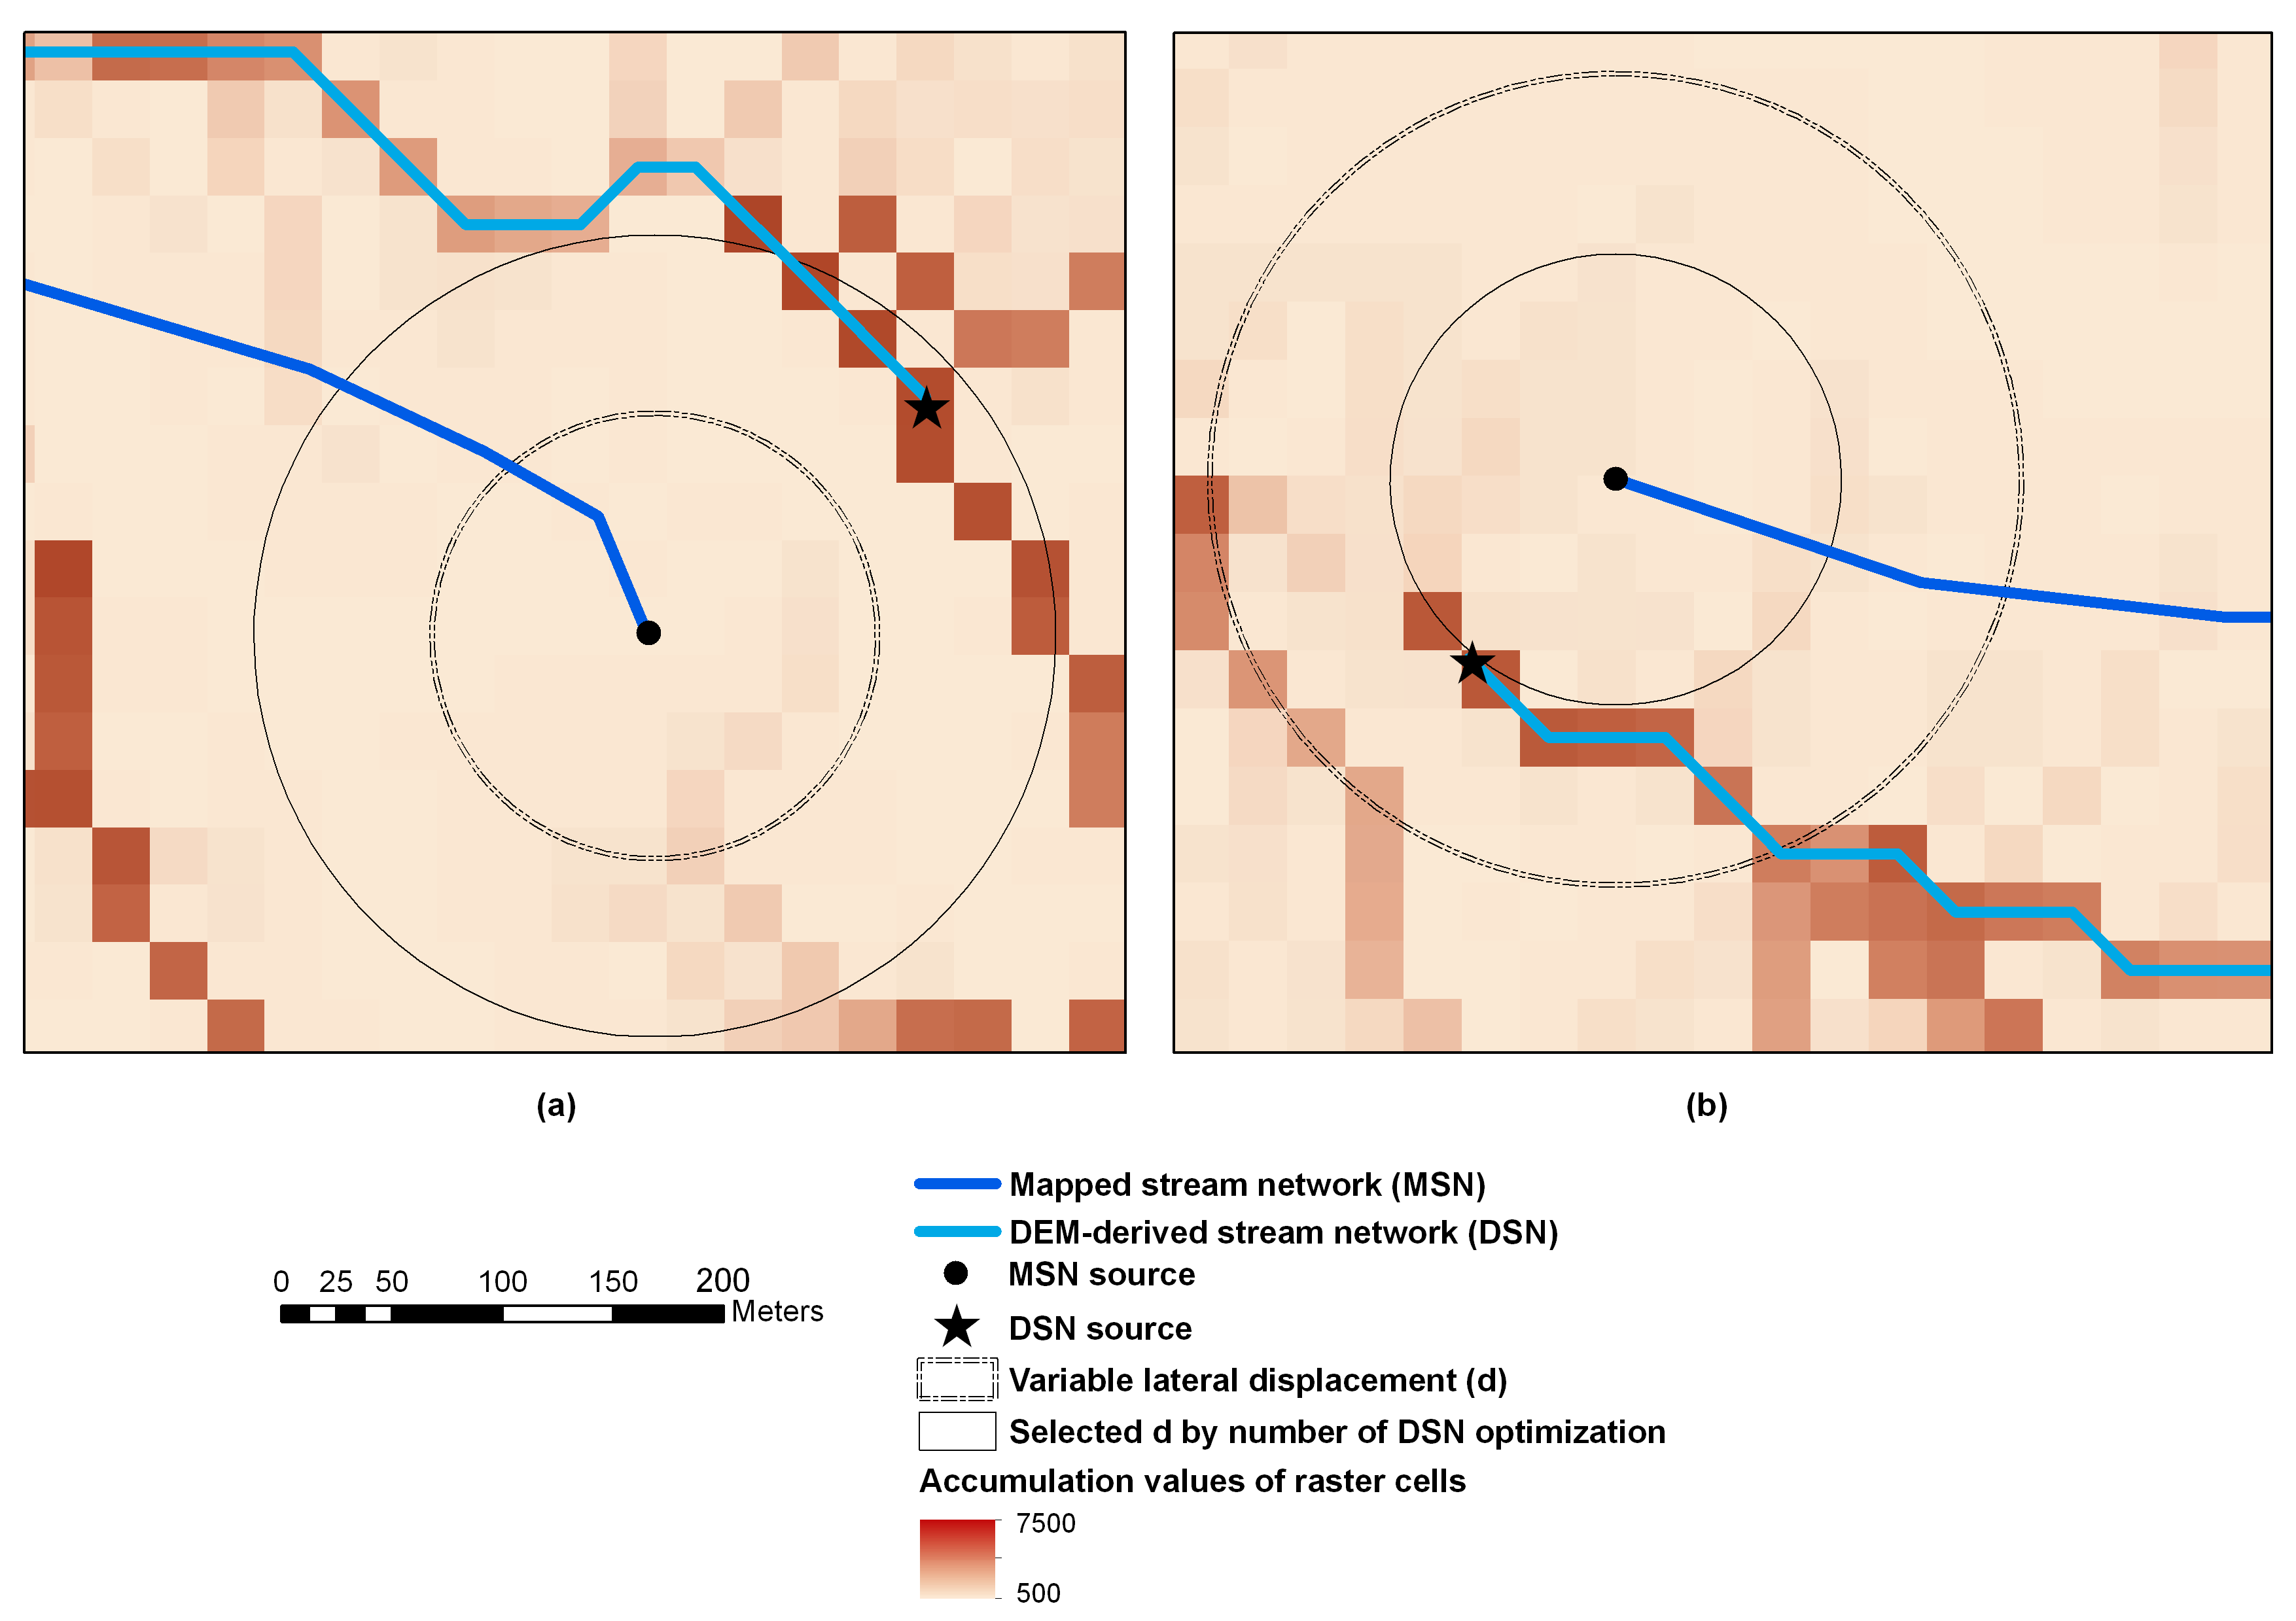
\includegraphics[width=0.71\linewidth]{Figures/Fig_S1_1.png}
  \caption{Variable lateral displacements ($d$) search buffers and selected d by optimizing number of digital elevation model (DEM)-derived stream cells ($n_{DS}$) optimization. When variable $d$s were (a) lower and (b) higher than the selected $d$ a lower and higher accumulation thresholds (AT), respectively, were obtained than the AT obtained by the selected $d$.}
  \label{Fig_A_1}
\end{figure}

\end{landscape}

\begin{figure}[h!]
  \centering
  \hspace{-1cm} 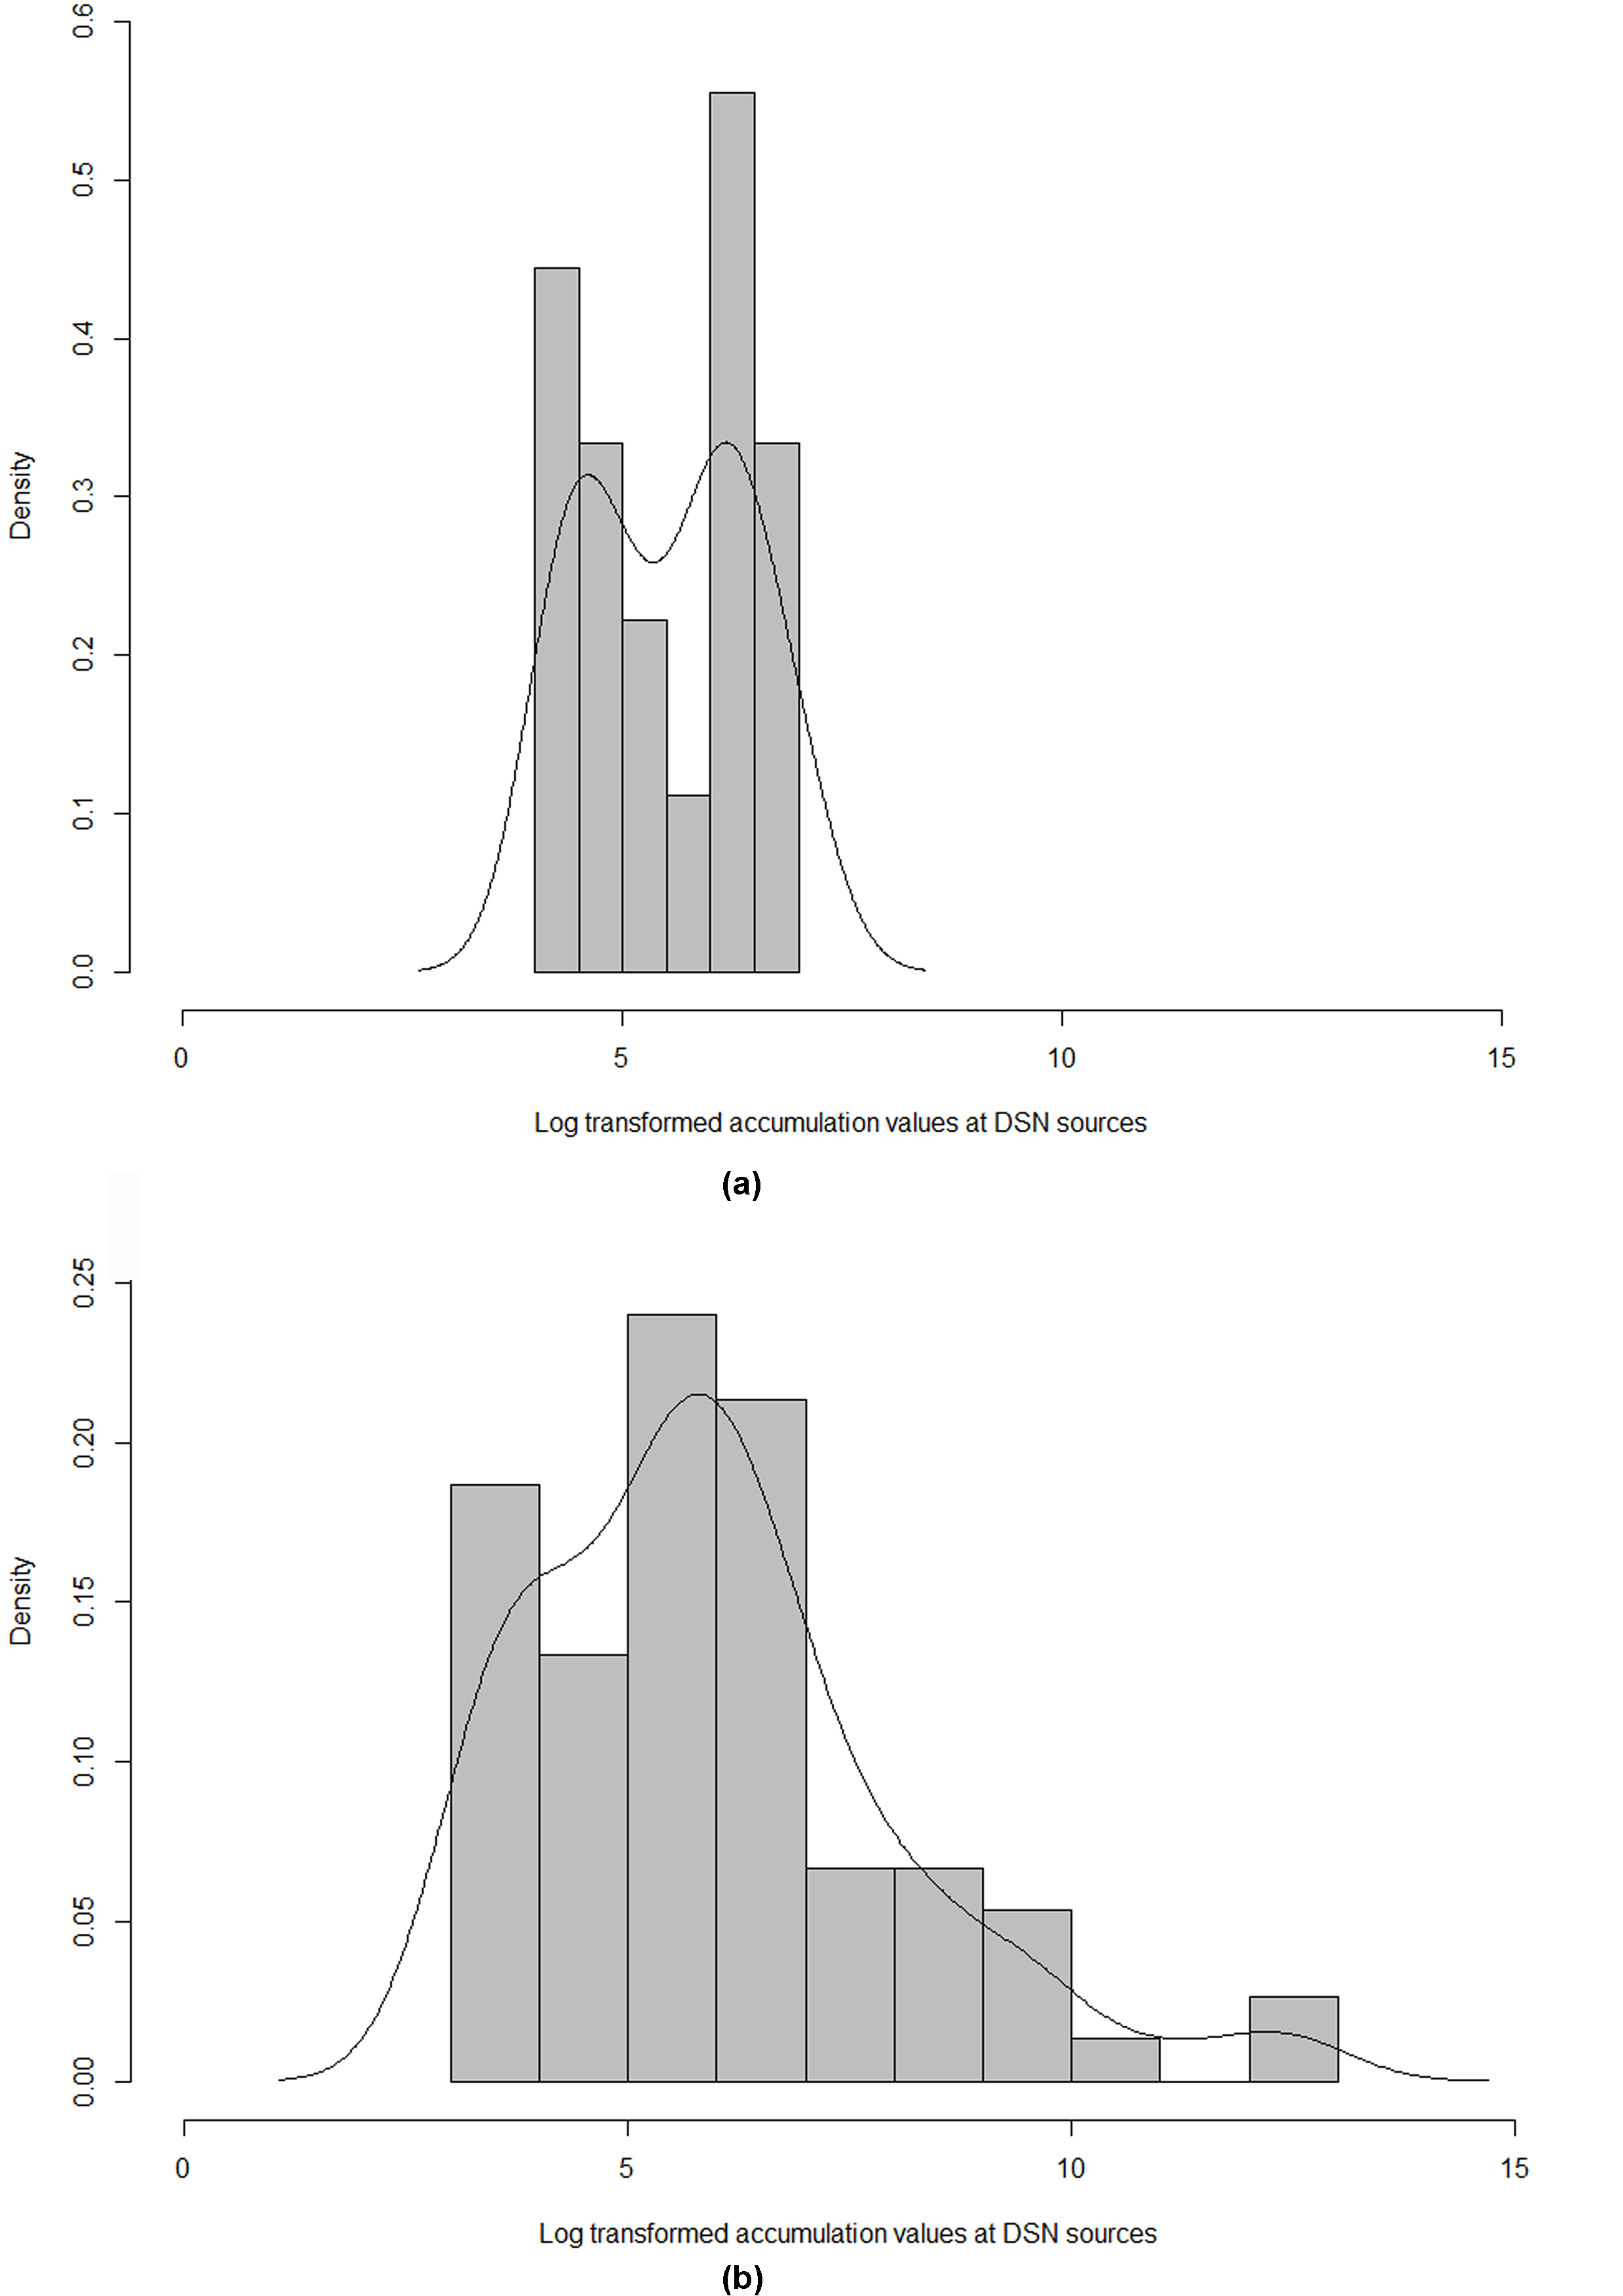
\includegraphics[width=1.1\textwidth]{Figures/Fig_S1_2.png}
  \caption{The histogram and Kernel density plots showing the distribution of the log transformed accumulation values at sources of the digital elevation model (DEM)-derived stream networks (DSN) obtained by the selected lateral displacement ($d$) search buffer in the (a) Hessen watershedand (b) state Thüringen.}
  \label{Fig_A_2}
\end{figure}

\begin{landscape}

\begin{figure}[h!]
  \centering
  \vspace{-1.3cm} 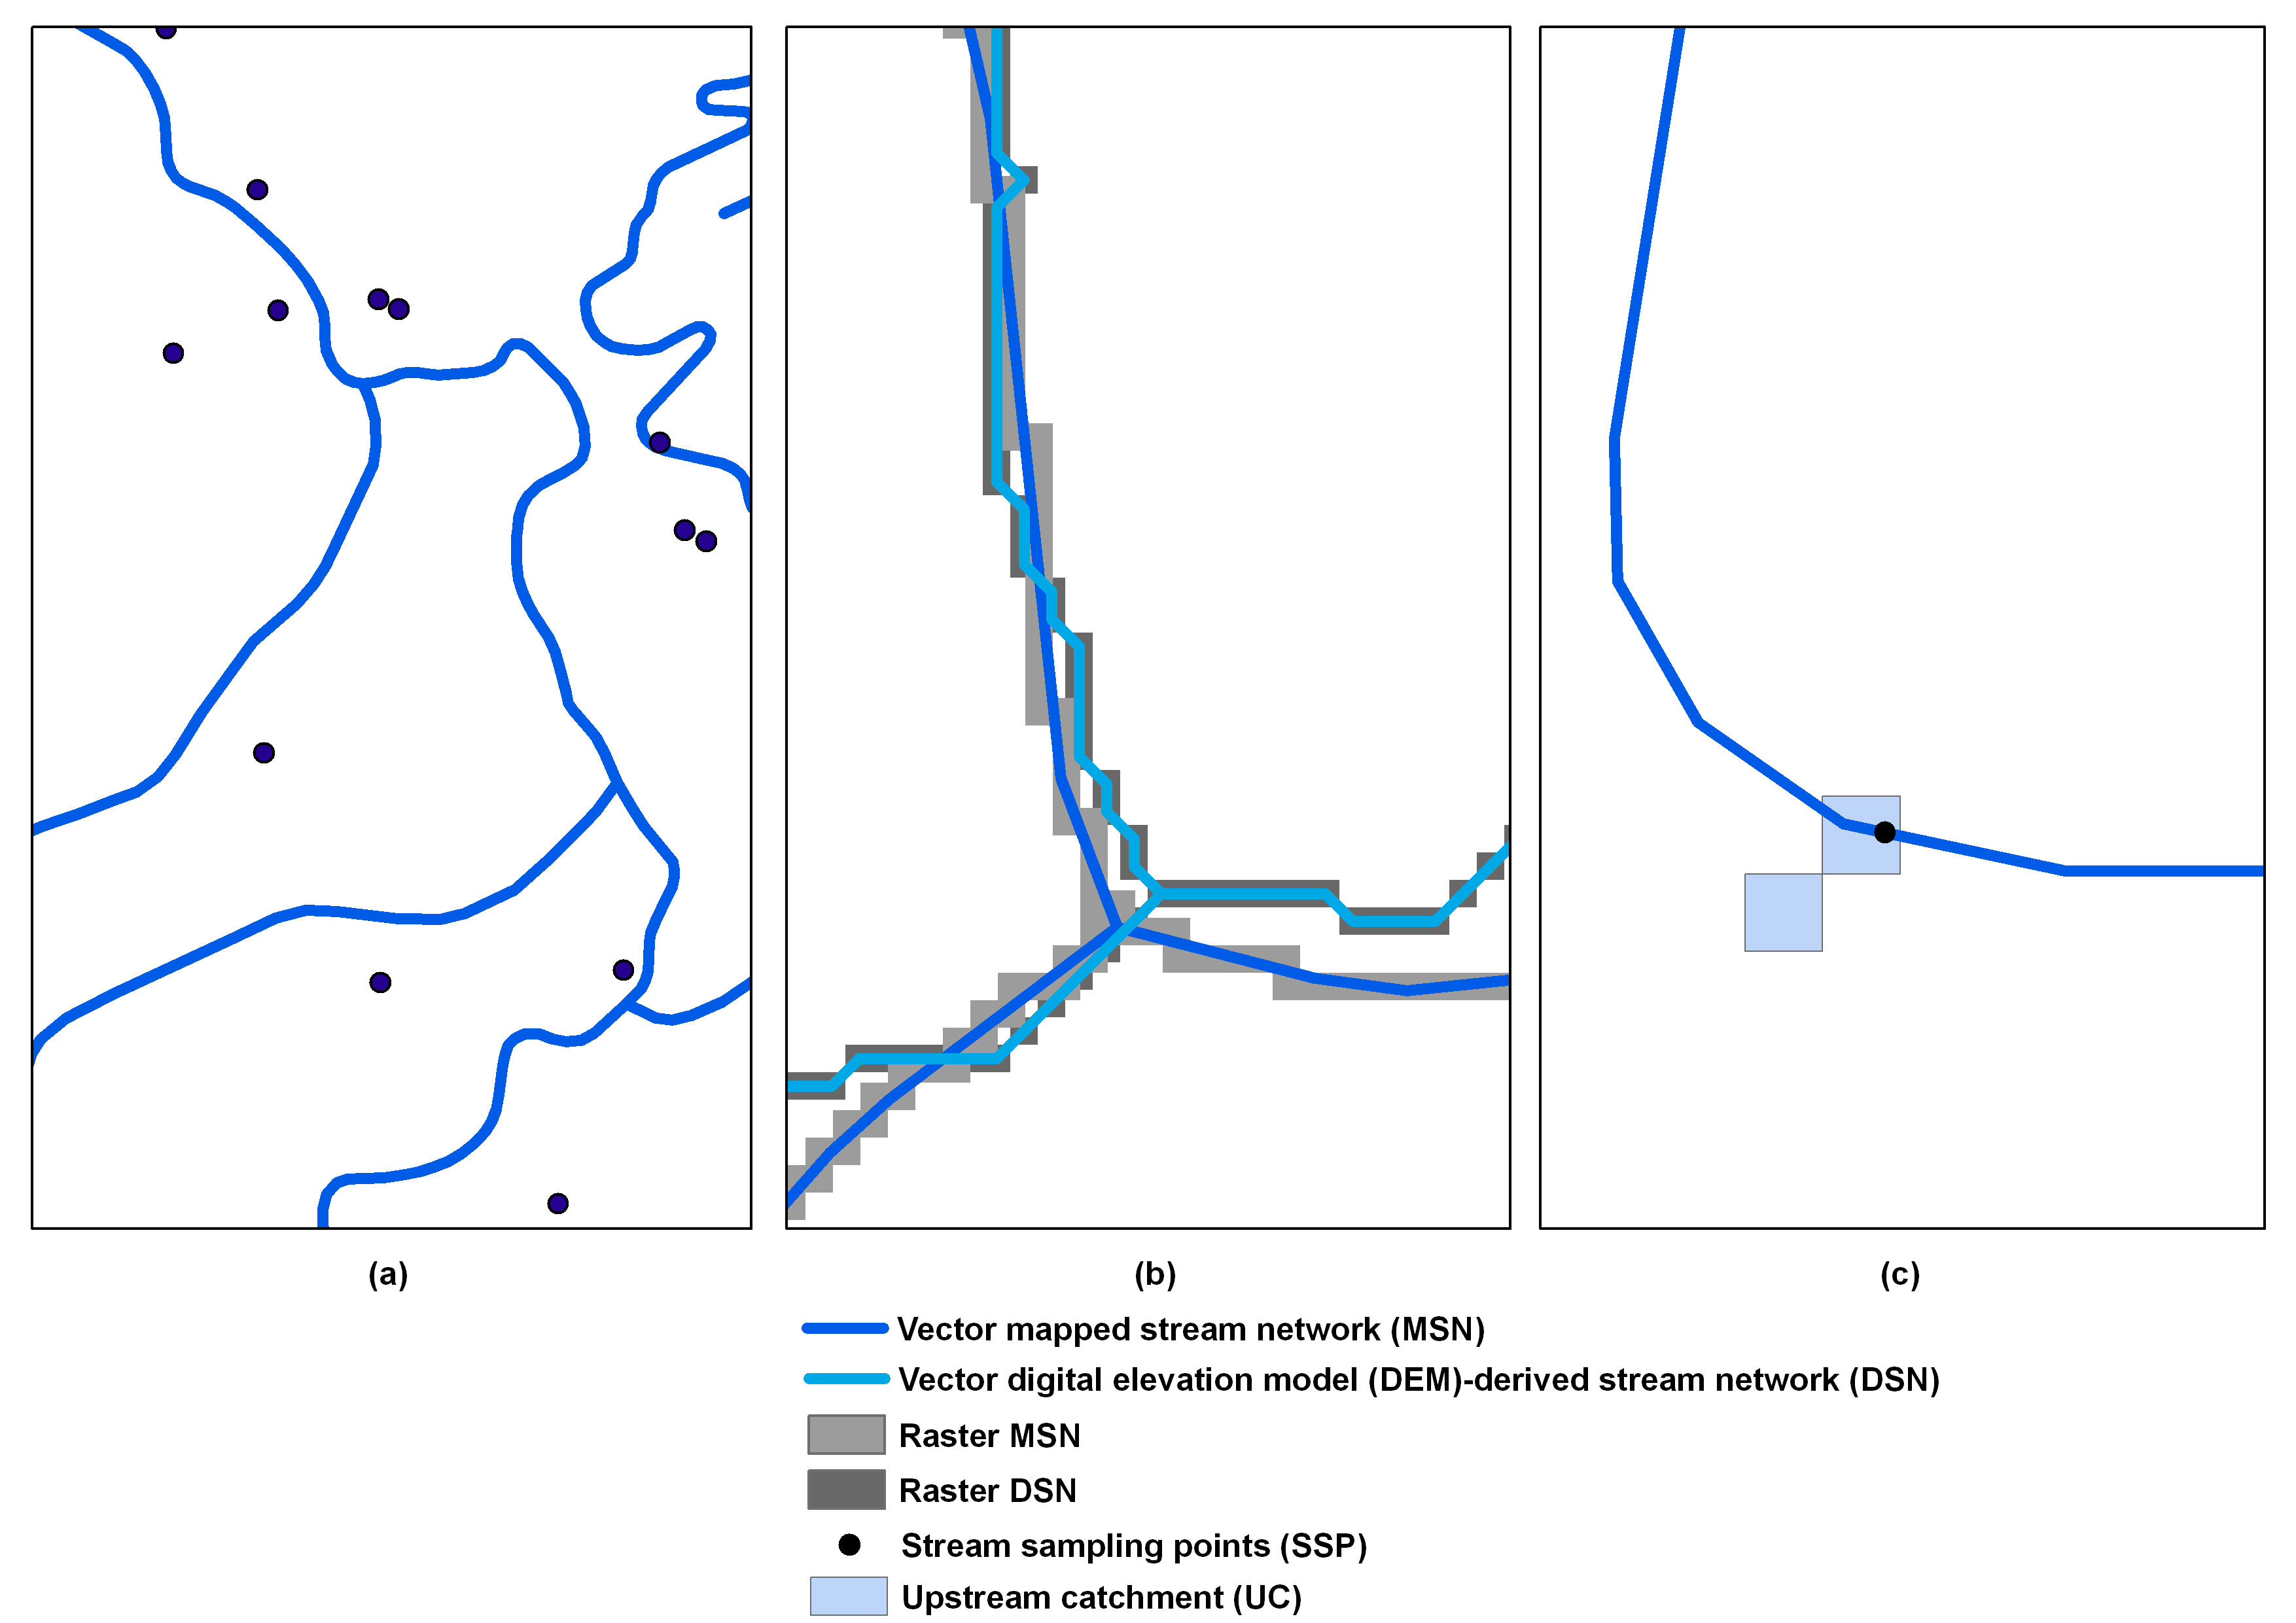
\includegraphics[width=0.9\linewidth]{Figures/Fig_S1_3.png}
  \caption{Lateral displacements observed (a) between given stream sampling points (SSP) and mapped stream network (MSN), (b) between digital elevation model (DEM)-derived  stream network (DSN) and MSN, and (c) delineated scattered and irrelevant upstream catchment for SSP after snapping to MSN.}
  \label{Fig_A_3}
\end{figure}

\end{landscape} % Include the third content chapter
\chapter{Supplementary materials for:\\Spatially shifting temporal points: estimating pooled within-time series variograms for scarce hydrological data}
\label{appendixB}

\section{Supplementary computer code and data}
\label{Supplementary computer code and data}

The computer code along with the reference manual for estimating pooled within-time series (PTS) variograms by applying newly developed spatially shifting temporal points (SSTP), available  averaging empirical variograms (AEV) and a modification of AEV, i.e. weighted averaging empirical variograms (WAEV) methods, is available with the digital version of this thesis and from an online repository: \href{https://github.com/AvitBhowmik/SSTP}{https://github.com/AvitBhowmik/SSTP}. The computer code is an R-script that uses the provided sample data (with the digital version of thesis and the above repository) as input and provides the estimation of PTS variograms by above methods as output. The script was tested using the latest R version 3.2.0 -- ``Full of Ingredients'' that was released on 16.04.2015. Installation of three packages are required: ``spacetime'', ``intamap'' and ``gstat'', where installation of ``intamap'' requires pre-installation of the dependency packages: ``mvtnorm'', ``evd'' and ``sp''. The dependencies may also be automatically installed by R while installing the packages. The installation guideline is provided in the script. Further details and documentations on R and the packages are available from: \href{http://www.r-project.org/}{http://www.r-project.org/}. To get familiar with R, usage examples are available from: \href{http://tryr.codeschool.com/levels/1/challenges/1}{http://tryr.codeschool.com/levels/1/challenges/1}.

The sample data contains computed annual total precipitation in hydrological wet days (PRCPTOT) values at the available data points in Bangladesh for 1993-2007 series. This is a ``STFDF'' data and provided in ``.Rdata'' format. Details on the data format, instructions on how to read and analyze the data are provided in the R-script and package vignettes.

\section{Supplementary figure and table}
\label{Supplementary figure and table}

Figure B.1 illustrates the change in spatial location, distribution and density of the available data points for PRCPTOT in Bangladesh within the 1948-2007 series. A sample of four representative years, i.e. 1948, 1966, 1983 and 2007, is also integrated in Figure 3.3 in chapter 3.

Table B.1 presents the change in the number of available data points and data density, smallest and largets spatial-lags and summary statistics, i.e. minimum, mean, maximum and coefficient of variation of annual total precipitation in hydrological wet days (PRCPTOT) in Bangladesh within the 1948-2007 series. A sample of four representative years, i.e. 1948, 1966, 1983 and 2007, is presented in Figure 3.3 in chapter 3.

\begin{figure*}[h!]
  \centering
  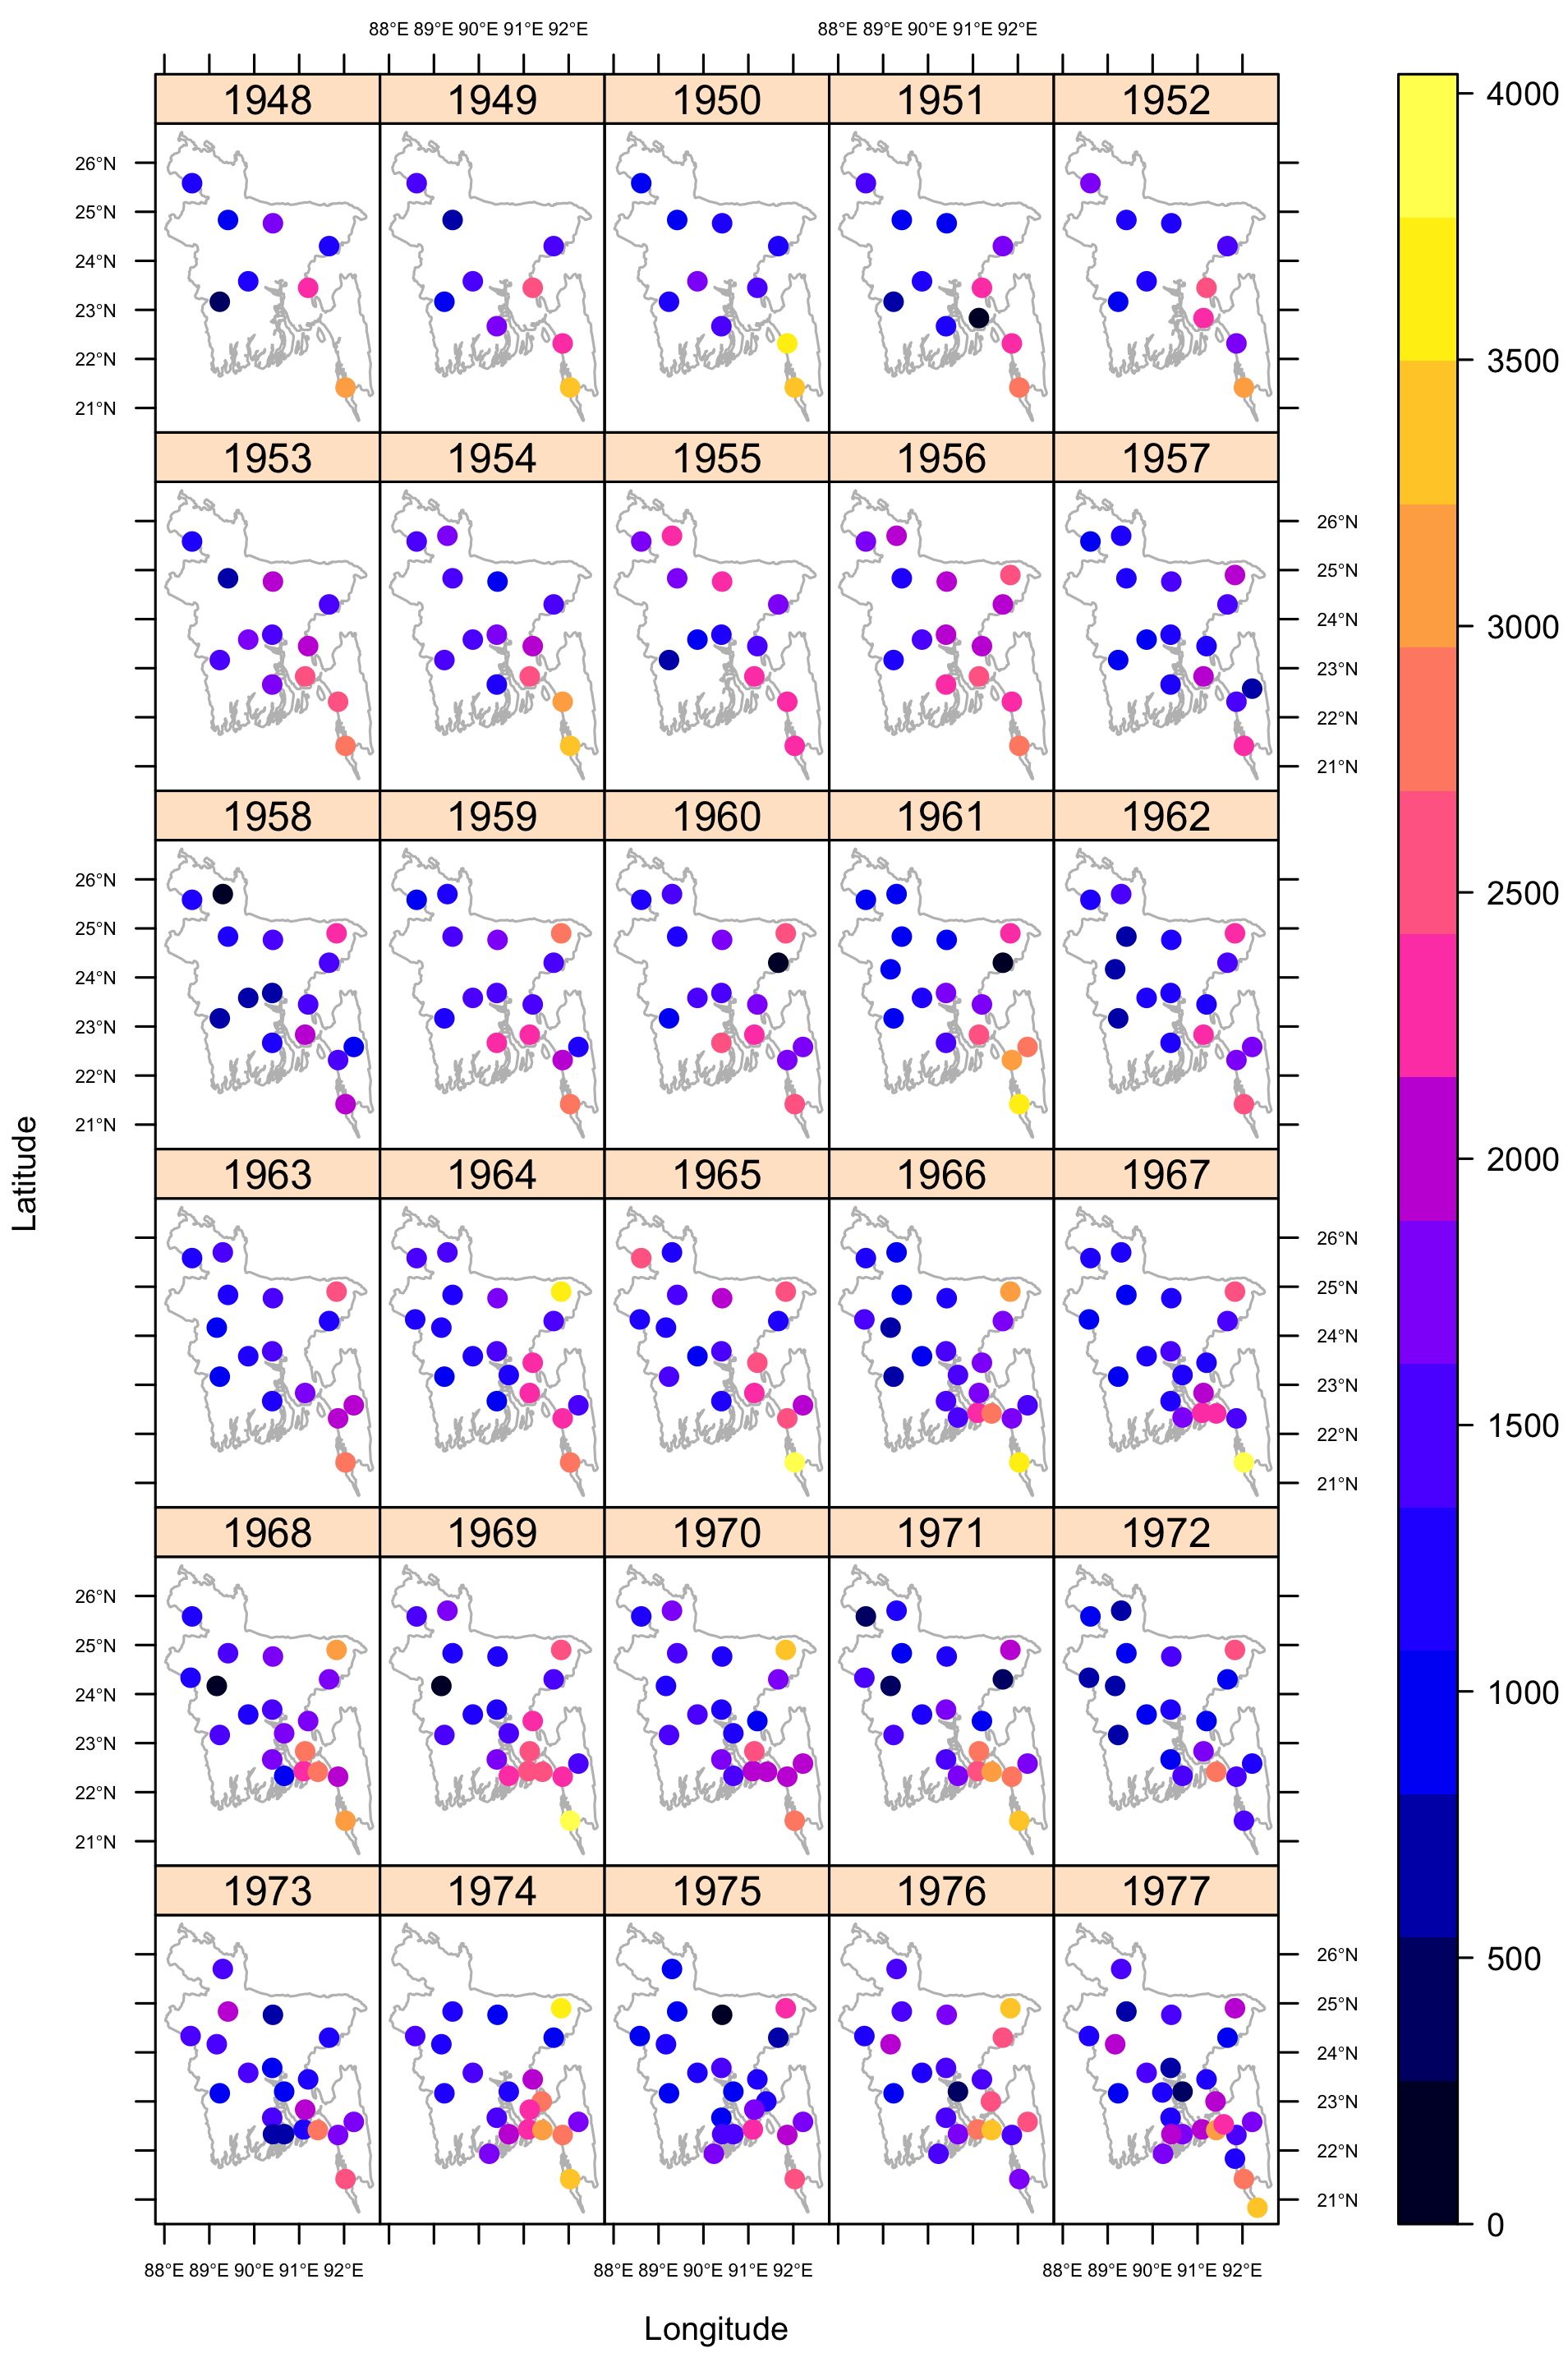
\includegraphics[width=\textwidth]{Figures/Fig_B_1_a.png}
  \label{Fig_B_1_a}
\end{figure*}

\begin{figure}[h!]
  \centering
  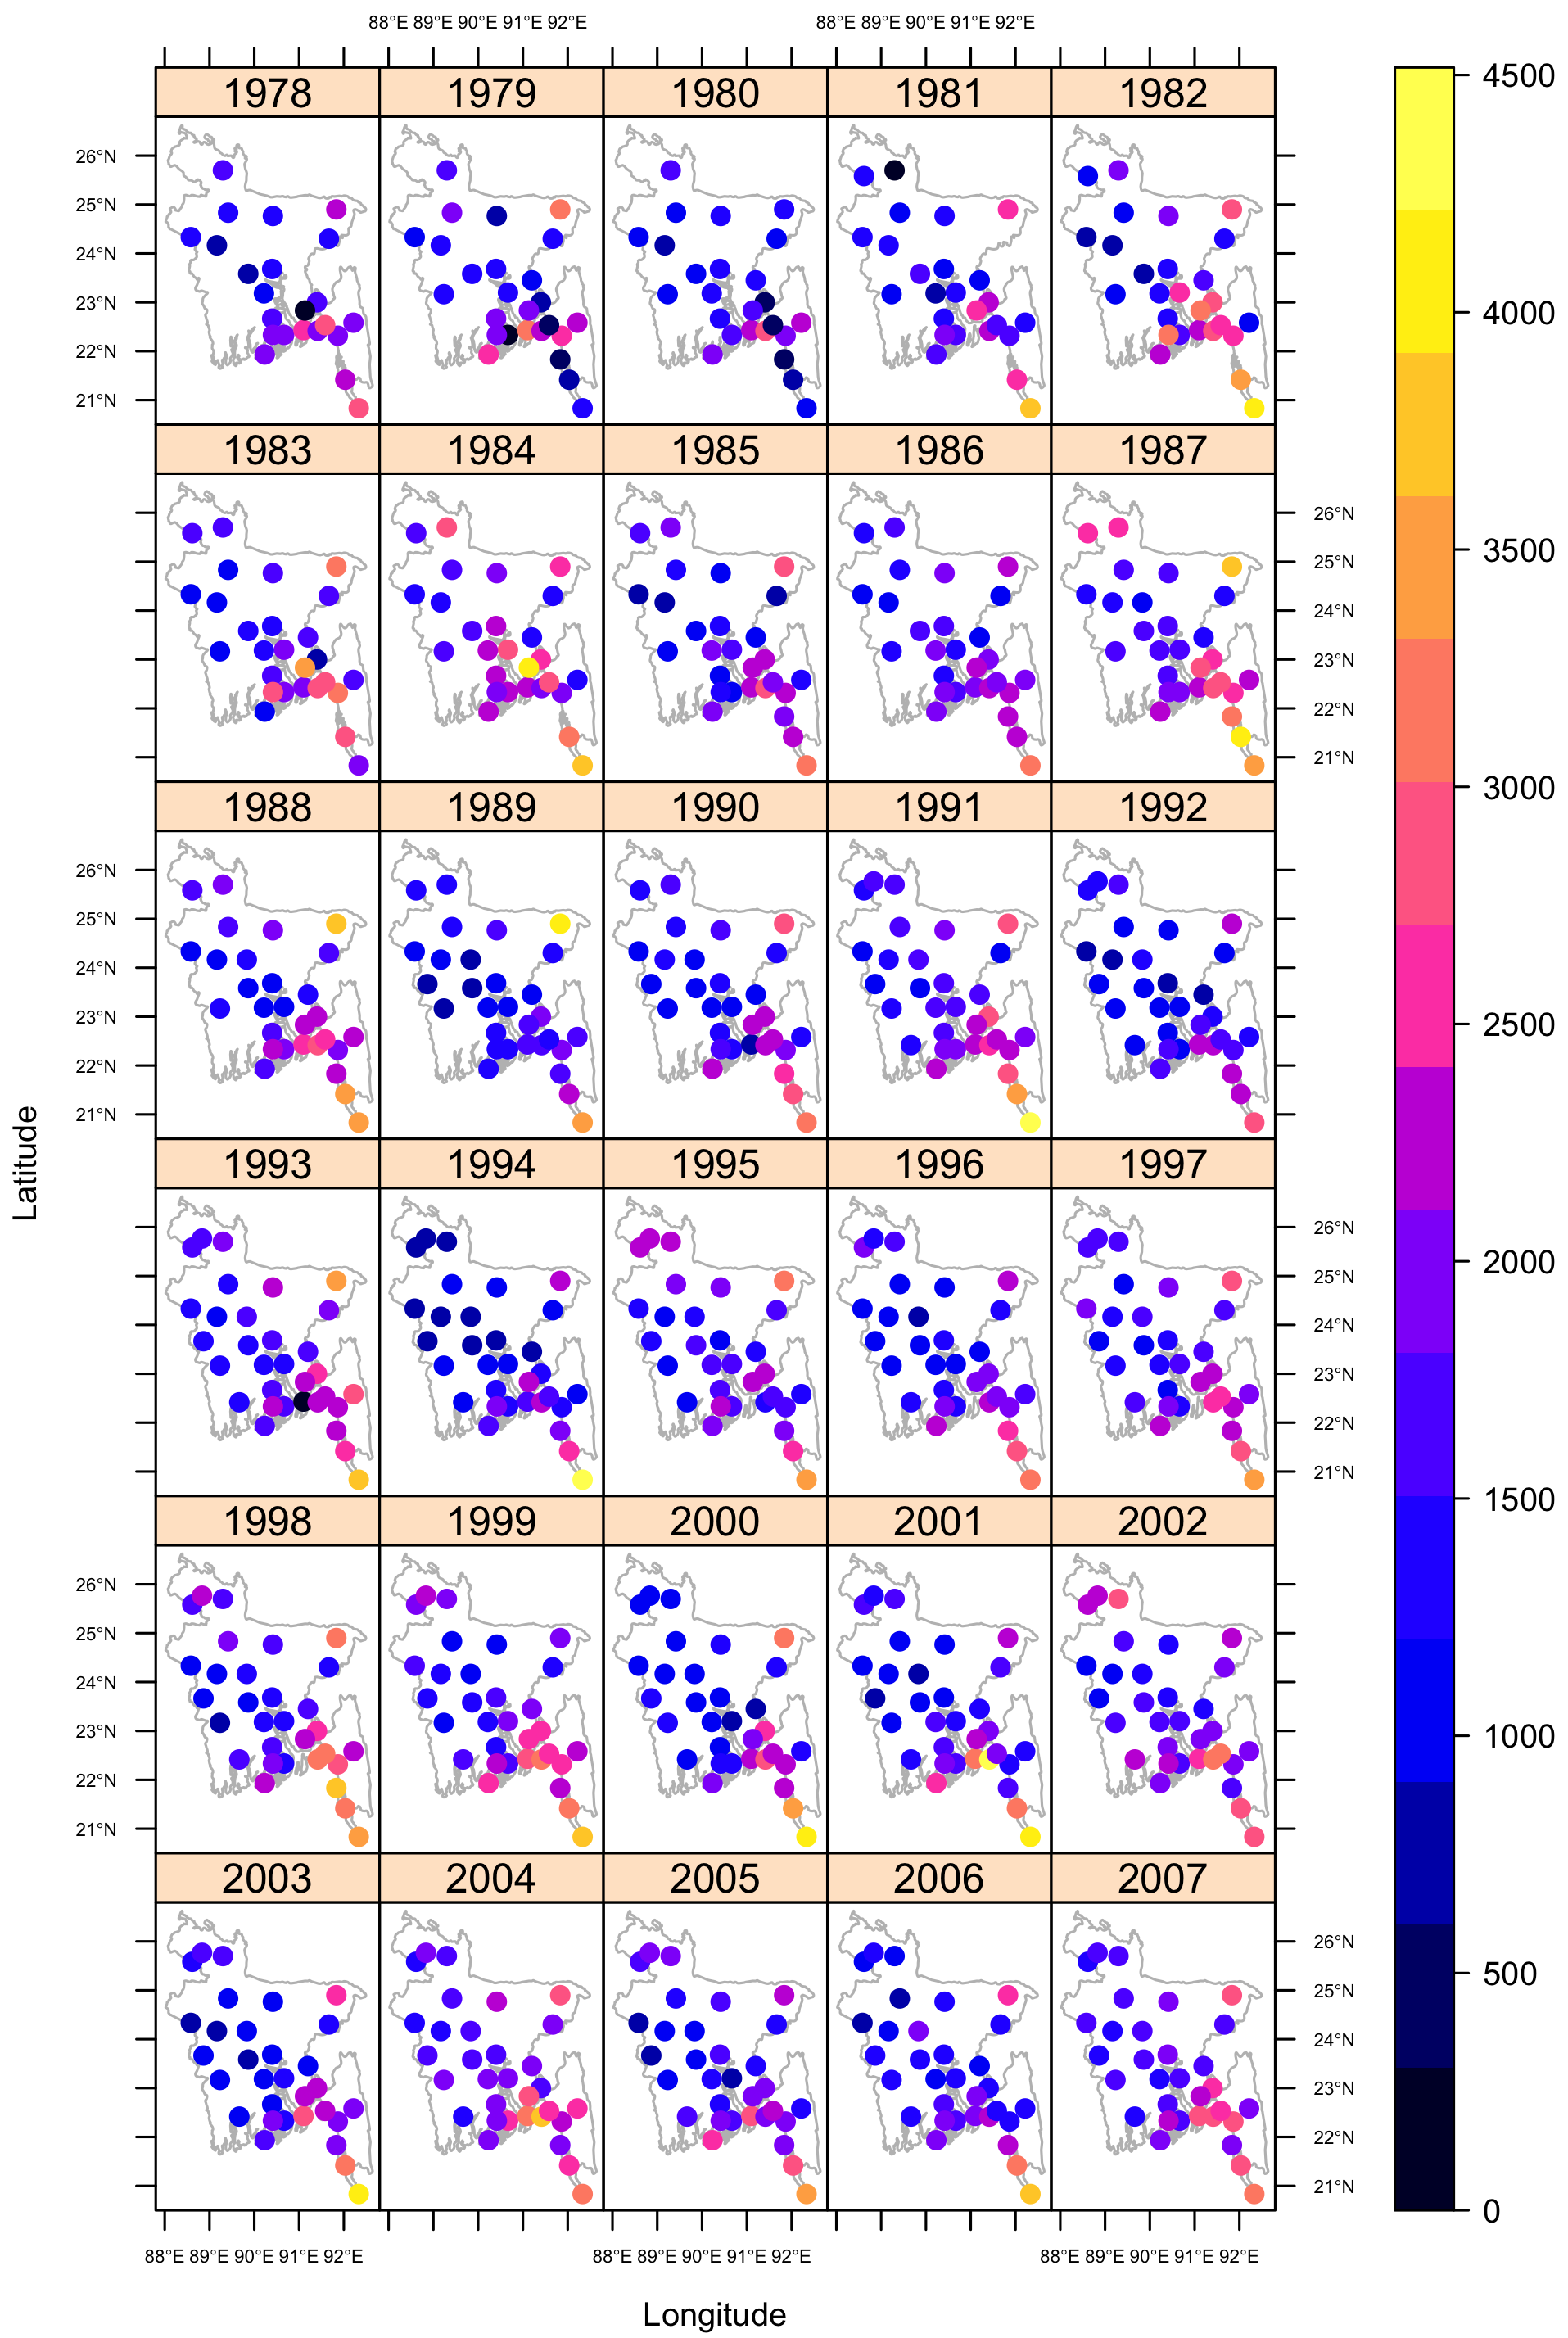
\includegraphics[width=\textwidth]{Figures/Fig_B_1_b.png}
  \caption{Spatial location, distribution and density of available data points (rain-gauge) for each year and annual total precipitation in hydrological wet days (PRCPTOT) (in mm).}
  \label{Fig_B_1_b}
\end{figure}

\clearpage

\setlength{\LTcapwidth}{\linewidth}

\begin{longtable}[c]{>{\centering\arraybackslash}m{0.7cm}>{\centering\arraybackslash}m{2.0cm}>{\centering\arraybackslash}m{2.5cm}>{\centering\arraybackslash}m{1.0cm}>{\centering\arraybackslash}m{1.0cm}>{\centering\arraybackslash}m{0.7cm}>{\centering\arraybackslash}m{0.7cm}>{\centering\arraybackslash}m{0.7cm}>{\centering\arraybackslash}m{0.7cm}}

\caption{Number of available data points, data point density, smallest and largest spatial-lags, and minimum (min.), mean, maximum (max.) and coefficient of variation (CV) of annual total precipitation in hydrological wet days (PRCPTOT) in Bangladesh for each time step (year) within 1948-2007 series.}

\hline
\textbf{Year} & \textbf{Available number of data points} & \textbf{Data point density} & \multicolumn{2}{c}{\textbf{Spatial lag}} & \multicolumn{4}{c}{\textbf{PRCPTOT}}\\
 & & & \textbf{Smallest} & \textbf{Largest} & \textbf{Min.} & \textbf{Mean} & \textbf{Max.} & \textbf{CV}\\
 & & \textbf{(point/10000 $km^2$)} & \textbf{$(km)$} & \textbf{$(km)$} & \textbf{$(mm)$} & \textbf{$(mm)$} & \textbf{$(mm)$} & \textbf{(\%)}\\
\hline
\endfirsthead

\hline
\endhead

\hline
\endfoot

1948 & 8 & 0.5 & 95.38 & 489.85 & 494 & 1532 & 3028 & 53.59\\
1949 & 9 & 0.6 & 95.22 & 489.85 & 574 & 1772 & 3369 & 47.40\\
1950 & 10 & 0.7 & 96.76 & 489.85 & 981 & 1708 & 3521 & 54.98\\
1951 & 11 & 0.7 & 68.57 & 489.85 & 225 & 1447 & 2916 & 53.77\\
1952 & 10 & 0.7 & 68.57 & 489.85 & 972 & 1778 & 3131 & 37.96\\
1953 & 12 & 0.8 & 62.08 & 489.85 & 671 & 1818 & 2813 & 32.95\\
1954 & 13 & 0.9 & 64.69 & 549.70 & 1006 & 1876 & 3378 & 36.73\\
1955 & 12 & 0.8 & 64.69 & 549.70 & 779 & 1744 & 2374 & 31.25\\
1956 & 14 & 0.9 & 65.64 & 549.70 & 1214 & 2016 & 2913 & 24.55\\
1957 & 15 & 1.0 & 61.83 & 549.70 & 651 & 1334 & 2324 & 33.51\\
1958 & 15 & 1.0 & 61.83 & 549.70 & 188 & 1263 & 2185 & 46.63\\
1959 & 15 & 1.0 & 61.83 & 549.70 & 859 & 1754 & 2888 & 34.38\\
1960 & 14 & 0.9 & 61.83 & 549.70 & 999 & 1763 & 2622 & 30.80\\
1961 & 15 & 1.0 & 61.83 & 549.70 & 878 & 1765 & 3617 & 51.61\\
1962 & 16 & 1.1 & 61.83 & 549.70 & 723 & 1447 & 2510 & 36.97\\
1963 & 15 & 1.0 & 60.14 & 549.70 & 967 & 1571 & 2839 & 36.03\\
1964 & 18 & 1.2 & 62.00 & 549.70 & 938 & 1690 & 3530 & 40.71\\
1965 & 17 & 1.2 & 61.86 & 549.70 & 1050 & 1860 & 4036 & 42.58\\
1966 & 21 & 1.4 & 32.57 & 549.70 & 767 & 1648 & 3694 & 46.48\\
1967 & 19 & 1.3 & 32.57 & 549.70 & 850 & 1601 & 3836 & 46.16\\
1968 & 18 & 1.2 & 32.57 & 484.33 & 1001 & 1892 & 3132 & 35.15\\
1969 & 19 & 1.3 & 32.57 & 549.70 & 1080 & 1930 & 3872 & 36.84\\
1970 & 20 & 1.4 & 32.57 & 549.70 & 952 & 1761 & 3315 & 34.87\\
1971 & 20 & 1.4 & 32.57 & 549.70 & 389 & 1662 & 3489 & 53.31\\
1972 & 19 & 1.3 & 59.25 & 549.70 & 740 & 1259 & 2856 & 45.51\\
1973 & 20 & 1.4 & 29.16 & 549.70 & 545 & 1435 & 2785 & 40.07\\
1974 & 20 & 1.4 & 32.80 & 478.82 & 849 & 1932 & 3710 & 43.27\\
1975 & 22 & 1.5 & 29.39 & 549.70 & 17 & 1353 & 2519 & 43.83\\
1976 & 21 & 1.4 & 32.57 & 549.70 & 329 & 1840 & 3371 & 42.07\\
1977 & 26 & 1.8 & 26.61 & 543.36 & 430 & 1654 & 3271 & 44.14\\
1978 & 23 & 1.6 & 28.22 & 543.36 & 84 & 1697 & 2853 & 39.48\\
1979 & 25 & 1.7 & 28.22 & 543.36 & 424 & 1615 & 3126 & 46.25\\
1980 & 25 & 1.7 & 29.04 & 543.36 & 327 & 1327 & 2758 & 44.84\\
1981 & 25 & 1.7 & 26.77 & 543.36 & 104 & 1629 & 3649 & 44.75\\
1982 & 27 & 1.8 & 28.22 & 543.36 & 732 & 1981 & 3976 & 47.10\\
1983 & 27 & 1.8 & 28.22 & 543.36 & 640 & 1822 & 3326 & 42.48\\
1984 & 27 & 1.8 & 28.22 & 543.36 & 1237 & 2182 & 4010 & 32.81\\
1985 & 28 & 1.9 & 28.22 & 539.70 & 701 & 1667 & 3230 & 39.59\\
1986 & 28 & 1.9 & 28.22 & 539.70 & 1081 & 1787 & 3133 & 26.13\\
1987 & 29 & 2.0 & 28.22 & 539.70 & 1124 & 2204 & 4076 & 36.16\\
1988 & 29 & 2.0 & 28.22 & 539.70 & 951 & 1959 & 3626 & 37.98\\
1989 & 30 & 2.0 & 28.22 & 549.70 & 675 & 1508 & 3958 & 47.28\\
1990 & 30 & 2.0 & 28.22 & 549.70 & 747 & 1656 & 3093 & 39.07\\
1991 & 32 & 2.2 & 28.52 & 538.09 & 1077 & 1960 & 4499 & 37.55\\
1992 & 32 & 2.2 & 28.52 & 538.09 & 638 & 1395 & 2849 & 39.57\\
1993 & 32 & 2.2 & 28.52 & 538.09 & 29 & 1873 & 3722 & 36.73\\
1994 & 32 & 2.2 & 28.52 & 538.09 & 696 & 1366 & 4261 & 53.88\\
1995 & 31 & 2.1 & 27.51 & 538.09 & 1033 & 1800 & 3528 & 32.17\\
1996 & 31 & 2.1 & 27.51 & 538.09 & 779 & 1613 & 3185 & 38.31\\
1997 & 31 & 2.1 & 27.51 & 538.09 & 962 & 1840 & 3346 & 32.61\\
1998 & 31 & 2.1 & 27.51 & 538.09 & 727 & 1948 & 3752 & 42.04\\
1999 & 32 & 2.2 & 28.52 & 538.09 & 961 & 2015 & 3661 & 34.14\\
2000 & 32 & 2.2 & 28.52 & 538.09 & 868 & 1637 & 3919 & 49.42\\
2001 & 32 & 2.2 & 28.52 & 538.09 & 818 & 1765 & 4516 & 51.05\\
2002 & 32 & 2.2 & 28.52 & 538.09 & 1016 & 1940 & 3186 & 29.74\\
2003 & 31 & 2.1 & 29.51 & 538.09 & 719 & 1621 & 4024 & 48.12\\
2004 & 32 & 2.2 & 28.52 & 538.09 & 1386 & 2117 & 3889 & 28.25\\
2005 & 32 & 2.2 & 28.52 & 538.09 & 708 & 1702 & 3605 & 37.84\\
2006 & 32 & 2.2 & 28.52 & 538.09 & 688 & 1604 & 3697 & 40.27\\
2007 & 32 & 2.2 & 28.52 & 538.09 & 1290 & 1993 & 3271 & 28.55\\

\end{longtable} % Include the third content chapter
\chapter{Supplementary materials for:\\Large scale relationship between aquatic insect traits and climate}
\label{appendixC}

\section{Supplementary figures}
\label{Supplementary figures}

See next page.

\newpage

\begin{figure*}[hp!]
  \centering
  \hspace{-2cm} 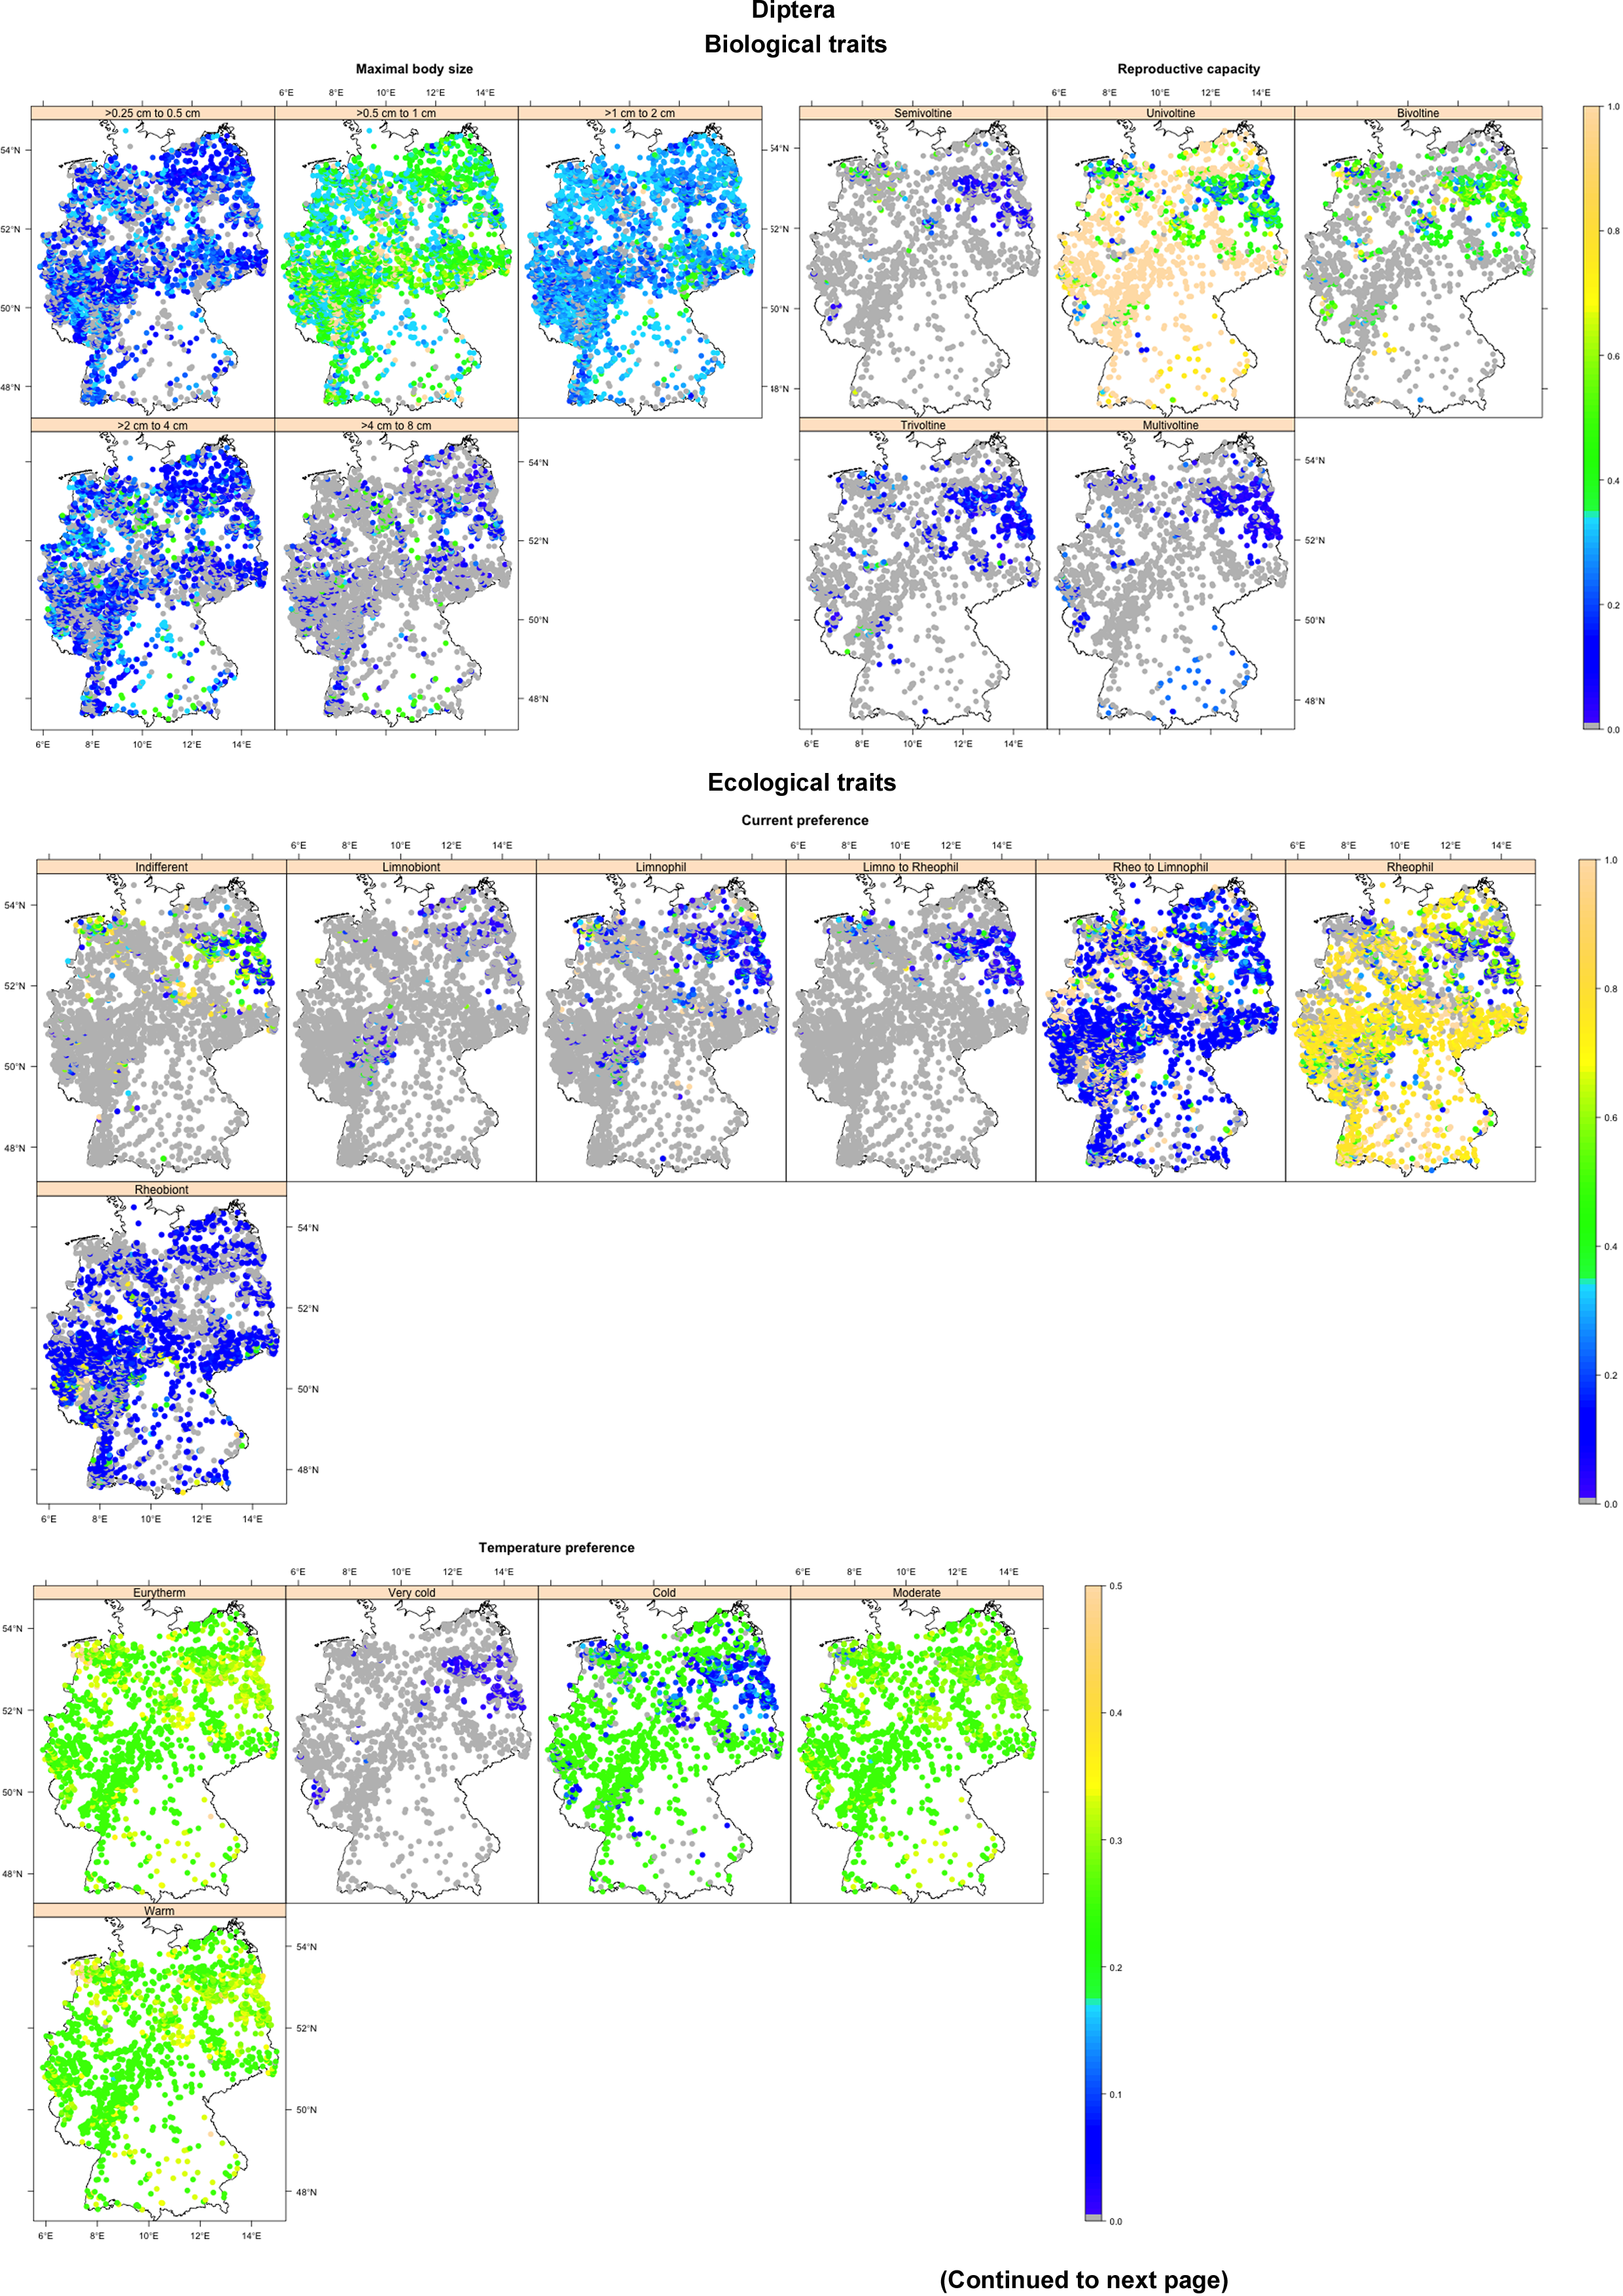
\includegraphics[width=1.1\textwidth]{Figures/Fig_C_1_a.png}
  \label{Fig_C_1_a}
\end{figure*}

\newpage

\begin{figure*}[hp!]
  \centering
  \includegraphics[width=1.1\textwidth]{Figures/Fig_C_1_b.png}
  \label{Fig_C_1_b}
\end{figure*}

\newpage

\begin{figure*}[hp!]
  \centering
  \hspace{-2cm}\includegraphics[width=1.1\textwidth]{Figures/Fig_C_1_c.png}
  \label{Fig_C_1_c}
\end{figure*}

\newpage

\begin{figure}[hp!]
  \centering
  \includegraphics[width=1.1\textwidth]{Figures/Fig_C_1_d.png}
  \caption{Annual averaged abundance weighted traits across 4,752 stream sites in Germany for each order. The figure captions, sub-captions and panel captions indicate the names of orders, grouping features and traits, respectively. The gray dots indicate zero abundance, i.e. trait absence.}
  \label{Fig_C_1_d}
\end{figure}

\newpage

\begin{figure*}[hp!]
  \centering
  \hspace{-2cm}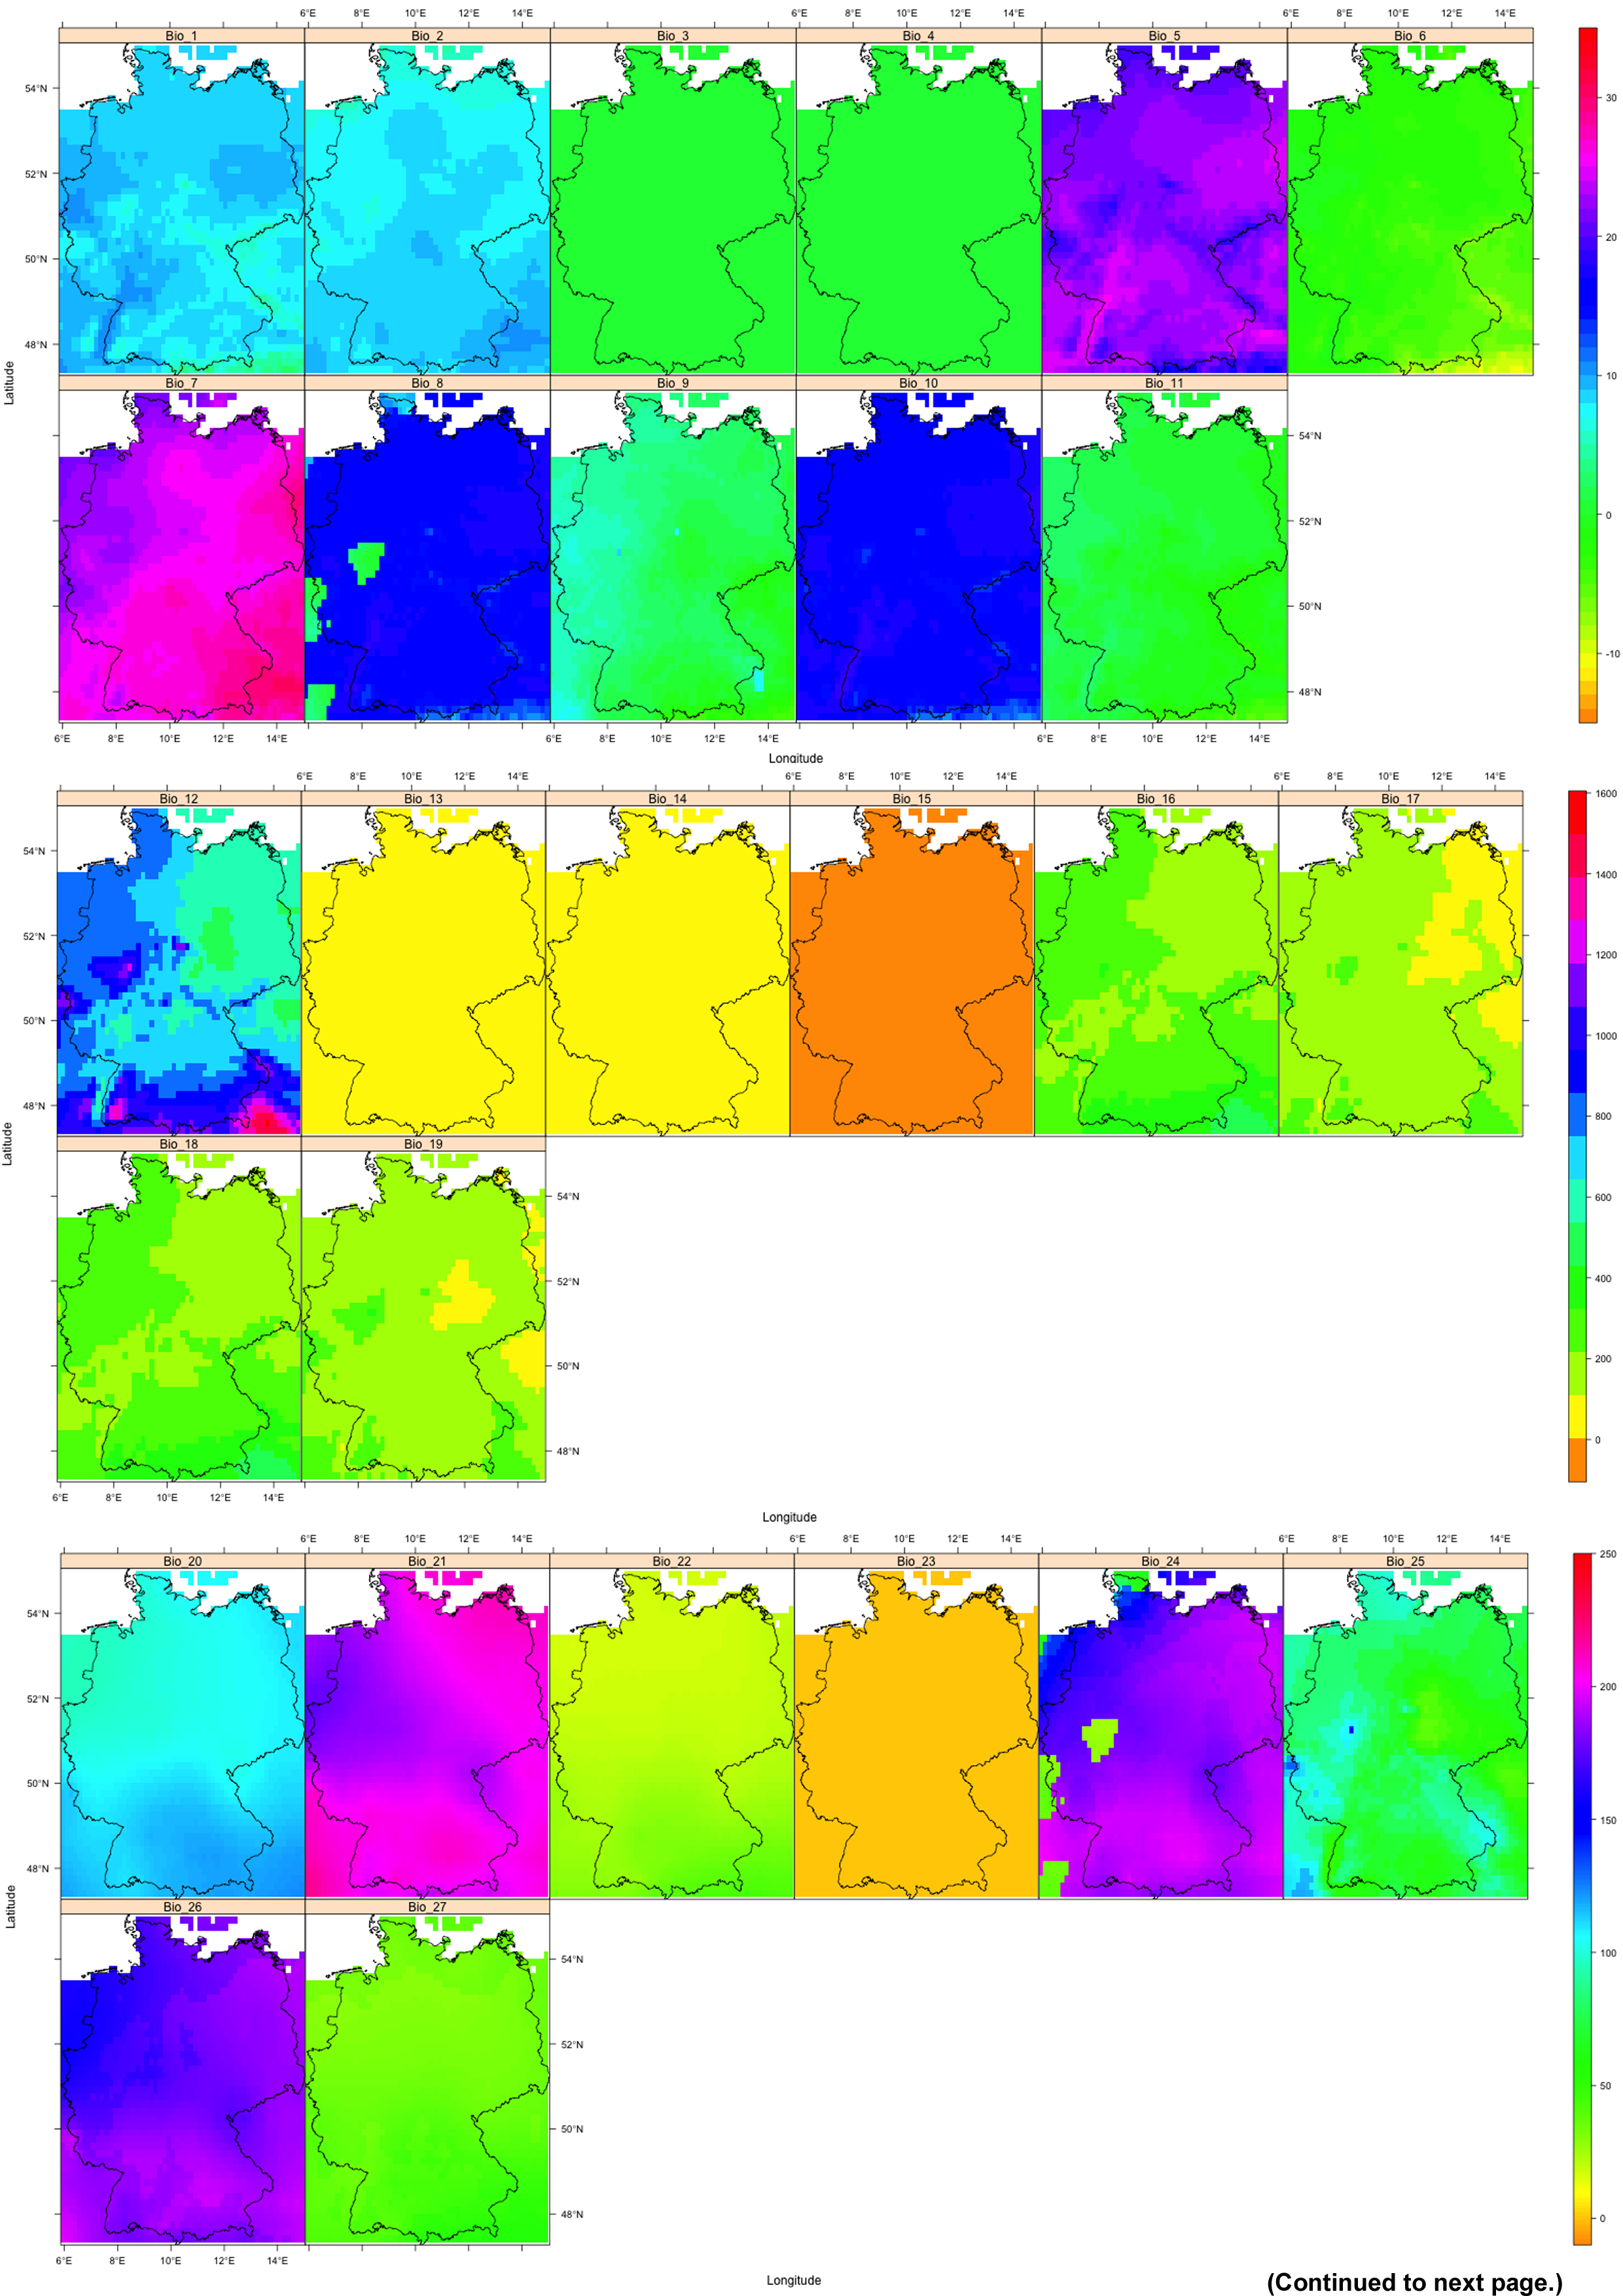
\includegraphics[width=1.1\textwidth]{Figures/Fig_C_2_a.png}
  \label{Fig_C_2_a}
\end{figure*}

\clearpage

\begin{figure}[h!]
  \centering
  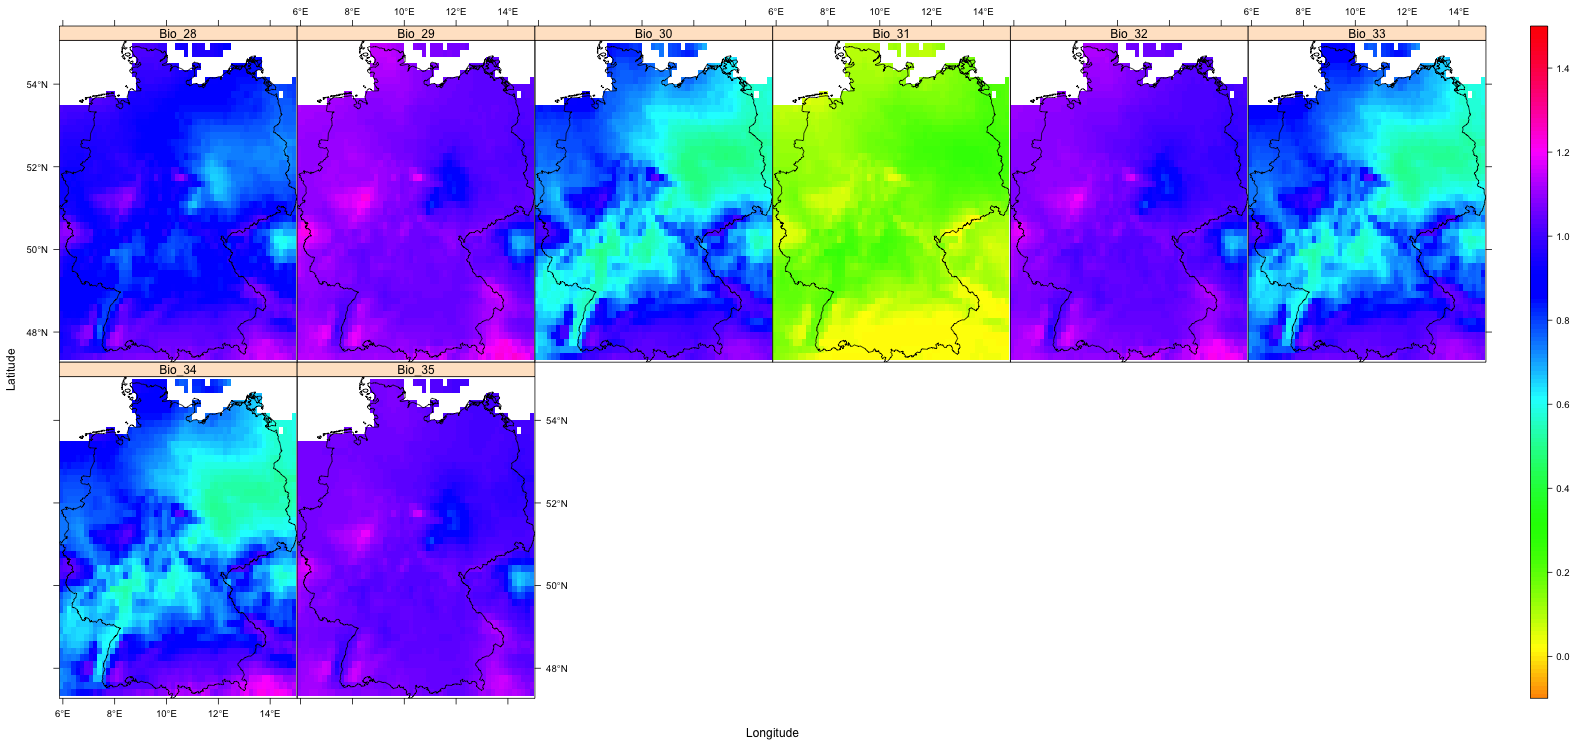
\includegraphics[width=\textwidth]{Figures/Fig_C_2_b.png}
  \caption{Extracted 35 global bioclimatic indices within the border of Germany. The indices are grouped according to their value ranges and units (\textsuperscript{0}C, mm, W m\textsuperscript{-2} and no unit). The panel captions indicate the IDs of the indices (Bio\textunderscore ID). Details on the indices and their IDs and units can be found in Table 2 and \href{https://www.climond.org/Resources.aspx}{https://www.climond.org/Resources.aspx}.}
  \label{Fig_C_2_b}
\end{figure}

\newpage

\begin{figure}[h!]
  \centering
  \captionsetup{width=1.1\textwidth}
  \hspace{-2cm}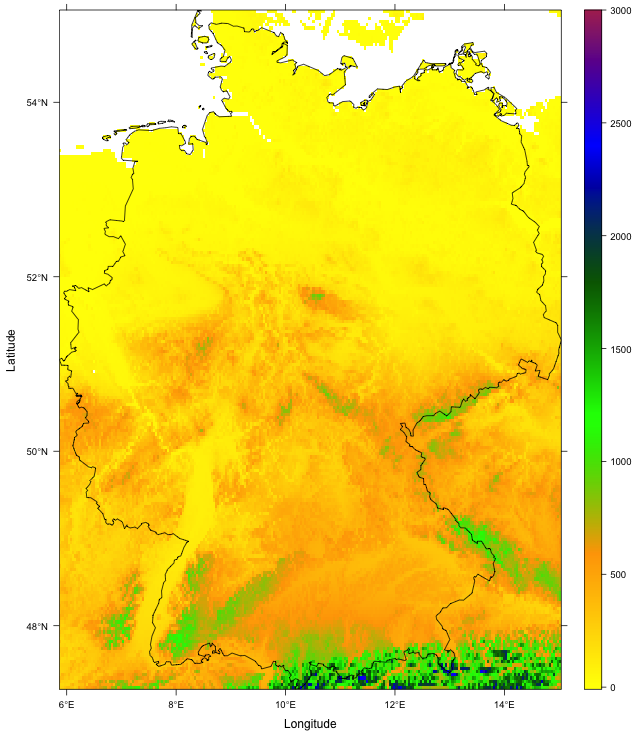
\includegraphics[width=1.1\textwidth]{Figures/Fig_C_3.png}
  \caption{Altitudes from the mean sea level (m) within the border of Germany. Details can be found in \href{http://asterweb.jpl.nasa.gov/gdem.asp}{http://asterweb.jpl.nasa.gov/gdem.asp}.}
  \label{Fig_C_3}
\end{figure}

\clearpage

\begin{figure}[hp!]
  \centering
  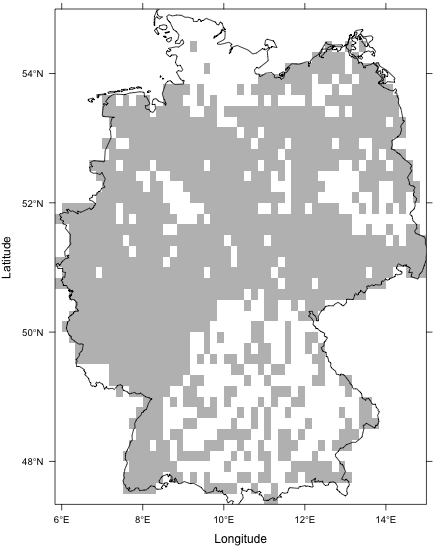
\includegraphics[width=\textwidth]{Figures/Fig_C_4.png}
  \caption{Bioclimatic indices (BIs) raster cells that are covered (72 \%) by the bio-monitoring steam sites.}
  \label{Fig_C_4}
\end{figure}

\clearpage

\begin{landscape}

\begin{figure}[h!]
  \centering
  \vspace{-2.3cm} 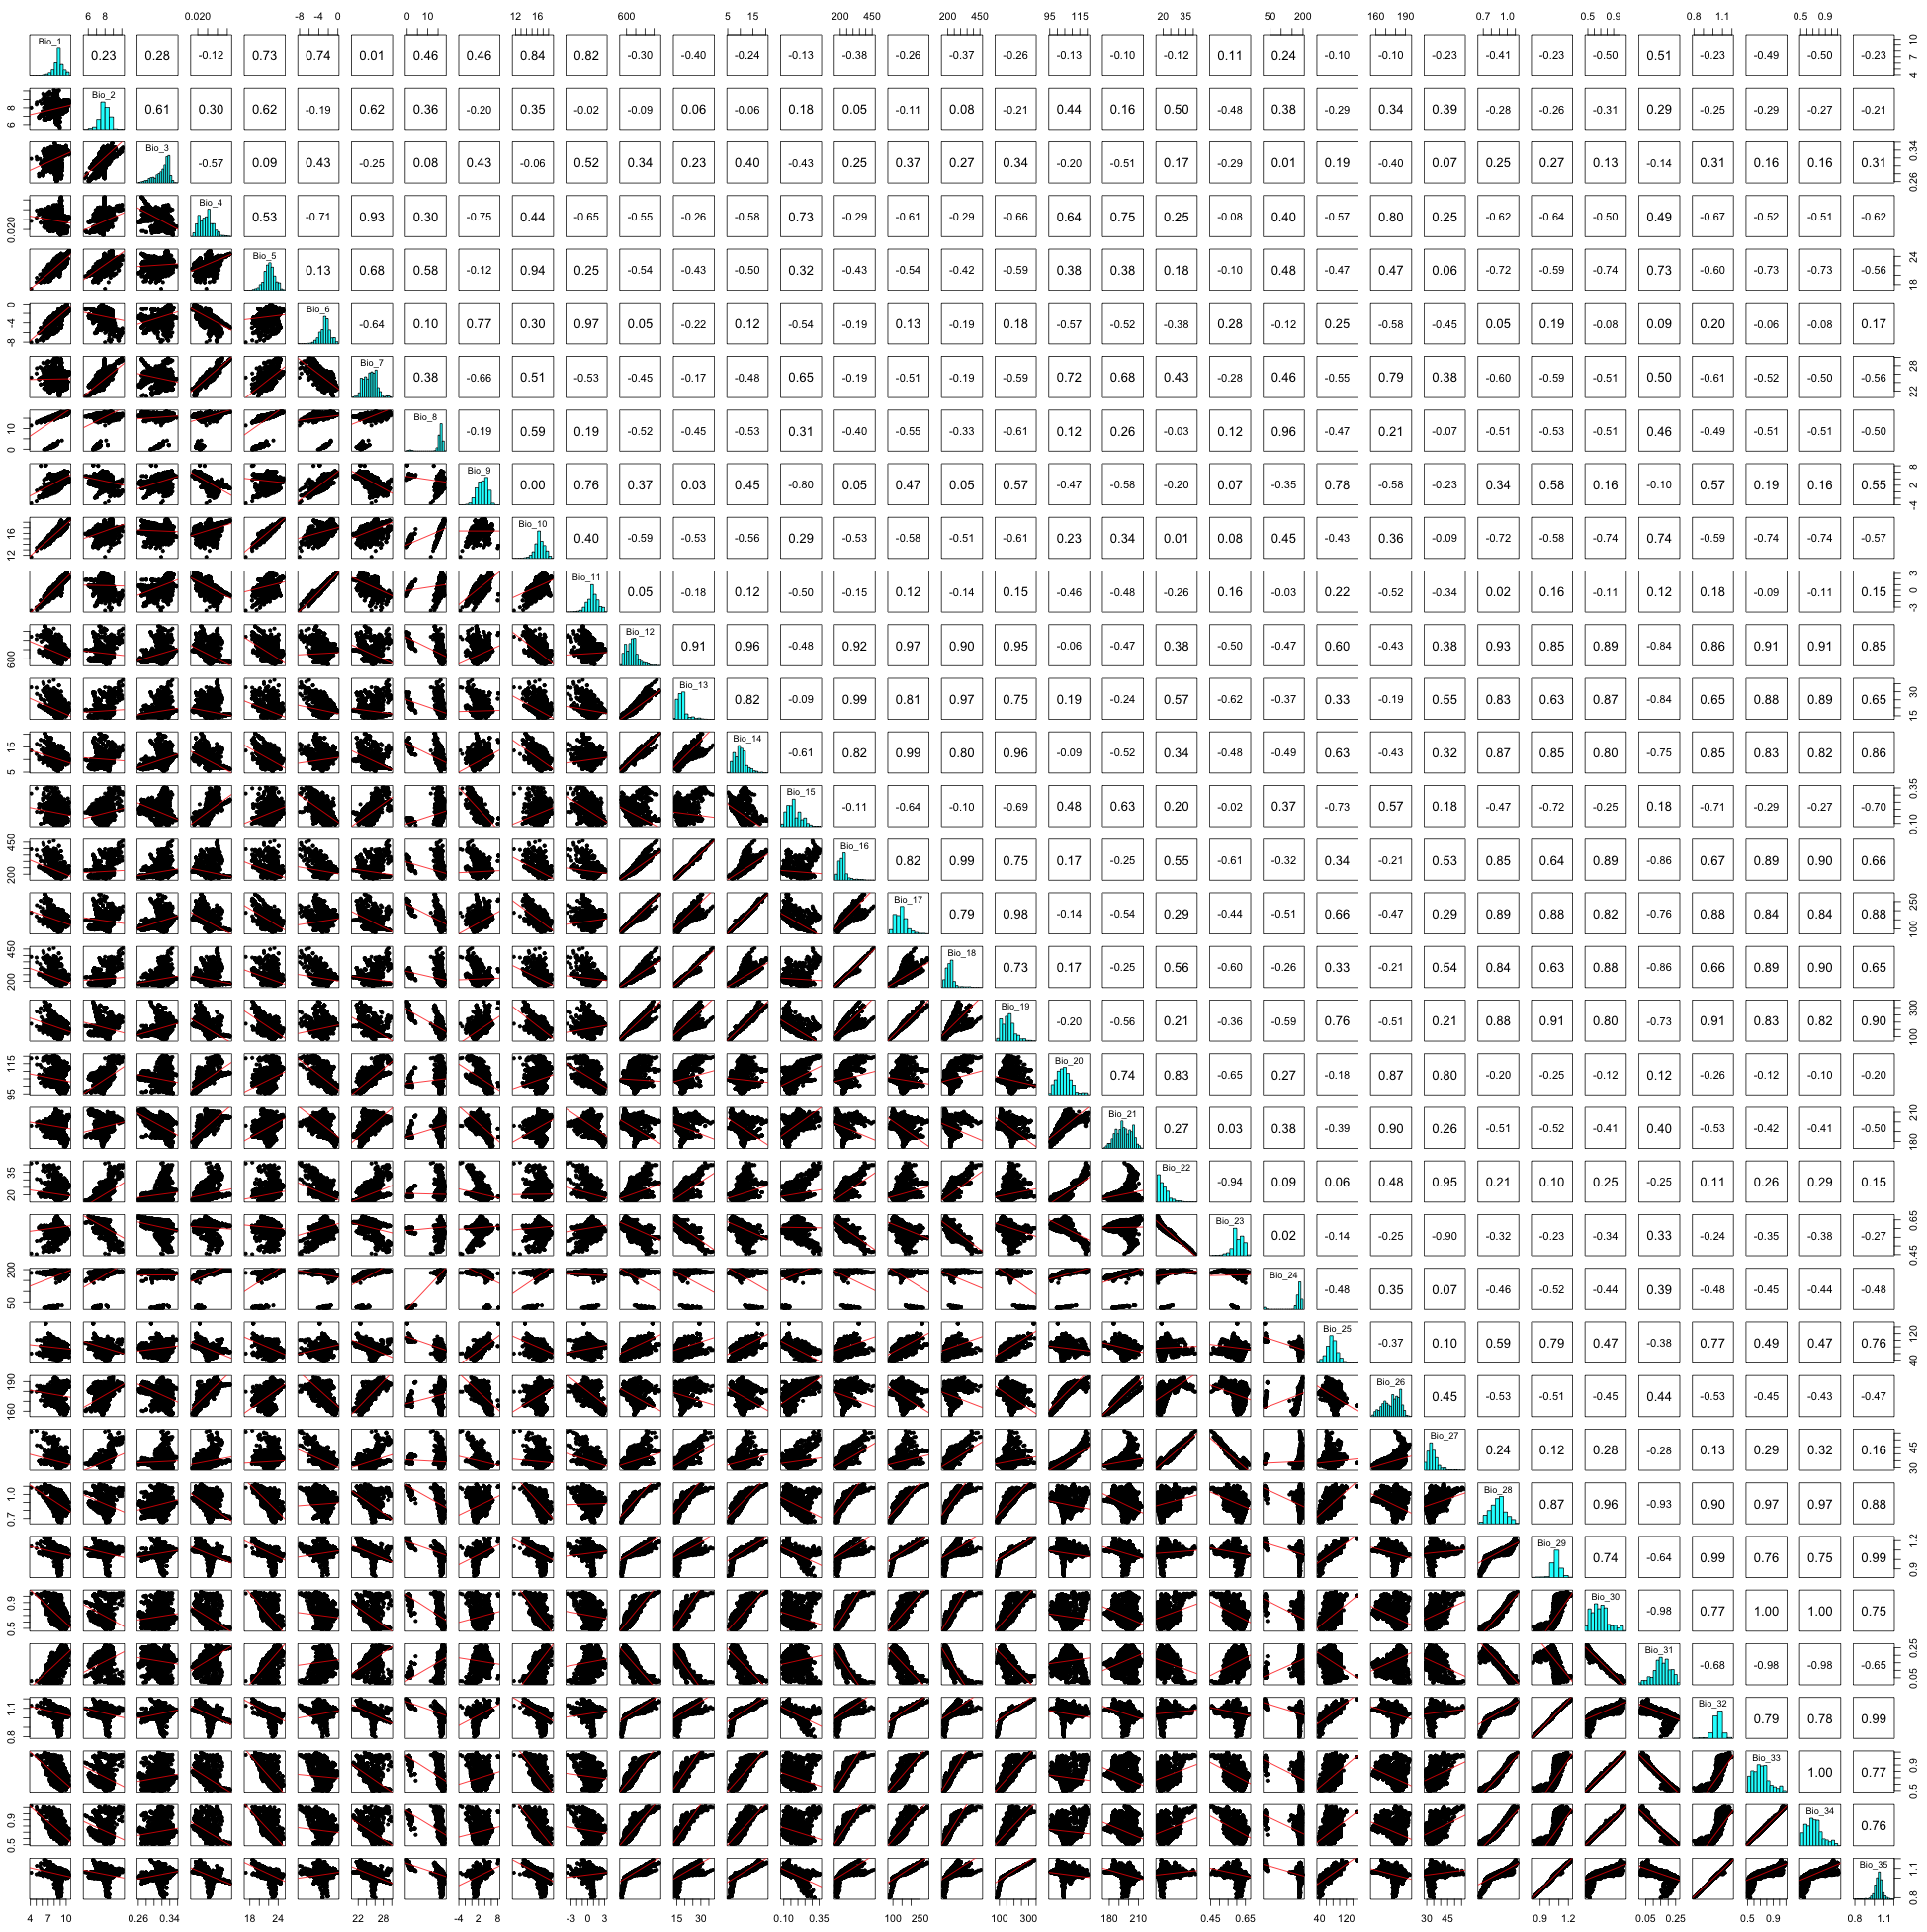
\includegraphics[width=1.2\textwidth]{Figures/Fig_C_5.png}
  \caption{Observed multicollinearity among the 35 bioclimatic indices (BIs). Statistically significant (p<0.001) pairwise correlation coefficients (Pearson) are reported with scatterplots and histograms showing distribution. Details on the indices and their IDs and units can be found in Table 2 and \href{https://www.climond.org/Resources.aspx}{https://www.climond.org/Resources.aspx}.}
  \label{Fig_C_5}
\end{figure}

\end{landscape}

\clearpage

\begin{figure}[h!]
  \centering
  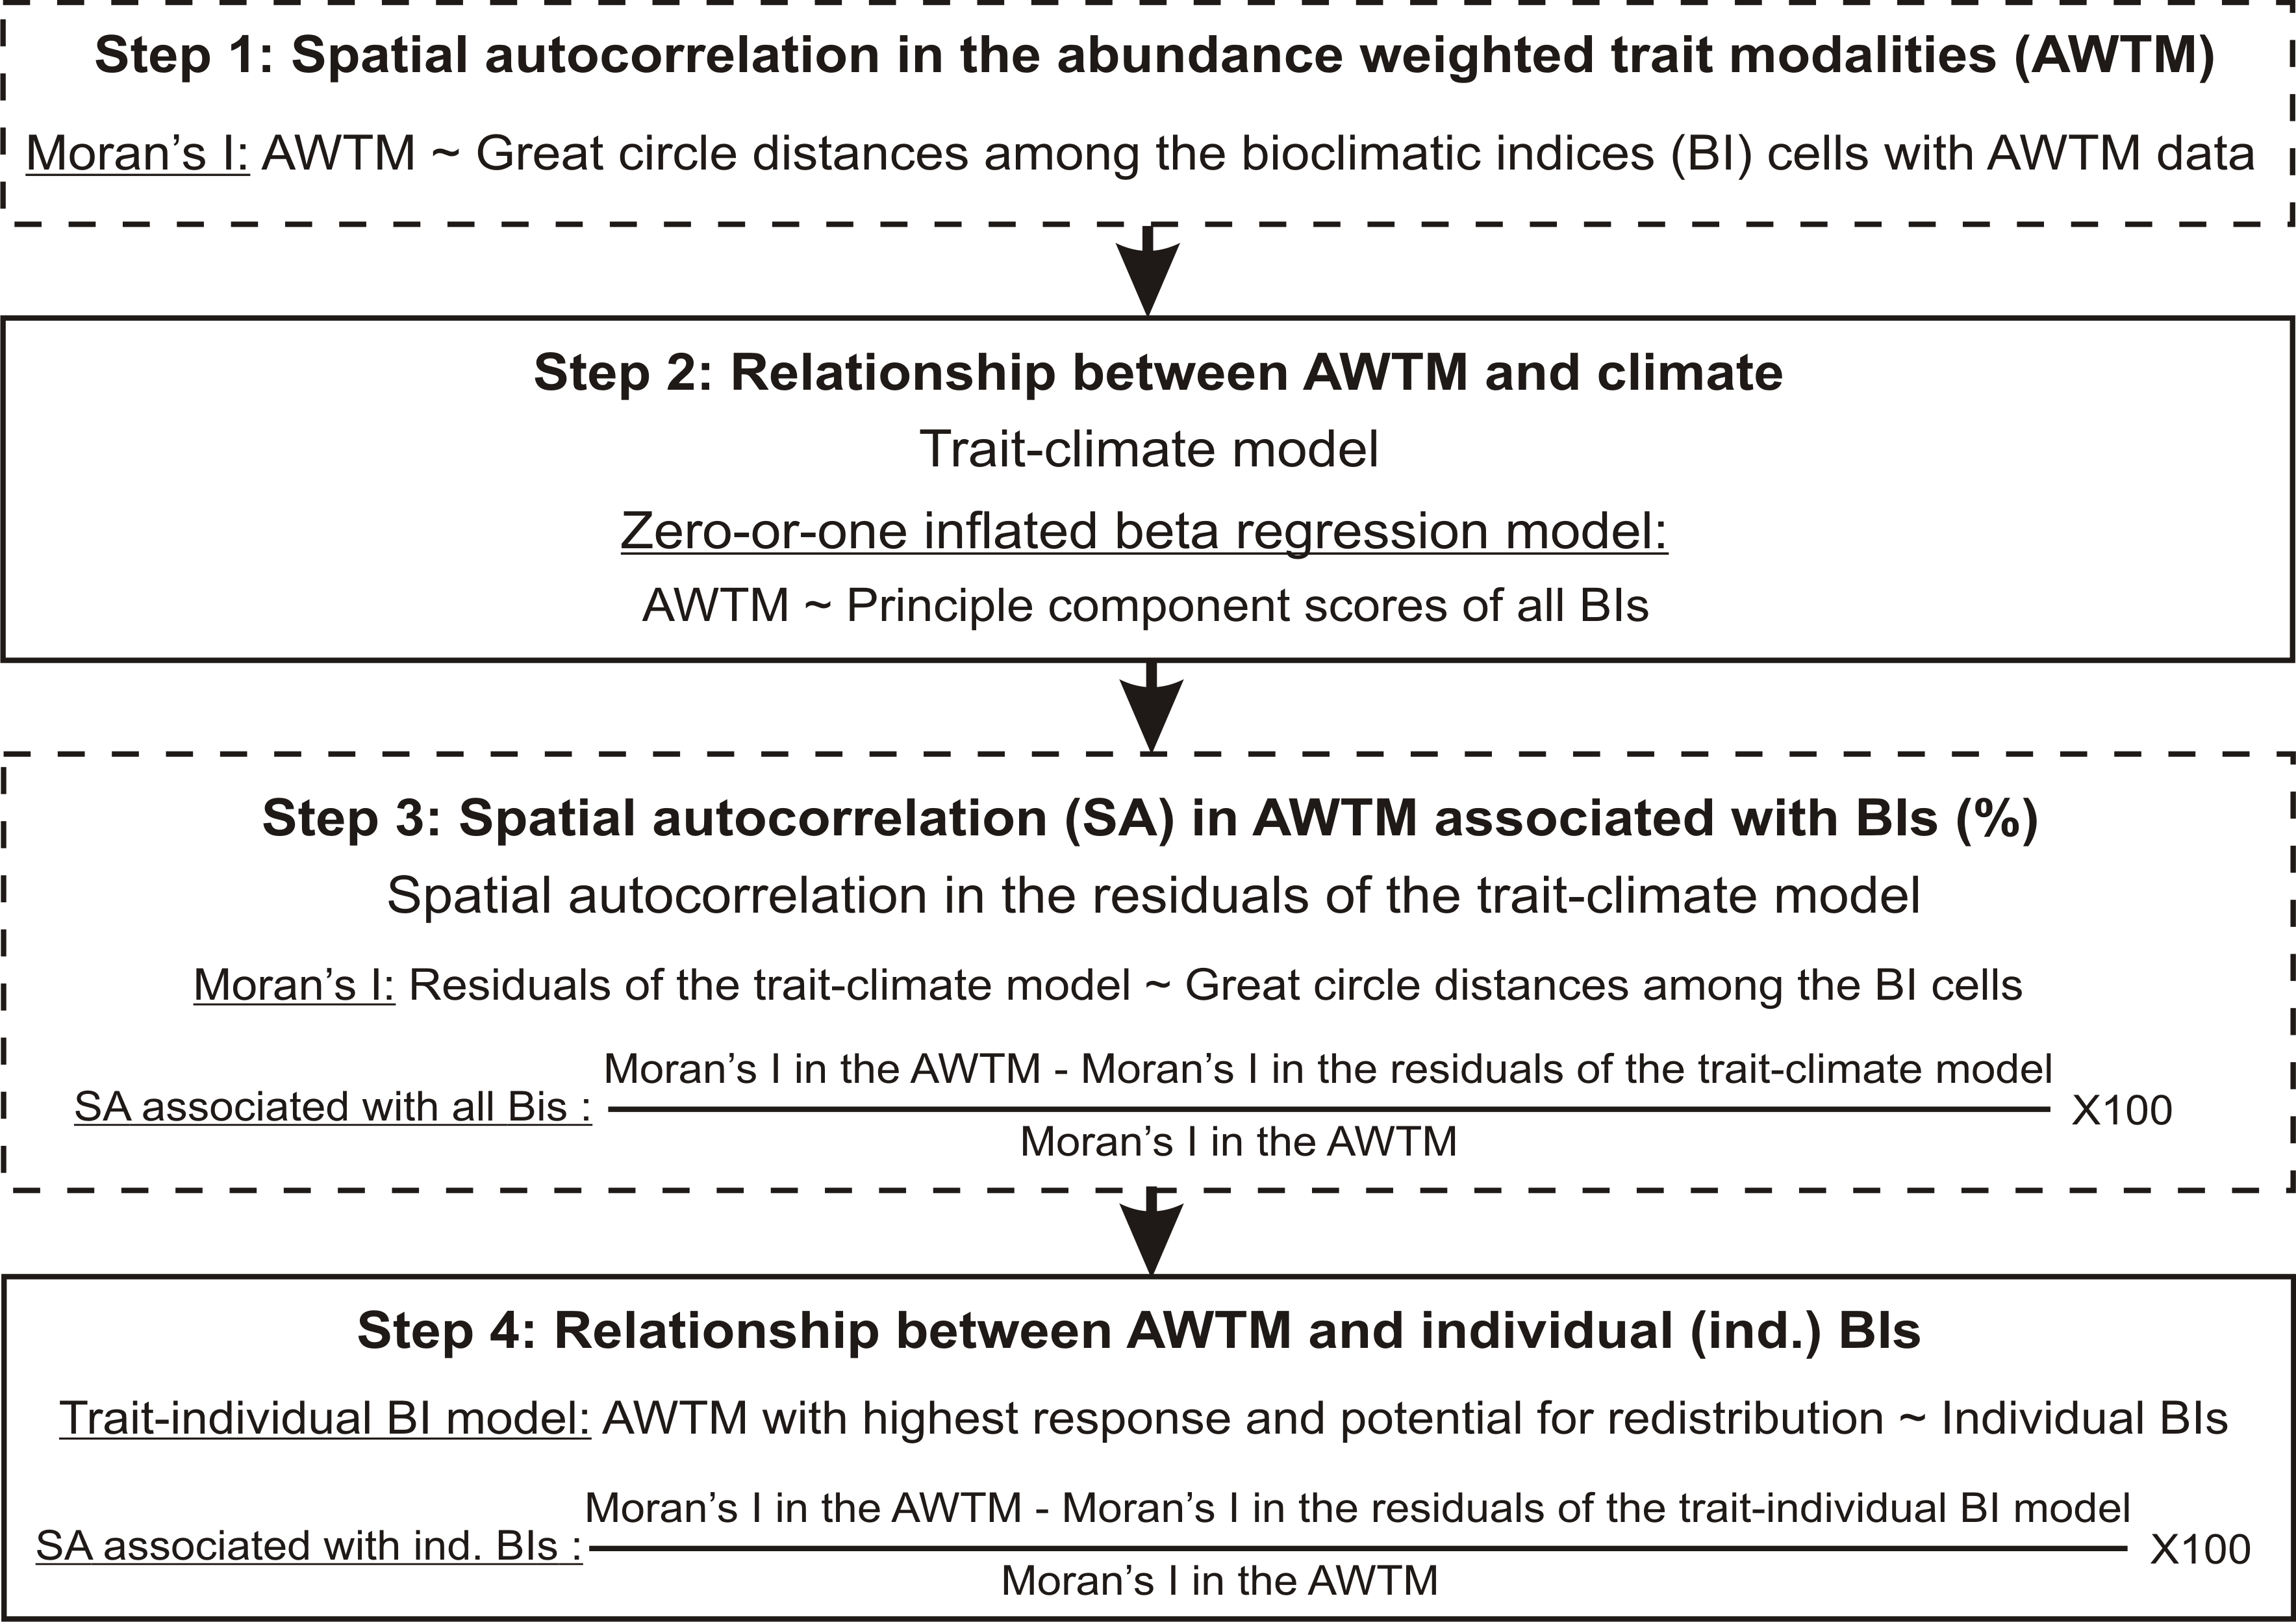
\includegraphics[width=1.1\textwidth]{Figures/Fig_C_6.png}
  \caption{Steps of the trait-climate spatial relationship analysis.}
  \label{Fig_C_6}
\end{figure}

\clearpage

\section{Supplementary tables}
\label{Supplementary tables}

\setlength{\LTcapwidth}{\linewidth}

\begin{longtable}[c]{>{\centering\arraybackslash}m{3.6cm}>{\centering\arraybackslash}m{1.3cm}>{\centering\arraybackslash}m{2.0cm}>{\centering\arraybackslash}m{1.3cm}>{\centering\arraybackslash}m{1.5cm}>{\centering\arraybackslash}m{1.5cm}}

\caption{Membership states of the five insect orders (\%) for the traits of each grouping feature. The membership state (\%) of an order for a trait was computed as the median of the membership states of all taxa in that order for that trait. The membership states were then scaled by the total of the membership states of an order for the traits of a grouping feature so that the membership states sum to 100 \% for each grouping feature.}

\centering

\hline
\textbf{Grouping features and traits} & \multicolumn{5}{c}{\textbf{Aquatic insect orders}}\\
 & \textbf{Diptera} & \textbf{Ephemeroptera} & \textbf{Odonata} & \textbf{Plecoptera} & \textbf{Trichoptera}\\
\hline
\endfirsthead

\hline
\endhead

\hline
\endfoot

\hline
\endlastfoot

\textbf{Biological traits} & & & & & \\
\textit{Dispersal capacity} & & & & & \\
Unknown & NA & NA & NA & NA & 9\\
Low & NA & 100* & NA & 100* & 36\\
High & NA & NA & NA & NA & 55*\\
\textit{Maximal body size} & & & & & \\
> 0.25 cm to 0.5 cm & 11 & 3 & NA & 6 & 11\\
> 0.5 cm to 1 cm & 39* & 43 & 3 & 39* & 37\\
> 1 cm to 2 cm & 29 & 50* & 44* & 36 & 39*\\
> 2 cm to 4 cm & 14 & 3 & 44* & 19 & 13\\
> 4 cm to 8 cm & 7 & NA & 9 & NA & NA\\
\textit{Reproductive capacity} & & & & & \\
Flexible & NA & 4 & NA & 7 & 5\\
Semivoltine & 4 & 2 & NA & 15 & 10\\
Univoltine & 39 & 64* & NA & 79* & 80*\\
Bivoltine & 44* & 23 & NA & NA & 4\\
Trivoltine & 11 & 5 & NA & NA & NA\\
Multivoltine & 3 & 1 & NA & NA & 1\\
\textit{Resistance to drought} & & & & & \\
Unknown resistance type & NA & NA & NA & 28 & 4\\
No drought resilience & NA & NA & NA & NA & 49*\\
Egg diapause & NA & 60* & NA & 62* & 3\\
Larvae diapause & NA & 40 & NA & 10 & 4\\
Adult diapause & NA & NA & NA & NA & 40\\
\textbf{Ecological traits} & & & & & \\
\textit{Current preference} & & & & & \\
Indifferent & 13 & NA & NA & 3 & 3\\
Limnobiont & 7 & 1 & 21 & NA & 19\\
Limnophil & 17 & 11 & 49* & 1 & 16\\
Limno to Rheophil & 4 & 10 & 14 & 2 & 12\\
Rheo to Limnophil & 14 & 27 & 7 & 10 & 13\\
Rheophil & 31* & 45* & 7 & 80* & 26*\\
Rheobiont & 13 & 7 & 3 & 5 & 11\\
\textit{Temperature preference} & & & & & \\
Eurytherm & 30* & 7 & NA & 1 & 48*\\
Very cold & 3 & 15 & NA & 16 & 6\\
Cold & 14 & 27 & NA & 46* & 14\\
Moderate & 26 & 32* & NA & 27 & 23\\
Warm & 27 & 19 & NA & 10 & 10\\

\end{longtable}

\vspace{-0.45cm}

\footnotesize
\textsuperscript{NA}Trait not occurring, *The highest membership state (\%) of an insect order for a trait in a grouping feature

\normalsize

\newpage

\begin{table}[hp!]

\label{Table C.2}

\caption{Spatial autocorrelations (Moran's I values) and gradients (Pearson correlations with longitude, latitude and altitude) for the bioclimatic indices (BIs) extracted at the stream sites. The Moran's I values and Pearson correlation coefficients are statistically significant at p<0.001. Details on the indices and their IDs and units can be found in Table 2 and \href{https://www.climond.org/Resources.aspx}{https://www.climond.org/Resources.aspx}.}

\centering

\begin{tabular}{>{\centering\arraybackslash}m{2.0cm}>{\centering\arraybackslash}m{2.0cm}>{\centering\arraybackslash}m{1.5cm}>{\centering\arraybackslash}m{1.5cm}>{\centering\arraybackslash}m{1.0cm}}

\toprule
\textbf{Bioclimatic indices} & \textbf{Spatial autocorrelation} & \multicolumn{3}{c}{\textbf{Correlation (Pearson) with spatial variables}}\\
\textbf{(BIs)} & \textbf{(Global Moran's I)} & & & \\
 & & \textbf{Longitude} & \textbf{Latitude} & \textbf{Altitude}\\

\midrule

Bio01 & 0.18 & -0.42 & 0.30 & -0.77\\
Bio02 & 0.29 & 0.16 & -0.77 & 0.52\\
Bio03 & 0.28 & -0.54 & -0.53 & 0.26\\
Bio04 & 0.36 & 0.86 & -0.34 & 0.30\\
Bio05 & 0.13 & 0.10 & -0.20 & -0.32\\
Bio06 & 0.32 & -0.68 & 0.49 & -0.76\\
Bio07 & 0.34 & 0.68 & -0.58 & 0.45\\
Bio08 & 0.09 & 0.28 & 0.13 & -0.3\\
Bio09 & 0.30 & -0.75 & 0.33 & -0.58\\
Bio10 & 0.12 & 0.00 & 0.15 & -0.64\\
Bio11 & 0.30 & -0.70 & 0.40 & -0.73\\
Bio12 & 0.27 & -0.27 & -0.58 & 0.69\\
Bio13 & 0.30 & 0.04 & -0.67 & 0.80\\
Bio14 & 0.26 & -0.45 & -0.55 & 0.60\\
Bio15 & 0.30 & 0.72 & -0.28 & 0.33\\
Bio16 & 0.30 & 0.03 & -0.66 & 0.79\\
Bio17 & 0.25 & -0.44 & -0.51 & 0.59\\
Bio18 & 0.30 & 0.05 & -0.66 & 0.79\\
Bio19 & 0.24 & -0.53 & -0.39 & 0.47\\
Bio20 & 0.38 & 0.36 & -0.78 & 0.68\\
Bio21 & 0.29 & 0.43 & -0.23 & 0.11\\
Bio22 & 0.40 & 0.16 & -0.89 & 0.84\\
Bio23 & 0.41 & -0.09 & 0.92 & -0.86\\
Bio24 & 0.13 & 0.43 & -0.14 & 0.08\\
Bio25 & 0.20 & -0.53 & 0.02 & 0.04\\
Bio26 & 0.33 & 0.53 & -0.51 & 0.35\\
Bio27 & 0.37 & 0.25 & -0.78 & 0.83\\
Bio28 & 0.24 & -0.33 & -0.37 & 0.56\\
Bio29 & 0.19 & -0.48 & -0.13 & 0.29\\
Bio30 & 0.25 & -0.09 & -0.46 & 0.67\\
Bio31 & 0.26 & 0.06 & 0.47 & -0.64\\
Bio32 & 0.20 & -0.51 & -0.16 & 0.31\\
Bio33 & 0.25 & -0.14 & -0.47 & 0.66\\
Bio34 & 0.25 & -0.12 & -0.48 & 0.69\\
Bio35 & 0.20 & -0.51 & -0.21 & 0.30\\

\bottomrule

\end{tabular}
\end{table}

\newpage

\setlength{\LTcapwidth}{\linewidth}

\begin{longtable}[c]{>{\centering\arraybackslash}m{3.6cm}>{\centering\arraybackslash}m{1.0cm}>{\centering\arraybackslash}m{2.0cm}>{\centering\arraybackslash}m{1.0cm}>{\centering\arraybackslash}m{1.2cm}>{\centering\arraybackslash}m{1.2cm}>{\centering\arraybackslash}m{1.2cm}}

\caption{Spatial autocorrelations (global Moran's I) for abundance weighted traits in each stream macroinvertebrate order and in the full data. Observed Moran's I values are statistically significant at p<0.001.}

\centering

\hline
\textbf{Grouping features and traits} & \multicolumn{5}{c}{\textbf{Aquatic insect orders}} & \textbf{Full data}\\
 & \textbf{Diptera} & \textbf{Ephemeroptera} & \textbf{Odonata} & \textbf{Plecoptera} & \textbf{Trichoptera} & \\
\hline
\endfirsthead

\hline
\endhead

\hline
\endfoot

\hline
\textbf{\textit{Average over traits and orders}} & \textbf{\textit{0.06}} & \textbf{\textit{0.06}} & \textbf{\textit{0.07}} & \textbf{\textit{0.09}} & \textbf{\textit{0.05}} & \textbf{\textit{0.06}}\\
\hline
\endlastfoot

\textbf{Biological traits} & & & & & & \\
\textit{Dispersal capacity} & & & & & & \\
Unknown & NA & NA & NA & NA & 0.05 & 0.03\\
Low & NA & * & NA & * & 0.03 & 0.04\\
High & NA & NA & NA & NA & 0.02 & 0.03\\
\textit{Average} & \textit{NA} & \textit{NA} & \textit{NA} & \textit{NA} & \textit{0.03} & \textit{0.03}\\
\textit{Maximal body size} & & & & & & \\
> 0.25 cm to 0.5 cm & 0.02 & 0.04 & NA & 0.12 & 0.03 & 0.04\\
> 0.5 cm to 1 cm & 0.03 & 0.02 & NA & 0.03 & 0.03 & 0.03\\
> 1 cm to 2 cm & 0.02 & 0.04 & 0.13 & 0.15 & 0.03 & 0.03\\
> 2 cm to 4 cm & 0.04 & 0.03 & 0.06 & 0.04 & 0.03 & 0.03\\
> 4 cm to 8 cm & 0.02 & NA & 0.08 & NA & NA & 0.04\\
\textit{Average} & \textit{0.03} & \textit{0.03} & \textit{0.09} & \textit{0.09} & \textit{0.03} & \textit{0.03}\\
\textit{Reproductive capacity} & & & & & & \\
Flexible & NA & 0.07 & NA & 0.08 & 0.02 & 0.03\\
Semivoltine & 0.03 & 0.03 & NA & 0.03 & 0.08 & 0.02\\
Univoltine & 0.12 & 0.03 & NA & 0.04 & 0.07 & 0.04\\
Bivoltine & 0.12 & 0.03 & NA & NA & 0.04 & 0.05\\
Trivoltine & 0.06 & 0.10 & NA & NA & NA & 0.04\\
Multivoltine & 0.05 & 0.08 & NA & NA & 0.01 & 0.03\\
\textit{Average} & \textit{0.08} & \textit{0.06} & \textit{NA} & \textit{0.05} & \textit{0.04} & \textit{0.04}\\
\textit{Resistance to drought} & & & & & & \\
Unknown resistance type & NA & NA & NA & 0.19 & 0.02 & 0.03\\
No drought resilience & NA & NA & NA & NA & 0.10 & 0.04\\
Egg diapause & NA & 0.08 & NA & 0.2 & 0.01 & 0.12\\
Larvae diapause & NA & 0.08 & NA & 0.00 & 0.01 & 0.17\\
Adult diapause & NA & NA & NA & NA & 0.13 & 0.02\\
\textit{Average} & \textit{NA} & \textit{0.08} & \textit{NA} & \textit{0.13} & \textit{0.05} & \textit{0.08}\\
\textbf{Ecological traits} & & & & & & \\
\textit{Current preference} & & & & & & \\
Indifferent & 0.10 & NA & NA & 0.03 & 0.02 & 0.08\\
Limnobiont & 0.01 & NA & 0.02 & NA & 0.10 & 0.07\\
Limnophil & 0.05 & 0.13 & 0.08 & 0.17 & 0.16 & 0.14\\
Limno to Rheophil & 0.07 & 0.01 & 0.10 & 0.02 & 0.04 & 0.02\\
Rheo to Limnophil & 0.04 & 0.07 & 0.04 & 0.00 & 0.01 & 0.03\\
Rheophil & 0.09 & 0.05 & 0.11 & 0.20 & 0.11 & 0.13\\
Rheobiont & 0.06 & 0.07 & 0.05 & 0.06 & 0.13 & 0.15\\
\textit{Average} & \textit{0.06} & \textit{0.07} & \textit{0.07} & \textit{0.08} & \textit{0.08} & \textit{0.09}\\
\textit{Temperature preference} & & & & & & \\
Eurytherm & 0.08 & 0.08 & NA & 0.15 & 0.05 & 0.10\\
Very cold & 0.06 & 0.11 & NA & 0.14 & 0.06 & 0.15\\
Cold & 0.08 & 0.03 & NA & 0.10 & 0.07 & 0.13\\
Moderate & 0.03 & 0.09 & NA & 0.08 & 0.01 & 0.01\\
Warm & 0.07 & 0.03 & NA & 0.09 & 0.05 & 0.06\\
\textit{Average} & \textit{0.06} & \textit{0.07} & \textit{NA} & \textit{0.11} & \textit{0.05} & \textit{0.09}\\

\end{longtable}

\vspace{-0.4cm}

\footnotesize
\textsuperscript{NA}Trait not occurring\\
\hspace{0.4cm} *Trait omitted from the analysis because of zero variability (i.e. all taxa have same trait) and therefore the abundance weighted trait cannot be computed\\

\normalsize

\clearpage

\begin{table}[hp!]

\label{Table C.4}

\caption{Relationship between the traits of temperature preference grouping feature and the traits of remaining grouping features in terms of explained variance (\%). The explained variances are the $R^2$s of the zero-or-one-inflated beta regression models fitted with the abundance weighted traits (AWT) of the temperature preference grouping feature as response and the AWT of the remaining grouping features separately as predictor variables.}

\centering

\begin{threeparttable}

\begin{tabular}{>{\centering\arraybackslash}m{3.6cm}>{\centering\arraybackslash}m{1.3cm}>{\centering\arraybackslash}m{1.4cm}>{\centering\arraybackslash}m{1.0cm}>{\centering\arraybackslash}m{1.3cm}>{\centering\arraybackslash}m{1.0cm}}

\toprule
\textbf{Remaining grouping features and traits} & \multicolumn{5}{c}{\textbf{Traits of temperature preference grouping feature}}\\
 & \textbf{Eurytherm} & \textbf{Very cold} & \textbf{Cold} & \textbf{Moderate} & \textbf{Warm}\\

\midrule

\textbf{Biological traits} & & & & & \\
\textit{Dispersal capacity} & & & & & \\
Unknown & 3.6* & 0.1 & 2.0 & 0.0 & 0.0\\
Low & 3.2 & 1.2* & 9.8* & 1.5* & 15\\
High & 0.9 & 0.5 & 4.5 & 1.4 & 17*\\
\textit{Maximal body size} & & & & & \\
> 0.25 cm to 0.5 cm & 2.0 & 10 & 2.8 & 3.4* & 2.1*\\
> 0.5 cm to 1 cm & 1.9 & 0.0 & 1.8 & 0.4 & 0.6\\
> 1 cm to 2 cm & 4.4 & 10 & 4.3 & 0.2 & 1.7\\
> 2 cm to 4 cm & 5.7* & 0.0 & 2.7 & 1.1 & 0.1\\
> 4 cm to 8 cm & 3.2 & 13* & 5.8* & 0.3 & 1.9\\
\textit{Reproductive capacity} & & & & & \\
Flexible & 1.6 & 3.2 & 1.1 & 9.7 & 3.2\\
Semivoltine & 0.1 & 9.0 & 16* & 1.7 & 16\\
Univoltine & 2.9 & 15* & 7.5 & 4.2 & 6.7\\
Bivoltine & 2.7 & 1.0 & 4.5 & 0.0 & 0.8\\
Trivoltine & 0.7 & 7.0 & 1.3 & 10 & 0.8\\
Multivoltine & 1.7 & 15 & 0.1 & 14* & 36*\\
\textit{Resistance to drought} & & & & & \\
Unknown resistance type & 1.8 & 6.2 & 0.3 & 1.8 & 11\\
No drought resilience & 6.7 & 2.8 & 6.3 & 0.0 & 0.3\\
Egg diapause & 28* & 13 & 30* & 1.4 & 6.6\\
Larvae diapause & 0.0 & 25* & 0.7 & 0.0 & 0.6\\
Adult diapause & 15 & 0.0 & 16 & 3.7* & 14*\\
\textbf{Ecological traits} & & & & & \\
\textit{Current preference} & & & & & \\
Indifferent & 13 & 36 & 30 & 0.9 & 12*\\
Limnobiont & 12 & 14 & 16 & 0.6 & 0.8\\
Limnophil & 18 & 41 & 27 & 1.3* & 4.6\\
Limno to Rheophil & 0.5 & 1.6 & 0.7 & 0.1 & 0.0\\
Rheo to Limnophil & 3.0 & 0.0 & 0.0 & 0.6 & 0.0\\
Rheophil & 26* & 42* & 35* & 0.2 & 2.6\\
Rheobiont & 5.3 & 16 & 12 & 0.8 & 6.6\\

\bottomrule

\end{tabular}
\begin{tablenotes}
\footnotesize
* The highest explained variance in the traits of the temperature preference grouping feature by the traits of the remaining grouping features
\end{tablenotes}
\end{threeparttable}
\end{table} % Include the third content chapter
\chapter{Supplementary materials for:\\Mapping human health risks from exposure to trace metal contamination of drinking water sources in Pakistan}
\label{appendixD}

\section{Supplementary figures}
\label{Supplementary figures}

See next page.

\begin{landscape}

\begin{figure*}[hp!]
  \centering
  \vspace{-2cm} 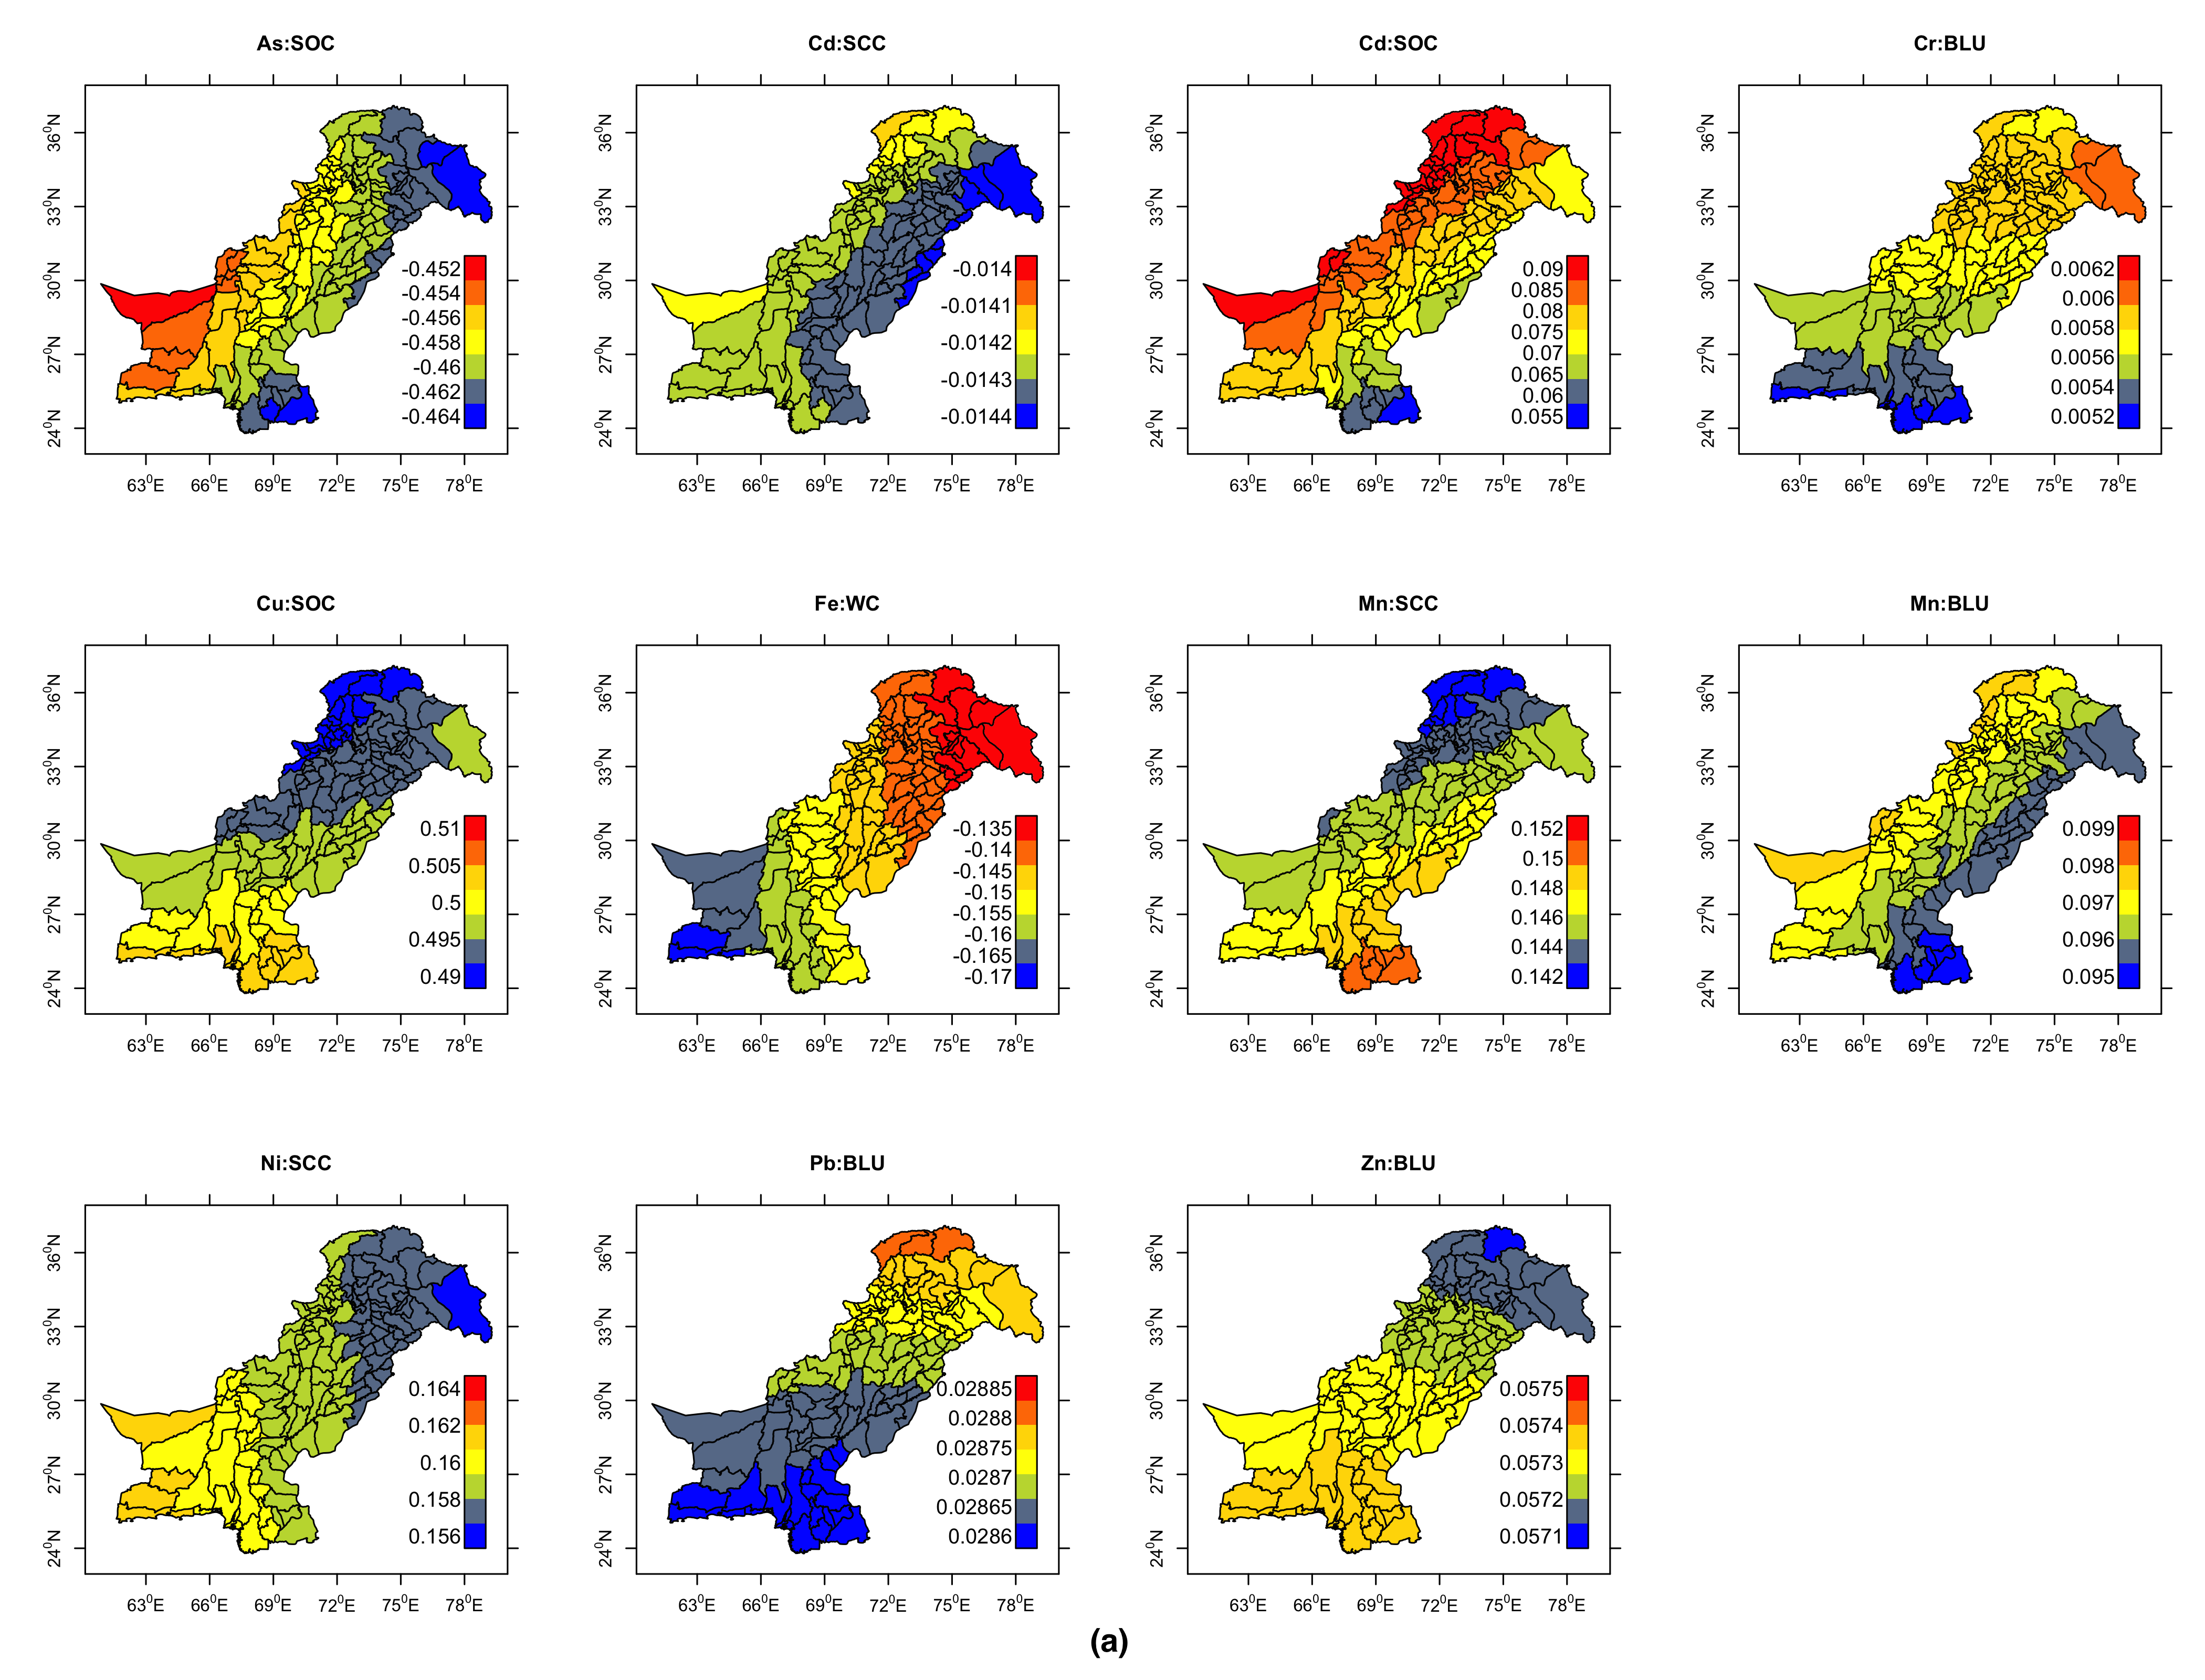
\includegraphics[width=\linewidth]{Figures/Fig_D_1_a.png}
  \label{Fig_D_1_a}
\end{figure*}

\newpage

\begin{figure*}[hp!]
  \centering
  \vspace{-0.5cm} 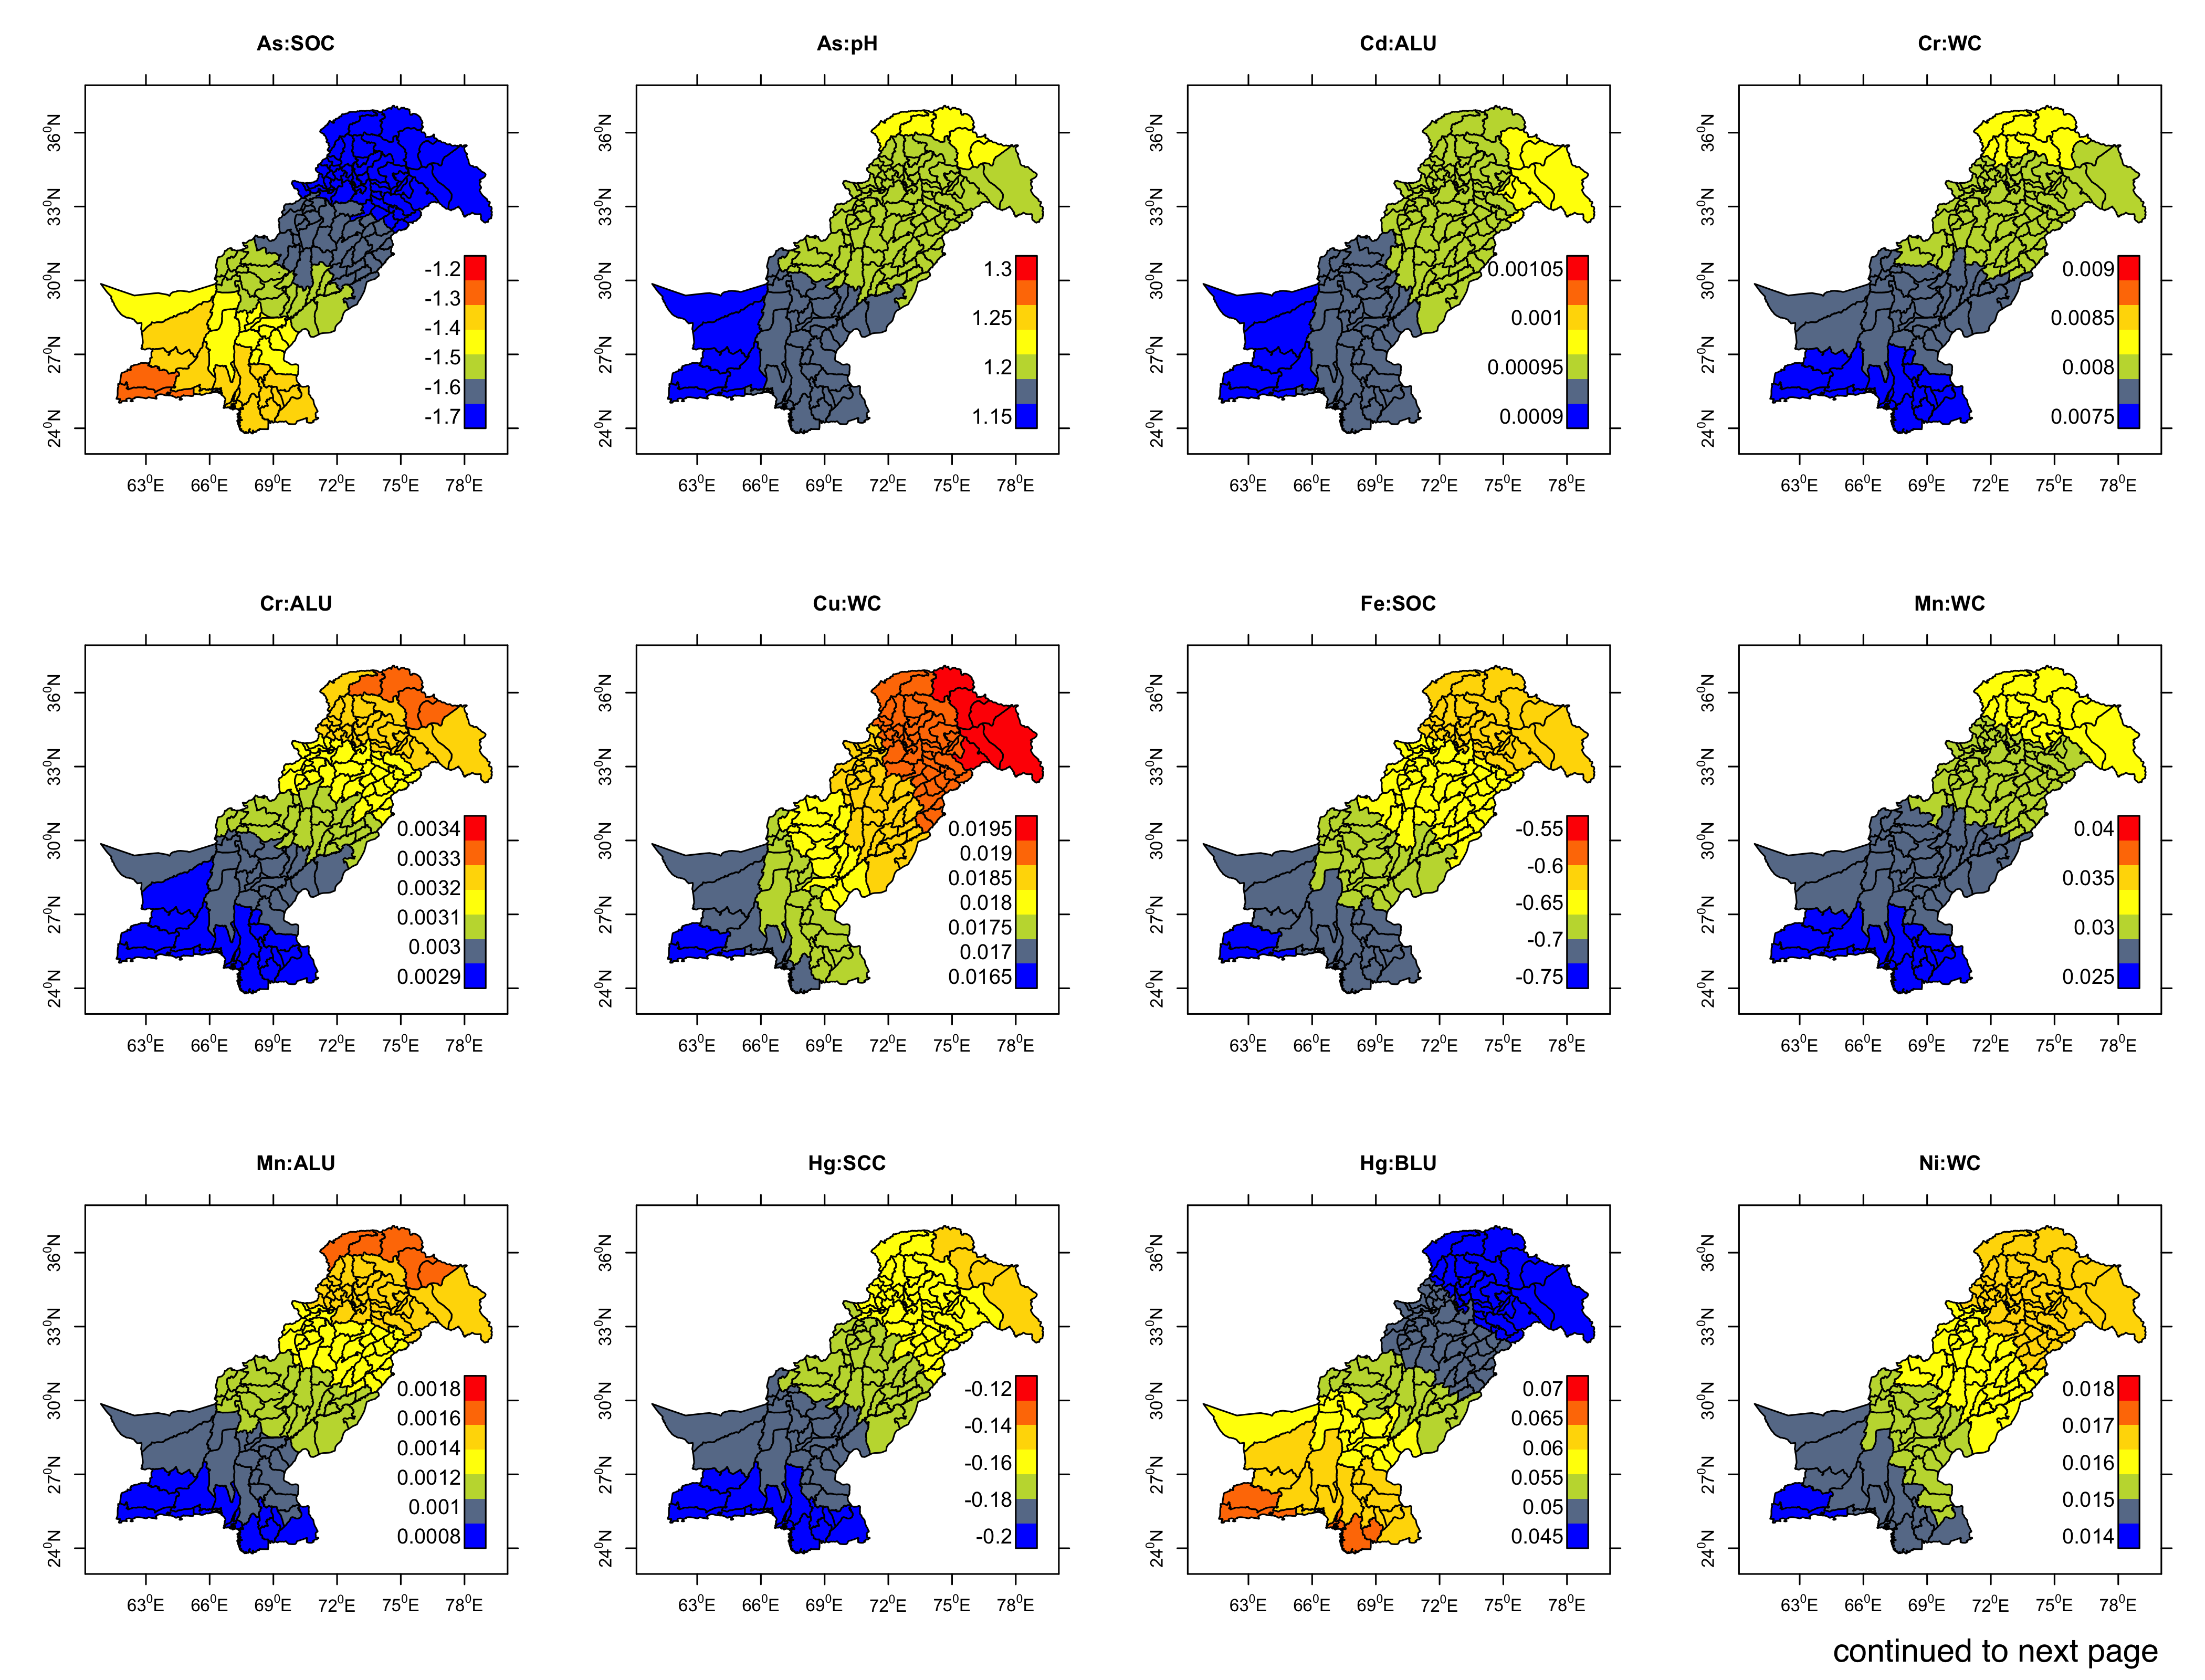
\includegraphics[width=0.95\linewidth]{Figures/Fig_D_1_b_1.png}
  \label{Fig_D_1_b_1}
\end{figure*}

\clearpage

\begin{figure}[h!]
  \centering
  \vspace{-2cm} 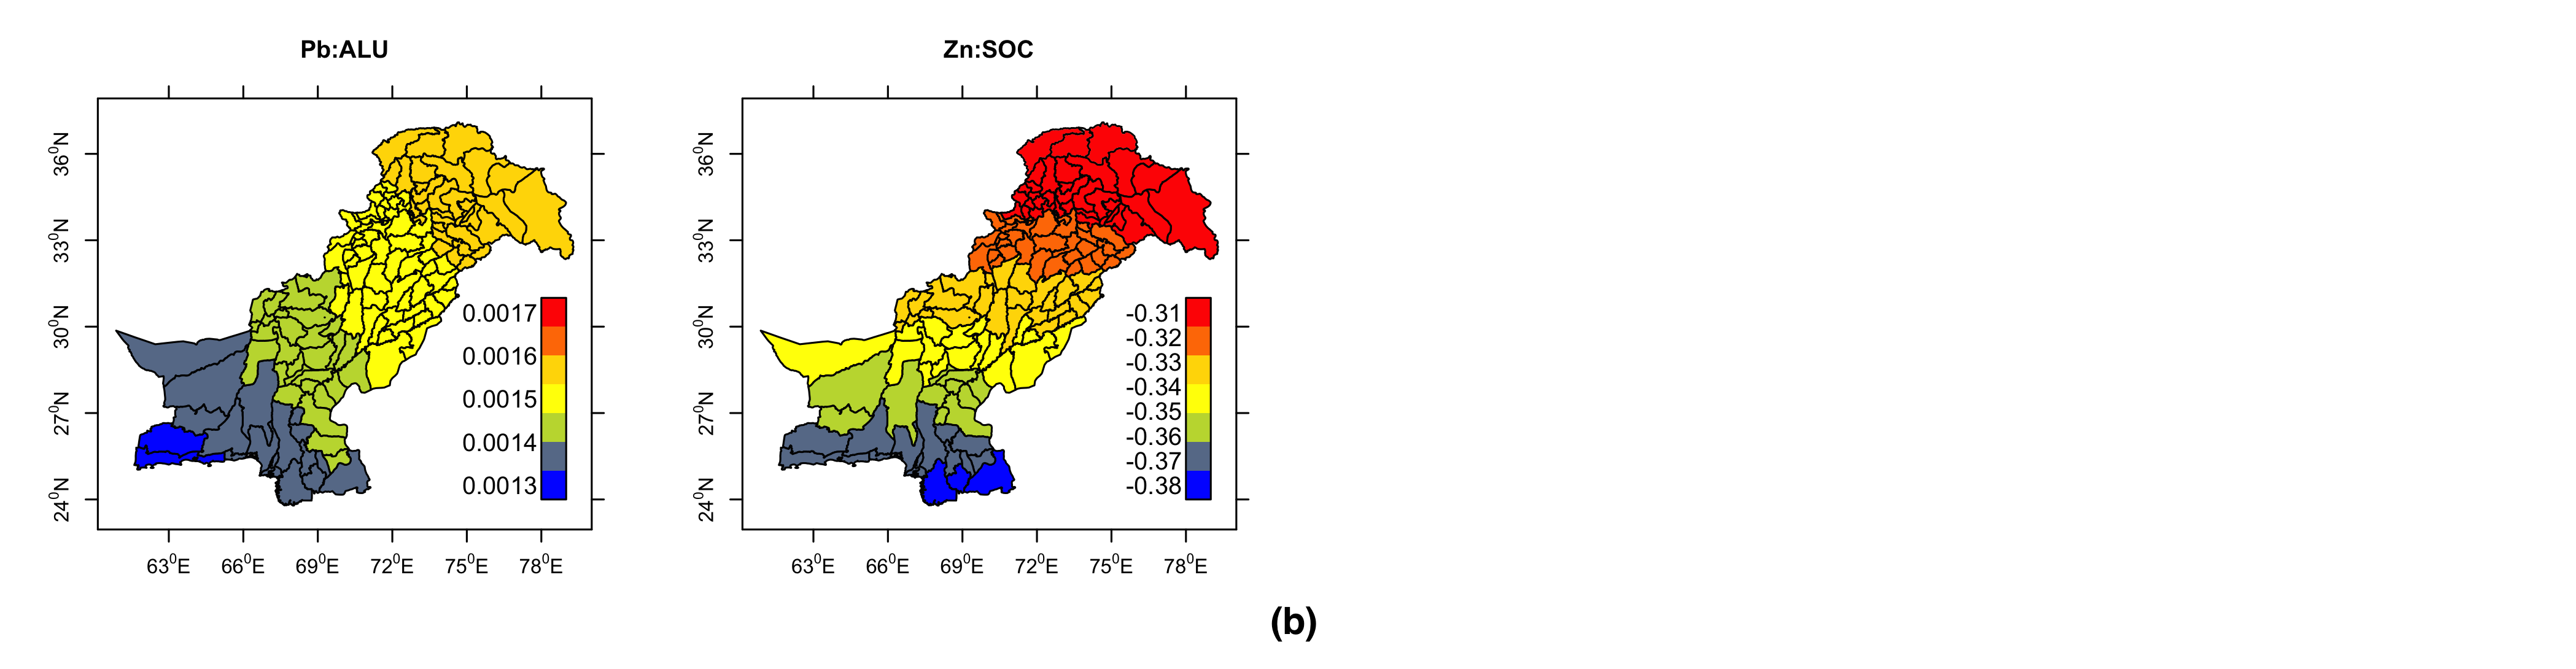
\includegraphics[width=\linewidth]{Figures/Fig_D_1_b_2.png}
  \caption{Geographically weighted regression (GWR) coefficient estimates in each district for the spatial predictors that predicted trace metal concentrations in (a) ground and (b) surface water. The abbreviations used: As = Arsenic, Cd = Cadmium, Cr = Chromium, Cu = Copper, Fe = Iron, Mn = Manganese, Hg = Mercury, Nickel = Ni, Pb = Lead, Zn = Zinc, WC = mean total available water capacity, SOC = mean soil organic carbon density, SCC = mean soil carbonate carbon density, pH= mean soil pH, BLU = percentage of built-up area, ALU = percentage of agricultural area.}
  \label{Fig_D_1_b_2}
\end{figure}

\end{landscape}

\newpage

\begin{figure*}[hp!]
  \centering
  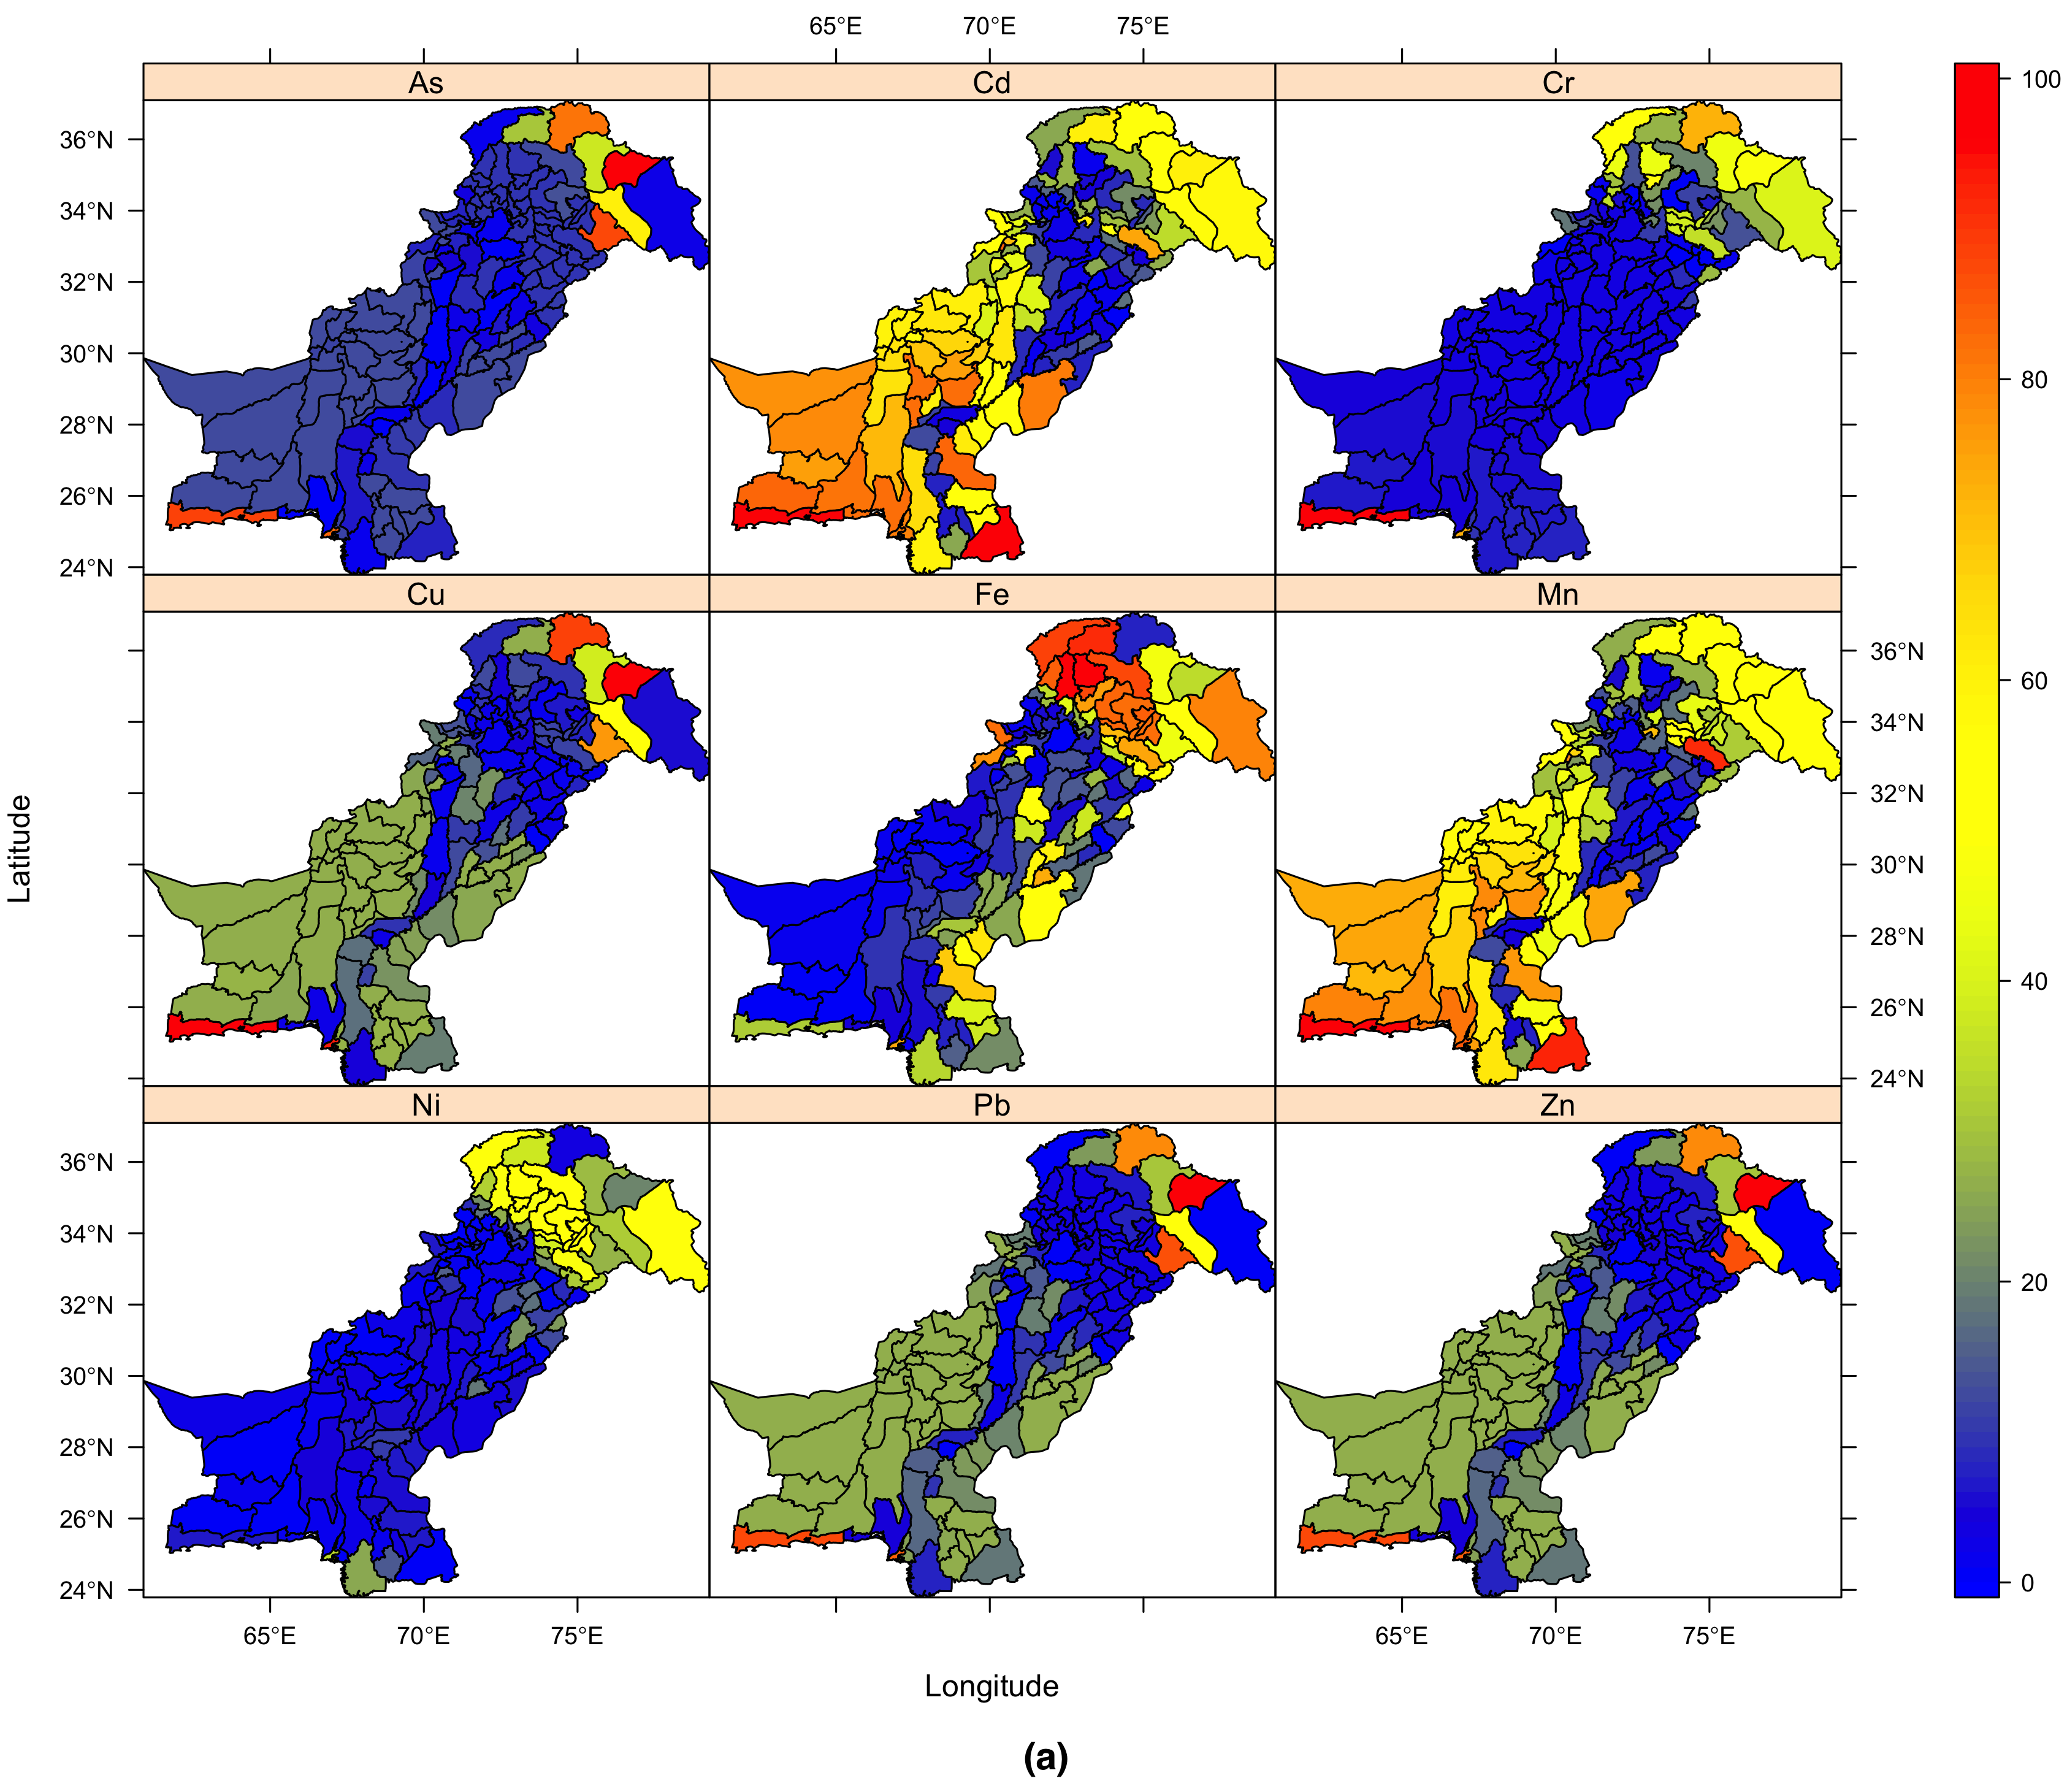
\includegraphics[width=1.1\textwidth]{Figures/Fig_D_2_a.png}
  \label{Fig_D_2_a}
\end{figure*}

\newpage

\begin{landscape}

\begin{figure}[hp!]
  \centering
  \vspace{-2cm} 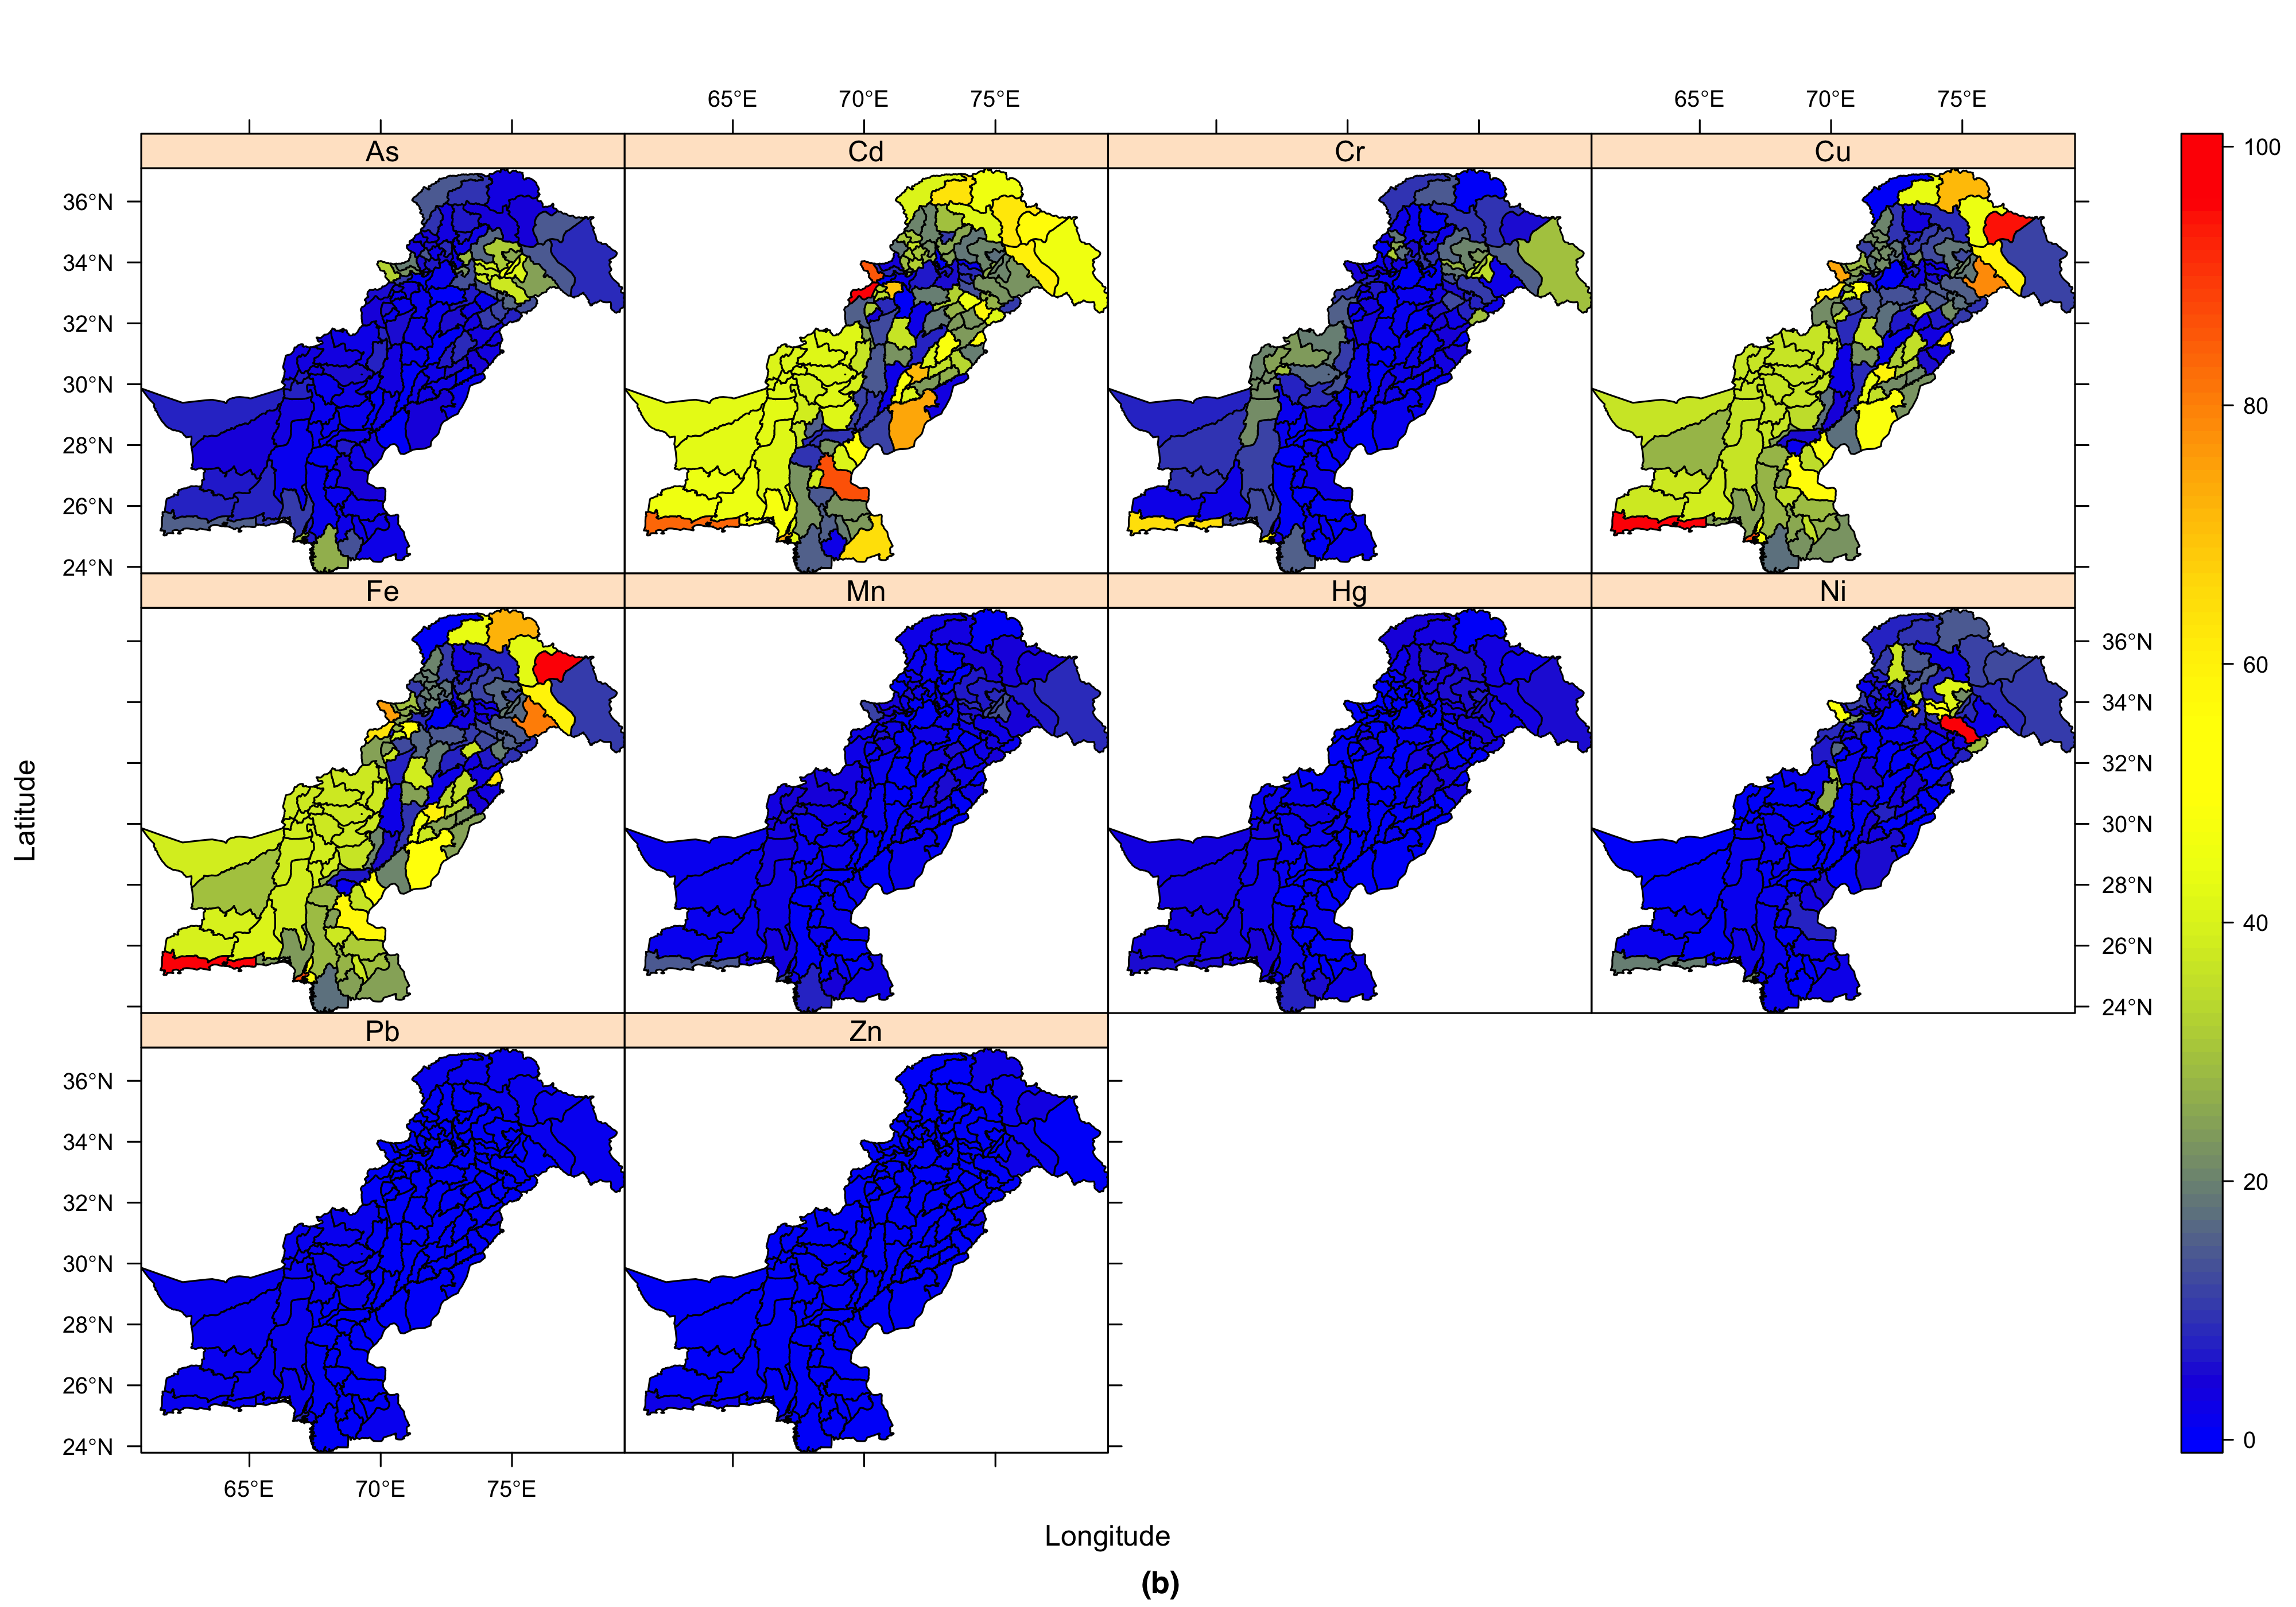
\includegraphics[width=\linewidth]{Figures/Fig_D_2_b.png}
  \caption{GWR prediction standard errors (in \%) for prediction of trace metal concentrations in (a) ground and (b) surface water of each district. The abbreviations used: As = Arsenic, Cd = Cadmium, Cr = Chromium, Cu = Copper, Fe = Iron, Mn = Manganese, Hg = Mercury, Nickel = Ni, Pb = Lead, Zn = Zinc.}
  \label{Fig_D_2_b}
\end{figure}

\end{landscape}

\newpage

\begin{figure*}[hp!]
  \centering
  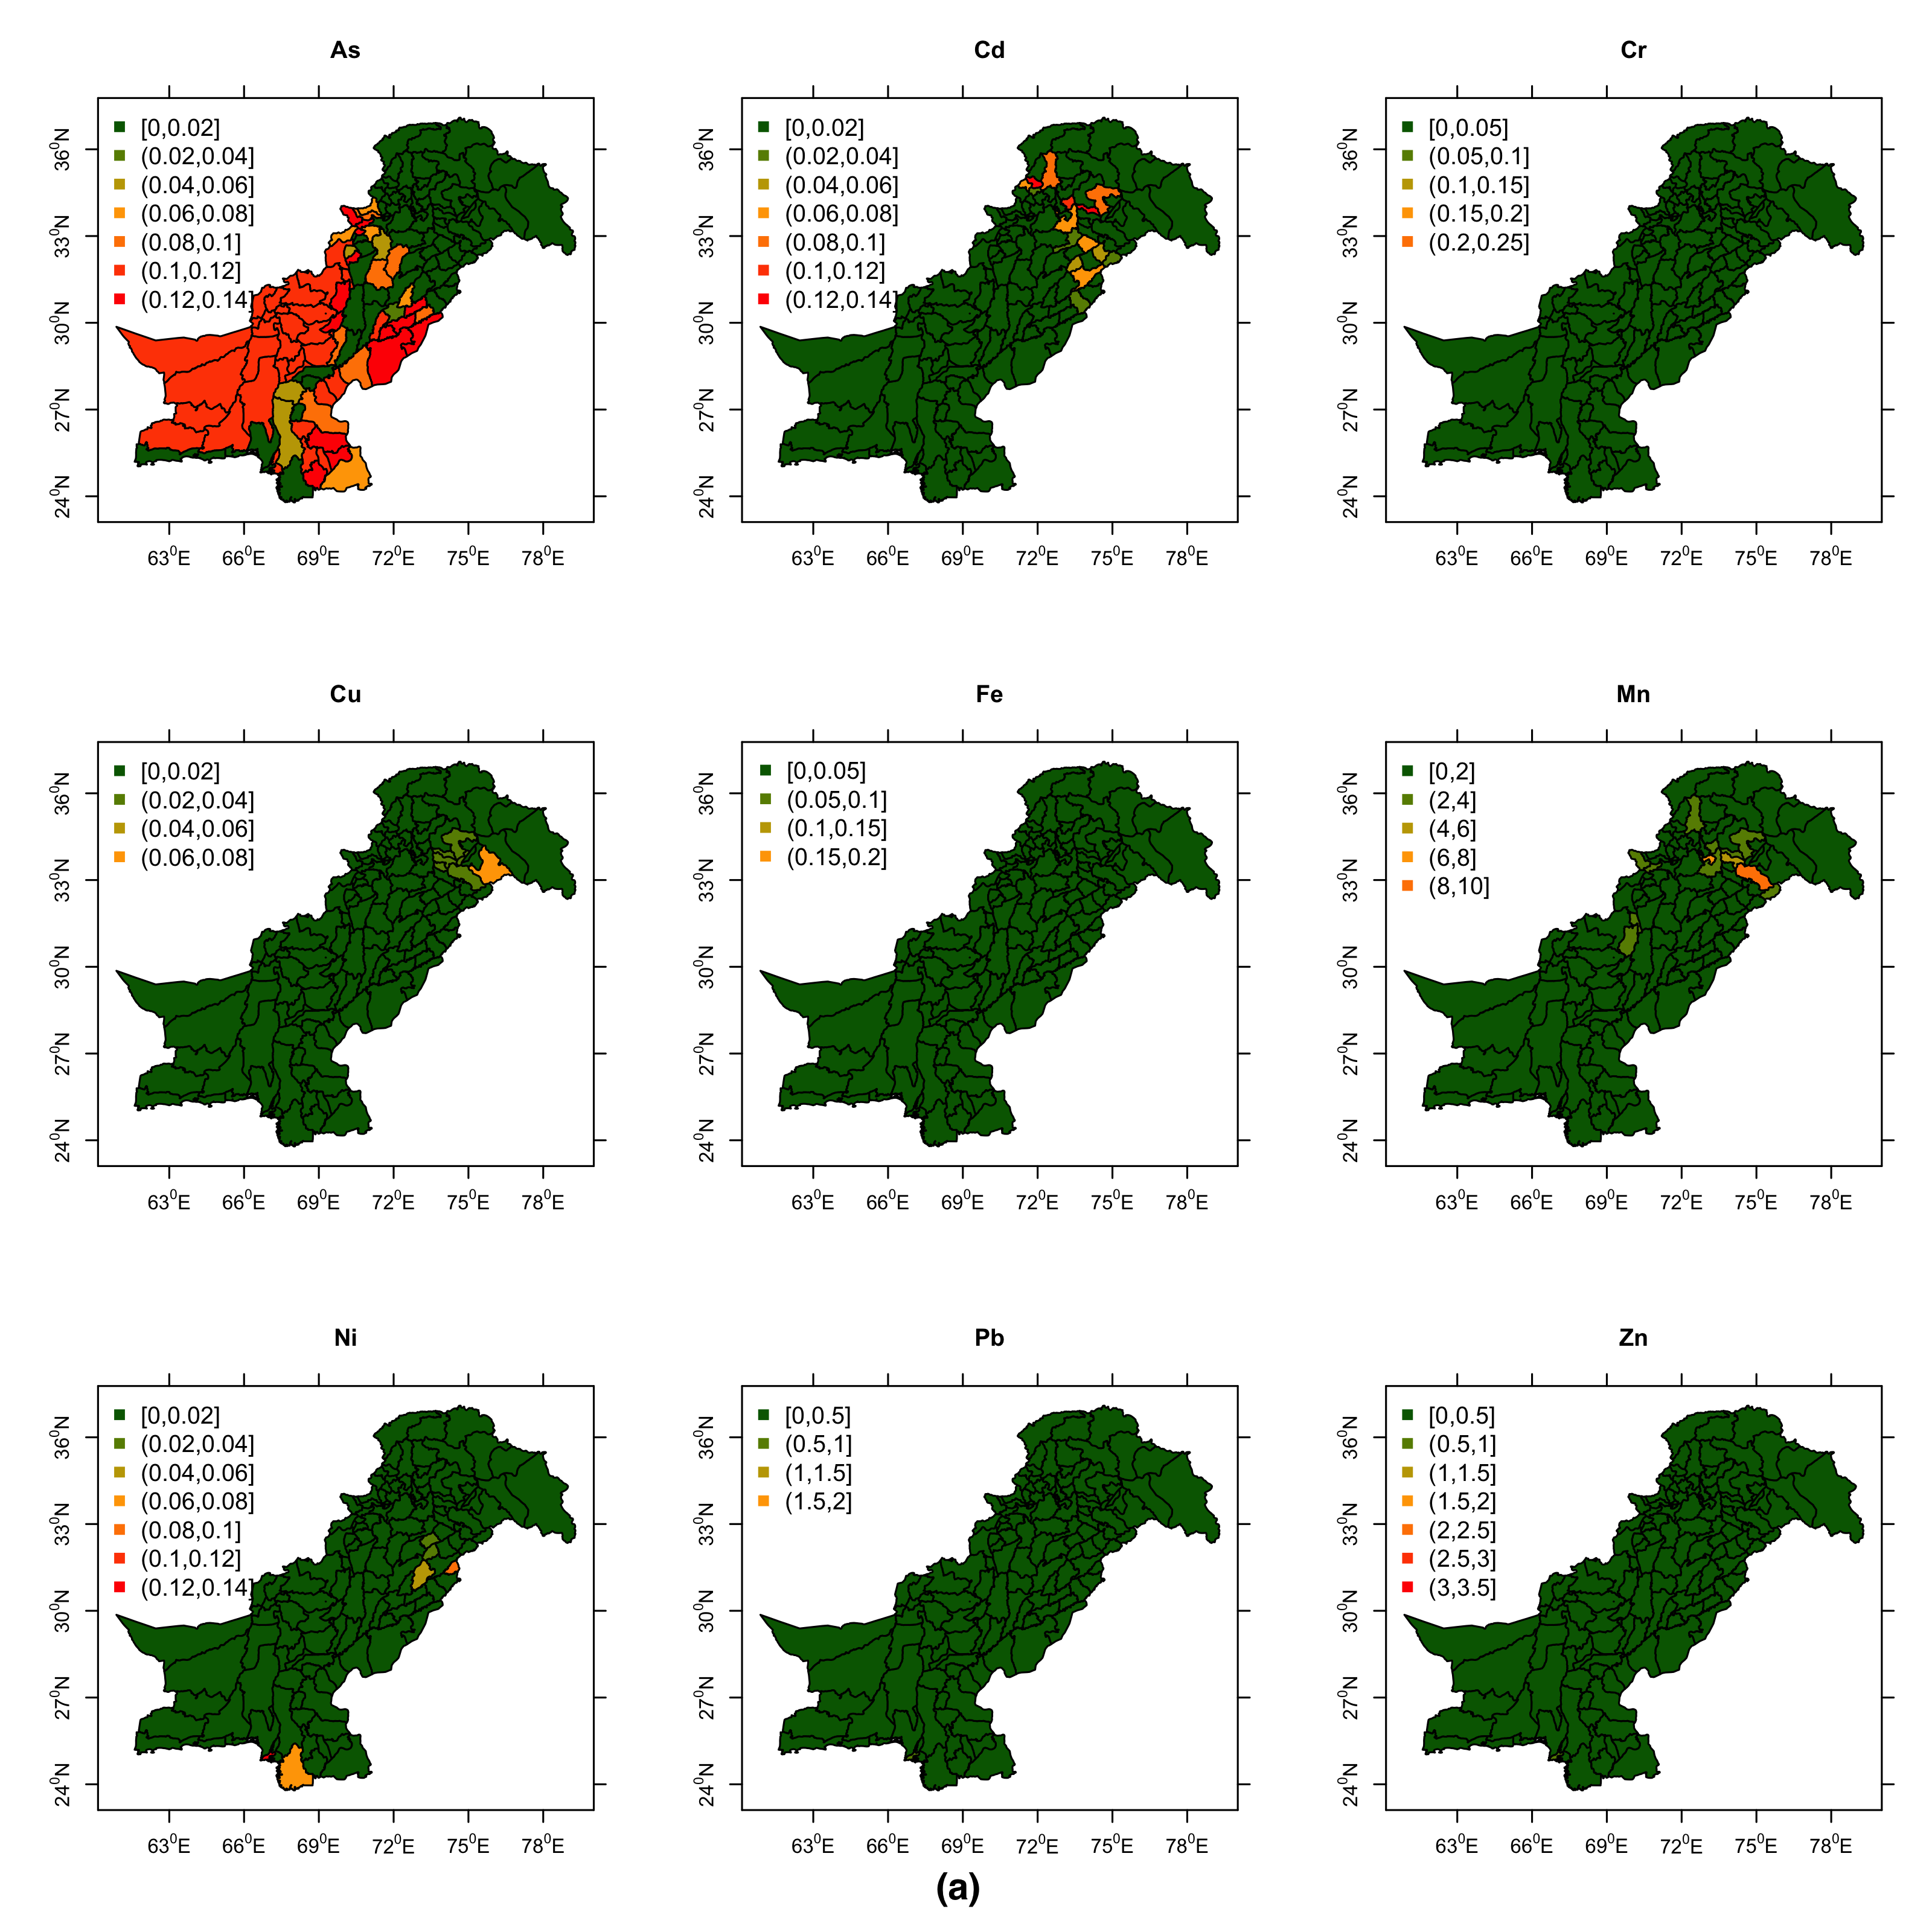
\includegraphics[width=1.1\textwidth]{Figures/Fig_D_3_a.png}
  \label{Fig_D_3_a}
\end{figure*}

\newpage

\begin{landscape}

\begin{figure}[hp!]
  \centering
  \vspace{-2.5cm} 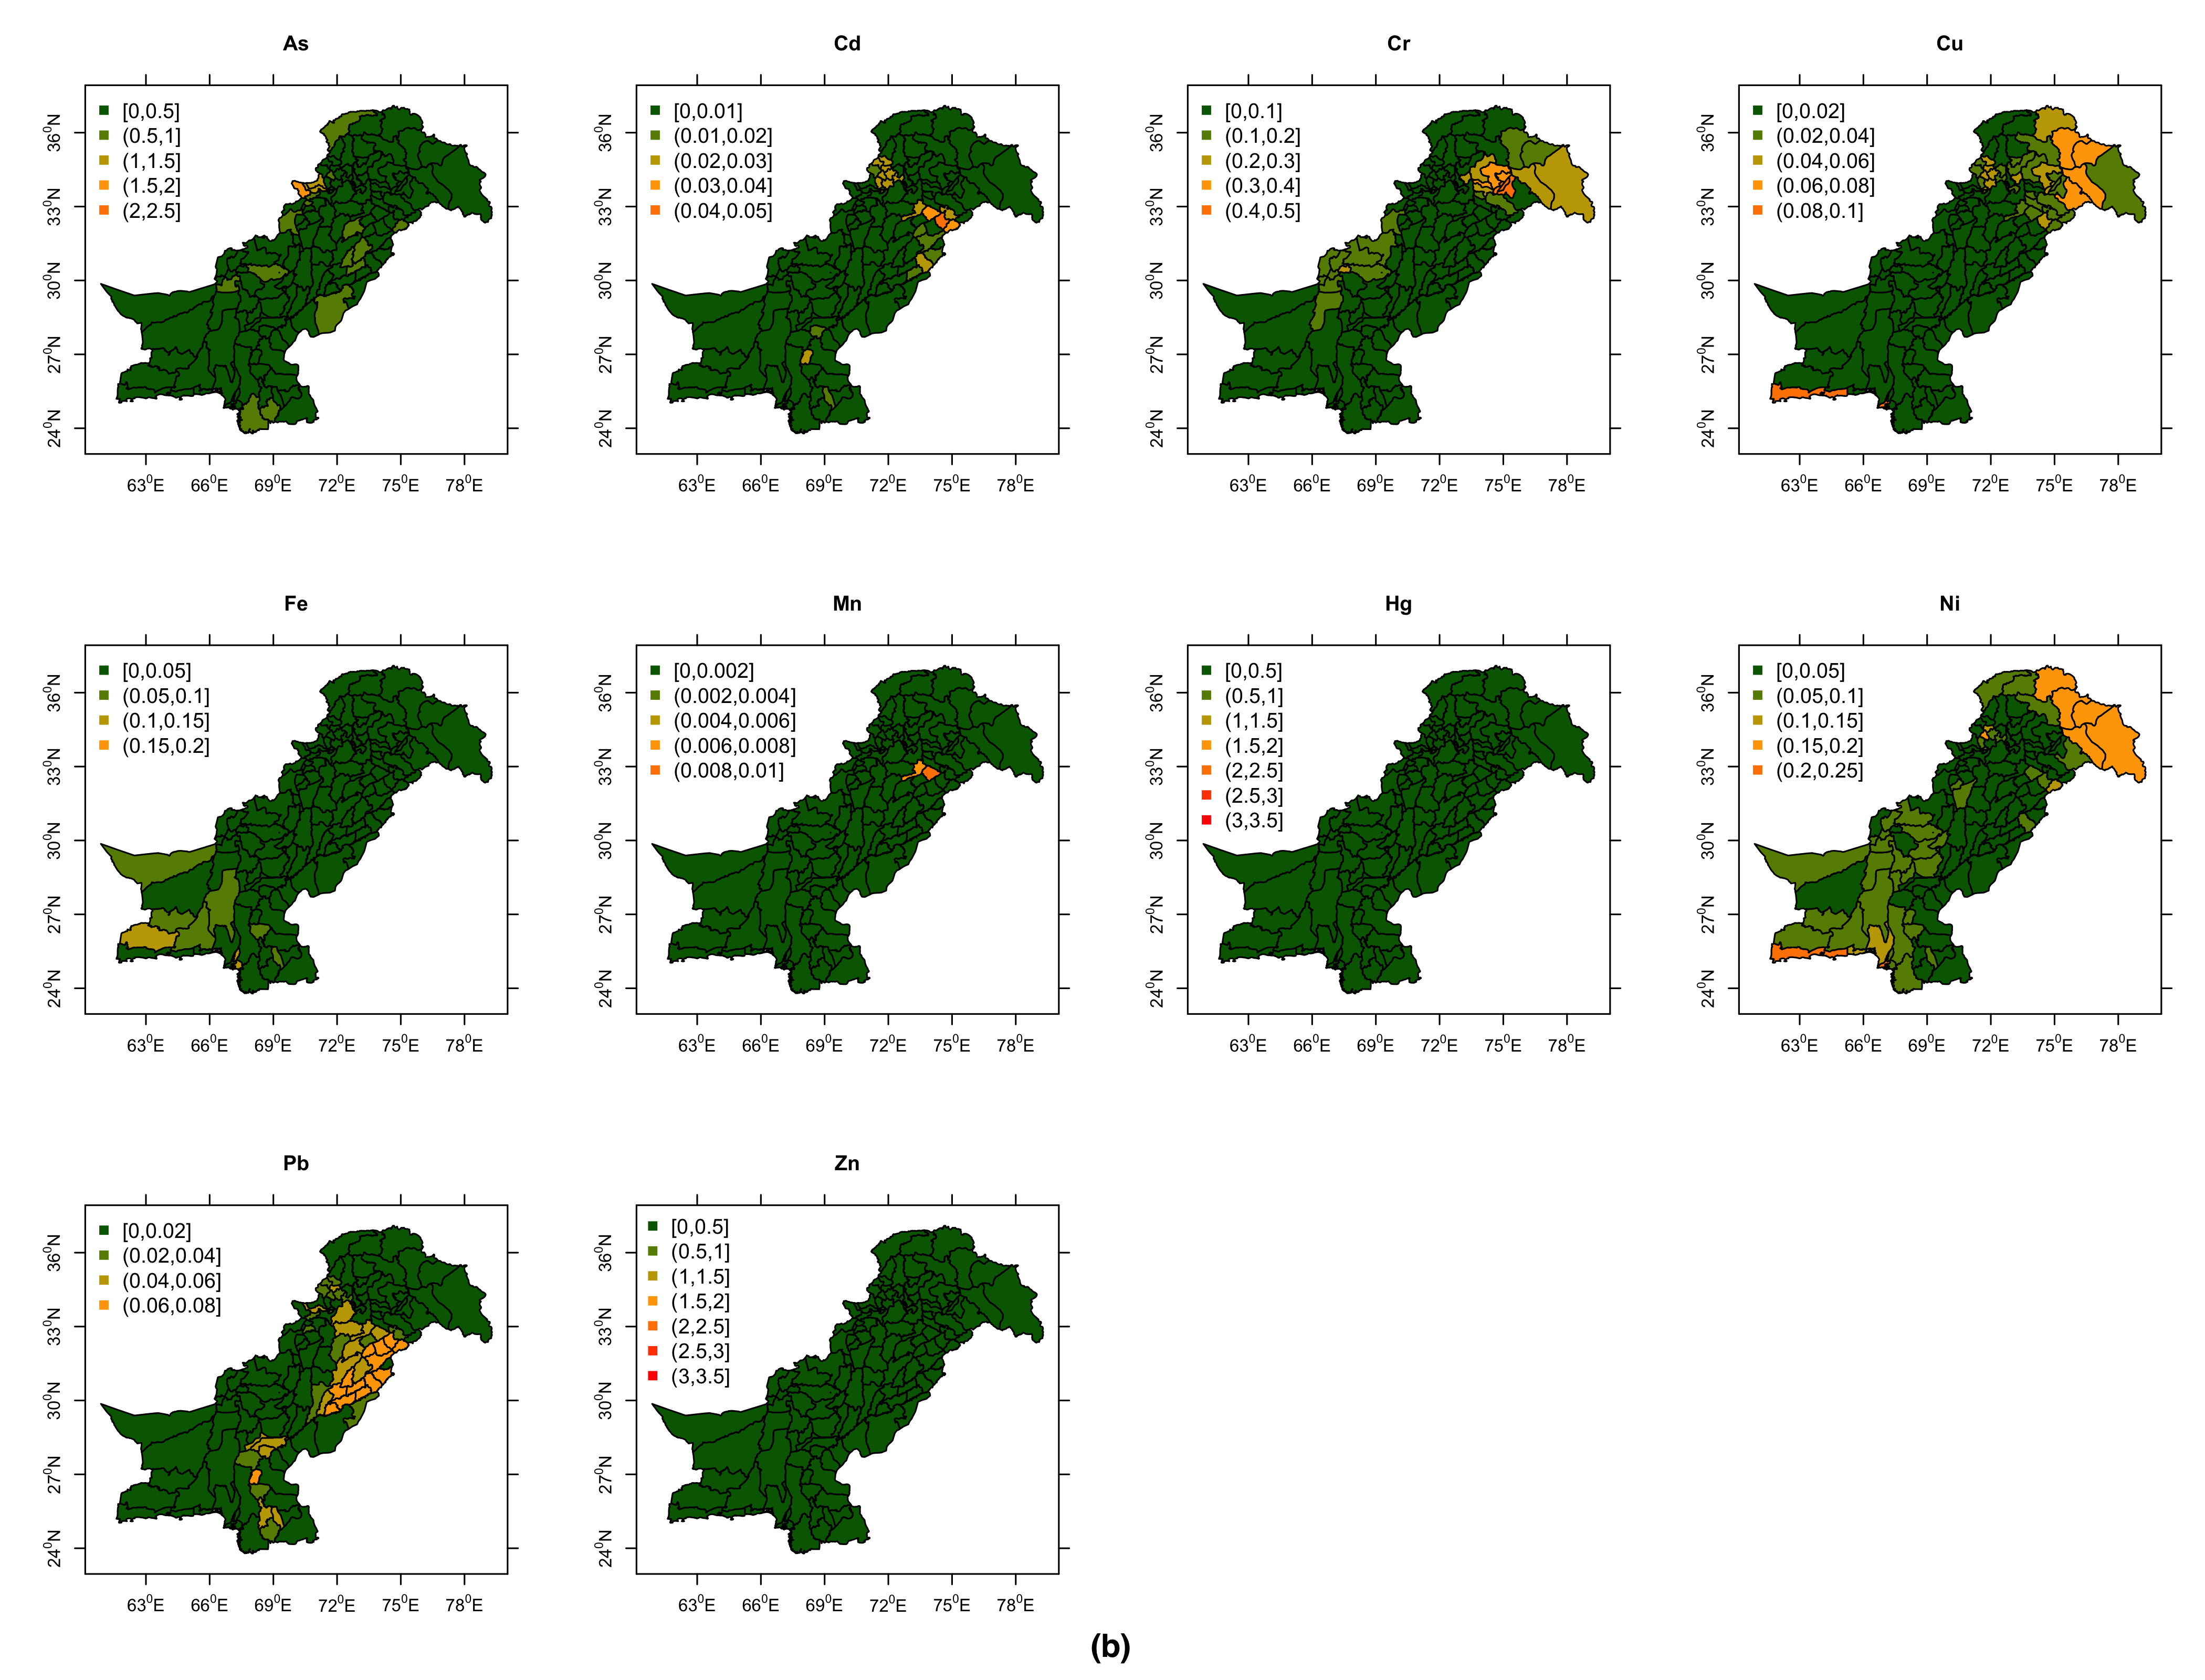
\includegraphics[width=\linewidth]{Figures/Fig_D_3_b.png}
  \caption{Lower confidence boundaries of GWR model predicted trace metal concentrations (in mg / l) within 95 \% confidence interval, i.e. predicted concentrations – 1.96 * standard errors, in (a) ground and (b) surface water at the districts of Pakistan.  The abbreviations used: As = Arsenic, Cd = Cadmium, Cr = Chromium, Cu = Copper, Fe = Iron, Mn = Manganese, Hg = Mercury, Nickel = Ni, Pb = Lead, Zn = Zinc.}
  \label{Fig_D_3_b}
\end{figure}

\end{landscape}

\newpage

\begin{figure*}[hp!]
  \centering
  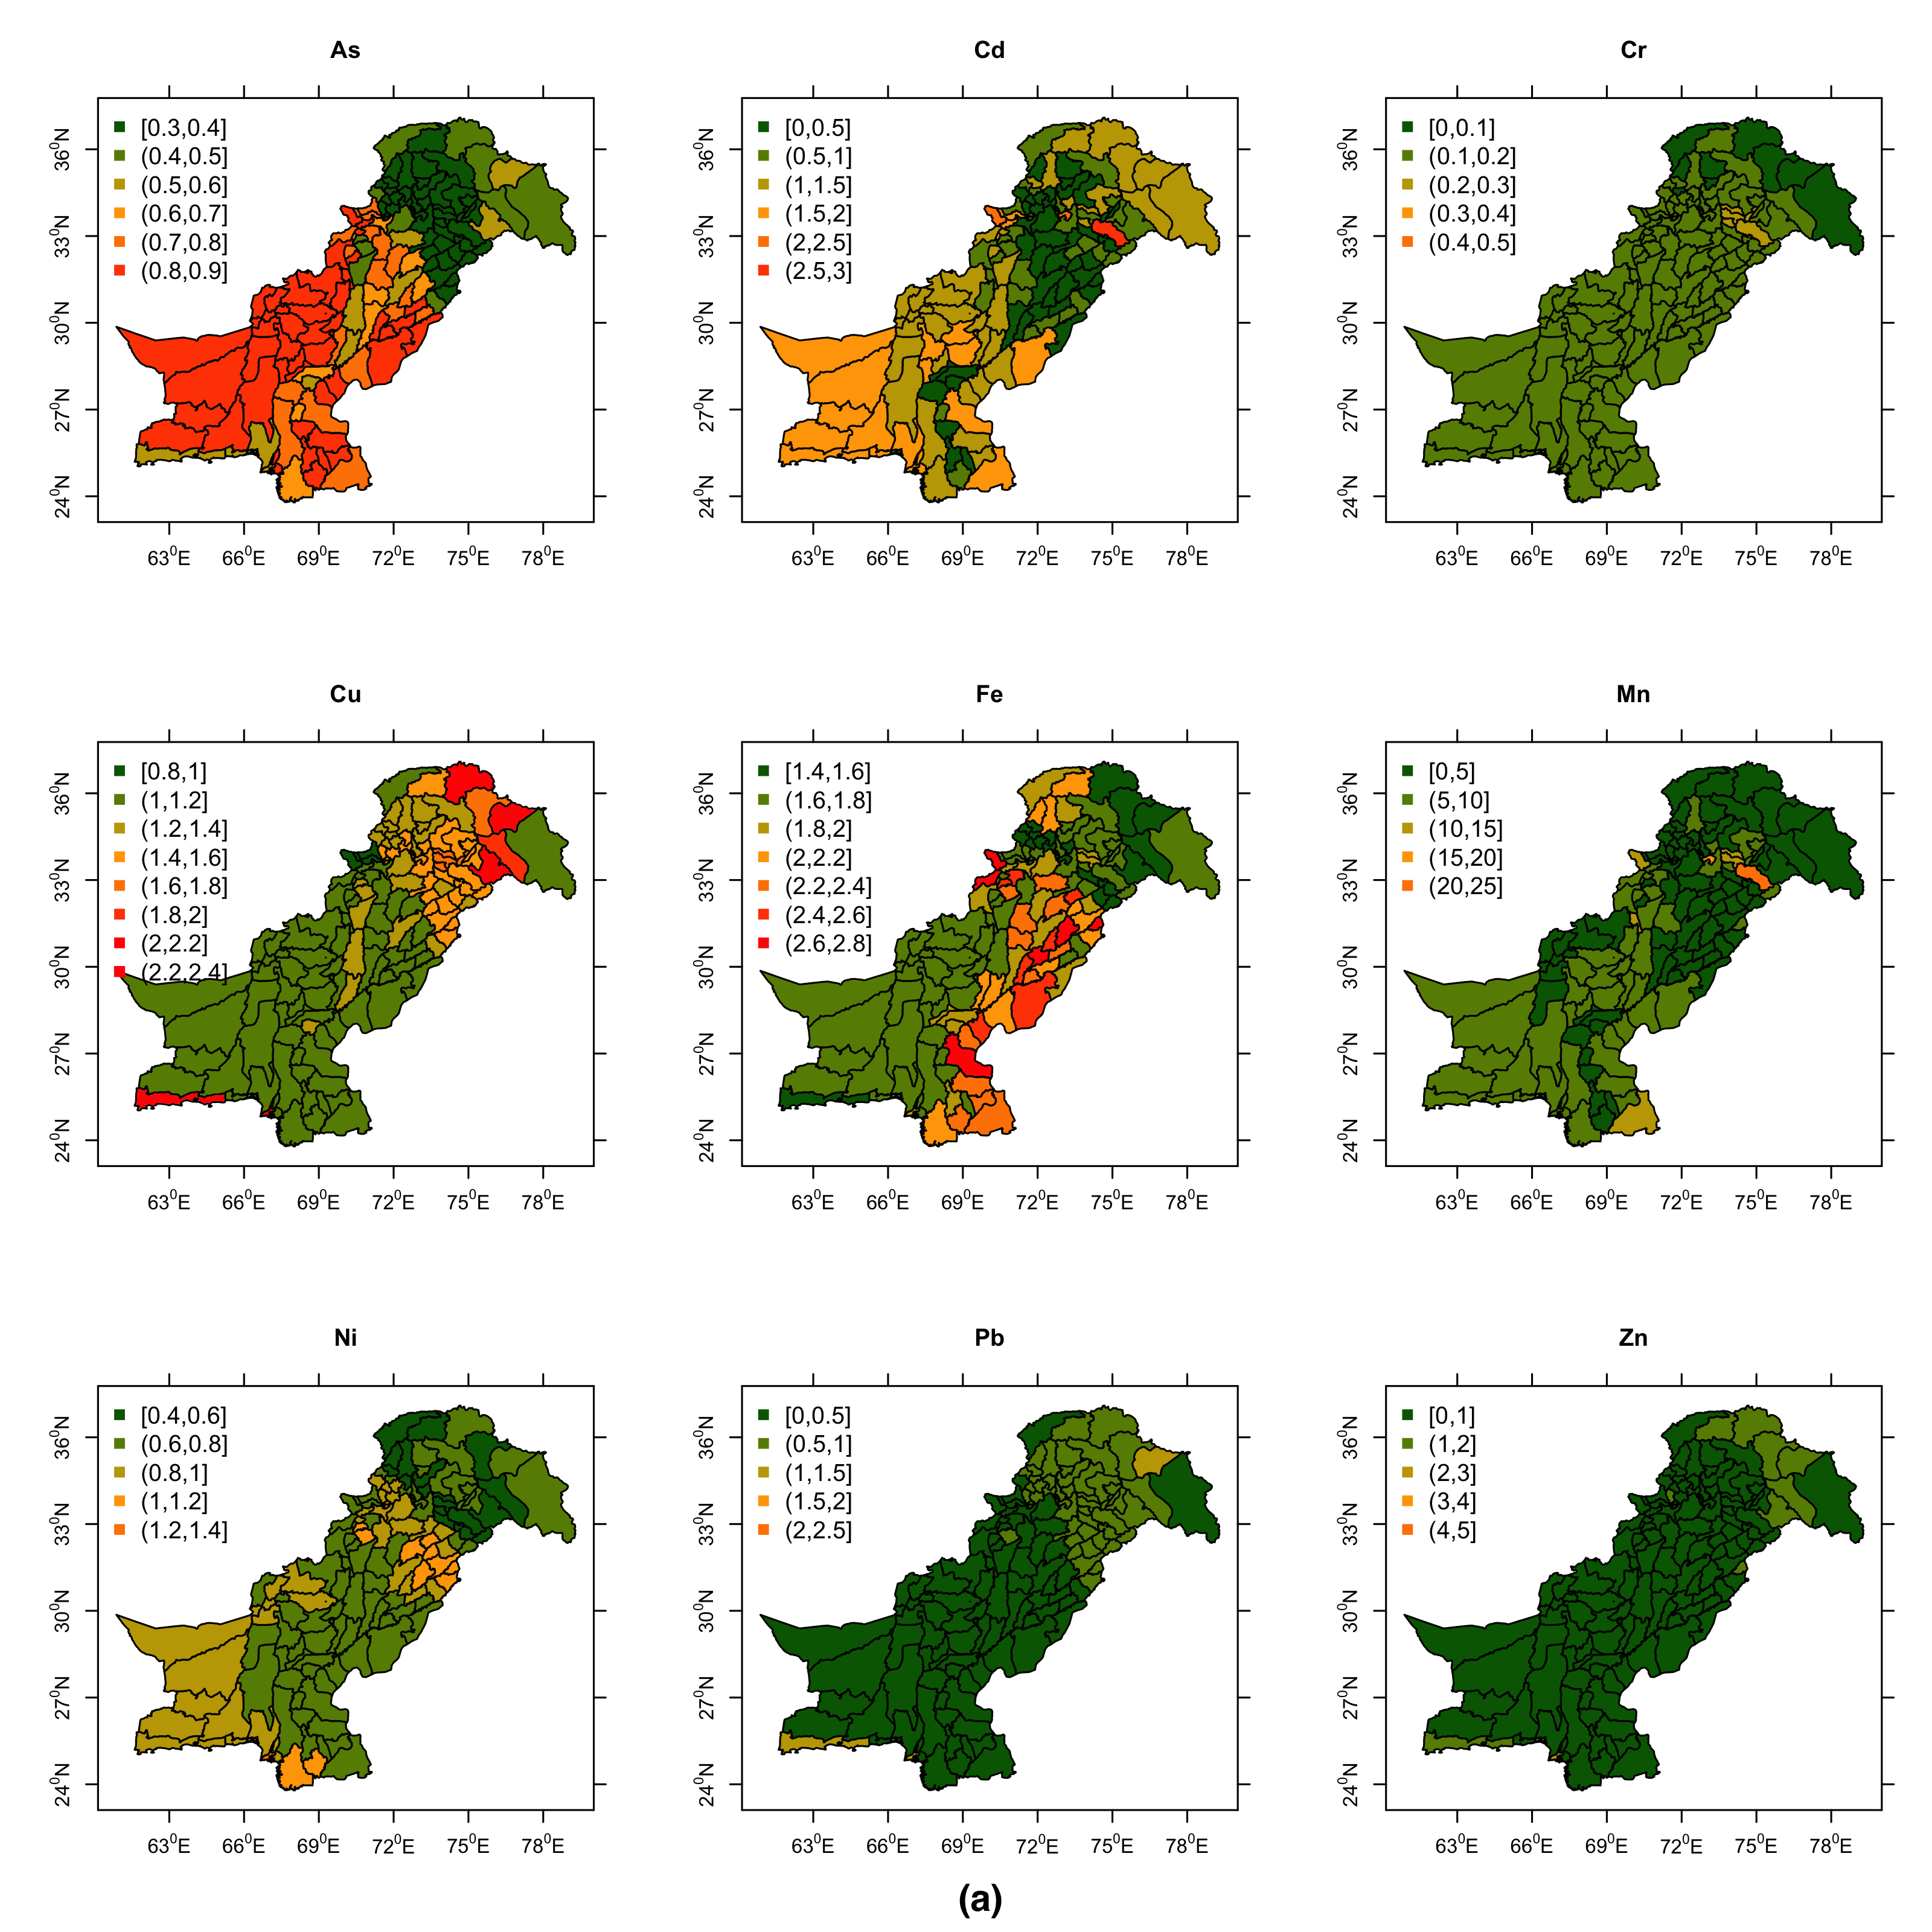
\includegraphics[width=1.1\textwidth]{Figures/Fig_D_4_a.png}
  \label{Fig_D_4_a}
\end{figure*}

\newpage

\begin{landscape}

\begin{figure}[hp!]
  \centering
  \vspace{-2.5cm} 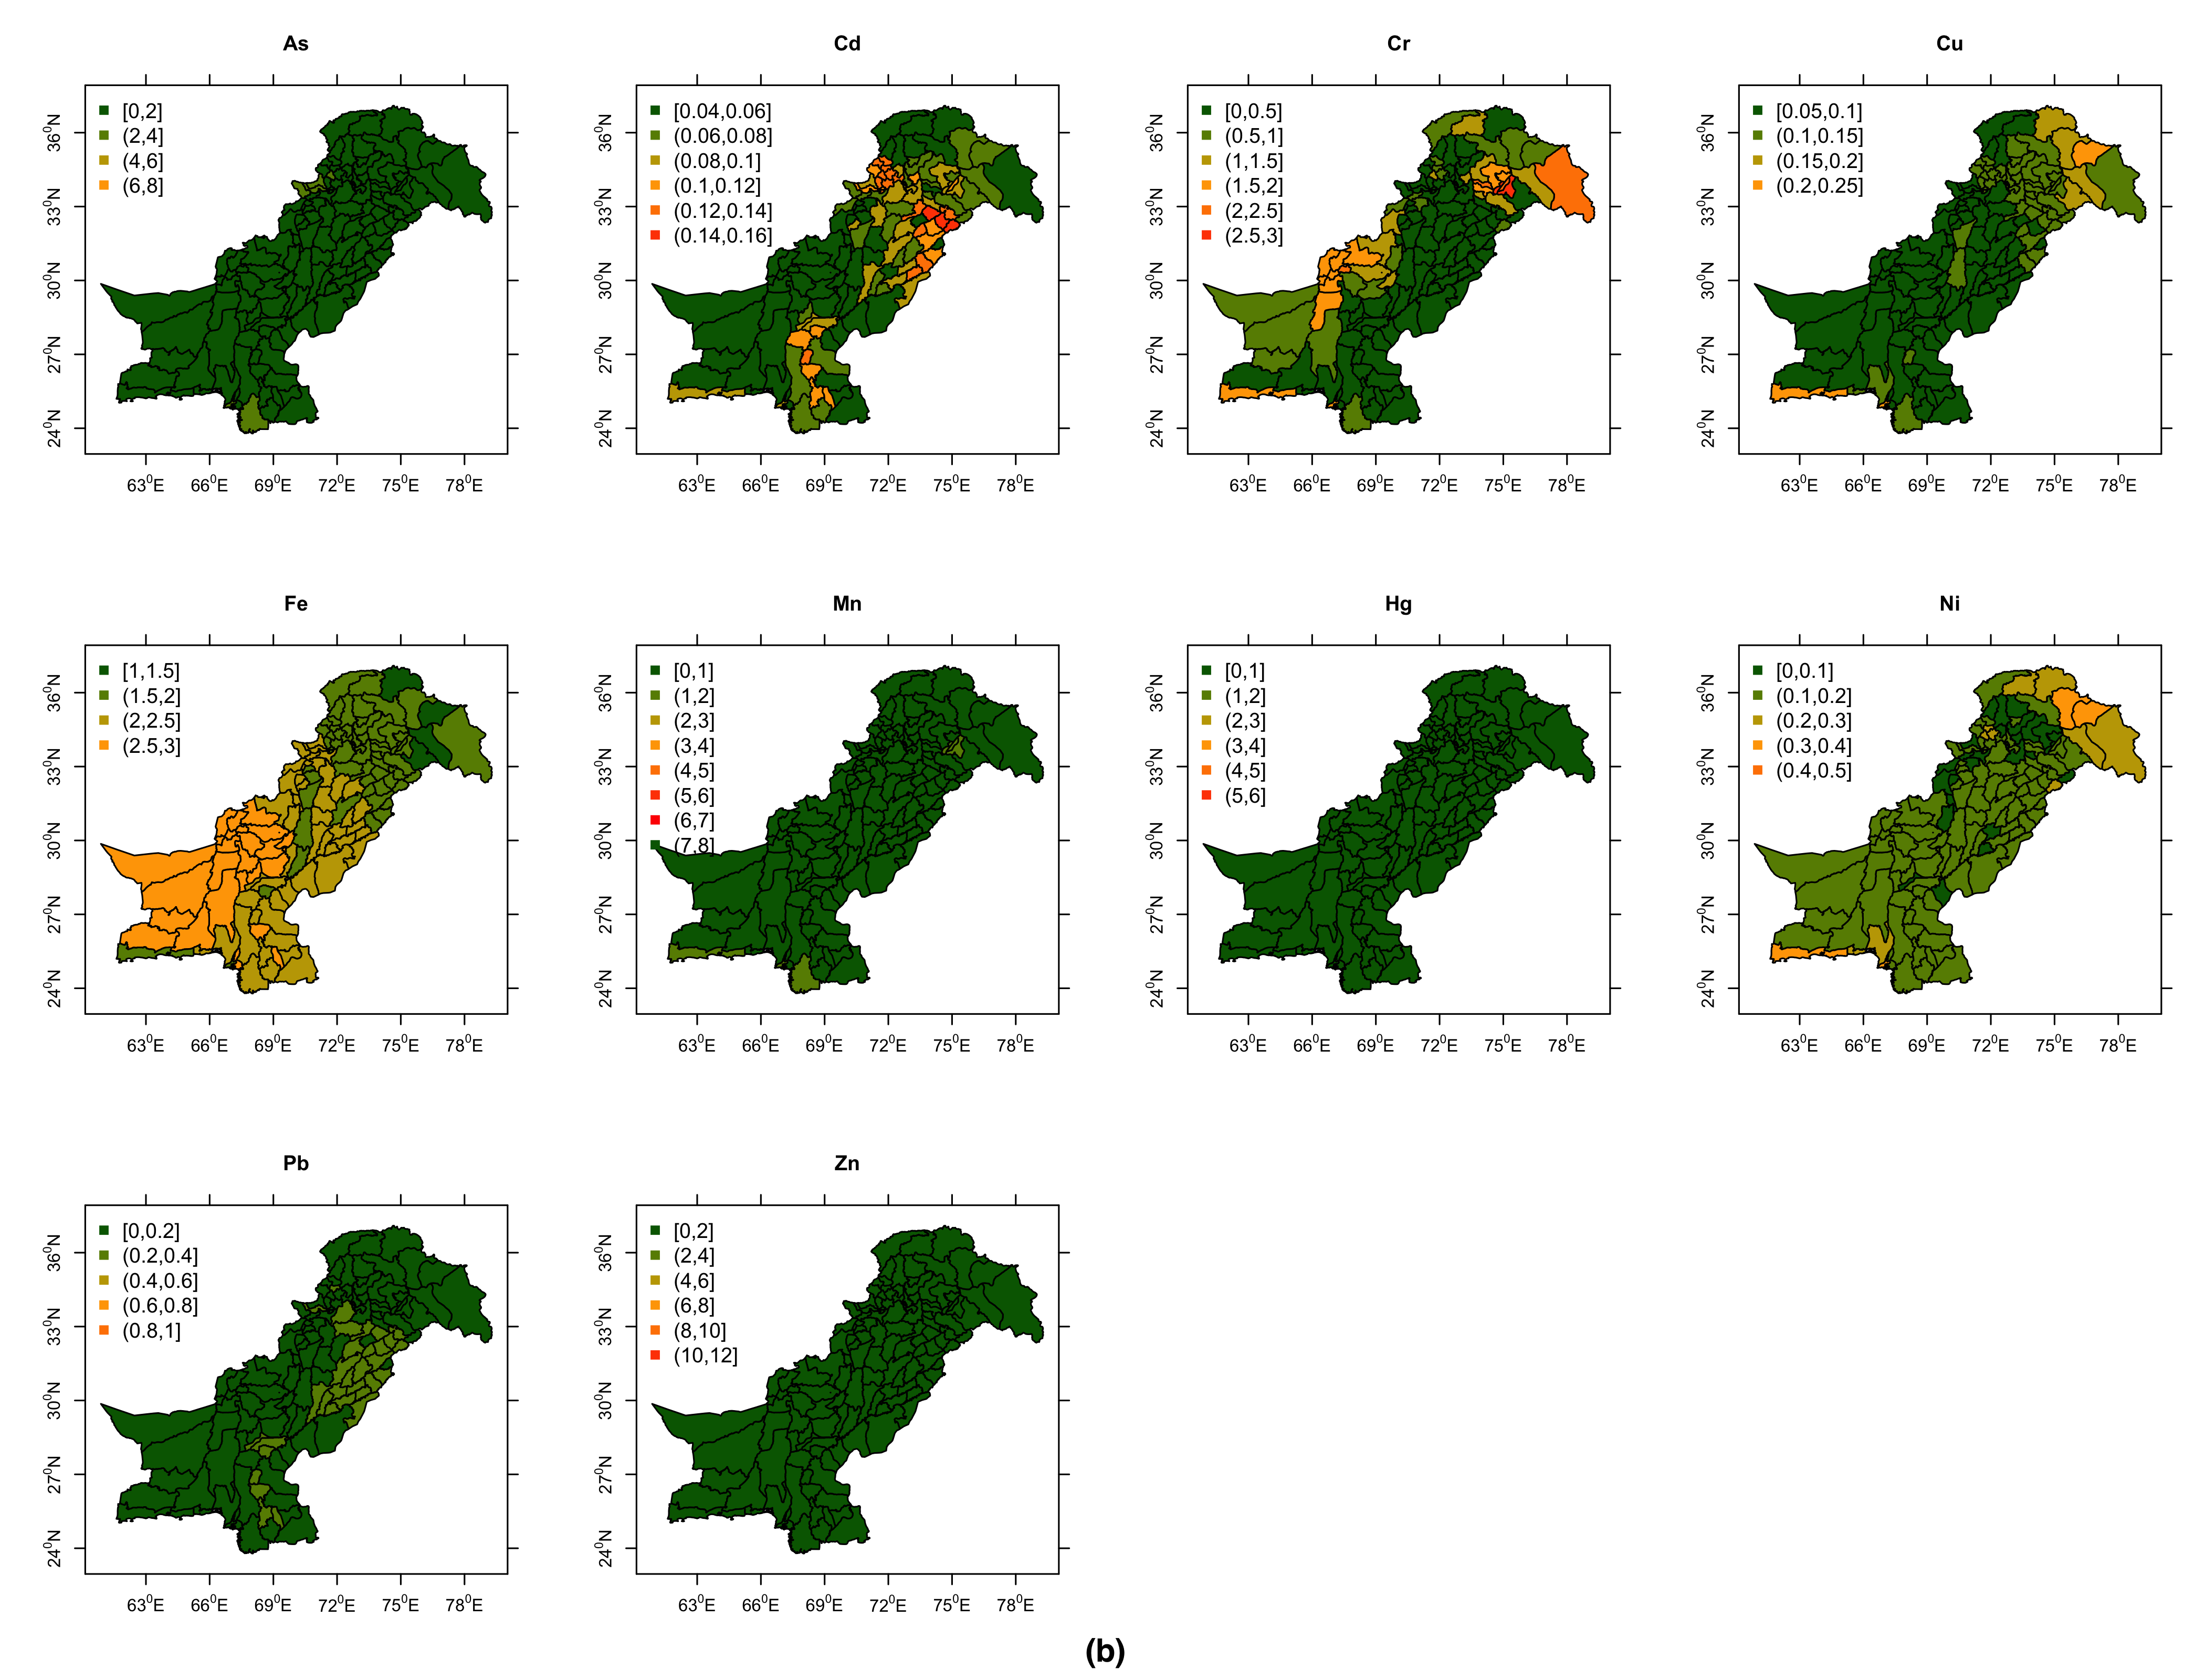
\includegraphics[width=\linewidth]{Figures/Fig_D_4_b.png}
  \caption{Upper confidence boundaries of GWR model predicted trace metal concentrations (in mg / l) within 95 \% confidence interval, i.e. predicted concentrations + 1.96 * standard errors, in (a) ground and (b) surface water at the districts of Pakistan. The abbreviations used: As = Arsenic, Cd = Cadmium, Cr = Chromium, Cu = Copper, Fe = Iron, Mn = Manganese, Hg = Mercury, Nickel = Ni, Pb = Lead, Zn = Zinc.}
  \label{Fig_D_4_b}
\end{figure}

\end{landscape}

\newpage

\begin{figure*}[hp!]
  \centering
  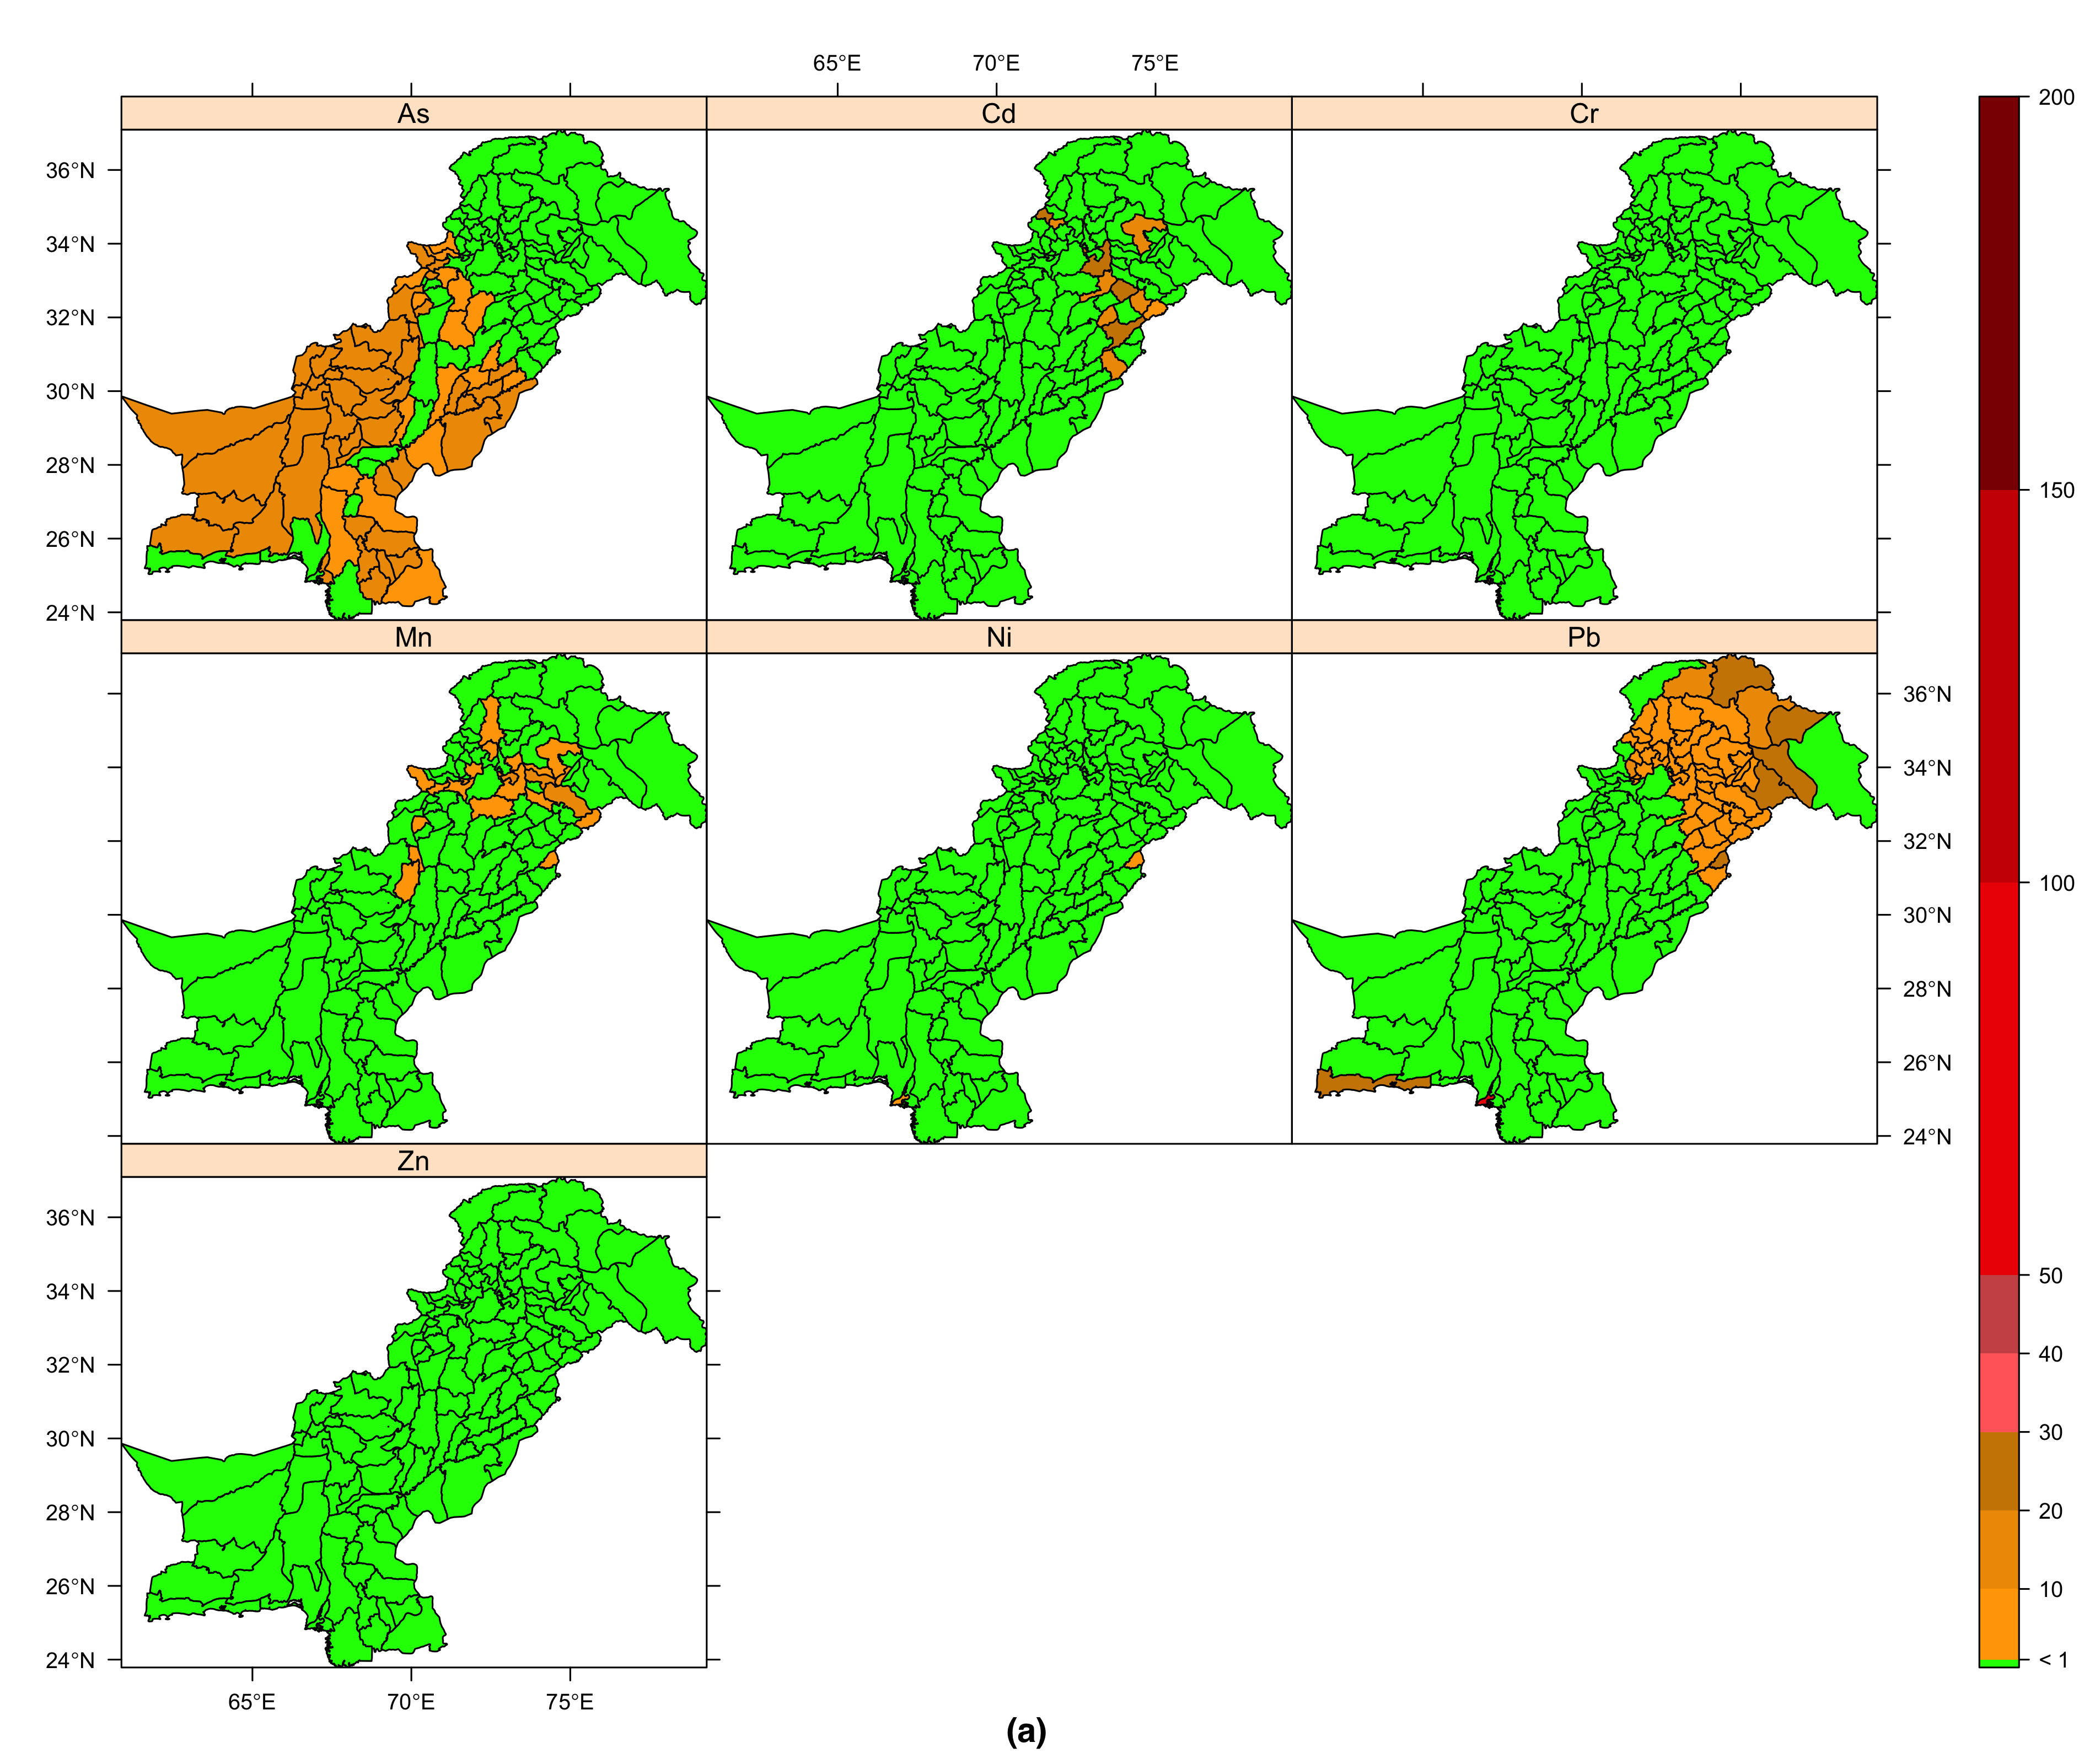
\includegraphics[width=1.1\textwidth]{Figures/Fig_D_5_a.png}
  \label{Fig_D_5_a}
\end{figure*}

\newpage

\begin{figure}[hp!]
  \centering
  \captionsetup{width=1.1\textwidth}
  \hspace{-2cm} 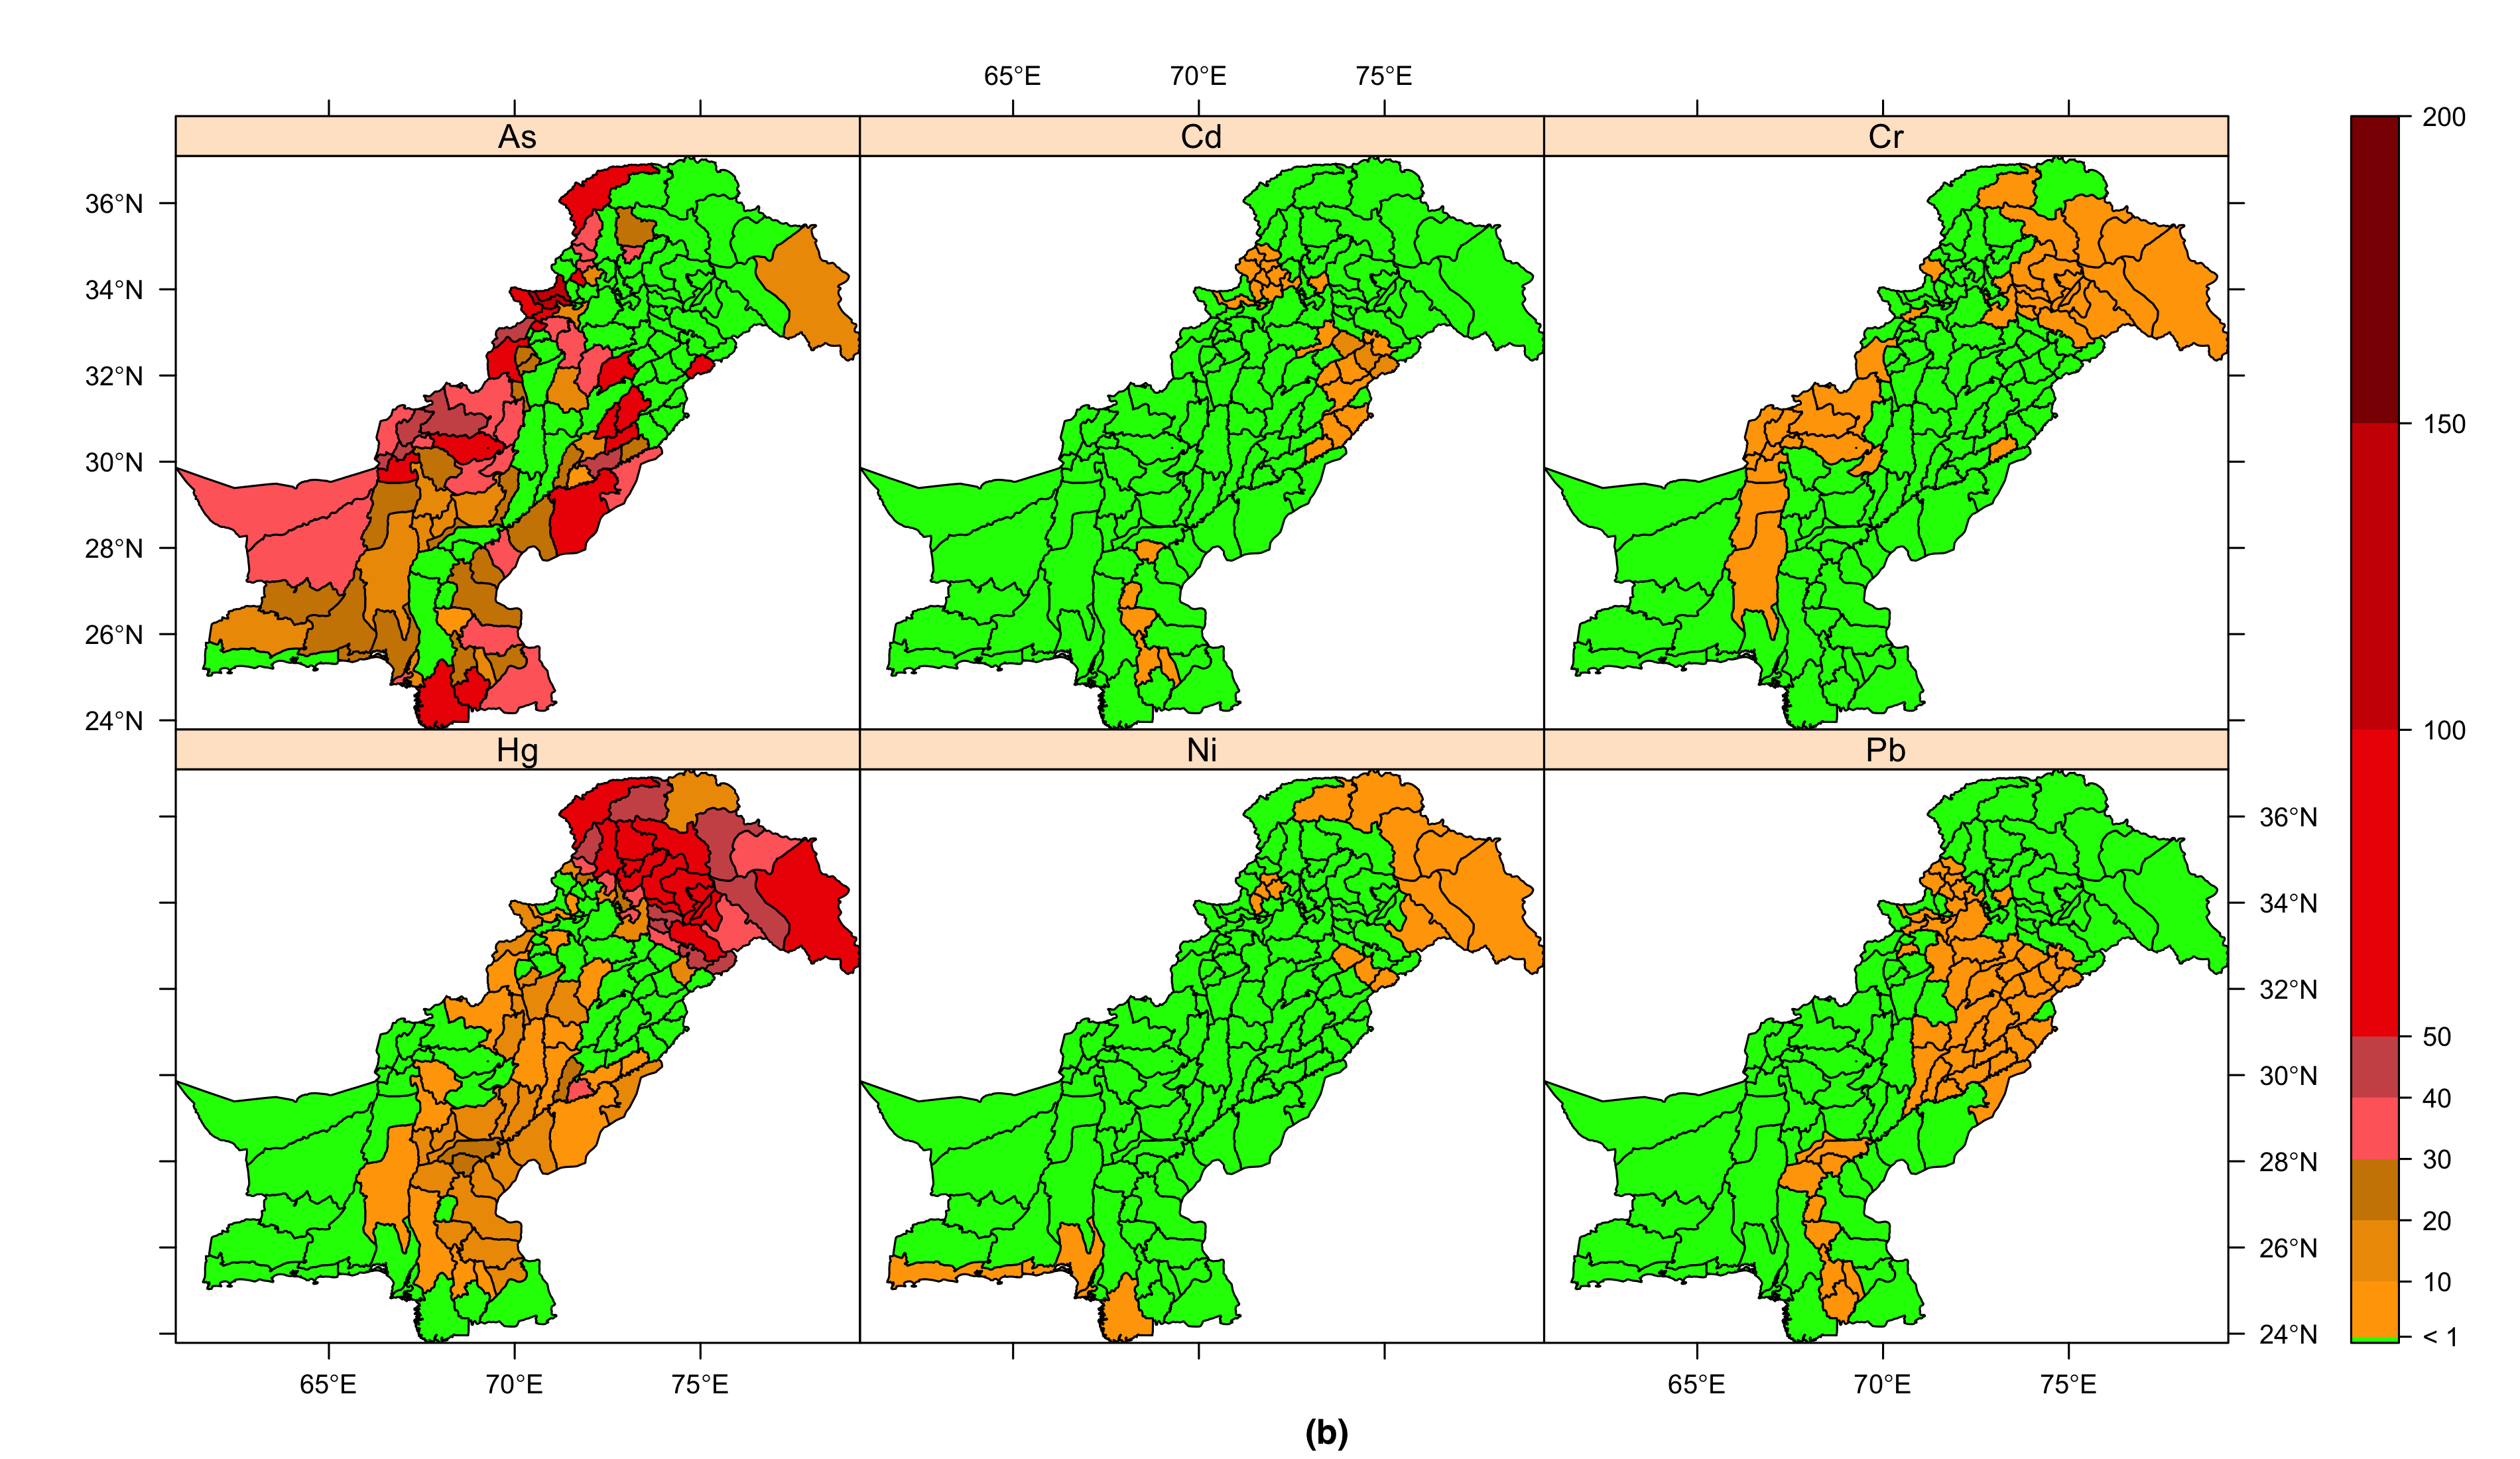
\includegraphics[width=1.1\textwidth]{Figures/Fig_D_5_b.png}
  \caption{Predicted risks, i.e. exceedances of threshold concentrations in risk quotients (RQ), for the lower confidence boundaries of GWR model predicted trace metal concentrations within 95 \% confidence interval, i.e. predicted concentrations – 1.96 * standard errors, in (a) ground and (b) surface water at the districts of Pakistan. Green indicates no exceedance, i.e. RQ $\leq$ 1. The abbreviations used: As = Arsenic, Cd = Cadmium, Cr = Chromium, Cu = Copper, Fe = Iron, Mn = Manganese, Hg = Mercury, Nickel = Ni, Pb = Lead, Zn = Zinc. Maps of Cu and Fe for ground water, and Cu, Fe, Mn and Zn for surface water are omitted because no risky district was found, i.e. for none of the districts RQ $>$ 1.}
  \label{Fig_D_5_b}
\end{figure}

\newpage

\begin{figure*}[hp!]
  \centering
  \includegraphics[width=1.1\textwidth]{Figures/Fig_D_6_a.png}
  \label{Fig_D_6_a}
\end{figure*}

\newpage

\begin{figure}[hp!]
  \centering
  \captionsetup{width=1.1\textwidth}
  \hspace{-2.0cm} \includegraphics[width=1.1\textwidth]{Figures/Fig_D_6_b.png}
  \caption{Predicted risks, i.e. exceedances of threshold concentrations in risk quotients (RQ), for the upper confidence boundaries of GWR model predicted trace metal concentrations within 95 \% confidence interval, i.e. predicted concentrations + 1.96 * standard errors, in (a) ground and (b) surface water at the districts of Pakistan. Green indicates no exceedance, i.e. RQ $\leq$ 1. The abbreviations used: As = Arsenic, Cd = Cadmium, Cr = Chromium, Cu = Copper, Fe = Iron, Mn = Manganese, Hg = Mercury, Nickel = Ni, Pb = Lead, Zn = Zinc. Map of Cu for surface water is omitted because no risky district was found, i.e. for none of the districts RQ $>$ 1.}
  \label{Fig_D_6_b}
\end{figure}

\section{Supplementary tables}
\label{Supplementary tables}

\newpage

\begin{landscape}

\begin{table}[hp!]

\label{Table D.1}

\caption{Observed concentration values (mg / l) of the trace metals in ground water samples from different districts of Pakistan during 1997-2014. The years of observed concentrations refer to the publication years of corresponding studies.}

\centering

\begin{threeparttable}

\begin{tabular}{>{\centering\arraybackslash}m{3.3cm}>{\centering\arraybackslash}m{0.5cm}>{\centering\arraybackslash}m{0.9cm}>{\centering\arraybackslash}m{0.8cm}>{\centering\arraybackslash}m{0.9cm}>{\centering\arraybackslash}m{0.8cm}>{\centering\arraybackslash}m{0.9cm}>{\centering\arraybackslash}m{1.0cm}>{\centering\arraybackslash}m{0.9cm}>{\centering\arraybackslash}m{0.9cm}>{\centering\arraybackslash}m{0.9cm}>{\centering\arraybackslash}m{0.9cm}>{\centering\arraybackslash}m{4.4cm}}

\toprule
\textbf{Sampling location} & \textbf{n} & \multicolumn{10}{c}{\textbf{Mean concentration}} & \textbf{Study}\\
\textbf{(district)} & & \multicolumn{10}{c}{\textbf{(mg/l)}} & \\
 & & \textbf{As} & \textbf{Hg} & \textbf{Ni} & \textbf{Cu} & \textbf{Mn} & \textbf{Cr} & \textbf{Fe} & \textbf{Zn} & \textbf{Cd} & \textbf{Pb} & \\

\midrule

Lahore & 30 & 0.121 & - & - & - & - & - & - & - & - & - & Sultana et al., 2013\\
Kasur & 65 & < DL & - & 0.13 & 1.3 & 1.06 & 0.01 & 3.7 & 1.84 & < DL & 0.12 & Mahmood and Maqbool, 2006\\
Kasur  & 24 & 0.113 & - & - & - & - & - & - & - & - & - & Farooqi et al., 2007 b\\
Dera Ghazi Khan & 32 & 0.029 & - & - & - & - & - & - & - & - & - & Malana et al., 2011\\
Muzaffargarh  & 49 & 0.071 & - & - & - & - & - & - & - & - & - & Nickson et al., 2005\\
Multan & 3 & 0.53 & - & < DL & < DL & 0.53 & < DL & 1.4 & < DL & < DL & < DL & Nickson et al., 2005\\
Faislabad & 26 & < DL & - & 0.96 & 0.21 & 1.22 & 0.14 & 0.16 & 0.13 & 0.04 & 0.33 & Midrar-ul-Haq et al., 2005\\
Kalanlawala & 24 & 0.966 & - & < DL & < DL & < DL & < DL & < DL & < DL & - & < DL & Farooqi et al., 2007a\\
Sialkot & 25 & < DL & - & 0.1 & 0.06 & 0.03 & 0.03 & 0.18 & 0.16 & - & 0.49 & Ullah et al., 2009\\
Jamshoro & 45 & 0.08 & - & - & - & - & - & 0.79 & < DL & - & < DL & Baig et al., 2009\\
Therparkar & 140 & 0.75 & - & - & - & - & - & - & - & - & - & Brahman et al.,  2013\\
South East Sindh & 25 & 0.0633 & - & - & - & - & - & - & - & - & - & Kazi et al., 2009\\
Karachi & - & 0.08 & 0.01 & 0.5 & 0.09 & < DL & 0.34 & < DL & 4.02 & 0.04 & 2 & Rehman et al.,1997\\
Nowshera & 44 & < DL & 0.001 & 1.43 & 0.67 & 1.56 & 0.155 & 0.22 & 0.22 & 0.155 & 0.375 & Midrar-ul-Haq et al., 2005\\
Charsadda & 951 & < DL & < DL & 0.0094 & 0.071 & < DL & 0.0188 & 0.372 & 0.36 & 0.0053 & 0.0638 & Khan et al., 2012\\
Charsadda & 315 & - & - & 0.0007 & 0.289 & - & 0.0139 & 0.0549 & 0.135 & 0.0007 & 0.0089 & Khan et al., 2013\\
Swabi & 3 & - & - & 0.048 & 0.893 & 0.16 & 0.128 & 0.0205 & 0.0205 & 0.016 & 0.705 & Nasrullah et al., 2006\\
Peshawar & 4 & - & - & 0.88 & 0.36 & 0.12 & 0.089 & 0.143 & 0.131 & 0.03 & 0.66 & Tariq et al., 2006\\
Kohistan & 37 & 0.0021 & - & - & - & - & - & 0.327 & - & - & - & Muhammad et al., 2010\\
Kohistan & 10 & - & - & 0.0001 & 0.077 & 0.0013 & 2E-05 & - & 0.262 & 0.0001 & 0.0007 & Muhammad et al., 2011\\
Mohamnd Agency & 51 & - & - & 0.04 & 2.4 & 0.3 & 0.2 & 0.05 & 0.024 & 0.0006 & 0.0009 & Shah et al., 2012\\
Shiekhupura & - & 0.39 & - & - & 0.21 & 0.28 & - & - & - & 0.36 & - & Qazi et al., 2014\\

\bottomrule

WHO drinking water effect-threshold & & 0.01 & 0.001 & 0.02 & 2 & 0.5 & 0.05 & 0.3 & 3 & 0.003 & 0.01 & WHO, 2011\\
\hline

\end{tabular}
\begin{tablenotes}
\footnotesize
n= number of sites, As = Arsenic, Cd = Cadmium, Cr = Chromium, Cu = Copper, Fe = Iron, Mn = Manganese, Hg = Mercury, Nickel = Ni, Pb = Tin, Zn = Zinc, - = not sampled or not known, DL = detection limit, WHO=World Health Organization.
\end{tablenotes}
\end{threeparttable}
\end{table}

\clearpage

\begin{table}[hp!]

\label{Table D.2}

\vspace{-1.3cm} 

\caption{Observed concentration values (mg / l) of the trace metals in surface water samples from different districts of Pakistan during 1991-2014. The years of observed concentrations refer to the publication years of corresponding studies.}

\centering

\begin{threeparttable}

\begin{tabular}{>{\centering\arraybackslash}m{3.3cm}>{\centering\arraybackslash}m{0.5cm}>{\centering\arraybackslash}m{0.9cm}>{\centering\arraybackslash}m{0.8cm}>{\centering\arraybackslash}m{0.9cm}>{\centering\arraybackslash}m{0.8cm}>{\centering\arraybackslash}m{0.9cm}>{\centering\arraybackslash}m{1.0cm}>{\centering\arraybackslash}m{0.9cm}>{\centering\arraybackslash}m{0.9cm}>{\centering\arraybackslash}m{0.9cm}>{\centering\arraybackslash}m{0.9cm}>{\centering\arraybackslash}m{4.2cm}}

\toprule
\textbf{Sampling location} & \textbf{n} & \multicolumn{10}{c}{\textbf{Mean concentration}} & \textbf{Study}\\
\textbf{(district)} & & \multicolumn{10}{c}{\textbf{(mg/l)}} & \\
 & & \textbf{As} & \textbf{Hg} & \textbf{Ni} & \textbf{Cu} & \textbf{Mn} & \textbf{Cr} & \textbf{Fe} & \textbf{Zn} & \textbf{Cd} & \textbf{Pb} & \\

\midrule

Islamabad & 50 & - & - & - & 0.017 & 0.013 & 0.097 & 0.076 & 0.0132 & 0.0075 & 0.0446 & Iqbal et al., 2014\\
Mohmand Agency & 51 & - & - & 0.1052 & 0.06 & 0.35 & 0.32 & 0.158 & 0.0128 & 0.0005 & 0.001 & Shah et al., 2012\\
Kohistan & 18 & 0.0007 & - & - & - & - & - & 0.447 & - & - & - & Muhammad et al., 2010\\
Kohistan & 8 & - & - & 0.0003 & 0.082 & 0.0005 & 0.0001 & - & 0.015 & 0.0001 & 0.0003 & Muhammad et al., 2011\\
Islamabad  & 30 & - & - & 0.51 & 0.08 & 0.26 & 1.17 & 30.04 & 3.45 & 0.06 & 0.41 & Malik et al., 2010\\
Mianwali & - & 0.75 & 0.017 & 0.065 & 0.004 & 0.004 & 0.071 & 0.004 & 0.029 & 0.003 & 0.058 & Ashraf et al., 1991\\
Mianwali & - & - & - & 0.127 & - & - & - & - & 0.174 & - & - & Tariq et al., 1996\\
Muzaffargarh & 30 & 0.0011 & 0.053 & 0.127 & 0.011 & 0.016 & 0.018 & 1.548 & 0.01 & 0.016 & 0.125 & Tariq et al., 1995\\
Muzaffargarh & 25 & 0.007 & < DL & - & - & 0.28 & - & 0.18 & - & - & - & Nickson et al., 2005\\
Sukhar & 12 & 0.62 & 0.14 & 0.061 & 0.004 & 0.018 & 0.002 & 0.012 & 0.028 & 0.002 & 0.107 & Ashraf et al., 1991\\
Lahore & 45 & 0.0018 & 0.0006 & 0.00125 & 0.006 & 0.0055 & 0.0009 & 0.0845 & 0.022 & 0.0008 & 0.001 & Tariq et al., 1994\\
Lahore & - & - & - & 0.93 & 0.45 & 0.85 & 0.07 & 8 & 1.7 & 0.18 & 0.03 & Kashif et al., 2009\\
Kalar Kahar  & 25 & - & - & 0.0325 & 0.006 & - & - & 2.83 & 1.63 & 0.03 & 0.155 & Raza et al., 2007\\
Sehwan & 20 & - & - & 0.0027 & 0.0084 & - & - & 0.0151 & 0.0057 & 0.0091 & 0.0068 & Mastoi et al., 2008\\
Manchar Lake & 80 & 0.102 & - & 0.0043 & 0.0089 & - & - & 0.0012 & 0.0157 & 0.001 & 0.009 & Mastoi et al., 2008\\
Manchar Lake & 160 & 0.0811 & - & 0.017 & 0.019 & 0.0732 & 0.0075 & 3 & 3 & 0.0108 & 0.0833 & Kazi et al., 2009\\
Jamshoro & 45 & 0.042 & - & - & - & - & - & 0.19 & 1.489 & - & - & Baig et al., 2009\\
Jamshoro & 58 & 0.075 & - & - & - & - & - & 2.34 & - & - & - & Arain et al., 2009(b)\\
Besham & - & - & - & 0.253 & - & - & - & - & 0.016 & - & - & Tariq et al., 1996\\
Chagai & - & - & - & 0.096 & - & - & - & - & 0.028 & - & - & Tariq et al., 1996\\
Khushalgarh & - & - & - & 0.075 & - & - & - & - & 0.018 & - & - & Tariq et al., 1996\\
Dera Gazi Khan & - & - & - & 0.124 & - & - & - & - & 0.172 & - & - & Tariq et al., 1996\\
Gilgit & 22 & 0.0025 & 0.135 & 0.245 & 0.091 & 0.013 & 0.017 & 0.041 & 0.011 & 0.002 & 0.013 & Tariq et al., 1995\\
Jacobabad & 34 & 0.0008 & 0.21 & 0.124 & 0.04 & 0.015 & 0.034 & 0.034 & 0.011 & 0.011 & 0.038 & Tariq et al., 1995\\
Sialkot & 40 & 0.0013 & 0.208 & 0.124 & 0.026 & 0.209 & 0.018 & 0.209 & 0.062 & 0.014 & 0.073 & Tariq et al., 1996\\
Sialkot & - & - & - & 0.1 & 0.2 & - & - & 0.8 & 0.1 & 0.3 & 0.2 & Qadir et al., 2008\\

\bottomrule

WHO drinking water effect-threshold & & 0.01 & 0.001 & 0.02 & 2 & 0.5 & 0.05 & 0.3 & 3 & 0.003 & 0.01 & WHO, 2011\\
\hline

\end{tabular}
\begin{tablenotes}
\footnotesize
n= number of sites, As = Arsenic, Cd = Cadmium, Cr = Chromium, Cu = Copper, Fe = Iron, Mn = Manganese, Hg = Mercury, Nickel = Ni, Pb = Tin, Zn = Zinc, - = not sampled or not known, DL = detection limit, WHO = World Health Organization.
\end{tablenotes}
\end{threeparttable}
\end{table}

\end{landscape}

\begingroup

\renewcommand{\addcontentsline}[3]{}

\begin{thebibliography}

\bibitem{} \hangindent=1cm Arain, MB, Kazi TG, Baig JA, Jamali MK, Afridi HI,Shah AQ, Jalbani N, Sarfraz RA. Determination of arsenic levels in lake water, sediment, and foodstuff from selected area of Sindh, Pakistan: estimation of daily dietary intake. Food Chem Toxicol 2009; l47: 242-248.

\bibitem{} \hangindent=1cm Ashraf M, Tariq J, Jaffar M. Contents of trace metals in fish, sediment and water from three freshwater reservoirs on the Indus River, Pakistan. Fish Res 1991;12: 355–64.

\bibitem{} \hangindent=1cm Azizullah A, Khattak MNK, Richter P, Haider  D. Water pollution in Pakistan and its impact on public health — A review. Environ Int 2011; 37: 479–497.

\bibitem{} \hangindent=1cm Baig JA, Kazi TG, Arain MB, Afridi HI, Kandhro GA, Sarfraz RA, Jamali MK, Shah AQ.  Evaluation of arsenic and other physico-chemical parameters of surface and ground water of Jamshoro, Pakistan. J Hazard Mater 2009; 166: 662-669.

\bibitem{} \hangindent=1cm Brahman, KD, Kazi, TG, Afridi HI, Naseem S, Arain SS,  Ullah N. Evaluation of high levels of fluoride, arsenic species and other physicochemical parameters in underground water of two sub districts of Tharparkar, Pakistan: a multivariate study. Water Res 2013, 47: 1005–1020.

\bibitem{} \hangindent=1cm Farooqi A, Masuda H, Kusakabe M,Naseem M , Firdous N. Distribution of highly arsenic and fluoride contaminated groundwater from east Punjab, Pakistan, and the controlling role of anthropogenic pollutants in the natural hydrological cycle. Geochem J 2007; 41: 213 – 234.

\bibitem{} \hangindent=1cm Farooqi A, Masuda H, Siddiqui R, Naseem M. Sources of arsenic and fluoride in highly contaminated soils causing groundwater contamination in Punjab, Pakistan. Arch Environ Contam Toxicol 2008; 56(4): 693-706.

\bibitem{} \hangindent=1cm Iqbal J, Shah MH. Occurrence, risk assessment, and source apportionment of heavy metals in surface sediments from Khanpur Lake, Pakistan. J Analytical Sci Tech 2014; 5(1): 28. doi: 10.1186/s40543-014-0028-z.

\bibitem{} \hangindent=1cm Kashif SR, Akram M, Yaseen M, Ali S. Studies on heavy metals status and their uptake by vegetables in adjoining areas of Hudiara drain in Lahore. Soil and Environ 2009, 28(1): 7-12, 

\bibitem{} \hangindent=1cm Kazi TG, Arain MB, Baig JA, Jamali MK, Afridi HI, Jalbani N, Sarfraz RA, Shah AQ, Niaz A. The correlation of arsenic levels in drinking water with the biological samples of skin disorders. Sci Total Environ 2009; 407:1019–1025.

\bibitem{} \hangindent=1cm Khan S, Shahnaz M, Jehan N, Rehman S, Shah MT, Din I. Drinking water quality and human health risk in Charsadda district, Pakistan. J Cleaner Prod 2012; 3: 60:93-101.

\bibitem{} \hangindent=1cm Mahmood S, Maqbool A. Impacts of wastewater irrigation on water quality and on the health of local community in Faisalabad. Pak J Water Res 2006; 10: 19–22.

\bibitem{} \hangindent=1cm Malana MA, Khosa MA. Groundwater pollution with special focus on arsenic, Dera Ghazi Khan-Pakistan. J Saudi Chem Soc 2011; 15: 39–47.

\bibitem{} \hangindent=1cm Malik RN, Nadeem M. Spatial and temporal characterization of trace elements and nutrients in the Rawal Lake Reservoir, Pakistan using multivariate analysis techniques. Environ Geochem and Health  2011; 33(6): 525-41.

\bibitem{} \hangindent=1cm Mastoi GM, Shah SGS, Khuhawar MY. Assessment of water quality of Manchar Lake in Sindh (Pakistan). Environ Monit Assess 2008; 141: 287–96.

\bibitem{} \hangindent=1cm Midrar-Ul-Haq, Khattak RA, Puno HK, Saif MS, Memon KS. Surface and ground water contamination in NWFP and Sindh provinces with respect to trace elements. Int J Agri Biol 2005; 7:214–227.

\bibitem{} \hangindent=1cm Muhammad S, Shah MT, Khan S. Arsenic health risk assessment in drinking water and source apportionment using multivariate statistical techniques in Kohistan region, northern Pakistan. Food Chem Toxicol 2010; 48:2855–2864

\bibitem{} \hangindent=1cm Muhammad S, Shah MT, Khan S. Health risk assessment of heavy metals and their source apportionment in drinking water of Kohistan region, northern Pakistan. Microchem J 2011; 98:334–343.

\bibitem{} \hangindent=1cm Nasrullah, Naz R, Bibi H, qbal M, Durrani MI. Pollution load in industrial effluent and ground water of Gadoon Amazai Induatrial Estate (GAIE) Swabi, NWFP. J Agri Biol Sci 2006; 1:18–24.

\bibitem{} \hangindent=1cm Nickson R, McArthur JM, Shrestha B, Kyaw-Myint TO, Lowry D. Arsenic and other drinking water quality issues, Muzaffargarh District, Pakistan. Appl Geochem 2005; 20: 5-68.

\bibitem{} \hangindent=1cm Qadir A, Malik RN, Hussain SZ. Spatio-temporal variations in water quality of Nullah Aik-tributary of the river Chenab, Pakistan. Environ Monit Assess 2008; 140:43-59.

\bibitem{} \hangindent=1cm Qazi MA, Khattak MA, Khan MSA, Chaudhry MN, Mahmood K , Akhter B, Iqbal N, Ilyas S, Ali UA. Sptial Distribution of the heavy metals in the gorund water of Shiekhupura distirct, Punjab, Pakistan. J Agric Res 2014; 52(1):99-110.

\bibitem{} \hangindent=1cm Rahman A, Lee HK, Khan MA. Domestic water contamination in rapidly growing mega cities of Asia: case of Karachi, Pakistan. Environ Monit Assess 1997; 44:339–60.

\bibitem{} \hangindent=1cm Raza N, Niazi SB, Sajid M, Iqbal F, Ali M. Studies on relationship between season and inorganic elements of Kallar Kahar Lake (Chakwal), Pakistan. Journal of Research (Science), Bahauddin Zakariya University, Multan, Pakistan 2007;18:61–8.

\bibitem{} \hangindent=1cm Shah MT, Ara J, Muhammad S, Khan S, Tariq S. Health risk assessment via surface water and sub-surface water consumption in the mafic and ultramafic terrain, Mohmand agency, northern Pakistan. J Geochem Explor 2012; 118: 60–67

\bibitem{} \hangindent=1cm Sultana J,  Abida F,  Usman A. Arsenic concentration variability, health risk assessment, and source identification using multivariate analysis in selected villages of public water system, Lahore, Pakistan. Environ Monit Assess 2014; 186:1241–1251. 

\bibitem{} \hangindent=1cm Tariq J, Ashraf M, Jaffar M, Afzal M.Pollution status of the Indus River, Pakistan, through heavy metal and macronutrient contents of fish, sediment and water. Water Res 1996; 30:1337-1344.

\bibitem{} \hangindent=1cm Tariq J, Jaffar M, Ashraf M. Trace metal concentration, distribution and correlation in water, sediment and fish from the Ravi River, Pakistan. Fish Res 1994; 19:131–149.

\bibitem{} \hangindent=1cm Tariq M. Ali M,Shah Z. Characteristics of industrial effluents and their possible impacts on quality of underground water. Soil Environ 2006; 25: 64–79.

\bibitem{} \hangindent=1cm Ullah R,  Malik RN, Qadir A. Assessment of Groundwater Contamination in an Industrial City, Sialkot, Pakistan. Afr. J. Environ. Sci. Technol 2009; 3:429-446.

\bibitem{} \hangindent=1cm World Health Organization, 2011. Guidelines for drinking-water quality. World Health Organization, Geneva.


\end{thebibliography}

\endgroup % Include the third content chapter

\renewcommand{\addcontentsline}[3]{}

\backmatter

\chapterstyle{default} % Reset the chapter style back to the default used for non-content chapters

\pagestyle{plain}

\chapter{Author contributions}
\label{Author contributions}


\section{Article I \textnormal{An automated, objective and open source tool for stream threshold selection and upstream riparian corridor delineation}}

\label{Article I}

\begin{table}[hp!]

\label{Table ACI}

\begin{tabular}{>{\raggedright\arraybackslash}m{2.5cm}>{\raggedright\arraybackslash}m{10.0cm}}

\textsc{Authors} \vspace{0.5cm} & Avit Kumar Bhowmik (A.K.B.), Markus Metz (M.M.) and Ralf B. Schäfer (R.B.S.)\\[0.5cm]
\textsc{Status} \vspace{0.5cm}  & Published in 2015 in Environmental Modelling \& Software, Vol. 63, pp 240 - 250\\[0.5cm]
\textsc{Contributions} & \begin{tabular}{>{\raggedright\arraybackslash}m{10.0cm}} A.K.B. (70 \%) developed the tool, drafted the manuscript and revised the manuscript\\
M.M. (15 \%) supervised the tool development and revised the manuscript\\
R.B.S. (15 \%) conceived the study, supervised the tool development and revised the manuscript
\end{tabular}\\

\end{tabular}

\end{table}


\section{Article II \textnormal{Spatially shifting temporal points: estimating pooled within-time series variograms for scarce hydrological data}}

\label{Article II}

\begin{table}[hp!]

\label{Table ACII}

\begin{tabular}{>{\raggedright\arraybackslash}m{2.5cm}>{\raggedright\arraybackslash}m{10.0cm}}

\textsc{Authors} \vspace{0.5cm} & Avit Kumar Bhowmik (A.K.B) and Pedro Cabral (P.C.)\\[0.5cm]
\textsc{Status} \vspace{0.5cm}  & Under review in Hydrology and Earth System Sciences, and published as a discussion paper in 2015 in Hydrology and Earth System Sciences Discussions, Vol. 12, pp 2243 - 2265\\[0.5cm]
\textsc{Contributions} & \begin{tabular}{>{\raggedright\arraybackslash}m{10.0cm}} A.K.B. (85 \%) conceived the study, developed the method, drafted the manuscript and revised the manuscript\\
P.C. (15 \%) supervised the method development and revised the manuscript\\

\end{tabular}\\

\end{tabular}

\end{table}


\newpage

\section{Article III \textnormal{Large scale relationship between aquatic insect traits and climate}}

\label{Article III}

\begin{table}[hp!]

\label{Table ACIII}

\begin{tabular}{>{\raggedright\arraybackslash}m{2.5cm}>{\raggedright\arraybackslash}m{10.0cm}}

\textsc{Authors} \vspace{0.5cm} & Avit Kumar Bhowmik (A.K.B) and Ralf B. Schäfer (R.B.S.)\\[0.5cm]
\textsc{Status} \vspace{0.5cm}  & Published in 2015 in PLOS ONE, Vol. 10, article ID. e0130025\\[0.5cm]
\textsc{Contributions} & \begin{tabular}{>{\raggedright\arraybackslash}m{10.0cm}} A.K.B. (70 \%) conceived and designed the experiments, performed the experiments, analyzed the data, contributed reagents / materials / analysis tools, wrote and revised the manuscript\\
R.B.S. (30 \%) conceived and designed the experiments, contributed reagents / materials / analysis tools and revised the manuscript\\

\end{tabular}\\

\end{tabular}

\end{table}


\section{Article IV \textnormal{Mapping human health risks from exposure to trace metal contamination of drinking water sources in Pakistan}}

\label{Article IV}

\begin{table}[hp!]

\label{Table ACIV}

\begin{tabular}{>{\raggedright\arraybackslash}m{2.5cm}>{\raggedright\arraybackslash}m{10.0cm}}

\textsc{Authors} \vspace{0.5cm} & Avit Kumar Bhowmik (A.K.B.), Ambreen Alamdar (A.A.), Ioannis Katsoyiannis (I.K.), Heqing Shen (H.S.), Nadeem Ali (N.A.), Syeda Maria Ali (S.M.A.), Habib Bokhari (H.B.), Ralf B. Schäfer (R.B.S) and Syed Ali Musstjab Akber Shah Eqani (S.A.M.A.S.E.)\\[0.5cm]
\textsc{Status} \vspace{0.5cm}  & Published in 2015 in Science of The Total Environment, vol. 538, pp 306 - 316\\[0.5cm]
\textsc{Contributions} & \begin{tabular}{>{\raggedright\arraybackslash}m{10.0cm}} A.K.B. (60 \%) analyzed the data, contributed analysis tools, wrote and revised the manuscript\\
A.A. and S.M.A. (10 \%) did the literature search, compiled and preprocessed the data, and revised the manuscript\\
I.K., H.S., N.A. and H.B. (5 \%) contributed materials and expertise on Pakistan, and revised the manuscript\\
R.B.S. (10 \%) contributed analysis tools and revised the manuscript\\
S.A.M.A.S.E. (15 \%) conceived the study, wrote and revised the manuscript\\

\end{tabular}\\

\end{tabular}

\end{table} % Include the third content chapter
\chapter{Avit Kumar Bhowmik\\
\textnormal{\textit{Curriculum Vitae}}}
\label{Curriculum Vitae}

\vspace{-7cm}

\begin{figure}[h!]
  \begin{flushright}
    \includegraphics[width=0.25\textwidth]{Figures/Profile_photo.png}
  \end{flushright}
\end{figure}

\section{Personal Information}

\label{Personal Information}

\begin{table}[hp!]

\label{Table CV1}

\begin{tabular}{>{\raggedright\arraybackslash}p{4.0cm}>{\raggedright\arraybackslash}p{10.0cm}}

\textsc{Place and Date of Birth} \vspace{0.3cm} & \begin{tabular}{>{\raggedright\arraybackslash}p{10.0cm}}Chittagong, Bangladesh\\
27 September 1986\end{tabular}\\[0.3cm]
\textsc{Nationality} \vspace{0.3cm} & \begin{tabular}{>{\raggedright\arraybackslash}p{10.0cm}}Bangladeshi\end{tabular}\\[0.3cm]
\textsc{Address} \vspace{0.3cm} & \begin{tabular}{>{\raggedright\arraybackslash}p{11.0cm}}c/o Caroline Wahle, Bergheimerstraße 81a, 69115 Heidelberg, Germany\end{tabular}\\[0.3cm]
\textsc{Phone} \vspace{0.3cm} & \begin{tabular}{>{\raggedright\arraybackslash}p{10.0cm}}004917694629256\end{tabular}\\[0.3cm]
\textsc{E-mail} \vspace{0.3cm} & \begin{tabular}{>{\raggedright\arraybackslash}p{10.0cm}}avit.bhowmik@gmail.com\end{tabular}\\[0.3cm]
\textsc{Homepage} \vspace{0.3cm} & \begin{tabular}{>{\raggedright\arraybackslash}p{10.0cm}}\href{http://avitbhowmik.ml/}{http://avitbhowmik.ml/}\end{tabular}\\

\end{tabular}

\end{table}


\section{Education}

\label{Education}

\begin{table}[hp!]

\label{Table CV2}

\begin{tabular}{>{\raggedright\arraybackslash}p{4.0cm}>{\raggedright\arraybackslash}p{10.0cm}}

\textsc{09/2011 – present} \vspace{1.2cm} & \begin{tabular}{>{\raggedright\arraybackslash}p{10.0cm}}\textbf{Doctor of Natural Sciences}\\
Quantitative Landscape Ecology, Institute for Environmental Sciences\\
University of Koblenz-Landau, Germany\\
\textit{Dissertation: Human and ecological impacts of freshwater degradation on large scales}
\end{tabular}\\[1.2cm]
\textsc{09/2010 – 03/2012} \vspace{1.8cm} & \begin{tabular}{>{\raggedright\arraybackslash}p{10.0cm}}\textbf{Master of Science in Geospatial Technologies}\\
Erasmus Mundus, European Commission\\
Partners: 1.School of Statistics and Information Management, New University of Lisbon, Portugal, 2.Institute for Geoinformatics, University of Münster, Germany and 3.Department of Computer Languages and Systems, University of Jaume I, Spain\\
\textit{Dissertation: Evaluation of Spatial Interpolation Techniques for Mapping Climate Variables with low sample density}\end{tabular}\\[1.8cm]
\textsc{12/2004 – 10/2009} \vspace{0.5cm} & \begin{tabular}{>{\raggedright\arraybackslash}p{10.0cm}}\textbf{Bachelor of Science in Urban \& Regional Planning}\\
Department of Urban \& Regional Planning\\
Bangladesh University of Engineering \& Technology\\
\textit{Dissertation: Relocation of Hazaribagh Tannery: Myth or Reality?}\end{tabular}\\

\end{tabular}

\end{table}


\section{Research Interests}

\label{Research Interests}

\begin{table}[hp!]

\label{Table CV3}

\begin{tabular}{>{\raggedright\arraybackslash}p{14.0cm}}

Spatial Eco(toxico)logy\\[0.2cm]
Climate\\[0.2cm]
Geographic Information Science \& Systems (GIS)\\[0.2cm]
Multivariate Statistics, Spatial Statistics, Geostatistics\\

\end{tabular}

\end{table}


\section{Research Activities}

\label{Research Activities}

\begin{table}[hp!]

\label{Table CV4}

\begin{tabular}{>{\raggedright\arraybackslash}p{4.0cm}>{\raggedright\arraybackslash}p{10.0cm}}

\textsc{04/2012 – 07/2012} \vspace{1.4cm} & \begin{tabular}{>{\raggedright\arraybackslash}p{10.0cm}}\textbf{Research Assistant}\\
Institute for Geoinformatics, University of Münster, Germany\\
\textit{Responsibilities: 1. Development of online demonstrators and web tools for core concepts of spatial information, and 2. Taught courses – (i) Reference Systems for Geographic Information, (ii) Developing Demonstrators for Core Concepts of Spatial Information and (iii) Digital Cartography}\\
\end{tabular}\\[1.4cm]
\textsc{03/2008 – 10/2010} \vspace{2.6cm} & \begin{tabular}{>{\raggedright\arraybackslash}p{10.0cm}}\textbf{Project Assistant}\\
Faculty of Spatial Planning, Technical University of Dortmund, Germany\\
Project: ``The Struggle for Urban Livelihoods and the Quest for a Functional City Reconciling Informal and Statutory Planning Institutions in Dhaka, Bangladesh'', supported by German research foundation (DFG)\\
\textit{Responsibilities: 1. Preparation of Geographic Information Systems (GIS) databases, 2. Analyses and processing of empirical data, and 3. Conduction of empirical field investigation, i.e. key informant interviews, group discussion, household interviews and exercise of Venn-diagram and observations}\end{tabular}\\[2.6cm]
\textsc{12/2008 – 01/2009} \vspace{0.5cm} & \begin{tabular}{>{\raggedright\arraybackslash}p{10.0cm}}\textbf{Project Intern}\\
AQUA Consultants \& Associates, Bangladesh\\
Project: ``Preparation of Master Plan for Pourashavas under Upazilla Town Infrastructure Development''\\
\textit{Responsibilities: Digitization of cadastral maps and creation of GIS coverages}
\end{tabular}\\

\end{tabular}

\end{table}



\section{Publications}

\label{Publications}

\subsection{Peer Reviewed Journal Articles}

\label{Peer Reviewed Journal Articles}

\begin{table}[hp!]

\label{Table CV5}

\begin{tabular}{>{\raggedright\arraybackslash}p{14.0cm}}

\textbf{Bhowmik}, A.K., Alamdar, A., Katsoyiannis, I., Shen, H., Ali, N., Ali, S.M., Bokhari, H., Schäfer, R.B., Eqani, S.A.M.A.S., 2015. Mapping human health risks from exposure to trace metal contamination of drinking water sources in Pakistan. Science of The Total Environment 538, 306–316. doi:10.1016/j.scitotenv.2015.08.069\\

\end{tabular}

\end{table}

\newpage

\begin{table}[hp!]

\label{Table CV5a}

\begin{tabular}{>{\raggedright\arraybackslash}p{14.0cm}}

\textbf{Bhowmik}, A.K., Schäfer, R.B., 2015. Large Scale Relationship between Aquatic Insect Traits and Climate. PLOS ONE 10, e0130025. doi:10.1371/journal.pone.0130025\\[0.3cm]
\textbf{Bhowmik}, A.K., Metz, M., Schäfer, R.B., 2015. An automated, objective and open source tool for stream threshold selection and upstream riparian corridor delineation. Environmental Modelling & Software 63, 240–250. doi:10.1016/j.envsoft.2014.10.017\\[0.3cm]
\textbf{Bhowmik}, A.K., Costa, A.C., 2014. Representativeness impacts on accuracy and precision of climate spatial interpolation in data-scarce regions. Meteorological Applications 22, 368–377. doi:10.1002/met.1463\\[0.3cm]
\textbf{Bhowmik}, A.K., 2013. Industries’ Location as Jeopardy for Sustainable Urban Development in Asia: A Review of the Bangladesh Leather Processing Industry Relocation Plan. Environment and Urbanization Asia 4, 93–119. doi:10.1177/0975425313477749\\[0.3cm]
\textbf{Bhowmik}, A.K., Cabral, P., 2013. Cyclone Sidr Impacts on the Sundarbans Floristic Diversity. Earth Science Research 2. doi:10.5539/esr.v2n2p62\\[0.3cm]
\textbf{Bhowmik}, A.K., 2013. Temporal Patterns of the Two-Dimensional Spatial Trends in Summer Temperature and Monsoon Precipitation of Bangladesh. ISRN Atmospheric Sciences 2013, 1–16. doi:10.1155/2013/148538\\[0.3cm]
\textbf{Bhowmik}, A.K., 2012. A Geostatistical Approach to the Seasonal Precipitation Effect on Boro Rice Production in Bangladesh. International Journal of Geosciences 03, 443–462. doi:10.4236/ijg.2012.33048\\[0.3cm]
\textbf{Bhowmik}, A.K., 2012. A Comparison of Bangladesh Climate Surfaces from the Geostatistical Point of View. ISRN Meteorology 2012, 1–20. doi:10.5402/2012/353408

\end{tabular}

\end{table}


\section{Scholarships and Awards}

\label{Scholarships and Awards}

\begin{table}[hp!]

\label{Table CV6}

\begin{tabular}{>{\raggedright\arraybackslash}p{4.0cm}>{\raggedright\arraybackslash}p{10.0cm}}

%\textsc{2014} \vspace{0.7cm} & \begin{tabular}{>{\raggedright\arraybackslash}p{10.0cm}}\textbf{AGILE Early Career Scientist Grant}\\
%\textit{17th International Conference on Geographic Information Science}\\
%Castellon, Spain
%\end{tabular}\\[0.7cm]
\textsc{2013} \vspace{0.7cm} & \begin{tabular}{>{\raggedright\arraybackslash}p{10.0cm}}\textbf{CORDEX Young Scientist Award}\\
\textit{International Conference on Regional Climate - CORDEX 2013}\\
Brussels, Belgium
\end{tabular}\\[0.7cm]
\textsc{2013} \vspace{0.7cm} & \begin{tabular}{>{\raggedright\arraybackslash}p{10.0cm}}\textbf{Best paper award}\\
%\textit{Space-Time Variability of Summer Temperature Field over Bangladesh during 1948-2007}\\
\textit{13th International Conference on Computational Science and its Applications (ICCSA 2013)}, Ho Chi Minh City, Vietnam
\end{tabular}\\[0.7cm]
\textsc{2012–2015} \vspace{0.6cm} & \begin{tabular}{>{\raggedright\arraybackslash}p{10.0cm}}\textbf{Quantitative Landscape Ecology Ph.D. Scholarship}\\
%\textit{Through a German Research Foundation (DFG) grant}\\
University of Koblenz-Landau, Germany
\end{tabular}\\[0.6cm]
\textsc{2010 – 2012} \vspace{0.7cm} & \begin{tabular}{>{\raggedright\arraybackslash}p{10.0cm}}\textbf{Erasmus Mundus Scholarship}\\
%\textit{Master of Science in Geospatial Technology}\\
\textit{The Education, Audiovisual and Culture Executive Agency (EACEA)}\\
European Commission
\end{tabular}\\[0.7cm]
\textsc{2009} & \begin{tabular}{>{\raggedright\arraybackslash}p{10.0cm}}\textbf{Mitsubishi Corporation International Merit Scholarship}\\
%\textit{For excellent academic performance in bachelor’s studies}\\
Mitsubishi Corporation, Japan
\end{tabular}\\
%\textsc{2009} & \begin{tabular}{>{\raggedright\arraybackslash}p{10.0cm}}\textbf{University Grants Commission Merit Scholarship}\\
%\textit{For sound academic and extra-curricular activities}\\
%University Grants Commission of Bangladesh
%\end{tabular}\\

\end{tabular}

\end{table} % Include the third content chapter

%----------------------------------------------------------------------------------------
%	BIBLIOGRAPHY
%----------------------------------------------------------------------------------------

%\bibliographystyle{plainnat} % Use the plainnat bibliography style

%\bibliography{bibliography} % Use the bibliography.bib file as the source of references

%----------------------------------------------------------------------------------------
%	INDEX
%----------------------------------------------------------------------------------------

\printindex % Print the index

%----------------------------------------------------------------------------------------

\end{document}